% Options for packages loaded elsewhere
% Options for packages loaded elsewhere
\PassOptionsToPackage{unicode}{hyperref}
\PassOptionsToPackage{hyphens}{url}
\PassOptionsToPackage{dvipsnames,svgnames,x11names}{xcolor}
%
\documentclass[
  letterpaper,
  DIV=11,
  numbers=noendperiod]{scrreprt}
\usepackage{xcolor}
\usepackage{amsmath,amssymb}
\setcounter{secnumdepth}{5}
\usepackage{iftex}
\ifPDFTeX
  \usepackage[T1]{fontenc}
  \usepackage[utf8]{inputenc}
  \usepackage{textcomp} % provide euro and other symbols
\else % if luatex or xetex
  \usepackage{unicode-math} % this also loads fontspec
  \defaultfontfeatures{Scale=MatchLowercase}
  \defaultfontfeatures[\rmfamily]{Ligatures=TeX,Scale=1}
\fi
\usepackage{lmodern}
\ifPDFTeX\else
  % xetex/luatex font selection
\fi
% Use upquote if available, for straight quotes in verbatim environments
\IfFileExists{upquote.sty}{\usepackage{upquote}}{}
\IfFileExists{microtype.sty}{% use microtype if available
  \usepackage[]{microtype}
  \UseMicrotypeSet[protrusion]{basicmath} % disable protrusion for tt fonts
}{}
\makeatletter
\@ifundefined{KOMAClassName}{% if non-KOMA class
  \IfFileExists{parskip.sty}{%
    \usepackage{parskip}
  }{% else
    \setlength{\parindent}{0pt}
    \setlength{\parskip}{6pt plus 2pt minus 1pt}}
}{% if KOMA class
  \KOMAoptions{parskip=half}}
\makeatother
% Make \paragraph and \subparagraph free-standing
\makeatletter
\ifx\paragraph\undefined\else
  \let\oldparagraph\paragraph
  \renewcommand{\paragraph}{
    \@ifstar
      \xxxParagraphStar
      \xxxParagraphNoStar
  }
  \newcommand{\xxxParagraphStar}[1]{\oldparagraph*{#1}\mbox{}}
  \newcommand{\xxxParagraphNoStar}[1]{\oldparagraph{#1}\mbox{}}
\fi
\ifx\subparagraph\undefined\else
  \let\oldsubparagraph\subparagraph
  \renewcommand{\subparagraph}{
    \@ifstar
      \xxxSubParagraphStar
      \xxxSubParagraphNoStar
  }
  \newcommand{\xxxSubParagraphStar}[1]{\oldsubparagraph*{#1}\mbox{}}
  \newcommand{\xxxSubParagraphNoStar}[1]{\oldsubparagraph{#1}\mbox{}}
\fi
\makeatother

\usepackage{color}
\usepackage{fancyvrb}
\newcommand{\VerbBar}{|}
\newcommand{\VERB}{\Verb[commandchars=\\\{\}]}
\DefineVerbatimEnvironment{Highlighting}{Verbatim}{commandchars=\\\{\}}
% Add ',fontsize=\small' for more characters per line
\usepackage{framed}
\definecolor{shadecolor}{RGB}{241,243,245}
\newenvironment{Shaded}{\begin{snugshade}}{\end{snugshade}}
\newcommand{\AlertTok}[1]{\textcolor[rgb]{0.68,0.00,0.00}{#1}}
\newcommand{\AnnotationTok}[1]{\textcolor[rgb]{0.37,0.37,0.37}{#1}}
\newcommand{\AttributeTok}[1]{\textcolor[rgb]{0.40,0.45,0.13}{#1}}
\newcommand{\BaseNTok}[1]{\textcolor[rgb]{0.68,0.00,0.00}{#1}}
\newcommand{\BuiltInTok}[1]{\textcolor[rgb]{0.00,0.23,0.31}{#1}}
\newcommand{\CharTok}[1]{\textcolor[rgb]{0.13,0.47,0.30}{#1}}
\newcommand{\CommentTok}[1]{\textcolor[rgb]{0.37,0.37,0.37}{#1}}
\newcommand{\CommentVarTok}[1]{\textcolor[rgb]{0.37,0.37,0.37}{\textit{#1}}}
\newcommand{\ConstantTok}[1]{\textcolor[rgb]{0.56,0.35,0.01}{#1}}
\newcommand{\ControlFlowTok}[1]{\textcolor[rgb]{0.00,0.23,0.31}{\textbf{#1}}}
\newcommand{\DataTypeTok}[1]{\textcolor[rgb]{0.68,0.00,0.00}{#1}}
\newcommand{\DecValTok}[1]{\textcolor[rgb]{0.68,0.00,0.00}{#1}}
\newcommand{\DocumentationTok}[1]{\textcolor[rgb]{0.37,0.37,0.37}{\textit{#1}}}
\newcommand{\ErrorTok}[1]{\textcolor[rgb]{0.68,0.00,0.00}{#1}}
\newcommand{\ExtensionTok}[1]{\textcolor[rgb]{0.00,0.23,0.31}{#1}}
\newcommand{\FloatTok}[1]{\textcolor[rgb]{0.68,0.00,0.00}{#1}}
\newcommand{\FunctionTok}[1]{\textcolor[rgb]{0.28,0.35,0.67}{#1}}
\newcommand{\ImportTok}[1]{\textcolor[rgb]{0.00,0.46,0.62}{#1}}
\newcommand{\InformationTok}[1]{\textcolor[rgb]{0.37,0.37,0.37}{#1}}
\newcommand{\KeywordTok}[1]{\textcolor[rgb]{0.00,0.23,0.31}{\textbf{#1}}}
\newcommand{\NormalTok}[1]{\textcolor[rgb]{0.00,0.23,0.31}{#1}}
\newcommand{\OperatorTok}[1]{\textcolor[rgb]{0.37,0.37,0.37}{#1}}
\newcommand{\OtherTok}[1]{\textcolor[rgb]{0.00,0.23,0.31}{#1}}
\newcommand{\PreprocessorTok}[1]{\textcolor[rgb]{0.68,0.00,0.00}{#1}}
\newcommand{\RegionMarkerTok}[1]{\textcolor[rgb]{0.00,0.23,0.31}{#1}}
\newcommand{\SpecialCharTok}[1]{\textcolor[rgb]{0.37,0.37,0.37}{#1}}
\newcommand{\SpecialStringTok}[1]{\textcolor[rgb]{0.13,0.47,0.30}{#1}}
\newcommand{\StringTok}[1]{\textcolor[rgb]{0.13,0.47,0.30}{#1}}
\newcommand{\VariableTok}[1]{\textcolor[rgb]{0.07,0.07,0.07}{#1}}
\newcommand{\VerbatimStringTok}[1]{\textcolor[rgb]{0.13,0.47,0.30}{#1}}
\newcommand{\WarningTok}[1]{\textcolor[rgb]{0.37,0.37,0.37}{\textit{#1}}}

\usepackage{longtable,booktabs,array}
\usepackage{calc} % for calculating minipage widths
% Correct order of tables after \paragraph or \subparagraph
\usepackage{etoolbox}
\makeatletter
\patchcmd\longtable{\par}{\if@noskipsec\mbox{}\fi\par}{}{}
\makeatother
% Allow footnotes in longtable head/foot
\IfFileExists{footnotehyper.sty}{\usepackage{footnotehyper}}{\usepackage{footnote}}
\makesavenoteenv{longtable}
\usepackage{graphicx}
\makeatletter
\newsavebox\pandoc@box
\newcommand*\pandocbounded[1]{% scales image to fit in text height/width
  \sbox\pandoc@box{#1}%
  \Gscale@div\@tempa{\textheight}{\dimexpr\ht\pandoc@box+\dp\pandoc@box\relax}%
  \Gscale@div\@tempb{\linewidth}{\wd\pandoc@box}%
  \ifdim\@tempb\p@<\@tempa\p@\let\@tempa\@tempb\fi% select the smaller of both
  \ifdim\@tempa\p@<\p@\scalebox{\@tempa}{\usebox\pandoc@box}%
  \else\usebox{\pandoc@box}%
  \fi%
}
% Set default figure placement to htbp
\def\fps@figure{htbp}
\makeatother





\setlength{\emergencystretch}{3em} % prevent overfull lines

\providecommand{\tightlist}{%
  \setlength{\itemsep}{0pt}\setlength{\parskip}{0pt}}



 


\KOMAoption{captions}{tableheading}
\makeatletter
\@ifpackageloaded{tcolorbox}{}{\usepackage[skins,breakable]{tcolorbox}}
\@ifpackageloaded{fontawesome5}{}{\usepackage{fontawesome5}}
\definecolor{quarto-callout-color}{HTML}{909090}
\definecolor{quarto-callout-note-color}{HTML}{0758E5}
\definecolor{quarto-callout-important-color}{HTML}{CC1914}
\definecolor{quarto-callout-warning-color}{HTML}{EB9113}
\definecolor{quarto-callout-tip-color}{HTML}{00A047}
\definecolor{quarto-callout-caution-color}{HTML}{FC5300}
\definecolor{quarto-callout-color-frame}{HTML}{acacac}
\definecolor{quarto-callout-note-color-frame}{HTML}{4582ec}
\definecolor{quarto-callout-important-color-frame}{HTML}{d9534f}
\definecolor{quarto-callout-warning-color-frame}{HTML}{f0ad4e}
\definecolor{quarto-callout-tip-color-frame}{HTML}{02b875}
\definecolor{quarto-callout-caution-color-frame}{HTML}{fd7e14}
\makeatother
\makeatletter
\@ifpackageloaded{bookmark}{}{\usepackage{bookmark}}
\makeatother
\makeatletter
\@ifpackageloaded{caption}{}{\usepackage{caption}}
\AtBeginDocument{%
\ifdefined\contentsname
  \renewcommand*\contentsname{Table of contents}
\else
  \newcommand\contentsname{Table of contents}
\fi
\ifdefined\listfigurename
  \renewcommand*\listfigurename{List of Figures}
\else
  \newcommand\listfigurename{List of Figures}
\fi
\ifdefined\listtablename
  \renewcommand*\listtablename{List of Tables}
\else
  \newcommand\listtablename{List of Tables}
\fi
\ifdefined\figurename
  \renewcommand*\figurename{Figure}
\else
  \newcommand\figurename{Figure}
\fi
\ifdefined\tablename
  \renewcommand*\tablename{Table}
\else
  \newcommand\tablename{Table}
\fi
}
\@ifpackageloaded{float}{}{\usepackage{float}}
\floatstyle{ruled}
\@ifundefined{c@chapter}{\newfloat{codelisting}{h}{lop}}{\newfloat{codelisting}{h}{lop}[chapter]}
\floatname{codelisting}{Listing}
\newcommand*\listoflistings{\listof{codelisting}{List of Listings}}
\makeatother
\makeatletter
\makeatother
\makeatletter
\@ifpackageloaded{caption}{}{\usepackage{caption}}
\@ifpackageloaded{subcaption}{}{\usepackage{subcaption}}
\makeatother
\usepackage{bookmark}
\IfFileExists{xurl.sty}{\usepackage{xurl}}{} % add URL line breaks if available
\urlstyle{same}
\hypersetup{
  pdftitle={Social Statistics with R},
  pdfauthor={Your Name},
  colorlinks=true,
  linkcolor={blue},
  filecolor={Maroon},
  citecolor={Blue},
  urlcolor={Blue},
  pdfcreator={LaTeX via pandoc}}


\title{Social Statistics with R}
\author{Your Name}
\date{2025-10-28}
\begin{document}
\maketitle

\renewcommand*\contentsname{Table of contents}
{
\hypersetup{linkcolor=}
\setcounter{tocdepth}{2}
\tableofcontents
}

\bookmarksetup{startatroot}

\chapter{Social Statistics with R}\label{social-statistics-with-r}

\emph{I dedicate this book to my parents --- to my late and beloved
mother, who gave me love, life, and light, and to my dear father, whose
warmth and kindness continue to sustain me.}

\bookmarksetup{startatroot}

\chapter{Chapter 1: Introduction}\label{chapter-1-introduction}

\subsection{Welcome!}\label{welcome}

This book is based on my lecture notes for the Social Statistics course
that I have taught since 2014 at various institutions, including New
York University, the University of Wisconsin--Madison, and the
University of Pennsylvania. At NYU, I served as a statistics tutor while
pursuing a master's degree in economics and sociology. During my
doctoral studies at the University of Wisconsin--Madison, I was a
teaching assistant for several statistics courses offered by the
Sociology Department. Toward the end of the Ph.D.~program, I also served
as the instructor of record for the Social Statistics course. At the
University of Pennsylvania, during my postdoctoral fellowship, I taught
a capstone data science course focusing on machine learning techniques
for both master's students.

Since joining the University of California, Santa Barbara, as a faculty
member in the Department of Sociology, I have decided to compile my
lecture notes into a publicly accessible, user-friendly book with
integrated R-Studio software applications---one that other instructors
can readily use for their own courses.

It is my hope that this book proves useful to instructors who teach
large undergraduate courses in social statistics---courses that demand
both conceptual clarity and practical applications of statistical
laerning with a widely used software such as R-Studio. The materials
assembled here are meant to ease the burden of course preparation, to
offer a coherent structure for teaching statistical reasoning in the
social sciences, and to encourage students to see data not as
abstraction but as a language through which social realities can be
understood and interrogated.

This book will be made available online prior to its final print
publication, and I intend for it to pass through several iterations of
reflection and refinement. I welcome all forms of feedback---editorial,
substantive, or pedagogical---from colleagues across institutions
worldwide. Your insights will be invaluable as this work continues to
evolve. I can be reached at \emph{Movahed@ucsb.edu}.

This book is designed to offer a clear and user-friendly introduction to
statistical learning for students in social sciences. As such, most of
the examples are social scientific in nature.

\subsection{Statistical Learning}\label{statistical-learning}

Statistical tools offer the methodological backbone of modern
quantitative social science. They enable us to translate complex
observations of the social world into measurable indicators. The
sociological tradition often seeks to quantify disparities in income,
wealth, health, education, social capital cultural capital and civic
participation among others to delineate how individuals are
\emph{stratified} or grouped into distinct ``strata.'' Statistical
learning makes it possible for social and natural scientists to test
hypotheses whose findings are generalizable Social statistics tends to
focus on the study of populations, patterns of human behavior and
broader conditions of life. Tools such as surveys are often used to
glean information about economic, social and political spheres. The data
from those surveys are cleaned and analyzed, a set of hypotheses are
generated, and the results of those analyses are disseminated.

Advances in the social sciences, much like in science and engineering,
are propelled by the systematic collection and analysis of data. Yet
social phenomena are inherently variable: the same survey, experiment,
or observational study can produce different outcomes even under
different conditional backgrounds. This variability arises not only from
the complex interplay of human behavior, institutions, and environments.
In this context, social statistics serves as the critical toolkit for
navigating uncertainty, enabling researchers to detect meaningful
patterns amid individua and contextual differences

Because social data are often complex and multidimensional, the proper
design and analysis of studies demand rigorous \emph{statistical
methods}. Social statistics thus equips scholars to create valid
sampling strategies, develop robust causal models, and apply techniques
that distinguish genuine effects from random variation or bias. By doing
so, it allows researchers to draw reliable and generalizable conclusions
about the social world. Statistical learning therefore allows social
scientists to delineate broad trends in important issues such as gender
inequality, income mobility, poverty, unemployment, homelessness,
political partisanship, and civic participation among others---issues,
and hopefully, for policy-makers to pay attention in order to mitigate
them. In short, social statistics is indispensable for transforming
messy social realities into concrete evidence that advances knowledge
and informs decisions at the highest levels of research and governance.

With the rise of information technology and the unprecedented
availability of high-quality data, we are now able to study the social
world in ways that were once unimaginable. Fluency in statistical
learning has therefore become essential---not only for methodological
rigor but also for professional versatility across disciplines and
industries. Methodologically, it enables us to design stronger studies,
manage large and complex data sets, and apply advanced analytical
techniques that enhance the credibility and generalizability of our
findings. Mastery of social statistics allows us to draw defensible
conclusions, engage meaningfully in interdisciplinary debates, inform
public policy, and contribute to the cumulative knowledge that shapes
our understanding of society.

At the heart of statistical reasoning lie several foundational concepts
that structure how we make sense of data. \emph{Population} and
\emph{sample} distinguish between the broader group we wish to
understand and the subset from which we gather information. Variables
represent measurable characteristics that can vary across individuals or
cases, while distributions describe how these values are spread or
concentrated. Measures of central tendency---such as the mean, median,
and mode---summarize where the center of the data lies, whereas measures
of dispersion, including \emph{variance} and \emph{standard deviation},
capture how widely observations differ from that center.
\emph{Correlation} quantifies the strength and direction of association
between variables, and regression extends this by modeling how changes
in one variable predict changes in another. \emph{Sampling error} and
bias remind us that our observations are imperfect reflections of
reality, prompting the need for confidence intervals and hypothesis
tests to assess the uncertainty inherent in our estimates. Finally, the
distinction between association and causation---perhaps the most crucial
in social inquiry---underscores the intellectual discipline required to
move from observing patterns to explaining the mechanisms that produce
them. A below is a list of key statistical concepts that we will
encounter throughout the chapters of this book.

\subsection{Population}\label{population}

In statistical reasoning, a population refers to the entire set of
entities, individuals, or cases about which we wish to draw conclusions.
It represents the full universe of possible observations relevant to a
question---whether that universe is as vast as all citizens of a country
or as specific as all firms in a given industry. The population is the
conceptual target of inference: the reality we aim to understand, even
if it cannot be fully observed.

\subsection{Sample}\label{sample}

A sample is a smaller subset of the population from which data are
actually collected. Because studying an entire population is in most
cases impossible, sampling provides a practical means of acquiring
knowledge about the whole through a manageable portion. When properly
drawn, a sample reflects the essential characteristics of its
population, allowing researchers to make informed and generalizable
claims about larger social patterns.

\subsection{Variables}\label{variables}

A variable is any characteristic or attribute that varies across
individuals, groups, or time. In social research, variables can
represent attitudes, income, education, or behaviors. They are the
building blocks of analysis, allowing us to measure and model the
relationships that structure the social world.

\subsection{Random Variable}\label{random-variable}

A random variable formalizes uncertainty by assigning numerical values
to outcomes of a random process. It links probability theory to
empirical data, translating abstract uncertainty into quantifiable form.
In social science research, a \emph{random variable} allows us to treat
outcomes---such as voting behavior, income, or test performance---as
realizations of underlying stochastic processes rather than fixed
quantities.

\subsection{Distribution}\label{distribution}

A distribution describes how values of a variable are spread across
observations. It reveals the underlying shape of the data---whether
clustered, symmetric, or skewed---and allows researchers to identify
patterns, outliers, and regularities that might otherwise go unnoticed.

\subsection{Central Tendency}\label{central-tendency}

Measures of central tendency, such as the mean, median, and mode,
summarize where the center of a distribution lies. They offer a concise
description of the ``typical'' case within a dataset, providing a first
glimpse of the social regularities that statistics seek to uncover.

\subsection{Dispersion}\label{dispersion}

While measures of central tendency describe where values converge,
measures of dispersion---including range, variance, and standard
deviation---capture how much they differ. \emph{Dispersion} quantifies
inequality, diversity, or heterogeneity within a population, dimensions
that are central to social inquiry.

\subsection{Correlation}\label{correlation}

Correlation measures the strength and direction of association between
two variables. It tells us whether, and to what extent, they move
together---positively or negatively---without necessarily implying that
one causes the other.

\subsection{Regression}\label{regression}

Regression analysis extends correlation by modeling how changes in one
variable are associated with changes in another, holding other factors
constant. It is among the most powerful tools for disentangling complex
social relationships and estimating the independent effect of specific
factors.

\subsection{Sampling Error and Bias}\label{sampling-error-and-bias}

All empirical research must confront \emph{sampling error} and bias.
Sampling error arises because we study only a portion of the population,
while bias occurs when the sample systematically differs from the
population it seeks to represent. Recognizing and minimizing these
sources of error is essential for valid inference.

\subsection{Law of Large Numbers}\label{law-of-large-numbers}

The Law of Large Numbers states that as the size of a sample increases,
its average tends to converge toward the true population mean. This
principle underlies the logic of statistical inference: the more
observations we gather, the more stable and reliable our estimates
become. It provides the mathematical reassurance that, despite
randomness in individual outcomes, patterns emerge with regularity in
aggregate.

\subsection{Central Limit Theorem}\label{central-limit-theorem}

Closely related to the Law of Large Numbers, the Central Limit Theorem
explains why sampling distributions of the mean tend to approximate a
normal distribution as sample size grows, regardless of the shape of the
underlying population. This remarkable property enables researchers to
apply probability-based inference widely across the social sciences. It
is the theoretical bridge that makes estimation, confidence intervals,
and hypothesis testing possible---transforming randomness into a source
of knowledge rather than noise.

\subsection{Confidence Intervals and Hypothesis
Testing}\label{confidence-intervals-and-hypothesis-testing}

Because data are inherently uncertain, confidence intervals and
hypothesis tests provide a framework for assessing the precision of our
estimates and the likelihood that observed patterns are due to chance.
They are central to the scientific ethos of quantifying uncertainty
rather than ignoring it. A confidence interval (CI) gives an estimated
range of plausible values for a population parameter, constructed so
that, over many samples, a fixed proportion (the confidence level) of
such intervals would contain the true parameter. In the simplest term, a
confidence interval is a range of values, derived from sample data, that
is likely to contain the true value of an unknown population parameter
with a specified level of confidence.

\subsection{Association and Causation}\label{association-and-causation}

Finally, the distinction between association and causation lies at the
core of scientific reasoning. Association (or correlation) refers to a
statistical relationship between two or more variables --- that is, when
changes in one variable are systematically related to changes in
another. For instance, X and Y co-occure: they increase or decrease in
tandem with each other to a certain degree. Causation, by contrast,
implies a directional, mechanistic, or counterfactual dependency:
changes in one variable produce or influence changes in another.

\bookmarksetup{startatroot}

\chapter{Chapter 2: Descriptive
Statistics}\label{chapter-2-descriptive-statistics}

The first step towards understanding statistical patterns is to learn
the data at hand themselves. To \emph{learn} the dataset we are working
on, we must draw on \emph{descriptive analysis}: I define them as a set
of visualizaton techniques to make sense of patterns. Of course,
descriptive analyses are not, by any means, limited to visualization
techniques. Quite often descriptive tables are equally and even more
telling and powerful.

Descriptive statistics summarize, organize, and describe the main
features of a dataset.\\
They provide a quantitative overview without making inferences about a
larger population. In what follows, I detail the key elements of
descriptive statistics.

\begin{itemize}
\item
  \textbf{Variable}: A characteristic that differs from one
  subject/object to another.
\item
  \textbf{Data}: a set of values (numbers or labels) variables can
  assume.
\item
  \textbf{Population}: the entire collection of objects {[}units{]} of
  interest

  \begin{itemize}
  \tightlist
  \item
    Sometimes we can identify all units (if population is students in a
    course), but often populations of interest are too large to study
    entirely
  \end{itemize}
\item
  \textbf{Mean (Arithmetic Average):}

  \[
  \bar{x} = \frac{\sum_{i=1}^{n} x_i}{n}
  \]
\item
  \textbf{Median:} The middle value when the data are ordered.
\item
  \textbf{Mode:} The most frequently occurring value.
\item
  \textbf{Range:}

  \[
  \text{Range} = \max(x) - \min(x)
  \]
\item
  \textbf{Variance:}

  \[
  s^2 = \frac{\sum_{i=1}^{n} (x_i - \bar{x})^2}{n - 1}
  \]
\item
  \textbf{Standard Deviation:}

  \[
  s = \sqrt{s^2}
  \]
\item
  \textbf{Interquartile Range (IQR):}

  \[
  IQR = Q_3 - Q_1
  \]
\end{itemize}

\subsection{3. Measures of Shape}\label{measures-of-shape}

These describe the \emph{distribution pattern} of the data.

\begin{itemize}
\item
  \textbf{Skewness:} Indicates the degree of asymmetry (left or right
  skew).
\item
  \textbf{Kurtosis:} Indicates how peaked or flat the distribution is
  compared to a normal curve.
\end{itemize}

\subsection{4. Frequency and Distribution
Summaries}\label{frequency-and-distribution-summaries}

These are also additional tools for descriptive statistics and show how
data values are distributed.

\begin{itemize}
\tightlist
\item
  \textbf{Frequency tables} and \textbf{relative frequencies}\\
\item
  \textbf{Histograms}, \textbf{bar charts}, and \textbf{pie charts}\\
\item
  \textbf{Stem-and-leaf plots} and \textbf{box plots}
\end{itemize}

\subsection{5. Position or Percentile
Measures}\label{position-or-percentile-measures}

These describe the \emph{relative standing} of observations within the
dataset.

\begin{itemize}
\tightlist
\item
  \textbf{Percentiles:} Divide the data into 100 equal parts.\\
\item
  \textbf{Quartiles:} Divide the data into four equal parts (Q1, Q2,
  Q3).
\end{itemize}

\textbf{Summary:}\\
Descriptive statistics capture four main aspects of data ---
\textbf{central tendency}, \textbf{variability}, \textbf{shape}, and
\textbf{distribution} --- providing a clear and structured overview of
the dataset's characteristics.

The diagram below illustrates the fundamental relationship between
\textbf{populations}, \textbf{samples}, \textbf{probability}, and the
two main branches of statistics --- \textbf{descriptive} and
\textbf{inferential statistics}.\\
The process begins with the \emph{population}, representing the entire
group of interest. Researchers first identify what they want to know
about this population, then \textbf{collect a sample} --- a smaller,
representative subset of that population.

\textbf{Descriptive statistics} are then used to summarize the sample
data both numerically and graphically, using measures such as the sample
mean (\(\bar{x}\)), sample standard deviation (\(s_x\)), and sample
proportion (\(\hat{p}\)).\\
Next, \textbf{probability and simulation} help model the expected
variability among possible samples that could be drawn from the
population, allowing us to understand how sample summaries might behave
due to random chance.

Finally, through \textbf{inferential statistics}, we use what we know
from our sample --- along with probability theory --- to make
\textbf{educated, probabilistic statements about population parameters},
such as the population mean (\(\mu\)), standard deviation (\(\sigma\)),
proportion (\(\pi\)), and significance level (\(\alpha\)).

In essence, this figure captures how statistical reasoning flows from
data collection and description to modeling and generalization ---
moving from what we observe in a sample to what we infer about the
entire population.The diagram below is one way to think through
statistics when we seek to answer a question about the social world.

\pandocbounded{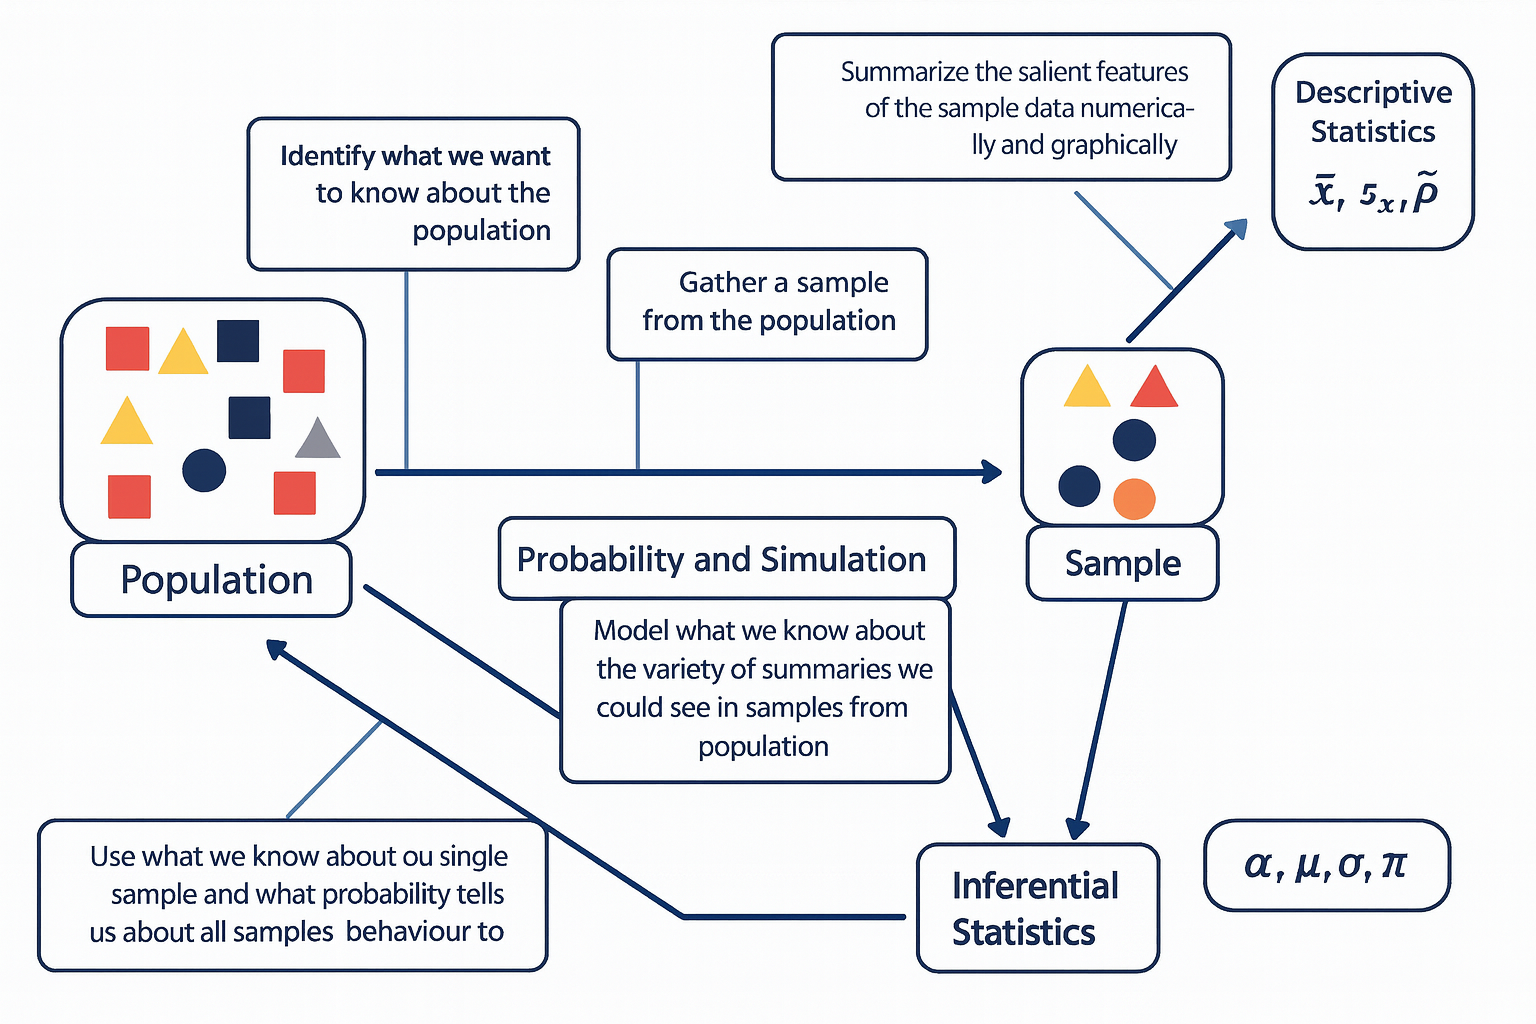
\includegraphics[keepaspectratio]{images/yek.png}}

\section{Gathering Data}\label{gathering-data}

The stepping stone towards conducting statistical analysis is collecting
data. The elegance of good research begins not with equations or
estimation models, but with the deliberate act of collecting or finding
the \emph{right} information. Whether searching for the relevant survey,
locating a reliable public dataset, or designing your own instrument to
capture social realities, data collection is the foundation upon which
all inference rests. This process is both scientific and creative---it
requires knowing what questions matter, where credible evidence resides,
and how to translate abstract ideas into measurable variables. Without
the discipline of gathering data carefully, analysis becomes
speculation. But when we gather the right data---accurate,
representative, and conceptually aligned---the analytical process
becomes not only possible but powerful.

What major survey datasets are publically available? Here are a list of
a few major survey datasets that are regularly used in social sciences.

\subsection{General Social Survey (GSS) *
US-based}\label{general-social-survey-gss-us-based}

The General Social Survey (GSS) is among the most influential and
long-standing social science data sources in the United States.
Conducted by the National Opinion Research Center (NORC) at the
University of Chicago since 1972, the GSS captures the shifting
landscape of American attitudes, behaviors, and beliefs. It is a
repeated cross-sectional survey, meaning that different representative
samples of U.S. adults are interviewed every one or two years. The GSS
includes a rich array of topics---ranging from political ideology,
social trust, racial attitudes, and gender norms to work, family, and
religion---making it indispensable for studying social change. It also
integrates modules from the International Social Survey Programme
(ISSP), enabling cross-national comparisons on topics such as
inequality, religion, and national identity. For decades, the GSS has
served as a barometer of American society, offering scholars a
consistent empirical foundation for studying how values and cleavages
evolve across generations.

\subsection{American National Election Studies (ANES) *
US-based}\label{american-national-election-studies-anes-us-based}

The American National Election Studies (ANES) are a cornerstone of
political behavior research in the United States. Established in 1948
and jointly administered by Stanford University and the University of
Michigan, ANES surveys collect rich pre- and post-election data to
understand how citizens form opinions, participate in politics, and make
electoral choices. The ANES includes detailed measures of political
ideology, media exposure, partisanship, policy preferences, and social
identity, along with contextual information about candidates and
campaigns. Its time-series design---fielded every national election
cycle---allows researchers to trace the evolution of political attitudes
and polarization in the U.S. over more than seven decades. Because of
its rigorous sampling, extensive questionnaire design, and continuity of
measures, ANES remains the definitive dataset for studying democratic
engagement, voter behavior, and the sociopolitical undercurrents shaping
American democracy. Current Population Survey (CPS) The Current
Population Survey (CPS), jointly conducted by the U.S. Census Bureau and
the Bureau of Labor Statistics, is the primary source of labor force
statistics in the United States. Since its inception in the 1940s, the
CPS has provided monthly data on employment, unemployment, earnings, and
demographic characteristics for a representative sample of roughly
60,000 U.S. households. In addition to the core labor force questions,
the CPS includes periodic supplements that cover vital social
topics---such as education, fertility, civic participation, and voting
behavior (the CPS Voting and Registration Supplement). Because of its
frequency, large sample size, and policy relevance, the CPS is essential
not only to economists and policymakers but also to sociologists and
demographers studying inequality, class mobility, and household dynamics
in real time.

\subsection{Panel Study of Income Dynamics (PSID) *
US-based}\label{panel-study-of-income-dynamics-psid-us-based}

The Panel Study of Income Dynamics (PSID), begun in 1968 at the
University of Michigan's Institute for Social Research, is one of the
longest-running household panel studies in the world. Unlike
cross-sectional surveys, the PSID follows the same families and their
descendants over decades, enabling the study of intergenerational
mobility, family formation, and long-term income dynamics. Its design
captures both economic and social dimensions of life---income,
employment, wealth, health, and housing---allowing researchers to trace
how structural inequality unfolds across generations. The PSID's
intergenerational structure has made it particularly valuable for
studying persistent poverty, wealth accumulation, and social
stratification within the U.S., and its supplements on child development
and transition to adulthood add depth to understanding life-course
processes.

\subsection{European Social Survey (ESS) *
Cross-National}\label{european-social-survey-ess-cross-national}

The European Social Survey (ESS), initiated in 2001, provides a gold
standard for cross-national research on social attitudes across Europe.
Conducted biennially across more than 30 European countries, the ESS
maintains strict methodological consistency, including face-to-face
interviews, high response rate standards, and meticulous translation
protocols to ensure cross-national comparability. Its thematic modules
examine values, trust in institutions, political engagement, migration,
and welfare attitudes, along with rotating modules on emerging social
issues such as climate change or digitalization. The ESS is widely
regarded as the premier data source for analyzing how social, political,
and cultural divides vary across European societies and welfare regimes.
Its rigorous methodological design has set a benchmark for international
survey research, making it a cornerstone for comparative sociology and
political science.

\subsection{International Social Survey Programme (ISSP) *
Cross-National}\label{international-social-survey-programme-issp-cross-national}

The International Social Survey Programme (ISSP) is a collaborative,
cross-national effort that began in 1984, bringing together social
science organizations from around the world to administer a common
module of questions each year. Unlike the ESS, which operates solely in
Europe, the ISSP has a truly global reach, including countries across
six continents. Each annual module focuses on a single theme---such as
social inequality, religion, national identity, or environmental
attitudes---and repeats every decade to measure change over time. The
ISSP's harmonized data allow for systematic comparison of social
attitudes across diverse political and cultural contexts, offering
unparalleled insight into how values and norms are shaped by
institutions and historical legacies. For scholars of comparative
sociology and globalization, the ISSP represents an indispensable tool
for studying how societies differ and evolve.

\subsection{World Values Survey (WVS) *
Cross-National}\label{world-values-survey-wvs-cross-national}

The World Values Survey (WVS) is an ambitious, long-running project that
seeks to map the cultural values and beliefs of people around the globe.
Initiated in 1981 and now spanning over 100 countries, the WVS measures
attitudes toward democracy, religion, gender roles, economic life, and
social trust. Its conceptual foundation builds on the idea that cultural
change and economic development are interconnected---an idea most
famously articulated by Ronald Inglehart's theory of postmaterialist
value change. Conducted in waves approximately every five years, the WVS
provides a comparative framework to examine how modernization,
globalization, and generational turnover reshape moral and political
orientations worldwide. Together with the ESS and ISSP, it forms a triad
of international surveys that collectively enable a global sociology of
values and social change.

\subsection{A Key Distinction Between the Types of
Studies}\label{a-key-distinction-between-the-types-of-studies}

A central distinction in social research lies between studies that
intervene in the social world and those that observe it as it naturally
unfolds. Experimental studies are designed to establish \emph{causal}
relationships: researchers deliberately manipulate one or more
variables---such as exposure to a message, allocation of resources, or
participation in a program---and then observe the resulting changes in
outcomes. In contrast, observational studies refrain from such
manipulation; they document social behavior, attitudes, or outcomes as
they occur in real life. While experiments offer stronger leverage for
identifying causality through control and randomization, observational
designs provide insights into complex social processes that cannot be
ethically or practically manipulated. Recognizing this distinction is
fundamental, as it shapes how researchers interpret evidence, evaluate
validity, and generalize findings to broader populations.

\subsection{Experiment}\label{experiment}

In social science, an experiment is a systematic study in which the
researcher deliberately introduces an intervention or treatment in order
to observe its causal effect on an outcome. The key feature of
experimentation is control---researchers manipulate one or more
independent variables while holding other factors constant, allowing for
the identification of causal relationships.

Example: A sociologist wants to examine whether exposure to news stories
about economic inequality affects people's support for redistributive
policies. Participants are randomly assigned to read one of five news
articles---each emphasizing a different narrative about inequality---and
then asked about their policy preferences. Because the researcher
actively manipulates what participants are exposed to, this constitutes
an experiment. Observational Study

An observational study involves collecting data without manipulating or
altering the social processes under investigation. Researchers observe
patterns, behaviors, or associations as they naturally occur, rather
than imposing an intervention. This design is often used when
experimental manipulation would be unethical or impractical.

\emph{Example}: A political scientist wants to know whether residents of
wealthier neighborhoods are more likely to vote. They collect
information from voter registration records and census data, comparing
turnout rates across neighborhoods with different socioeconomic
profiles. Because the researcher merely observes existing differences
without assigning any treatment, this is an observational study.

\subsection{Sample}\label{sample-1}

A sample is a subset of a broader population that researchers study in
order to make inferences about that population. Because it is rarely
possible to collect information from every individual in a population,
sampling allows researchers to study social phenomena efficiently while
maintaining representativeness. Simple Random Sample (SRS)

A simple random sample (SRS) is a sampling method in which every
possible subset of the population of a given size has an equal chance of
being selected. This procedure minimizes selection bias and ensures that
observed patterns can be attributed to the population rather than to
systematic differences in who was included.

\emph{Example}: To study public attitudes toward climate change, a
researcher draws a random sample of 1,500 adults from a national
database where each individual has an equal probability of being chosen.
This kind of sampling forms the statistical foundation for most
nationally representative surveys in the social sciences, such as the
General Social Survey or European Social Survey.

\section{Summarizing Data}\label{summarizing-data}

In any empirical investigation, one of the first steps is to summarize
information about the units or individuals we study. Social scientists
often distinguish between characteristics of an entire population and
those of a sample drawn from it. The key concepts here are parameters
and statistics---two closely related but conceptually distinct ideas
that link description and inference.

A \textbf{\emph{parameter}} is a numerical summary that describes a true
characteristic of the entire population---the full set of individuals,
organizations, or events that constitute our field of interest. In
practice, parameters are almost always unknown because it is rarely
feasible to collect information on every member of a population. For
example, if we could measure the average income of all households in the
United States, that value would represent a population parameter.
Likewise, the mean level of political trust among all adults in a
country, or the proportion of citizens who voted in a specific election,
are parameters describing entire populations.

A \textbf{\emph{statistic}}, by contrast, is a numerical summary
computed from a sample---a smaller subset of observations selected from
the population. Because researchers typically rely on samples to study
larger populations, sample statistics serve as our best estimates of the
unknown population parameters. For instance, the average income
calculated from a nationally representative survey, such as the General
Social Survey, is a sample statistic that approximates the population
mean. Similarly, if we surveyed a thousand voters to estimate the
proportion who support a particular candidate, that proportion would be
a statistic, standing in for the true but unknown population value.

The relationship between populations and samples is often visualized as
a flow of information: on one side lies the broad and complex population
we seek to understand, and on the other, the smaller and more manageable
sample we can actually observe. Between the two stands the domain of
probability and simulation, which provides the theoretical bridge
linking what we see to what we infer. Probability theory helps us
quantify how much variation we might expect if we were to draw many
different samples from the same population. Through simulation and
modeling, researchers can approximate this sampling variability, giving
rise to measures of uncertainty such as confidence intervals and
standard errors.

Together, these elements---parameters and statistics, sampling and
inference---form the intellectual architecture of social statistics.
They remind us that every conclusion we draw about society rests on a
bridge between what we observe and what we infer, linking empirical data
to theoretical understanding through the language of probability.

\section{Types of Variables/Data}\label{types-of-variablesdata}

In social science research, variables can take many forms depending on
what they measure and how those measurements are expressed.
Distinguishing among types of data is crucial because it determines
which statistical summaries, visualizations, and models are appropriate
for analysis. Broadly speaking, data can be classified into two
overarching types: quantitative (numerical) and qualitative
(categorical).

\subsection{Quantitative (Numerical)
Data}\label{quantitative-numerical-data}

Quantitative data consist of numerical values that express how much or
how many of something there is. These values exist on a numeric scale
with meaningful magnitudes, allowing for arithmetic operations such as
addition or averaging. Quantitative data can be further divided into two
subtypes: Discrete data represent countable quantities that take on
distinct, separate values---often integers---with gaps between them.
Examples include the number of children in a household, the count of
protests in a county, or the number of campaign events attended by a
candidate. Because these variables reflect counts, fractional values
have no substantive meaning.

Continuous data represent measurements that can, in principle, take on
any value within a given interval. There are no inherent gaps in the
scale; instead, the precision of measurement depends on the accuracy of
the instrument or method used. Examples include age (measured in years,
months, or days), household income, or hours of television watched per
week. Continuous variables are especially common in survey and
administrative data when researchers measure social or economic
quantities along a continuum.

\subsection{Qualitative (Categorical)
Data}\label{qualitative-categorical-data}

Qualitative or categorical data, by contrast, represent values that
differ in kind rather than degree. These data describe membership in
categories, groups, or qualitative states that cannot be meaningfully
ordered or subjected to arithmetic operations. Each distinct category is
referred to as a level of the variable. Examples include gender
identity, religious affiliation, race or ethnicity, political party, or
preferred news source.

\subsection{Within categorical data, researchers often distinguish
between:}\label{within-categorical-data-researchers-often-distinguish-between}

Nominal variables, where categories have no intrinsic order (e.g.,
political party: Democrat, Republican, Independent, Other), and Ordinal
variables, where categories imply a rank or order but the intervals
between them are not uniform (e.g., ideology scale: ``very liberal,''
``liberal,'' ``moderate,'' ``conservative,'' ``very conservative'').

\subsection{An Illustrative Example}\label{an-illustrative-example}

Consider a political scientist preparing to study voting behavior ahead
of a national election. They design a survey collecting a range of
variables about registered voters:

\begin{itemize}
\tightlist
\item
  \textbf{Party identification (Democrat, Republican, Independent,
  Other) --- categorical, nominal }
\item
  \textbf{Political ideology (very liberal to very conservative) ---
  categorical, ordinal }
\item
  \textbf{Voter turnout history (number of elections voted in during the
  past decade) --- quantitative, discrete }
\item
  \textbf{Campaign donations (dollar amount contributed to political
  campaigns) --- quantitative, continuous }
\item
  \textbf{Primary news source (television, online, print, social media)
  --- categorical, nominal }
\item
  \textbf{Age (in years) --- quantitative, continuous }
\item
  \textbf{Education (less than high school, high school, some college,
  college degree, graduate degree) --- categorical, ordinal }
\end{itemize}

This list is meant to provide the level of measurement for each
variable---nominal, ordinal, binary, discrete, or continuous.

Understanding these distinctions is more than a technical exercise: it
informs every step of analysis, from selecting the right summary
statistics and visualizations (e.g., bar charts versus histograms) to
choosing the appropriate inferential tests (e.g., chi-square,
correlation, or regression). In short, recognizing the type of data at
hand is a foundational skill for designing, interpreting, and
communicating sound social research.

\section{In-Class Exercise (1): Identifying Variable
Types}\label{in-class-exercise-1-identifying-variable-types}

In this exercise, you will practice classifying variables by their level
of measurement---a foundational skill for all empirical social
scientists. The table below lists variables drawn from a hypothetical
study of registered voters in an upcoming general election. Each
variable reflects a different kind of information political researchers
might collect: from demographic traits and political attitudes to
behaviors such as voting and campaign participation.

Your task is to identify the correct variable type for each entry in the
table---whether it is nominal, ordinal, binary, discrete, or continuous.
Think carefully about what distinguishes each level of measurement. Ask
yourself:

\begin{itemize}
\tightlist
\item
  \textbf{Does the variable represent categories or quantities? }
\item
  \textbf{If it's categorical, does it have a natural order (ordinal) or
  not (nominal)? }
\item
  \textbf{If it's numeric, does it take on only whole numbers (discrete)
  or any value along a scale (continuous)? }
\item
  \textbf{Discuss your reasoning with your classmates and be prepared to
  explain how your classification would influence the choice of graphs
  or statistical models in a real research project. }
\end{itemize}

\begin{longtable}[]{@{}lc@{}}
\caption{Population: Registered voters in the upcoming general election
--- Identify each as nominal, ordinal, binary, discrete, or
continuous.}\tabularnewline
\toprule\noalign{}
Variables / Characteristics & Variable Type \\
\midrule\noalign{}
\endfirsthead
\toprule\noalign{}
Variables / Characteristics & Variable Type \\
\midrule\noalign{}
\endhead
\bottomrule\noalign{}
\endlastfoot
Party identification (Dem/Rep/Ind/Other) & \_\_\_\_\_\_\_\_\_\_ \\
Ideology (1 = liberal \ldots{} 7 = conservative) &
\_\_\_\_\_\_\_\_\_\_ \\
Voted in last midterm (Yes/No) & \_\_\_\_\_\_\_\_\_\_ \\
Age (in years) & \_\_\_\_\_\_\_\_\_\_ \\
Household income bracket & \_\_\_\_\_\_\_\_\_\_ \\
Number of political meetings attended last year &
\_\_\_\_\_\_\_\_\_\_ \\
Primary news source (TV/Online/Print/Radio) & \_\_\_\_\_\_\_\_\_\_ \\
Zip code / precinct & \_\_\_\_\_\_\_\_\_\_ \\
Support for Policy X (0--100 thermometer) & \_\_\_\_\_\_\_\_\_\_ \\
Campaign donations last 12 months (USD) & \_\_\_\_\_\_\_\_\_\_ \\
\end{longtable}

\section{In-Class Exercise (2):: The 1936 FDR--Landon
Poll}\label{in-class-exercise-2-the-1936-fdrlandon-poll}

During the 1936 U.S. presidential election between Democratic incumbent
Franklin D. Roosevelt (FDR) and Republican challenger Alf Landon, The
Literary Digest magazine conducted a massive poll to predict the
outcome. The magazine mailed 10 million questionnaires to names drawn
from its subscriber list, telephone directories, and automobile
registration records. About 2.3 million people responded. Based on these
replies, the Digest predicted that Landon would win by a landslide of
370 electoral votes. In contrast, George Gallup, using a carefully
designed random sample of about 50,000 respondents, correctly predicted
that Roosevelt would win decisively. Learning Goal: This example
illustrates how even a very large dataset can lead to inaccurate
conclusions if the sample is not representative of the population of
interest. It highlights the importance of sampling design and bias in
survey research.

Questions:

\begin{itemize}
\tightlist
\item
  \textbf{Identify the population(s) and parameter(s) of interest to The
  Literary Digest. }
\item
  \textbf{Was the data collection observational or experimental? Explain
  your reasoning? }
\item
  \textbf{Describe the sample and the type of data obtained }
\item
  \textbf{What does this example teach us about the relationship between
  sample size and sample quality in public opinion research? }
\end{itemize}

Extension Activity: Have students compare The Literary Digest poll to a
modern equivalent, such as online opt-in surveys. Discuss how selection
bias can still occur today even with large datasets.

\section{A First Look at R and
RStudio}\label{a-first-look-at-r-and-rstudio}

\subsection{Part 1 --- Set up your
workspace}\label{part-1-set-up-your-workspace}

\section{A First Look at R and
RStudio}\label{a-first-look-at-r-and-rstudio-1}

This chapter guides you through setting up the necessary software for
this book. We strongly recommend using \textbf{RStudio Projects} to
manage your files, which ensures all examples are reproducible.

\subsection{Part 1 --- Set Up Your Workspace
🛠️}\label{part-1-set-up-your-workspace-1}

\subsubsection{1. Prepare Your Course
Folder}\label{prepare-your-course-folder}

Start by creating a main location for all your files.

\begin{enumerate}
\def\labelenumi{\arabic{enumi}.}
\tightlist
\item
  \textbf{Create a main class folder} on your computer (e.g., on your
  Desktop or in Documents). Name it something easy to find, like
  \textbf{\texttt{Stats\_Book}} or \textbf{\texttt{SOC205A\_Data}}.
\item
  All files, projects, and data for this course will be saved
  \emph{inside} this folder.
\end{enumerate}

\begin{center}\rule{0.5\linewidth}{0.5pt}\end{center}

\subsubsection{2. Install the Core
Software}\label{install-the-core-software}

You need both \textbf{R} (the statistical programming language) and
\textbf{RStudio} (the user interface, or IDE).

\begin{tcolorbox}[enhanced jigsaw, left=2mm, leftrule=.75mm, title=\textcolor{quarto-callout-important-color}{\faExclamation}\hspace{0.5em}{Important}, titlerule=0mm, toprule=.15mm, colframe=quarto-callout-important-color-frame, opacitybacktitle=0.6, bottomtitle=1mm, rightrule=.15mm, colbacktitle=quarto-callout-important-color!10!white, toptitle=1mm, arc=.35mm, colback=white, opacityback=0, bottomrule=.15mm, breakable, coltitle=black]

\textbf{Installation Order Matters!} You must install \textbf{R first},
and then \textbf{RStudio Desktop}.

\begin{enumerate}
\def\labelenumi{\arabic{enumi}.}
\tightlist
\item
  \textbf{Install R} (The Language): Search ``Install R'' and follow the
  link to CRAN (The Comprehensive R Archive Network).
\item
  \textbf{Install RStudio Desktop} (The IDE): Search ``Install RStudio
  Desktop'' and select the \textbf{Free/Open Source} edition.
\end{enumerate}

\end{tcolorbox}

\begin{center}\rule{0.5\linewidth}{0.5pt}\end{center}

\subsubsection{3. Start RStudio and Create a
Project}\label{start-rstudio-and-create-a-project}

RStudio Projects keep your files and paths organized, which is essential
when compiling a book.

\begin{enumerate}
\def\labelenumi{\arabic{enumi}.}
\tightlist
\item
  \textbf{Launch RStudio.}
\item
  Go to the menu: \textbf{File} \(\to\) \textbf{New Project} \(\to\)
  \textbf{New Directory} \(\to\) \textbf{New Project}.
\item
  \textbf{Name the project} (e.g., \texttt{lecture-1}).
\item
  For the location, choose the \textbf{main class folder} you created in
  Step 1.
\item
  Click \textbf{Create Project}.
\end{enumerate}

\begin{center}\rule{0.5\linewidth}{0.5pt}\end{center}

\subsubsection{4. Sanity Check: Verify R is
Working}\label{sanity-check-verify-r-is-working}

Use the R Console to confirm that R is installed correctly and is
accessible by RStudio.

\begin{enumerate}
\def\labelenumi{\arabic{enumi}.}
\tightlist
\item
  Look at the \textbf{R Console} (usually the bottom-left pane).
\item
  Type the following command \textbf{exactly} and press \textbf{Enter}:
\end{enumerate}

To begin, create a new R Markdown file in RStudio. From the menu, select
File ▸ New File ▸ R Markdown\ldots, and when prompted, give your
document a title such as Lecture 1 Practice. You may choose any output
format---Word or PDF is recommended for simplicity, though HTML also
works. Once the file opens, save it immediately into your designated
class folder with a clear name like Lecture1.Rmd. Next, scroll through
the automatically generated template and delete everything beginning
with the line \#\# R Markdown to the end of the file, leaving only the
YAML header at the top. This ensures you're starting with a clean
workspace. Finally, click Knit to compile the document. If your setup is
correct, a Word, PDF, or HTML file with the same name should appear in
your folder. Open it to confirm that RStudio successfully created your
first document.

With your document ready, you will now explore one of R's classic
built-in datasets, called iris. This dataset contains measurements of
150 individual irises, divided into three species. To view the data,
create a code chunk---either by selecting Code ▸ Insert Chunk from the
menu or by typing the shortcut (Ctrl+Alt+I or ⌘⌥I). Inside this code
chunk, type print(iris) and run the chunk to display the full dataset in
the console. Observe that there are 150 rows representing flowers and 5
variables: (1) Sepal Length, (2) Sepal Width, (3) Petal Length, (4)
Petal Width, and (5) Species. The first four variables are quantitative
and continuous, while Species is a categorical variable with three
distinct levels (setosa, versicolor, and virginica).

Next, examine the structure of the dataset by typing str(iris) in the
same or a new code chunk. Running this command reveals the data types of
each variable and confirms your earlier observations about their
nature---numeric for the first four and factor (categorical) for the
fifth. To go a step further, type summary(iris) and execute the command.
This function provides numerical summaries for each quantitative
variable---displaying the minimum, first quartile, median, mean, third
quartile, and maximum---and shows counts for each level of the
categorical variable. Discuss with students how summary() automatically
adjusts its output depending on variable type, giving a concise overview
of both numeric distributions and categorical frequencies.

Once you have run and interpreted these commands, include short written
explanations in your R Markdown document to describe what each function
does and what you observe in the results. When finished, knit the file
again and check the output. You now have your first reproducible R
document, complete with code, output, and interpretation. oduce and/or
explain your code outside of the code chunk. Knit the word document.

\section{Working With Real World Dataset: The Iris
Data}\label{working-with-real-world-dataset-the-iris-data}

The Iris dataset is one of the most well-known datasets in statistics
and data science. It contains measurements of iris flowers collected to
study how physical characteristics vary across different species.
Originally compiled by the British statistician and biologist Ronald A.
Fisher in 1936, the dataset was introduced in his classic paper ``The
Use of Multiple Measurements in Taxonomic Problems.'' Fisher used these
data to demonstrate one of the earliest applications of discriminant
analysis, a statistical method for classifying observations into
categories based on quantitative traits. The dataset includes 150
individual iris flowers, divided equally among three species:

*\textbf{Iris setosa}

*\textbf{Iris versicolor}

*\textbf{Iris virginica}

For each flower, Fisher measured four quantitative variables:

*\textbf{Sepal Length (in centimeters)}

*\textbf{Sepal Width (in centimeters)}

*\textbf{Petal Length (in centimeters)}

*\textbf{Petal Width (in centimeters)}

These measurements describe the geometry of the flowers' petals and
sepals---two key parts of the blossom that vary visibly across species.
Using these traits, Fisher showed how statistical models could classify
species based on measurement patterns, a concept that later became
foundational in machine learning and pattern recognition.

Today, the Iris dataset comes preloaded with R and most statistical
software. It continues to serve as a pedagogical example for teaching
data exploration, visualization, descriptive statistics, classification,
and clustering. Although small in size, it captures many of the
essential elements of real-world data: multiple variables, distinct
categories, and measurable variation within and between groups.

The dataset was originally introduced by the British biologist and
statistician Ronald A. Fisher in his 1936 paper, ``The Use of Multiple
Measurements in Taxonomic Problems.'' Fisher used these data to
demonstrate one of the first applications of discriminant analysis, a
method for classifying observations into groups.

The dataset contains 150 observations of iris flowers, equally divided
among three species: Iris setosa, Iris versicolor, and Iris virginica.
For each flower, Fisher recorded four quantitative measurements---sepal
length, sepal width, petal length, and petal width---all in centimeters.
These measurements were collected from real specimens and became a
foundational example for studying classification, clustering, and
statistical inference.

In R, the data are stored as a data frame (a rectangular table similar
to a spreadsheet). Because it's built into R, you can explore it right
away:

\section{Eseential Commands in R}\label{eseential-commands-in-r}

\subsection{Accessing help}\label{accessing-help}

Use ? or help() to pull up documentation; ?? searches help topics.

\begin{Shaded}
\begin{Highlighting}[]
\NormalTok{?iris                  }\CommentTok{\# help page for the dataset}
\NormalTok{?data.frame            }\CommentTok{\# help page for data frames}
\FunctionTok{help}\NormalTok{(}\StringTok{"subset"}\NormalTok{)         }\CommentTok{\# equivalent}
\NormalTok{??}\StringTok{"linear model"}       \CommentTok{\# fuzzy search across help files}
\end{Highlighting}
\end{Shaded}

\subsection{Learning the dataset - Summary
Statistics}\label{learning-the-dataset---summary-statistics}

\begin{Shaded}
\begin{Highlighting}[]
\CommentTok{\# loads the dataset (though usually it’s already available)}
\FunctionTok{data}\NormalTok{(iris)    }
\CommentTok{\# shows the first six rows {-} get a sens eof the dataset }
\FunctionTok{head}\NormalTok{(iris)     }
\end{Highlighting}
\end{Shaded}

\begin{verbatim}
  Sepal.Length Sepal.Width Petal.Length Petal.Width Species
1          5.1         3.5          1.4         0.2  setosa
2          4.9         3.0          1.4         0.2  setosa
3          4.7         3.2          1.3         0.2  setosa
4          4.6         3.1          1.5         0.2  setosa
5          5.0         3.6          1.4         0.2  setosa
6          5.4         3.9          1.7         0.4  setosa
\end{verbatim}

\subsection{Information about objects}\label{information-about-objects}

str(), class(), names(), dim(), and summary() give fast overviews.

\begin{Shaded}
\begin{Highlighting}[]
\CommentTok{\# structure (types + preview) {-} it gives you an overview of the dataset }
\FunctionTok{str}\NormalTok{(iris)  }
\end{Highlighting}
\end{Shaded}

\begin{verbatim}
'data.frame':   150 obs. of  5 variables:
 $ Sepal.Length: num  5.1 4.9 4.7 4.6 5 5.4 4.6 5 4.4 4.9 ...
 $ Sepal.Width : num  3.5 3 3.2 3.1 3.6 3.9 3.4 3.4 2.9 3.1 ...
 $ Petal.Length: num  1.4 1.4 1.3 1.5 1.4 1.7 1.4 1.5 1.4 1.5 ...
 $ Petal.Width : num  0.2 0.2 0.2 0.2 0.2 0.4 0.3 0.2 0.2 0.1 ...
 $ Species     : Factor w/ 3 levels "setosa","versicolor",..: 1 1 1 1 1 1 1 1 1 1 ...
\end{verbatim}

\begin{Shaded}
\begin{Highlighting}[]
\CommentTok{\# it tells you the types of dataset you are working with }
\FunctionTok{class}\NormalTok{(iris)   }
\end{Highlighting}
\end{Shaded}

\begin{verbatim}
[1] "data.frame"
\end{verbatim}

\begin{Shaded}
\begin{Highlighting}[]
\CommentTok{\# it tells you the name fo the columns in the dataset }
\FunctionTok{names}\NormalTok{(iris)  }
\end{Highlighting}
\end{Shaded}

\begin{verbatim}
[1] "Sepal.Length" "Sepal.Width"  "Petal.Length" "Petal.Width"  "Species"     
\end{verbatim}

\begin{Shaded}
\begin{Highlighting}[]
\CommentTok{\# it tells you the number of rows and columns your dataset.  }
\FunctionTok{dim}\NormalTok{(iris)   }
\end{Highlighting}
\end{Shaded}

\begin{verbatim}
[1] 150   5
\end{verbatim}

\begin{Shaded}
\begin{Highlighting}[]
\CommentTok{\# it tells you the numeric summaries + factor counts}
\FunctionTok{summary}\NormalTok{(iris)          }
\end{Highlighting}
\end{Shaded}

\begin{verbatim}
  Sepal.Length    Sepal.Width     Petal.Length    Petal.Width   
 Min.   :4.300   Min.   :2.000   Min.   :1.000   Min.   :0.100  
 1st Qu.:5.100   1st Qu.:2.800   1st Qu.:1.600   1st Qu.:0.300  
 Median :5.800   Median :3.000   Median :4.350   Median :1.300  
 Mean   :5.843   Mean   :3.057   Mean   :3.758   Mean   :1.199  
 3rd Qu.:6.400   3rd Qu.:3.300   3rd Qu.:5.100   3rd Qu.:1.800  
 Max.   :7.900   Max.   :4.400   Max.   :6.900   Max.   :2.500  
       Species  
 setosa    :50  
 versicolor:50  
 virginica :50  
                
                
                
\end{verbatim}

\subsection{Using packages}\label{using-packages}

Install once; load each session. (Skip install.packages() on shared lab
machines if preinstalled.)

\begin{Shaded}
\begin{Highlighting}[]
\CommentTok{\# The first command installs the package. The second command (library) "calls" it. }

\FunctionTok{install.packages}\NormalTok{(}\StringTok{"tidyverse"}\NormalTok{)   }\CommentTok{\# uncomment if needed}
\end{Highlighting}
\end{Shaded}

\begin{verbatim}
The following package(s) will be installed:
- tidyverse [2.0.0]
These packages will be installed into "~/Documents/UCSB/book/r-book-starter/renv/library/macos/R-4.5/aarch64-apple-darwin20".

# Installing packages --------------------------------------------------------
- Installing tidyverse ...                      OK [linked from cache]
Successfully installed 1 package in 2.6 milliseconds.
\end{verbatim}

\begin{Shaded}
\begin{Highlighting}[]
\FunctionTok{library}\NormalTok{(tidyverse)                }\CommentTok{\# loads dplyr, ggplot2, etc.}
\end{Highlighting}
\end{Shaded}

\subsection{The working directory}\label{the-working-directory}

\begin{Shaded}
\begin{Highlighting}[]
\CommentTok{\# tells you your current working directory}
\FunctionTok{getwd}\NormalTok{()     }\CommentTok{\# setwd("\textasciitilde{}/Stats\_Class")  \# avoid hard{-}coding; use Projects instead}
\end{Highlighting}
\end{Shaded}

\begin{verbatim}
[1] "/Users/masoudmovahed/Documents/UCSB/book/r-book-starter"
\end{verbatim}

\subsection{Operators (arithmetic, relational, logical,
assignment)}\label{operators-arithmetic-relational-logical-assignment}

\begin{Shaded}
\begin{Highlighting}[]
\CommentTok{\# Create two numeric vectors from iris so we can practice operations.}
\NormalTok{x }\OtherTok{\textless{}{-}}\NormalTok{ iris}\SpecialCharTok{$}\NormalTok{Sepal.Length}
\NormalTok{y }\OtherTok{\textless{}{-}}\NormalTok{ iris}\SpecialCharTok{$}\NormalTok{Petal.Length}

\CommentTok{\# Add two numeric vectors element{-}by{-}element (quick math across rows).}
\NormalTok{x }\SpecialCharTok{+}\NormalTok{ y}
\end{Highlighting}
\end{Shaded}

\begin{verbatim}
  [1]  6.5  6.3  6.0  6.1  6.4  7.1  6.0  6.5  5.8  6.4  6.9  6.4  6.2  5.4  7.0
 [16]  7.2  6.7  6.5  7.4  6.6  7.1  6.6  5.6  6.8  6.7  6.6  6.6  6.7  6.6  6.3
 [31]  6.4  6.9  6.7  6.9  6.4  6.2  6.8  6.3  5.7  6.6  6.3  5.8  5.7  6.6  7.0
 [46]  6.2  6.7  6.0  6.8  6.4 11.7 10.9 11.8  9.5 11.1 10.2 11.0  8.2 11.2  9.1
 [61]  8.5 10.1 10.0 10.8  9.2 11.1 10.1  9.9 10.7  9.5 10.7 10.1 11.2 10.8 10.7
 [76] 11.0 11.6 11.7 10.5  9.2  9.3  9.2  9.7 11.1  9.9 10.5 11.4 10.7  9.7  9.5
 [91]  9.9 10.7  9.8  8.3  9.8  9.9  9.9 10.5  8.1  9.8 12.3 10.9 13.0 11.9 12.3
[106] 14.2  9.4 13.6 12.5 13.3 11.6 11.7 12.3 10.7 10.9 11.7 12.0 14.4 14.6 11.0
[121] 12.6 10.5 14.4 11.2 12.4 13.2 11.0 11.0 12.0 13.0 13.5 14.3 12.0 11.4 11.7
[136] 13.8 11.9 11.9 10.8 12.3 12.3 12.0 10.9 12.7 12.4 11.9 11.3 11.7 11.6 11.0
\end{verbatim}

\begin{Shaded}
\begin{Highlighting}[]
\CommentTok{\# Ask a yes/no question per row: is Sepal.Length \textgreater{} 6? Returns TRUE/FALSE.}
\NormalTok{x }\SpecialCharTok{\textgreater{}} \DecValTok{6}
\end{Highlighting}
\end{Shaded}

\begin{verbatim}
  [1] FALSE FALSE FALSE FALSE FALSE FALSE FALSE FALSE FALSE FALSE FALSE FALSE
 [13] FALSE FALSE FALSE FALSE FALSE FALSE FALSE FALSE FALSE FALSE FALSE FALSE
 [25] FALSE FALSE FALSE FALSE FALSE FALSE FALSE FALSE FALSE FALSE FALSE FALSE
 [37] FALSE FALSE FALSE FALSE FALSE FALSE FALSE FALSE FALSE FALSE FALSE FALSE
 [49] FALSE FALSE  TRUE  TRUE  TRUE FALSE  TRUE FALSE  TRUE FALSE  TRUE FALSE
 [61] FALSE FALSE FALSE  TRUE FALSE  TRUE FALSE FALSE  TRUE FALSE FALSE  TRUE
 [73]  TRUE  TRUE  TRUE  TRUE  TRUE  TRUE FALSE FALSE FALSE FALSE FALSE FALSE
 [85] FALSE FALSE  TRUE  TRUE FALSE FALSE FALSE  TRUE FALSE FALSE FALSE FALSE
 [97] FALSE  TRUE FALSE FALSE  TRUE FALSE  TRUE  TRUE  TRUE  TRUE FALSE  TRUE
[109]  TRUE  TRUE  TRUE  TRUE  TRUE FALSE FALSE  TRUE  TRUE  TRUE  TRUE FALSE
[121]  TRUE FALSE  TRUE  TRUE  TRUE  TRUE  TRUE  TRUE  TRUE  TRUE  TRUE  TRUE
[133]  TRUE  TRUE  TRUE  TRUE  TRUE  TRUE FALSE  TRUE  TRUE  TRUE FALSE  TRUE
[145]  TRUE  TRUE  TRUE  TRUE  TRUE FALSE
\end{verbatim}

\begin{Shaded}
\begin{Highlighting}[]
\CommentTok{\# Combine two conditions: long sepals AND species is setosa (both must be true).}
\NormalTok{x }\SpecialCharTok{\textgreater{}} \DecValTok{6} \SpecialCharTok{\&}\NormalTok{ iris}\SpecialCharTok{$}\NormalTok{Species }\SpecialCharTok{==} \StringTok{"setosa"}
\end{Highlighting}
\end{Shaded}

\begin{verbatim}
  [1] FALSE FALSE FALSE FALSE FALSE FALSE FALSE FALSE FALSE FALSE FALSE FALSE
 [13] FALSE FALSE FALSE FALSE FALSE FALSE FALSE FALSE FALSE FALSE FALSE FALSE
 [25] FALSE FALSE FALSE FALSE FALSE FALSE FALSE FALSE FALSE FALSE FALSE FALSE
 [37] FALSE FALSE FALSE FALSE FALSE FALSE FALSE FALSE FALSE FALSE FALSE FALSE
 [49] FALSE FALSE FALSE FALSE FALSE FALSE FALSE FALSE FALSE FALSE FALSE FALSE
 [61] FALSE FALSE FALSE FALSE FALSE FALSE FALSE FALSE FALSE FALSE FALSE FALSE
 [73] FALSE FALSE FALSE FALSE FALSE FALSE FALSE FALSE FALSE FALSE FALSE FALSE
 [85] FALSE FALSE FALSE FALSE FALSE FALSE FALSE FALSE FALSE FALSE FALSE FALSE
 [97] FALSE FALSE FALSE FALSE FALSE FALSE FALSE FALSE FALSE FALSE FALSE FALSE
[109] FALSE FALSE FALSE FALSE FALSE FALSE FALSE FALSE FALSE FALSE FALSE FALSE
[121] FALSE FALSE FALSE FALSE FALSE FALSE FALSE FALSE FALSE FALSE FALSE FALSE
[133] FALSE FALSE FALSE FALSE FALSE FALSE FALSE FALSE FALSE FALSE FALSE FALSE
[145] FALSE FALSE FALSE FALSE FALSE FALSE
\end{verbatim}

\begin{Shaded}
\begin{Highlighting}[]
\CommentTok{\# Store the average of Sepal.Length so we can reuse it (one number).}
\NormalTok{x\_mean }\OtherTok{\textless{}{-}} \FunctionTok{mean}\NormalTok{(x)}

\CommentTok{\# Center each value: “how far is each observation from the average?”}
\NormalTok{x\_centered }\OtherTok{\textless{}{-}}\NormalTok{ x }\SpecialCharTok{{-}}\NormalTok{ x\_mean}

\CommentTok{\# Show the first few centered values so I can sanity{-}check the result quickly.}
\FunctionTok{head}\NormalTok{(x\_centered)}
\end{Highlighting}
\end{Shaded}

\begin{verbatim}
[1] -0.7433333 -0.9433333 -1.1433333 -1.2433333 -0.8433333 -0.4433333
\end{verbatim}

\subsection{Getting started with
vectors}\label{getting-started-with-vectors}

\begin{Shaded}
\begin{Highlighting}[]
\CommentTok{\# Make a tiny numeric vector by hand to see how vectors behave.}
\NormalTok{v }\OtherTok{\textless{}{-}} \FunctionTok{c}\NormalTok{(}\DecValTok{1}\NormalTok{, }\FloatTok{3.5}\NormalTok{, }\DecValTok{7}\NormalTok{)}

\CommentTok{\# Tell me how many elements are in this vector.}
\FunctionTok{length}\NormalTok{(v)}
\end{Highlighting}
\end{Shaded}

\begin{verbatim}
[1] 3
\end{verbatim}

\begin{Shaded}
\begin{Highlighting}[]
\CommentTok{\# Tell me the storage type (numeric, character, logical, etc.).}
\FunctionTok{class}\NormalTok{(v)}
\end{Highlighting}
\end{Shaded}

\begin{verbatim}
[1] "numeric"
\end{verbatim}

\begin{Shaded}
\begin{Highlighting}[]
\CommentTok{\# Coerce to integer so I see how R converts numeric types.}
\FunctionTok{as.integer}\NormalTok{(v)}
\end{Highlighting}
\end{Shaded}

\begin{verbatim}
[1] 1 3 7
\end{verbatim}

\begin{Shaded}
\begin{Highlighting}[]
\CommentTok{\# Show unique category labels present in Species (factor levels as characters).}
\FunctionTok{unique}\NormalTok{(iris}\SpecialCharTok{$}\NormalTok{Species)}
\end{Highlighting}
\end{Shaded}

\begin{verbatim}
[1] setosa     versicolor virginica 
Levels: setosa versicolor virginica
\end{verbatim}

\section{Selecting vector elements}\label{selecting-vector-elements}

\begin{Shaded}
\begin{Highlighting}[]
\CommentTok{\# Work with a single numeric column so indexing feels concrete.}
\NormalTok{x }\OtherTok{\textless{}{-}}\NormalTok{ iris}\SpecialCharTok{$}\NormalTok{Sepal.Width}

\CommentTok{\# Give me the very first value (position 1).}
\NormalTok{x[}\DecValTok{1}\NormalTok{]}
\end{Highlighting}
\end{Shaded}

\begin{verbatim}
[1] 3.5
\end{verbatim}

\begin{Shaded}
\begin{Highlighting}[]
\CommentTok{\# Give me the first five values (a range slice).}
\NormalTok{x[}\DecValTok{1}\SpecialCharTok{:}\DecValTok{5}\NormalTok{]}
\end{Highlighting}
\end{Shaded}

\begin{verbatim}
[1] 3.5 3.0 3.2 3.1 3.6
\end{verbatim}

\begin{Shaded}
\begin{Highlighting}[]
\CommentTok{\# Give me all widths strictly greater than 3.5 (logical filter).}
\NormalTok{x[x }\SpecialCharTok{\textgreater{}} \FloatTok{3.5}\NormalTok{]}
\end{Highlighting}
\end{Shaded}

\begin{verbatim}
 [1] 3.6 3.9 3.7 4.0 4.4 3.9 3.8 3.8 3.7 3.6 4.1 4.2 3.6 3.8 3.8 3.7 3.6 3.8 3.8
\end{verbatim}

\begin{Shaded}
\begin{Highlighting}[]
\CommentTok{\# Give me the single value that is the maximum (position of the max, then extract).}
\NormalTok{x[}\FunctionTok{which.max}\NormalTok{(x)]}
\end{Highlighting}
\end{Shaded}

\begin{verbatim}
[1] 4.4
\end{verbatim}

\begin{Shaded}
\begin{Highlighting}[]
\CommentTok{\# Chain two filters: take Sepal.Length from only virginica, then peek at first five.}
\NormalTok{iris}\SpecialCharTok{$}\NormalTok{Sepal.Length[iris}\SpecialCharTok{$}\NormalTok{Species }\SpecialCharTok{==} \StringTok{"virginica"}\NormalTok{][}\DecValTok{1}\SpecialCharTok{:}\DecValTok{5}\NormalTok{]}
\end{Highlighting}
\end{Shaded}

\begin{verbatim}
[1] 6.3 5.8 7.1 6.3 6.5
\end{verbatim}

\section{Math functions (on numeric
columns)}\label{math-functions-on-numeric-columns}

\begin{Shaded}
\begin{Highlighting}[]
\CommentTok{\# Central tendency: the typical Petal.Width.}
\FunctionTok{mean}\NormalTok{(iris}\SpecialCharTok{$}\NormalTok{Petal.Width)}
\end{Highlighting}
\end{Shaded}

\begin{verbatim}
[1] 1.199333
\end{verbatim}

\begin{Shaded}
\begin{Highlighting}[]
\CommentTok{\# Robust central tendency (less sensitive to outliers).}
\FunctionTok{median}\NormalTok{(iris}\SpecialCharTok{$}\NormalTok{Petal.Width)}
\end{Highlighting}
\end{Shaded}

\begin{verbatim}
[1] 1.3
\end{verbatim}

\begin{Shaded}
\begin{Highlighting}[]
\CommentTok{\# Distribution landmarks: 25th, 50th, and 75th percentiles.}
\FunctionTok{quantile}\NormalTok{(iris}\SpecialCharTok{$}\NormalTok{Petal.Width, }\AttributeTok{probs =} \FunctionTok{c}\NormalTok{(.}\DecValTok{25}\NormalTok{, .}\DecValTok{5}\NormalTok{, .}\DecValTok{75}\NormalTok{))}
\end{Highlighting}
\end{Shaded}

\begin{verbatim}
25% 50% 75% 
0.3 1.3 1.8 
\end{verbatim}

\begin{Shaded}
\begin{Highlighting}[]
\CommentTok{\# Spread measures: how variable is Petal.Width?}
\FunctionTok{var}\NormalTok{(iris}\SpecialCharTok{$}\NormalTok{Petal.Width)}
\end{Highlighting}
\end{Shaded}

\begin{verbatim}
[1] 0.5810063
\end{verbatim}

\begin{Shaded}
\begin{Highlighting}[]
\FunctionTok{sd}\NormalTok{(iris}\SpecialCharTok{$}\NormalTok{Petal.Width)}
\end{Highlighting}
\end{Shaded}

\begin{verbatim}
[1] 0.7622377
\end{verbatim}

\begin{Shaded}
\begin{Highlighting}[]
\CommentTok{\# Extremes in one shot (min and max).}
\FunctionTok{range}\NormalTok{(iris}\SpecialCharTok{$}\NormalTok{Petal.Width)}
\end{Highlighting}
\end{Shaded}

\begin{verbatim}
[1] 0.1 2.5
\end{verbatim}

\begin{Shaded}
\begin{Highlighting}[]
\CommentTok{\# Linear association strength between two continuous variables.}
\FunctionTok{cor}\NormalTok{(iris}\SpecialCharTok{$}\NormalTok{Sepal.Length, iris}\SpecialCharTok{$}\NormalTok{Petal.Length)}
\end{Highlighting}
\end{Shaded}

\begin{verbatim}
[1] 0.8717538
\end{verbatim}

\begin{Shaded}
\begin{Highlighting}[]
\CommentTok{\# Make a tidy, readable number for reporting (rounded mean).}
\FunctionTok{round}\NormalTok{(}\FunctionTok{mean}\NormalTok{(iris}\SpecialCharTok{$}\NormalTok{Sepal.Width), }\DecValTok{2}\NormalTok{)}
\end{Highlighting}
\end{Shaded}

\begin{verbatim}
[1] 3.06
\end{verbatim}

\begin{Shaded}
\begin{Highlighting}[]
\CommentTok{\# call the package }
\FunctionTok{library}\NormalTok{(dplyr)}

\CommentTok{\# Keep a clean working copy so the original iris stays untouched.}
\NormalTok{df }\OtherTok{\textless{}{-}}\NormalTok{ iris}

\CommentTok{\# Filter rows by conditions, then keep only the columns I care about for this view.}
\NormalTok{df\_small }\OtherTok{\textless{}{-}}\NormalTok{ df }\SpecialCharTok{\%\textgreater{}\%}
  \FunctionTok{filter}\NormalTok{(Sepal.Length }\SpecialCharTok{\textgreater{}} \DecValTok{6}\NormalTok{, Species }\SpecialCharTok{!=} \StringTok{"setosa"}\NormalTok{) }\SpecialCharTok{\%\textgreater{}\%}
  \FunctionTok{select}\NormalTok{(Sepal.Length, Petal.Length, Species)}

\CommentTok{\# Create useful ratios that often separate species nicely (new columns).}
\NormalTok{df\_features }\OtherTok{\textless{}{-}}\NormalTok{ df }\SpecialCharTok{\%\textgreater{}\%}
  \FunctionTok{mutate}\NormalTok{(}
    \AttributeTok{sepal\_ratio =}\NormalTok{ Sepal.Length }\SpecialCharTok{/}\NormalTok{ Sepal.Width,}
    \AttributeTok{petal\_ratio =}\NormalTok{ Petal.Length }\SpecialCharTok{/}\NormalTok{ Petal.Width}
\NormalTok{  )}

\CommentTok{\# Sort rows by a new metric so the most extreme cases float to the top.}
\NormalTok{df\_sorted }\OtherTok{\textless{}{-}}\NormalTok{ df\_features }\SpecialCharTok{\%\textgreater{}\%}
  \FunctionTok{arrange}\NormalTok{(}\FunctionTok{desc}\NormalTok{(sepal\_ratio))}

\CommentTok{\# Collapse rows to species{-}level facts: counts and key summaries for reporting.}
\NormalTok{by\_species }\OtherTok{\textless{}{-}}\NormalTok{ df }\SpecialCharTok{\%\textgreater{}\%}
  \FunctionTok{group\_by}\NormalTok{(Species) }\SpecialCharTok{\%\textgreater{}\%}
  \FunctionTok{summarise}\NormalTok{(}
    \AttributeTok{n =} \FunctionTok{n}\NormalTok{(),}
    \AttributeTok{mean\_sepal\_len =} \FunctionTok{mean}\NormalTok{(Sepal.Length),}
    \AttributeTok{mean\_petal\_len =} \FunctionTok{mean}\NormalTok{(Petal.Length),}
    \AttributeTok{sd\_petal\_wid   =} \FunctionTok{sd}\NormalTok{(Petal.Width),}
    \AttributeTok{.groups =} \StringTok{"drop"}
\NormalTok{  )}

\CommentTok{\# Print the grouped summary so I can read the species differences at a glance.}
\NormalTok{by\_species}
\end{Highlighting}
\end{Shaded}

\begin{verbatim}
# A tibble: 3 x 5
  Species        n mean_sepal_len mean_petal_len sd_petal_wid
  <fct>      <int>          <dbl>          <dbl>        <dbl>
1 setosa        50           5.01           1.46        0.105
2 versicolor    50           5.94           4.26        0.198
3 virginica     50           6.59           5.55        0.275
\end{verbatim}

\section{Subseting in R}\label{subseting-in-r}

\begin{Shaded}
\begin{Highlighting}[]
\CommentTok{\# Human{-}readable filtering: keep setosa with Sepal.Length \textgreater{} 5; keep 3 named columns.}
\FunctionTok{subset}\NormalTok{(iris, Species }\SpecialCharTok{==} \StringTok{"setosa"} \SpecialCharTok{\&}\NormalTok{ Sepal.Length }\SpecialCharTok{\textgreater{}} \FloatTok{5.0}\NormalTok{,}
       \AttributeTok{select =} \FunctionTok{c}\NormalTok{(Sepal.Length, Sepal.Width, Species))}
\end{Highlighting}
\end{Shaded}

\begin{verbatim}
   Sepal.Length Sepal.Width Species
1           5.1         3.5  setosa
6           5.4         3.9  setosa
11          5.4         3.7  setosa
15          5.8         4.0  setosa
16          5.7         4.4  setosa
17          5.4         3.9  setosa
18          5.1         3.5  setosa
19          5.7         3.8  setosa
20          5.1         3.8  setosa
21          5.4         3.4  setosa
22          5.1         3.7  setosa
24          5.1         3.3  setosa
28          5.2         3.5  setosa
29          5.2         3.4  setosa
32          5.4         3.4  setosa
33          5.2         4.1  setosa
34          5.5         4.2  setosa
37          5.5         3.5  setosa
40          5.1         3.4  setosa
45          5.1         3.8  setosa
47          5.1         3.8  setosa
49          5.3         3.7  setosa
\end{verbatim}

\begin{Shaded}
\begin{Highlighting}[]
\CommentTok{\# Same operation using bracket syntax (what R is doing under the hood).}
\NormalTok{iris[iris}\SpecialCharTok{$}\NormalTok{Species }\SpecialCharTok{==} \StringTok{"setosa"} \SpecialCharTok{\&}\NormalTok{ iris}\SpecialCharTok{$}\NormalTok{Sepal.Length }\SpecialCharTok{\textgreater{}} \FloatTok{5.0}\NormalTok{,}
     \FunctionTok{c}\NormalTok{(}\StringTok{"Sepal.Length"}\NormalTok{, }\StringTok{"Sepal.Width"}\NormalTok{, }\StringTok{"Species"}\NormalTok{)]}
\end{Highlighting}
\end{Shaded}

\begin{verbatim}
   Sepal.Length Sepal.Width Species
1           5.1         3.5  setosa
6           5.4         3.9  setosa
11          5.4         3.7  setosa
15          5.8         4.0  setosa
16          5.7         4.4  setosa
17          5.4         3.9  setosa
18          5.1         3.5  setosa
19          5.7         3.8  setosa
20          5.1         3.8  setosa
21          5.4         3.4  setosa
22          5.1         3.7  setosa
24          5.1         3.3  setosa
28          5.2         3.5  setosa
29          5.2         3.4  setosa
32          5.4         3.4  setosa
33          5.2         4.1  setosa
34          5.5         4.2  setosa
37          5.5         3.5  setosa
40          5.1         3.4  setosa
45          5.1         3.8  setosa
47          5.1         3.8  setosa
49          5.3         3.7  setosa
\end{verbatim}

\section{UC Berkeley Admissions: A Compact Case
Study}\label{uc-berkeley-admissions-a-compact-case-study}

The UCBAdmissions dataset records graduate admissions at UC Berkeley in
Fall 1973, cross-classified by Admit (Admitted/Rejected), Gender
(Male/Female), and Dept (A--F). The data are counts---not individual
rows---so each combination of (Admit × Gender × Dept) has a frequency.
This structure is ideal for learning how to move between tables and data
frames, compute margins and conditional proportions, test independence
with chi-square, visualize joint and conditional distributions, and fit
logistic regressions with frequency weights. A famous feature of this
dataset is that aggregate rates suggest women were admitted at lower
rates than men; however, within departments the pattern largely reverses
or disappears. This is a textbook example of Simpson's paradox: an
association seen in the aggregate can flip (or vanish) once you
condition on a confounder (here, department selectivity and application
patterns).

\subsection{Learn the Dataset}\label{learn-the-dataset}

This section orients students to the UC Berkeley admissions data and
gets it into an analysis-ready shape. We begin by loading a three-way
contingency table that records counts by admission outcome, gender, and
department. We inspect its structure to understand the dimensions and
categories the table contains. Then we convert the multiway table into a
tidy data frame so each row represents one unique combination of
outcome, gender, and department with an associated count---exactly the
form most tools expect for plotting and modeling. A quick glance at the
first few rows confirms the variable names and values, and a simple
total of the count column verifies that the number of applications is
consistent. In short, we've transformed a compact but opaque table into
a clear, row-wise dataset that's easy to analyze and visualize.

\begin{Shaded}
\begin{Highlighting}[]
\CommentTok{\# Load the built{-}in table: 3{-}way (Admit x Gender x Dept) with integer counts.}
\FunctionTok{data}\NormalTok{(UCBAdmissions)}

\CommentTok{\# See the structure: it\textquotesingle{}s a \textquotesingle{}table\textquotesingle{} with dimensions and factor levels.}
\FunctionTok{str}\NormalTok{(UCBAdmissions)}
\end{Highlighting}
\end{Shaded}

\begin{verbatim}
 'table' num [1:2, 1:2, 1:6] 512 313 89 19 353 207 17 8 120 205 ...
 - attr(*, "dimnames")=List of 3
  ..$ Admit : chr [1:2] "Admitted" "Rejected"
  ..$ Gender: chr [1:2] "Male" "Female"
  ..$ Dept  : chr [1:6] "A" "B" "C" "D" ...
\end{verbatim}

\begin{Shaded}
\begin{Highlighting}[]
\CommentTok{\# Turn multiway table into a tidy data frame with one row per cell + a \textquotesingle{}Freq\textquotesingle{} column.}
\NormalTok{ucb }\OtherTok{\textless{}{-}} \FunctionTok{as.data.frame}\NormalTok{(UCBAdmissions)}

\CommentTok{\# Peek at the first rows to understand variable names and counts.}
\FunctionTok{head}\NormalTok{(ucb)}
\end{Highlighting}
\end{Shaded}

\begin{verbatim}
     Admit Gender Dept Freq
1 Admitted   Male    A  512
2 Rejected   Male    A  313
3 Admitted Female    A   89
4 Rejected Female    A   19
5 Admitted   Male    B  353
6 Rejected   Male    B  207
\end{verbatim}

\begin{Shaded}
\begin{Highlighting}[]
\CommentTok{\# Sanity check: total applications should equal the sum of frequencies.}
\FunctionTok{sum}\NormalTok{(ucb}\SpecialCharTok{$}\NormalTok{Freq)}
\end{Highlighting}
\end{Shaded}

\begin{verbatim}
[1] 4526
\end{verbatim}

\subsection{Descriptive Totals and Admission
Rates}\label{descriptive-totals-and-admission-rates}

These steps build the essential summaries you need before plotting or
modeling. First, it collapses the dataset to compare overall admission
rates by gender in the aggregate---answering ``what fraction of women
vs.~men were admitted, ignoring departments?'' Next, it drills down to
the within-department view, computing admission rates for women and men
separately inside each department so you can see whether patterns hold
once you compare like with like. Finally, it calculates each
department's baseline selectivity---the overall admit rate regardless of
gender---so you can rank departments from most to least selective.
Together, these summaries set up the core lesson: aggregate gaps can
differ from conditional gaps, and understanding both levels is crucial
for sound social-science inference.

\begin{Shaded}
\begin{Highlighting}[]
\CommentTok{\# Create a 2×2 table of counts aggregated over departments:}
\CommentTok{\# rows = Admit (Admitted/Rejected), cols = Gender (Female/Male).}
\NormalTok{agg\_gender }\OtherTok{\textless{}{-}} \FunctionTok{margin.table}\NormalTok{(UCBAdmissions, }\AttributeTok{margin =} \FunctionTok{c}\NormalTok{(}\DecValTok{1}\NormalTok{, }\DecValTok{2}\NormalTok{))}

\CommentTok{\# Convert that 2×2 into conditional proportions *by gender*:}
\CommentTok{\# i.e., within each gender column, divide by that gender’s total applicants.}
\NormalTok{admits\_by\_gender }\OtherTok{\textless{}{-}} \FunctionTok{prop.table}\NormalTok{(agg\_gender, }\AttributeTok{margin =} \DecValTok{2}\NormalTok{)}

\CommentTok{\# Pull just the admitted row so we see “admitted share” for each gender.}
\NormalTok{admits\_by\_gender[}\StringTok{"Admitted"}\NormalTok{, ]}
\end{Highlighting}
\end{Shaded}

\begin{verbatim}
     Male    Female 
0.4451877 0.3035422 
\end{verbatim}

\begin{Shaded}
\begin{Highlighting}[]
\CommentTok{\# For each department (the 3rd dimension of the 3{-}way table),}
\CommentTok{\# compute the admitted share *by gender* within that department.}
\NormalTok{by\_dept }\OtherTok{\textless{}{-}} \FunctionTok{apply}\NormalTok{(UCBAdmissions, }\DecValTok{3}\NormalTok{, }\ControlFlowTok{function}\NormalTok{(tab2)\{}
  \CommentTok{\# Inside each department’s 2×2 (Admit × Gender), condition on columns (gender)}
  \CommentTok{\# then pick the "Admitted" row to get admitted share by gender.}
  \FunctionTok{prop.table}\NormalTok{(tab2, }\AttributeTok{margin =} \DecValTok{2}\NormalTok{)[}\StringTok{"Admitted"}\NormalTok{, ]}
\NormalTok{\})}

\CommentTok{\# Transpose so departments become rows and genders become columns (easier to read).}
\FunctionTok{t}\NormalTok{(by\_dept)}
\end{Highlighting}
\end{Shaded}

\begin{verbatim}
    Admit
Dept       Male     Female
   A 0.62060606 0.82407407
   B 0.63035714 0.68000000
   C 0.36923077 0.34064081
   D 0.33093525 0.34933333
   E 0.27748691 0.23918575
   F 0.05898123 0.07038123
\end{verbatim}

\begin{Shaded}
\begin{Highlighting}[]
\CommentTok{\# Also compute each department’s overall selectivity:}
\CommentTok{\# admitted share across all genders within each department.}
\NormalTok{dept\_selectivity }\OtherTok{\textless{}{-}} \FunctionTok{apply}\NormalTok{(UCBAdmissions, }\DecValTok{3}\NormalTok{, }\ControlFlowTok{function}\NormalTok{(tab2) }\FunctionTok{prop.table}\NormalTok{(tab2)[}\StringTok{"Admitted"}\NormalTok{])}

\CommentTok{\# Print the department selectivity vector to inspect which depts are more/less selective.}
\NormalTok{dept\_selectivity}
\end{Highlighting}
\end{Shaded}

\begin{verbatim}
 A  B  C  D  E  F 
NA NA NA NA NA NA 
\end{verbatim}

\subsection{Data Managemnt Tools}\label{data-managemnt-tools}

Here, we're reshaping and summarizing the raw UC Berkeley admissions
data so that each row represents a unique combination of department and
gender. For every department--gender pair, we total the number of
admitted and rejected applicants, calculate how many people applied in
total, and prepare the data so that each row is a clean, self-contained
summary of that group. The result is a dataset that's ready for
visualization---each row gives a compact snapshot of admissions for that
department and gender, making it easy to compare patterns in the plots
that follow.

\begin{Shaded}
\begin{Highlighting}[]
\CommentTok{\# Load wrangling helpers: dplyr for pipes/grouping; tidyr for wide/long reshaping.}
\FunctionTok{library}\NormalTok{(dplyr); }\FunctionTok{library}\NormalTok{(tidyr)}

\CommentTok{\# Start from the tidy data frame (Admit, Gender, Dept, Freq) and make one row per Dept × Gender:}
\NormalTok{dg }\OtherTok{\textless{}{-}}\NormalTok{ ucb }\SpecialCharTok{\%\textgreater{}\%}
  \CommentTok{\# First, get totals by Dept × Gender × Admit (safe even if already unique).}
  \FunctionTok{group\_by}\NormalTok{(Dept, Gender, Admit) }\SpecialCharTok{\%\textgreater{}\%}
  \FunctionTok{summarise}\NormalTok{(}\AttributeTok{Freq =} \FunctionTok{sum}\NormalTok{(Freq), }\AttributeTok{.groups =} \StringTok{"drop"}\NormalTok{) }\SpecialCharTok{\%\textgreater{}\%}
  \CommentTok{\# Spread Admit (Admitted/Rejected) into two numeric columns for easy math.}
  \FunctionTok{pivot\_wider}\NormalTok{(}\AttributeTok{names\_from =}\NormalTok{ Admit, }\AttributeTok{values\_from =}\NormalTok{ Freq) }\SpecialCharTok{\%\textgreater{}\%}
  \CommentTok{\# Total applicants in this Dept × Gender cell = admitted + rejected.}
  \FunctionTok{mutate}\NormalTok{(}\AttributeTok{n =}\NormalTok{ Admitted }\SpecialCharTok{+}\NormalTok{ Rejected) }\SpecialCharTok{\%\textgreater{}\%}
  \CommentTok{\# Tell dplyr: treat each row independently so per{-}row tests/CI work cleanly.}
  \FunctionTok{rowwise}\NormalTok{() }\SpecialCharTok{\%\textgreater{}\%}
  \FunctionTok{mutate}\NormalTok{(}
    \CommentTok{\# Run a binomial test per row to get a 95\% CI for the admitted proportion k/n.}
    \AttributeTok{.pt   =} \FunctionTok{list}\NormalTok{(}\FunctionTok{prop.test}\NormalTok{(Admitted, n)),}
    \CommentTok{\# Point estimate: admitted share = k/n.}
    \AttributeTok{p\_hat =}\NormalTok{ Admitted }\SpecialCharTok{/}\NormalTok{ n,}
    \CommentTok{\# Lower bound of 95\% CI from prop.test’s result.}
    \AttributeTok{lwr   =}\NormalTok{ .pt}\SpecialCharTok{$}\NormalTok{conf.int[}\DecValTok{1}\NormalTok{],}
    \CommentTok{\# Upper bound of 95\% CI from prop.test’s result.}
    \AttributeTok{upr   =}\NormalTok{ .pt}\SpecialCharTok{$}\NormalTok{conf.int[}\DecValTok{2}\NormalTok{]}
\NormalTok{  ) }\SpecialCharTok{\%\textgreater{}\%}
  \CommentTok{\# Return to regular (non{-}rowwise) data frame and drop the temporary test object.}
  \FunctionTok{ungroup}\NormalTok{() }\SpecialCharTok{\%\textgreater{}\%}
  \FunctionTok{select}\NormalTok{(}\SpecialCharTok{{-}}\NormalTok{.pt)}

\CommentTok{\# Sanity check: make sure the columns we need for plotting exist.}
\FunctionTok{stopifnot}\NormalTok{(}\FunctionTok{all}\NormalTok{(}\FunctionTok{c}\NormalTok{(}\StringTok{"Dept"}\NormalTok{,}\StringTok{"Gender"}\NormalTok{,}\StringTok{"p\_hat"}\NormalTok{,}\StringTok{"lwr"}\NormalTok{,}\StringTok{"upr"}\NormalTok{) }\SpecialCharTok{\%in\%} \FunctionTok{names}\NormalTok{(dg)))}
\end{Highlighting}
\end{Shaded}

\subsection{Visualizing the Structure Simple
Barplot}\label{visualizing-the-structure-simple-barplot}

This bar chart shows the overall admission rate by gender at UC Berkeley
in 1973. Each bar represents one gender, and its height corresponds to
the percentage of applicants admitted. The green bar shows the rate for
women, and the orange bar shows the rate for men. The percent labels
above each bar make the difference clear at a glance. This visualization
distills the data to its most basic 2×2 form---Admit ×
Gender---providing an aggregate snapshot before looking at differences
across departments. It's an ideal introductory plot for teaching how to
summarize multidimensional data into a clear comparison of group
proportions. In a single view, students can see the broad pattern that
originally sparked debate about gender bias in UC Berkeley
admissions---setting up the need for deeper, department-level analysis
later on.

\begin{Shaded}
\begin{Highlighting}[]
\CommentTok{\# 1) Prepare 2x2 Admit × Gender table with overall admitted proportions}
\NormalTok{agg2 }\OtherTok{\textless{}{-}} \FunctionTok{as.data.frame}\NormalTok{(}\FunctionTok{margin.table}\NormalTok{(UCBAdmissions, }\FunctionTok{c}\NormalTok{(}\DecValTok{1}\NormalTok{, }\DecValTok{2}\NormalTok{))) }\SpecialCharTok{|\textgreater{}}
\NormalTok{  tidyr}\SpecialCharTok{::}\FunctionTok{pivot\_wider}\NormalTok{(}\AttributeTok{names\_from =}\NormalTok{ Admit, }\AttributeTok{values\_from =}\NormalTok{ Freq) }\SpecialCharTok{|\textgreater{}}
\NormalTok{  dplyr}\SpecialCharTok{::}\FunctionTok{mutate}\NormalTok{(}\AttributeTok{n =}\NormalTok{ Admitted }\SpecialCharTok{+}\NormalTok{ Rejected,}
                \AttributeTok{pct =}\NormalTok{ Admitted }\SpecialCharTok{/}\NormalTok{ n)}

\CommentTok{\# 2) Neon{-}inspired, high{-}contrast palette}
\NormalTok{flashy\_pal }\OtherTok{\textless{}{-}} \FunctionTok{c}\NormalTok{(}\StringTok{"Female"} \OtherTok{=} \StringTok{"\#FF1493"}\NormalTok{,   }
                \StringTok{"Male"}   \OtherTok{=} \StringTok{"\#39FF14"}\NormalTok{)  }

\CommentTok{\# 3) Plot with big bars, bold labels, and white background}
\FunctionTok{ggplot}\NormalTok{(agg2, }\FunctionTok{aes}\NormalTok{(}\AttributeTok{x =}\NormalTok{ Gender, }\AttributeTok{y =}\NormalTok{ pct, }\AttributeTok{fill =}\NormalTok{ Gender)) }\SpecialCharTok{+}
  \FunctionTok{geom\_col}\NormalTok{(}\AttributeTok{width =} \FloatTok{0.72}\NormalTok{, }\AttributeTok{color =} \StringTok{"black"}\NormalTok{, }\AttributeTok{linewidth =} \FloatTok{0.8}\NormalTok{, }\AttributeTok{show.legend =} \ConstantTok{FALSE}\NormalTok{) }\SpecialCharTok{+}
  \FunctionTok{geom\_text}\NormalTok{(}\FunctionTok{aes}\NormalTok{(}\AttributeTok{label =}\NormalTok{ scales}\SpecialCharTok{::}\FunctionTok{percent}\NormalTok{(pct, }\AttributeTok{accuracy =} \FloatTok{0.1}\NormalTok{)),}
            \AttributeTok{vjust =} \SpecialCharTok{{-}}\FloatTok{0.4}\NormalTok{, }\AttributeTok{size =} \DecValTok{6}\NormalTok{, }\AttributeTok{fontface =} \StringTok{"bold"}\NormalTok{, }\AttributeTok{color =} \StringTok{"black"}\NormalTok{) }\SpecialCharTok{+}
  \FunctionTok{scale\_y\_continuous}\NormalTok{(}\AttributeTok{labels =}\NormalTok{ scales}\SpecialCharTok{::}\FunctionTok{percent\_format}\NormalTok{(),}
                     \AttributeTok{limits =} \FunctionTok{c}\NormalTok{(}\DecValTok{0}\NormalTok{, }\DecValTok{1}\NormalTok{),}
                     \AttributeTok{expand =} \FunctionTok{expansion}\NormalTok{(}\AttributeTok{mult =} \FunctionTok{c}\NormalTok{(}\DecValTok{0}\NormalTok{, }\FloatTok{0.10}\NormalTok{))) }\SpecialCharTok{+}
  \FunctionTok{scale\_fill\_manual}\NormalTok{(}\AttributeTok{values =}\NormalTok{ flashy\_pal) }\SpecialCharTok{+}
  \FunctionTok{labs}\NormalTok{(}
    \AttributeTok{title =} \StringTok{"Admission Rate by Gender"}\NormalTok{,}
    \AttributeTok{subtitle =} \StringTok{"UCBAdmissions (Fall 1973) — bright, clear, and bold"}\NormalTok{,}
    \AttributeTok{x =} \ConstantTok{NULL}\NormalTok{, }\AttributeTok{y =} \StringTok{"Share admitted"}
\NormalTok{  ) }\SpecialCharTok{+}
  \FunctionTok{theme\_minimal}\NormalTok{(}\AttributeTok{base\_size =} \DecValTok{16}\NormalTok{) }\SpecialCharTok{+}
  \FunctionTok{theme}\NormalTok{(}
    \AttributeTok{plot.background  =} \FunctionTok{element\_rect}\NormalTok{(}\AttributeTok{fill =} \StringTok{"white"}\NormalTok{, }\AttributeTok{color =} \ConstantTok{NA}\NormalTok{),}
    \AttributeTok{panel.background =} \FunctionTok{element\_rect}\NormalTok{(}\AttributeTok{fill =} \StringTok{"white"}\NormalTok{, }\AttributeTok{color =} \ConstantTok{NA}\NormalTok{),}
    \AttributeTok{panel.grid.major =} \FunctionTok{element\_line}\NormalTok{(}\AttributeTok{color =} \StringTok{"grey85"}\NormalTok{, }\AttributeTok{linewidth =} \FloatTok{0.4}\NormalTok{),}
    \AttributeTok{panel.grid.minor =} \FunctionTok{element\_blank}\NormalTok{(),}
    \AttributeTok{axis.text        =} \FunctionTok{element\_text}\NormalTok{(}\AttributeTok{color =} \StringTok{"black"}\NormalTok{),}
    \AttributeTok{axis.title.y     =} \FunctionTok{element\_text}\NormalTok{(}\AttributeTok{face =} \StringTok{"bold"}\NormalTok{),}
    \AttributeTok{plot.title       =} \FunctionTok{element\_text}\NormalTok{(}\AttributeTok{face =} \StringTok{"bold"}\NormalTok{, }\AttributeTok{hjust =} \FloatTok{0.5}\NormalTok{, }\AttributeTok{size =} \DecValTok{18}\NormalTok{),}
    \AttributeTok{plot.subtitle    =} \FunctionTok{element\_text}\NormalTok{(}\AttributeTok{hjust =} \FloatTok{0.5}\NormalTok{, }\AttributeTok{size =} \DecValTok{13}\NormalTok{)}
\NormalTok{  )}
\end{Highlighting}
\end{Shaded}

\pandocbounded{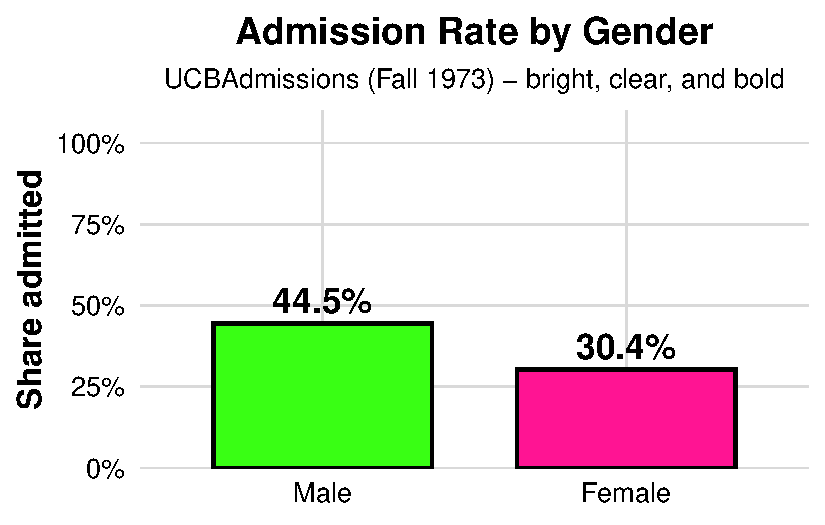
\includegraphics[keepaspectratio]{index_files/figure-pdf/unnamed-chunk-17-1.pdf}}

\subsection{Visualizing the Structure by a Simple Barplot - By
Department
Divisions}\label{visualizing-the-structure-by-a-simple-barplot---by-department-divisions}

This bra graph shows how selective each department is at UC Berkeley.
Each orange bar represents one department, and the height of the bar
indicates the percentage of applicants who were admitted. The taller the
bar, the higher the admit rate --- meaning that department is less
selective. Shorter bars show more competitive departments where fewer
applicants were admitted. The percentage label above each bar gives the
exact admit rate, making it easy to compare departments directly.
Overall, the chart gives a clear visual summary of which departments are
more or less selective in admissions.

\begin{Shaded}
\begin{Highlighting}[]
\CommentTok{\#| label: ucb{-}admit{-}bar{-}gender}
\CommentTok{\#| fig{-}width: 7}
\CommentTok{\#| fig{-}height: 4.6}
\CommentTok{\#| message: false}
\CommentTok{\#| warning: false}
 
\CommentTok{\# admitted share by department (overall, genders combined)}
\NormalTok{dept\_select }\OtherTok{\textless{}{-}} \FunctionTok{as.data.frame}\NormalTok{(}\FunctionTok{margin.table}\NormalTok{(UCBAdmissions, }\FunctionTok{c}\NormalTok{(}\DecValTok{1}\NormalTok{,}\DecValTok{3}\NormalTok{))) }\SpecialCharTok{|\textgreater{}}
  \FunctionTok{pivot\_wider}\NormalTok{(}\AttributeTok{names\_from =}\NormalTok{ Admit, }\AttributeTok{values\_from =}\NormalTok{ Freq) }\SpecialCharTok{|\textgreater{}}
  \FunctionTok{mutate}\NormalTok{(}\AttributeTok{n =}\NormalTok{ Admitted }\SpecialCharTok{+}\NormalTok{ Rejected,}
         \AttributeTok{pct =}\NormalTok{ Admitted }\SpecialCharTok{/}\NormalTok{ n)}

\FunctionTok{ggplot}\NormalTok{(dept\_select, }\FunctionTok{aes}\NormalTok{(Dept, pct)) }\SpecialCharTok{+}
  \FunctionTok{geom\_col}\NormalTok{(}\AttributeTok{width =} \FloatTok{0.70}\NormalTok{, }\AttributeTok{fill =} \StringTok{"orange"}\NormalTok{) }\SpecialCharTok{+}  \CommentTok{\# purple from your example vibe}
  \FunctionTok{geom\_text}\NormalTok{(}\FunctionTok{aes}\NormalTok{(}\AttributeTok{label =} \FunctionTok{percent}\NormalTok{(pct, }\AttributeTok{accuracy =} \FloatTok{0.1}\NormalTok{)),}
            \AttributeTok{vjust =} \SpecialCharTok{{-}}\FloatTok{0.35}\NormalTok{, }\AttributeTok{size =} \FloatTok{4.1}\NormalTok{) }\SpecialCharTok{+}
  \FunctionTok{scale\_y\_continuous}\NormalTok{(}\AttributeTok{labels =} \FunctionTok{percent\_format}\NormalTok{(),}
                     \AttributeTok{expand =} \FunctionTok{expansion}\NormalTok{(}\AttributeTok{mult =} \FunctionTok{c}\NormalTok{(}\DecValTok{0}\NormalTok{, .}\DecValTok{08}\NormalTok{))) }\SpecialCharTok{+}
  \FunctionTok{labs}\NormalTok{(}\AttributeTok{title =} \StringTok{"Department Selectivity (Admitted Share)"}\NormalTok{,}
       \AttributeTok{x =} \StringTok{"Department"}\NormalTok{, }\AttributeTok{y =} \StringTok{"Share admitted"}\NormalTok{,}
       \AttributeTok{caption =} \StringTok{"UCBAdmissions (Fall 1973)"}\NormalTok{) }\SpecialCharTok{+}
  \FunctionTok{theme\_minimal}\NormalTok{(}\AttributeTok{base\_size =} \DecValTok{12}\NormalTok{) }\SpecialCharTok{+}
  \FunctionTok{theme}\NormalTok{(}\AttributeTok{plot.title.position =} \StringTok{"plot"}\NormalTok{,}
        \AttributeTok{axis.title.y =} \FunctionTok{element\_text}\NormalTok{(}\AttributeTok{face =} \StringTok{"bold"}\NormalTok{))}
\end{Highlighting}
\end{Shaded}

\pandocbounded{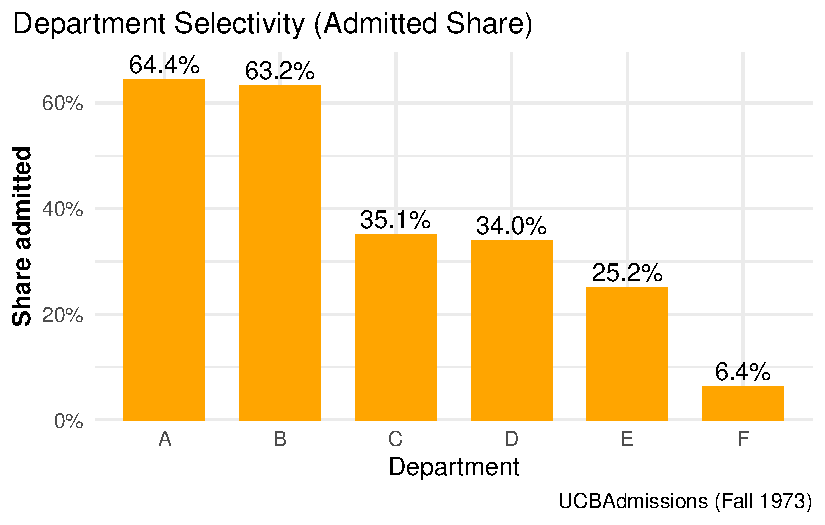
\includegraphics[keepaspectratio]{index_files/figure-pdf/unnamed-chunk-18-1.pdf}}

\subsection{Visualizing the Structure (Mosaic \& Bar
Plots)}\label{visualizing-the-structure-mosaic-bar-plots}

This figure shows a clean, comparative view of admissions outcomes
across departments and by gender, using a simple stacked bar chart. Each
bar represents one department at UC Berkeley, and the colored segments
show how many applicants were admitted versus rejected. Faceting the
chart by gender creates two panels---one for women and one for men---so
students can easily compare patterns side by side without crowding the
display.

The chart emphasizes relative shares visually: taller ``admitted''
segments mean higher success rates within that department, while smaller
ones indicate lower acceptance. By comparing across panels, you can see
whether men and women tended to be admitted at similar rates in each
department.

This kind of bar chart is one of the most intuitive ways to display
categorical outcomes, helping students connect data structure to
interpretation. It also reinforces a central lesson in social
statistics: before moving to complex models, we first use clear, direct
visuals to explore how outcomes differ across groups and institutional
contexts.

\begin{Shaded}
\begin{Highlighting}[]
\CommentTok{\# Tidy bar plot: admitted proportion by gender within department.}
\CommentTok{\# (Requires ggplot2; included if you loaded tidyverse.)}


\CommentTok{\# Load plotting and formatting helpers (percent labels).}
\FunctionTok{library}\NormalTok{(ggplot2); }\FunctionTok{library}\NormalTok{(scales)}

\CommentTok{\# Draw stacked bars per department, scaled to *proportions* (“position = \textquotesingle{}fill\textquotesingle{}”),}
\CommentTok{\# and facet the figure so Female and Male are shown in separate panels.}
\FunctionTok{ggplot}\NormalTok{(ucb, }\FunctionTok{aes}\NormalTok{(}\AttributeTok{x =}\NormalTok{ Dept, }\AttributeTok{y =}\NormalTok{ Freq, }\AttributeTok{fill =}\NormalTok{ Admit)) }\SpecialCharTok{+}
  \CommentTok{\# Stack admitted + rejected to 100\% within each Dept for each facet.}
  \FunctionTok{geom\_col}\NormalTok{(}\AttributeTok{position =} \StringTok{"fill"}\NormalTok{) }\SpecialCharTok{+}
  \CommentTok{\# One facet per Gender so we can compare shapes directly.}
  \FunctionTok{facet\_wrap}\NormalTok{(}\SpecialCharTok{\textasciitilde{}}\NormalTok{ Gender) }\SpecialCharTok{+}
  \CommentTok{\# Pretty percent labels on the y axis.}
  \FunctionTok{scale\_y\_continuous}\NormalTok{(}\AttributeTok{labels =}\NormalTok{ percent) }\SpecialCharTok{+}
  \CommentTok{\# Clear title and axis labels so readers know exactly what’s being shown.}
  \FunctionTok{labs}\NormalTok{(}\AttributeTok{title =} \StringTok{"Admission Rates by Dept, Faceted by Gender"}\NormalTok{,}
       \AttributeTok{y =} \StringTok{"Share within Dept"}\NormalTok{, }\AttributeTok{x =} \StringTok{"Department"}\NormalTok{, }\AttributeTok{fill =} \StringTok{"Decision"}\NormalTok{) }\SpecialCharTok{+}
  \CommentTok{\# Minimal theme keeps focus on the data.}
  \FunctionTok{theme\_minimal}\NormalTok{()}
\end{Highlighting}
\end{Shaded}

\pandocbounded{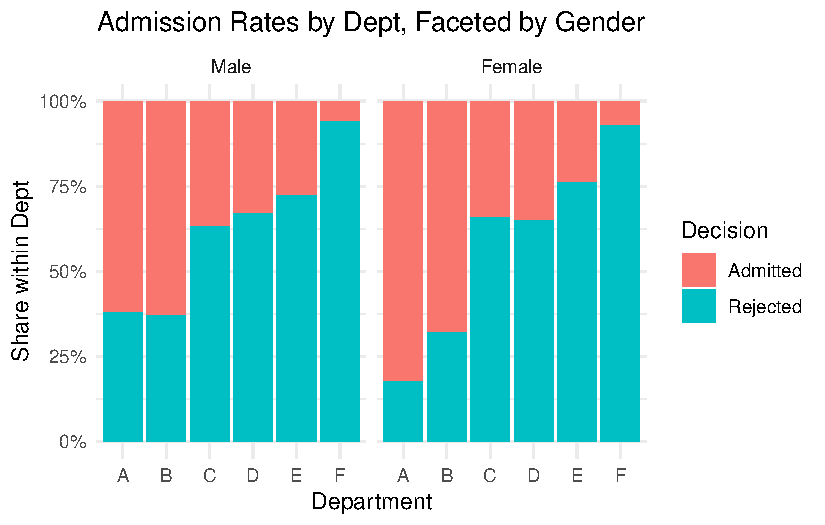
\includegraphics[keepaspectratio]{index_files/figure-pdf/unnamed-chunk-19-1.pdf}}

\subsection{More Sophisticated Way of
Visualizing}\label{more-sophisticated-way-of-visualizing}

This chart compares admission rates by gender within each department,
while also showing uncertainty. Each department appears on the x-axis
with two side-by-side (``dodged'') points: one for female and one for
male, where the point's height is the estimated admitted share in that
department. The thick vertical bars through each point are 95\%
confidence intervals from prop.test, which indicate the range of values
consistent with the data; shorter bars mean more precise estimates
(usually more applicants), and longer bars mean less precision. You may
read it as such: within a given department, compare the two points (who
is higher?) and check whether the CIs overlap (is the difference clearly
large or could it plausibly be zero?). The y-axis is in percent, capped
at 90\% to keep the comparisons visually clear. The bright colors and
large markers make the pairwise contrast obvious, but the substantive
message is about conditional comparisons (gender within department) and
uncertainty (CIs). Use this figure to teach students that headline gaps
can vanish or flip once you condition on the relevant grouping and
account for sampling variability.

\begin{Shaded}
\begin{Highlighting}[]
\CommentTok{\# Plot the Dept × Gender admitted share with gaudy colors \& bigger markers}
\FunctionTok{ggplot}\NormalTok{(dg, }\FunctionTok{aes}\NormalTok{(Dept, p\_hat, }\AttributeTok{color =}\NormalTok{ Gender)) }\SpecialCharTok{+}
  \CommentTok{\# Thick, obvious 95\% CI bars; widened dodge so points don\textquotesingle{}t overlap}
  \FunctionTok{geom\_errorbar}\NormalTok{(}\FunctionTok{aes}\NormalTok{(}\AttributeTok{ymin =}\NormalTok{ lwr, }\AttributeTok{ymax =}\NormalTok{ upr),}
                \AttributeTok{position =} \FunctionTok{position\_dodge}\NormalTok{(}\AttributeTok{width =} \FloatTok{0.6}\NormalTok{),}
                \AttributeTok{width =} \FloatTok{0.2}\NormalTok{, }\AttributeTok{linewidth =} \FloatTok{1.4}\NormalTok{) }\SpecialCharTok{+}
  \CommentTok{\# Big, loud points}
  \FunctionTok{geom\_point}\NormalTok{(}\AttributeTok{position =} \FunctionTok{position\_dodge}\NormalTok{(}\AttributeTok{width =} \FloatTok{0.6}\NormalTok{),}
             \AttributeTok{size =} \FloatTok{5.2}\NormalTok{) }\SpecialCharTok{+}
  \CommentTok{\# Percent axis}
  \FunctionTok{scale\_y\_continuous}\NormalTok{(}\AttributeTok{labels =}\NormalTok{ scales}\SpecialCharTok{::}\NormalTok{percent, }\AttributeTok{limits =} \FunctionTok{c}\NormalTok{(}\DecValTok{0}\NormalTok{, }\FloatTok{0.9}\NormalTok{),}
                     \AttributeTok{expand =} \FunctionTok{expansion}\NormalTok{(}\AttributeTok{mult =} \FunctionTok{c}\NormalTok{(}\DecValTok{0}\NormalTok{, }\FloatTok{0.03}\NormalTok{))) }\SpecialCharTok{+}
  \CommentTok{\# Neon, high{-}contrast palette}
  \FunctionTok{scale\_color\_manual}\NormalTok{(}\AttributeTok{values =} \FunctionTok{c}\NormalTok{(}
    \StringTok{"Female"} \OtherTok{=} \StringTok{"\#FF1493"}\NormalTok{,  }\CommentTok{\# deep magenta / neon pink}
    \StringTok{"Male"}   \OtherTok{=} \StringTok{"\#39FF14"}   \CommentTok{\# neon green}
\NormalTok{  )) }\SpecialCharTok{+}
  \FunctionTok{labs}\NormalTok{(}\AttributeTok{title =} \StringTok{"UC Berkeley Admissions by Dept × Gender"}\NormalTok{,}
       \AttributeTok{subtitle =} \StringTok{"Point = admitted share; line = 95\% CI (prop.test)"}\NormalTok{,}
       \AttributeTok{x =} \StringTok{"Department"}\NormalTok{, }\AttributeTok{y =} \StringTok{"Admitted (\%)"}\NormalTok{, }\AttributeTok{color =} \StringTok{"Gender"}\NormalTok{) }\SpecialCharTok{+}
  \CommentTok{\# Make legend keys big enough to match the jumbo points}
  \FunctionTok{guides}\NormalTok{(}\AttributeTok{color =} \FunctionTok{guide\_legend}\NormalTok{(}\AttributeTok{override.aes =} \FunctionTok{list}\NormalTok{(}\AttributeTok{size =} \DecValTok{5}\NormalTok{)))  }\SpecialCharTok{+} \FunctionTok{theme\_classic}\NormalTok{()}
\end{Highlighting}
\end{Shaded}

\pandocbounded{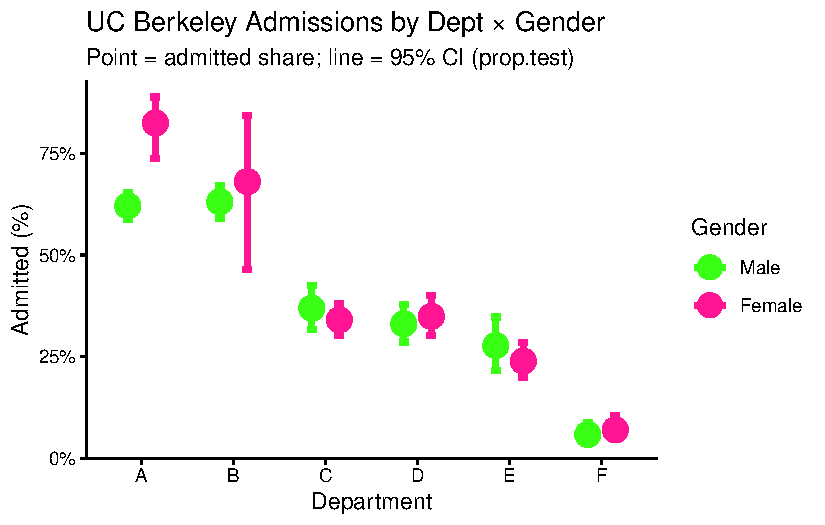
\includegraphics[keepaspectratio]{index_files/figure-pdf/unnamed-chunk-20-1.pdf}}

\section{Even A More Sophisticated Way of
Visualization}\label{even-a-more-sophisticated-way-of-visualization}

This figure shows how admission rates are distributed across departments
for each gender, not just a single average. The wide, smooth violin
shapes trace the full distribution of department-level admit
rates---thicker sections mean more departments fall in that range,
thinner sections mean fewer. Over the violin, the boxplot adds quick
landmarks: the box spans the interquartile range (IQR) where the middle
50\% of departments lie, and the line inside the box marks the median.
To make that median impossible to miss, a large yellow dot is plotted
right on it. Reading the plot is straightforward: compare the height and
thickness of the two violins to see differences in spread and typical
values, and compare the median dots to see which gender tends to have
higher rates across departments. Because the y-axis is in percent and
capped at 90\%, the common range is easy to scan without squashing the
detail. Use this plot when you want students to see distributional
differences (center and spread) across groups, not just their means.

\begin{Shaded}
\begin{Highlighting}[]
\CommentTok{\# Compare the *distribution* of department{-}level admitted shares by gender:}
\CommentTok{\# violin = overall shape; box = IQR; black dot = median.}
\FunctionTok{ggplot}\NormalTok{(dg, }\FunctionTok{aes}\NormalTok{(Gender, p\_hat, }\AttributeTok{fill =}\NormalTok{ Gender)) }\SpecialCharTok{+}
  \CommentTok{\# Smooth density shape of dept{-}level rates per gender.}
  \FunctionTok{geom\_violin}\NormalTok{(}\AttributeTok{alpha =} \FloatTok{0.8}\NormalTok{, }\AttributeTok{color =} \ConstantTok{NA}\NormalTok{, }\AttributeTok{width =} \FloatTok{0.9}\NormalTok{) }\SpecialCharTok{+}
  \CommentTok{\# Boxplot overlay shows median + IQR without outliers drawn.}
  \FunctionTok{geom\_boxplot}\NormalTok{(}\AttributeTok{width =} \FloatTok{0.15}\NormalTok{, }\AttributeTok{fill =} \StringTok{"white"}\NormalTok{, }\AttributeTok{outlier.shape =} \ConstantTok{NA}\NormalTok{) }\SpecialCharTok{+}
  \CommentTok{\# Add a dot at the median for quick comparison.}
   \FunctionTok{stat\_summary}\NormalTok{(}\AttributeTok{fun =}\NormalTok{ median, }\AttributeTok{geom =} \StringTok{"point"}\NormalTok{, }\AttributeTok{size =} \DecValTok{6}\NormalTok{,}
               \AttributeTok{shape =} \DecValTok{21}\NormalTok{, }\AttributeTok{stroke =} \FloatTok{1.3}\NormalTok{, }\AttributeTok{color =} \StringTok{"black"}\NormalTok{,}
               \AttributeTok{fill =} \StringTok{"\#FFFF00"}\NormalTok{) }\SpecialCharTok{+}
  \CommentTok{\# Percent axis, clipped to [0, 0.9] with a little visual breathing room.}
  \FunctionTok{scale\_y\_continuous}\NormalTok{(}\AttributeTok{labels =} \FunctionTok{percent\_format}\NormalTok{(}\AttributeTok{accuracy =} \DecValTok{1}\NormalTok{),}
                     \AttributeTok{limits =} \FunctionTok{c}\NormalTok{(}\DecValTok{0}\NormalTok{, }\FloatTok{0.9}\NormalTok{),}
                     \AttributeTok{expand =} \FunctionTok{expansion}\NormalTok{(}\AttributeTok{mult =} \FunctionTok{c}\NormalTok{(}\DecValTok{0}\NormalTok{, .}\DecValTok{03}\NormalTok{))) }\SpecialCharTok{+}
  \CommentTok{\# Manually set fills so the palette matches prior plots.}
  \FunctionTok{scale\_fill\_manual}\NormalTok{(}\AttributeTok{values =} \FunctionTok{c}\NormalTok{(}\StringTok{"Female"} \OtherTok{=} \StringTok{"\#FF1493"}\NormalTok{, }\StringTok{"Male"} \OtherTok{=} \StringTok{"\#39FF14"}\NormalTok{)) }\SpecialCharTok{+}
  \CommentTok{\# Title/subtitle clarify what each glyph represents.}
  \FunctionTok{labs}\NormalTok{(}\AttributeTok{title =} \StringTok{"Distribution of Department{-}Level Admit Rates"}\NormalTok{,}
       \AttributeTok{subtitle =} \StringTok{"Each violin = spread of departments; dot = median"}\NormalTok{,}
       \AttributeTok{x =} \ConstantTok{NULL}\NormalTok{, }\AttributeTok{y =} \StringTok{"Admitted (\%)"}\NormalTok{) }\SpecialCharTok{+}
  \CommentTok{\# Clean theme, slightly larger base text, and hide redundant legend.}
  \FunctionTok{theme\_minimal}\NormalTok{(}\AttributeTok{base\_size =} \DecValTok{13}\NormalTok{) }\SpecialCharTok{+}
  \FunctionTok{theme}\NormalTok{(}\AttributeTok{legend.position =} \StringTok{"none"}\NormalTok{,}
        \AttributeTok{plot.title.position =} \StringTok{"plot"}\NormalTok{)}
\end{Highlighting}
\end{Shaded}

\pandocbounded{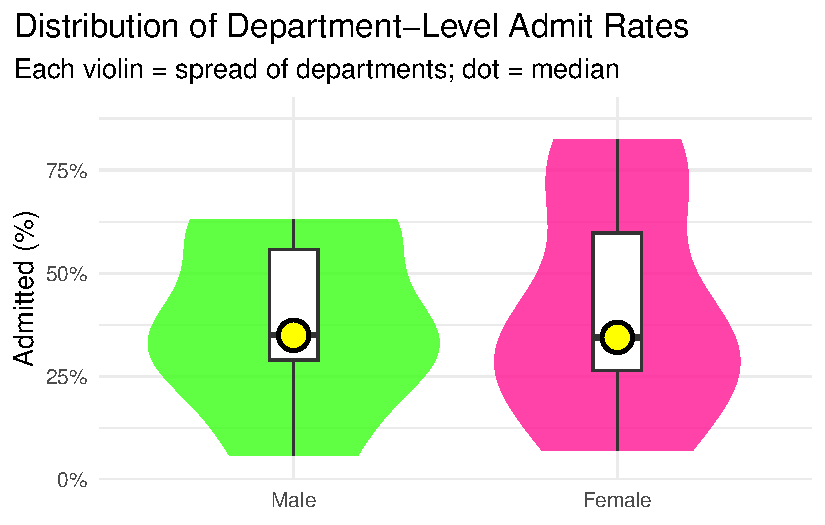
\includegraphics[keepaspectratio]{index_files/figure-pdf/unnamed-chunk-21-1.pdf}}

\section{Visualization Faceted by Department at UC
Berkeley}\label{visualization-faceted-by-department-at-uc-berkeley}

This plot helps us visualize gender differences in admission rates
within each department. We start by reshaping the data so that each
department has one column for the female admission rate and one for the
male admission rate. This ``wide'' format makes it easy to connect each
department's two values with a line.

Each line links the female rate (on the left) to the male rate (on the
right), showing at a glance which gender had the higher admission rate
within that department. The slope and direction of the line are what
matter: if the line tilts upward to the right, men were admitted at a
higher rate; if it tilts downward, women were admitted at a higher rate.
The bright neon colors and bold points make the contrast unmistakable.
Faceting the plot by department creates one small panel per department,
so you can compare patterns across them without clutter. The x-axis
simply labels ``Female'' and ``Male,'' while the y-axis shows the
percent admitted. In short, this figure teaches a key skill in data
visualization: how to display paired comparisons across categories while
preserving the structure of the data. Each line tells its own small
story about one department---and together, they reveal the broader
pattern behind the Simpson's paradox in UC Berkeley admissions.

\begin{Shaded}
\begin{Highlighting}[]
\NormalTok{ dg\_wide }\OtherTok{\textless{}{-}}\NormalTok{ dg }\SpecialCharTok{|\textgreater{}}
  \FunctionTok{select}\NormalTok{(Dept, Gender, p\_hat) }\SpecialCharTok{|\textgreater{}}
  \FunctionTok{pivot\_wider}\NormalTok{(}\AttributeTok{names\_from =}\NormalTok{ Gender, }\AttributeTok{values\_from =}\NormalTok{ p\_hat) }\SpecialCharTok{|\textgreater{}}
  \FunctionTok{drop\_na}\NormalTok{()}


\FunctionTok{ggplot}\NormalTok{(dg\_wide) }\SpecialCharTok{+}
  \CommentTok{\# Fat, neon connector lines per department}
  \FunctionTok{geom\_segment}\NormalTok{(}\FunctionTok{aes}\NormalTok{(}\AttributeTok{x =} \DecValTok{1}\NormalTok{, }\AttributeTok{xend =} \DecValTok{2}\NormalTok{, }\AttributeTok{y =}\NormalTok{ Female, }\AttributeTok{yend =}\NormalTok{ Male),}
               \AttributeTok{color =} \StringTok{"\#00FFFF"}\NormalTok{, }\AttributeTok{linewidth =} \FloatTok{1.8}\NormalTok{, }\AttributeTok{lineend =} \StringTok{"round"}\NormalTok{, }\AttributeTok{na.rm =} \ConstantTok{TRUE}\NormalTok{) }\SpecialCharTok{+}
  \CommentTok{\# Female endpoint (left) — jumbo neon pink with black outline}
  \FunctionTok{geom\_point}\NormalTok{(}\FunctionTok{aes}\NormalTok{(}\AttributeTok{x =} \DecValTok{1}\NormalTok{, }\AttributeTok{y =}\NormalTok{ Female),}
             \AttributeTok{shape =} \DecValTok{21}\NormalTok{, }\AttributeTok{size =} \FloatTok{6.5}\NormalTok{, }\AttributeTok{stroke =} \FloatTok{1.2}\NormalTok{,}
             \AttributeTok{fill =} \StringTok{"\#FF1493"}\NormalTok{, }\AttributeTok{color =} \StringTok{"black"}\NormalTok{, }\AttributeTok{na.rm =} \ConstantTok{TRUE}\NormalTok{) }\SpecialCharTok{+}
  \CommentTok{\# Male endpoint (right) — jumbo neon green with black outline}
  \FunctionTok{geom\_point}\NormalTok{(}\FunctionTok{aes}\NormalTok{(}\AttributeTok{x =} \DecValTok{2}\NormalTok{, }\AttributeTok{y =}\NormalTok{ Male),}
             \AttributeTok{shape =} \DecValTok{21}\NormalTok{, }\AttributeTok{size =} \FloatTok{6.5}\NormalTok{, }\AttributeTok{stroke =} \FloatTok{1.2}\NormalTok{,}
             \AttributeTok{fill =} \StringTok{"\#39FF14"}\NormalTok{, }\AttributeTok{color =} \StringTok{"black"}\NormalTok{, }\AttributeTok{na.rm =} \ConstantTok{TRUE}\NormalTok{) }\SpecialCharTok{+}

  \CommentTok{\# Zoom without dropping rows}
  \FunctionTok{coord\_cartesian}\NormalTok{(}\AttributeTok{ylim =} \FunctionTok{c}\NormalTok{(}\DecValTok{0}\NormalTok{, }\FloatTok{0.90}\NormalTok{)) }\SpecialCharTok{+}

  \CommentTok{\# Two labeled x positions with extra breathing room}
  \FunctionTok{scale\_x\_continuous}\NormalTok{(}\AttributeTok{breaks =} \FunctionTok{c}\NormalTok{(}\DecValTok{1}\NormalTok{, }\DecValTok{2}\NormalTok{), }\AttributeTok{labels =} \FunctionTok{c}\NormalTok{(}\StringTok{"Female"}\NormalTok{, }\StringTok{"Male"}\NormalTok{),}
                     \AttributeTok{expand =} \FunctionTok{expansion}\NormalTok{(}\AttributeTok{add =} \FloatTok{0.25}\NormalTok{)) }\SpecialCharTok{+}
  \CommentTok{\# Percent labels for y}
  \FunctionTok{scale\_y\_continuous}\NormalTok{(}\AttributeTok{labels =} \FunctionTok{percent\_format}\NormalTok{(}\AttributeTok{accuracy =} \DecValTok{1}\NormalTok{)) }\SpecialCharTok{+}

  \CommentTok{\# One panel per department}
  \FunctionTok{facet\_wrap}\NormalTok{(}\SpecialCharTok{\textasciitilde{}}\NormalTok{ Dept, }\AttributeTok{nrow =} \DecValTok{2}\NormalTok{) }\SpecialCharTok{+}

  \CommentTok{\# {-}{-}{-} Keep your original descriptive text exactly {-}{-}{-}}
  \FunctionTok{labs}\NormalTok{(}\AttributeTok{title =} \StringTok{"Within{-}Department Admission Rates"}\NormalTok{,}
       \AttributeTok{x =} \ConstantTok{NULL}\NormalTok{, }\AttributeTok{y =} \StringTok{"Admitted (\%)"}\NormalTok{) }\SpecialCharTok{+}

  \CommentTok{\# Gaudy{-}friendly theme tweaks with centered title}
  \FunctionTok{theme\_minimal}\NormalTok{(}\AttributeTok{base\_size =} \DecValTok{16}\NormalTok{) }\SpecialCharTok{+}
  \FunctionTok{theme}\NormalTok{(}
    \AttributeTok{legend.position =} \StringTok{"none"}\NormalTok{,}
    \AttributeTok{plot.title.position =} \StringTok{"plot"}\NormalTok{,}
    \AttributeTok{plot.title =} \FunctionTok{element\_text}\NormalTok{(}\AttributeTok{face =} \StringTok{"bold"}\NormalTok{, }\AttributeTok{hjust =} \FloatTok{0.5}\NormalTok{),   }\CommentTok{\# Center title}
    \AttributeTok{plot.subtitle =} \FunctionTok{element\_text}\NormalTok{(}\AttributeTok{hjust =} \FloatTok{0.5}\NormalTok{),               }\CommentTok{\# Center subtitle}
    \AttributeTok{axis.title.y =} \FunctionTok{element\_text}\NormalTok{(}\AttributeTok{face =} \StringTok{"bold"}\NormalTok{),}
    \AttributeTok{panel.grid.major =} \FunctionTok{element\_line}\NormalTok{(}\AttributeTok{linewidth =} \FloatTok{0.4}\NormalTok{, }\AttributeTok{color =} \StringTok{"grey80"}\NormalTok{),}
    \AttributeTok{panel.grid.minor =} \FunctionTok{element\_blank}\NormalTok{(),}
    \AttributeTok{strip.text =} \FunctionTok{element\_text}\NormalTok{(}\AttributeTok{face =} \StringTok{"bold"}\NormalTok{, }\AttributeTok{color =} \StringTok{"white"}\NormalTok{),}
    \AttributeTok{strip.background =} \FunctionTok{element\_rect}\NormalTok{(}\AttributeTok{fill =} \StringTok{"black"}\NormalTok{, }\AttributeTok{color =} \ConstantTok{NA}\NormalTok{)}
\NormalTok{  )}
\end{Highlighting}
\end{Shaded}

\pandocbounded{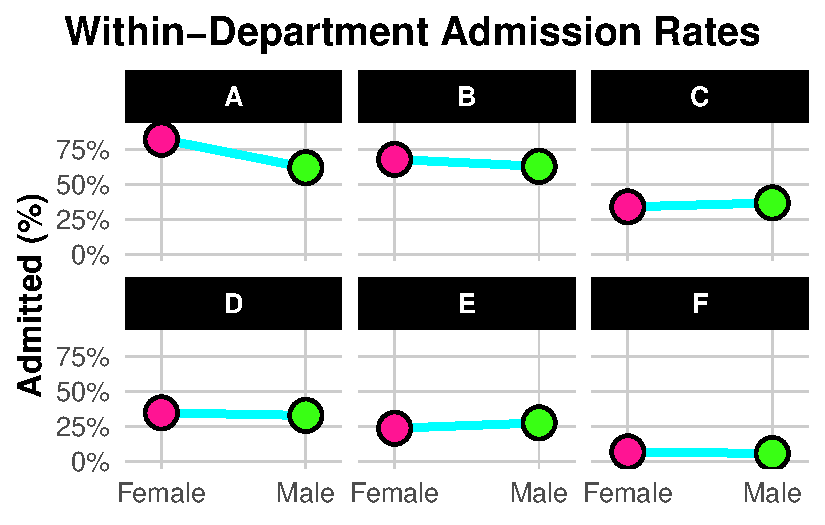
\includegraphics[keepaspectratio]{index_files/figure-pdf/unnamed-chunk-22-1.pdf}}

\section{Selecting Appropriate Graphical
Summaries}\label{selecting-appropriate-graphical-summaries}

\begin{itemize}
\tightlist
\item
  \textbf{Quantitative}: \textbf{histograms/box plots} (large n);
  \textbf{dot plots} (small n).\\
\item
  \textbf{Categorical}: \textbf{bar charts} or \textbf{frequency
  tables}; pie charts only when categories are few and distinct.\\
\item
  \textbf{Two quantitative}: \textbf{scatterplot}.\\
\item
  \textbf{One quantitative across groups}: \textbf{box/violin}.\\
\item
  \textbf{Categorical across groups}: \textbf{contingency/mosaic}.
\end{itemize}

\section{A Small, Reproducible Example
Dataset}\label{a-small-reproducible-example-dataset}

\begin{Shaded}
\begin{Highlighting}[]
\NormalTok{n }\OtherTok{\textless{}{-}} \DecValTok{600}
\NormalTok{ps }\OtherTok{\textless{}{-}} \FunctionTok{tibble}\NormalTok{(}
  \AttributeTok{respondent =} \DecValTok{1}\SpecialCharTok{:}\NormalTok{n,}
  \AttributeTok{state =} \FunctionTok{sample}\NormalTok{(state.abb, n, }\ConstantTok{TRUE}\NormalTok{),}
  \AttributeTok{party =} \FunctionTok{fct\_infreq}\NormalTok{(}\FunctionTok{sample}\NormalTok{(}\FunctionTok{c}\NormalTok{(}\StringTok{"Democrat"}\NormalTok{,}\StringTok{"Independent"}\NormalTok{,}\StringTok{"Republican"}\NormalTok{), n, }\ConstantTok{TRUE}\NormalTok{, }\AttributeTok{prob =} \FunctionTok{c}\NormalTok{(.}\DecValTok{36}\NormalTok{,.}\DecValTok{28}\NormalTok{,.}\DecValTok{36}\NormalTok{))),}
  \AttributeTok{ideology =} \FunctionTok{rnorm}\NormalTok{(n, }\AttributeTok{mean =} \FunctionTok{ifelse}\NormalTok{(party}\SpecialCharTok{==}\StringTok{"Democrat"}\NormalTok{,}\SpecialCharTok{{-}}\FloatTok{0.2}\NormalTok{, }\FunctionTok{ifelse}\NormalTok{(party}\SpecialCharTok{==}\StringTok{"Republican"}\NormalTok{,}\FloatTok{0.3}\NormalTok{,}\DecValTok{0}\NormalTok{)), }\AttributeTok{sd =} \FloatTok{0.9}\NormalTok{),}
  \AttributeTok{turnout =} \FunctionTok{pmin}\NormalTok{(}\FunctionTok{pmax}\NormalTok{(}\FunctionTok{round}\NormalTok{(}\FunctionTok{rbeta}\NormalTok{(n, }\DecValTok{5}\NormalTok{, }\DecValTok{3}\NormalTok{) }\SpecialCharTok{*} \DecValTok{100}\NormalTok{), }\DecValTok{0}\NormalTok{), }\DecValTok{100}\NormalTok{),}
  \AttributeTok{income\_thou =} \FunctionTok{round}\NormalTok{(}\FunctionTok{rlnorm}\NormalTok{(n, }\FunctionTok{log}\NormalTok{(}\DecValTok{60}\NormalTok{), }\FloatTok{0.45}\NormalTok{)),}
  \AttributeTok{incumbent\_contact =} \FunctionTok{rbinom}\NormalTok{(n, }\DecValTok{1}\NormalTok{, }\FunctionTok{ifelse}\NormalTok{(party}\SpecialCharTok{==}\StringTok{"Democrat"}\NormalTok{, .}\DecValTok{52}\NormalTok{, .}\DecValTok{48}\NormalTok{)),}
  \AttributeTok{method =} \FunctionTok{sample}\NormalTok{(}\FunctionTok{c}\NormalTok{(}\StringTok{"Door{-}to{-}Door"}\NormalTok{,}\StringTok{"Phone"}\NormalTok{), n, }\ConstantTok{TRUE}\NormalTok{, }\AttributeTok{prob =} \FunctionTok{c}\NormalTok{(.}\DecValTok{55}\NormalTok{,.}\DecValTok{45}\NormalTok{)),}
  \AttributeTok{donation =} \FunctionTok{round}\NormalTok{(}\FunctionTok{rlnorm}\NormalTok{(n, }\FunctionTok{log}\NormalTok{(}\DecValTok{200}\NormalTok{), }\FloatTok{1.1}\NormalTok{))}
\NormalTok{)}
\FunctionTok{summary}\NormalTok{(ps)}
\end{Highlighting}
\end{Shaded}

\begin{verbatim}
   respondent       state                   party        ideology       
 Min.   :  1.0   Length:600         Democrat   :225   Min.   :-2.75901  
 1st Qu.:150.8   Class :character   Republican :223   1st Qu.:-0.59832  
 Median :300.5   Mode  :character   Independent:152   Median : 0.01644  
 Mean   :300.5                                        Mean   : 0.01598  
 3rd Qu.:450.2                                        3rd Qu.: 0.62120  
 Max.   :600.0                                        Max.   : 2.70922  
    turnout       income_thou     incumbent_contact    method         
 Min.   :21.00   Min.   : 17.00   Min.   :0.0       Length:600        
 1st Qu.:51.75   1st Qu.: 43.00   1st Qu.:0.0       Class :character  
 Median :64.00   Median : 59.50   Median :0.5       Mode  :character  
 Mean   :62.98   Mean   : 64.51   Mean   :0.5                         
 3rd Qu.:75.00   3rd Qu.: 80.25   3rd Qu.:1.0                         
 Max.   :97.00   Max.   :216.00   Max.   :1.0                         
    donation      
 Min.   :    6.0  
 1st Qu.:  105.0  
 Median :  212.0  
 Mean   :  383.8  
 3rd Qu.:  426.2  
 Max.   :11138.0  
\end{verbatim}

\subsection{Party Identification}\label{party-identification}

This bar chart summarizes a categorical variable by displaying the share
of respondents in each party category. Heights encode proportions
(y-axis in percent), and direct labels above the bars make exact values
easy to read without consulting the axis. Because bars compare parts of
a whole, the figure immediately communicates relative size (e.g.,
whether Democrats and Republicans are similarly common and how
Independents compare). This is the preferred display for nominal
categories; pies are harder to compare precisely, and frequency tables
lack visual punch. Interpretation is purely descriptive---no uncertainty
bands are shown---so readers should treat the reported shares as sample
estimates that would vary across samples.

\begin{Shaded}
\begin{Highlighting}[]
\NormalTok{party\_share }\OtherTok{\textless{}{-}}\NormalTok{ ps }\SpecialCharTok{|\textgreater{}} \FunctionTok{count}\NormalTok{(party) }\SpecialCharTok{|\textgreater{}} \FunctionTok{mutate}\NormalTok{(}\AttributeTok{pct =}\NormalTok{ n}\SpecialCharTok{/}\FunctionTok{sum}\NormalTok{(n))}
\NormalTok{party\_share }\SpecialCharTok{|\textgreater{}}
  \FunctionTok{ggplot}\NormalTok{(}\FunctionTok{aes}\NormalTok{(party, pct, }\AttributeTok{fill =}\NormalTok{ party)) }\SpecialCharTok{+}
  \FunctionTok{geom\_col}\NormalTok{(}\AttributeTok{width =} \FloatTok{0.7}\NormalTok{, }\AttributeTok{show.legend =} \ConstantTok{FALSE}\NormalTok{) }\SpecialCharTok{+}
  \FunctionTok{geom\_text}\NormalTok{(}\FunctionTok{aes}\NormalTok{(}\AttributeTok{label =} \FunctionTok{percent}\NormalTok{(pct, .}\DecValTok{1}\NormalTok{)), }\AttributeTok{vjust =} \SpecialCharTok{{-}}\FloatTok{0.3}\NormalTok{, }\AttributeTok{size =} \FloatTok{4.1}\NormalTok{) }\SpecialCharTok{+}
  \FunctionTok{scale\_y\_continuous}\NormalTok{(}\AttributeTok{labels =} \FunctionTok{percent\_format}\NormalTok{(), }\AttributeTok{expand =} \FunctionTok{expansion}\NormalTok{(}\AttributeTok{mult =} \FunctionTok{c}\NormalTok{(}\DecValTok{0}\NormalTok{, .}\DecValTok{08}\NormalTok{))) }\SpecialCharTok{+}
  \FunctionTok{scale\_fill\_manual}\NormalTok{(}\AttributeTok{values =}\NormalTok{ pol\_pal) }\SpecialCharTok{+}
  \FunctionTok{labs}\NormalTok{(}\AttributeTok{title =} \StringTok{"Party Identification of Respondents"}\NormalTok{, }\AttributeTok{x =} \ConstantTok{NULL}\NormalTok{, }\AttributeTok{y =} \StringTok{"Share of sample"}\NormalTok{,}
       \AttributeTok{caption =} \StringTok{"Simulated data (Soc 108)"}\NormalTok{)}
\end{Highlighting}
\end{Shaded}

\pandocbounded{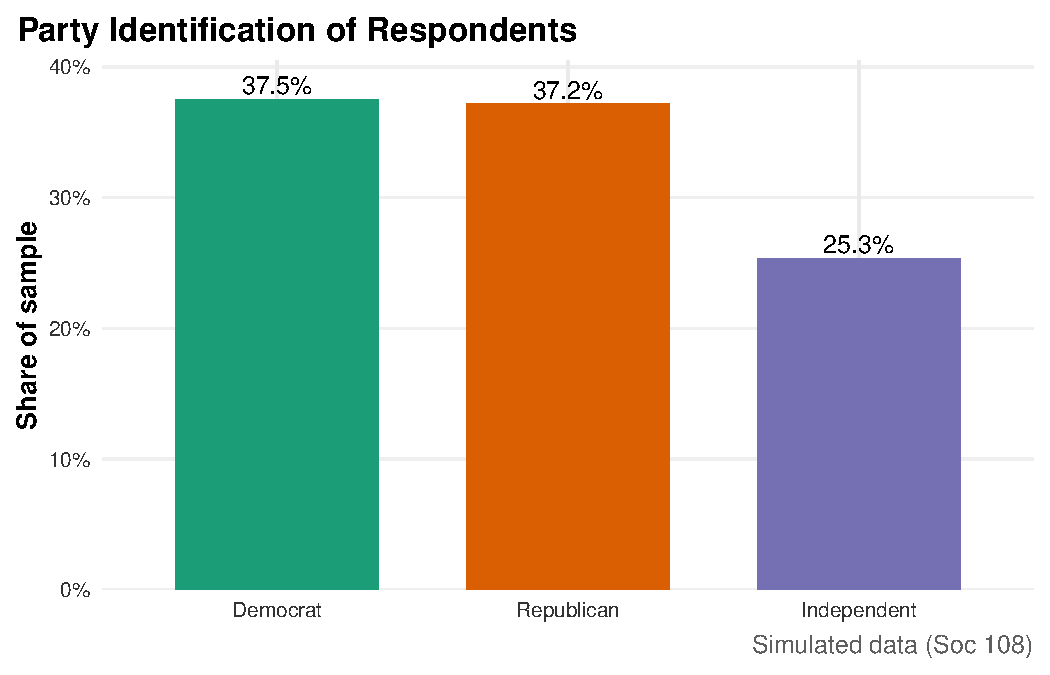
\includegraphics[keepaspectratio]{index_files/figure-pdf/ch1-party-1.pdf}}

\subsection{Turnout Distribution}\label{turnout-distribution}

The histogram describes the distribution of a quantitative variable
(self-reported turnout as a percentage). Bins partition the scale into
intervals; bar area reflects relative frequency (using density on the
y-axis so the total area integrates to 1). The vertical solid and dashed
lines mark the mean and median, respectively, making skew and outliers
visible at a glance (when the two lines separate, the distribution is
asymmetric). The chosen bin count balances smoothness and granularity;
too few bins hide structure, too many add noise. This plot is ideal for
discussing central tendency, spread, and shape before moving to formal
statistics.

\begin{Shaded}
\begin{Highlighting}[]
\NormalTok{m }\OtherTok{\textless{}{-}} \FunctionTok{mean}\NormalTok{(ps}\SpecialCharTok{$}\NormalTok{turnout); md }\OtherTok{\textless{}{-}} \FunctionTok{median}\NormalTok{(ps}\SpecialCharTok{$}\NormalTok{turnout)}
\NormalTok{ps }\SpecialCharTok{|\textgreater{}}
  \FunctionTok{ggplot}\NormalTok{(}\FunctionTok{aes}\NormalTok{(turnout)) }\SpecialCharTok{+}
  \FunctionTok{geom\_histogram}\NormalTok{(}\FunctionTok{aes}\NormalTok{(}\AttributeTok{y =} \FunctionTok{after\_stat}\NormalTok{(density)), }\AttributeTok{bins =} \DecValTok{25}\NormalTok{, }\AttributeTok{boundary =} \DecValTok{0}\NormalTok{,}
                 \AttributeTok{color =} \StringTok{"white"}\NormalTok{, }\AttributeTok{fill =}\NormalTok{ pol\_pal[}\DecValTok{3}\NormalTok{]) }\SpecialCharTok{+}
  \FunctionTok{geom\_vline}\NormalTok{(}\AttributeTok{xintercept =}\NormalTok{ m) }\SpecialCharTok{+}
  \FunctionTok{geom\_vline}\NormalTok{(}\AttributeTok{xintercept =}\NormalTok{ md, }\AttributeTok{linetype =} \DecValTok{2}\NormalTok{) }\SpecialCharTok{+}
  \FunctionTok{annotate}\NormalTok{(}\StringTok{"label"}\NormalTok{, }\AttributeTok{x =}\NormalTok{ m,  }\AttributeTok{y =} \FloatTok{0.02}\NormalTok{,  }\AttributeTok{label =} \FunctionTok{glue}\NormalTok{(}\StringTok{"Mean = \{round(m,1)\}\%"}\NormalTok{)) }\SpecialCharTok{+}
  \FunctionTok{annotate}\NormalTok{(}\StringTok{"label"}\NormalTok{, }\AttributeTok{x =}\NormalTok{ md, }\AttributeTok{y =} \FloatTok{0.018}\NormalTok{, }\AttributeTok{label =} \FunctionTok{glue}\NormalTok{(}\StringTok{"Median = \{round(md,1)\}\%"}\NormalTok{)) }\SpecialCharTok{+}
  \FunctionTok{labs}\NormalTok{(}\AttributeTok{title =} \StringTok{"Distribution of Self{-}Reported Turnout"}\NormalTok{,}
       \AttributeTok{subtitle =} \StringTok{"Solid = mean; dashed = median"}\NormalTok{,}
       \AttributeTok{x =} \StringTok{"Percent"}\NormalTok{, }\AttributeTok{y =} \StringTok{"Density"}\NormalTok{,}
       \AttributeTok{caption =} \StringTok{"Simulated data (Soc 108)"}\NormalTok{)}
\end{Highlighting}
\end{Shaded}

\pandocbounded{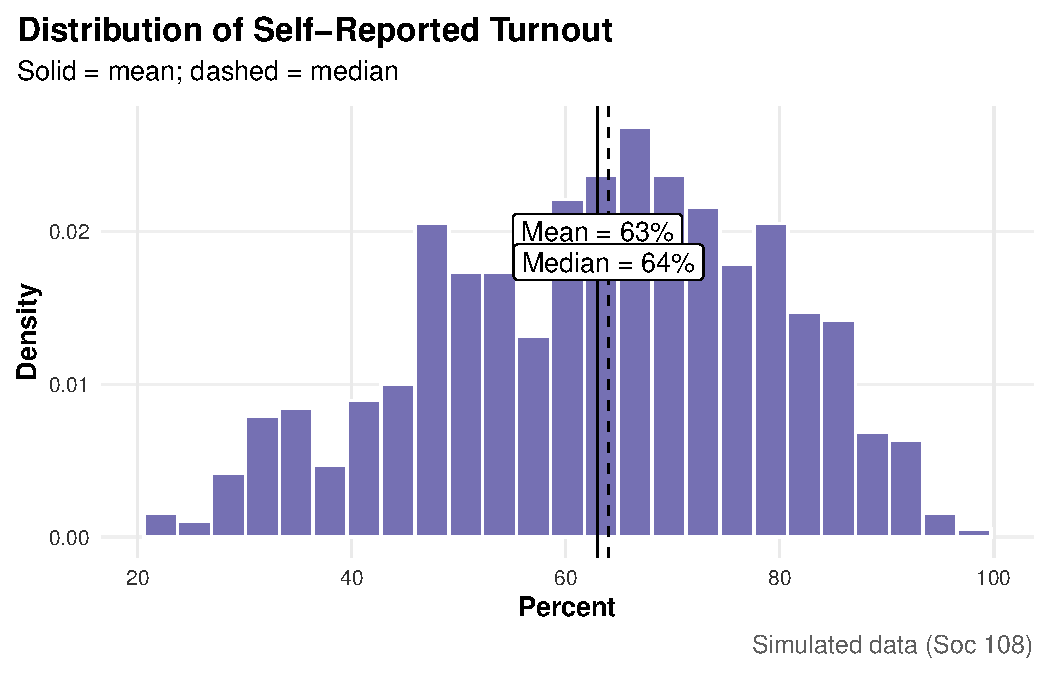
\includegraphics[keepaspectratio]{index_files/figure-pdf/ch1-turnout-1.pdf}}

\subsection{Inequality vs Turnout}\label{inequality-vs-turnout}

This scatterplot examines the relationship between two quantitative
variables---a simulated county Gini index (x) and turnout (y). Each
point is a unit; the semi-transparent dots reduce overplotting in dense
regions. The LOESS curve provides a nonparametric trend with a shaded
confidence band, revealing possible curvature without assuming a
particular functional form. The x-axis is formatted as percentages to
match the Gini scale. Because this is observational, the figure supports
association, not causation; it is best used to motivate model choice
(e.g., whether a linear, quadratic, or spline term is appropriate).

\begin{Shaded}
\begin{Highlighting}[]
\NormalTok{ps2 }\OtherTok{\textless{}{-}}\NormalTok{ ps }\SpecialCharTok{|\textgreater{}} \FunctionTok{mutate}\NormalTok{(}\AttributeTok{gini =} \FunctionTok{pmin}\NormalTok{(}\FunctionTok{pmax}\NormalTok{(}\FunctionTok{rnorm}\NormalTok{(}\FunctionTok{n}\NormalTok{(), }\FloatTok{0.43}\NormalTok{, }\FloatTok{0.05}\NormalTok{), }\FloatTok{0.30}\NormalTok{), }\FloatTok{0.60}\NormalTok{))}
\NormalTok{ps2 }\SpecialCharTok{|\textgreater{}}
  \FunctionTok{ggplot}\NormalTok{(}\FunctionTok{aes}\NormalTok{(gini, turnout)) }\SpecialCharTok{+}
  \FunctionTok{geom\_point}\NormalTok{(}\AttributeTok{alpha =} \FloatTok{0.35}\NormalTok{, }\AttributeTok{size =} \FloatTok{1.5}\NormalTok{, }\AttributeTok{colour =} \StringTok{"red"}\NormalTok{) }\SpecialCharTok{+}
  \FunctionTok{geom\_smooth}\NormalTok{(}\AttributeTok{method =} \StringTok{"lm"}\NormalTok{, }\AttributeTok{se =} \ConstantTok{TRUE}\NormalTok{, }\AttributeTok{colour =} \StringTok{"blue"}\NormalTok{) }\SpecialCharTok{+}
  \FunctionTok{scale\_x\_continuous}\NormalTok{(}\AttributeTok{labels =} \FunctionTok{percent\_format}\NormalTok{(}\AttributeTok{accuracy =} \DecValTok{1}\NormalTok{)) }\SpecialCharTok{+}
  \FunctionTok{labs}\NormalTok{(}\AttributeTok{title =} \StringTok{"Higher Inequality, Lower Turnout?"}\NormalTok{,}
       \AttributeTok{subtitle =} \StringTok{"LOESS highlights possible nonlinearity"}\NormalTok{,}
       \AttributeTok{x =} \StringTok{"Gini (inequality)"}\NormalTok{, }\AttributeTok{y =} \StringTok{"Turnout (\%)"}\NormalTok{,}
       \AttributeTok{caption =} \StringTok{"Simulated data (Soc 108)"}\NormalTok{) }\SpecialCharTok{+} \FunctionTok{theme\_classic}\NormalTok{()}
\end{Highlighting}
\end{Shaded}

\pandocbounded{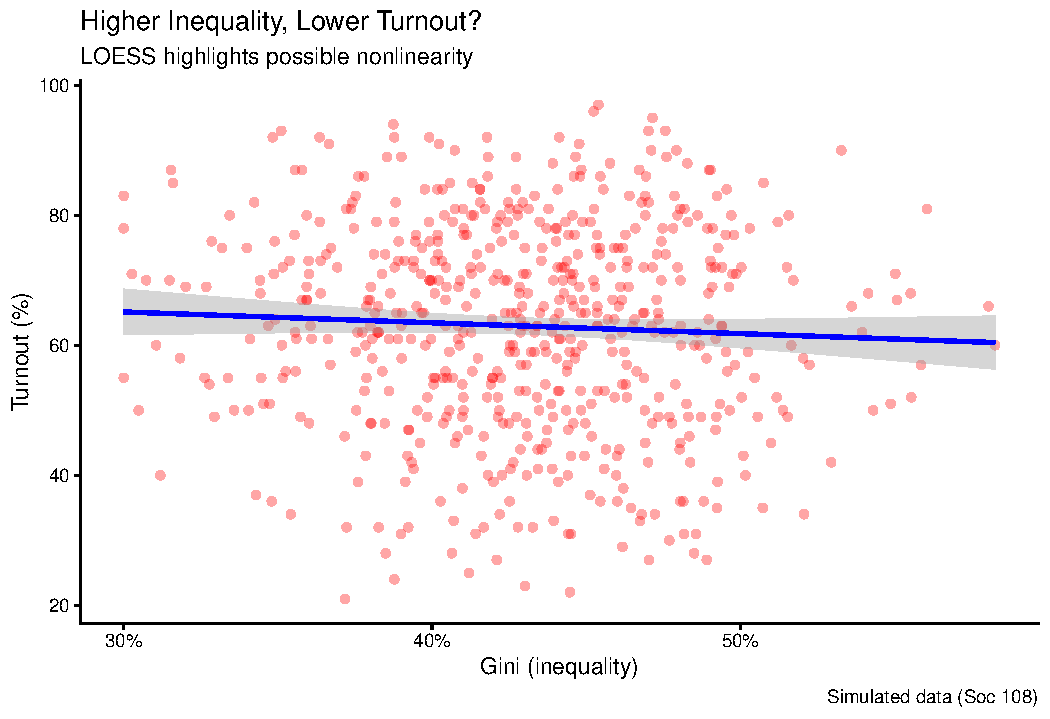
\includegraphics[keepaspectratio]{index_files/figure-pdf/ch1-ineq-1.pdf}}

\subsection{Donations by Party}\label{donations-by-party}

This figure compares a quantitative outcome across groups by combining a
violin (smoothed distribution), a boxplot (median and IQR), and a median
point overlay. The design shows both typical values and distributional
shape, which is crucial for right-skewed variables like donations. The
y-axis uses currency formatting and caps at the 98th percentile to
prevent a few extreme values from compressing the rest of the scale;
this choice should be disclosed, as it de-emphasizes rare but very large
gifts. Ordering the party factor ensures consistent left-to-right
comparisons. This is the preferred display when you want students to see
differences in central tendency and spread, not just means.

\begin{Shaded}
\begin{Highlighting}[]
\NormalTok{ps }\SpecialCharTok{|\textgreater{}}
  \FunctionTok{mutate}\NormalTok{(}\AttributeTok{party =} \FunctionTok{fct\_relevel}\NormalTok{(party, }\StringTok{"Democrat"}\NormalTok{,}\StringTok{"Independent"}\NormalTok{,}\StringTok{"Republican"}\NormalTok{)) }\SpecialCharTok{|\textgreater{}}
  \FunctionTok{ggplot}\NormalTok{(}\FunctionTok{aes}\NormalTok{(party, donation, }\AttributeTok{fill =}\NormalTok{ party)) }\SpecialCharTok{+}
  \FunctionTok{geom\_violin}\NormalTok{(}\AttributeTok{color =} \ConstantTok{NA}\NormalTok{, }\AttributeTok{alpha =} \FloatTok{0.8}\NormalTok{) }\SpecialCharTok{+}
  \FunctionTok{geom\_boxplot}\NormalTok{(}\AttributeTok{width =} \FloatTok{0.18}\NormalTok{, }\AttributeTok{outlier.shape =} \ConstantTok{NA}\NormalTok{, }\AttributeTok{fill =} \StringTok{"white"}\NormalTok{) }\SpecialCharTok{+}
  \FunctionTok{stat\_summary}\NormalTok{(}\AttributeTok{fun =}\NormalTok{ median, }\AttributeTok{geom =} \StringTok{"point"}\NormalTok{, }\AttributeTok{size =} \FloatTok{2.2}\NormalTok{, }\AttributeTok{color =} \StringTok{"black"}\NormalTok{) }\SpecialCharTok{+}
  \FunctionTok{scale\_y\_continuous}\NormalTok{(}\AttributeTok{labels =} \FunctionTok{label\_dollar}\NormalTok{(}\AttributeTok{prefix =} \StringTok{"$"}\NormalTok{),}
                     \AttributeTok{limits =} \FunctionTok{c}\NormalTok{(}\DecValTok{0}\NormalTok{, }\FunctionTok{quantile}\NormalTok{(ps}\SpecialCharTok{$}\NormalTok{donation, }\FloatTok{0.98}\NormalTok{))) }\SpecialCharTok{+}
  \FunctionTok{scale\_fill\_manual}\NormalTok{(}\AttributeTok{values =}\NormalTok{ pol\_pal) }\SpecialCharTok{+}
  \FunctionTok{labs}\NormalTok{(}\AttributeTok{title =} \StringTok{"Campaign Donations by Party"}\NormalTok{,}
       \AttributeTok{subtitle =} \StringTok{"Violin = distribution; box = IQR; dot = median"}\NormalTok{,}
       \AttributeTok{x =} \ConstantTok{NULL}\NormalTok{, }\AttributeTok{y =} \StringTok{"Donation (USD)"}\NormalTok{,}
       \AttributeTok{caption =} \StringTok{"Simulated data (Soc 108)"}\NormalTok{) }\SpecialCharTok{+}
  \FunctionTok{theme}\NormalTok{(}\AttributeTok{legend.position =} \StringTok{"none"}\NormalTok{)}
\end{Highlighting}
\end{Shaded}

\pandocbounded{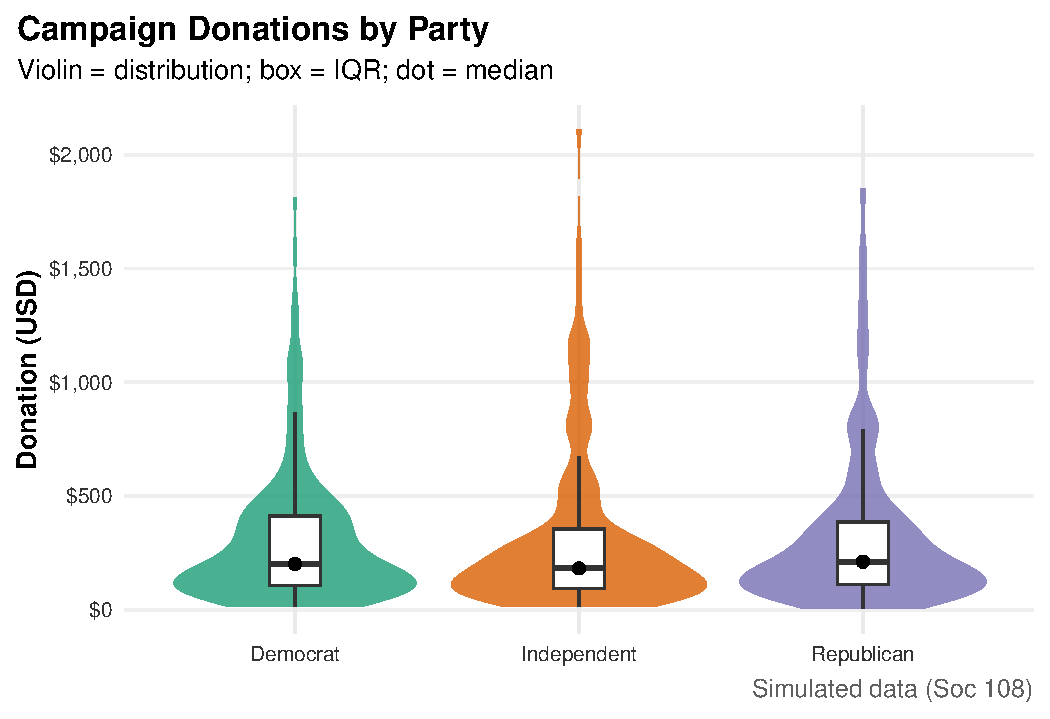
\includegraphics[keepaspectratio]{index_files/figure-pdf/ch1-donations-1.pdf}}

\section{Numeric Summaries}\label{numeric-summaries}

\begin{Shaded}
\begin{Highlighting}[]
\NormalTok{party\_share }\SpecialCharTok{|\textgreater{}} \FunctionTok{mutate}\NormalTok{(}\AttributeTok{ci95 =} \FloatTok{1.96}\SpecialCharTok{*}\FunctionTok{sqrt}\NormalTok{(pct}\SpecialCharTok{*}\NormalTok{(}\DecValTok{1}\SpecialCharTok{{-}}\NormalTok{pct)}\SpecialCharTok{/}\FunctionTok{sum}\NormalTok{(n)))}
\end{Highlighting}
\end{Shaded}

\begin{verbatim}
# A tibble: 3 x 4
  party           n   pct   ci95
  <fct>       <int> <dbl>  <dbl>
1 Democrat      225 0.375 0.0387
2 Republican    223 0.372 0.0387
3 Independent   152 0.253 0.0348
\end{verbatim}

\begin{Shaded}
\begin{Highlighting}[]
\FunctionTok{c}\NormalTok{(}\AttributeTok{turnout\_mean   =} \FunctionTok{mean}\NormalTok{(ps}\SpecialCharTok{$}\NormalTok{turnout),}
  \AttributeTok{turnout\_median =} \FunctionTok{median}\NormalTok{(ps}\SpecialCharTok{$}\NormalTok{turnout),}
  \AttributeTok{turnout\_sd     =} \FunctionTok{sd}\NormalTok{(ps}\SpecialCharTok{$}\NormalTok{turnout),}
  \AttributeTok{turnout\_iqr    =} \FunctionTok{IQR}\NormalTok{(ps}\SpecialCharTok{$}\NormalTok{turnout))}
\end{Highlighting}
\end{Shaded}

\begin{verbatim}
  turnout_mean turnout_median     turnout_sd    turnout_iqr 
      62.97833       64.00000       15.95657       23.25000 
\end{verbatim}

\begin{Shaded}
\begin{Highlighting}[]
\FunctionTok{c}\NormalTok{(}\AttributeTok{donation\_median =} \FunctionTok{median}\NormalTok{(ps}\SpecialCharTok{$}\NormalTok{donation),}
  \AttributeTok{donation\_IQR    =} \FunctionTok{IQR}\NormalTok{(ps}\SpecialCharTok{$}\NormalTok{donation),}
  \AttributeTok{donation\_p95    =} \FunctionTok{quantile}\NormalTok{(ps}\SpecialCharTok{$}\NormalTok{donation, .}\DecValTok{95}\NormalTok{))}
\end{Highlighting}
\end{Shaded}

\begin{verbatim}
 donation_median     donation_IQR donation_p95.95% 
          212.00           321.25          1207.50 
\end{verbatim}

These commands covered the essentials of data management in R: how to
inspect objects, access help, subset rows and columns, create and
transform variables, summarize and aggregate, work with strings and
vectors, and export results---all applied to the iris dataset so you can
see them in action. Mastering these basics gives you a reliable toolkit
for cleaning and organizing data in any project. In the chapters ahead,
we'll build on this foundation with more sophisticated workflows: tidy
data principles and joins across tables, reshaping (long ↔ wide),
grouped and windowed operations, regular expressions at scale, date/time
handling, functional programming with purrr, robust input/output, and
reproducible reporting and visualization pipelines.

\bookmarksetup{startatroot}

\chapter{Chapter 3: The Normal
Distribution}\label{chapter-3-the-normal-distribution}

The normal distribution is one of the most fundamental concepts in
statistics. Mastery of this topic is essential because it forms the
basis for much of the inferential work that follows. In this chapter, we
introduce the properties of the normal distribution and learn how to
calculate areas under its curve---areas that correspond to probabilities
or proportions within a given range of values.

Although it may appear somewhat out of sequence, this chapter builds
directly on our earlier discussion of how to describe and summarize
distributions. Here, we move from description to application: we use the
normal distribution to quantify the likelihood of observing values
within specified intervals. Later in the course, we will return to the
same principles when we conduct hypothesis testing, where the normal
distribution serves as a key reference model for evaluating statistical
significance.

Because of its central role in probability theory and inferential
statistics, becoming comfortable with the normal distribution is
crucial. This chapter provides the foundation and practice needed to
develop that fluency.

\begin{Shaded}
\begin{Highlighting}[]
\CommentTok{\# {-}{-}{-}{-}{-}{-}{-}{-}{-}{-}{-}{-}{-}{-}{-}{-}{-}{-}{-}{-}{-}{-}{-}{-}{-}{-}{-}{-}{-}{-}{-}{-}{-}{-}{-}{-}{-}{-}{-}{-}{-}{-}{-}{-}}
\CommentTok{\# Histogram + Normal Curve + Median Marker}
\CommentTok{\# {-}{-}{-}{-}{-}{-}{-}{-}{-}{-}{-}{-}{-}{-}{-}{-}{-}{-}{-}{-}{-}{-}{-}{-}{-}{-}{-}{-}{-}{-}{-}{-}{-}{-}{-}{-}{-}{-}{-}{-}{-}{-}{-}{-}}
 \CommentTok{\# {-}{-}{-}{-}{-}{-}{-}{-}{-}{-}{-}{-}{-}{-}{-}{-}{-}{-}{-}{-}{-}{-}{-}{-}{-}{-}{-}{-}{-}{-}{-}{-}{-}{-}{-}{-}{-}{-}{-}{-}{-}{-}{-}{-}}
\CommentTok{\# Histogram + Normal Curve + Median Marker}
\CommentTok{\# white background • light{-}blue bars • dark{-}pink line}
\CommentTok{\# {-}{-}{-}{-}{-}{-}{-}{-}{-}{-}{-}{-}{-}{-}{-}{-}{-}{-}{-}{-}{-}{-}{-}{-}{-}{-}{-}{-}{-}{-}{-}{-}{-}{-}{-}{-}{-}{-}{-}{-}{-}{-}{-}{-}}
\NormalTok{mu    }\OtherTok{\textless{}{-}} \FloatTok{69.1}
\NormalTok{sigma }\OtherTok{\textless{}{-}} \FloatTok{3.0}

\ControlFlowTok{if}\NormalTok{ (}\SpecialCharTok{!}\FunctionTok{requireNamespace}\NormalTok{(}\StringTok{"ggplot2"}\NormalTok{, }\AttributeTok{quietly =} \ConstantTok{TRUE}\NormalTok{)) }\FunctionTok{install.packages}\NormalTok{(}\StringTok{"ggplot2"}\NormalTok{)}
\FunctionTok{library}\NormalTok{(ggplot2)}

\FunctionTok{set.seed}\NormalTok{(}\DecValTok{42}\NormalTok{)}
\NormalTok{height\_in }\OtherTok{\textless{}{-}} \FunctionTok{rnorm}\NormalTok{(}\DecValTok{2000}\NormalTok{, }\AttributeTok{mean =}\NormalTok{ mu, }\AttributeTok{sd =}\NormalTok{ sigma)}

\NormalTok{df }\OtherTok{\textless{}{-}} \FunctionTok{data.frame}\NormalTok{(}\AttributeTok{height\_in =}\NormalTok{ height\_in)}
\NormalTok{med\_val }\OtherTok{\textless{}{-}} \FunctionTok{median}\NormalTok{(df}\SpecialCharTok{$}\NormalTok{height\_in)}

\CommentTok{\# {-}{-}{-} colors {-}{-}{-}}
\NormalTok{fill\_ltblue   }\OtherTok{\textless{}{-}} \StringTok{"\#A7D8FF"}  \CommentTok{\# bar fill (light blue)}
\NormalTok{border\_blue   }\OtherTok{\textless{}{-}} \StringTok{"\#2C7FB8"}  \CommentTok{\# bar border}
\NormalTok{curve\_blue    }\OtherTok{\textless{}{-}} \StringTok{"\#C2185B"}  \CommentTok{\# normal curve}
\NormalTok{median\_pink   }\OtherTok{\textless{}{-}} \StringTok{"black"}  \CommentTok{\# dark pink median line \& label}

\NormalTok{p }\OtherTok{\textless{}{-}} \FunctionTok{ggplot}\NormalTok{(df, }\FunctionTok{aes}\NormalTok{(}\AttributeTok{x =}\NormalTok{ height\_in)) }\SpecialCharTok{+}
  \CommentTok{\# Histogram on density scale so curve aligns}
  \FunctionTok{geom\_histogram}\NormalTok{(}\FunctionTok{aes}\NormalTok{(}\AttributeTok{y =} \FunctionTok{after\_stat}\NormalTok{(density)),}
                 \AttributeTok{binwidth =} \FloatTok{0.4}\NormalTok{,}
                 \AttributeTok{fill =}\NormalTok{ fill\_ltblue,}
                 \AttributeTok{color =}\NormalTok{ border\_blue,}
                 \AttributeTok{linewidth =} \FloatTok{0.5}\NormalTok{,}
                 \AttributeTok{alpha =} \FloatTok{0.9}\NormalTok{) }\SpecialCharTok{+}
  \CommentTok{\# Normal curve with specified mu/sigma}
  \FunctionTok{stat\_function}\NormalTok{(}\AttributeTok{fun =}\NormalTok{ dnorm,}
                \AttributeTok{args =} \FunctionTok{list}\NormalTok{(}\AttributeTok{mean =}\NormalTok{ mu, }\AttributeTok{sd =}\NormalTok{ sigma),}
                \AttributeTok{linewidth =} \FloatTok{1.2}\NormalTok{,}
                \AttributeTok{color =}\NormalTok{ curve\_blue) }\SpecialCharTok{+}
  \CommentTok{\# Median marker (dark pink)}
  \FunctionTok{geom\_vline}\NormalTok{(}\AttributeTok{xintercept =}\NormalTok{ med\_val,}
             \AttributeTok{linewidth =} \DecValTok{1}\NormalTok{,}
             \AttributeTok{linetype =} \StringTok{"longdash"}\NormalTok{,}
             \AttributeTok{color =}\NormalTok{ median\_pink) }\SpecialCharTok{+}
  \FunctionTok{annotate}\NormalTok{(}\StringTok{"text"}\NormalTok{,}
           \AttributeTok{x =}\NormalTok{ med\_val,}
           \AttributeTok{y =} \FunctionTok{max}\NormalTok{(}\FunctionTok{dnorm}\NormalTok{(}\FunctionTok{seq}\NormalTok{(mu }\SpecialCharTok{{-}} \DecValTok{4}\SpecialCharTok{*}\NormalTok{sigma, mu }\SpecialCharTok{+} \DecValTok{4}\SpecialCharTok{*}\NormalTok{sigma, }\AttributeTok{length.out =} \DecValTok{2000}\NormalTok{), mu, sigma)) }\SpecialCharTok{*} \FloatTok{0.92}\NormalTok{,}
           \AttributeTok{label =} \FunctionTok{sprintf}\NormalTok{(}\StringTok{"Median = \%.2f in"}\NormalTok{, med\_val),}
           \AttributeTok{vjust =} \SpecialCharTok{{-}}\FloatTok{0.3}\NormalTok{,}
           \AttributeTok{color =}\NormalTok{ median\_pink,}
           \AttributeTok{fontface =} \StringTok{"bold"}\NormalTok{) }\SpecialCharTok{+}
  \CommentTok{\# Clean white background}
  \FunctionTok{theme\_minimal}\NormalTok{(}\AttributeTok{base\_size =} \DecValTok{13}\NormalTok{) }\SpecialCharTok{+}
  \FunctionTok{theme}\NormalTok{(}
    \AttributeTok{panel.background   =} \FunctionTok{element\_rect}\NormalTok{(}\AttributeTok{fill =} \StringTok{"white"}\NormalTok{, }\AttributeTok{color =} \ConstantTok{NA}\NormalTok{),}
    \AttributeTok{plot.background    =} \FunctionTok{element\_rect}\NormalTok{(}\AttributeTok{fill =} \StringTok{"white"}\NormalTok{, }\AttributeTok{color =} \ConstantTok{NA}\NormalTok{),}
    \AttributeTok{panel.grid.minor   =} \FunctionTok{element\_blank}\NormalTok{(),}
    \AttributeTok{panel.grid.major.x =} \FunctionTok{element\_blank}\NormalTok{(),}
    \AttributeTok{panel.grid.major.y =} \FunctionTok{element\_line}\NormalTok{(}\AttributeTok{color =} \StringTok{"\#EEEEEE"}\NormalTok{)}
\NormalTok{  ) }\SpecialCharTok{+}
  \FunctionTok{labs}\NormalTok{(}\AttributeTok{x =} \StringTok{"Height (inches)"}\NormalTok{, }\AttributeTok{y =} \StringTok{"Density"}\NormalTok{) }\SpecialCharTok{+}
  \FunctionTok{coord\_cartesian}\NormalTok{(}\AttributeTok{xlim =} \FunctionTok{c}\NormalTok{(mu }\SpecialCharTok{{-}} \DecValTok{4}\SpecialCharTok{*}\NormalTok{sigma, mu }\SpecialCharTok{+} \DecValTok{4}\SpecialCharTok{*}\NormalTok{sigma))}

\NormalTok{p}
\end{Highlighting}
\end{Shaded}

\pandocbounded{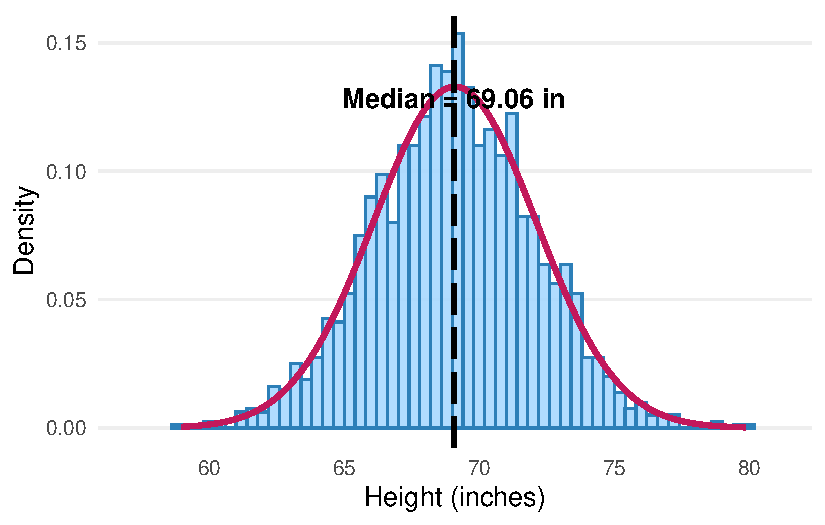
\includegraphics[keepaspectratio]{index_files/figure-pdf/unnamed-chunk-23-1.pdf}}

This histogram depicts the distribution of adult men's heights in the
United States based on national data. According to the Centers for
Disease Control and Prevention (CDC), the average height for adult men
in the U.S. is approximately 69.1 inches (about 5 feet 9 inches). The
distribution is roughly symmetric, so both the mean and median fall
close to this value. The tallest men in the population reach about 78
inches (6 feet 6 inches), while the shortest are around 62 inches (5
feet 2 inches).

Each bar in the histogram represents the proportion of men whose heights
fall within a particular range. Although the histogram displays these
proportions in discrete intervals, we can visualize the data more
smoothly by imagining a continuous curve---typically a normal
distribution---drawn over the bars. This curve provides a concise
summary of how men's heights are distributed nationwide, showing that
most men cluster near the average, with fewer at the extremes of very
short or very tall.

When working with real data, a histogram provides a discrete
approximation of a distribution. In the density curve below, each bar
represents the proportion of cases falling within a specific range. For
example, the histogram below shows the distribution of adult men's
heights in the United States. Suppose we are interested in the
proportion of men whose height is less than or equal to 69 inches. By
summing the relative frequencies of the bars up to this value, we find
that approximately 0.30, or 30\%, of men are 69 inches tall or shorter.
We can also represent the same distribution as a smooth density curve,
which provides a continuous approximation of the underlying probability
distribution---in this case, the normal distribution. The area under the
density curve to the left of 69 inches represents the same probability,
and when computed analytically using the properties of the normal
distribution, we obtain an area of approximately 0.29. Although the
results from the histogram and the smooth curve are not exactly
identical, the difference is quite small. The density curve serves as an
excellent model for the distribution, allowing us to calculate
probabilities (areas) precisely and efficiently.

\begin{Shaded}
\begin{Highlighting}[]
\FunctionTok{library}\NormalTok{(ggplot2)}
\FunctionTok{library}\NormalTok{(gridExtra)}
\FunctionTok{library}\NormalTok{(grid)}

\NormalTok{fill\_green }\OtherTok{\textless{}{-}} \StringTok{"\#7FC97F"}
\NormalTok{fill\_yellow }\OtherTok{\textless{}{-}} \StringTok{"\#FFF59D"}
\NormalTok{curve\_blue }\OtherTok{\textless{}{-}} \StringTok{"\#2C7FB8"}
\NormalTok{panel\_blue }\OtherTok{\textless{}{-}} \StringTok{"\#DDEEFF"}
\NormalTok{grid\_major\_red }\OtherTok{\textless{}{-}} \StringTok{"\#F6C5C5"}
\NormalTok{grid\_minor\_red }\OtherTok{\textless{}{-}} \StringTok{"\#FBE6E6"}
\NormalTok{accent\_dark  }\OtherTok{\textless{}{-}} \StringTok{"\#1F4E79"}
\NormalTok{mean\_color   }\OtherTok{\textless{}{-}} \StringTok{"\#FF5733"}

\NormalTok{the\_theme\_big }\OtherTok{\textless{}{-}} \FunctionTok{theme\_minimal}\NormalTok{(}\AttributeTok{base\_size =} \DecValTok{16}\NormalTok{) }\SpecialCharTok{+}
  \FunctionTok{theme}\NormalTok{(}
    \AttributeTok{panel.background =} \FunctionTok{element\_rect}\NormalTok{(}\AttributeTok{fill =}\NormalTok{ panel\_blue, }\AttributeTok{color =} \ConstantTok{NA}\NormalTok{),}
    \AttributeTok{plot.background  =} \FunctionTok{element\_rect}\NormalTok{(}\AttributeTok{fill =} \StringTok{"white"}\NormalTok{, }\AttributeTok{color =} \ConstantTok{NA}\NormalTok{),}
    \AttributeTok{panel.grid.major =} \FunctionTok{element\_line}\NormalTok{(}\AttributeTok{color =}\NormalTok{ grid\_major\_red, }\AttributeTok{linewidth =} \FloatTok{0.5}\NormalTok{),}
    \AttributeTok{panel.grid.minor =} \FunctionTok{element\_line}\NormalTok{(}\AttributeTok{color =}\NormalTok{ grid\_minor\_red, }\AttributeTok{linewidth =} \FloatTok{0.3}\NormalTok{),}
    \AttributeTok{panel.grid.major.x =} \FunctionTok{element\_line}\NormalTok{(}\AttributeTok{color =}\NormalTok{ grid\_major\_red),}
    \AttributeTok{legend.position =} \StringTok{"none"}\NormalTok{,}
    \AttributeTok{plot.title =} \FunctionTok{element\_text}\NormalTok{(}\AttributeTok{face =} \StringTok{"bold"}\NormalTok{, }\AttributeTok{size =} \DecValTok{18}\NormalTok{)}
\NormalTok{  )}

\NormalTok{mu }\OtherTok{\textless{}{-}} \DecValTok{0}
\NormalTok{sigma\_left  }\OtherTok{\textless{}{-}} \FloatTok{1.4}
\NormalTok{sigma\_right }\OtherTok{\textless{}{-}} \FloatTok{0.6}

\NormalTok{xL }\OtherTok{\textless{}{-}} \FunctionTok{seq}\NormalTok{(mu }\SpecialCharTok{{-}} \DecValTok{4}\SpecialCharTok{*}\NormalTok{sigma\_left, mu }\SpecialCharTok{+} \DecValTok{4}\SpecialCharTok{*}\NormalTok{sigma\_left, }\AttributeTok{length.out =} \DecValTok{1200}\NormalTok{)}
\NormalTok{yL }\OtherTok{\textless{}{-}} \FunctionTok{dnorm}\NormalTok{(xL, mu, sigma\_left)}
\NormalTok{dfL }\OtherTok{\textless{}{-}} \FunctionTok{data.frame}\NormalTok{(}\AttributeTok{x =}\NormalTok{ xL, }\AttributeTok{y =}\NormalTok{ yL)}
\NormalTok{shadeL }\OtherTok{\textless{}{-}} \FunctionTok{subset}\NormalTok{(dfL, x }\SpecialCharTok{\textgreater{}=}\NormalTok{ mu }\SpecialCharTok{{-}}\NormalTok{ sigma\_left }\SpecialCharTok{\&}\NormalTok{ x }\SpecialCharTok{\textless{}=}\NormalTok{ mu }\SpecialCharTok{+}\NormalTok{ sigma\_left)}

\NormalTok{xR }\OtherTok{\textless{}{-}} \FunctionTok{seq}\NormalTok{(mu }\SpecialCharTok{{-}} \DecValTok{4}\SpecialCharTok{*}\NormalTok{sigma\_left, mu }\SpecialCharTok{+} \DecValTok{4}\SpecialCharTok{*}\NormalTok{sigma\_left, }\AttributeTok{length.out =} \DecValTok{1200}\NormalTok{)}
\NormalTok{yR }\OtherTok{\textless{}{-}} \FunctionTok{dnorm}\NormalTok{(xR, mu, sigma\_right)}
\NormalTok{dfR }\OtherTok{\textless{}{-}} \FunctionTok{data.frame}\NormalTok{(}\AttributeTok{x =}\NormalTok{ xR, }\AttributeTok{y =}\NormalTok{ yR)}
\NormalTok{shadeR }\OtherTok{\textless{}{-}} \FunctionTok{subset}\NormalTok{(dfR, x }\SpecialCharTok{\textgreater{}=}\NormalTok{ mu }\SpecialCharTok{{-}}\NormalTok{ sigma\_right }\SpecialCharTok{\&}\NormalTok{ x }\SpecialCharTok{\textless{}=}\NormalTok{ mu }\SpecialCharTok{+}\NormalTok{ sigma\_right)}

\NormalTok{ymax }\OtherTok{\textless{}{-}} \FunctionTok{max}\NormalTok{(}\FunctionTok{c}\NormalTok{(yL, yR)) }\SpecialCharTok{*} \FloatTok{1.10}

\NormalTok{p\_left }\OtherTok{\textless{}{-}} \FunctionTok{ggplot}\NormalTok{(dfL, }\FunctionTok{aes}\NormalTok{(x, y)) }\SpecialCharTok{+}
  \FunctionTok{geom\_area}\NormalTok{(}\AttributeTok{fill =}\NormalTok{ fill\_green, }\AttributeTok{alpha =} \FloatTok{0.60}\NormalTok{) }\SpecialCharTok{+}
  \FunctionTok{geom\_area}\NormalTok{(}\AttributeTok{data =}\NormalTok{ shadeL, }\FunctionTok{aes}\NormalTok{(x, y), }\AttributeTok{fill =}\NormalTok{ fill\_yellow, }\AttributeTok{alpha =} \FloatTok{0.95}\NormalTok{) }\SpecialCharTok{+}
  \FunctionTok{geom\_line}\NormalTok{(}\AttributeTok{color =}\NormalTok{ curve\_blue, }\AttributeTok{linewidth =} \FloatTok{1.4}\NormalTok{) }\SpecialCharTok{+}
  \FunctionTok{geom\_vline}\NormalTok{(}\AttributeTok{xintercept =}\NormalTok{ mu, }\AttributeTok{color =}\NormalTok{ mean\_color, }\AttributeTok{linewidth =} \FloatTok{1.4}\NormalTok{) }\SpecialCharTok{+}
  \FunctionTok{annotate}\NormalTok{(}\StringTok{"text"}\NormalTok{, }\AttributeTok{x =}\NormalTok{ mu, }\AttributeTok{y =}\NormalTok{ ymax}\SpecialCharTok{*}\FloatTok{0.07}\NormalTok{, }\AttributeTok{label =} \StringTok{"\textbackslash{}u03BC"}\NormalTok{, }\AttributeTok{color =}\NormalTok{ mean\_color, }\AttributeTok{fontface =} \StringTok{"bold"}\NormalTok{) }\SpecialCharTok{+}
  \FunctionTok{annotate}\NormalTok{(}\StringTok{"text"}\NormalTok{, }\AttributeTok{x =}\NormalTok{ mu }\SpecialCharTok{{-}}\NormalTok{ sigma\_left}\SpecialCharTok{*}\FloatTok{1.9}\NormalTok{, }\AttributeTok{y =}\NormalTok{ ymax}\SpecialCharTok{*}\FloatTok{0.92}\NormalTok{, }\AttributeTok{label =} \StringTok{"\textbackslash{}u03C3 larger (wider spread)"}\NormalTok{, }\AttributeTok{color =}\NormalTok{ accent\_dark, }\AttributeTok{fontface =} \StringTok{"bold"}\NormalTok{, }\AttributeTok{hjust =} \DecValTok{0}\NormalTok{) }\SpecialCharTok{+}
  \FunctionTok{geom\_segment}\NormalTok{(}\FunctionTok{aes}\NormalTok{(}\AttributeTok{x =}\NormalTok{ mu }\SpecialCharTok{{-}}\NormalTok{ sigma\_left}\SpecialCharTok{*}\FloatTok{0.7}\NormalTok{, }\AttributeTok{y =}\NormalTok{ ymax}\SpecialCharTok{*}\FloatTok{0.90}\NormalTok{, }\AttributeTok{xend =}\NormalTok{ mu }\SpecialCharTok{{-}}\NormalTok{ sigma\_left, }\AttributeTok{yend =} \FunctionTok{dnorm}\NormalTok{(mu }\SpecialCharTok{{-}}\NormalTok{ sigma\_left, mu, sigma\_left)}\SpecialCharTok{*}\FloatTok{0.95}\NormalTok{),}
               \AttributeTok{arrow =} \FunctionTok{arrow}\NormalTok{(}\AttributeTok{length =} \FunctionTok{unit}\NormalTok{(}\FloatTok{0.12}\NormalTok{, }\StringTok{"inches"}\NormalTok{)), }\AttributeTok{color =}\NormalTok{ accent\_dark) }\SpecialCharTok{+}
  \FunctionTok{labs}\NormalTok{(}\AttributeTok{title =} \StringTok{"Normal distribution with larger \textbackslash{}u03C3"}\NormalTok{, }\AttributeTok{x =} \StringTok{"Value"}\NormalTok{, }\AttributeTok{y =} \StringTok{"Density"}\NormalTok{) }\SpecialCharTok{+}
  \FunctionTok{coord\_cartesian}\NormalTok{(}\AttributeTok{ylim =} \FunctionTok{c}\NormalTok{(}\DecValTok{0}\NormalTok{, ymax)) }\SpecialCharTok{+}
\NormalTok{  the\_theme\_big}

\NormalTok{p\_right }\OtherTok{\textless{}{-}} \FunctionTok{ggplot}\NormalTok{(dfR, }\FunctionTok{aes}\NormalTok{(x, y)) }\SpecialCharTok{+}
  \FunctionTok{geom\_area}\NormalTok{(}\AttributeTok{fill =}\NormalTok{ fill\_green, }\AttributeTok{alpha =} \FloatTok{0.60}\NormalTok{) }\SpecialCharTok{+}
  \FunctionTok{geom\_area}\NormalTok{(}\AttributeTok{data =}\NormalTok{ shadeR, }\FunctionTok{aes}\NormalTok{(x, y), }\AttributeTok{fill =}\NormalTok{ fill\_yellow, }\AttributeTok{alpha =} \FloatTok{0.95}\NormalTok{) }\SpecialCharTok{+}
  \FunctionTok{geom\_line}\NormalTok{(}\AttributeTok{color =}\NormalTok{ curve\_blue, }\AttributeTok{linewidth =} \FloatTok{1.4}\NormalTok{) }\SpecialCharTok{+}
  \FunctionTok{geom\_vline}\NormalTok{(}\AttributeTok{xintercept =}\NormalTok{ mu, }\AttributeTok{color =}\NormalTok{ mean\_color, }\AttributeTok{linewidth =} \FloatTok{1.4}\NormalTok{) }\SpecialCharTok{+}
  \FunctionTok{annotate}\NormalTok{(}\StringTok{"text"}\NormalTok{, }\AttributeTok{x =}\NormalTok{ mu, }\AttributeTok{y =}\NormalTok{ ymax}\SpecialCharTok{*}\FloatTok{0.07}\NormalTok{, }\AttributeTok{label =} \StringTok{"\textbackslash{}u03BC"}\NormalTok{, }\AttributeTok{color =}\NormalTok{ mean\_color, }\AttributeTok{fontface =} \StringTok{"bold"}\NormalTok{) }\SpecialCharTok{+}
  \FunctionTok{annotate}\NormalTok{(}\StringTok{"text"}\NormalTok{, }\AttributeTok{x =}\NormalTok{ mu }\SpecialCharTok{+}\NormalTok{ sigma\_left}\SpecialCharTok{*}\FloatTok{0.9}\NormalTok{, }\AttributeTok{y =}\NormalTok{ ymax}\SpecialCharTok{*}\FloatTok{0.92}\NormalTok{, }\AttributeTok{label =} \StringTok{"\textbackslash{}u03C3 smaller (narrower spread)"}\NormalTok{, }\AttributeTok{color =}\NormalTok{ accent\_dark, }\AttributeTok{fontface =} \StringTok{"bold"}\NormalTok{, }\AttributeTok{hjust =} \DecValTok{0}\NormalTok{) }\SpecialCharTok{+}
  \FunctionTok{geom\_segment}\NormalTok{(}\FunctionTok{aes}\NormalTok{(}\AttributeTok{x =}\NormalTok{ mu }\SpecialCharTok{+}\NormalTok{ sigma\_right}\SpecialCharTok{*}\FloatTok{0.7}\NormalTok{, }\AttributeTok{y =}\NormalTok{ ymax}\SpecialCharTok{*}\FloatTok{0.90}\NormalTok{, }\AttributeTok{xend =}\NormalTok{ mu }\SpecialCharTok{+}\NormalTok{ sigma\_right, }\AttributeTok{yend =} \FunctionTok{dnorm}\NormalTok{(mu }\SpecialCharTok{+}\NormalTok{ sigma\_right, mu, sigma\_right)}\SpecialCharTok{*}\FloatTok{0.95}\NormalTok{),}
               \AttributeTok{arrow =} \FunctionTok{arrow}\NormalTok{(}\AttributeTok{length =} \FunctionTok{unit}\NormalTok{(}\FloatTok{0.12}\NormalTok{, }\StringTok{"inches"}\NormalTok{)), }\AttributeTok{color =}\NormalTok{ accent\_dark) }\SpecialCharTok{+}
  \FunctionTok{labs}\NormalTok{(}\AttributeTok{title =} \StringTok{"Normal distribution with smaller \textbackslash{}u03C3"}\NormalTok{, }\AttributeTok{x =} \StringTok{"Value"}\NormalTok{, }\AttributeTok{y =} \StringTok{"Density"}\NormalTok{) }\SpecialCharTok{+}
  \FunctionTok{coord\_cartesian}\NormalTok{(}\AttributeTok{ylim =} \FunctionTok{c}\NormalTok{(}\DecValTok{0}\NormalTok{, ymax)) }\SpecialCharTok{+}
\NormalTok{  the\_theme\_big}

\FunctionTok{grid.arrange}\NormalTok{(p\_left, p\_right, }\AttributeTok{ncol =} \DecValTok{2}\NormalTok{,}
             \AttributeTok{top =} \StringTok{"The Normal Distribution: Same \textbackslash{}u03BC, Different \textbackslash{}u03C3"}\NormalTok{)}
\end{Highlighting}
\end{Shaded}

\pandocbounded{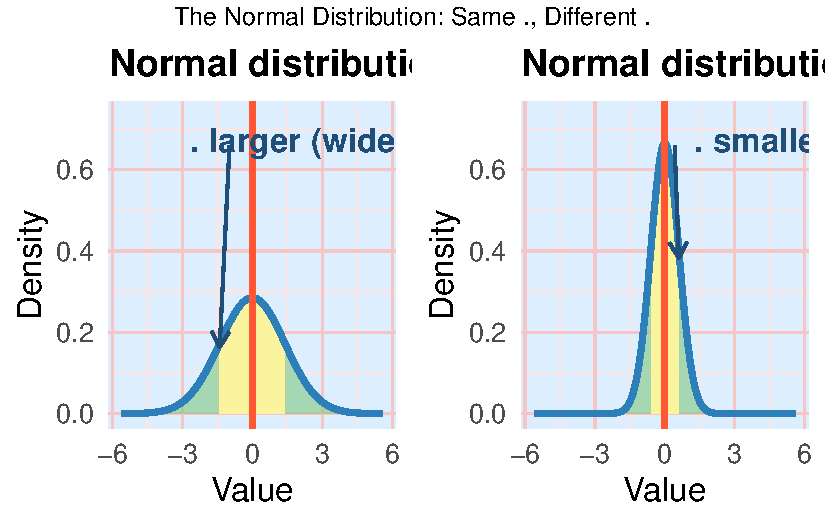
\includegraphics[keepaspectratio]{index_files/figure-pdf/unnamed-chunk-24-1.pdf}}

A density curve is a smooth, mathematical model that represents the
overall pattern of a distribution. Rather than depicting frequencies
through discrete bars---as a histogram does---a density curve provides a
continuous approximation that shows the relative proportion of
observations within any range of values.

For instance, consider the distribution of adult men's heights in the
United States. The density curve drawn around this distribution
describes how the probability of observing a particular height varies
across the population. The area under the curve between two points
corresponds to the proportion of individuals whose heights fall within
that range. By definition, the total area under the density curve is
equal to 1, meaning that it represents 100\% of all observations in the
distribution. Thus, just as every observation in a dataset contributes
to the total area of a histogram, every observation in a population
contributes to the total area under its density curve.

In short, the density curve serves as a smooth, idealized version of the
histogram---one that captures the same essential information about
relative frequencies and proportions, but in a continuous form suitable
for precise probability calculations.

Density curves share many of the same descriptive properties as the
frequency distributions we have studied through histograms and
stemplots. Like those, they possess a center, a shape, and a spread.
These curves provide an idealized mathematical model of a distribution,
enabling us to describe its overall pattern in a continuous way.

Just as we did with histograms, we can identify measures of central
tendency---specifically, the mean and the median---for a density curve.
The median divides the total area under the curve into two equal halves,
such that 50\% of observations lie below it and 50\% lie above it. The
mean, by contrast, is the point at which the curve would balance if it
were made of a uniform sheet of material.

In a perfectly symmetric distribution, the mean and median coincide. For
example, the distribution of adult men's heights in the United States is
approximately symmetric, and therefore the mean (around 69 inches) is
nearly equal to the median. In such cases, half of the population lies
below this central value and half lies above it.

However, when a distribution is skewed, the relationship between the
mean and median changes. In a right-skewed distribution---such as the
distribution of household income---the long tail of higher values pulls
the mean to the right of the median. Conversely, in a left-skewed
distribution, the mean lies to the left of the median. The greater the
skewness, the larger this separation becomes.

Regardless of the distribution's shape, the area under the curve always
represents the total proportion of observations, which by definition
equals 1 (or 100\%). Dividing the curve at the median ensures that half
of this total area lies on each side.

\begin{Shaded}
\begin{Highlighting}[]
\FunctionTok{library}\NormalTok{(ggplot2)}
\FunctionTok{library}\NormalTok{(ggplot2)}

\CommentTok{\# Parameters for normal distribution}
\NormalTok{mu }\OtherTok{\textless{}{-}} \DecValTok{0}
\NormalTok{sigma }\OtherTok{\textless{}{-}} \DecValTok{1}

\CommentTok{\# Create data for the curves}
\NormalTok{x\_vals }\OtherTok{\textless{}{-}} \FunctionTok{seq}\NormalTok{(mu }\SpecialCharTok{{-}} \DecValTok{4}\SpecialCharTok{*}\NormalTok{sigma, mu }\SpecialCharTok{+} \DecValTok{4}\SpecialCharTok{*}\NormalTok{sigma, }\AttributeTok{length.out =} \DecValTok{1000}\NormalTok{)}
\NormalTok{y\_vals }\OtherTok{\textless{}{-}} \FunctionTok{dnorm}\NormalTok{(x\_vals, }\AttributeTok{mean =}\NormalTok{ mu, }\AttributeTok{sd =}\NormalTok{ sigma)}

\CommentTok{\# Create main dataframe}
\NormalTok{df }\OtherTok{\textless{}{-}} \FunctionTok{data.frame}\NormalTok{(}\AttributeTok{x =}\NormalTok{ x\_vals, }\AttributeTok{y =}\NormalTok{ y\_vals)}

\CommentTok{\# Inflection points occur at mu ± sigma}
\NormalTok{inflection\_left }\OtherTok{\textless{}{-}}\NormalTok{ mu }\SpecialCharTok{{-}}\NormalTok{ sigma}
\NormalTok{inflection\_right }\OtherTok{\textless{}{-}}\NormalTok{ mu }\SpecialCharTok{+}\NormalTok{ sigma}
\NormalTok{inflection\_y }\OtherTok{\textless{}{-}} \FunctionTok{dnorm}\NormalTok{(inflection\_left, }\AttributeTok{mean =}\NormalTok{ mu, }\AttributeTok{sd =}\NormalTok{ sigma)}

\CommentTok{\# Create plot}
\FunctionTok{ggplot}\NormalTok{(df, }\FunctionTok{aes}\NormalTok{(}\AttributeTok{x =}\NormalTok{ x, }\AttributeTok{y =}\NormalTok{ y)) }\SpecialCharTok{+}
  \CommentTok{\# Fill under curve}
  \FunctionTok{geom\_area}\NormalTok{(}\AttributeTok{fill =} \StringTok{"lightblue"}\NormalTok{, }\AttributeTok{alpha =} \FloatTok{0.5}\NormalTok{) }\SpecialCharTok{+}
  \CommentTok{\# Main curve}
  \FunctionTok{geom\_line}\NormalTok{(}\AttributeTok{color =} \StringTok{"darkblue"}\NormalTok{, }\AttributeTok{linewidth =} \FloatTok{1.2}\NormalTok{) }\SpecialCharTok{+}
  
  \CommentTok{\# Vertical line at mean (mu)}
  \FunctionTok{geom\_vline}\NormalTok{(}\AttributeTok{xintercept =}\NormalTok{ mu, }\AttributeTok{color =} \StringTok{"black"}\NormalTok{, }\AttributeTok{linewidth =} \FloatTok{0.8}\NormalTok{) }\SpecialCharTok{+}
  
  \CommentTok{\# Vertical lines at inflection points}
  \FunctionTok{geom\_segment}\NormalTok{(}\FunctionTok{aes}\NormalTok{(}\AttributeTok{x =}\NormalTok{ inflection\_left, }\AttributeTok{xend =}\NormalTok{ inflection\_left,}
                   \AttributeTok{y =} \DecValTok{0}\NormalTok{, }\AttributeTok{yend =}\NormalTok{ inflection\_y),}
               \AttributeTok{color =} \StringTok{"red"}\NormalTok{, }\AttributeTok{linewidth =} \FloatTok{0.8}\NormalTok{, }\AttributeTok{linetype =} \StringTok{"dashed"}\NormalTok{) }\SpecialCharTok{+}
  \FunctionTok{geom\_segment}\NormalTok{(}\FunctionTok{aes}\NormalTok{(}\AttributeTok{x =}\NormalTok{ inflection\_right, }\AttributeTok{xend =}\NormalTok{ inflection\_right,}
                   \AttributeTok{y =} \DecValTok{0}\NormalTok{, }\AttributeTok{yend =}\NormalTok{ inflection\_y),}
               \AttributeTok{color =} \StringTok{"red"}\NormalTok{, }\AttributeTok{linewidth =} \FloatTok{0.8}\NormalTok{, }\AttributeTok{linetype =} \StringTok{"dashed"}\NormalTok{) }\SpecialCharTok{+}
  
  \CommentTok{\# Horizontal lines showing sigma distance}
  \FunctionTok{geom\_segment}\NormalTok{(}\FunctionTok{aes}\NormalTok{(}\AttributeTok{x =}\NormalTok{ mu, }\AttributeTok{xend =}\NormalTok{ inflection\_left,}
                   \AttributeTok{y =}\NormalTok{ inflection\_y }\SpecialCharTok{*} \FloatTok{0.5}\NormalTok{, }\AttributeTok{yend =}\NormalTok{ inflection\_y }\SpecialCharTok{*} \FloatTok{0.5}\NormalTok{),}
               \AttributeTok{color =} \StringTok{"black"}\NormalTok{, }\AttributeTok{linewidth =} \FloatTok{0.6}\NormalTok{,}
               \AttributeTok{arrow =} \FunctionTok{arrow}\NormalTok{(}\AttributeTok{ends =} \StringTok{"both"}\NormalTok{, }\AttributeTok{length =} \FunctionTok{unit}\NormalTok{(}\FloatTok{0.15}\NormalTok{, }\StringTok{"cm"}\NormalTok{))) }\SpecialCharTok{+}
  \FunctionTok{geom\_segment}\NormalTok{(}\FunctionTok{aes}\NormalTok{(}\AttributeTok{x =}\NormalTok{ mu, }\AttributeTok{xend =}\NormalTok{ inflection\_right,}
                   \AttributeTok{y =}\NormalTok{ inflection\_y }\SpecialCharTok{*} \FloatTok{0.5}\NormalTok{, }\AttributeTok{yend =}\NormalTok{ inflection\_y }\SpecialCharTok{*} \FloatTok{0.5}\NormalTok{),}
               \AttributeTok{color =} \StringTok{"black"}\NormalTok{, }\AttributeTok{linewidth =} \FloatTok{0.6}\NormalTok{,}
               \AttributeTok{arrow =} \FunctionTok{arrow}\NormalTok{(}\AttributeTok{ends =} \StringTok{"both"}\NormalTok{, }\AttributeTok{length =} \FunctionTok{unit}\NormalTok{(}\FloatTok{0.15}\NormalTok{, }\StringTok{"cm"}\NormalTok{))) }\SpecialCharTok{+}
  
  \CommentTok{\# Labels}
  \FunctionTok{annotate}\NormalTok{(}\StringTok{"text"}\NormalTok{, }\AttributeTok{x =}\NormalTok{ mu, }\AttributeTok{y =} \SpecialCharTok{{-}}\FloatTok{0.02}\NormalTok{, }\AttributeTok{label =} \StringTok{"μ"}\NormalTok{, }\AttributeTok{size =} \DecValTok{6}\NormalTok{, }\AttributeTok{fontface =} \StringTok{"bold"}\NormalTok{) }\SpecialCharTok{+}
  \FunctionTok{annotate}\NormalTok{(}\StringTok{"text"}\NormalTok{, }\AttributeTok{x =}\NormalTok{ (mu }\SpecialCharTok{+}\NormalTok{ inflection\_left)}\SpecialCharTok{/}\DecValTok{2}\NormalTok{, }\AttributeTok{y =}\NormalTok{ inflection\_y }\SpecialCharTok{*} \FloatTok{0.55}\NormalTok{,}
           \AttributeTok{label =} \StringTok{"σ"}\NormalTok{, }\AttributeTok{size =} \DecValTok{5}\NormalTok{, }\AttributeTok{fontface =} \StringTok{"italic"}\NormalTok{) }\SpecialCharTok{+}
  \FunctionTok{annotate}\NormalTok{(}\StringTok{"text"}\NormalTok{, }\AttributeTok{x =}\NormalTok{ (mu }\SpecialCharTok{+}\NormalTok{ inflection\_right)}\SpecialCharTok{/}\DecValTok{2}\NormalTok{, }\AttributeTok{y =}\NormalTok{ inflection\_y }\SpecialCharTok{*} \FloatTok{0.55}\NormalTok{,}
           \AttributeTok{label =} \StringTok{"σ"}\NormalTok{, }\AttributeTok{size =} \DecValTok{5}\NormalTok{, }\AttributeTok{fontface =} \StringTok{"italic"}\NormalTok{) }\SpecialCharTok{+}
  
  \CommentTok{\# Inflection point labels}
  \FunctionTok{annotate}\NormalTok{(}\StringTok{"text"}\NormalTok{, }\AttributeTok{x =}\NormalTok{ inflection\_left }\SpecialCharTok{{-}} \FloatTok{0.3}\NormalTok{, }\AttributeTok{y =}\NormalTok{ inflection\_y }\SpecialCharTok{+} \FloatTok{0.03}\NormalTok{,}
           \AttributeTok{label =} \StringTok{"inflection}\SpecialCharTok{\textbackslash{}n}\StringTok{point"}\NormalTok{, }\AttributeTok{size =} \FloatTok{3.5}\NormalTok{, }\AttributeTok{hjust =} \DecValTok{1}\NormalTok{) }\SpecialCharTok{+}
  \FunctionTok{annotate}\NormalTok{(}\StringTok{"text"}\NormalTok{, }\AttributeTok{x =}\NormalTok{ inflection\_right }\SpecialCharTok{+} \FloatTok{0.3}\NormalTok{, }\AttributeTok{y =}\NormalTok{ inflection\_y }\SpecialCharTok{+} \FloatTok{0.03}\NormalTok{,}
           \AttributeTok{label =} \StringTok{"inflection}\SpecialCharTok{\textbackslash{}n}\StringTok{point"}\NormalTok{, }\AttributeTok{size =} \FloatTok{3.5}\NormalTok{, }\AttributeTok{hjust =} \DecValTok{0}\NormalTok{) }\SpecialCharTok{+}
  
  \CommentTok{\# Concavity labels}
  \FunctionTok{annotate}\NormalTok{(}\StringTok{"text"}\NormalTok{, }\AttributeTok{x =}\NormalTok{ inflection\_left }\SpecialCharTok{{-}} \DecValTok{1}\NormalTok{, }\AttributeTok{y =} \FunctionTok{dnorm}\NormalTok{(inflection\_left }\SpecialCharTok{{-}} \DecValTok{1}\NormalTok{, mu, sigma) }\SpecialCharTok{+} \FloatTok{0.05}\NormalTok{,}
           \AttributeTok{label =} \StringTok{"concave}\SpecialCharTok{\textbackslash{}n}\StringTok{down"}\NormalTok{, }\AttributeTok{size =} \FloatTok{3.5}\NormalTok{) }\SpecialCharTok{+}
  \FunctionTok{annotate}\NormalTok{(}\StringTok{"text"}\NormalTok{, }\AttributeTok{x =} \DecValTok{0}\NormalTok{, }\AttributeTok{y =} \FunctionTok{dnorm}\NormalTok{(}\DecValTok{0}\NormalTok{, mu, sigma) }\SpecialCharTok{+} \FloatTok{0.05}\NormalTok{,}
           \AttributeTok{label =} \StringTok{"concave}\SpecialCharTok{\textbackslash{}n}\StringTok{up"}\NormalTok{, }\AttributeTok{size =} \FloatTok{3.5}\NormalTok{) }\SpecialCharTok{+}
  \FunctionTok{annotate}\NormalTok{(}\StringTok{"text"}\NormalTok{, }\AttributeTok{x =}\NormalTok{ inflection\_right }\SpecialCharTok{+} \DecValTok{1}\NormalTok{, }\AttributeTok{y =} \FunctionTok{dnorm}\NormalTok{(inflection\_right }\SpecialCharTok{+} \DecValTok{1}\NormalTok{, mu, sigma) }\SpecialCharTok{+} \FloatTok{0.05}\NormalTok{,}
           \AttributeTok{label =} \StringTok{"concave}\SpecialCharTok{\textbackslash{}n}\StringTok{down"}\NormalTok{, }\AttributeTok{size =} \FloatTok{3.5}\NormalTok{) }\SpecialCharTok{+}
  
  \CommentTok{\# Styling}
  \FunctionTok{theme\_minimal}\NormalTok{(}\AttributeTok{base\_size =} \DecValTok{14}\NormalTok{) }\SpecialCharTok{+}
  \FunctionTok{theme}\NormalTok{(}
    \AttributeTok{panel.grid =} \FunctionTok{element\_blank}\NormalTok{(),}
    \AttributeTok{axis.title =} \FunctionTok{element\_blank}\NormalTok{(),}
    \AttributeTok{axis.text =} \FunctionTok{element\_blank}\NormalTok{(),}
    \AttributeTok{axis.ticks =} \FunctionTok{element\_blank}\NormalTok{(),}
    \AttributeTok{panel.background =} \FunctionTok{element\_rect}\NormalTok{(}\AttributeTok{fill =} \StringTok{"white"}\NormalTok{, }\AttributeTok{color =} \ConstantTok{NA}\NormalTok{),}
    \AttributeTok{plot.background =} \FunctionTok{element\_rect}\NormalTok{(}\AttributeTok{fill =} \StringTok{"white"}\NormalTok{, }\AttributeTok{color =} \ConstantTok{NA}\NormalTok{)}
\NormalTok{  ) }\SpecialCharTok{+}
  \FunctionTok{coord\_cartesian}\NormalTok{(}\AttributeTok{xlim =} \FunctionTok{c}\NormalTok{(mu }\SpecialCharTok{{-}} \DecValTok{4}\SpecialCharTok{*}\NormalTok{sigma, mu }\SpecialCharTok{+} \DecValTok{4}\SpecialCharTok{*}\NormalTok{sigma), }\AttributeTok{ylim =} \FunctionTok{c}\NormalTok{(}\SpecialCharTok{{-}}\FloatTok{0.05}\NormalTok{, }\FloatTok{0.5}\NormalTok{)) }\SpecialCharTok{+}
  \FunctionTok{labs}\NormalTok{(}\AttributeTok{title =} \StringTok{"Normal Distribution: Inflection Points at μ ± σ"}\NormalTok{,}
       \AttributeTok{subtitle =} \StringTok{"The inflection points mark where the curve changes from concave down to concave up"}\NormalTok{)}
\end{Highlighting}
\end{Shaded}

\pandocbounded{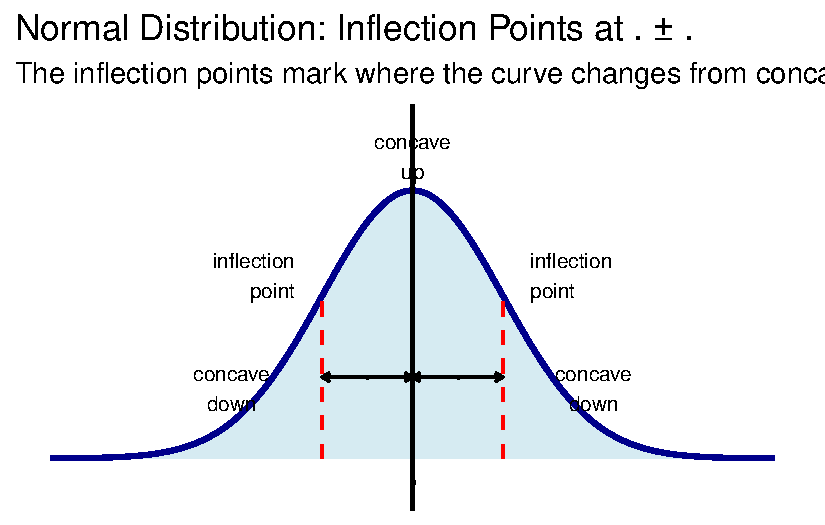
\includegraphics[keepaspectratio]{index_files/figure-pdf/unnamed-chunk-25-1.pdf}}

\begin{Shaded}
\begin{Highlighting}[]
\CommentTok{\# Optional: Add caption}
\CommentTok{\# + labs(caption = "We can find σ by eye at the inflection point of the density function of the normal distribution.")}
\end{Highlighting}
\end{Shaded}

\begin{Shaded}
\begin{Highlighting}[]
\NormalTok{fill\_green }\OtherTok{\textless{}{-}} \StringTok{"\#7FC97F"}
\NormalTok{fill\_yellow }\OtherTok{\textless{}{-}} \StringTok{"\#FFF59D"}
\NormalTok{curve\_blue }\OtherTok{\textless{}{-}} \StringTok{"\#2C7FB8"}
\NormalTok{panel\_blue }\OtherTok{\textless{}{-}} \StringTok{"\#DDEEFF"}
\NormalTok{grid\_major\_red }\OtherTok{\textless{}{-}} \StringTok{"\#F6C5C5"}
\NormalTok{grid\_minor\_red }\OtherTok{\textless{}{-}} \StringTok{"\#FBE6E6"}
\NormalTok{accent\_dark  }\OtherTok{\textless{}{-}} \StringTok{"\#1F4E79"}
\NormalTok{mean\_color   }\OtherTok{\textless{}{-}} \StringTok{"\#FF5733"}

\NormalTok{the\_theme\_big }\OtherTok{\textless{}{-}} \FunctionTok{theme\_minimal}\NormalTok{(}\AttributeTok{base\_size =} \DecValTok{18}\NormalTok{) }\SpecialCharTok{+}
  \FunctionTok{theme}\NormalTok{(}
    \AttributeTok{panel.background =} \FunctionTok{element\_rect}\NormalTok{(}\AttributeTok{fill =}\NormalTok{ panel\_blue, }\AttributeTok{color =} \ConstantTok{NA}\NormalTok{),}
    \AttributeTok{plot.background  =} \FunctionTok{element\_rect}\NormalTok{(}\AttributeTok{fill =} \StringTok{"white"}\NormalTok{, }\AttributeTok{color =} \ConstantTok{NA}\NormalTok{),}
    \AttributeTok{panel.grid.major =} \FunctionTok{element\_line}\NormalTok{(}\AttributeTok{color =}\NormalTok{ grid\_major\_red, }\AttributeTok{linewidth =} \FloatTok{0.6}\NormalTok{),}
    \AttributeTok{panel.grid.minor =} \FunctionTok{element\_line}\NormalTok{(}\AttributeTok{color =}\NormalTok{ grid\_minor\_red, }\AttributeTok{linewidth =} \FloatTok{0.35}\NormalTok{),}
    \AttributeTok{panel.grid.major.x =} \FunctionTok{element\_line}\NormalTok{(}\AttributeTok{color =}\NormalTok{ grid\_major\_red),}
    \AttributeTok{legend.position =} \StringTok{"none"}\NormalTok{,}
    \AttributeTok{plot.title =} \FunctionTok{element\_text}\NormalTok{(}\AttributeTok{face =} \StringTok{"bold"}\NormalTok{, }\AttributeTok{size =} \DecValTok{20}\NormalTok{),}
    \AttributeTok{axis.title =} \FunctionTok{element\_text}\NormalTok{(}\AttributeTok{size =} \DecValTok{18}\NormalTok{),}
    \AttributeTok{axis.text  =} \FunctionTok{element\_text}\NormalTok{(}\AttributeTok{size =} \DecValTok{14}\NormalTok{)}
\NormalTok{  )}

\NormalTok{x }\OtherTok{\textless{}{-}} \FunctionTok{seq}\NormalTok{(}\SpecialCharTok{{-}}\DecValTok{4}\NormalTok{,}\DecValTok{4}\NormalTok{,}\AttributeTok{length.out=}\DecValTok{2000}\NormalTok{)}
\NormalTok{y }\OtherTok{\textless{}{-}} \FunctionTok{dnorm}\NormalTok{(x,}\DecValTok{0}\NormalTok{,}\DecValTok{1}\NormalTok{)}
\NormalTok{df }\OtherTok{\textless{}{-}} \FunctionTok{data.frame}\NormalTok{(}\AttributeTok{x=}\NormalTok{x,}\AttributeTok{y=}\NormalTok{y)}
\NormalTok{ymax }\OtherTok{\textless{}{-}} \FunctionTok{max}\NormalTok{(y)}\SpecialCharTok{*}\FloatTok{1.12}

\NormalTok{df1 }\OtherTok{\textless{}{-}} \FunctionTok{subset}\NormalTok{(df, x}\SpecialCharTok{\textgreater{}={-}}\DecValTok{1} \SpecialCharTok{\&}\NormalTok{ x}\SpecialCharTok{\textless{}=}\DecValTok{1}\NormalTok{)}
\NormalTok{df2 }\OtherTok{\textless{}{-}} \FunctionTok{subset}\NormalTok{(df, x}\SpecialCharTok{\textgreater{}={-}}\DecValTok{2} \SpecialCharTok{\&}\NormalTok{ x}\SpecialCharTok{\textless{}=}\DecValTok{2}\NormalTok{)}
\NormalTok{df3 }\OtherTok{\textless{}{-}} \FunctionTok{subset}\NormalTok{(df, x}\SpecialCharTok{\textgreater{}={-}}\DecValTok{3} \SpecialCharTok{\&}\NormalTok{ x}\SpecialCharTok{\textless{}=}\DecValTok{3}\NormalTok{)}

\NormalTok{p\_rule }\OtherTok{\textless{}{-}} \FunctionTok{ggplot}\NormalTok{(df, }\FunctionTok{aes}\NormalTok{(x,y)) }\SpecialCharTok{+}
  \FunctionTok{geom\_area}\NormalTok{(}\AttributeTok{fill=}\NormalTok{fill\_green, }\AttributeTok{alpha=}\NormalTok{.}\DecValTok{5}\NormalTok{) }\SpecialCharTok{+}
  \FunctionTok{geom\_area}\NormalTok{(}\AttributeTok{data=}\NormalTok{df3, }\FunctionTok{aes}\NormalTok{(x,y), }\AttributeTok{fill=}\NormalTok{fill\_green, }\AttributeTok{alpha=}\NormalTok{.}\DecValTok{6}\NormalTok{) }\SpecialCharTok{+}
  \FunctionTok{geom\_area}\NormalTok{(}\AttributeTok{data=}\NormalTok{df2, }\FunctionTok{aes}\NormalTok{(x,y), }\AttributeTok{fill=}\NormalTok{fill\_yellow, }\AttributeTok{alpha=}\NormalTok{.}\DecValTok{9}\NormalTok{) }\SpecialCharTok{+}
  \FunctionTok{geom\_area}\NormalTok{(}\AttributeTok{data=}\NormalTok{df1, }\FunctionTok{aes}\NormalTok{(x,y), }\AttributeTok{fill=}\StringTok{"\#FFE066"}\NormalTok{, }\AttributeTok{alpha=}\NormalTok{.}\DecValTok{95}\NormalTok{) }\SpecialCharTok{+}
  \FunctionTok{geom\_line}\NormalTok{(}\AttributeTok{color=}\NormalTok{curve\_blue, }\AttributeTok{linewidth=}\FloatTok{1.8}\NormalTok{) }\SpecialCharTok{+}
  \FunctionTok{geom\_vline}\NormalTok{(}\AttributeTok{xintercept =} \FunctionTok{c}\NormalTok{(}\SpecialCharTok{{-}}\DecValTok{3}\NormalTok{,}\SpecialCharTok{{-}}\DecValTok{2}\NormalTok{,}\SpecialCharTok{{-}}\DecValTok{1}\NormalTok{,}\DecValTok{0}\NormalTok{,}\DecValTok{1}\NormalTok{,}\DecValTok{2}\NormalTok{,}\DecValTok{3}\NormalTok{), }\AttributeTok{linewidth=}\NormalTok{.}\DecValTok{7}\NormalTok{, }\AttributeTok{color=}\NormalTok{accent\_dark, }\AttributeTok{linetype=}\StringTok{"dotted"}\NormalTok{) }\SpecialCharTok{+}
  \FunctionTok{annotate}\NormalTok{(}\StringTok{"text"}\NormalTok{, }\AttributeTok{x=}\DecValTok{0}\NormalTok{, }\AttributeTok{y=}\NormalTok{ymax}\SpecialCharTok{*}\NormalTok{.}\DecValTok{93}\NormalTok{, }\AttributeTok{label=}\StringTok{"68\% within \textbackslash{}u00B11\textbackslash{}u03C3"}\NormalTok{, }\AttributeTok{fontface=}\StringTok{"bold"}\NormalTok{) }\SpecialCharTok{+}
  \FunctionTok{annotate}\NormalTok{(}\StringTok{"text"}\NormalTok{, }\AttributeTok{x=}\DecValTok{0}\NormalTok{, }\AttributeTok{y=}\NormalTok{ymax}\SpecialCharTok{*}\NormalTok{.}\DecValTok{85}\NormalTok{, }\AttributeTok{label=}\StringTok{"95\% within \textbackslash{}u00B12\textbackslash{}u03C3"}\NormalTok{, }\AttributeTok{fontface=}\StringTok{"bold"}\NormalTok{, }\AttributeTok{color=}\NormalTok{accent\_dark) }\SpecialCharTok{+}
  \FunctionTok{annotate}\NormalTok{(}\StringTok{"text"}\NormalTok{, }\AttributeTok{x=}\DecValTok{0}\NormalTok{, }\AttributeTok{y=}\NormalTok{ymax}\SpecialCharTok{*}\NormalTok{.}\DecValTok{77}\NormalTok{, }\AttributeTok{label=}\StringTok{"99.7\% within \textbackslash{}u00B13\textbackslash{}u03C3"}\NormalTok{, }\AttributeTok{fontface=}\StringTok{"bold"}\NormalTok{, }\AttributeTok{color=}\NormalTok{accent\_dark) }\SpecialCharTok{+}
  \FunctionTok{labs}\NormalTok{(}\AttributeTok{title=}\StringTok{"Normal distributions: the 68–95–99.7 rule"}\NormalTok{, }\AttributeTok{x=}\StringTok{"Standard deviations"}\NormalTok{, }\AttributeTok{y=}\StringTok{"Density"}\NormalTok{) }\SpecialCharTok{+}
  \FunctionTok{coord\_cartesian}\NormalTok{(}\AttributeTok{xlim=}\FunctionTok{c}\NormalTok{(}\SpecialCharTok{{-}}\FloatTok{3.5}\NormalTok{,}\FloatTok{3.5}\NormalTok{), }\AttributeTok{ylim=}\FunctionTok{c}\NormalTok{(}\DecValTok{0}\NormalTok{,ymax)) }\SpecialCharTok{+}
\NormalTok{  the\_theme\_big}

\NormalTok{xw }\OtherTok{\textless{}{-}} \FunctionTok{seq}\NormalTok{(}\DecValTok{54}\NormalTok{,}\DecValTok{75}\NormalTok{,}\AttributeTok{length.out=}\DecValTok{2000}\NormalTok{)}
\NormalTok{mu }\OtherTok{\textless{}{-}} \FloatTok{64.5}\NormalTok{; sigma }\OtherTok{\textless{}{-}} \FloatTok{2.5}
\NormalTok{yw }\OtherTok{\textless{}{-}} \FunctionTok{dnorm}\NormalTok{(xw,mu,sigma)}
\NormalTok{dfw }\OtherTok{\textless{}{-}} \FunctionTok{data.frame}\NormalTok{(}\AttributeTok{x=}\NormalTok{xw,}\AttributeTok{y=}\NormalTok{yw)}
\NormalTok{ymaxw }\OtherTok{\textless{}{-}} \FunctionTok{max}\NormalTok{(yw)}\SpecialCharTok{*}\FloatTok{1.12}
\NormalTok{shade1 }\OtherTok{\textless{}{-}} \FunctionTok{subset}\NormalTok{(dfw, x}\SpecialCharTok{\textgreater{}=}\NormalTok{mu}\SpecialCharTok{{-}}\NormalTok{sigma }\SpecialCharTok{\&}\NormalTok{ x}\SpecialCharTok{\textless{}=}\NormalTok{mu}\SpecialCharTok{+}\NormalTok{sigma)}

\NormalTok{p\_women }\OtherTok{\textless{}{-}} \FunctionTok{ggplot}\NormalTok{(dfw, }\FunctionTok{aes}\NormalTok{(x,y)) }\SpecialCharTok{+}
  \FunctionTok{geom\_area}\NormalTok{(}\AttributeTok{fill=}\NormalTok{fill\_green, }\AttributeTok{alpha=}\NormalTok{.}\DecValTok{6}\NormalTok{) }\SpecialCharTok{+}
  \FunctionTok{geom\_area}\NormalTok{(}\AttributeTok{data=}\NormalTok{shade1, }\FunctionTok{aes}\NormalTok{(x,y), }\AttributeTok{fill=}\NormalTok{fill\_yellow, }\AttributeTok{alpha=}\NormalTok{.}\DecValTok{95}\NormalTok{) }\SpecialCharTok{+}
  \FunctionTok{geom\_line}\NormalTok{(}\AttributeTok{color=}\NormalTok{curve\_blue, }\AttributeTok{linewidth=}\FloatTok{1.8}\NormalTok{) }\SpecialCharTok{+}
  \FunctionTok{geom\_vline}\NormalTok{(}\AttributeTok{xintercept =}\NormalTok{ mu, }\AttributeTok{color=}\NormalTok{mean\_color, }\AttributeTok{linewidth=}\FloatTok{1.6}\NormalTok{) }\SpecialCharTok{+}
  \FunctionTok{geom\_vline}\NormalTok{(}\AttributeTok{xintercept =} \FunctionTok{c}\NormalTok{(mu}\SpecialCharTok{{-}}\NormalTok{sigma, mu}\SpecialCharTok{+}\NormalTok{sigma), }\AttributeTok{color=}\NormalTok{accent\_dark, }\AttributeTok{linetype=}\StringTok{"dashed"}\NormalTok{) }\SpecialCharTok{+}
  \FunctionTok{annotate}\NormalTok{(}\StringTok{"text"}\NormalTok{, }\AttributeTok{x=}\NormalTok{mu, }\AttributeTok{y=}\NormalTok{ymaxw}\SpecialCharTok{*}\NormalTok{.}\DecValTok{06}\NormalTok{, }\AttributeTok{label=}\StringTok{"\textbackslash{}u03BC=64.5"}\NormalTok{, }\AttributeTok{color=}\NormalTok{mean\_color, }\AttributeTok{fontface=}\StringTok{"bold"}\NormalTok{) }\SpecialCharTok{+}
  \FunctionTok{annotate}\NormalTok{(}\StringTok{"text"}\NormalTok{, }\AttributeTok{x=}\NormalTok{mu}\FloatTok{{-}4.5}\NormalTok{, }\AttributeTok{y=}\NormalTok{ymaxw}\SpecialCharTok{*}\NormalTok{.}\DecValTok{92}\NormalTok{, }\AttributeTok{label=}\StringTok{"Inflection points at \textbackslash{}u03BC \textbackslash{}u00B1 \textbackslash{}u03C3"}\NormalTok{, }\AttributeTok{color=}\NormalTok{accent\_dark, }\AttributeTok{fontface=}\StringTok{"bold"}\NormalTok{, }\AttributeTok{hjust=}\DecValTok{0}\NormalTok{) }\SpecialCharTok{+}
  \FunctionTok{labs}\NormalTok{(}\AttributeTok{title=}\StringTok{"Distribution of heights of young women: N(64.5, 2.5)"}\NormalTok{, }\AttributeTok{x=}\StringTok{"Height (inches)"}\NormalTok{, }\AttributeTok{y=}\StringTok{"Density"}\NormalTok{) }\SpecialCharTok{+}
  \FunctionTok{coord\_cartesian}\NormalTok{(}\AttributeTok{ylim=}\FunctionTok{c}\NormalTok{(}\DecValTok{0}\NormalTok{,ymaxw)) }\SpecialCharTok{+}
\NormalTok{  the\_theme\_big}

\FunctionTok{grid.arrange}\NormalTok{(p\_rule, p\_women, }\AttributeTok{ncol=}\DecValTok{2}\NormalTok{)}
\end{Highlighting}
\end{Shaded}

\pandocbounded{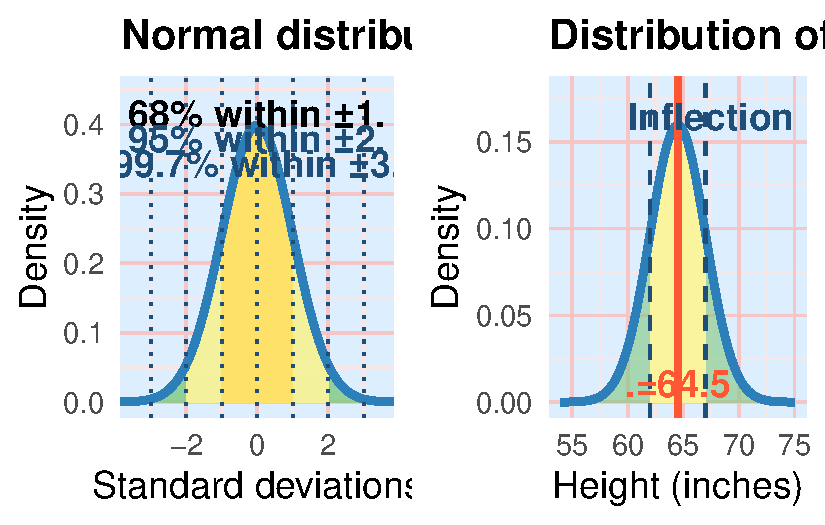
\includegraphics[keepaspectratio]{index_files/figure-pdf/unnamed-chunk-26-1.pdf}}

\begin{Shaded}
\begin{Highlighting}[]
 \FunctionTok{library}\NormalTok{(ggplot2)}
\FunctionTok{library}\NormalTok{(gridExtra)}
\FunctionTok{library}\NormalTok{(grid)}

\CommentTok{\# Color palette}
\NormalTok{fill\_green }\OtherTok{\textless{}{-}} \StringTok{"\#7FC97F"}
\NormalTok{fill\_yellow }\OtherTok{\textless{}{-}} \StringTok{"\#FFF59D"}
\NormalTok{fill\_orange }\OtherTok{\textless{}{-}} \StringTok{"\#FFE066"}
\NormalTok{curve\_blue }\OtherTok{\textless{}{-}} \StringTok{"\#2C7FB8"}
\NormalTok{panel\_blue }\OtherTok{\textless{}{-}} \StringTok{"\#DDEEFF"}
\NormalTok{grid\_major\_red }\OtherTok{\textless{}{-}} \StringTok{"\#F6C5C5"}
\NormalTok{grid\_minor\_red }\OtherTok{\textless{}{-}} \StringTok{"\#FBE6E6"}
\NormalTok{accent\_dark  }\OtherTok{\textless{}{-}} \StringTok{"\#1F4E79"}
\NormalTok{mean\_color   }\OtherTok{\textless{}{-}} \StringTok{"\#FF5733"}

\CommentTok{\# Consistent theme}
\NormalTok{the\_theme\_big }\OtherTok{\textless{}{-}} \FunctionTok{theme\_minimal}\NormalTok{(}\AttributeTok{base\_size =} \DecValTok{16}\NormalTok{) }\SpecialCharTok{+}
  \FunctionTok{theme}\NormalTok{(}
    \AttributeTok{panel.background =} \FunctionTok{element\_rect}\NormalTok{(}\AttributeTok{fill =}\NormalTok{ panel\_blue, }\AttributeTok{color =} \ConstantTok{NA}\NormalTok{),}
    \AttributeTok{plot.background  =} \FunctionTok{element\_rect}\NormalTok{(}\AttributeTok{fill =} \StringTok{"white"}\NormalTok{, }\AttributeTok{color =} \ConstantTok{NA}\NormalTok{),}
    \AttributeTok{panel.grid.major =} \FunctionTok{element\_line}\NormalTok{(}\AttributeTok{color =}\NormalTok{ grid\_major\_red, }\AttributeTok{linewidth =} \FloatTok{0.5}\NormalTok{),}
    \AttributeTok{panel.grid.minor =} \FunctionTok{element\_line}\NormalTok{(}\AttributeTok{color =}\NormalTok{ grid\_minor\_red, }\AttributeTok{linewidth =} \FloatTok{0.3}\NormalTok{),}
    \AttributeTok{panel.grid.major.x =} \FunctionTok{element\_line}\NormalTok{(}\AttributeTok{color =}\NormalTok{ grid\_major\_red),}
    \AttributeTok{legend.position =} \StringTok{"none"}\NormalTok{,}
    \AttributeTok{plot.title =} \FunctionTok{element\_text}\NormalTok{(}\AttributeTok{face =} \StringTok{"bold"}\NormalTok{, }\AttributeTok{size =} \DecValTok{18}\NormalTok{, }\AttributeTok{hjust =} \FloatTok{0.5}\NormalTok{),}
    \AttributeTok{axis.title =} \FunctionTok{element\_text}\NormalTok{(}\AttributeTok{size =} \DecValTok{15}\NormalTok{, }\AttributeTok{face =} \StringTok{"bold"}\NormalTok{),}
    \AttributeTok{axis.text  =} \FunctionTok{element\_text}\NormalTok{(}\AttributeTok{size =} \DecValTok{13}\NormalTok{)}
\NormalTok{  )}

\CommentTok{\# {-}{-}{-}{-}{-}{-}{-}{-}{-}{-} PLOT 1: 68{-}95{-}99.7 Rule {-}{-}{-}{-}{-}{-}{-}{-}{-}{-}}
\NormalTok{x }\OtherTok{\textless{}{-}} \FunctionTok{seq}\NormalTok{(}\SpecialCharTok{{-}}\DecValTok{4}\NormalTok{, }\DecValTok{4}\NormalTok{, }\AttributeTok{length.out =} \DecValTok{2000}\NormalTok{)}
\NormalTok{y }\OtherTok{\textless{}{-}} \FunctionTok{dnorm}\NormalTok{(x, }\DecValTok{0}\NormalTok{, }\DecValTok{1}\NormalTok{)}
\NormalTok{df }\OtherTok{\textless{}{-}} \FunctionTok{data.frame}\NormalTok{(}\AttributeTok{x =}\NormalTok{ x, }\AttributeTok{y =}\NormalTok{ y)}
\NormalTok{ymax }\OtherTok{\textless{}{-}} \FunctionTok{max}\NormalTok{(y) }\SpecialCharTok{*} \FloatTok{1.15}

\CommentTok{\# Create shaded regions}
\NormalTok{df1 }\OtherTok{\textless{}{-}} \FunctionTok{subset}\NormalTok{(df, x }\SpecialCharTok{\textgreater{}=} \SpecialCharTok{{-}}\DecValTok{1} \SpecialCharTok{\&}\NormalTok{ x }\SpecialCharTok{\textless{}=} \DecValTok{1}\NormalTok{)}
\NormalTok{df2 }\OtherTok{\textless{}{-}} \FunctionTok{subset}\NormalTok{(df, x }\SpecialCharTok{\textgreater{}=} \SpecialCharTok{{-}}\DecValTok{2} \SpecialCharTok{\&}\NormalTok{ x }\SpecialCharTok{\textless{}=} \DecValTok{2}\NormalTok{)}
\NormalTok{df3 }\OtherTok{\textless{}{-}} \FunctionTok{subset}\NormalTok{(df, x }\SpecialCharTok{\textgreater{}=} \SpecialCharTok{{-}}\DecValTok{3} \SpecialCharTok{\&}\NormalTok{ x }\SpecialCharTok{\textless{}=} \DecValTok{3}\NormalTok{)}

\NormalTok{p\_rule }\OtherTok{\textless{}{-}} \FunctionTok{ggplot}\NormalTok{(df, }\FunctionTok{aes}\NormalTok{(x, y)) }\SpecialCharTok{+}
  \CommentTok{\# Layered shading for visual effect}
  \FunctionTok{geom\_area}\NormalTok{(}\AttributeTok{fill =}\NormalTok{ fill\_green, }\AttributeTok{alpha =} \FloatTok{0.4}\NormalTok{) }\SpecialCharTok{+}
  \FunctionTok{geom\_area}\NormalTok{(}\AttributeTok{data =}\NormalTok{ df3, }\FunctionTok{aes}\NormalTok{(x, y), }\AttributeTok{fill =}\NormalTok{ fill\_green, }\AttributeTok{alpha =} \FloatTok{0.5}\NormalTok{) }\SpecialCharTok{+}
  \FunctionTok{geom\_area}\NormalTok{(}\AttributeTok{data =}\NormalTok{ df2, }\FunctionTok{aes}\NormalTok{(x, y), }\AttributeTok{fill =}\NormalTok{ fill\_yellow, }\AttributeTok{alpha =} \FloatTok{0.85}\NormalTok{) }\SpecialCharTok{+}
  \FunctionTok{geom\_area}\NormalTok{(}\AttributeTok{data =}\NormalTok{ df1, }\FunctionTok{aes}\NormalTok{(x, y), }\AttributeTok{fill =}\NormalTok{ fill\_orange, }\AttributeTok{alpha =} \FloatTok{0.9}\NormalTok{) }\SpecialCharTok{+}
  
  \CommentTok{\# Main curve}
  \FunctionTok{geom\_line}\NormalTok{(}\AttributeTok{color =}\NormalTok{ curve\_blue, }\AttributeTok{linewidth =} \DecValTok{2}\NormalTok{) }\SpecialCharTok{+}
  
  \CommentTok{\# Vertical lines at standard deviations}
  \FunctionTok{geom\_vline}\NormalTok{(}\AttributeTok{xintercept =} \FunctionTok{c}\NormalTok{(}\SpecialCharTok{{-}}\DecValTok{3}\NormalTok{, }\SpecialCharTok{{-}}\DecValTok{2}\NormalTok{, }\SpecialCharTok{{-}}\DecValTok{1}\NormalTok{, }\DecValTok{0}\NormalTok{, }\DecValTok{1}\NormalTok{, }\DecValTok{2}\NormalTok{, }\DecValTok{3}\NormalTok{), }
             \AttributeTok{linewidth =} \FloatTok{0.8}\NormalTok{, }\AttributeTok{color =}\NormalTok{ accent\_dark, }\AttributeTok{linetype =} \StringTok{"dotted"}\NormalTok{) }\SpecialCharTok{+}
  
  \CommentTok{\# Labels for percentages}
  \FunctionTok{annotate}\NormalTok{(}\StringTok{"text"}\NormalTok{, }\AttributeTok{x =} \DecValTok{0}\NormalTok{, }\AttributeTok{y =}\NormalTok{ ymax }\SpecialCharTok{*} \FloatTok{0.94}\NormalTok{, }
           \AttributeTok{label =} \StringTok{"68\% within ±1σ"}\NormalTok{, }
           \AttributeTok{fontface =} \StringTok{"bold"}\NormalTok{, }\AttributeTok{size =} \FloatTok{5.5}\NormalTok{) }\SpecialCharTok{+}
  \FunctionTok{annotate}\NormalTok{(}\StringTok{"text"}\NormalTok{, }\AttributeTok{x =} \DecValTok{0}\NormalTok{, }\AttributeTok{y =}\NormalTok{ ymax }\SpecialCharTok{*} \FloatTok{0.86}\NormalTok{, }
           \AttributeTok{label =} \StringTok{"95\% within ±2σ"}\NormalTok{, }
           \AttributeTok{fontface =} \StringTok{"bold"}\NormalTok{, }\AttributeTok{size =} \FloatTok{5.5}\NormalTok{, }\AttributeTok{color =}\NormalTok{ accent\_dark) }\SpecialCharTok{+}
  \FunctionTok{annotate}\NormalTok{(}\StringTok{"text"}\NormalTok{, }\AttributeTok{x =} \DecValTok{0}\NormalTok{, }\AttributeTok{y =}\NormalTok{ ymax }\SpecialCharTok{*} \FloatTok{0.78}\NormalTok{, }
           \AttributeTok{label =} \StringTok{"99.7\% within ±3σ"}\NormalTok{, }
           \AttributeTok{fontface =} \StringTok{"bold"}\NormalTok{, }\AttributeTok{size =} \FloatTok{5.5}\NormalTok{, }\AttributeTok{color =}\NormalTok{ accent\_dark) }\SpecialCharTok{+}
  
  \CommentTok{\# Axis labels at key points}
  \FunctionTok{scale\_x\_continuous}\NormalTok{(}\AttributeTok{breaks =} \FunctionTok{c}\NormalTok{(}\SpecialCharTok{{-}}\DecValTok{3}\NormalTok{, }\SpecialCharTok{{-}}\DecValTok{2}\NormalTok{, }\SpecialCharTok{{-}}\DecValTok{1}\NormalTok{, }\DecValTok{0}\NormalTok{, }\DecValTok{1}\NormalTok{, }\DecValTok{2}\NormalTok{, }\DecValTok{3}\NormalTok{),}
                     \AttributeTok{labels =} \FunctionTok{c}\NormalTok{(}\StringTok{"{-}3σ"}\NormalTok{, }\StringTok{"{-}2σ"}\NormalTok{, }\StringTok{"{-}1σ"}\NormalTok{, }\StringTok{"μ"}\NormalTok{, }\StringTok{"+1σ"}\NormalTok{, }\StringTok{"+2σ"}\NormalTok{, }\StringTok{"+3σ"}\NormalTok{)) }\SpecialCharTok{+}
  
  \FunctionTok{labs}\NormalTok{(}\AttributeTok{title =} \StringTok{"The 68–95–99.7 Rule for Normal Distributions"}\NormalTok{, }
       \AttributeTok{x =} \StringTok{"Standard Deviations from Mean"}\NormalTok{, }
       \AttributeTok{y =} \StringTok{"Density"}\NormalTok{) }\SpecialCharTok{+}
  
  \FunctionTok{coord\_cartesian}\NormalTok{(}\AttributeTok{xlim =} \FunctionTok{c}\NormalTok{(}\SpecialCharTok{{-}}\FloatTok{3.8}\NormalTok{, }\FloatTok{3.8}\NormalTok{), }\AttributeTok{ylim =} \FunctionTok{c}\NormalTok{(}\DecValTok{0}\NormalTok{, ymax)) }\SpecialCharTok{+}
\NormalTok{  the\_theme\_big}

\CommentTok{\# {-}{-}{-}{-}{-}{-}{-}{-}{-}{-} PLOT 2: Women\textquotesingle{}s Heights {-}{-}{-}{-}{-}{-}{-}{-}{-}{-}}
\NormalTok{xw }\OtherTok{\textless{}{-}} \FunctionTok{seq}\NormalTok{(}\DecValTok{56}\NormalTok{, }\DecValTok{73}\NormalTok{, }\AttributeTok{length.out =} \DecValTok{2000}\NormalTok{)}
\NormalTok{mu }\OtherTok{\textless{}{-}} \FloatTok{64.5}
\NormalTok{sigma }\OtherTok{\textless{}{-}} \FloatTok{2.5}
\NormalTok{yw }\OtherTok{\textless{}{-}} \FunctionTok{dnorm}\NormalTok{(xw, mu, sigma)}
\NormalTok{dfw }\OtherTok{\textless{}{-}} \FunctionTok{data.frame}\NormalTok{(}\AttributeTok{x =}\NormalTok{ xw, }\AttributeTok{y =}\NormalTok{ yw)}
\NormalTok{ymaxw }\OtherTok{\textless{}{-}} \FunctionTok{max}\NormalTok{(yw) }\SpecialCharTok{*} \FloatTok{1.15}

\CommentTok{\# Shaded regions}
\NormalTok{shade1 }\OtherTok{\textless{}{-}} \FunctionTok{subset}\NormalTok{(dfw, x }\SpecialCharTok{\textgreater{}=}\NormalTok{ mu }\SpecialCharTok{{-}}\NormalTok{ sigma }\SpecialCharTok{\&}\NormalTok{ x }\SpecialCharTok{\textless{}=}\NormalTok{ mu }\SpecialCharTok{+}\NormalTok{ sigma)}
\NormalTok{shade2 }\OtherTok{\textless{}{-}} \FunctionTok{subset}\NormalTok{(dfw, x }\SpecialCharTok{\textgreater{}=}\NormalTok{ mu }\SpecialCharTok{{-}} \DecValTok{2}\SpecialCharTok{*}\NormalTok{sigma }\SpecialCharTok{\&}\NormalTok{ x }\SpecialCharTok{\textless{}=}\NormalTok{ mu }\SpecialCharTok{+} \DecValTok{2}\SpecialCharTok{*}\NormalTok{sigma)}

\NormalTok{p\_women }\OtherTok{\textless{}{-}} \FunctionTok{ggplot}\NormalTok{(dfw, }\FunctionTok{aes}\NormalTok{(x, y)) }\SpecialCharTok{+}
  \CommentTok{\# Shading}
  \FunctionTok{geom\_area}\NormalTok{(}\AttributeTok{fill =}\NormalTok{ fill\_green, }\AttributeTok{alpha =} \FloatTok{0.5}\NormalTok{) }\SpecialCharTok{+}
  \FunctionTok{geom\_area}\NormalTok{(}\AttributeTok{data =}\NormalTok{ shade2, }\FunctionTok{aes}\NormalTok{(x, y), }\AttributeTok{fill =}\NormalTok{ fill\_yellow, }\AttributeTok{alpha =} \FloatTok{0.7}\NormalTok{) }\SpecialCharTok{+}
  \FunctionTok{geom\_area}\NormalTok{(}\AttributeTok{data =}\NormalTok{ shade1, }\FunctionTok{aes}\NormalTok{(x, y), }\AttributeTok{fill =}\NormalTok{ fill\_orange, }\AttributeTok{alpha =} \FloatTok{0.9}\NormalTok{) }\SpecialCharTok{+}
  
  \CommentTok{\# Main curve}
  \FunctionTok{geom\_line}\NormalTok{(}\AttributeTok{color =}\NormalTok{ curve\_blue, }\AttributeTok{linewidth =} \DecValTok{2}\NormalTok{) }\SpecialCharTok{+}
  
  \CommentTok{\# Mean line}
  \FunctionTok{geom\_vline}\NormalTok{(}\AttributeTok{xintercept =}\NormalTok{ mu, }\AttributeTok{color =}\NormalTok{ mean\_color, }\AttributeTok{linewidth =} \FloatTok{1.8}\NormalTok{) }\SpecialCharTok{+}
  
  \CommentTok{\# Inflection points}
  \FunctionTok{geom\_vline}\NormalTok{(}\AttributeTok{xintercept =} \FunctionTok{c}\NormalTok{(mu }\SpecialCharTok{{-}}\NormalTok{ sigma, mu }\SpecialCharTok{+}\NormalTok{ sigma), }
             \AttributeTok{color =}\NormalTok{ accent\_dark, }\AttributeTok{linetype =} \StringTok{"dashed"}\NormalTok{, }\AttributeTok{linewidth =} \DecValTok{1}\NormalTok{) }\SpecialCharTok{+}
  
  \CommentTok{\# Labels}
  \FunctionTok{annotate}\NormalTok{(}\StringTok{"text"}\NormalTok{, }\AttributeTok{x =}\NormalTok{ mu, }\AttributeTok{y =}\NormalTok{ ymaxw }\SpecialCharTok{*} \FloatTok{0.08}\NormalTok{, }
           \AttributeTok{label =} \FunctionTok{paste0}\NormalTok{(}\StringTok{"μ = "}\NormalTok{, mu, }\StringTok{" inches"}\NormalTok{), }
           \AttributeTok{color =}\NormalTok{ mean\_color, }\AttributeTok{fontface =} \StringTok{"bold"}\NormalTok{, }\AttributeTok{size =} \DecValTok{5}\NormalTok{) }\SpecialCharTok{+}
  
  \FunctionTok{annotate}\NormalTok{(}\StringTok{"text"}\NormalTok{, }\AttributeTok{x =}\NormalTok{ mu }\SpecialCharTok{{-}}\NormalTok{ sigma, }\AttributeTok{y =}\NormalTok{ ymaxw }\SpecialCharTok{*} \FloatTok{0.96}\NormalTok{, }
           \AttributeTok{label =} \StringTok{"Inflection points at μ ± σ"}\NormalTok{, }
           \AttributeTok{color =}\NormalTok{ accent\_dark, }\AttributeTok{fontface =} \StringTok{"bold"}\NormalTok{, }\AttributeTok{size =} \FloatTok{4.5}\NormalTok{) }\SpecialCharTok{+}
  
  \FunctionTok{annotate}\NormalTok{(}\StringTok{"segment"}\NormalTok{, }\AttributeTok{x =}\NormalTok{ mu }\SpecialCharTok{{-}}\NormalTok{ sigma }\SpecialCharTok{{-}} \FloatTok{0.3}\NormalTok{, }\AttributeTok{xend =}\NormalTok{ mu }\SpecialCharTok{{-}}\NormalTok{ sigma, }
           \AttributeTok{y =}\NormalTok{ ymaxw }\SpecialCharTok{*} \FloatTok{0.93}\NormalTok{, }\AttributeTok{yend =} \FunctionTok{dnorm}\NormalTok{(mu }\SpecialCharTok{{-}}\NormalTok{ sigma, mu, sigma) }\SpecialCharTok{+} \FloatTok{0.003}\NormalTok{,}
           \AttributeTok{arrow =} \FunctionTok{arrow}\NormalTok{(}\AttributeTok{length =} \FunctionTok{unit}\NormalTok{(}\FloatTok{0.2}\NormalTok{, }\StringTok{"cm"}\NormalTok{)), }
           \AttributeTok{color =}\NormalTok{ accent\_dark, }\AttributeTok{linewidth =} \FloatTok{0.8}\NormalTok{) }\SpecialCharTok{+}
  
  \FunctionTok{annotate}\NormalTok{(}\StringTok{"segment"}\NormalTok{, }\AttributeTok{x =}\NormalTok{ mu }\SpecialCharTok{+}\NormalTok{ sigma }\SpecialCharTok{+} \FloatTok{0.3}\NormalTok{, }\AttributeTok{xend =}\NormalTok{ mu }\SpecialCharTok{+}\NormalTok{ sigma, }
           \AttributeTok{y =}\NormalTok{ ymaxw }\SpecialCharTok{*} \FloatTok{0.93}\NormalTok{, }\AttributeTok{yend =} \FunctionTok{dnorm}\NormalTok{(mu }\SpecialCharTok{+}\NormalTok{ sigma, mu, sigma) }\SpecialCharTok{+} \FloatTok{0.003}\NormalTok{,}
           \AttributeTok{arrow =} \FunctionTok{arrow}\NormalTok{(}\AttributeTok{length =} \FunctionTok{unit}\NormalTok{(}\FloatTok{0.2}\NormalTok{, }\StringTok{"cm"}\NormalTok{)), }
           \AttributeTok{color =}\NormalTok{ accent\_dark, }\AttributeTok{linewidth =} \FloatTok{0.8}\NormalTok{) }\SpecialCharTok{+}
  
  \CommentTok{\# Percentage label}
  \FunctionTok{annotate}\NormalTok{(}\StringTok{"text"}\NormalTok{, }\AttributeTok{x =}\NormalTok{ mu, }\AttributeTok{y =}\NormalTok{ ymaxw }\SpecialCharTok{*} \FloatTok{0.45}\NormalTok{, }
           \AttributeTok{label =} \StringTok{"68\%"}\NormalTok{, }\AttributeTok{fontface =} \StringTok{"bold"}\NormalTok{, }\AttributeTok{size =} \DecValTok{6}\NormalTok{, }\AttributeTok{color =}\NormalTok{ accent\_dark) }\SpecialCharTok{+}
  
  \FunctionTok{labs}\NormalTok{(}\AttributeTok{title =} \StringTok{"Distribution of Young Men\textquotesingle{}s Heights: N(64.5, 2.5)"}\NormalTok{, }
       \AttributeTok{x =} \StringTok{"Height (inches)"}\NormalTok{, }
       \AttributeTok{y =} \StringTok{"Density"}\NormalTok{) }\SpecialCharTok{+}
  
  \FunctionTok{scale\_x\_continuous}\NormalTok{(}\AttributeTok{breaks =} \FunctionTok{seq}\NormalTok{(}\DecValTok{58}\NormalTok{, }\DecValTok{72}\NormalTok{, }\AttributeTok{by =} \DecValTok{2}\NormalTok{)) }\SpecialCharTok{+}
  
  \FunctionTok{coord\_cartesian}\NormalTok{(}\AttributeTok{xlim =} \FunctionTok{c}\NormalTok{(}\DecValTok{56}\NormalTok{, }\DecValTok{73}\NormalTok{), }\AttributeTok{ylim =} \FunctionTok{c}\NormalTok{(}\DecValTok{0}\NormalTok{, ymaxw)) }\SpecialCharTok{+}
\NormalTok{  the\_theme\_big}

\CommentTok{\# Display both plots}
\FunctionTok{grid.arrange}\NormalTok{(p\_rule, p\_women, }\AttributeTok{ncol =} \DecValTok{2}\NormalTok{,}
             \AttributeTok{top =} \FunctionTok{textGrob}\NormalTok{(}\StringTok{"Understanding the Normal Distribution"}\NormalTok{,}
                           \AttributeTok{gp =} \FunctionTok{gpar}\NormalTok{(}\AttributeTok{fontsize =} \DecValTok{20}\NormalTok{, }\AttributeTok{fontface =} \StringTok{"bold"}\NormalTok{)))}
\end{Highlighting}
\end{Shaded}

\pandocbounded{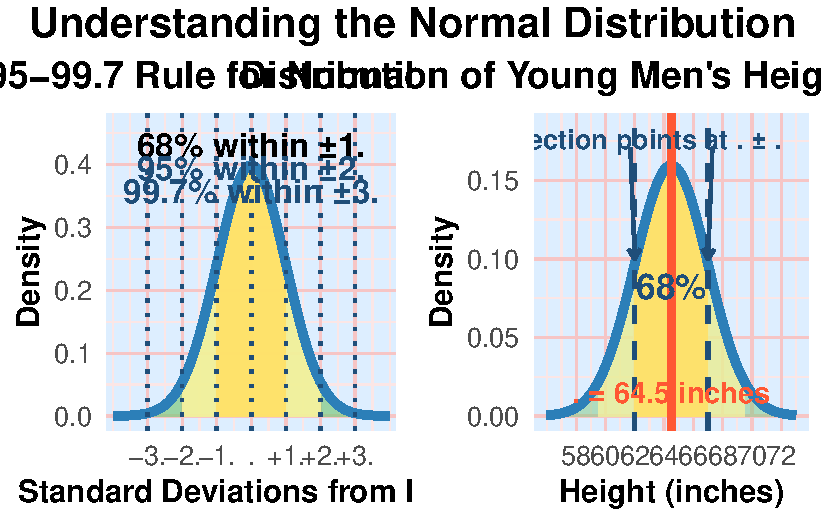
\includegraphics[keepaspectratio]{index_files/figure-pdf/unnamed-chunk-27-1.pdf}}

\begin{Shaded}
\begin{Highlighting}[]
\FunctionTok{library}\NormalTok{(ggplot2)}
\FunctionTok{library}\NormalTok{(gridExtra)}
\FunctionTok{library}\NormalTok{(grid)}

\CommentTok{\# Color palette}
\NormalTok{fill\_green }\OtherTok{\textless{}{-}} \StringTok{"\#7FC97F"}
\NormalTok{fill\_yellow }\OtherTok{\textless{}{-}} \StringTok{"\#FFF59D"}
\NormalTok{curve\_blue }\OtherTok{\textless{}{-}} \StringTok{"\#2C7FB8"}
\NormalTok{panel\_blue }\OtherTok{\textless{}{-}} \StringTok{"\#DDEEFF"}
\NormalTok{grid\_major\_red }\OtherTok{\textless{}{-}} \StringTok{"\#F6C5C5"}
\NormalTok{grid\_minor\_red }\OtherTok{\textless{}{-}} \StringTok{"\#FBE6E6"}
\NormalTok{accent\_dark  }\OtherTok{\textless{}{-}} \StringTok{"\#1F4E79"}
\NormalTok{mean\_color   }\OtherTok{\textless{}{-}} \StringTok{"\#FF5733"}

\CommentTok{\# Theme}
\NormalTok{the\_theme\_big }\OtherTok{\textless{}{-}} \FunctionTok{theme\_minimal}\NormalTok{(}\AttributeTok{base\_size =} \DecValTok{16}\NormalTok{) }\SpecialCharTok{+}
  \FunctionTok{theme}\NormalTok{(}
    \AttributeTok{panel.background =} \FunctionTok{element\_rect}\NormalTok{(}\AttributeTok{fill =}\NormalTok{ panel\_blue, }\AttributeTok{color =} \ConstantTok{NA}\NormalTok{),}
    \AttributeTok{plot.background  =} \FunctionTok{element\_rect}\NormalTok{(}\AttributeTok{fill =} \StringTok{"white"}\NormalTok{, }\AttributeTok{color =} \ConstantTok{NA}\NormalTok{),}
    \AttributeTok{panel.grid.major =} \FunctionTok{element\_line}\NormalTok{(}\AttributeTok{color =}\NormalTok{ grid\_major\_red, }\AttributeTok{linewidth =} \FloatTok{0.5}\NormalTok{),}
    \AttributeTok{panel.grid.minor =} \FunctionTok{element\_line}\NormalTok{(}\AttributeTok{color =}\NormalTok{ grid\_minor\_red, }\AttributeTok{linewidth =} \FloatTok{0.3}\NormalTok{),}
    \AttributeTok{panel.grid.major.x =} \FunctionTok{element\_line}\NormalTok{(}\AttributeTok{color =}\NormalTok{ grid\_major\_red),}
    \AttributeTok{legend.position =} \StringTok{"none"}\NormalTok{,}
    \AttributeTok{plot.title =} \FunctionTok{element\_text}\NormalTok{(}\AttributeTok{face =} \StringTok{"bold"}\NormalTok{, }\AttributeTok{size =} \DecValTok{17}\NormalTok{, }\AttributeTok{hjust =} \FloatTok{0.5}\NormalTok{),}
    \AttributeTok{plot.subtitle =} \FunctionTok{element\_text}\NormalTok{(}\AttributeTok{size =} \DecValTok{13}\NormalTok{, }\AttributeTok{hjust =} \FloatTok{0.5}\NormalTok{, }\AttributeTok{color =}\NormalTok{ accent\_dark),}
    \AttributeTok{axis.title =} \FunctionTok{element\_text}\NormalTok{(}\AttributeTok{size =} \DecValTok{14}\NormalTok{, }\AttributeTok{face =} \StringTok{"bold"}\NormalTok{),}
    \AttributeTok{axis.text  =} \FunctionTok{element\_text}\NormalTok{(}\AttributeTok{size =} \DecValTok{12}\NormalTok{)}
\NormalTok{  )}

\CommentTok{\# Parameters}
\NormalTok{mu }\OtherTok{\textless{}{-}} \FloatTok{64.5}
\NormalTok{sigma }\OtherTok{\textless{}{-}} \FloatTok{2.5}
\NormalTok{x }\OtherTok{\textless{}{-}} \FunctionTok{seq}\NormalTok{(}\DecValTok{54}\NormalTok{, }\DecValTok{75}\NormalTok{, }\AttributeTok{length.out =} \DecValTok{2000}\NormalTok{)}
\NormalTok{y }\OtherTok{\textless{}{-}} \FunctionTok{dnorm}\NormalTok{(x, mu, sigma)}
\NormalTok{df }\OtherTok{\textless{}{-}} \FunctionTok{data.frame}\NormalTok{(}\AttributeTok{x =}\NormalTok{ x, }\AttributeTok{y =}\NormalTok{ y)}
\NormalTok{ymax }\OtherTok{\textless{}{-}} \FunctionTok{max}\NormalTok{(y) }\SpecialCharTok{*} \FloatTok{1.12}

\CommentTok{\# {-}{-}{-}{-}{-}{-}{-}{-}{-}{-} PLOT 1: Both Tails {-}{-}{-}{-}{-}{-}{-}{-}{-}{-}}
\NormalTok{shade\_both }\OtherTok{\textless{}{-}} \FunctionTok{subset}\NormalTok{(df, x }\SpecialCharTok{\textless{}=} \DecValTok{57} \SpecialCharTok{|}\NormalTok{ x }\SpecialCharTok{\textgreater{}=} \DecValTok{72}\NormalTok{)}
\NormalTok{prob\_both }\OtherTok{\textless{}{-}} \FunctionTok{pnorm}\NormalTok{(}\DecValTok{57}\NormalTok{, mu, sigma) }\SpecialCharTok{+}\NormalTok{ (}\DecValTok{1} \SpecialCharTok{{-}} \FunctionTok{pnorm}\NormalTok{(}\DecValTok{72}\NormalTok{, mu, sigma))}

\NormalTok{p\_both\_tails }\OtherTok{\textless{}{-}} \FunctionTok{ggplot}\NormalTok{(df, }\FunctionTok{aes}\NormalTok{(x, y)) }\SpecialCharTok{+}
  \FunctionTok{geom\_area}\NormalTok{(}\AttributeTok{fill =}\NormalTok{ fill\_green, }\AttributeTok{alpha =} \FloatTok{0.6}\NormalTok{) }\SpecialCharTok{+}
  \FunctionTok{geom\_area}\NormalTok{(}\AttributeTok{data =}\NormalTok{ shade\_both, }\FunctionTok{aes}\NormalTok{(x, y), }\AttributeTok{fill =}\NormalTok{ fill\_yellow, }\AttributeTok{alpha =} \FloatTok{0.95}\NormalTok{) }\SpecialCharTok{+}
  \FunctionTok{geom\_line}\NormalTok{(}\AttributeTok{color =}\NormalTok{ curve\_blue, }\AttributeTok{linewidth =} \DecValTok{2}\NormalTok{) }\SpecialCharTok{+}
  \FunctionTok{geom\_vline}\NormalTok{(}\AttributeTok{xintercept =}\NormalTok{ mu, }\AttributeTok{color =}\NormalTok{ mean\_color, }\AttributeTok{linewidth =} \FloatTok{1.8}\NormalTok{) }\SpecialCharTok{+}
  \FunctionTok{geom\_vline}\NormalTok{(}\AttributeTok{xintercept =} \FunctionTok{c}\NormalTok{(}\DecValTok{57}\NormalTok{, }\DecValTok{72}\NormalTok{), }\AttributeTok{color =}\NormalTok{ accent\_dark, }
             \AttributeTok{linetype =} \StringTok{"dashed"}\NormalTok{, }\AttributeTok{linewidth =} \DecValTok{1}\NormalTok{) }\SpecialCharTok{+}
  \FunctionTok{annotate}\NormalTok{(}\StringTok{"text"}\NormalTok{, }\AttributeTok{x =} \DecValTok{57}\NormalTok{, }\AttributeTok{y =}\NormalTok{ ymax }\SpecialCharTok{*} \FloatTok{0.95}\NormalTok{, }\AttributeTok{label =} \StringTok{"57}\SpecialCharTok{\textbackslash{}"}\StringTok{"}\NormalTok{, }
           \AttributeTok{color =}\NormalTok{ accent\_dark, }\AttributeTok{fontface =} \StringTok{"bold"}\NormalTok{, }\AttributeTok{size =} \FloatTok{4.5}\NormalTok{) }\SpecialCharTok{+}
  \FunctionTok{annotate}\NormalTok{(}\StringTok{"text"}\NormalTok{, }\AttributeTok{x =} \DecValTok{72}\NormalTok{, }\AttributeTok{y =}\NormalTok{ ymax }\SpecialCharTok{*} \FloatTok{0.95}\NormalTok{, }\AttributeTok{label =} \StringTok{"72}\SpecialCharTok{\textbackslash{}"}\StringTok{"}\NormalTok{, }
           \AttributeTok{color =}\NormalTok{ accent\_dark, }\AttributeTok{fontface =} \StringTok{"bold"}\NormalTok{, }\AttributeTok{size =} \FloatTok{4.5}\NormalTok{) }\SpecialCharTok{+}
  \FunctionTok{annotate}\NormalTok{(}\StringTok{"text"}\NormalTok{, }\AttributeTok{x =} \FloatTok{55.5}\NormalTok{, }\AttributeTok{y =}\NormalTok{ ymax }\SpecialCharTok{*} \FloatTok{0.15}\NormalTok{, }
           \AttributeTok{label =} \FunctionTok{sprintf}\NormalTok{(}\StringTok{"\%.4f"}\NormalTok{, }\FunctionTok{pnorm}\NormalTok{(}\DecValTok{57}\NormalTok{, mu, sigma)), }
           \AttributeTok{color =}\NormalTok{ accent\_dark, }\AttributeTok{fontface =} \StringTok{"bold"}\NormalTok{, }\AttributeTok{size =} \DecValTok{4}\NormalTok{) }\SpecialCharTok{+}
  \FunctionTok{annotate}\NormalTok{(}\StringTok{"text"}\NormalTok{, }\AttributeTok{x =} \FloatTok{73.5}\NormalTok{, }\AttributeTok{y =}\NormalTok{ ymax }\SpecialCharTok{*} \FloatTok{0.15}\NormalTok{, }
           \AttributeTok{label =} \FunctionTok{sprintf}\NormalTok{(}\StringTok{"\%.4f"}\NormalTok{, }\DecValTok{1} \SpecialCharTok{{-}} \FunctionTok{pnorm}\NormalTok{(}\DecValTok{72}\NormalTok{, mu, sigma)), }
           \AttributeTok{color =}\NormalTok{ accent\_dark, }\AttributeTok{fontface =} \StringTok{"bold"}\NormalTok{, }\AttributeTok{size =} \DecValTok{4}\NormalTok{) }\SpecialCharTok{+}
  \FunctionTok{labs}\NormalTok{(}
    \AttributeTok{title =} \StringTok{"Less than 57}\SpecialCharTok{\textbackslash{}"}\StringTok{ or more than 72}\SpecialCharTok{\textbackslash{}"}\StringTok{"}\NormalTok{,}
    \AttributeTok{subtitle =} \FunctionTok{paste0}\NormalTok{(}\StringTok{"≈ 0.003 by 68–95–99.7 rule; exact = "}\NormalTok{, }\FunctionTok{sprintf}\NormalTok{(}\StringTok{\textquotesingle{}\%.4f\textquotesingle{}}\NormalTok{, prob\_both)),}
    \AttributeTok{x =} \StringTok{"Height (inches)"}\NormalTok{, }\AttributeTok{y =} \StringTok{"Density"}
\NormalTok{  ) }\SpecialCharTok{+}
  \FunctionTok{coord\_cartesian}\NormalTok{(}\AttributeTok{ylim =} \FunctionTok{c}\NormalTok{(}\DecValTok{0}\NormalTok{, ymax)) }\SpecialCharTok{+}
\NormalTok{  the\_theme\_big}

\CommentTok{\# {-}{-}{-}{-}{-}{-}{-}{-}{-}{-} PLOT 2: Right Tail {-}{-}{-}{-}{-}{-}{-}{-}{-}{-}}
\NormalTok{shade\_right }\OtherTok{\textless{}{-}} \FunctionTok{subset}\NormalTok{(df, x }\SpecialCharTok{\textgreater{}=} \DecValTok{72}\NormalTok{)}
\NormalTok{prob\_right }\OtherTok{\textless{}{-}} \DecValTok{1} \SpecialCharTok{{-}} \FunctionTok{pnorm}\NormalTok{(}\DecValTok{72}\NormalTok{, mu, sigma)}

\NormalTok{p\_right\_tail }\OtherTok{\textless{}{-}} \FunctionTok{ggplot}\NormalTok{(df, }\FunctionTok{aes}\NormalTok{(x, y)) }\SpecialCharTok{+}
  \FunctionTok{geom\_area}\NormalTok{(}\AttributeTok{fill =}\NormalTok{ fill\_green, }\AttributeTok{alpha =} \FloatTok{0.6}\NormalTok{) }\SpecialCharTok{+}
  \FunctionTok{geom\_area}\NormalTok{(}\AttributeTok{data =}\NormalTok{ shade\_right, }\FunctionTok{aes}\NormalTok{(x, y), }\AttributeTok{fill =}\NormalTok{ fill\_yellow, }\AttributeTok{alpha =} \FloatTok{0.95}\NormalTok{) }\SpecialCharTok{+}
  \FunctionTok{geom\_line}\NormalTok{(}\AttributeTok{color =}\NormalTok{ curve\_blue, }\AttributeTok{linewidth =} \DecValTok{2}\NormalTok{) }\SpecialCharTok{+}
  \FunctionTok{geom\_vline}\NormalTok{(}\AttributeTok{xintercept =}\NormalTok{ mu, }\AttributeTok{color =}\NormalTok{ mean\_color, }\AttributeTok{linewidth =} \FloatTok{1.8}\NormalTok{) }\SpecialCharTok{+}
  \FunctionTok{geom\_vline}\NormalTok{(}\AttributeTok{xintercept =} \DecValTok{72}\NormalTok{, }\AttributeTok{color =}\NormalTok{ accent\_dark, }
             \AttributeTok{linetype =} \StringTok{"dashed"}\NormalTok{, }\AttributeTok{linewidth =} \DecValTok{1}\NormalTok{) }\SpecialCharTok{+}
  \FunctionTok{annotate}\NormalTok{(}\StringTok{"text"}\NormalTok{, }\AttributeTok{x =} \DecValTok{72}\NormalTok{, }\AttributeTok{y =}\NormalTok{ ymax }\SpecialCharTok{*} \FloatTok{0.95}\NormalTok{, }\AttributeTok{label =} \StringTok{"72}\SpecialCharTok{\textbackslash{}"}\StringTok{"}\NormalTok{, }
           \AttributeTok{color =}\NormalTok{ accent\_dark, }\AttributeTok{fontface =} \StringTok{"bold"}\NormalTok{, }\AttributeTok{size =} \FloatTok{4.5}\NormalTok{) }\SpecialCharTok{+}
  \FunctionTok{annotate}\NormalTok{(}\StringTok{"text"}\NormalTok{, }\AttributeTok{x =} \FloatTok{73.2}\NormalTok{, }\AttributeTok{y =}\NormalTok{ ymax }\SpecialCharTok{*} \FloatTok{0.25}\NormalTok{, }
           \AttributeTok{label =} \FunctionTok{sprintf}\NormalTok{(}\StringTok{"\%.4f"}\NormalTok{, prob\_right), }
           \AttributeTok{color =}\NormalTok{ accent\_dark, }\AttributeTok{fontface =} \StringTok{"bold"}\NormalTok{, }\AttributeTok{size =} \FloatTok{4.5}\NormalTok{) }\SpecialCharTok{+}
  \FunctionTok{labs}\NormalTok{(}
    \AttributeTok{title =} \StringTok{"More than 72}\SpecialCharTok{\textbackslash{}"}\StringTok{"}\NormalTok{,}
    \AttributeTok{subtitle =} \FunctionTok{paste0}\NormalTok{(}\StringTok{"≈ 0.0015 by 68–95–99.7 rule; exact = "}\NormalTok{, }\FunctionTok{sprintf}\NormalTok{(}\StringTok{\textquotesingle{}\%.4f\textquotesingle{}}\NormalTok{, prob\_right)),}
    \AttributeTok{x =} \StringTok{"Height (inches)"}\NormalTok{, }\AttributeTok{y =} \StringTok{"Density"}
\NormalTok{  ) }\SpecialCharTok{+}
  \FunctionTok{coord\_cartesian}\NormalTok{(}\AttributeTok{ylim =} \FunctionTok{c}\NormalTok{(}\DecValTok{0}\NormalTok{, ymax)) }\SpecialCharTok{+}
\NormalTok{  the\_theme\_big}

\CommentTok{\# {-}{-}{-}{-}{-}{-}{-}{-}{-}{-} PLOT 3: Right of Mean {-}{-}{-}{-}{-}{-}{-}{-}{-}{-}}
\NormalTok{shade\_mean }\OtherTok{\textless{}{-}} \FunctionTok{subset}\NormalTok{(df, x }\SpecialCharTok{\textgreater{}=}\NormalTok{ mu)}

\NormalTok{p\_right\_of\_mean }\OtherTok{\textless{}{-}} \FunctionTok{ggplot}\NormalTok{(df, }\FunctionTok{aes}\NormalTok{(x, y)) }\SpecialCharTok{+}
  \FunctionTok{geom\_area}\NormalTok{(}\AttributeTok{fill =}\NormalTok{ fill\_green, }\AttributeTok{alpha =} \FloatTok{0.6}\NormalTok{) }\SpecialCharTok{+}
  \FunctionTok{geom\_area}\NormalTok{(}\AttributeTok{data =}\NormalTok{ shade\_mean, }\FunctionTok{aes}\NormalTok{(x, y), }\AttributeTok{fill =}\NormalTok{ fill\_yellow, }\AttributeTok{alpha =} \FloatTok{0.95}\NormalTok{) }\SpecialCharTok{+}
  \FunctionTok{geom\_line}\NormalTok{(}\AttributeTok{color =}\NormalTok{ curve\_blue, }\AttributeTok{linewidth =} \DecValTok{2}\NormalTok{) }\SpecialCharTok{+}
  \FunctionTok{geom\_vline}\NormalTok{(}\AttributeTok{xintercept =}\NormalTok{ mu, }\AttributeTok{color =}\NormalTok{ mean\_color, }\AttributeTok{linewidth =} \FloatTok{1.8}\NormalTok{) }\SpecialCharTok{+}
  \FunctionTok{annotate}\NormalTok{(}\StringTok{"text"}\NormalTok{, }\AttributeTok{x =}\NormalTok{ mu }\SpecialCharTok{+} \DecValTok{3}\NormalTok{, }\AttributeTok{y =}\NormalTok{ ymax }\SpecialCharTok{*} \FloatTok{0.5}\NormalTok{, }\AttributeTok{label =} \StringTok{"0.500"}\NormalTok{, }
           \AttributeTok{color =}\NormalTok{ accent\_dark, }\AttributeTok{fontface =} \StringTok{"bold"}\NormalTok{, }\AttributeTok{size =} \FloatTok{5.5}\NormalTok{) }\SpecialCharTok{+}
  \FunctionTok{annotate}\NormalTok{(}\StringTok{"text"}\NormalTok{, }\AttributeTok{x =}\NormalTok{ mu, }\AttributeTok{y =}\NormalTok{ ymax }\SpecialCharTok{*} \FloatTok{0.95}\NormalTok{, }\AttributeTok{label =} \StringTok{"μ = 64.5}\SpecialCharTok{\textbackslash{}"}\StringTok{"}\NormalTok{, }
           \AttributeTok{color =}\NormalTok{ mean\_color, }\AttributeTok{fontface =} \StringTok{"bold"}\NormalTok{, }\AttributeTok{size =} \FloatTok{4.5}\NormalTok{) }\SpecialCharTok{+}
  \FunctionTok{labs}\NormalTok{(}
    \AttributeTok{title =} \StringTok{"More than 64.5}\SpecialCharTok{\textbackslash{}"}\StringTok{"}\NormalTok{,}
    \AttributeTok{subtitle =} \StringTok{"Exactly 0.500 by symmetry of the normal distribution"}\NormalTok{,}
    \AttributeTok{x =} \StringTok{"Height (inches)"}\NormalTok{, }\AttributeTok{y =} \StringTok{"Density"}
\NormalTok{  ) }\SpecialCharTok{+}
  \FunctionTok{coord\_cartesian}\NormalTok{(}\AttributeTok{ylim =} \FunctionTok{c}\NormalTok{(}\DecValTok{0}\NormalTok{, ymax)) }\SpecialCharTok{+}
\NormalTok{  the\_theme\_big}

\CommentTok{\# Display all three plots}
\FunctionTok{grid.arrange}\NormalTok{(p\_both\_tails, p\_right\_tail, p\_right\_of\_mean, }\AttributeTok{ncol =} \DecValTok{3}\NormalTok{,}
             \AttributeTok{top =} \FunctionTok{textGrob}\NormalTok{(}\StringTok{"Young Men\textquotesingle{}s Heights: Areas under N(64.5, 2.5)"}\NormalTok{,}
                           \AttributeTok{gp =} \FunctionTok{gpar}\NormalTok{(}\AttributeTok{fontsize =} \DecValTok{20}\NormalTok{, }\AttributeTok{fontface =} \StringTok{"bold"}\NormalTok{)))}
\end{Highlighting}
\end{Shaded}

\pandocbounded{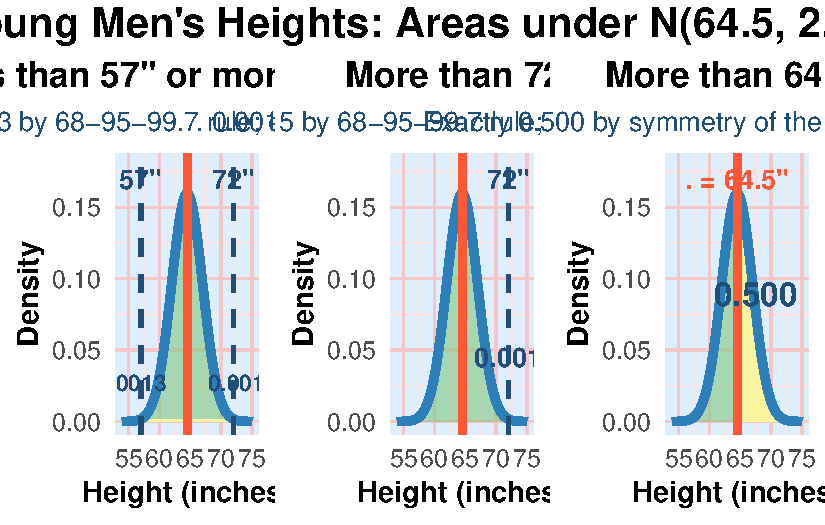
\includegraphics[keepaspectratio]{index_files/figure-pdf/unnamed-chunk-28-1.pdf}}

\section{Normal model for young women's
heights}\label{normal-model-for-young-womens-heights}

In the graph above, young women's heights are well approximated by a
normal distribution with mean \textbf{mu = 64.5 inches} (about 5 feet
4.5 inches) and standard deviation \textbf{sigma = 2.5 inches}. The
normal curve is bell-shaped and symmetric: the mean equals the median,
and the distribution is centered at mu. The points of inflection (where
the curve changes concavity) occur at \textbf{mu +/- sigma}. These
locations provide a visual guide to one standard deviation from the
center. In this book we denote the model by \textbf{N(64.5, 2.5)},
meaning ``normal with mean 64.5 and standard deviation 2.5.'' (Some
sources use N(mu, sigma\^{}2); here we use N(mu, sigma).)

\section{Interpreting mu and sigma}\label{interpreting-mu-and-sigma}

\begin{itemize}
\tightlist
\item
  \textbf{mu (location)}: moves the curve left or right; it is the
  center of the distribution and equals the typical value for a
  symmetric normal.\\
\item
  \textbf{sigma (scale)}: controls spread; larger sigma makes the curve
  flatter and wider, smaller sigma makes it taller and narrower.\\
\item
  \textbf{Units}: mu and sigma are in the same units as the data
  (inches). Conversions to feet/inches are for interpretation only.
\end{itemize}

\subsection{The 68--95--99.7 rule (empirical
rule)}\label{the-689599.7-rule-empirical-rule}

For any normal distribution: - About \textbf{68\%} of observations lie
within \textbf{mu +/- 1\emph{sigma\textbf{. - About }95\%\textbf{ lie
within }mu +/- 2}sigma}. - About \textbf{99.7\%} lie within **mu +/-
3*sigma**.

Applied to \textbf{N(64.5, 2.5)}: - \textbf{{[}62.0, 67.0{]}} (64.5 +/-
2.5) contains about \textbf{68\%}. - \textbf{{[}59.5, 69.5{]}} (64.5 +/-
5.0) contains about \textbf{95\%}. - \textbf{{[}57.0, 72.0{]}} (64.5 +/-
7.5) contains about \textbf{99.7\%}.

\emph{Rule-of-thumb vs exact}: The empirical rule is quick and close.
Exact central 95\% uses **mu +/- 1.96*sigma** (not exactly 2*sigma).
Software or a standard normal table gives exact areas.

\section{Standardization (z-scores)}\label{standardization-z-scores}

To place any value x on the standard normal scale, compute \textbf{z =
(x − mu) / sigma}.\\
- z counts how many standard deviations x is from the mean.\\
- Areas such as P(X \textless= x) become P(Z \textless= z) on the
standard normal, which can be looked up or computed with software.

For \textbf{N(64.5, 2.5)}: - x = 72 -\textgreater{} z = (72 − 64.5)/2.5
= \textbf{+3.0}\\
- x = 57 -\textgreater{} z = (57 − 64.5)/2.5 = \textbf{−3.0}

\section{questions}\label{questions}

\textbf{1) Percent shorter than 57 inches or taller than 72 inches.}\\
- Sketch the normal curve, mark mu = 64.5 and the cutoffs 57 and 72.
Shade both tails.

\begin{itemize}
\item
  Recognize that 57 = mu − 3\emph{sigma and 72 = mu + 3}sigma.\\
\item
  By the empirical rule, the total area outside **mu +/- 3*sigma\textbf{
  is about }0.003** (0.3\%).
\item
  By symmetry, each tail is about \textbf{0.0015} (0.15\%).\\
\item
  (Exact reference: two-sided area at \textbar z\textbar{} \textgreater=
  3 is \textasciitilde0.0027, so each tail \textasciitilde0.00135.)
\end{itemize}

\textbf{2) Percent taller than 72 inches.}\\
- This is the right tail beyond mu + 3*sigma.\\
- Empirical rule: approximately \textbf{0.0015} (0.15\%).\\
- (Exact: \textasciitilde0.00135.)

\textbf{3) Percent taller than 64.5 inches.}\\
- 64.5 is the mean (and median) of a symmetric normal.\\
- Exactly \textbf{0.500} (50\%) of the distribution lies above mu.\\
- Interpretation: roughly half of young women are taller than 64.5
inches and half are shorter.

\section{How to solve normal-probability problems
(checklist)}\label{how-to-solve-normal-probability-problems-checklist}

\begin{enumerate}
\def\labelenumi{\arabic{enumi})}
\tightlist
\item
  \textbf{Draw and label} the curve with mu and the relevant cut
  points.\\
\item
  \textbf{Shade} the region that matches the probability statement.\\
\item
  \textbf{Standardize} each numerical boundary: z = (x − mu)/sigma.\\
\item
  \textbf{Find area}: use the empirical rule for quick estimates; use
  software/tables for exact values.\\
\item
  \textbf{Sanity-check} against the sketch (tiny region -\textgreater{}
  small probability; half-curve -\textgreater{} \textasciitilde0.5).\\
\item
  \textbf{Report clearly} in proportion or percent and interpret in
  context (with units).
\end{enumerate}

\bookmarksetup{startatroot}

\chapter{Chapter 4:Scatterplots and
Correlations}\label{chapter-4scatterplots-and-correlations}

Up to now we have focused on one variable at a time (univariate
analysis): distributions of outcomes like income or test scores and how
to describe their shape. Many questions in the social sciences, however,
ask how two quantitative variables move together---for example, whether
places with higher inequality also report lower support for
redistribution, or whether graduate-education rates are associated with
voter turnout. This section introduces scatter plots and correlation for
such bivariate analysis.

\section{Explanatory vs.~Response
Variables}\label{explanatory-vs.-response-variables}

When studying a pair of variables, it helps to state which one is
treated as explanatory (often called the independent variable) and which
is the response (dependent variable). The explanatory variable is the
putative ``input'' you think may help account for variation in the
response. Declaring roles does not prove causality; it simply clarifies
your research hypothesis and how you will present the graph. Convention:
put the explanatory variable on the x-axis and the response variable on
the y-axis.

\#\#Reading a Scatter Plot

When you examine a scatter plot, look for four things: Form: linear,
curved, clustered, or no visible structure. Direction: positive
(upward), negative (downward), or none. Strength: how tightly points
track the pattern (strong vs.~weak). Deviations: unusual points
(outliers) that don't fit the overall pattern. A point can be an outlier
without being extreme on x or y individually; it can be unusual relative
to the relationship.

Example A (political behavior): Graduate education \& voter turnout
Hypothesis: counties with a larger share of residents holding graduate
degrees tend to exhibit higher general-election turnout.

\begin{Shaded}
\begin{Highlighting}[]
\FunctionTok{set.seed}\NormalTok{(}\DecValTok{42}\NormalTok{)}
\FunctionTok{library}\NormalTok{(dplyr)}
\FunctionTok{library}\NormalTok{(ggplot2)}

\NormalTok{n }\OtherTok{\textless{}{-}} \DecValTok{600}
\NormalTok{dat\_turnout }\OtherTok{\textless{}{-}} \FunctionTok{tibble}\NormalTok{(}
  \AttributeTok{county =} \FunctionTok{paste0}\NormalTok{(}\StringTok{"C"}\NormalTok{, }\FunctionTok{seq\_len}\NormalTok{(n)),}
  \AttributeTok{grad\_share =} \FunctionTok{pmin}\NormalTok{(}\FunctionTok{pmax}\NormalTok{(}\FunctionTok{rbeta}\NormalTok{(n, }\DecValTok{2}\NormalTok{, }\DecValTok{6}\NormalTok{)}\SpecialCharTok{*}\FloatTok{0.45}\NormalTok{, }\FloatTok{0.005}\NormalTok{), }\FloatTok{0.45}\NormalTok{), }\CommentTok{\# 0–45\%}
  \AttributeTok{turnout =} \DecValTok{40} \SpecialCharTok{+} \DecValTok{55}\SpecialCharTok{*}\NormalTok{grad\_share }\SpecialCharTok{+} \FunctionTok{rnorm}\NormalTok{(n, }\DecValTok{0}\NormalTok{, }\DecValTok{5}\NormalTok{)              }\CommentTok{\# \%}
\NormalTok{) }\SpecialCharTok{|\textgreater{}}
  \FunctionTok{mutate}\NormalTok{(}\AttributeTok{turnout =} \FunctionTok{pmin}\NormalTok{(}\FunctionTok{pmax}\NormalTok{(turnout, }\DecValTok{25}\NormalTok{), }\DecValTok{85}\NormalTok{))}


\FunctionTok{ggplot}\NormalTok{(dat\_turnout, }\FunctionTok{aes}\NormalTok{(grad\_share }\SpecialCharTok{*} \DecValTok{100}\NormalTok{, turnout)) }\SpecialCharTok{+}
  \FunctionTok{geom\_point}\NormalTok{(}\AttributeTok{alpha =} \FloatTok{0.4}\NormalTok{, }\AttributeTok{size =} \DecValTok{3}\NormalTok{, }\AttributeTok{colour =} \StringTok{"red"}\NormalTok{) }\SpecialCharTok{+}
  \FunctionTok{geom\_smooth}\NormalTok{(}\AttributeTok{method =} \StringTok{"lm"}\NormalTok{, }\AttributeTok{se =} \ConstantTok{TRUE}\NormalTok{) }\SpecialCharTok{+}
  \FunctionTok{labs}\NormalTok{(}
    \AttributeTok{x =} \StringTok{"Graduate{-}degree share (\%)"}\NormalTok{,}
    \AttributeTok{y =} \StringTok{"General{-}election turnout (\%)"}\NormalTok{,}
    \AttributeTok{title =} \StringTok{"More graduate education, higher turnout (illustrative)"}
\NormalTok{  ) }\SpecialCharTok{+}
  \FunctionTok{theme}\NormalTok{(}
    \AttributeTok{plot.title =} \FunctionTok{element\_text}\NormalTok{(}\AttributeTok{size =} \DecValTok{20}\NormalTok{, }\AttributeTok{face =} \StringTok{"bold"}\NormalTok{),}
    \AttributeTok{axis.title =} \FunctionTok{element\_text}\NormalTok{(}\AttributeTok{size =} \DecValTok{16}\NormalTok{),}
    \AttributeTok{axis.text =} \FunctionTok{element\_text}\NormalTok{(}\AttributeTok{size =} \DecValTok{14}\NormalTok{)}
\NormalTok{  )  }\SpecialCharTok{+} \FunctionTok{theme\_classic}\NormalTok{()}


\CommentTok{\#| label: cor{-}grad{-}turnout}
\CommentTok{\#| echo: true}
\FunctionTok{cor}\NormalTok{(dat\_turnout}\SpecialCharTok{$}\NormalTok{grad\_share, dat\_turnout}\SpecialCharTok{$}\NormalTok{turnout)  }\CommentTok{\# Pearson correlation}
\end{Highlighting}
\end{Shaded}

\begin{verbatim}
[1] 0.604028
\end{verbatim}

\begin{figure}[H]

\centering{

\pandocbounded{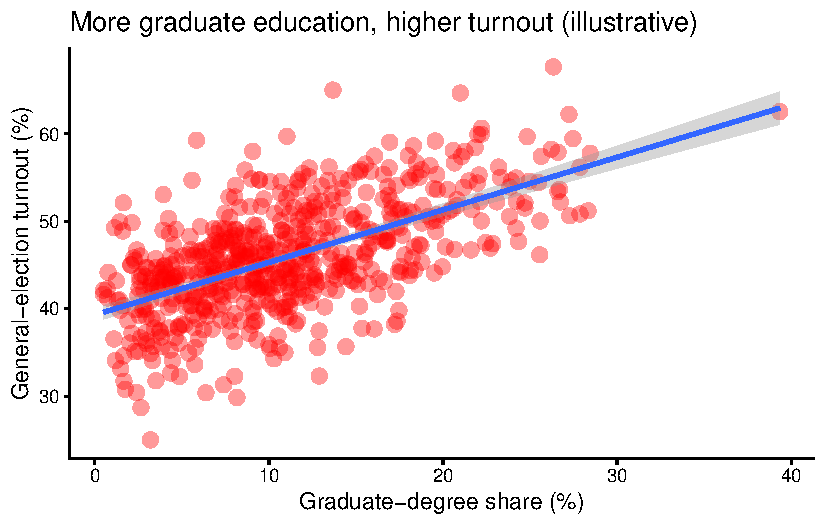
\includegraphics[keepaspectratio]{index_files/figure-pdf/fig-grad-turnout-1.pdf}}

}

\caption{\label{fig-grad-turnout}County-level relationship between
graduate-degree share and voter turnout (synthetic illustration).}

\end{figure}%

The scatterplot illustrating the relationship between graduate-degree
share and voter turnout depicts a strong, positive linear association.
Each point represents a county, and the overall configuration of the
points aligns closely with the upward-sloping regression line. Counties
with a larger proportion of residents holding graduate degrees tend to
exhibit higher rates of electoral participation. The linearity of the
pattern suggests that this relationship can be well-approximated by a
straight line, implying that each incremental increase in graduate
education corresponds to a roughly proportional increase in turnout. The
dispersion of points around the fitted line is moderate, indicating that
while the general trend holds across most counties, local
variation---possibly due to institutional factors such as registration
laws or political mobilization---still exists. There are few, if any,
extreme outliers, which implies that the association is broadly
consistent across the sample. Interpretation: points trend upward
(positive direction) with a fairly linear form; the regression line
helps visualize the direction and strength. The correlation summarizes
the linear association numerically.

Example B: Inequality \& support for redistribution Hypothesis: higher
income inequality (Gini coefficient) is associated with greater support
for redistribution in cross-national survey aggregates.

\begin{Shaded}
\begin{Highlighting}[]
\CommentTok{\#| label: fig{-}gini{-}redis}
\CommentTok{\#| fig{-}cap: "Cross{-}national inequality vs. redistribution support (synthetic). OLS fit with 95\% CI."}
\CommentTok{\#| fig{-}width: 7.5}
\CommentTok{\#| fig{-}height: 5}
\CommentTok{\#| dpi: 320}
\CommentTok{\#| warning: false}
\CommentTok{\#| message: false}

\FunctionTok{set.seed}\NormalTok{(}\DecValTok{7}\NormalTok{)}
\FunctionTok{library}\NormalTok{(dplyr)}
\FunctionTok{library}\NormalTok{(ggplot2)}
\FunctionTok{library}\NormalTok{(scales)}

\NormalTok{n }\OtherTok{\textless{}{-}} \DecValTok{45}
\NormalTok{dat\_redis }\OtherTok{\textless{}{-}} \FunctionTok{tibble}\NormalTok{(}
  \AttributeTok{country =} \FunctionTok{paste0}\NormalTok{(}\StringTok{"Country\_"}\NormalTok{, }\FunctionTok{seq\_len}\NormalTok{(n)),}
  \AttributeTok{gini =} \FunctionTok{runif}\NormalTok{(n, }\FloatTok{0.24}\NormalTok{, }\FloatTok{0.52}\NormalTok{),}
  \AttributeTok{support\_redis =} \DecValTok{20} \SpecialCharTok{+} \DecValTok{120}\SpecialCharTok{*}\NormalTok{(gini }\SpecialCharTok{{-}} \FunctionTok{min}\NormalTok{(gini)) }\SpecialCharTok{+} \FunctionTok{rnorm}\NormalTok{(n, }\DecValTok{0}\NormalTok{, }\DecValTok{10}\NormalTok{)}
\NormalTok{) }\SpecialCharTok{|\textgreater{}}
  \FunctionTok{mutate}\NormalTok{(}\AttributeTok{support\_redis =} \FunctionTok{pmin}\NormalTok{(}\FunctionTok{pmax}\NormalTok{(support\_redis, }\DecValTok{10}\NormalTok{), }\DecValTok{95}\NormalTok{))}

\NormalTok{outlier }\OtherTok{\textless{}{-}} \FunctionTok{tibble}\NormalTok{(}\AttributeTok{country =} \StringTok{"Outlierland"}\NormalTok{, }\AttributeTok{gini =} \FloatTok{0.50}\NormalTok{, }\AttributeTok{support\_redis =} \DecValTok{25}\NormalTok{)}
\NormalTok{dat\_redis2 }\OtherTok{\textless{}{-}} \FunctionTok{bind\_rows}\NormalTok{(dat\_redis, outlier)}

\NormalTok{theme\_pnas }\OtherTok{\textless{}{-}} \ControlFlowTok{function}\NormalTok{(}\AttributeTok{base\_size =} \DecValTok{15}\NormalTok{)\{}
  \FunctionTok{theme\_minimal}\NormalTok{(}\AttributeTok{base\_size =}\NormalTok{ base\_size) }\SpecialCharTok{+}
    \FunctionTok{theme}\NormalTok{(}
      \AttributeTok{text =} \FunctionTok{element\_text}\NormalTok{(}\AttributeTok{color =} \StringTok{"\#222222"}\NormalTok{),}
      \AttributeTok{plot.title =} \FunctionTok{element\_text}\NormalTok{(}\AttributeTok{size =}\NormalTok{ base\_size }\SpecialCharTok{+} \DecValTok{7}\NormalTok{, }\AttributeTok{face =} \StringTok{"bold"}\NormalTok{, }\AttributeTok{hjust =} \DecValTok{0}\NormalTok{),}
      \AttributeTok{plot.subtitle =} \FunctionTok{element\_text}\NormalTok{(}\AttributeTok{size =}\NormalTok{ base\_size }\SpecialCharTok{+} \DecValTok{1}\NormalTok{, }\AttributeTok{margin =} \FunctionTok{margin}\NormalTok{(}\AttributeTok{b =} \DecValTok{6}\NormalTok{)),}
      \AttributeTok{plot.caption =} \FunctionTok{element\_text}\NormalTok{(}\AttributeTok{size =}\NormalTok{ base\_size }\SpecialCharTok{{-}} \DecValTok{2}\NormalTok{, }\AttributeTok{color =} \StringTok{"\#666666"}\NormalTok{),}
      \AttributeTok{axis.title =} \FunctionTok{element\_text}\NormalTok{(}\AttributeTok{size =}\NormalTok{ base\_size }\SpecialCharTok{+} \DecValTok{3}\NormalTok{, }\AttributeTok{face =} \StringTok{"bold"}\NormalTok{),}
      \AttributeTok{axis.text =} \FunctionTok{element\_text}\NormalTok{(}\AttributeTok{size =}\NormalTok{ base\_size),}
      \AttributeTok{panel.grid.major =} \FunctionTok{element\_line}\NormalTok{(}\AttributeTok{color =} \StringTok{"\#e6e6e6"}\NormalTok{, }\AttributeTok{linewidth =} \FloatTok{0.6}\NormalTok{),}
      \AttributeTok{panel.grid.minor =} \FunctionTok{element\_blank}\NormalTok{(),}
      \AttributeTok{axis.line =} \FunctionTok{element\_line}\NormalTok{(}\AttributeTok{color =} \StringTok{"\#222222"}\NormalTok{, }\AttributeTok{linewidth =} \FloatTok{0.6}\NormalTok{),}
      \AttributeTok{plot.margin =} \FunctionTok{margin}\NormalTok{(}\DecValTok{8}\NormalTok{, }\DecValTok{14}\NormalTok{, }\DecValTok{8}\NormalTok{, }\DecValTok{8}\NormalTok{)}
\NormalTok{    )}
\NormalTok{\}}

\NormalTok{col\_point\_fill }\OtherTok{\textless{}{-}} \StringTok{"\#D32F2F"}  \CommentTok{\# red fill}
\NormalTok{col\_point\_edge }\OtherTok{\textless{}{-}} \StringTok{"\#8E0000"}  \CommentTok{\# darker red stroke}
\NormalTok{col\_line       }\OtherTok{\textless{}{-}} \StringTok{"\#1565C0"}  \CommentTok{\# fit line}
\NormalTok{col\_rug        }\OtherTok{\textless{}{-}} \StringTok{"\#bdbdbd"}  \CommentTok{\# subtle rugs}

\FunctionTok{ggplot}\NormalTok{(dat\_redis2, }\FunctionTok{aes}\NormalTok{(gini, support\_redis)) }\SpecialCharTok{+}
  \FunctionTok{geom\_rug}\NormalTok{(}\AttributeTok{sides =} \StringTok{"b"}\NormalTok{, }\AttributeTok{alpha =} \FloatTok{0.35}\NormalTok{, }\AttributeTok{color =}\NormalTok{ col\_rug, }\AttributeTok{linewidth =} \FloatTok{0.4}\NormalTok{) }\SpecialCharTok{+}
  \FunctionTok{geom\_rug}\NormalTok{(}\AttributeTok{sides =} \StringTok{"l"}\NormalTok{, }\AttributeTok{alpha =} \FloatTok{0.35}\NormalTok{, }\AttributeTok{color =}\NormalTok{ col\_rug, }\AttributeTok{linewidth =} \FloatTok{0.4}\NormalTok{) }\SpecialCharTok{+}
  \FunctionTok{geom\_point}\NormalTok{(}\AttributeTok{shape =} \DecValTok{21}\NormalTok{, }\AttributeTok{size =} \DecValTok{2}\NormalTok{, }\AttributeTok{stroke =} \FloatTok{0.7}\NormalTok{,}
             \AttributeTok{color =}\NormalTok{ col\_point\_edge, }\AttributeTok{fill =} \FunctionTok{alpha}\NormalTok{(col\_point\_fill, }\FloatTok{0.85}\NormalTok{)) }\SpecialCharTok{+}
  \FunctionTok{geom\_smooth}\NormalTok{(}\AttributeTok{method =} \StringTok{"lm"}\NormalTok{, }\AttributeTok{se =} \ConstantTok{TRUE}\NormalTok{, }\AttributeTok{color =}\NormalTok{ col\_line,}
              \AttributeTok{fill =} \FunctionTok{alpha}\NormalTok{(col\_line, }\FloatTok{0.12}\NormalTok{), }\AttributeTok{linewidth =} \FloatTok{1.2}\NormalTok{) }\SpecialCharTok{+}
  \FunctionTok{labs}\NormalTok{(}
    \AttributeTok{x =} \StringTok{"Gini coefficient (income inequality)"}\NormalTok{,}
    \AttributeTok{y =} \StringTok{"Support for redistribution (\%)"}\NormalTok{,}
    \AttributeTok{title =} \StringTok{"Greater inequality aligns with higher demand for redistribution"}\NormalTok{,}
    \AttributeTok{subtitle =} \StringTok{"OLS fit with 95\% confidence band"}\NormalTok{,}
    \AttributeTok{caption =} \StringTok{"Synthetic data for illustration"}
\NormalTok{  ) }\SpecialCharTok{+}
  \FunctionTok{scale\_x\_continuous}\NormalTok{(}
    \AttributeTok{limits =} \FunctionTok{c}\NormalTok{(}\FloatTok{0.24}\NormalTok{, }\FloatTok{0.52}\NormalTok{),}
    \AttributeTok{breaks =} \FunctionTok{seq}\NormalTok{(}\FloatTok{0.24}\NormalTok{, }\FloatTok{0.52}\NormalTok{, }\AttributeTok{by =} \FloatTok{0.04}\NormalTok{),}
    \AttributeTok{labels =} \FunctionTok{number\_format}\NormalTok{(}\AttributeTok{accuracy =} \FloatTok{0.01}\NormalTok{),}
    \AttributeTok{expand =} \FunctionTok{expansion}\NormalTok{(}\AttributeTok{mult =} \FunctionTok{c}\NormalTok{(}\FloatTok{0.015}\NormalTok{, }\FloatTok{0.03}\NormalTok{))}
\NormalTok{  ) }\SpecialCharTok{+}
  \FunctionTok{scale\_y\_continuous}\NormalTok{(}
    \AttributeTok{limits =} \FunctionTok{c}\NormalTok{(}\DecValTok{10}\NormalTok{, }\DecValTok{95}\NormalTok{),}
    \AttributeTok{breaks =} \FunctionTok{seq}\NormalTok{(}\DecValTok{10}\NormalTok{, }\DecValTok{90}\NormalTok{, }\AttributeTok{by =} \DecValTok{10}\NormalTok{),}
    \AttributeTok{expand =} \FunctionTok{expansion}\NormalTok{(}\AttributeTok{mult =} \FunctionTok{c}\NormalTok{(}\FloatTok{0.02}\NormalTok{, }\FloatTok{0.04}\NormalTok{))}
\NormalTok{  ) }\SpecialCharTok{+}
  \FunctionTok{theme\_pnas}\NormalTok{()}
\end{Highlighting}
\end{Shaded}

\pandocbounded{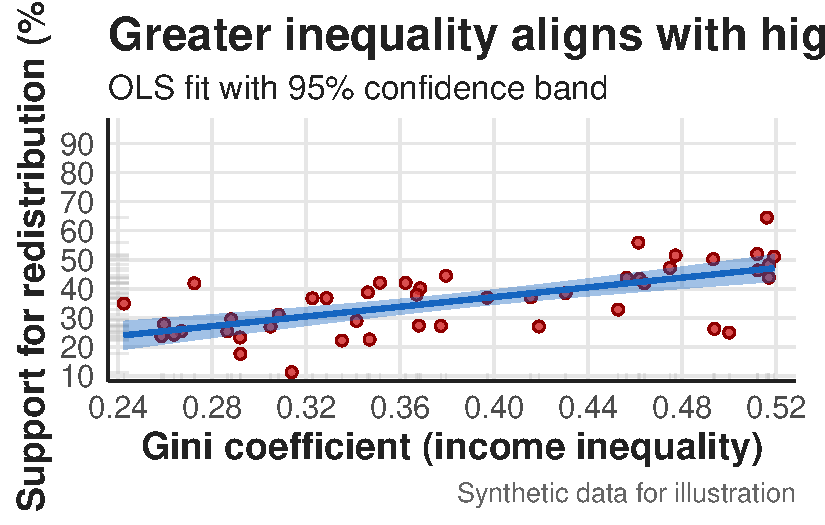
\includegraphics[keepaspectratio]{index_files/figure-pdf/unnamed-chunk-29-1.pdf}}

\begin{Shaded}
\begin{Highlighting}[]
\CommentTok{\#| label: cor{-}gini{-}redis}
\FunctionTok{cor}\NormalTok{(dat\_redis2}\SpecialCharTok{$}\NormalTok{gini, dat\_redis2}\SpecialCharTok{$}\NormalTok{support\_redis)}
\end{Highlighting}
\end{Shaded}

\begin{verbatim}
[1] 0.657166
\end{verbatim}

The cross-national scatterplot relating the Gini coefficient to support
for redistribution reveals a more complex pattern. The main cluster of
observations follows a moderate positive trend, suggesting that citizens
in more unequal societies express somewhat stronger support for
redistributive policies. However, the relationship is less tightly
clustered than in the turnout example, implying weaker predictive power
and the influence of contextual moderators---such as partisan
competition, media framing, or welfare-state legacies. A notable
outlier, labeled Outlierland, exhibits an unusually high Gini
coefficient but comparatively low redistributive support. This case
exerts visible leverage on the regression line, flattening the slope and
reducing the estimated correlation. Its presence highlights the
importance of substantive diagnosis: rather than dismissing it as a
statistical anomaly, researchers should ask whether this country's
political economy---perhaps resource dependence or clientelistic
governance---represents a distinct mechanism. When the outlier is
removed, the fitted line steepens considerably, illustrating how
influential observations can reshape both visual and statistical
summaries.

Outliers can mask patterns. If the outlier reflects a different
data-generating process (e.g., unusually high commodity rents and weak
party system linkages), you might show results with and without it:

\begin{Shaded}
\begin{Highlighting}[]
\FunctionTok{library}\NormalTok{(broom)}
\NormalTok{m\_all }\OtherTok{\textless{}{-}} \FunctionTok{lm}\NormalTok{(support\_redis }\SpecialCharTok{\textasciitilde{}}\NormalTok{ gini, dat\_redis2)}
\NormalTok{m\_no\_out }\OtherTok{\textless{}{-}} \FunctionTok{lm}\NormalTok{(support\_redis }\SpecialCharTok{\textasciitilde{}}\NormalTok{ gini, }\FunctionTok{filter}\NormalTok{(dat\_redis2, country }\SpecialCharTok{!=} \StringTok{"Outlierland"}\NormalTok{))}

\FunctionTok{bind\_rows}\NormalTok{(}
  \FunctionTok{tidy}\NormalTok{(m\_all) }\SpecialCharTok{|\textgreater{}} \FunctionTok{mutate}\NormalTok{(}\AttributeTok{model =} \StringTok{"All cases"}\NormalTok{),}
  \FunctionTok{tidy}\NormalTok{(m\_no\_out) }\SpecialCharTok{|\textgreater{}} \FunctionTok{mutate}\NormalTok{(}\AttributeTok{model =} \StringTok{"Excluding outlier"}\NormalTok{)}
\NormalTok{)}
\end{Highlighting}
\end{Shaded}

\begin{verbatim}
# A tibble: 4 x 6
  term        estimate std.error statistic      p.value model            
  <chr>          <dbl>     <dbl>     <dbl>        <dbl> <chr>            
1 (Intercept)     3.87      5.69     0.679 0.500        All cases        
2 gini           83.3      14.4      5.78  0.000000702  All cases        
3 (Intercept)     1.61      5.41     0.297 0.768        Excluding outlier
4 gini           90.4      13.8      6.56  0.0000000561 Excluding outlier
\end{verbatim}

\begin{Shaded}
\begin{Highlighting}[]
\CommentTok{\#| label: fig{-}edu{-}vax}
\CommentTok{\#| fig{-}cap: "State education and vaccination rates."}

\FunctionTok{set.seed}\NormalTok{(}\DecValTok{123}\NormalTok{)}
\NormalTok{states }\OtherTok{\textless{}{-}}\NormalTok{ state.abb[}\DecValTok{1}\SpecialCharTok{:}\DecValTok{48}\NormalTok{] }\CommentTok{\# use 48 for a clean grid}
\NormalTok{dat\_vax }\OtherTok{\textless{}{-}} \FunctionTok{tibble}\NormalTok{(}
  \AttributeTok{state =}\NormalTok{ states,}
  \AttributeTok{college =} \FunctionTok{runif}\NormalTok{(}\FunctionTok{length}\NormalTok{(states), }\FloatTok{0.18}\NormalTok{, }\FloatTok{0.48}\NormalTok{),  }\CommentTok{\# share BA+}
  \AttributeTok{vax\_rate =} \DecValTok{45} \SpecialCharTok{+} \DecValTok{80}\SpecialCharTok{*}\NormalTok{college }\SpecialCharTok{+} \FunctionTok{rnorm}\NormalTok{(}\FunctionTok{length}\NormalTok{(states), }\DecValTok{0}\NormalTok{, }\DecValTok{6}\NormalTok{)}
\NormalTok{) }\SpecialCharTok{|\textgreater{}}
  \FunctionTok{mutate}\NormalTok{(}\AttributeTok{vax\_rate =} \FunctionTok{pmin}\NormalTok{(}\FunctionTok{pmax}\NormalTok{(vax\_rate, }\DecValTok{35}\NormalTok{), }\DecValTok{95}\NormalTok{))}

\FunctionTok{ggplot}\NormalTok{(dat\_vax, }\FunctionTok{aes}\NormalTok{(college}\SpecialCharTok{*}\DecValTok{100}\NormalTok{, vax\_rate, }\AttributeTok{label =}\NormalTok{ state)) }\SpecialCharTok{+}
  \FunctionTok{geom\_point}\NormalTok{(}\AttributeTok{colour =} \StringTok{"violet"}\NormalTok{, }\AttributeTok{size =} \DecValTok{3}\NormalTok{) }\SpecialCharTok{+}
  \FunctionTok{geom\_smooth}\NormalTok{(}\AttributeTok{method =} \StringTok{"lm"}\NormalTok{, }\AttributeTok{se =} \ConstantTok{TRUE}\NormalTok{) }\SpecialCharTok{+}
\NormalTok{  ggrepel}\SpecialCharTok{::}\FunctionTok{geom\_text\_repel}\NormalTok{(}\AttributeTok{size =} \DecValTok{7}\NormalTok{) }\SpecialCharTok{+}
  \FunctionTok{labs}\NormalTok{(}
    \AttributeTok{x =} \StringTok{"College completion (\%)"}\NormalTok{,}
    \AttributeTok{y =} \StringTok{"Adult vaccination rate (\%)"}\NormalTok{,}
    \AttributeTok{title =} \StringTok{"Education is positively associated with vaccination"}
\NormalTok{  ) }\SpecialCharTok{+}
  \FunctionTok{theme}\NormalTok{(}
    \AttributeTok{axis.text  =} \FunctionTok{element\_text}\NormalTok{(}\AttributeTok{size =} \DecValTok{16}\NormalTok{),                     }\CommentTok{\# tick labels}
    \AttributeTok{axis.title.x =} \FunctionTok{element\_text}\NormalTok{(}\AttributeTok{size =} \DecValTok{22}\NormalTok{, }\AttributeTok{face =} \StringTok{"bold"}\NormalTok{, }
                                 \AttributeTok{margin =} \FunctionTok{margin}\NormalTok{(}\AttributeTok{t =} \DecValTok{10}\NormalTok{)),}
    \AttributeTok{axis.title.y =} \FunctionTok{element\_text}\NormalTok{(}\AttributeTok{size =} \DecValTok{22}\NormalTok{, }\AttributeTok{face =} \StringTok{"bold"}\NormalTok{, }
                                 \AttributeTok{margin =} \FunctionTok{margin}\NormalTok{(}\AttributeTok{r =} \DecValTok{10}\NormalTok{)),}
    \AttributeTok{plot.title =} \FunctionTok{element\_text}\NormalTok{(}\AttributeTok{size =} \DecValTok{24}\NormalTok{, }\AttributeTok{face =} \StringTok{"bold"}\NormalTok{)}
\NormalTok{  )}
\end{Highlighting}
\end{Shaded}

\pandocbounded{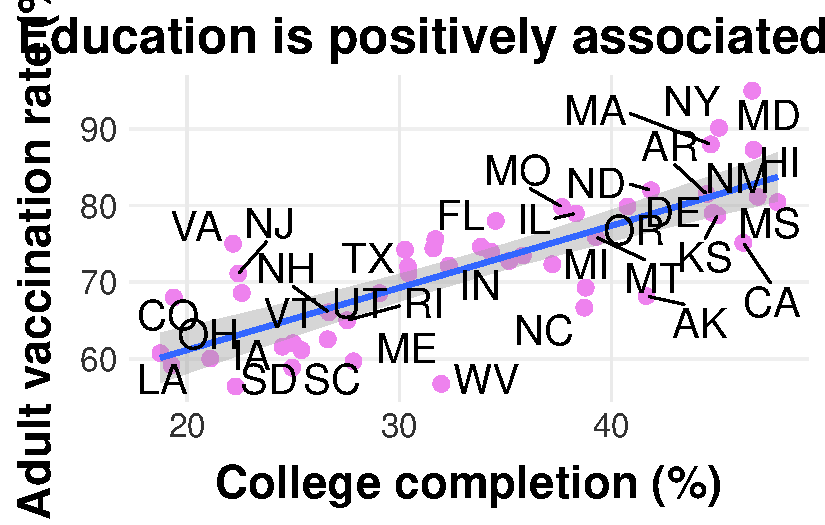
\includegraphics[keepaspectratio]{index_files/figure-pdf/unnamed-chunk-30-1.pdf}}

\begin{Shaded}
\begin{Highlighting}[]
\CommentTok{\#| label: cor{-}edu{-}vax}
\FunctionTok{c}\NormalTok{(}\AttributeTok{Pearson =} \FunctionTok{cor}\NormalTok{(dat\_vax}\SpecialCharTok{$}\NormalTok{college, dat\_vax}\SpecialCharTok{$}\NormalTok{vax\_rate),}
  \AttributeTok{Spearman =} \FunctionTok{cor}\NormalTok{(dat\_vax}\SpecialCharTok{$}\NormalTok{college, dat\_vax}\SpecialCharTok{$}\NormalTok{vax\_rate, }\AttributeTok{method =} \StringTok{"spearman"}\NormalTok{))}
\end{Highlighting}
\end{Shaded}

\begin{verbatim}
  Pearson  Spearman 
0.7865221 0.7964611 
\end{verbatim}

The state-level scatterplot linking college completion rates to adult
vaccination displays a robust, positive, and nearly linear relationship.
States with higher proportions of college-educated residents tend to
have substantially greater vaccination coverage. The slope of the fitted
line is steep, and the residual spread around it is relatively small,
denoting a strong correlation. The linear fit captures the pattern well;
no evident curvature suggests non-linearity. A few states deviate
modestly above or below the line---these may correspond to cases where
political polarization or health-infrastructure disparities mediate the
education-vaccination link---but none appear to qualify as statistical
outliers. The correlation coefficients reinforce this visual impression:
both the Pearson (linear) and Spearman (rank-based) measures are high
and positive, confirming that the association holds in both magnitude
and rank order. Substantively, the scatterplot provides an intuitive
demonstration of how social stratification, measured through educational
attainment, aligns with patterns of compliance and trust in science
across political contexts.

\section{Pearson vs.~Spearman}\label{pearson-vs.-spearman}

Pearson quantifies linear association; Spearman correlates ranks and is
robust to monotone but non-linear relationships.

\emph{Cross-Plot Comparison and Interpretation} Viewed together, these
scatterplots illustrate key principles of quantitative reasoning in the
social sciences. The form of association ranges from strongly linear
(education--turnout, education--vaccination) to modestly linear with
influential cases (inequality--redistribution). The direction is
uniformly positive, consistent with theories that link human capital or
economic inequality to civic and policy attitudes. The strength varies:
correlations exceeding 0.7 denote tight coupling, whereas values around
0.4--0.5 imply more diffuse relationships shaped by intervening
variables. Finally, outliers---whether individual counties or
countries---remind us that statistical associations must always be
interpreted through substantive context, not treated as mechanical
regularities.

These formal interpretations serve as models for how sociologists and
political scientists should describe scatterplots in analytical writing:
discuss direction, form, strength, outliers, and the plausible social
mechanisms underlying each observed pattern.

\subsection{Scatterplots, Grouping by a Third Variable, and the
Correlation
Coefficient}\label{scatterplots-grouping-by-a-third-variable-and-the-correlation-coefficient}

A scatterplot displays how two quantitative variables vary together. In
comparative social science, however, relationships often differ across
types of cases (e.g., established versus newer democracies; union-dense
versus union-sparse polities). When a third variable meaningfully
partitions the sample, the right approach is not one big cloud but two
(or more) overlaid clouds---each with its own pattern. For instance, the
association between social trust (horizontal axis) and general-election
turnout (vertical axis) may be positive in both established and newer
democracies, yet the slope and elevation can differ: established
democracies might cluster at higher turnout for any given trust level.
The plot should make that visible with distinct aesthetics (color/shape)
and, ideally, a separate fitted line per group. In other words, the
figure contains multiple scatterplots at once---one for each
category---so readers can judge whether the relationship is common
across groups or appears group-specific.

When describing such plots formally, report: (i) direction (positive,
negative, none); (ii) form (roughly linear, curved, clustered,
segmented); (iii) strength (tight vs.~diffuse cloud around the trend);
and (iv) deviations (outliers or leverage points). If groups trace
parallel lines, a common mechanism with group-specific intercepts is
plausible; if slopes differ, the third variable likely moderates the
relationship. Avoid merging unlike groups into a single fit that
obscures heterogeneity---doing so invites misleading summaries and
errors in inference.

\subsection{What is a correlation
coefficient?}\label{what-is-a-correlation-coefficient}

The correlation coefficient (Pearson's r) is a unit-free index
summarizing the direction and strength of a linear relationship between
two quantitative variables. Values range from −1 (perfect decreasing
linear relation) to +1 (perfect increasing linear relation), with 0
indicating no linear association. Because r is computed from
standardized values (subtract the mean and divide by the standard
deviation for each variable), it is invariant to changes in units (e.g.,
dollars vs.~thousands of dollars) and symmetric in x and y (swapping
axes does not change r). Crucially, correlation is not resistant to
outliers: a single unusual case can meaningfully inflate or attenuate r.
And correlation does not establish causation; it merely quantifies
co-movement conditional on linear form.

Use r only when the pattern is plausibly linear and both variables are
quantitative. For categorical variables, or when the ordering of
categories is arbitrary, precision language is ``association,'' not
``correlation.'' If curvature is evident, consider transformations or
non-linear modeling; a single number like Pearson's r will misrepresent
the underlying relationship. Finally, when outliers exist, present
results with and without them and explain, substantively, what makes
those cases different.

\begin{Shaded}
\begin{Highlighting}[]
\FunctionTok{set.seed}\NormalTok{(}\DecValTok{101}\NormalTok{)}
\FunctionTok{library}\NormalTok{(dplyr)}
\FunctionTok{library}\NormalTok{(ggplot2)}
\FunctionTok{library}\NormalTok{(scales)}

\CommentTok{\# Synthetic comparative dataset}
\NormalTok{n }\OtherTok{\textless{}{-}} \DecValTok{200}
\NormalTok{dat\_trust }\OtherTok{\textless{}{-}} \FunctionTok{tibble}\NormalTok{(}
  \AttributeTok{regime =} \FunctionTok{sample}\NormalTok{(}\FunctionTok{c}\NormalTok{(}\StringTok{"Established democracy"}\NormalTok{, }\StringTok{"New/Restored democracy"}\NormalTok{), n, }\AttributeTok{replace =} \ConstantTok{TRUE}\NormalTok{, }\AttributeTok{prob =} \FunctionTok{c}\NormalTok{(.}\DecValTok{6}\NormalTok{,.}\DecValTok{4}\NormalTok{)),}
  \AttributeTok{trust  =} \FunctionTok{runif}\NormalTok{(n, }\DecValTok{20}\NormalTok{, }\DecValTok{85}\NormalTok{) }\CommentTok{\# \% saying "most people can be trusted"}
\NormalTok{) }\SpecialCharTok{|\textgreater{}}
  \FunctionTok{mutate}\NormalTok{(}
    \CommentTok{\# Group{-}specific intercepts/slopes and noise}
    \AttributeTok{turnout =} \FunctionTok{case\_when}\NormalTok{(}
\NormalTok{      regime }\SpecialCharTok{==} \StringTok{"Established democracy"} \SpecialCharTok{\textasciitilde{}} \DecValTok{35} \SpecialCharTok{+} \FloatTok{0.55}\SpecialCharTok{*}\NormalTok{trust }\SpecialCharTok{+} \FunctionTok{rnorm}\NormalTok{(}\FunctionTok{n}\NormalTok{(), }\DecValTok{0}\NormalTok{, }\DecValTok{6}\NormalTok{),}
      \ConstantTok{TRUE}                              \SpecialCharTok{\textasciitilde{}} \DecValTok{28} \SpecialCharTok{+} \FloatTok{0.45}\SpecialCharTok{*}\NormalTok{trust }\SpecialCharTok{+} \FunctionTok{rnorm}\NormalTok{(}\FunctionTok{n}\NormalTok{(), }\DecValTok{0}\NormalTok{, }\DecValTok{8}\NormalTok{)}
\NormalTok{    ),}
    \AttributeTok{turnout =} \FunctionTok{pmin}\NormalTok{(}\FunctionTok{pmax}\NormalTok{(turnout, }\DecValTok{20}\NormalTok{), }\DecValTok{95}\NormalTok{)}
\NormalTok{  )}

\NormalTok{theme\_textbook }\OtherTok{\textless{}{-}} \ControlFlowTok{function}\NormalTok{(}\AttributeTok{base\_size =} \DecValTok{15}\NormalTok{)\{}
  \FunctionTok{theme\_minimal}\NormalTok{(}\AttributeTok{base\_size =}\NormalTok{ base\_size) }\SpecialCharTok{+}
    \FunctionTok{theme}\NormalTok{(}
      \AttributeTok{text =} \FunctionTok{element\_text}\NormalTok{(}\AttributeTok{color =} \StringTok{"\#222"}\NormalTok{),}
      \AttributeTok{axis.title =} \FunctionTok{element\_text}\NormalTok{(}\AttributeTok{face =} \StringTok{"bold"}\NormalTok{, }\AttributeTok{size =}\NormalTok{ base\_size }\SpecialCharTok{+} \DecValTok{2}\NormalTok{),}
      \AttributeTok{plot.title =} \FunctionTok{element\_text}\NormalTok{(}\AttributeTok{face =} \StringTok{"bold"}\NormalTok{, }\AttributeTok{size =}\NormalTok{ base\_size }\SpecialCharTok{+} \DecValTok{6}\NormalTok{),}
      \AttributeTok{plot.subtitle =} \FunctionTok{element\_text}\NormalTok{(}\AttributeTok{size =}\NormalTok{ base\_size }\SpecialCharTok{+} \DecValTok{1}\NormalTok{),}
      \AttributeTok{panel.grid.major =} \FunctionTok{element\_line}\NormalTok{(}\AttributeTok{color =} \StringTok{"\#e6e6e6"}\NormalTok{, }\AttributeTok{linewidth =} \FloatTok{0.6}\NormalTok{),}
      \AttributeTok{panel.grid.minor =} \FunctionTok{element\_blank}\NormalTok{(),}
      \AttributeTok{plot.margin =} \FunctionTok{margin}\NormalTok{(}\DecValTok{8}\NormalTok{, }\DecValTok{14}\NormalTok{, }\DecValTok{8}\NormalTok{, }\DecValTok{8}\NormalTok{)}
\NormalTok{    )}
\NormalTok{\}}

\FunctionTok{ggplot}\NormalTok{(dat\_trust, }\FunctionTok{aes}\NormalTok{(trust, turnout, }\AttributeTok{color =}\NormalTok{ regime, }\AttributeTok{shape =}\NormalTok{ regime)) }\SpecialCharTok{+}
  \FunctionTok{geom\_point}\NormalTok{(}\AttributeTok{alpha =} \FloatTok{0.75}\NormalTok{, }\AttributeTok{size =} \FloatTok{2.8}\NormalTok{) }\SpecialCharTok{+}
  \FunctionTok{geom\_smooth}\NormalTok{(}\AttributeTok{method =} \StringTok{"lm"}\NormalTok{, }\AttributeTok{se =} \ConstantTok{FALSE}\NormalTok{, }\AttributeTok{linewidth =} \FloatTok{1.2}\NormalTok{) }\SpecialCharTok{+}
  \FunctionTok{scale\_x\_continuous}\NormalTok{(}\StringTok{"Social trust (\%)"}\NormalTok{, }\AttributeTok{limits =} \FunctionTok{c}\NormalTok{(}\DecValTok{20}\NormalTok{,}\DecValTok{85}\NormalTok{), }\AttributeTok{breaks =} \FunctionTok{seq}\NormalTok{(}\DecValTok{20}\NormalTok{, }\DecValTok{85}\NormalTok{, }\DecValTok{10}\NormalTok{)) }\SpecialCharTok{+}
  \FunctionTok{scale\_y\_continuous}\NormalTok{(}\StringTok{"General{-}election turnout (\%)"}\NormalTok{, }\AttributeTok{limits =} \FunctionTok{c}\NormalTok{(}\DecValTok{20}\NormalTok{,}\DecValTok{95}\NormalTok{), }\AttributeTok{breaks =} \FunctionTok{seq}\NormalTok{(}\DecValTok{20}\NormalTok{, }\DecValTok{95}\NormalTok{, }\DecValTok{15}\NormalTok{)) }\SpecialCharTok{+}
  \FunctionTok{scale\_color\_manual}\NormalTok{(}\AttributeTok{values =} \FunctionTok{c}\NormalTok{(}\StringTok{"\#1565C0"}\NormalTok{, }\StringTok{"\#D32F2F"}\NormalTok{)) }\SpecialCharTok{+}
  \FunctionTok{scale\_shape\_manual}\NormalTok{(}\AttributeTok{values =} \FunctionTok{c}\NormalTok{(}\DecValTok{16}\NormalTok{, }\DecValTok{17}\NormalTok{)) }\SpecialCharTok{+}
  \FunctionTok{labs}\NormalTok{(}
    \AttributeTok{title =} \StringTok{"Same direction, different profile: Trust–turnout by regime type"}\NormalTok{,}
    \AttributeTok{subtitle =} \StringTok{"Both groups trend upward; established democracies sit higher across the trust range"}
\NormalTok{  ) }\SpecialCharTok{+}
  \FunctionTok{theme\_textbook}\NormalTok{()}
\end{Highlighting}
\end{Shaded}

\begin{figure}[H]

\centering{

\pandocbounded{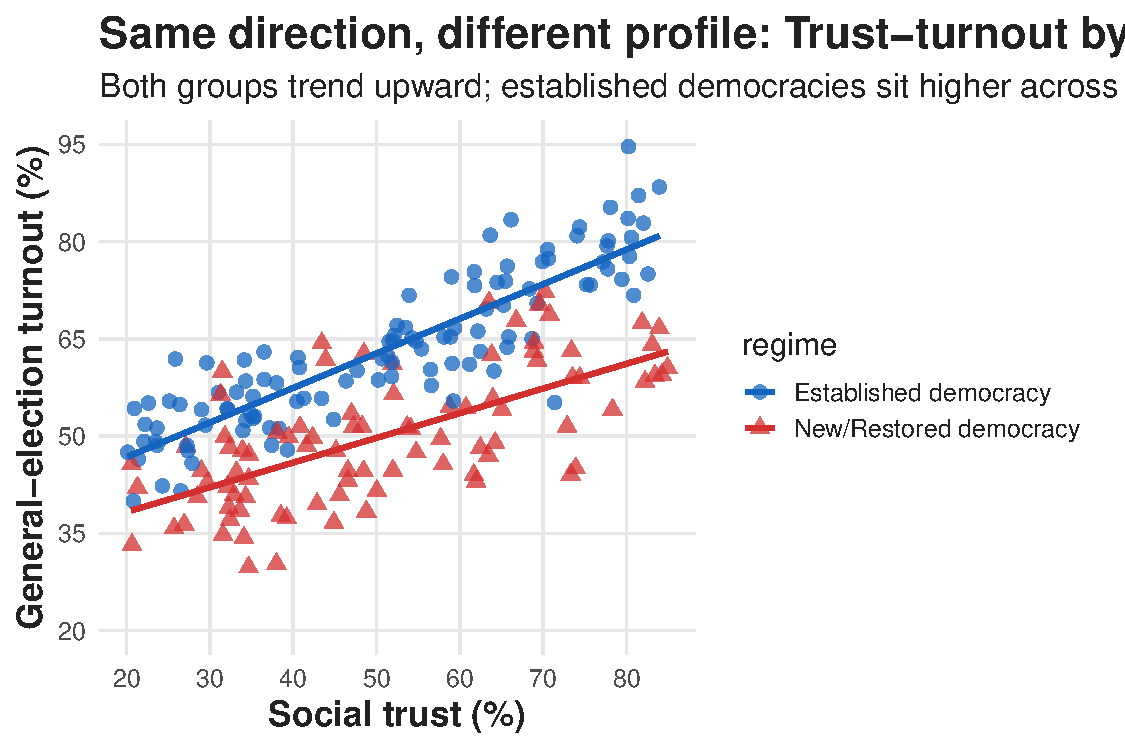
\includegraphics[keepaspectratio]{index_files/figure-pdf/fig-trust-turnout-grouped-1.pdf}}

}

\caption{\label{fig-trust-turnout-grouped}Social trust and
general-election turnout, grouped by regime type (synthetic). Each line
is an OLS fit within group.}

\end{figure}%

\subsection{Step-by-step computation of Pearson's r with a
table}\label{step-by-step-computation-of-pearsons-r-with-a-table}

\begin{Shaded}
\begin{Highlighting}[]
\CommentTok{\#| label: tbl{-}corr{-}handcalc}
\CommentTok{\#| tbl{-}cap: "Hand calculation of Pearson’s r: spending per voter (x) and turnout (y) across municipalities (synthetic)."}
\CommentTok{\#| message: false}
\CommentTok{\#| warning: false}

\FunctionTok{library}\NormalTok{(tibble)}
\FunctionTok{library}\NormalTok{(dplyr)}
\FunctionTok{library}\NormalTok{(knitr)}

\NormalTok{muni }\OtherTok{\textless{}{-}}\NormalTok{ tibble}\SpecialCharTok{::}\FunctionTok{tibble}\NormalTok{(}
  \AttributeTok{muni =} \FunctionTok{paste0}\NormalTok{(}\StringTok{"M"}\NormalTok{, }\DecValTok{1}\SpecialCharTok{:}\DecValTok{9}\NormalTok{),}
  \AttributeTok{spend\_per\_voter =} \FunctionTok{c}\NormalTok{(}\DecValTok{18}\NormalTok{, }\DecValTok{22}\NormalTok{, }\DecValTok{25}\NormalTok{, }\DecValTok{27}\NormalTok{, }\DecValTok{29}\NormalTok{, }\DecValTok{33}\NormalTok{, }\DecValTok{35}\NormalTok{, }\DecValTok{40}\NormalTok{, }\DecValTok{55}\NormalTok{),  }\CommentTok{\# USD}
  \AttributeTok{turnout\_pct      =} \FunctionTok{c}\NormalTok{(}\DecValTok{51}\NormalTok{, }\DecValTok{55}\NormalTok{, }\DecValTok{58}\NormalTok{, }\DecValTok{60}\NormalTok{, }\DecValTok{62}\NormalTok{, }\DecValTok{65}\NormalTok{, }\DecValTok{68}\NormalTok{, }\DecValTok{71}\NormalTok{, }\DecValTok{64}\NormalTok{)   }\CommentTok{\# \%}
\NormalTok{)}

\NormalTok{calc }\OtherTok{\textless{}{-}}\NormalTok{ muni }\SpecialCharTok{|\textgreater{}}
  \FunctionTok{mutate}\NormalTok{(}
    \AttributeTok{x   =}\NormalTok{ spend\_per\_voter,}
    \AttributeTok{y   =}\NormalTok{ turnout\_pct,}
    \AttributeTok{xbar =} \FunctionTok{mean}\NormalTok{(x), }\AttributeTok{ybar =} \FunctionTok{mean}\NormalTok{(y),}
    \AttributeTok{sx   =} \FunctionTok{sd}\NormalTok{(x),   }\AttributeTok{sy   =} \FunctionTok{sd}\NormalTok{(y),}
    \AttributeTok{x\_minus\_xbar =}\NormalTok{ x }\SpecialCharTok{{-}}\NormalTok{ xbar,}
    \AttributeTok{y\_minus\_ybar =}\NormalTok{ y }\SpecialCharTok{{-}}\NormalTok{ ybar,}
    \AttributeTok{zx =}\NormalTok{ (x }\SpecialCharTok{{-}}\NormalTok{ xbar)}\SpecialCharTok{/}\NormalTok{sx,}
    \AttributeTok{zy =}\NormalTok{ (y }\SpecialCharTok{{-}}\NormalTok{ ybar)}\SpecialCharTok{/}\NormalTok{sy,}
    \AttributeTok{zx\_zy =}\NormalTok{ zx }\SpecialCharTok{*}\NormalTok{ zy}
\NormalTok{  )}

\NormalTok{r\_hand }\OtherTok{\textless{}{-}} \FunctionTok{sum}\NormalTok{(calc}\SpecialCharTok{$}\NormalTok{zx\_zy) }\SpecialCharTok{/}\NormalTok{ (}\FunctionTok{nrow}\NormalTok{(calc) }\SpecialCharTok{{-}} \DecValTok{1}\NormalTok{)}

\NormalTok{calc }\SpecialCharTok{|\textgreater{}}
  \FunctionTok{transmute}\NormalTok{(}
    \AttributeTok{Municipality =}\NormalTok{ muni,}
    \StringTok{\textasciigrave{}}\AttributeTok{x (spend)}\StringTok{\textasciigrave{}} \OtherTok{=}\NormalTok{ x,}
    \StringTok{\textasciigrave{}}\AttributeTok{y (turnout)}\StringTok{\textasciigrave{}} \OtherTok{=}\NormalTok{ y,}
    \StringTok{\textasciigrave{}}\AttributeTok{x {-} x̄}\StringTok{\textasciigrave{}} \OtherTok{=} \FunctionTok{round}\NormalTok{(x\_minus\_xbar, }\DecValTok{2}\NormalTok{),}
    \StringTok{\textasciigrave{}}\AttributeTok{y {-} ȳ}\StringTok{\textasciigrave{}} \OtherTok{=} \FunctionTok{round}\NormalTok{(y\_minus\_ybar, }\DecValTok{2}\NormalTok{),}
    \StringTok{\textasciigrave{}}\AttributeTok{z\_x}\StringTok{\textasciigrave{}} \OtherTok{=} \FunctionTok{round}\NormalTok{(zx, }\DecValTok{3}\NormalTok{),}
    \StringTok{\textasciigrave{}}\AttributeTok{z\_y}\StringTok{\textasciigrave{}} \OtherTok{=} \FunctionTok{round}\NormalTok{(zy, }\DecValTok{3}\NormalTok{),}
    \StringTok{\textasciigrave{}}\AttributeTok{z\_x · z\_y}\StringTok{\textasciigrave{}} \OtherTok{=} \FunctionTok{round}\NormalTok{(zx\_zy, }\DecValTok{3}\NormalTok{)}
\NormalTok{  ) }\SpecialCharTok{|\textgreater{}}
  \FunctionTok{kable}\NormalTok{(}\AttributeTok{align =} \StringTok{"lrrrrrrr"}\NormalTok{, }\AttributeTok{caption =} \StringTok{"Components used to compute r"}\NormalTok{)}
\end{Highlighting}
\end{Shaded}

\begin{longtable}[]{@{}
  >{\raggedright\arraybackslash}p{(\linewidth - 14\tabcolsep) * \real{0.1781}}
  >{\raggedleft\arraybackslash}p{(\linewidth - 14\tabcolsep) * \real{0.1370}}
  >{\raggedleft\arraybackslash}p{(\linewidth - 14\tabcolsep) * \real{0.1644}}
  >{\raggedleft\arraybackslash}p{(\linewidth - 14\tabcolsep) * \real{0.0959}}
  >{\raggedleft\arraybackslash}p{(\linewidth - 14\tabcolsep) * \real{0.0959}}
  >{\raggedleft\arraybackslash}p{(\linewidth - 14\tabcolsep) * \real{0.0959}}
  >{\raggedleft\arraybackslash}p{(\linewidth - 14\tabcolsep) * \real{0.0959}}
  >{\raggedleft\arraybackslash}p{(\linewidth - 14\tabcolsep) * \real{0.1370}}@{}}
\caption{Components used to compute r}\tabularnewline
\toprule\noalign{}
\begin{minipage}[b]{\linewidth}\raggedright
Municipality
\end{minipage} & \begin{minipage}[b]{\linewidth}\raggedleft
x (spend)
\end{minipage} & \begin{minipage}[b]{\linewidth}\raggedleft
y (turnout)
\end{minipage} & \begin{minipage}[b]{\linewidth}\raggedleft
x - x̄
\end{minipage} & \begin{minipage}[b]{\linewidth}\raggedleft
y - ȳ
\end{minipage} & \begin{minipage}[b]{\linewidth}\raggedleft
z\_x
\end{minipage} & \begin{minipage}[b]{\linewidth}\raggedleft
z\_y
\end{minipage} & \begin{minipage}[b]{\linewidth}\raggedleft
z\_x · z\_y
\end{minipage} \\
\midrule\noalign{}
\endfirsthead
\toprule\noalign{}
\begin{minipage}[b]{\linewidth}\raggedright
Municipality
\end{minipage} & \begin{minipage}[b]{\linewidth}\raggedleft
x (spend)
\end{minipage} & \begin{minipage}[b]{\linewidth}\raggedleft
y (turnout)
\end{minipage} & \begin{minipage}[b]{\linewidth}\raggedleft
x - x̄
\end{minipage} & \begin{minipage}[b]{\linewidth}\raggedleft
y - ȳ
\end{minipage} & \begin{minipage}[b]{\linewidth}\raggedleft
z\_x
\end{minipage} & \begin{minipage}[b]{\linewidth}\raggedleft
z\_y
\end{minipage} & \begin{minipage}[b]{\linewidth}\raggedleft
z\_x · z\_y
\end{minipage} \\
\midrule\noalign{}
\endhead
\bottomrule\noalign{}
\endlastfoot
M1 & 18 & 51 & -13.56 & -10.56 & -1.225 & -1.674 & 2.050 \\
M2 & 22 & 55 & -9.56 & -6.56 & -0.863 & -1.039 & 0.897 \\
M3 & 25 & 58 & -6.56 & -3.56 & -0.592 & -0.564 & 0.334 \\
M4 & 27 & 60 & -4.56 & -1.56 & -0.412 & -0.247 & 0.102 \\
M5 & 29 & 62 & -2.56 & 0.44 & -0.231 & 0.070 & -0.016 \\
M6 & 33 & 65 & 1.44 & 3.44 & 0.130 & 0.546 & 0.071 \\
M7 & 35 & 68 & 3.44 & 6.44 & 0.311 & 1.022 & 0.318 \\
M8 & 40 & 71 & 8.44 & 9.44 & 0.763 & 1.497 & 1.142 \\
M9 & 55 & 64 & 23.44 & 2.44 & 2.118 & 0.388 & 0.821 \\
\end{longtable}

\begin{Shaded}
\begin{Highlighting}[]
\FunctionTok{c}\NormalTok{(}
  \AttributeTok{Pearson\_r\_by\_hand =} \FunctionTok{round}\NormalTok{(r\_hand, }\DecValTok{3}\NormalTok{),}
  \AttributeTok{Pearson\_r\_builtin =} \FunctionTok{round}\NormalTok{(}\FunctionTok{cor}\NormalTok{(muni}\SpecialCharTok{$}\NormalTok{spend\_per\_voter, muni}\SpecialCharTok{$}\NormalTok{turnout\_pct), }\DecValTok{3}\NormalTok{)}
\NormalTok{)}
\end{Highlighting}
\end{Shaded}

\begin{verbatim}
Pearson_r_by_hand Pearson_r_builtin 
            0.715             0.715 
\end{verbatim}

We simulate a moderate positive relationship between campaign spending
per voter and turnout, then add a single high-spending, low-turnout
outlier (e.g., a contest with unusual mobilization failure). The two
panels and the printed summary show how r shifts.

\begin{Shaded}
\begin{Highlighting}[]
\CommentTok{\#| label: fig{-}outlier{-}effect}
\CommentTok{\#| fig{-}cap: "A single unusual case can flatten the slope and drag Pearson’s r downward (synthetic)."}
\CommentTok{\#| fig{-}width: 8}
\CommentTok{\#| fig{-}height: 4.8}
\CommentTok{\#| dpi: 320}
\CommentTok{\#| message: false}
\CommentTok{\#| warning: false}

\FunctionTok{library}\NormalTok{(dplyr)}
\FunctionTok{library}\NormalTok{(ggplot2)}
\FunctionTok{library}\NormalTok{(scales)}

\NormalTok{theme\_textbook }\OtherTok{\textless{}{-}} \ControlFlowTok{function}\NormalTok{(}\AttributeTok{base\_size =} \DecValTok{15}\NormalTok{)\{}
  \FunctionTok{theme\_minimal}\NormalTok{(}\AttributeTok{base\_size =}\NormalTok{ base\_size) }\SpecialCharTok{+}
    \FunctionTok{theme}\NormalTok{(}
      \AttributeTok{text =} \FunctionTok{element\_text}\NormalTok{(}\AttributeTok{color =} \StringTok{"\#222"}\NormalTok{),}
      \AttributeTok{axis.title =} \FunctionTok{element\_text}\NormalTok{(}\AttributeTok{face =} \StringTok{"bold"}\NormalTok{, }\AttributeTok{size =}\NormalTok{ base\_size }\SpecialCharTok{+} \DecValTok{2}\NormalTok{),}
      \AttributeTok{plot.title =} \FunctionTok{element\_text}\NormalTok{(}\AttributeTok{face =} \StringTok{"bold"}\NormalTok{, }\AttributeTok{size =}\NormalTok{ base\_size }\SpecialCharTok{+} \DecValTok{6}\NormalTok{),}
      \AttributeTok{plot.subtitle =} \FunctionTok{element\_text}\NormalTok{(}\AttributeTok{size =}\NormalTok{ base\_size }\SpecialCharTok{+} \DecValTok{1}\NormalTok{),}
      \AttributeTok{panel.grid.major =} \FunctionTok{element\_line}\NormalTok{(}\AttributeTok{color =} \StringTok{"\#e6e6e6"}\NormalTok{, }\AttributeTok{linewidth =} \FloatTok{0.6}\NormalTok{),}
      \AttributeTok{panel.grid.minor =} \FunctionTok{element\_blank}\NormalTok{(),}
      \AttributeTok{plot.margin =} \FunctionTok{margin}\NormalTok{(}\DecValTok{8}\NormalTok{, }\DecValTok{14}\NormalTok{, }\DecValTok{8}\NormalTok{, }\DecValTok{8}\NormalTok{)}
\NormalTok{    )}
\NormalTok{\}}

\FunctionTok{set.seed}\NormalTok{(}\DecValTok{202}\NormalTok{)}
\NormalTok{n }\OtherTok{\textless{}{-}} \DecValTok{120}
\NormalTok{base }\OtherTok{\textless{}{-}}\NormalTok{ tibble}\SpecialCharTok{::}\FunctionTok{tibble}\NormalTok{(}
  \AttributeTok{spend   =} \FunctionTok{runif}\NormalTok{(n, }\DecValTok{5}\NormalTok{, }\DecValTok{55}\NormalTok{),}
  \AttributeTok{turnout =} \DecValTok{40} \SpecialCharTok{+} \FloatTok{0.45}\SpecialCharTok{*}\NormalTok{spend }\SpecialCharTok{+} \FunctionTok{rnorm}\NormalTok{(n, }\DecValTok{0}\NormalTok{, }\DecValTok{6}\NormalTok{)}
\NormalTok{) }\SpecialCharTok{|\textgreater{}}
  \FunctionTok{mutate}\NormalTok{(}\AttributeTok{turnout =} \FunctionTok{pmin}\NormalTok{(}\FunctionTok{pmax}\NormalTok{(turnout, }\DecValTok{25}\NormalTok{), }\DecValTok{90}\NormalTok{))}

\NormalTok{df0 }\OtherTok{\textless{}{-}}\NormalTok{ base }\SpecialCharTok{|\textgreater{}}
  \FunctionTok{mutate}\NormalTok{(}\AttributeTok{spec =} \StringTok{"Without outlier"}\NormalTok{, }\AttributeTok{is\_outlier =} \ConstantTok{FALSE}\NormalTok{)}

\NormalTok{df1\_base }\OtherTok{\textless{}{-}}\NormalTok{ base }\SpecialCharTok{|\textgreater{}}
  \FunctionTok{mutate}\NormalTok{(}\AttributeTok{spec =} \StringTok{"With outlier"}\NormalTok{, }\AttributeTok{is\_outlier =} \ConstantTok{FALSE}\NormalTok{)}

\NormalTok{outlier }\OtherTok{\textless{}{-}}\NormalTok{ tibble}\SpecialCharTok{::}\FunctionTok{tibble}\NormalTok{(}
  \AttributeTok{spend =} \DecValTok{60}\NormalTok{, }\AttributeTok{turnout =} \DecValTok{45}\NormalTok{, }\AttributeTok{spec =} \StringTok{"With outlier"}\NormalTok{, }\AttributeTok{is\_outlier =} \ConstantTok{TRUE}
\NormalTok{)}

\NormalTok{combined }\OtherTok{\textless{}{-}} \FunctionTok{bind\_rows}\NormalTok{(df0, df1\_base, outlier)}

\NormalTok{r\_stats }\OtherTok{\textless{}{-}}\NormalTok{ combined }\SpecialCharTok{|\textgreater{}}
  \FunctionTok{group\_by}\NormalTok{(spec) }\SpecialCharTok{|\textgreater{}}
  \FunctionTok{summarise}\NormalTok{(}\AttributeTok{r =} \FunctionTok{cor}\NormalTok{(spend, turnout), }\AttributeTok{.groups =} \StringTok{"drop"}\NormalTok{)}

\NormalTok{ann }\OtherTok{\textless{}{-}}\NormalTok{ combined }\SpecialCharTok{|\textgreater{}}
  \FunctionTok{group\_by}\NormalTok{(spec) }\SpecialCharTok{|\textgreater{}}
  \FunctionTok{summarise}\NormalTok{(}\AttributeTok{x =} \FunctionTok{min}\NormalTok{(spend) }\SpecialCharTok{+} \FloatTok{1.5}\NormalTok{, }\AttributeTok{y =} \FunctionTok{max}\NormalTok{(turnout) }\SpecialCharTok{{-}} \DecValTok{2}\NormalTok{, }\AttributeTok{.groups =} \StringTok{"drop"}\NormalTok{) }\SpecialCharTok{|\textgreater{}}
  \FunctionTok{left\_join}\NormalTok{(r\_stats, }\AttributeTok{by =} \StringTok{"spec"}\NormalTok{) }\SpecialCharTok{|\textgreater{}}
  \FunctionTok{mutate}\NormalTok{(}\AttributeTok{label =} \FunctionTok{sprintf}\NormalTok{(}\StringTok{"r = \%.2f"}\NormalTok{, r))}

\FunctionTok{ggplot}\NormalTok{(combined, }\FunctionTok{aes}\NormalTok{(spend, turnout)) }\SpecialCharTok{+}
  \FunctionTok{geom\_point}\NormalTok{(}\FunctionTok{aes}\NormalTok{(}\AttributeTok{color =}\NormalTok{ is\_outlier), }\AttributeTok{alpha =}\NormalTok{ .}\DecValTok{85}\NormalTok{, }\AttributeTok{size =} \FloatTok{2.6}\NormalTok{) }\SpecialCharTok{+}
  \FunctionTok{scale\_color\_manual}\NormalTok{(}\AttributeTok{values =} \FunctionTok{c}\NormalTok{(}\StringTok{\textasciigrave{}}\AttributeTok{FALSE}\StringTok{\textasciigrave{}} \OtherTok{=} \StringTok{"\#2b2b2b"}\NormalTok{, }\StringTok{\textasciigrave{}}\AttributeTok{TRUE}\StringTok{\textasciigrave{}} \OtherTok{=} \StringTok{"\#D32F2F"}\NormalTok{), }\AttributeTok{guide =} \StringTok{"none"}\NormalTok{) }\SpecialCharTok{+}
  \FunctionTok{geom\_smooth}\NormalTok{(}\AttributeTok{method =} \StringTok{"lm"}\NormalTok{, }\AttributeTok{se =} \ConstantTok{TRUE}\NormalTok{, }\AttributeTok{color =} \StringTok{"\#1565C0"}\NormalTok{,}
              \AttributeTok{fill =} \FunctionTok{alpha}\NormalTok{(}\StringTok{"\#1565C0"}\NormalTok{, }\FloatTok{0.12}\NormalTok{), }\AttributeTok{linewidth =} \FloatTok{1.1}\NormalTok{) }\SpecialCharTok{+}
  \FunctionTok{geom\_label}\NormalTok{(}\AttributeTok{data =}\NormalTok{ ann, }\FunctionTok{aes}\NormalTok{(}\AttributeTok{x =}\NormalTok{ x, }\AttributeTok{y =}\NormalTok{ y, }\AttributeTok{label =}\NormalTok{ label),}
             \AttributeTok{size =} \FloatTok{3.6}\NormalTok{, }\AttributeTok{hjust =} \DecValTok{0}\NormalTok{, }\AttributeTok{vjust =} \DecValTok{1}\NormalTok{,}
             \AttributeTok{label.size =} \DecValTok{0}\NormalTok{, }\AttributeTok{color =} \StringTok{"\#333333"}\NormalTok{, }\AttributeTok{fill =} \FunctionTok{alpha}\NormalTok{(}\StringTok{"\#f5f5f5"}\NormalTok{, }\FloatTok{0.9}\NormalTok{)) }\SpecialCharTok{+}
  \FunctionTok{labs}\NormalTok{(}
    \AttributeTok{x =} \StringTok{"Campaign spending per voter (USD)"}\NormalTok{,}
    \AttributeTok{y =} \StringTok{"Turnout (\%)"}\NormalTok{,}
    \AttributeTok{title =} \StringTok{"Outliers can materially shrink linear association"}
\NormalTok{  ) }\SpecialCharTok{+}
  \FunctionTok{scale\_x\_continuous}\NormalTok{(}\AttributeTok{limits =} \FunctionTok{c}\NormalTok{(}\DecValTok{5}\NormalTok{, }\DecValTok{60}\NormalTok{), }\AttributeTok{breaks =} \FunctionTok{seq}\NormalTok{(}\DecValTok{5}\NormalTok{, }\DecValTok{60}\NormalTok{, }\DecValTok{10}\NormalTok{)) }\SpecialCharTok{+}
  \FunctionTok{scale\_y\_continuous}\NormalTok{(}\AttributeTok{limits =} \FunctionTok{c}\NormalTok{(}\DecValTok{25}\NormalTok{, }\DecValTok{90}\NormalTok{), }\AttributeTok{breaks =} \FunctionTok{seq}\NormalTok{(}\DecValTok{30}\NormalTok{, }\DecValTok{90}\NormalTok{, }\DecValTok{10}\NormalTok{)) }\SpecialCharTok{+}
  \FunctionTok{facet\_wrap}\NormalTok{(}\SpecialCharTok{\textasciitilde{}}\NormalTok{ spec, }\AttributeTok{ncol =} \DecValTok{2}\NormalTok{) }\SpecialCharTok{+}
  \FunctionTok{theme\_textbook}\NormalTok{()}
\end{Highlighting}
\end{Shaded}

\pandocbounded{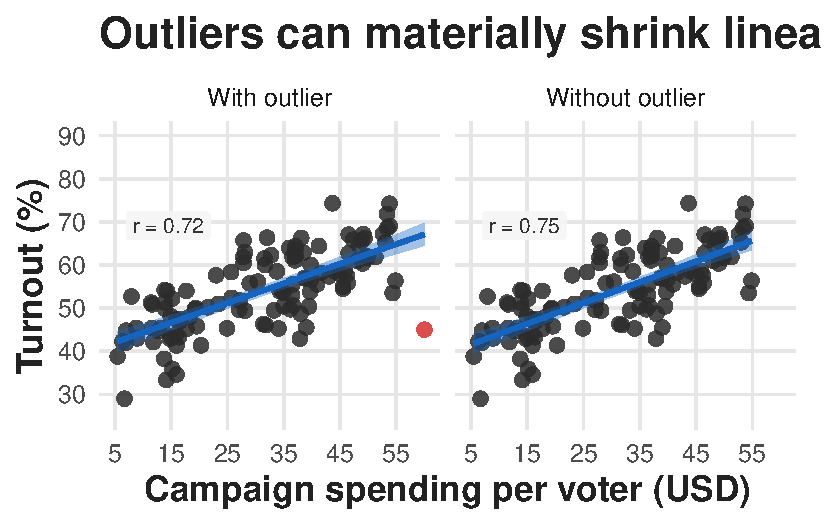
\includegraphics[keepaspectratio]{index_files/figure-pdf/unnamed-chunk-32-1.pdf}}

\begin{Shaded}
\begin{Highlighting}[]
\CommentTok{\#| label: tbl{-}outlier{-}summary}
\NormalTok{combined }\SpecialCharTok{|\textgreater{}}
  \FunctionTok{group\_by}\NormalTok{(spec) }\SpecialCharTok{|\textgreater{}}
  \FunctionTok{summarise}\NormalTok{(}\AttributeTok{Pearson\_r =} \FunctionTok{round}\NormalTok{(}\FunctionTok{cor}\NormalTok{(spend, turnout), }\DecValTok{3}\NormalTok{), }\AttributeTok{.groups =} \StringTok{"drop"}\NormalTok{) }\SpecialCharTok{|\textgreater{}}
  \FunctionTok{rename}\NormalTok{(}\AttributeTok{Specification =}\NormalTok{ spec)}
\end{Highlighting}
\end{Shaded}

\begin{verbatim}
# A tibble: 2 x 2
  Specification   Pearson_r
  <chr>               <dbl>
1 With outlier        0.717
2 Without outlier     0.749
\end{verbatim}

\section{Correlation via
Standardization}\label{correlation-via-standardization}

As noted, the first to compute correlation between two variables is to
compute theri meens. \[
z_{x,i} = \frac{x_i - \bar{x}}{s_x}, \qquad
z_{y,i} = \frac{y_i - \bar{y}}{s_y}
\] Once we compute the means, we then need to calcultate standard
deviation for each variable. \[
s_x = \sqrt{\frac{1}{n-1}\sum_{i=1}^{n} (x_i - \bar{x})^2}, \qquad
s_y = \sqrt{\frac{1}{n-1}\sum_{i=1}^{n} (y_i - \bar{y})^2}
\] Then, by plugging in the formula below, we then can compute the
r-correlation coefficient.

\[
r = \frac{1}{n-1}\sum_{i=1}^{n}
\left(\frac{x_i-\bar{x}}{s_x}\right)
\left(\frac{y_i-\bar{y}}{s_y}\right)
= \frac{1}{(n-1)s_x s_y}\sum_{i=1}^{n}(x_i-\bar{x})(y_i-\bar{y})
\]

\section{Correlation via Standardization: Definitions, Steps, and
Interpretation}\label{correlation-via-standardization-definitions-steps-and-interpretation}

\subsection{Notation and sample
summaries}\label{notation-and-sample-summaries}

We observe two quantitative variables for cases (i=1,\ldots,n): (x\_i)
and (y\_i). The sample means and (unbiased) sample standard deviations
are

\[
\bar{x}=\frac{1}{n}\sum_{i=1}^n x_i,
\qquad
\bar{y}=\frac{1}{n}\sum_{i=1}^n y_i,
\]

\[
s_x=\sqrt{\frac{1}{n-1}\sum_{i=1}^n (x_i-\bar{x})^2},
\qquad
s_y=\sqrt{\frac{1}{n-1}\sum_{i=1}^n (y_i-\bar{y})^2}.
\]

\textbf{What these do.} (\bar\{x\}) (resp. (\bar\{y\})) centers the
data; (s\_x) (resp. (s\_y)) measures average spread about the mean using
the (n-1) denominator so that sample variance is unbiased under IID
sampling.

\subsection{Standardization
(z-scores)}\label{standardization-z-scores-1}

To place (x) and (y) on common, unit-free scales, define the
standardized scores

\[
z_{x,i}=\frac{x_i-\bar{x}}{s_x},
\qquad
z_{y,i}=\frac{y_i-\bar{y}}{s_y}.
\]

\textbf{What this does.} Each (z) says ``how many (s)'s from the mean''
a case lies. Standardization ensures (\sum\emph{i z}\{x,i\}=0),
(\sum\emph{i z}\{x,i\}\^{}2=n-1) (and likewise for (y)), which makes the
correlation unit-free.

\begin{center}\rule{0.5\linewidth}{0.5pt}\end{center}

\subsection{Covariance (cross-deviation
average)}\label{covariance-cross-deviation-average}

The sample covariance aggregates the co-movement of centered variables:

\[
\operatorname{cov}(x,y)
=\frac{1}{n-1}\sum_{i=1}^n (x_i-\bar{x})(y_i-\bar{y}).
\]

\textbf{What this does.} Positive terms arise when (x\_i) and (y\_i) are
both above/below their means; negative terms arise when one is above and
the other below. Magnitude depends on the original units.

\begin{center}\rule{0.5\linewidth}{0.5pt}\end{center}

\subsection{Pearson correlation (three equivalent
forms)}\label{pearson-correlation-three-equivalent-forms}

\begin{enumerate}
\def\labelenumi{\arabic{enumi})}
\item
  \textbf{Mean product of standardized scores} \[
  r=\frac{1}{n-1}\sum_{i=1}^n z_{x,i}\,z_{y,i}.
  \]
\item
  \textbf{Scaled covariance} \[
  r=\frac{\operatorname{cov}(x,y)}{s_x\,s_y}.
  \]
\item
  \textbf{Shortcut using sums} \[
  r=\frac{\sum_{i=1}^n x_i y_i - n\,\bar{x}\,\bar{y}}
  {(n-1)\,s_x\,s_y}.
  \]
\end{enumerate}

\textbf{What these do.} (1) is most interpretable: average comovement
\emph{in SD units}. (2) rescales covariance to remove units. (3) is
algebraically identical and useful for checking work or computing by
hand.

\begin{center}\rule{0.5\linewidth}{0.5pt}\end{center}

\subsection{How to compute (r) step-by-step (exactly what your table
shows)}\label{how-to-compute-r-step-by-step-exactly-what-your-table-shows}

\begin{enumerate}
\def\labelenumi{\arabic{enumi}.}
\tightlist
\item
  \textbf{Center each variable}: compute deviations (x\_i-\bar\{x\}) and
  (y\_i-\bar\{y\}).
\item
  \textbf{Standardize}: compute (A\_i=z\_\{x,i\}=(x\_i-\bar\{x\})/s\_x)
  and (B\_i=z\_\{y,i\}=(y\_i-\bar\{y\})/s\_y).
\item
  \textbf{Multiply standardized pairs}: compute (A\_i B\_i).
\item
  \textbf{Average the products} with the (n-1) denominator: \[
  r=\frac{1}{n-1}\sum_{i=1}^n A_i B_i.
  \]
\end{enumerate}

\textbf{How to read the last column.} If many (A\_i B\_i) are negative,
large positive (x) tends to pair with low (y) (and vice versa), giving a
negative (r). If they are mostly positive, the association is positive.

\begin{center}\rule{0.5\linewidth}{0.5pt}\end{center}

\subsection{Properties and
interpretation}\label{properties-and-interpretation}

\begin{itemize}
\tightlist
\item
  \textbf{Range:} (r\in[-1,1]). (\textbar r\textbar=1) only for perfect
  straight-line patterns; (r=0) means \emph{no linear} association.
\item
  \textbf{Direction \& strength:} the \textbf{sign} gives direction;
  (\textbar r\textbar) gauges linear tightness (larger
  (\textbar r\textbar) → tighter cloud).
\item
  \textbf{Unit-free \& symmetric:} (r) is unchanged by linear rescaling
  of either variable and by swapping (x) and (y).
\item
  \textbf{Use with care:} (r) summarizes \textbf{linear} association; it
  can be distorted by outliers and is inappropriate for clearly
  non-linear patterns (consider rank-based (\rho) or (\tau) then).
\end{itemize}

\bookmarksetup{startatroot}

\chapter{Chapter 5:Two-Way Tables}\label{chapter-5two-way-tables}

A two-way table, also called a contingency table, is a statistical tool
used to organize and display data involving two categorical variables
simultaneously. The table arranges data in a grid format where one
variable's categories form the rows and the other variable's categories
form the columns, with each cell showing the frequency or count of
observations that fall into both categories. For example, a two-way
table might show the relationship between gender (male/female) and
preference for a product (like/dislike), with counts in each cell
representing how many people of each gender expressed each preference.
These tables are particularly valuable because they allow researchers to
examine patterns, relationships, and potential associations between the
two variables at a glance. The margins of the table typically include
row totals and column totals, which summarize the data for each
individual category, while the overall total appears in the corner.
Two-way tables serve as the foundation for various statistical analyses,
including chi-square tests for independence, and they make it easier to
calculate conditional probabilities and identify trends within
categorical data sets.

\begin{longtable}[]{@{}lrrr@{}}
\caption{Two-way table of marital status and football
preferences}\label{tbl-football}\tabularnewline
\toprule\noalign{}
Marital Status & Like Football & Don't Like Football & Total \\
\midrule\noalign{}
\endfirsthead
\toprule\noalign{}
Marital Status & Like Football & Don't Like Football & Total \\
\midrule\noalign{}
\endhead
\bottomrule\noalign{}
\endlastfoot
Single & 178 & 133 & 311 \\
Married & 60 & 29 & 89 \\
\textbf{Total} & \textbf{238} & \textbf{162} & \textbf{400} \\
\end{longtable}

These percentages reveal that married students (67.4\%) are more likely
than single students (57.2\%) to enjoy watching professional
football---a difference of about 10 percentage points.

Among single students, that would be:

\[
\frac{178}{311} \times 100
\]

Among married students, the calculation would be:

\[
\frac{39}{67} \times 100
\]

Percentaging within rows in this way ensures that we are comparing like
with like---that is, comparing preferences across marital
categories.What are the categoies that matter

It is also useful to distinguish between \textbf{marginal},
\textbf{conditional}, and \textbf{cell} percentages.\\
A \emph{marginal percentage} uses totals along the margins of a
table---for instance, the proportion of students who are married:

\[
\frac{67}{378} \times 100
\]

A \emph{conditional percentage} is calculated within a specific
category, such as the percentage of married students who like football:

\[
\frac{39}{67} \times 100
\]

Finally, a \emph{cell percentage} divides the frequency in a single cell
by the grand total:

\[
\frac{28}{378} \times 100
\]

We could visualize a contingency table using a `mosaic plot' in
R-Studio. A mosaic plot displays the joint distribution of marital
status and football preference. The total width of each column is
proportional to the number of respondents who either like or do not like
football, while the height of each colored segment within a column
reflects the share of singles versus married individuals among that
preference group. Within the ``Like Football'\,' column, 178 of 238
respondents (74.8\%) are single and 60 (25.2\%) are married; within the
``Don't Like Football'\,' column, 133 of 162 respondents (82.1\%) are
single and 29 (17.9\%) are married. Thus, although singles dominate both
preference groups numerically, the relative composition differs slightly
across them, and the mosaic layout allows this departure from
independence to be seen directly in area rather than inferred from raw
counts alone.

\begin{Shaded}
\begin{Highlighting}[]
\CommentTok{\#| label: fig{-}football{-}mosaic{-}labeled}
\CommentTok{\#| fig{-}cap: "Mosaic plot of Marital Status × Football Preference with counts and within{-}column percentages."}
\CommentTok{\#| fig{-}width: 8}
\CommentTok{\#| fig{-}height: 5}
\CommentTok{\#| warning: false}
\CommentTok{\#| message: false}

\FunctionTok{suppressPackageStartupMessages}\NormalTok{(\{}
  \FunctionTok{library}\NormalTok{(dplyr); }\FunctionTok{library}\NormalTok{(ggplot2); }\FunctionTok{library}\NormalTok{(scales); }\FunctionTok{library}\NormalTok{(tidyr)}
\NormalTok{\})}

\CommentTok{\# {-}{-}{-}{-}{-}{-}{-}{-}{-}{-}{-}{-}{-} data {-}{-}{-}{-}{-}{-}{-}{-}{-}{-}{-}{-}{-}}
\NormalTok{df }\OtherTok{\textless{}{-}}\NormalTok{ tibble}\SpecialCharTok{::}\FunctionTok{tribble}\NormalTok{(}
  \SpecialCharTok{\textasciitilde{}}\NormalTok{MaritalStatus, }\SpecialCharTok{\textasciitilde{}}\NormalTok{Preference,            }\SpecialCharTok{\textasciitilde{}}\NormalTok{n,}
  \StringTok{"Single"}\NormalTok{,       }\StringTok{"Like Football"}\NormalTok{,        }\DecValTok{178}\NormalTok{,}
  \StringTok{"Single"}\NormalTok{,       }\StringTok{"Don\textquotesingle{}t Like Football"}\NormalTok{,  }\DecValTok{133}\NormalTok{,}
  \StringTok{"Married"}\NormalTok{,      }\StringTok{"Like Football"}\NormalTok{,         }\DecValTok{60}\NormalTok{,}
  \StringTok{"Married"}\NormalTok{,      }\StringTok{"Don\textquotesingle{}t Like Football"}\NormalTok{,   }\DecValTok{29}
\NormalTok{) }\SpecialCharTok{|\textgreater{}}
  \FunctionTok{mutate}\NormalTok{(}
    \AttributeTok{MaritalStatus =} \FunctionTok{factor}\NormalTok{(MaritalStatus, }\AttributeTok{levels =} \FunctionTok{c}\NormalTok{(}\StringTok{"Single"}\NormalTok{,}\StringTok{"Married"}\NormalTok{)),}
    \AttributeTok{Preference    =} \FunctionTok{factor}\NormalTok{(Preference,    }\AttributeTok{levels =} \FunctionTok{c}\NormalTok{(}\StringTok{"Like Football"}\NormalTok{,}\StringTok{"Don\textquotesingle{}t Like Football"}\NormalTok{))}
\NormalTok{  )}

\CommentTok{\# {-}{-}{-}{-}{-}{-}{-}{-}{-}{-}{-}{-}{-} parameters you can tweak {-}{-}{-}{-}{-}{-}{-}{-}{-}{-}{-}{-}{-}}
\NormalTok{label\_count\_size }\OtherTok{\textless{}{-}} \FloatTok{4.6}
\NormalTok{label\_pct\_size   }\OtherTok{\textless{}{-}} \FloatTok{3.8}
\NormalTok{axis\_title\_size  }\OtherTok{\textless{}{-}} \DecValTok{16}
\NormalTok{axis\_text\_size   }\OtherTok{\textless{}{-}} \DecValTok{13}
\NormalTok{title\_size       }\OtherTok{\textless{}{-}} \DecValTok{18}

 
\NormalTok{grand\_total }\OtherTok{\textless{}{-}} \FunctionTok{sum}\NormalTok{(df}\SpecialCharTok{$}\NormalTok{n)}

\NormalTok{col\_info }\OtherTok{\textless{}{-}}\NormalTok{ df }\SpecialCharTok{|\textgreater{}}
  \FunctionTok{group\_by}\NormalTok{(Preference) }\SpecialCharTok{|\textgreater{}}
  \FunctionTok{summarise}\NormalTok{(}\AttributeTok{col\_n =} \FunctionTok{sum}\NormalTok{(n), }\AttributeTok{.groups =} \StringTok{"drop"}\NormalTok{) }\SpecialCharTok{|\textgreater{}}
  \FunctionTok{mutate}\NormalTok{(}
    \AttributeTok{width =}\NormalTok{ col\_n }\SpecialCharTok{/}\NormalTok{ grand\_total,}
    \AttributeTok{xmin  =} \FunctionTok{lag}\NormalTok{(}\FunctionTok{cumsum}\NormalTok{(width), }\AttributeTok{default =} \DecValTok{0}\NormalTok{),}
    \AttributeTok{xmax  =} \FunctionTok{cumsum}\NormalTok{(width),}
    \AttributeTok{xmid  =}\NormalTok{ (xmin }\SpecialCharTok{+}\NormalTok{ xmax) }\SpecialCharTok{/} \DecValTok{2}
\NormalTok{  )}

\NormalTok{rects }\OtherTok{\textless{}{-}}\NormalTok{ df }\SpecialCharTok{|\textgreater{}}
  \FunctionTok{left\_join}\NormalTok{(col\_info, }\AttributeTok{by =} \StringTok{"Preference"}\NormalTok{) }\SpecialCharTok{|\textgreater{}}
  \FunctionTok{group\_by}\NormalTok{(Preference) }\SpecialCharTok{|\textgreater{}}
  \FunctionTok{mutate}\NormalTok{(}
    \AttributeTok{col\_prop  =}\NormalTok{ n }\SpecialCharTok{/} \FunctionTok{sum}\NormalTok{(n),}
    \AttributeTok{ymin      =} \FunctionTok{lag}\NormalTok{(}\FunctionTok{cumsum}\NormalTok{(col\_prop), }\AttributeTok{default =} \DecValTok{0}\NormalTok{),}
    \AttributeTok{ymax      =} \FunctionTok{cumsum}\NormalTok{(col\_prop),}
    \AttributeTok{ymid      =}\NormalTok{ (ymin }\SpecialCharTok{+}\NormalTok{ ymax) }\SpecialCharTok{/} \DecValTok{2}\NormalTok{,}
    \AttributeTok{pct\_lab   =} \FunctionTok{percent}\NormalTok{(col\_prop, }\AttributeTok{accuracy =} \FloatTok{0.1}\NormalTok{),}
    \AttributeTok{count\_lab =} \FunctionTok{sprintf}\NormalTok{(}\StringTok{"\%d"}\NormalTok{, n)}
\NormalTok{  ) }\SpecialCharTok{|\textgreater{}}
  \FunctionTok{ungroup}\NormalTok{()}

\NormalTok{fills }\OtherTok{\textless{}{-}} \FunctionTok{c}\NormalTok{(}\StringTok{"Single"} \OtherTok{=} \StringTok{"\#4C78A8"}\NormalTok{, }\StringTok{"Married"} \OtherTok{=} \StringTok{"\#F58518"}\NormalTok{)}

\NormalTok{p }\OtherTok{\textless{}{-}} \FunctionTok{ggplot}\NormalTok{(rects) }\SpecialCharTok{+}
  \CommentTok{\# tiles}
  \FunctionTok{geom\_rect}\NormalTok{(}\FunctionTok{aes}\NormalTok{(}\AttributeTok{xmin =}\NormalTok{ xmin, }\AttributeTok{xmax =}\NormalTok{ xmax, }\AttributeTok{ymin =}\NormalTok{ ymin, }\AttributeTok{ymax =}\NormalTok{ ymax,}
                \AttributeTok{fill =}\NormalTok{ MaritalStatus),}
            \AttributeTok{color =} \StringTok{"white"}\NormalTok{, }\AttributeTok{linewidth =} \FloatTok{0.9}\NormalTok{) }\SpecialCharTok{+}
  \CommentTok{\# counts (bigger)}
  \FunctionTok{geom\_text}\NormalTok{(}\FunctionTok{aes}\NormalTok{(}\AttributeTok{x =}\NormalTok{ (xmin}\SpecialCharTok{+}\NormalTok{xmax)}\SpecialCharTok{/}\DecValTok{2}\NormalTok{, }\AttributeTok{y =}\NormalTok{ ymid, }\AttributeTok{label =}\NormalTok{ count\_lab),}
            \AttributeTok{fontface =} \StringTok{"bold"}\NormalTok{, }\AttributeTok{size =}\NormalTok{ label\_count\_size, }\AttributeTok{vjust =} \FloatTok{0.1}\NormalTok{) }\SpecialCharTok{+}
  \CommentTok{\# percentages (smaller, just below)}
  \FunctionTok{geom\_text}\NormalTok{(}\FunctionTok{aes}\NormalTok{(}\AttributeTok{x =}\NormalTok{ (xmin}\SpecialCharTok{+}\NormalTok{xmax)}\SpecialCharTok{/}\DecValTok{2}\NormalTok{, }\AttributeTok{y =}\NormalTok{ ymid, }\AttributeTok{label =}\NormalTok{ pct\_lab),}
            \AttributeTok{size =}\NormalTok{ label\_pct\_size, }\AttributeTok{vjust =} \FloatTok{1.6}\NormalTok{) }\SpecialCharTok{+}
  \CommentTok{\# x labels at column centers}
  \FunctionTok{geom\_text}\NormalTok{(}\AttributeTok{data =} \FunctionTok{distinct}\NormalTok{(col\_info, Preference, xmid),}
            \FunctionTok{aes}\NormalTok{(}\AttributeTok{x =}\NormalTok{ xmid, }\AttributeTok{y =} \SpecialCharTok{{-}}\FloatTok{0.045}\NormalTok{, }\AttributeTok{label =}\NormalTok{ Preference),}
            \AttributeTok{fontface =} \StringTok{"bold"}\NormalTok{, }\AttributeTok{size =}\NormalTok{ axis\_text\_size}\SpecialCharTok{/}\DecValTok{3}\NormalTok{, }\AttributeTok{vjust =} \DecValTok{1}\NormalTok{) }\SpecialCharTok{+}
  \FunctionTok{scale\_x\_continuous}\NormalTok{(}\AttributeTok{limits =} \FunctionTok{c}\NormalTok{(}\DecValTok{0}\NormalTok{,}\DecValTok{1}\NormalTok{), }\AttributeTok{expand =} \FunctionTok{c}\NormalTok{(}\DecValTok{0}\NormalTok{,}\DecValTok{0}\NormalTok{), }\AttributeTok{breaks =} \ConstantTok{NULL}\NormalTok{) }\SpecialCharTok{+}
  \FunctionTok{scale\_y\_continuous}\NormalTok{(}\AttributeTok{limits =} \FunctionTok{c}\NormalTok{(}\SpecialCharTok{{-}}\FloatTok{0.06}\NormalTok{,}\DecValTok{1}\NormalTok{), }\AttributeTok{expand =} \FunctionTok{c}\NormalTok{(}\DecValTok{0}\NormalTok{,}\DecValTok{0}\NormalTok{),}
                     \AttributeTok{labels =} \FunctionTok{percent\_format}\NormalTok{(}\AttributeTok{accuracy =} \DecValTok{1}\NormalTok{)) }\SpecialCharTok{+}
  \FunctionTok{scale\_fill\_manual}\NormalTok{(}\AttributeTok{values =}\NormalTok{ fills) }\SpecialCharTok{+}
  \FunctionTok{labs}\NormalTok{(}
    \AttributeTok{x =} \StringTok{"Football Preference"}\NormalTok{,}
    \AttributeTok{y =} \StringTok{"Marital{-}Status Share d d"}\NormalTok{,}
    \AttributeTok{title =} \StringTok{"Marital Status × Football Preference — Mosaic"}
\NormalTok{  ) }\SpecialCharTok{+}
  \FunctionTok{theme\_minimal}\NormalTok{(}\AttributeTok{base\_size =}\NormalTok{ axis\_text\_size) }\SpecialCharTok{+}
  \FunctionTok{theme}\NormalTok{(}
    \AttributeTok{plot.title   =} \FunctionTok{element\_text}\NormalTok{(}\AttributeTok{face =} \StringTok{"bold"}\NormalTok{, }\AttributeTok{size =}\NormalTok{ title\_size, }\AttributeTok{hjust =} \FloatTok{0.5}\NormalTok{),}
    \AttributeTok{axis.title.x =} \FunctionTok{element\_text}\NormalTok{(}\AttributeTok{size =}\NormalTok{ axis\_title\_size, }\AttributeTok{margin =} \FunctionTok{margin}\NormalTok{(}\AttributeTok{t =} \DecValTok{10}\NormalTok{)),}
    \AttributeTok{axis.title.y =} \FunctionTok{element\_text}\NormalTok{(}\AttributeTok{size =}\NormalTok{ axis\_title\_size, }\AttributeTok{margin =} \FunctionTok{margin}\NormalTok{(}\AttributeTok{r =} \DecValTok{10}\NormalTok{)),}
    \AttributeTok{axis.text    =} \FunctionTok{element\_text}\NormalTok{(}\AttributeTok{size =}\NormalTok{ axis\_text\_size),}
    \AttributeTok{panel.grid   =} \FunctionTok{element\_blank}\NormalTok{(),}
    \AttributeTok{legend.title =} \FunctionTok{element\_text}\NormalTok{(}\AttributeTok{face =} \StringTok{"bold"}\NormalTok{),}
    \AttributeTok{legend.position =} \StringTok{"right"}
\NormalTok{  )}

\NormalTok{p}
\end{Highlighting}
\end{Shaded}

\pandocbounded{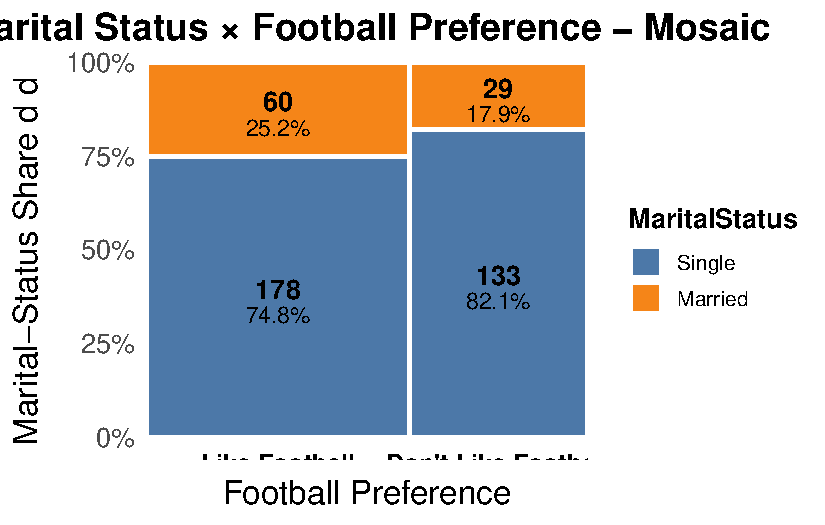
\includegraphics[keepaspectratio]{index_files/figure-pdf/unnamed-chunk-34-1.pdf}}

It represents the proportion of all students who fall into that joint
category (married and do not like football).

The hardest part of working with two-way tables is often deciding which
direction to percentage. Unlike scatterplots---where the explanatory
variable conventionally appears on the x-axis---the layout of a two-way
table is flexible. What matters is not the table's physical orientation
but the conceptual direction of explanation. Percentages must always be
calculated within the explanatory variable's categories.

Consider a few more examples. Suppose we want to know whether
religiosity influences political conservatism. We would likely view
religiosity as the explanatory variable and political orientation as the
response. We would therefore calculate percentages within each
religiosity category (for example, percent conservative among highly
religious, moderately religious, and nonreligious respondents). In
contrast, if we were examining traditional gender roles and gender, we
might hypothesize that gender explains variation in gender-role
attitudes---so gender becomes the explanatory variable, and we would
calculate percentages within columns corresponding to men and women.

In all cases, the rule is consistent: \textbf{percentage within the
explanatory variable}. The physical arrangement of the table---whether
by rows or columns---does not matter, as long as the percentaging
direction aligns with your hypothesis.

\subsection{\texorpdfstring{Another Example of a Two-Way Table: The
\emph{Titanic}}{Another Example of a Two-Way Table: The Titanic}}\label{another-example-of-a-two-way-table-the-titanic}

The sinking of the \emph{Titanic} in 1912 provides a powerful example of
how social class can be associated with survival outcomes. Historical
records suggest that the likelihood of surviving the disaster varied
substantially by passengers' class of service. To explore this
relationship statistically, we can organize the data into a two-way
table that cross-classifies \emph{survival status} (died or survived) by
\emph{class of service} (first, second, third, or crew). This layout
allows us to examine how survival rates differ across social classes and
to consider whether class membership may have influenced the probability
of survival.

\begin{longtable}[]{@{}
  >{\raggedright\arraybackslash}p{(\linewidth - 10\tabcolsep) * \real{0.1667}}
  >{\raggedleft\arraybackslash}p{(\linewidth - 10\tabcolsep) * \real{0.1667}}
  >{\raggedleft\arraybackslash}p{(\linewidth - 10\tabcolsep) * \real{0.1786}}
  >{\raggedleft\arraybackslash}p{(\linewidth - 10\tabcolsep) * \real{0.1786}}
  >{\raggedleft\arraybackslash}p{(\linewidth - 10\tabcolsep) * \real{0.1667}}
  >{\raggedleft\arraybackslash}p{(\linewidth - 10\tabcolsep) * \real{0.1429}}@{}}
\toprule\noalign{}
\begin{minipage}[b]{\linewidth}\raggedright
\textbf{Survival}
\end{minipage} & \begin{minipage}[b]{\linewidth}\raggedleft
\textbf{1: First}
\end{minipage} & \begin{minipage}[b]{\linewidth}\raggedleft
\textbf{2: Second}
\end{minipage} & \begin{minipage}[b]{\linewidth}\raggedleft
\textbf{3: Third}
\end{minipage} & \begin{minipage}[b]{\linewidth}\raggedleft
\textbf{4: Crew}
\end{minipage} & \begin{minipage}[b]{\linewidth}\raggedleft
\textbf{Total}
\end{minipage} \\
\midrule\noalign{}
\endhead
\bottomrule\noalign{}
\endlastfoot
Died & 122 & 167 & 528 & 673 & 1,490 \\
Survived & 203 & 118 & 178 & 212 & 711 \\
\textbf{Total} & \textbf{325} & \textbf{285} & \textbf{706} &
\textbf{885} & \textbf{2,201} \\
\end{longtable}

This table summarizes the fate of all 2,201 people on board, including
the crew. The cross-tabulation structure helps us to see both the raw
frequencies and, later, the conditional percentages that describe
survival likelihood within each class. By calculating percentages within
categories of \emph{class of service}---the explanatory variable---we
can quantify how survival chances differed between first-class
passengers, second-class passengers, those in third class, and members
of the crew. Such tabular organization is foundational in understanding
categorical relationships before progressing to more advanced
inferential techniques.

\subsection{\texorpdfstring{Concept: Univariate, or \emph{Marginal},
Distributions}{Concept: Univariate, or Marginal, Distributions}}\label{concept-univariate-or-marginal-distributions}

Before examining relationships between variables, it is useful to study
each variable individually. The distributions that describe a single
variable---such as \emph{class of service} or \emph{survival}---are
known as \textbf{univariate} or \textbf{marginal} distributions. They
summarize how the total number of observations is divided across the
categories of one variable, without considering any relationship to
other variables.

\subsubsection{\texorpdfstring{Distribution of Passenger \emph{Class of
Service} on the
\emph{Titanic}}{Distribution of Passenger Class of Service on the Titanic}}\label{distribution-of-passenger-class-of-service-on-the-titanic}

\begin{longtable}[]{@{}lrr@{}}
\toprule\noalign{}
\textbf{Class of Service} & \textbf{Frequency} & \textbf{Percent} \\
\midrule\noalign{}
\endhead
\bottomrule\noalign{}
\endlastfoot
1: First & 325 & 14.77 \\
2: Second & 285 & 12.95 \\
3: Third & 706 & 32.08 \\
4: Crew & 885 & 40.21 \\
\textbf{Total} & \textbf{2,201} & \textbf{100.00} \\
\end{longtable}

This table shows the marginal distribution of passenger class.
Approximately 15\% of the people on board traveled in first class, 13\%
in second class, 32\% in third class, and 40\% were crew members. These
percentages describe the composition of everyone on board, regardless of
survival status.

\subsubsection{\texorpdfstring{Distribution of \emph{Survival} After the
Sinking}{Distribution of Survival After the Sinking}}\label{distribution-of-survival-after-the-sinking}

\begin{longtable}[]{@{}lrr@{}}
\toprule\noalign{}
\textbf{Survival Status} & \textbf{Frequency} & \textbf{Percent} \\
\midrule\noalign{}
\endhead
\bottomrule\noalign{}
\endlastfoot
Died & 1,490 & 67.70 \\
Survived & 711 & 32.30 \\
\textbf{Total} & \textbf{2,201} & \textbf{100.00} \\
\end{longtable}

This second table presents the marginal distribution of survival
outcomes. About two-thirds of those on board perished, while
approximately one-third survived. Like the previous table, these values
summarize a single variable and do not yet address how survival may have
depended on other factors such as class of service. Examining these
marginal distributions provides an essential first step before moving to
the joint and conditional analyses that reveal relationships between
variables.

\subsection{Percentages: A Fine Analytical
Tool}\label{percentages-a-fine-analytical-tool}

To examine the relationship between two categorical variables, it is
almost always helpful to express frequencies as percentages---either
across rows or down columns. Percentaging helps us interpret the nature
and strength of associations within a two-way table by revealing
patterns that raw counts may obscure.

Consider again the \emph{Titanic} data. The table below shows the
distribution of survival outcomes by class of service, where the
percentages have been calculated \textbf{down each column}---that is,
\emph{within categories of the explanatory variable} (class of service).

\begin{longtable}[]{@{}
  >{\raggedright\arraybackslash}p{(\linewidth - 10\tabcolsep) * \real{0.1765}}
  >{\raggedleft\arraybackslash}p{(\linewidth - 10\tabcolsep) * \real{0.1647}}
  >{\raggedleft\arraybackslash}p{(\linewidth - 10\tabcolsep) * \real{0.1765}}
  >{\raggedleft\arraybackslash}p{(\linewidth - 10\tabcolsep) * \real{0.1765}}
  >{\raggedleft\arraybackslash}p{(\linewidth - 10\tabcolsep) * \real{0.1647}}
  >{\raggedleft\arraybackslash}p{(\linewidth - 10\tabcolsep) * \real{0.1412}}@{}}
\toprule\noalign{}
\begin{minipage}[b]{\linewidth}\raggedright
\textbf{Survival}
\end{minipage} & \begin{minipage}[b]{\linewidth}\raggedleft
\textbf{1: First}
\end{minipage} & \begin{minipage}[b]{\linewidth}\raggedleft
\textbf{2: Second}
\end{minipage} & \begin{minipage}[b]{\linewidth}\raggedleft
\textbf{3: Third}
\end{minipage} & \begin{minipage}[b]{\linewidth}\raggedleft
\textbf{4: Crew}
\end{minipage} & \begin{minipage}[b]{\linewidth}\raggedleft
\textbf{Total}
\end{minipage} \\
\midrule\noalign{}
\endhead
\bottomrule\noalign{}
\endlastfoot
Died & 122 & 167 & 528 & 673 & 1,490 \\
& (37.54\%) & (58.60\%) & (74.79\%) & (76.05\%) & (67.70\%) \\
Survived & 203 & 118 & 178 & 212 & 711 \\
& (62.46\%) & (41.40\%) & (25.21\%) & (23.95\%) & (32.30\%) \\
\textbf{Total} & \textbf{325} & \textbf{285} & \textbf{706} &
\textbf{885} & \textbf{2,201} \\
& (100\%) & (100\%) & (100\%) & (100\%) & (100\%) \\
\end{longtable}

Here, the rule of thumb is to calculate percentages \textbf{within
categories of the explanatory variable}---in this case, \emph{class of
service}. Each column sums to 100 percent, allowing for direct
comparison across social classes. We can clearly see that passengers in
higher classes had a greater probability of survival: approximately 62\%
of first-class passengers survived, compared to 41\% in second class,
25\% in third class, and 24\% of the crew. Thus, class of service
appears to have been a strong predictor of survival likelihood.

\begin{center}\rule{0.5\linewidth}{0.5pt}\end{center}

\subsection{Percentages in Classes by Survival
Status}\label{percentages-in-classes-by-survival-status}

Sometimes, it is equally informative to percentage the table in the
opposite direction. Instead of asking, ``What percent of each class
survived?'', we might ask, ``Among those who survived, what percent came
from each class?'' This shifts the focus from survival rates
\emph{within} classes to the \emph{composition} of survivors by class.

\begin{longtable}[]{@{}
  >{\raggedright\arraybackslash}p{(\linewidth - 10\tabcolsep) * \real{0.1765}}
  >{\raggedleft\arraybackslash}p{(\linewidth - 10\tabcolsep) * \real{0.1647}}
  >{\raggedleft\arraybackslash}p{(\linewidth - 10\tabcolsep) * \real{0.1765}}
  >{\raggedleft\arraybackslash}p{(\linewidth - 10\tabcolsep) * \real{0.1765}}
  >{\raggedleft\arraybackslash}p{(\linewidth - 10\tabcolsep) * \real{0.1647}}
  >{\raggedleft\arraybackslash}p{(\linewidth - 10\tabcolsep) * \real{0.1412}}@{}}
\toprule\noalign{}
\begin{minipage}[b]{\linewidth}\raggedright
\textbf{Survival}
\end{minipage} & \begin{minipage}[b]{\linewidth}\raggedleft
\textbf{1: First}
\end{minipage} & \begin{minipage}[b]{\linewidth}\raggedleft
\textbf{2: Second}
\end{minipage} & \begin{minipage}[b]{\linewidth}\raggedleft
\textbf{3: Third}
\end{minipage} & \begin{minipage}[b]{\linewidth}\raggedleft
\textbf{4: Crew}
\end{minipage} & \begin{minipage}[b]{\linewidth}\raggedleft
\textbf{Total}
\end{minipage} \\
\midrule\noalign{}
\endhead
\bottomrule\noalign{}
\endlastfoot
Died & 122 & 167 & 528 & 673 & 1,490 \\
& (8.19\%) & (11.21\%) & (35.44\%) & (45.17\%) & (100\%) \\
Survived & 203 & 118 & 178 & 212 & 711 \\
& (28.55\%) & (16.60\%) & (25.04\%) & (29.82\%) & (100\%) \\
\textbf{Total} & \textbf{325} & \textbf{285} & \textbf{706} &
\textbf{885} & \textbf{2,201} \\
& (14.77\%) & (12.95\%) & (32.08\%) & (40.21\%) & (100\%) \\
\end{longtable}

Here, the percentages are calculated \textbf{across rows}, meaning
within categories of \emph{survival status}. The interpretation changes:
among all survivors, about 29\% were crew, 25\% were third-class
passengers, 17\% were second-class passengers, and 29\% were first-class
passengers. Among those who died, nearly half were crew members. This
table highlights differences in \emph{composition} rather than
\emph{likelihood}.

Both perspectives are useful but answer distinct questions. The first
(column percentages) reveals how likely survival was for different
social classes---useful for testing hypotheses about inequality or
privilege. The second (row percentages) reveals how survivors and
victims were distributed across class lines, providing a descriptive
summary of the social makeup of each group.

\begin{center}\rule{0.5\linewidth}{0.5pt}\end{center}

\subsection{Concept: Conditional
Distributions}\label{concept-conditional-distributions}

A two-way table contains multiple types of information, depending on
which parts of it we examine. The \textbf{interior cells} show the
\emph{joint distribution} of two categorical variables---in this case,
\emph{class of service} and \emph{survival}. The \textbf{margins}
display the \emph{marginal distributions} for each variable considered
separately.

\begin{longtable}[]{@{}
  >{\raggedright\arraybackslash}p{(\linewidth - 10\tabcolsep) * \real{0.1765}}
  >{\raggedleft\arraybackslash}p{(\linewidth - 10\tabcolsep) * \real{0.1647}}
  >{\raggedleft\arraybackslash}p{(\linewidth - 10\tabcolsep) * \real{0.1765}}
  >{\raggedleft\arraybackslash}p{(\linewidth - 10\tabcolsep) * \real{0.1765}}
  >{\raggedleft\arraybackslash}p{(\linewidth - 10\tabcolsep) * \real{0.1647}}
  >{\raggedleft\arraybackslash}p{(\linewidth - 10\tabcolsep) * \real{0.1412}}@{}}
\toprule\noalign{}
\begin{minipage}[b]{\linewidth}\raggedright
\textbf{Survival}
\end{minipage} & \begin{minipage}[b]{\linewidth}\raggedleft
\textbf{1: First}
\end{minipage} & \begin{minipage}[b]{\linewidth}\raggedleft
\textbf{2: Second}
\end{minipage} & \begin{minipage}[b]{\linewidth}\raggedleft
\textbf{3: Third}
\end{minipage} & \begin{minipage}[b]{\linewidth}\raggedleft
\textbf{4: Crew}
\end{minipage} & \begin{minipage}[b]{\linewidth}\raggedleft
\textbf{Total}
\end{minipage} \\
\midrule\noalign{}
\endhead
\bottomrule\noalign{}
\endlastfoot
Died & 122 & 167 & 528 & 673 & 1,490 \\
Survived & 203 & 118 & 178 & 212 & 711 \\
\textbf{Total} & \textbf{325} & \textbf{285} & \textbf{706} &
\textbf{885} & \textbf{2,201} \\
\end{longtable}

However, when we isolate a single row or column and calculate
percentages \emph{within} that subset, we obtain a \textbf{conditional
distribution}---that is, the distribution of one variable \emph{given} a
specific value of the other. For instance, the distribution of survival
outcomes \emph{conditional on class of service} shows how survival
varied across classes, while the distribution of classes
\emph{conditional on survival status} reveals the composition of
survivors or victims.

Conditional distributions are the foundation for understanding
relationships between categorical variables. They allow us to assess
whether one variable---such as class of service---is associated with
systematic differences in another---such as survival. The next sections
will explore how to interpret and visualize conditional relationships,
building toward measures of association that quantify the strength of
these patterns.

\subsection{All Six Possible Conditional
Distributions}\label{all-six-possible-conditional-distributions}

In a two-way table with \emph{r} rows and \emph{c} columns, there are (r
+ c) possible conditional distributions. Each distribution represents
one variable's distribution \emph{given} a specific value of the other
variable. For example, in the \emph{Titanic} data, we have four
categories of class and two categories of survival, so (r + c = 4 + 2 =
6) possible conditional distributions.

\begin{longtable}[]{@{}
  >{\raggedright\arraybackslash}p{(\linewidth - 10\tabcolsep) * \real{0.1765}}
  >{\raggedleft\arraybackslash}p{(\linewidth - 10\tabcolsep) * \real{0.1647}}
  >{\raggedleft\arraybackslash}p{(\linewidth - 10\tabcolsep) * \real{0.1765}}
  >{\raggedleft\arraybackslash}p{(\linewidth - 10\tabcolsep) * \real{0.1765}}
  >{\raggedleft\arraybackslash}p{(\linewidth - 10\tabcolsep) * \real{0.1647}}
  >{\raggedleft\arraybackslash}p{(\linewidth - 10\tabcolsep) * \real{0.1412}}@{}}
\toprule\noalign{}
\begin{minipage}[b]{\linewidth}\raggedright
\textbf{Survival}
\end{minipage} & \begin{minipage}[b]{\linewidth}\raggedleft
\textbf{1: First}
\end{minipage} & \begin{minipage}[b]{\linewidth}\raggedleft
\textbf{2: Second}
\end{minipage} & \begin{minipage}[b]{\linewidth}\raggedleft
\textbf{3: Third}
\end{minipage} & \begin{minipage}[b]{\linewidth}\raggedleft
\textbf{4: Crew}
\end{minipage} & \begin{minipage}[b]{\linewidth}\raggedleft
\textbf{Total}
\end{minipage} \\
\midrule\noalign{}
\endhead
\bottomrule\noalign{}
\endlastfoot
Died & 122 & 167 & 528 & 673 & 1,490 \\
Survived & 203 & 118 & 178 & 212 & 711 \\
\textbf{Total} & \textbf{325} & \textbf{285} & \textbf{706} &
\textbf{885} & \textbf{2,201} \\
\end{longtable}

Each row and column of this table can generate a conditional
distribution. For example, the distribution of survival outcomes
\emph{within} each class of service, or the distribution of class
membership \emph{within} each survival category. Altogether, there are
six such conditional distributions available for interpretation.

\begin{center}\rule{0.5\linewidth}{0.5pt}\end{center}

\subsection{Six Possible Conditional Distributions,
Percentaged}\label{six-possible-conditional-distributions-percentaged}

Percentaging the conditional distributions makes the comparison between
groups clearer. The first table below percentages \emph{within columns}
(that is, within each class of service), while the second table
percentages \emph{within rows} (within survival categories).

\begin{longtable}[]{@{}
  >{\raggedright\arraybackslash}p{(\linewidth - 10\tabcolsep) * \real{0.1765}}
  >{\raggedleft\arraybackslash}p{(\linewidth - 10\tabcolsep) * \real{0.1647}}
  >{\raggedleft\arraybackslash}p{(\linewidth - 10\tabcolsep) * \real{0.1765}}
  >{\raggedleft\arraybackslash}p{(\linewidth - 10\tabcolsep) * \real{0.1765}}
  >{\raggedleft\arraybackslash}p{(\linewidth - 10\tabcolsep) * \real{0.1647}}
  >{\raggedleft\arraybackslash}p{(\linewidth - 10\tabcolsep) * \real{0.1412}}@{}}
\toprule\noalign{}
\begin{minipage}[b]{\linewidth}\raggedright
\textbf{Survival}
\end{minipage} & \begin{minipage}[b]{\linewidth}\raggedleft
\textbf{1: First}
\end{minipage} & \begin{minipage}[b]{\linewidth}\raggedleft
\textbf{2: Second}
\end{minipage} & \begin{minipage}[b]{\linewidth}\raggedleft
\textbf{3: Third}
\end{minipage} & \begin{minipage}[b]{\linewidth}\raggedleft
\textbf{4: Crew}
\end{minipage} & \begin{minipage}[b]{\linewidth}\raggedleft
\textbf{Total}
\end{minipage} \\
\midrule\noalign{}
\endhead
\bottomrule\noalign{}
\endlastfoot
Died & 122 (37.54\%) & 167 (58.60\%) & 528 (74.79\%) & 673 (76.05\%) &
1,490 (67.70\%) \\
Survived & 203 (62.46\%) & 118 (41.40\%) & 178 (25.21\%) & 212 (23.95\%)
& 711 (32.30\%) \\
\textbf{Total} & \textbf{325 (100\%)} & \textbf{285 (100\%)} &
\textbf{706 (100\%)} & \textbf{885 (100\%)} & \textbf{2,201 (100\%)} \\
\end{longtable}

The column percentages show that survival chances were much higher for
passengers in the upper classes. Roughly 62\% of first-class passengers
survived, compared to 41\% in second class, 25\% in third class, and
24\% of the crew.

\begin{longtable}[]{@{}
  >{\raggedright\arraybackslash}p{(\linewidth - 10\tabcolsep) * \real{0.1765}}
  >{\raggedleft\arraybackslash}p{(\linewidth - 10\tabcolsep) * \real{0.1647}}
  >{\raggedleft\arraybackslash}p{(\linewidth - 10\tabcolsep) * \real{0.1765}}
  >{\raggedleft\arraybackslash}p{(\linewidth - 10\tabcolsep) * \real{0.1765}}
  >{\raggedleft\arraybackslash}p{(\linewidth - 10\tabcolsep) * \real{0.1647}}
  >{\raggedleft\arraybackslash}p{(\linewidth - 10\tabcolsep) * \real{0.1412}}@{}}
\toprule\noalign{}
\begin{minipage}[b]{\linewidth}\raggedright
\textbf{Survival}
\end{minipage} & \begin{minipage}[b]{\linewidth}\raggedleft
\textbf{1: First}
\end{minipage} & \begin{minipage}[b]{\linewidth}\raggedleft
\textbf{2: Second}
\end{minipage} & \begin{minipage}[b]{\linewidth}\raggedleft
\textbf{3: Third}
\end{minipage} & \begin{minipage}[b]{\linewidth}\raggedleft
\textbf{4: Crew}
\end{minipage} & \begin{minipage}[b]{\linewidth}\raggedleft
\textbf{Total}
\end{minipage} \\
\midrule\noalign{}
\endhead
\bottomrule\noalign{}
\endlastfoot
Died & 122 (8.19\%) & 167 (11.21\%) & 528 (35.44\%) & 673 (45.17\%) &
1,490 (100\%) \\
Survived & 203 (28.55\%) & 118 (16.60\%) & 178 (25.04\%) & 212 (29.82\%)
& 711 (100\%) \\
\textbf{Total} & \textbf{325 (14.77\%)} & \textbf{285 (12.95\%)} &
\textbf{706 (32.08\%)} & \textbf{885 (40.21\%)} & \textbf{2,201
(100\%)} \\
\end{longtable}

By contrast, the row percentages describe the \emph{composition} of
survivors and victims. For example, among those who survived, about 29\%
were first class, 17\% were second class, 25\% were third class, and
30\% were crew. These perspectives complement one another: one focuses
on \emph{likelihoods} (within columns), and the other on
\emph{composition} (within rows).

\begin{center}\rule{0.5\linewidth}{0.5pt}\end{center}

\subsection{Choosing the Direction of
Percentaging}\label{choosing-the-direction-of-percentaging}

A useful rule of thumb guides which direction to percentage:

\begin{quote}
\textbf{If there is an explanatory--response relationship between
variables, calculate percentages \emph{within} each category of the
explanatory variable (and \emph{across} the categories of the
response).}
\end{quote}

In most research applications, the explanatory variable is the one we
think helps \emph{predict} or \emph{explain} differences in the other
variable. For example, class of service likely explains survival, rather
than the reverse. Hence, we percentage within class categories when
studying survival outcomes.

However, in some cases there may be no clear explanatory--response
distinction. In such instances, it can be informative to percentage the
table both ways to obtain complementary insights.

\begin{center}\rule{0.5\linewidth}{0.5pt}\end{center}

\subsection{Associations: Comparing Conditional
Distributions}\label{associations-comparing-conditional-distributions}

Associations between two categorical variables emerge when conditional
distributions differ across groups. These associations can be described
both \emph{qualitatively} and \emph{quantitatively}.

\begin{itemize}
\item
  \textbf{Qualitative description:} identifies the pattern of
  relationship.\\
  Example: ``First-class passengers were more likely to survive than
  third-class passengers.''
\item
  \textbf{Quantitative description:} measures the magnitude of
  difference.\\
  Example: ``The survival rate was 37.25 percentage points higher among
  first-class passengers than among third-class passengers.''
\end{itemize}

To assess an association's strength, we can compute percentage
differences between conditional distributions or compare the numerical
values directly. The greater the difference between conditional
percentages, the stronger the association between variables.

\begin{center}\rule{0.5\linewidth}{0.5pt}\end{center}

\subsection{Example: Admissions by
Race/Ethnicity}\label{example-admissions-by-raceethnicity}

To illustrate, consider a table showing the relationship between
applicants' race/ethnicity and admission outcomes for magnet schools in
Houston.

\begin{longtable}[]{@{}
  >{\raggedright\arraybackslash}p{(\linewidth - 8\tabcolsep) * \real{0.2414}}
  >{\raggedleft\arraybackslash}p{(\linewidth - 8\tabcolsep) * \real{0.1954}}
  >{\raggedleft\arraybackslash}p{(\linewidth - 8\tabcolsep) * \real{0.2299}}
  >{\raggedleft\arraybackslash}p{(\linewidth - 8\tabcolsep) * \real{0.1954}}
  >{\raggedleft\arraybackslash}p{(\linewidth - 8\tabcolsep) * \real{0.1379}}@{}}
\toprule\noalign{}
\begin{minipage}[b]{\linewidth}\raggedright
\textbf{Race/Ethnicity}
\end{minipage} & \begin{minipage}[b]{\linewidth}\raggedleft
\textbf{1: Accepted}
\end{minipage} & \begin{minipage}[b]{\linewidth}\raggedleft
\textbf{2: Wait-listed}
\end{minipage} & \begin{minipage}[b]{\linewidth}\raggedleft
\textbf{3: Rejected}
\end{minipage} & \begin{minipage}[b]{\linewidth}\raggedleft
\textbf{Total}
\end{minipage} \\
\midrule\noalign{}
\endhead
\bottomrule\noalign{}
\endlastfoot
Black/Hispanic & 485 (93.81\%) & 0 (0.00\%) & 32 (6.19\%) & 517
(100\%) \\
Asian & 110 (37.67\%) & 49 (16.78\%) & 133 (45.55\%) & 292 (100\%) \\
White & 336 (35.52\%) & 251 (26.53\%) & 359 (37.95\%) & 946 (100\%) \\
\textbf{Total} & \textbf{931 (53.05\%)} & \textbf{300 (17.09\%)} &
\textbf{524 (29.86\%)} & \textbf{1,755 (100\%)} \\
\end{longtable}

The key to interpreting this table lies in comparing the relevant
conditional distributions---specifically, how the probability of each
admission outcome varies by racial or ethnic group.

\begin{center}\rule{0.5\linewidth}{0.5pt}\end{center}

\subsection{Describing the Marginal
Distributions}\label{describing-the-marginal-distributions}

Begin with a broad, qualitative observation. Among all applicants to the
Houston magnet schools, Black and Hispanic students were most likely to
be accepted, followed by Asian students, and lastly White students.

Next, support the general observation with specific figures.
Approximately 94\% of Black and Hispanic applicants were accepted,
compared to 38\% of Asians and 36\% of Whites. These figures highlight
substantial variation in acceptance rates across racial groups.

\begin{longtable}[]{@{}
  >{\raggedright\arraybackslash}p{(\linewidth - 8\tabcolsep) * \real{0.2414}}
  >{\raggedleft\arraybackslash}p{(\linewidth - 8\tabcolsep) * \real{0.1954}}
  >{\raggedleft\arraybackslash}p{(\linewidth - 8\tabcolsep) * \real{0.2299}}
  >{\raggedleft\arraybackslash}p{(\linewidth - 8\tabcolsep) * \real{0.1954}}
  >{\raggedleft\arraybackslash}p{(\linewidth - 8\tabcolsep) * \real{0.1379}}@{}}
\toprule\noalign{}
\begin{minipage}[b]{\linewidth}\raggedright
\textbf{Race/Ethnicity}
\end{minipage} & \begin{minipage}[b]{\linewidth}\raggedleft
\textbf{1: Accepted}
\end{minipage} & \begin{minipage}[b]{\linewidth}\raggedleft
\textbf{2: Wait-listed}
\end{minipage} & \begin{minipage}[b]{\linewidth}\raggedleft
\textbf{3: Rejected}
\end{minipage} & \begin{minipage}[b]{\linewidth}\raggedleft
\textbf{Total}
\end{minipage} \\
\midrule\noalign{}
\endhead
\bottomrule\noalign{}
\endlastfoot
Black/Hispanic & 485 (93.81\%) & 0 (0.00\%) & 32 (6.19\%) & 517
(100\%) \\
Asian & 110 (37.67\%) & 49 (16.78\%) & 133 (45.55\%) & 292 (100\%) \\
White & 336 (35.52\%) & 251 (26.53\%) & 359 (37.95\%) & 946 (100\%) \\
\textbf{Total} & \textbf{931 (53.05\%)} & \textbf{300 (17.09\%)} &
\textbf{524 (29.86\%)} & \textbf{1,755 (100\%)} \\
\end{longtable}

\begin{center}\rule{0.5\linewidth}{0.5pt}\end{center}

\subsection{Comparing Conditional
Distributions}\label{comparing-conditional-distributions}

We can also identify more nuanced patterns. Whites, for instance, were
more likely to be \emph{wait-listed} than Asians, but slightly less
likely to be outright rejected. Specifically, 27\% of White applicants
were wait-listed and 38\% were rejected, whereas only 17\% of Asian
applicants were wait-listed and 46\% were rejected. Such comparisons
illustrate that even when overall acceptance rates appear similar, the
nature of outcomes may differ significantly between groups.

\begin{longtable}[]{@{}
  >{\raggedright\arraybackslash}p{(\linewidth - 8\tabcolsep) * \real{0.2414}}
  >{\raggedleft\arraybackslash}p{(\linewidth - 8\tabcolsep) * \real{0.1954}}
  >{\raggedleft\arraybackslash}p{(\linewidth - 8\tabcolsep) * \real{0.2299}}
  >{\raggedleft\arraybackslash}p{(\linewidth - 8\tabcolsep) * \real{0.1954}}
  >{\raggedleft\arraybackslash}p{(\linewidth - 8\tabcolsep) * \real{0.1379}}@{}}
\toprule\noalign{}
\begin{minipage}[b]{\linewidth}\raggedright
\textbf{Race/Ethnicity}
\end{minipage} & \begin{minipage}[b]{\linewidth}\raggedleft
\textbf{1: Accepted}
\end{minipage} & \begin{minipage}[b]{\linewidth}\raggedleft
\textbf{2: Wait-listed}
\end{minipage} & \begin{minipage}[b]{\linewidth}\raggedleft
\textbf{3: Rejected}
\end{minipage} & \begin{minipage}[b]{\linewidth}\raggedleft
\textbf{Total}
\end{minipage} \\
\midrule\noalign{}
\endhead
\bottomrule\noalign{}
\endlastfoot
Black/Hispanic & 485 (93.81\%) & 0 (0.00\%) & 32 (6.19\%) & 517
(100\%) \\
Asian & 110 (37.67\%) & 49 (16.78\%) & 133 (45.55\%) & 292 (100\%) \\
White & 336 (35.52\%) & 251 (26.53\%) & 359 (37.95\%) & 946 (100\%) \\
\textbf{Total} & \textbf{931 (53.05\%)} & \textbf{300 (17.09\%)} &
\textbf{524 (29.86\%)} & \textbf{1,755 (100\%)} \\
\end{longtable}

\begin{center}\rule{0.5\linewidth}{0.5pt}\end{center}

\subsection{Summary}\label{summary}

Across these examples, the logic of conditional distributions remains
the same:\\
- \textbf{Marginal distributions} describe one variable at a time.\\
- \textbf{Conditional distributions} describe one variable \emph{given}
the value of another.\\
- Comparing conditional distributions allows us to detect and describe
associations---both qualitatively and quantitatively.

Whether analyzing survival rates on the \emph{Titanic} or admissions by
race, percentaging appropriately and interpreting conditional
relationships carefully are essential steps toward sound sociological
and statistical reasoning.

\subsection{Lurking Variables in Categorical
Tables}\label{lurking-variables-in-categorical-tables}

Just as in regression analysis, the association observed in a two-way
table may be influenced by \textbf{lurking variables}---unobserved or
unmeasured factors that are related to both variables being analyzed.

A lurking variable of importance is typically associated with both the
row and column variables. Because of these associations, changes in the
lurking variable can create apparent relationships between the variables
in the table, even when no direct causal connection exists between them.

Recognizing this possibility reminds us to interpret associations with
caution: sometimes the relationship we observe between two categorical
variables may in fact be driven by a third, unobserved factor.

When we examine a two-way table --- such as gender by voting behavior or
education level by health status --- it is tempting to interpret the
observed association as a direct relationship between the two variables.
Just as in regression analysis, the pattern we see in a contingency
table may in fact be driven by a lurking variable: a third factor that
is not included in the table but is related to both of the variables
that are. Because it shapes both the row and column variables
simultaneously, a lurking variable can create the appearance of a
meaningful association even when no direct causal link exists between
the two variables we are comparing. This possibility is not a technical
nuance but a substantive warning about interpretation. If a lurking
variable is operating behind the scenes, we can easily overstate,
misread, or misattribute the meaning of a cross-tabulated association.
For this reason, responsible analysis requires asking whether an
unmeasured factor could be producing the pattern we see, rather than
assuming that the observed association reflects a direct relationship.
Recognizing lurking variables is a reminder that correlation in a
two-way table does not, by itself, justify causal or substantive
conclusions.

\begin{center}\rule{0.5\linewidth}{0.5pt}\end{center}

\subsection{Example: A Lurking Variable in Medical
Treatments}\label{example-a-lurking-variable-in-medical-treatments}

Consider real data from a medical study comparing two treatments for
kidney stones (Charig, Webb, Payne, and Wickham 1986). The first table
summarizes treatment outcomes without taking into account any additional
information.

\begin{longtable}[]{@{}lrrr@{}}
\toprule\noalign{}
\textbf{Outcome} & \textbf{Treatment A} & \textbf{Treatment B} &
\textbf{Total} \\
\midrule\noalign{}
\endhead
\bottomrule\noalign{}
\endlastfoot
Success & 273 (78\%) & 289 (83\%) & 562 (80\%) \\
Failure & 77 (22\%) & 61 (17\%) & 138 (20\%) \\
\textbf{Total} & \textbf{350 (100\%)} & \textbf{350 (100\%)} &
\textbf{700 (100\%)} \\
\end{longtable}

At first glance, Treatment B appears superior: its success rate is 83
percent compared to 78 percent for Treatment A.\\
However, this comparison ignores an important lurking
variable---\textbf{the size of the kidney stones}---which turns out to
alter the interpretation entirely.

\begin{center}\rule{0.5\linewidth}{0.5pt}\end{center}

\subsection{The Lurking Variable: The Size of the Kidney
Stone}\label{the-lurking-variable-the-size-of-the-kidney-stone}

When the results are broken down by the size of the kidney stones, we
obtain two separate subtables---one for small stones and one for large
stones.\\
Together they sum to the original overall totals but reveal a different
story.

\begin{longtable}[]{@{}
  >{\raggedright\arraybackslash}p{(\linewidth - 10\tabcolsep) * \real{0.1111}}
  >{\raggedleft\arraybackslash}p{(\linewidth - 10\tabcolsep) * \real{0.1984}}
  >{\raggedleft\arraybackslash}p{(\linewidth - 10\tabcolsep) * \real{0.1984}}
  >{\raggedleft\arraybackslash}p{(\linewidth - 10\tabcolsep) * \real{0.1984}}
  >{\raggedleft\arraybackslash}p{(\linewidth - 10\tabcolsep) * \real{0.1984}}
  >{\raggedleft\arraybackslash}p{(\linewidth - 10\tabcolsep) * \real{0.0952}}@{}}
\toprule\noalign{}
\begin{minipage}[b]{\linewidth}\raggedright
\textbf{Outcome}
\end{minipage} & \begin{minipage}[b]{\linewidth}\raggedleft
\textbf{Treatment A (Small)}
\end{minipage} & \begin{minipage}[b]{\linewidth}\raggedleft
\textbf{Treatment B (Small)}
\end{minipage} & \begin{minipage}[b]{\linewidth}\raggedleft
\textbf{Treatment A (Large)}
\end{minipage} & \begin{minipage}[b]{\linewidth}\raggedleft
\textbf{Treatment B (Large)}
\end{minipage} & \begin{minipage}[b]{\linewidth}\raggedleft
\textbf{Total}
\end{minipage} \\
\midrule\noalign{}
\endhead
\bottomrule\noalign{}
\endlastfoot
Success & 81 (93\%) & 234 (87\%) & 192 (73\%) & 55 (69\%) & 562
(80\%) \\
Failure & 6 (7\%) & 36 (13\%) & 71 (27\%) & 25 (31\%) & 138 (20\%) \\
\textbf{Total} & \textbf{87 (100\%)} & \textbf{270 (100\%)} &
\textbf{263 (100\%)} & \textbf{80 (100\%)} & \textbf{700 (100\%)} \\
\end{longtable}

When we compare conditional distributions within each stone-size
category, Treatment A actually performs better than Treatment B for both
small and large stones.\\
Thus, once the lurking variable (stone size) is controlled for, the
apparent advantage of Treatment B disappears---and the conclusion
reverses.

\textbf{Recommendation:} Regardless of stone size, patients fare better
with \textbf{Treatment A}.

\begin{center}\rule{0.5\linewidth}{0.5pt}\end{center}

\subsection{Simpson's Paradox: Marginal vs.~Conditional
Tables}\label{simpsons-paradox-marginal-vs.-conditional-tables}

The above example illustrates \textbf{Simpson's Paradox}, a situation in
which the direction of an association reverses when data are aggregated
versus when they are disaggregated by a third variable.

A three-way table can be viewed as a combination of two (or more)
conditional two-way tables.\\
When we ignore the third variable and combine the subtables, we obtain a
\emph{marginal} two-way table that conceals important variation.

\begin{longtable}[]{@{}
  >{\raggedright\arraybackslash}p{(\linewidth - 4\tabcolsep) * \real{0.5405}}
  >{\raggedright\arraybackslash}p{(\linewidth - 4\tabcolsep) * \real{0.0405}}
  >{\raggedright\arraybackslash}p{(\linewidth - 4\tabcolsep) * \real{0.4189}}@{}}
\toprule\noalign{}
\begin{minipage}[b]{\linewidth}\raggedright
\textbf{Conditional Tables (by Stone Size)}
\end{minipage} & \begin{minipage}[b]{\linewidth}\raggedright
\end{minipage} & \begin{minipage}[b]{\linewidth}\raggedright
\textbf{Marginal Table (Combined)}
\end{minipage} \\
\midrule\noalign{}
\endhead
\bottomrule\noalign{}
\endlastfoot
\textbf{Small Stones} & + & \textbf{Both Sizes} \\
A = 81 Success, 6 Failure & & A = 273 Success, 77 Failure \\
B = 234 Success, 36 Failure & = & B = 289 Success, 61 Failure \\
\textbf{Large Stones} & & \\
A = 192 Success, 71 Failure & & \\
B = 55 Success, 25 Failure & & \\
\end{longtable}

When the direction of association in the marginal table differs from
that in each conditional table, Simpson's Paradox occurs.\\
This paradox highlights the importance of examining associations within
relevant subgroups before drawing conclusions from aggregated data.

\emph{Originally described by Edward H. Simpson (1951).}

\begin{center}\rule{0.5\linewidth}{0.5pt}\end{center}

\subsection{Lurking Variables Short of Simpson's
Paradox}\label{lurking-variables-short-of-simpsons-paradox}

Simpson's Paradox itself is relatively rare, but smaller, subtler
effects of lurking variables are common and often consequential.

Even without a complete reversal, the \textbf{degree of
association}---the magnitude of percentage differences across
categories---can vary substantially once a third variable is
introduced.\\
Examining conditional tables by levels of a third variable helps reveal
how relationships strengthen, weaken, or disappear once that variable is
taken into account.

Thus, differences across conditional tables may qualify or nuance what
appears to be a simple pattern in the aggregated data.\\
As a general principle:\\
\textgreater{} \textbf{Always be mindful of lurking variables.}

\begin{center}\rule{0.5\linewidth}{0.5pt}\end{center}

\subsection{Chapter 5 Highlights}\label{chapter-5-highlights}

A two-way table provides a structured way to display the association (if
any) between two categorical variables.

\begin{itemize}
\tightlist
\item
  The \textbf{interior cells} represent the \textbf{joint distribution}
  of frequencies or proportions across both variables.\\
\item
  The \textbf{margins} display \textbf{marginal distributions}, which
  describe each variable separately.\\
\item
  \textbf{Conditional distributions} show frequencies or proportions of
  one variable \emph{within categories of another}.\\
\item
  Calculating and comparing selected conditional distributions is a
  powerful tool for detecting and interpreting associations between
  categorical variables.
\end{itemize}

Together, these principles form the foundation for understanding how
associations in categorical data can emerge, change, or
disappear---especially in the presence of lurking variables.

\bookmarksetup{startatroot}

\chapter{Chapter 6: Producing Data:
Sampling}\label{chapter-6-producing-data-sampling}

Understanding how data are produced is fundamental to evaluating
empirical claims in the social sciences.\\
\textbf{Sampling}---selecting a subset of cases from a larger
population---enables researchers to draw generalizable conclusions that
would be infeasible or too costly to obtain from a full census.

This chapter introduces core sampling designs, threats to validity, and
(critically) a rigorous, formula-based \textbf{power analysis} so you
can plan a study that is adequately informative. All code is written in
R and is Quarto-ready.

\begin{center}\rule{0.5\linewidth}{0.5pt}\end{center}

\section{Data Collection and Research
Design}\label{data-collection-and-research-design}

\begin{longtable}[]{@{}
  >{\raggedright\arraybackslash}p{(\linewidth - 4\tabcolsep) * \real{0.3333}}
  >{\raggedright\arraybackslash}p{(\linewidth - 4\tabcolsep) * \real{0.3333}}
  >{\raggedright\arraybackslash}p{(\linewidth - 4\tabcolsep) * \real{0.3333}}@{}}
\toprule\noalign{}
\begin{minipage}[b]{\linewidth}\raggedright
\textbf{Type of Design}
\end{minipage} & \begin{minipage}[b]{\linewidth}\raggedright
\textbf{Description}
\end{minipage} & \begin{minipage}[b]{\linewidth}\raggedright
\textbf{Example}
\end{minipage} \\
\midrule\noalign{}
\endhead
\bottomrule\noalign{}
\endlastfoot
\textbf{Observational Study} & Records data without manipulating
conditions. & National survey on political attitudes \\
\textbf{Experimental Study} & Imposes a treatment and measures outcomes.
& Field experiment testing voter mobilization \\
\end{longtable}

Most sociological data originate in \textbf{observational studies},
especially \textbf{sample surveys} designed to describe populations
through representative subsets.

\begin{center}\rule{0.5\linewidth}{0.5pt}\end{center}

\section{Populations, Samples, Parameters, and
Statistics}\label{populations-samples-parameters-and-statistics}

\begin{longtable}[]{@{}
  >{\raggedright\arraybackslash}p{(\linewidth - 4\tabcolsep) * \real{0.3333}}
  >{\raggedright\arraybackslash}p{(\linewidth - 4\tabcolsep) * \real{0.3333}}
  >{\raggedright\arraybackslash}p{(\linewidth - 4\tabcolsep) * \real{0.3333}}@{}}
\toprule\noalign{}
\begin{minipage}[b]{\linewidth}\raggedright
\textbf{Concept}
\end{minipage} & \begin{minipage}[b]{\linewidth}\raggedright
\textbf{Definition}
\end{minipage} & \begin{minipage}[b]{\linewidth}\raggedright
\textbf{Example}
\end{minipage} \\
\midrule\noalign{}
\endhead
\bottomrule\noalign{}
\endlastfoot
\textbf{Population} & The full group of theoretical or empirical
interest. & All working-age people in Wisconsin \\
\textbf{Sample} & The cases actually observed. & 1,000 randomly selected
residents \\
\textbf{Parameter} & A numerical characteristic of the population. &
True mean income \\
\textbf{Statistic} & A numerical characteristic computed from the
sample. & Sample mean income \\
\end{longtable}

A statistic is used to \textbf{estimate} a parameter. Because population
values are typically unknown, our aim is an \textbf{unbiased} and
\textbf{efficient} sample design.

\begin{center}\rule{0.5\linewidth}{0.5pt}\end{center}

\section{Why Use Samples?}\label{why-use-samples}

\begin{itemize}
\tightlist
\item
  A census is often \textbf{too costly} and \textbf{too slow}.\\
\item
  A smaller, well-designed sample can be \textbf{more accurate},
  permitting careful fieldwork and quality control.
\end{itemize}

\begin{center}\rule{0.5\linewidth}{0.5pt}\end{center}

\section{Non-Probability Sampling}\label{non-probability-sampling}

\begin{longtable}[]{@{}
  >{\raggedright\arraybackslash}p{(\linewidth - 4\tabcolsep) * \real{0.3333}}
  >{\raggedright\arraybackslash}p{(\linewidth - 4\tabcolsep) * \real{0.3333}}
  >{\raggedright\arraybackslash}p{(\linewidth - 4\tabcolsep) * \real{0.3333}}@{}}
\toprule\noalign{}
\begin{minipage}[b]{\linewidth}\raggedright
\textbf{Type}
\end{minipage} & \begin{minipage}[b]{\linewidth}\raggedright
\textbf{Description}
\end{minipage} & \begin{minipage}[b]{\linewidth}\raggedright
\textbf{Problem}
\end{minipage} \\
\midrule\noalign{}
\endhead
\bottomrule\noalign{}
\endlastfoot
\textbf{Convenience} & Uses easily available cases. & Over-represents
accessible individuals. \\
\textbf{Voluntary-response} & Participants self-select. & Attracts
highly motivated or extreme respondents. \\
\textbf{Quota} & Interviewers fill demographic quotas non-randomly. &
Vulnerable to interviewer judgment bias. \\
\end{longtable}

\emph{Illustration.} A mail-in poll once found 70\% of parents would not
have children again; a later random sample put that near 7\%. The
voluntary-response design disproportionately selected the disgruntled.

\begin{center}\rule{0.5\linewidth}{0.5pt}\end{center}

\section{Probability Sampling and
Randomization}\label{probability-sampling-and-randomization}

In \textbf{probability sampling}, every individual has a known, nonzero
chance of selection.\\
Randomization limits selection bias by allowing chance---not
judgment---to decide inclusion.

\textbf{Simple Random Sampling (SRS).} Using a complete \textbf{sampling
frame} (a numbered list of population members), draw random numbers to
select cases. Every subset of size (n) is equally likely.

\textbf{Stratified Sampling.} Divide into strata (e.g., gender, region)
and draw an SRS within each stratum. Improves precision and allows
oversampling of smaller but substantively important groups.

\textbf{Multistage Sampling.} Add hierarchical stages (areas → tracts →
households → individuals). Widely used in large surveys (GSS, CPS).
Requires design-based variance estimation and weights.

\begin{center}\rule{0.5\linewidth}{0.5pt}\end{center}

\section{Common Problems in Sampling}\label{common-problems-in-sampling}

\begin{longtable}[]{@{}
  >{\raggedright\arraybackslash}p{(\linewidth - 4\tabcolsep) * \real{0.3333}}
  >{\raggedright\arraybackslash}p{(\linewidth - 4\tabcolsep) * \real{0.3333}}
  >{\raggedright\arraybackslash}p{(\linewidth - 4\tabcolsep) * \real{0.3333}}@{}}
\toprule\noalign{}
\begin{minipage}[b]{\linewidth}\raggedright
\textbf{Problem}
\end{minipage} & \begin{minipage}[b]{\linewidth}\raggedright
\textbf{Definition}
\end{minipage} & \begin{minipage}[b]{\linewidth}\raggedright
\textbf{Example}
\end{minipage} \\
\midrule\noalign{}
\endhead
\bottomrule\noalign{}
\endlastfoot
\textbf{Undercoverage} & Some population members are missing from frame.
& Phone directories omit the phoneless. \\
\textbf{Nonresponse} & Sampled individuals do not participate. &
Refusals or failed contact. \\
\textbf{Response bias} & Misreporting due to sensitivity or recall. &
Income, drug use, voting. \\
\textbf{Wording effects} & Question phrasing influences answers. & ``Do
you agree it is awful that\ldots?'' \\
\textbf{Interviewer effects} & Interviewer traits affect answers. &
Race/gender of interviewer shifts attitudes. \\
\end{longtable}

\begin{center}\rule{0.5\linewidth}{0.5pt}\end{center}

\section{Evaluating Sample Quality}\label{evaluating-sample-quality}

Ask: (1) Is the frame comprehensive? (2) What was the response rate? (3)
Are nonrespondents systematically different? (4) Were protocols unbiased
and consistent?\\
Even random designs can be undermined by poor execution.

\begin{center}\rule{0.5\linewidth}{0.5pt}\end{center}

\section{Power Analysis for Survey Sampling
(Formal)}\label{power-analysis-for-survey-sampling-formal}

Power analysis determines the \textbf{sample size} needed to detect a
substantively meaningful effect with high probability while controlling
Type I error. It formalizes the joint choice of \textbf{effect size},
\textbf{sample size}, \textbf{significance level} (\(\alpha\)), and
\textbf{power} (\(1-\beta\)).

\section{Core quantities}\label{core-quantities}

\begin{longtable}[]{@{}
  >{\centering\arraybackslash}p{(\linewidth - 2\tabcolsep) * \real{0.5714}}
  >{\raggedright\arraybackslash}p{(\linewidth - 2\tabcolsep) * \real{0.4286}}@{}}
\toprule\noalign{}
\begin{minipage}[b]{\linewidth}\centering
\textbf{Symbol}
\end{minipage} & \begin{minipage}[b]{\linewidth}\raggedright
\textbf{Meaning}
\end{minipage} \\
\midrule\noalign{}
\endhead
\bottomrule\noalign{}
\endlastfoot
\(\alpha\) & Type I error (false positive), commonly 0.05 (two-sided
test). \\
\(\beta\) & Type II error (missed detection). \\
\(1-\beta\) & \textbf{Power}: probability of detecting a true effect.
Target 0.80 or 0.90. \\
\(n\) & Sample size (per group, or total, depending on design). \\
\(\Delta\) & Effect size (e.g., difference in proportions or means). \\
\end{longtable}

\section{Two-sample test of proportions (equal group
sizes)}\label{two-sample-test-of-proportions-equal-group-sizes}

Let \(p_0\) be the control proportion and \(p_1\) the treatment
proportion, with effect \(\Delta = p_1 - p_0\). For a two-sided
large-sample \(z\) test:

\begin{itemize}
\item
  Standard error under \(H_1\): \[
  \mathrm{SE} = \sqrt{\frac{p_0(1 - p_0)}{n} + \frac{p_1(1 - p_1)}{n}}.
  \]
\item
  \(z\) statistic under \(H_1\): \(z = \frac{|\Delta|}{\mathrm{SE}}\).
\item
  Required per-group \(n\) for power \(1-\beta\) at level \(\alpha\)
  (approximation): \[
  n \approx \frac{\left[z_{1-\alpha/2}\sqrt{2\bar{p}(1-\bar{p})} + z_{1-\beta}\sqrt{p_0(1-p_0) + p_1(1-p_1)}\right]^2}{(p_1 - p_0)^2}, \qquad \bar{p}=\frac{p_0+p_1}{2}.
  \]
\end{itemize}

\section{\texorpdfstring{Two-sample difference in means (equal group
sizes, pooled SD
\(=\sigma\))}{Two-sample difference in means (equal group sizes, pooled SD =\textbackslash sigma)}}\label{two-sample-difference-in-means-equal-group-sizes-pooled-sd-sigma}

Let \(\Delta = |\mu_1 - \mu_0|\) be the smallest meaningful difference
(in original units). The required \textbf{per-group} sample size is

\[
n \approx 2\left(\frac{(z_{1-\alpha/2} + z_{1-\beta})\sigma}{\Delta}\right)^2
\] Power analysis formulas provide researchers with a systematic method
to determine the minimum sample size required to detect a meaningful
difference between two groups while maintaining specified levels of
statistical confidence. It helps researchers to aim for sufficient
sample size required to achieve their estimation goals. In practice,
researchers typically define the smallest effect size they consider
substantively important, set conventional values for alpha and power,
and then calculate the required sample size. This approach ensures that
studies are neither underpowered (risking to introduce biases into the
analyses) nor wastefully large (consuming unnecessary resources). The
specific formula used depends on the type of data and comparison being
made, with different expressions needed for proportions versus
continuous measurements.

The formula for comparing two proportions addresses situations where we
measure a binary outcome in two groups, such as whether students pass or
fail under different teaching methods, or whether patients recover under
treatment versus control conditions. This formula accounts for the fact
that proportions have a specific variance structure---the variability of
a proportion depends on the proportion itself through the expression
p(1-p), which reaches its maximum at p equals one-half and decreases
toward zero as proportions approach zero or one. The numerator of the
sample size formula contains two components: first, a term involving the
pooled proportion under the null hypothesis (when we assume no
difference exists) multiplied by the critical z-value that corresponds
to our chosen significance level; second, a term that incorporates the
individual group proportions under the alternative hypothesis (when a
true difference exists) multiplied by the z-value corresponding to our
desired power. These two terms represent the sampling distributions
under the null and alternative hypotheses respectively. The denominator
consists of the squared difference between the two proportions---this is
the effect size we wish to detect. When the anticipated difference is
small, the denominator becomes small, which increases the required
sample size substantially. This mathematical relationship captures an
important statistical reality: detecting subtle differences requires
much larger samples than detecting obvious differences.

The formula for comparing two means applies when the outcome variable is
continuous rather than binary, such as test scores, blood pressure
measurements, or income levels. This formula assumes that both groups
have equal sample sizes and share a common standard deviation sigma,
which represents the natural variability in the outcome measure within
each population. The required per-group sample size depends on the ratio
of sigma to delta, where delta represents the smallest meaningful
difference between group means that we consider important to detect.
This ratio, often called the signal-to-noise ratio, captures a
fundamental concept in statistical detection: when measurements are
highly variable (large sigma), we need larger samples to reliably
distinguish a true group difference from random fluctuation. The formula
multiplies this ratio by the sum of two critical values---one
corresponding to the significance level (typically 1.96 for a two-sided
test at alpha equals 0.05) and one corresponding to the desired power
(0.84 for eighty percent power or 1.28 for ninety percent power). The
factor of two in front accounts for the fact that we need this sample
size in each of the two groups being compared. Importantly, this formula
reveals that sample size requirements increase with the square of the
ratio of variability to effect size, meaning that doubling the
variability or halving the effect size requires quadrupling the sample
size to maintain the same statistical power.

\section{Notes for practice}\label{notes-for-practice}

\begin{itemize}
\tightlist
\item
  Use \(z_{1-\alpha/2}=1.96\) for \(\alpha=0.05\) (two-sided) and
  \(z_{1-\beta}=0.84\) or \(1.28\) for target power \(0.80\) or
  \(0.90\), respectively.
\item
  If groups are \textbf{unequal}, replace the per-group \(n\) with
  \(n_0, n_1\) and adjust the standard errors accordingly.
\item
  For \textbf{small samples} or \textbf{binary outcomes with extreme
  \(p\)}, prefer exact or simulation-based power (e.g., via R's
  \texttt{pwr} or \texttt{power.prop.test}).
\end{itemize}

\section{R Setup (Functions, Curves, Tables,
Simulation)}\label{r-setup-functions-curves-tables-simulation}

\begin{Shaded}
\begin{Highlighting}[]
\CommentTok{\# {-}{-}{-}{-} General helpers {-}{-}{-}{-}}
\NormalTok{deff }\OtherTok{\textless{}{-}} \ControlFlowTok{function}\NormalTok{(m, rho) }\DecValTok{1} \SpecialCharTok{+}\NormalTok{ (m }\SpecialCharTok{{-}} \DecValTok{1}\NormalTok{) }\SpecialCharTok{*}\NormalTok{ rho}
\NormalTok{inflate\_n }\OtherTok{\textless{}{-}} \ControlFlowTok{function}\NormalTok{(n\_required, }\AttributeTok{DEFF =} \DecValTok{1}\NormalTok{, }\AttributeTok{drop =} \DecValTok{0}\NormalTok{)\{}
  \FunctionTok{ceiling}\NormalTok{(n\_required }\SpecialCharTok{*}\NormalTok{ DEFF }\SpecialCharTok{/}\NormalTok{ (}\DecValTok{1} \SpecialCharTok{{-}}\NormalTok{ drop))}
\NormalTok{\}}

\CommentTok{\# {-}{-}{-}{-} Two{-}sample proportions {-}{-}{-}{-}}
\NormalTok{power\_prop\_2samp }\OtherTok{\textless{}{-}} \ControlFlowTok{function}\NormalTok{(n\_per\_group, p0, p1, }\AttributeTok{alpha =}\NormalTok{ .}\DecValTok{05}\NormalTok{)\{}
  \CommentTok{\# Normal approx, two{-}sided}
\NormalTok{  q0 }\OtherTok{\textless{}{-}} \DecValTok{1} \SpecialCharTok{{-}}\NormalTok{ p0; q1 }\OtherTok{\textless{}{-}} \DecValTok{1} \SpecialCharTok{{-}}\NormalTok{ p1}
\NormalTok{  se }\OtherTok{\textless{}{-}} \FunctionTok{sqrt}\NormalTok{(p0}\SpecialCharTok{*}\NormalTok{q0}\SpecialCharTok{/}\NormalTok{n\_per\_group }\SpecialCharTok{+}\NormalTok{ p1}\SpecialCharTok{*}\NormalTok{q1}\SpecialCharTok{/}\NormalTok{n\_per\_group)}
\NormalTok{  z  }\OtherTok{\textless{}{-}} \FunctionTok{abs}\NormalTok{(p1 }\SpecialCharTok{{-}}\NormalTok{ p0) }\SpecialCharTok{/}\NormalTok{ se}
\NormalTok{  z\_alpha }\OtherTok{\textless{}{-}} \FunctionTok{qnorm}\NormalTok{(}\DecValTok{1} \SpecialCharTok{{-}}\NormalTok{ alpha}\SpecialCharTok{/}\DecValTok{2}\NormalTok{)}
  \FunctionTok{pnorm}\NormalTok{(z }\SpecialCharTok{{-}}\NormalTok{ z\_alpha) }\SpecialCharTok{+}\NormalTok{ (}\DecValTok{1} \SpecialCharTok{{-}} \FunctionTok{pnorm}\NormalTok{(z }\SpecialCharTok{+}\NormalTok{ z\_alpha))}
\NormalTok{\}}

\NormalTok{n\_prop\_2samp }\OtherTok{\textless{}{-}} \ControlFlowTok{function}\NormalTok{(p0, p1, }\AttributeTok{alpha =}\NormalTok{ .}\DecValTok{05}\NormalTok{, }\AttributeTok{power =}\NormalTok{ .}\DecValTok{80}\NormalTok{)\{}
  \CommentTok{\# Closed{-}form approx (equal n per group)}
\NormalTok{  z\_a }\OtherTok{\textless{}{-}} \FunctionTok{qnorm}\NormalTok{(}\DecValTok{1} \SpecialCharTok{{-}}\NormalTok{ alpha}\SpecialCharTok{/}\DecValTok{2}\NormalTok{)}
\NormalTok{  z\_b }\OtherTok{\textless{}{-}} \FunctionTok{qnorm}\NormalTok{(power)}
\NormalTok{  pbar }\OtherTok{\textless{}{-}}\NormalTok{ (p0 }\SpecialCharTok{+}\NormalTok{ p1)}\SpecialCharTok{/}\DecValTok{2}
\NormalTok{  num }\OtherTok{\textless{}{-}}\NormalTok{ (z\_a}\SpecialCharTok{*}\FunctionTok{sqrt}\NormalTok{(}\DecValTok{2}\SpecialCharTok{*}\NormalTok{pbar}\SpecialCharTok{*}\NormalTok{(}\DecValTok{1} \SpecialCharTok{{-}}\NormalTok{ pbar)) }\SpecialCharTok{+}\NormalTok{ z\_b}\SpecialCharTok{*}\FunctionTok{sqrt}\NormalTok{(p0}\SpecialCharTok{*}\NormalTok{(}\DecValTok{1} \SpecialCharTok{{-}}\NormalTok{ p0) }\SpecialCharTok{+}\NormalTok{ p1}\SpecialCharTok{*}\NormalTok{(}\DecValTok{1} \SpecialCharTok{{-}}\NormalTok{ p1)))}\SpecialCharTok{\^{}}\DecValTok{2}
\NormalTok{  den }\OtherTok{\textless{}{-}}\NormalTok{ (p1 }\SpecialCharTok{{-}}\NormalTok{ p0)}\SpecialCharTok{\^{}}\DecValTok{2}
  \FunctionTok{ceiling}\NormalTok{(num }\SpecialCharTok{/}\NormalTok{ den)}
\NormalTok{\}}

\CommentTok{\# {-}{-}{-}{-} Two{-}sample means {-}{-}{-}{-}}
\NormalTok{power\_mean\_2samp }\OtherTok{\textless{}{-}} \ControlFlowTok{function}\NormalTok{(n\_per\_group, mu0, mu1, sd, }\AttributeTok{alpha =}\NormalTok{ .}\DecValTok{05}\NormalTok{)\{}
\NormalTok{  se }\OtherTok{\textless{}{-}}\NormalTok{ sd }\SpecialCharTok{*} \FunctionTok{sqrt}\NormalTok{(}\DecValTok{2} \SpecialCharTok{/}\NormalTok{ n\_per\_group)}
\NormalTok{  z  }\OtherTok{\textless{}{-}} \FunctionTok{abs}\NormalTok{(mu1 }\SpecialCharTok{{-}}\NormalTok{ mu0) }\SpecialCharTok{/}\NormalTok{ se}
\NormalTok{  z\_alpha }\OtherTok{\textless{}{-}} \FunctionTok{qnorm}\NormalTok{(}\DecValTok{1} \SpecialCharTok{{-}}\NormalTok{ alpha}\SpecialCharTok{/}\DecValTok{2}\NormalTok{)}
  \FunctionTok{pnorm}\NormalTok{(z }\SpecialCharTok{{-}}\NormalTok{ z\_alpha) }\SpecialCharTok{+}\NormalTok{ (}\DecValTok{1} \SpecialCharTok{{-}} \FunctionTok{pnorm}\NormalTok{(z }\SpecialCharTok{+}\NormalTok{ z\_alpha))}
\NormalTok{\}}
\NormalTok{n\_mean\_2samp }\OtherTok{\textless{}{-}} \ControlFlowTok{function}\NormalTok{(delta, sd, }\AttributeTok{alpha =}\NormalTok{ .}\DecValTok{05}\NormalTok{, }\AttributeTok{power =}\NormalTok{ .}\DecValTok{80}\NormalTok{)\{}
\NormalTok{  z\_a }\OtherTok{\textless{}{-}} \FunctionTok{qnorm}\NormalTok{(}\DecValTok{1} \SpecialCharTok{{-}}\NormalTok{ alpha}\SpecialCharTok{/}\DecValTok{2}\NormalTok{)}
\NormalTok{  z\_b }\OtherTok{\textless{}{-}} \FunctionTok{qnorm}\NormalTok{(power)}
\NormalTok{  n }\OtherTok{\textless{}{-}} \DecValTok{2} \SpecialCharTok{*}\NormalTok{ ((z\_a }\SpecialCharTok{+}\NormalTok{ z\_b) }\SpecialCharTok{*}\NormalTok{ sd }\SpecialCharTok{/}\NormalTok{ delta)}\SpecialCharTok{\^{}}\DecValTok{2}
  \FunctionTok{ceiling}\NormalTok{(n)}
\NormalTok{\}}

\CommentTok{\# {-}{-}{-}{-} Regression (partial R\^{}2) {-}{-}{-}{-}}
\NormalTok{n\_reg\_partialR2 }\OtherTok{\textless{}{-}} \ControlFlowTok{function}\NormalTok{(R2\_partial, k, }\AttributeTok{alpha =}\NormalTok{ .}\DecValTok{05}\NormalTok{, }\AttributeTok{power =}\NormalTok{ .}\DecValTok{80}\NormalTok{)\{}
\NormalTok{  f2 }\OtherTok{\textless{}{-}}\NormalTok{ R2\_partial }\SpecialCharTok{/}\NormalTok{ (}\DecValTok{1} \SpecialCharTok{{-}}\NormalTok{ R2\_partial)}
\NormalTok{  Nmax }\OtherTok{\textless{}{-}} \DecValTok{20000}
  \ControlFlowTok{for}\NormalTok{ (n }\ControlFlowTok{in} \FunctionTok{seq}\NormalTok{(k }\SpecialCharTok{+} \DecValTok{5}\NormalTok{, Nmax))\{}
\NormalTok{    df1 }\OtherTok{\textless{}{-}} \DecValTok{1}
\NormalTok{    df2 }\OtherTok{\textless{}{-}}\NormalTok{ n }\SpecialCharTok{{-}}\NormalTok{ (k }\SpecialCharTok{+} \DecValTok{2}\NormalTok{) }\CommentTok{\# intercept + tested + k controls}
    \ControlFlowTok{if}\NormalTok{ (df2 }\SpecialCharTok{\textless{}=} \DecValTok{0}\NormalTok{) }\ControlFlowTok{next}
\NormalTok{    Fcrit }\OtherTok{\textless{}{-}} \FunctionTok{qf}\NormalTok{(}\DecValTok{1} \SpecialCharTok{{-}}\NormalTok{ alpha, df1, df2)}
\NormalTok{    lambda }\OtherTok{\textless{}{-}}\NormalTok{ f2 }\SpecialCharTok{*}\NormalTok{ (df2 }\SpecialCharTok{+} \DecValTok{1}\NormalTok{)}
\NormalTok{    pow }\OtherTok{\textless{}{-}} \DecValTok{1} \SpecialCharTok{{-}} \FunctionTok{pf}\NormalTok{(Fcrit, df1, df2, }\AttributeTok{ncp =}\NormalTok{ lambda)}
    \ControlFlowTok{if}\NormalTok{ (pow }\SpecialCharTok{\textgreater{}=}\NormalTok{ power) }\FunctionTok{return}\NormalTok{(n)}
\NormalTok{  \}}
  \ConstantTok{NA\_integer\_}
\NormalTok{\}}
\end{Highlighting}
\end{Shaded}

\bookmarksetup{startatroot}

\chapter{Chapter 7: Observational vs.~Experimental
Studies}\label{chapter-7-observational-vs.-experimental-studies}

Observational study. We record data on individuals without attempting to
influence them. The investigator does not assign treatments; instead,
observed differences arise from choices, institutions, or circumstances.
Best suited to: describing populations, documenting associations, and
generating hypotheses. Experimental study. We deliberately assign a
treatment (or intervention) to individuals and record their responses.
Random assignment---when feasible---creates groups that are comparable
on average, differing only by treatment. Best suited to: estimating
causal effects under assumptions that are explicit, testable in parts,
and design-driven.

Where Experiments Are Especially Appropriate

Experiments are common in basic psychological research (where mechanisms
are posited to be relatively context-invariant) and in policy evaluation
(where the question is often whether a well-defined program ``works'').
Examples include: Media effects: Do violent video games increase
aggressive behavior? Early childhood programs: Do quality preschools
produce lasting gains in educational attainment or earnings? In such
settings, random assignment can, in principle, equalize (in expectation)
both observed and unobserved characteristics between treatment and
control groups, making the treatment contrast interpretable as causal.

\begin{Shaded}
\begin{Highlighting}[]
\CommentTok{\#| label: tbl{-}design{-}contrast}
\CommentTok{\#| tbl{-}cap: "Contrasting observational and experimental designs."}
\CommentTok{\#| message: false}
\CommentTok{\#| warning: false}

\FunctionTok{library}\NormalTok{(tibble)}
\FunctionTok{library}\NormalTok{(dplyr)}
\FunctionTok{library}\NormalTok{(knitr)}

\NormalTok{contrast }\OtherTok{\textless{}{-}} \FunctionTok{tribble}\NormalTok{(}
  \SpecialCharTok{\textasciitilde{}}\NormalTok{Dimension, }\SpecialCharTok{\textasciitilde{}}\NormalTok{Observational, }\SpecialCharTok{\textasciitilde{}}\NormalTok{Experimental,}
  \StringTok{"Treatment assignment"}\NormalTok{, }\StringTok{"Naturally occurring; not controlled by researcher"}\NormalTok{, }\StringTok{"Assigned by researcher (ideally randomized)"}\NormalTok{,}
  \StringTok{"Primary strength"}\NormalTok{, }\StringTok{"External realism for what people/organizations actually do"}\NormalTok{, }\StringTok{"Internal validity for causal effects"}\NormalTok{,}
  \StringTok{"Primary weakness"}\NormalTok{, }\StringTok{"Confounding from selection \& omitted variables"}\NormalTok{, }\StringTok{"Feasibility, cost, ethics, compliance, spillovers"}\NormalTok{,}
  \StringTok{"Typical estimand"}\NormalTok{, }\StringTok{"Associational contrasts (adjusted or unadjusted)"}\NormalTok{, }\StringTok{"Average treatment effect (ATE/ITT, LATE, etc.)"}\NormalTok{,}
  \StringTok{"Threats"}\NormalTok{, }\StringTok{"Selection bias, omitted variables, reverse causality, measurement error"}\NormalTok{, }\StringTok{"Attrition, non{-}compliance, interference, Hawthorne effects"}\NormalTok{,}
  \StringTok{"Best use"}\NormalTok{, }\StringTok{"Describe patterns; estimate associations; examine heterogeneity"}\NormalTok{, }\StringTok{"Test causal hypotheses; benchmark policy impacts"}
\NormalTok{)}

\FunctionTok{kable}\NormalTok{(contrast, }\AttributeTok{align =} \FunctionTok{c}\NormalTok{(}\StringTok{"l"}\NormalTok{,}\StringTok{"l"}\NormalTok{,}\StringTok{"l"}\NormalTok{))}
\end{Highlighting}
\end{Shaded}

\begin{longtable}[]{@{}
  >{\raggedright\arraybackslash}p{(\linewidth - 4\tabcolsep) * \real{0.1382}}
  >{\raggedright\arraybackslash}p{(\linewidth - 4\tabcolsep) * \real{0.4737}}
  >{\raggedright\arraybackslash}p{(\linewidth - 4\tabcolsep) * \real{0.3882}}@{}}
\toprule\noalign{}
\begin{minipage}[b]{\linewidth}\raggedright
Dimension
\end{minipage} & \begin{minipage}[b]{\linewidth}\raggedright
Observational
\end{minipage} & \begin{minipage}[b]{\linewidth}\raggedright
Experimental
\end{minipage} \\
\midrule\noalign{}
\endhead
\bottomrule\noalign{}
\endlastfoot
Treatment assignment & Naturally occurring; not controlled by researcher
& Assigned by researcher (ideally randomized) \\
Primary strength & External realism for what people/organizations
actually do & Internal validity for causal effects \\
Primary weakness & Confounding from selection \& omitted variables &
Feasibility, cost, ethics, compliance, spillovers \\
Typical estimand & Associational contrasts (adjusted or unadjusted) &
Average treatment effect (ATE/ITT, LATE, etc.) \\
Threats & Selection bias, omitted variables, reverse causality,
measurement error & Attrition, non-compliance, interference, Hawthorne
effects \\
Best use & Describe patterns; estimate associations; examine
heterogeneity & Test causal hypotheses; benchmark policy impacts \\
\end{longtable}

\section{Example: ``Does Preschool Matter in the Long
Run?''}\label{example-does-preschool-matter-in-the-long-run}

Observational approach. Suppose we survey adults about outcomes (e.g.,
earnings) and record whether they attended preschool. A simple
comparison often suggests that preschool attendees do better. But this
contrast may reflect lurking variables---most notably the selection
problem: families who choose (or can access) high-quality preschool
often differ systematically (e.g., in socioeconomic status, parental
education, neighborhood resources), and those differences also predict
adult outcomes. Experimental approach. If we could randomly assign
children to preschool vs.~control (or to quality tiers), then---apart
from chance---both groups would be comparable at baseline. Any
subsequent difference in outcomes would then be attributable to the
program, not to pre-existing family advantages. Randomization thus
targets the confounding that plagues observational comparisons.

\section{Example: ``Does Preschool Matter in the Long
Run?''}\label{example-does-preschool-matter-in-the-long-run-1}

Observational approach. Suppose we survey adults about outcomes (e.g.,
earnings) and record whether they attended preschool. A simple
comparison often suggests that preschool attendees do better. But this
contrast may reflect lurking variables---most notably the selection
problem: families who choose (or can access) high-quality preschool
often differ systematically (e.g., in socioeconomic status, parental
education, neighborhood resources), and those differences also predict
adult outcomes. Experimental approach. If we could randomly assign
children to preschool vs.~control (or to quality tiers), then---apart
from chance---both groups would be comparable at baseline. Any
subsequent difference in outcomes would then be attributable to the
program, not to pre-existing family advantages. Randomization thus
targets the confounding that plagues observational comparisons.

\begin{Shaded}
\begin{Highlighting}[]
\CommentTok{\#| label: fig{-}sim{-}selection{-}and{-}randomization}
\CommentTok{\#| fig{-}cap: ["Selection inflates naive observational effects (synthetic).",}
\CommentTok{\#|           "Randomization recovers the true causal effect (synthetic)."]}
\CommentTok{\#| fig{-}width: 11}
\CommentTok{\#| fig{-}height: 6.5}
\CommentTok{\#| dpi: 300}
\CommentTok{\#| message: false}
\CommentTok{\#| warning: false}

\FunctionTok{suppressPackageStartupMessages}\NormalTok{(\{}
\FunctionTok{library}\NormalTok{(dplyr)}
\FunctionTok{library}\NormalTok{(ggplot2)}
\FunctionTok{library}\NormalTok{(grid)       }\CommentTok{\# for unit(), arrow()}
\NormalTok{\})}

\FunctionTok{set.seed}\NormalTok{(}\DecValTok{123}\NormalTok{)}
\NormalTok{n }\OtherTok{\textless{}{-}} \DecValTok{4000}

\CommentTok{\# Latent family advantage}

\NormalTok{adv }\OtherTok{\textless{}{-}} \FunctionTok{rnorm}\NormalTok{(n, }\DecValTok{0}\NormalTok{, }\DecValTok{1}\NormalTok{)}

\CommentTok{\# True causal effect of preschool on later outcome}

\NormalTok{tau }\OtherTok{\textless{}{-}} \DecValTok{5}

\CommentTok{\# {-}{-}{-}{-}{-}{-}{-}{-}{-}{-}{-}{-}{-}{-}{-}{-}{-}{-}{-}{-}{-}{-}{-}{-}{-}}

\CommentTok{\# OBSERVATIONAL (selection)}

\CommentTok{\# {-}{-}{-}{-}{-}{-}{-}{-}{-}{-}{-}{-}{-}{-}{-}{-}{-}{-}{-}{-}{-}{-}{-}{-}{-}}

\NormalTok{p\_obs }\OtherTok{\textless{}{-}} \FunctionTok{plogis}\NormalTok{(}\SpecialCharTok{{-}}\FloatTok{0.5} \SpecialCharTok{+} \FloatTok{1.0}\SpecialCharTok{*}\NormalTok{adv)}
\NormalTok{D\_obs }\OtherTok{\textless{}{-}} \FunctionTok{rbinom}\NormalTok{(n, }\DecValTok{1}\NormalTok{, p\_obs)}
\NormalTok{y\_obs }\OtherTok{\textless{}{-}} \DecValTok{50} \SpecialCharTok{+} \DecValTok{7}\SpecialCharTok{*}\NormalTok{adv }\SpecialCharTok{+}\NormalTok{ tau}\SpecialCharTok{*}\NormalTok{D\_obs }\SpecialCharTok{+} \FunctionTok{rnorm}\NormalTok{(n, }\DecValTok{0}\NormalTok{, }\DecValTok{8}\NormalTok{)}
\NormalTok{est\_obs }\OtherTok{\textless{}{-}} \FunctionTok{with}\NormalTok{(}\FunctionTok{data.frame}\NormalTok{(}\AttributeTok{D=}\NormalTok{D\_obs, }\AttributeTok{y=}\NormalTok{y\_obs), }\FunctionTok{mean}\NormalTok{(y[D}\SpecialCharTok{==}\DecValTok{1}\NormalTok{]) }\SpecialCharTok{{-}} \FunctionTok{mean}\NormalTok{(y[D}\SpecialCharTok{==}\DecValTok{0}\NormalTok{]))}

\CommentTok{\# {-}{-}{-}{-}{-}{-}{-}{-}{-}{-}{-}{-}{-}{-}{-}}

\CommentTok{\# RANDOMIZED RCT}

\CommentTok{\# {-}{-}{-}{-}{-}{-}{-}{-}{-}{-}{-}{-}{-}{-}{-}}

\NormalTok{D\_rct }\OtherTok{\textless{}{-}} \FunctionTok{rbinom}\NormalTok{(n, }\DecValTok{1}\NormalTok{, }\FloatTok{0.5}\NormalTok{)}
\NormalTok{y\_rct }\OtherTok{\textless{}{-}} \DecValTok{50} \SpecialCharTok{+} \DecValTok{7}\SpecialCharTok{*}\NormalTok{adv }\SpecialCharTok{+}\NormalTok{ tau}\SpecialCharTok{*}\NormalTok{D\_rct }\SpecialCharTok{+} \FunctionTok{rnorm}\NormalTok{(n, }\DecValTok{0}\NormalTok{, }\DecValTok{8}\NormalTok{)}
\NormalTok{est\_rct }\OtherTok{\textless{}{-}} \FunctionTok{with}\NormalTok{(}\FunctionTok{data.frame}\NormalTok{(}\AttributeTok{D=}\NormalTok{D\_rct, }\AttributeTok{y=}\NormalTok{y\_rct), }\FunctionTok{mean}\NormalTok{(y[D}\SpecialCharTok{==}\DecValTok{1}\NormalTok{]) }\SpecialCharTok{{-}} \FunctionTok{mean}\NormalTok{(y[D}\SpecialCharTok{==}\DecValTok{0}\NormalTok{]))}

\CommentTok{\# Palette}

\NormalTok{col\_control        }\OtherTok{\textless{}{-}} \StringTok{"\#FF6B9D"}
\NormalTok{col\_treatment      }\OtherTok{\textless{}{-}} \StringTok{"\#00CED1"}
\NormalTok{col\_control\_dark   }\OtherTok{\textless{}{-}} \StringTok{"\#E63946"}
\NormalTok{col\_treatment\_dark }\OtherTok{\textless{}{-}} \StringTok{"\#0096A8"}

\CommentTok{\# Theme}

\NormalTok{theme\_sexy }\OtherTok{\textless{}{-}} \ControlFlowTok{function}\NormalTok{(}\AttributeTok{base\_size =} \DecValTok{13}\NormalTok{) \{}
\FunctionTok{theme\_minimal}\NormalTok{(}\AttributeTok{base\_size =}\NormalTok{ base\_size, }\AttributeTok{base\_family =} \StringTok{"sans"}\NormalTok{) }\SpecialCharTok{+}
\FunctionTok{theme}\NormalTok{(}
\AttributeTok{panel.grid.major =} \FunctionTok{element\_line}\NormalTok{(}\AttributeTok{color =} \StringTok{"\#F0F0F0"}\NormalTok{, }\AttributeTok{linewidth =} \FloatTok{0.25}\NormalTok{),}
\AttributeTok{panel.grid.minor =} \FunctionTok{element\_blank}\NormalTok{(),}
\AttributeTok{plot.background  =} \FunctionTok{element\_rect}\NormalTok{(}\AttributeTok{fill =} \StringTok{"\#FAFAFA"}\NormalTok{, }\AttributeTok{color =} \ConstantTok{NA}\NormalTok{),}
\AttributeTok{panel.background =} \FunctionTok{element\_rect}\NormalTok{(}\AttributeTok{fill =} \StringTok{"white"}\NormalTok{, }\AttributeTok{color =} \ConstantTok{NA}\NormalTok{),}
\AttributeTok{plot.title       =} \FunctionTok{element\_text}\NormalTok{(}\AttributeTok{face =} \StringTok{"bold"}\NormalTok{, }\AttributeTok{color =} \StringTok{"\#1A1A1A"}\NormalTok{, }\AttributeTok{margin =} \FunctionTok{margin}\NormalTok{(}\AttributeTok{b =} \DecValTok{6}\NormalTok{)),}
\AttributeTok{plot.subtitle    =} \FunctionTok{element\_text}\NormalTok{(}\AttributeTok{color =} \StringTok{"\#666666"}\NormalTok{, }\AttributeTok{margin =} \FunctionTok{margin}\NormalTok{(}\AttributeTok{b =} \DecValTok{10}\NormalTok{)),}
\AttributeTok{axis.title       =} \FunctionTok{element\_text}\NormalTok{(}\AttributeTok{color =} \StringTok{"\#333333"}\NormalTok{, }\AttributeTok{face =} \StringTok{"bold"}\NormalTok{),}
\AttributeTok{axis.text        =} \FunctionTok{element\_text}\NormalTok{(}\AttributeTok{color =} \StringTok{"\#666666"}\NormalTok{),}
\AttributeTok{axis.line        =} \FunctionTok{element\_line}\NormalTok{(}\AttributeTok{color =} \StringTok{"\#CCCCCC"}\NormalTok{, }\AttributeTok{linewidth =} \FloatTok{0.5}\NormalTok{),}
\AttributeTok{axis.ticks       =} \FunctionTok{element\_line}\NormalTok{(}\AttributeTok{color =} \StringTok{"\#CCCCCC"}\NormalTok{, }\AttributeTok{linewidth =} \FloatTok{0.4}\NormalTok{),}
\AttributeTok{axis.ticks.length=} \FunctionTok{unit}\NormalTok{(}\FloatTok{0.12}\NormalTok{, }\StringTok{"cm"}\NormalTok{),}
\AttributeTok{legend.position  =} \StringTok{"top"}\NormalTok{,}
\AttributeTok{legend.justification =} \StringTok{"left"}\NormalTok{,}
\AttributeTok{legend.title     =} \FunctionTok{element\_blank}\NormalTok{(),}
\AttributeTok{legend.text      =} \FunctionTok{element\_text}\NormalTok{(}\AttributeTok{color =} \StringTok{"\#333333"}\NormalTok{),}
\AttributeTok{legend.key.size  =} \FunctionTok{unit}\NormalTok{(}\FloatTok{0.7}\NormalTok{, }\StringTok{"cm"}\NormalTok{),}
\AttributeTok{legend.spacing.x =} \FunctionTok{unit}\NormalTok{(}\FloatTok{0.4}\NormalTok{, }\StringTok{"cm"}\NormalTok{),}
\AttributeTok{legend.margin    =} \FunctionTok{margin}\NormalTok{(}\AttributeTok{b =} \DecValTok{8}\NormalTok{),}
\AttributeTok{legend.background=} \FunctionTok{element\_rect}\NormalTok{(}\AttributeTok{fill =} \StringTok{"white"}\NormalTok{, }\AttributeTok{color =} \ConstantTok{NA}\NormalTok{),}
\AttributeTok{plot.margin      =} \FunctionTok{margin}\NormalTok{(}\DecValTok{15}\NormalTok{, }\DecValTok{20}\NormalTok{, }\DecValTok{10}\NormalTok{, }\DecValTok{15}\NormalTok{)}
\NormalTok{)}
\NormalTok{\}}

\CommentTok{\# {-}{-}{-}{-}{-}{-}{-}{-}}

\CommentTok{\# Plot 1: Observational (selection bias)}

\CommentTok{\# {-}{-}{-}{-}{-}{-}{-}{-}}

\NormalTok{plot\_obs }\OtherTok{\textless{}{-}} \FunctionTok{ggplot}\NormalTok{(}\FunctionTok{data.frame}\NormalTok{(}\AttributeTok{y =}\NormalTok{ y\_obs, }\AttributeTok{D =} \FunctionTok{as.factor}\NormalTok{(D\_obs)),}
\FunctionTok{aes}\NormalTok{(}\AttributeTok{x =}\NormalTok{ y, }\AttributeTok{fill =}\NormalTok{ D, }\AttributeTok{color =}\NormalTok{ D)) }\SpecialCharTok{+}
\FunctionTok{geom\_density}\NormalTok{(}\AttributeTok{alpha =} \FloatTok{0.25}\NormalTok{, }\AttributeTok{linewidth =} \FloatTok{1.5}\NormalTok{, }\AttributeTok{adjust =} \FloatTok{1.2}\NormalTok{) }\SpecialCharTok{+}
\FunctionTok{geom\_density}\NormalTok{(}\AttributeTok{alpha =} \FloatTok{0.15}\NormalTok{, }\AttributeTok{linewidth =} \FloatTok{0.8}\NormalTok{,  }\AttributeTok{adjust =} \FloatTok{1.2}\NormalTok{) }\SpecialCharTok{+}
\FunctionTok{scale\_fill\_manual}\NormalTok{(}\AttributeTok{values =} \FunctionTok{c}\NormalTok{(}\StringTok{"0"} \OtherTok{=}\NormalTok{ col\_control,   }\StringTok{"1"} \OtherTok{=}\NormalTok{ col\_treatment),}
\AttributeTok{labels =} \FunctionTok{c}\NormalTok{(}\StringTok{"Control"}\NormalTok{, }\StringTok{"Preschool"}\NormalTok{)) }\SpecialCharTok{+}
\FunctionTok{scale\_color\_manual}\NormalTok{(}\AttributeTok{values =} \FunctionTok{c}\NormalTok{(}\StringTok{"0"} \OtherTok{=}\NormalTok{ col\_control\_dark, }\StringTok{"1"} \OtherTok{=}\NormalTok{ col\_treatment\_dark),}
\AttributeTok{labels =} \FunctionTok{c}\NormalTok{(}\StringTok{"Control"}\NormalTok{, }\StringTok{"Preschool"}\NormalTok{)) }\SpecialCharTok{+}
\FunctionTok{labs}\NormalTok{(}
\AttributeTok{title    =} \StringTok{"Observational (Selection Bias)"}\NormalTok{,}
\AttributeTok{subtitle =} \FunctionTok{bquote}\NormalTok{(}\FunctionTok{bold}\NormalTok{(}\FunctionTok{hat}\NormalTok{(tau)) }\SpecialCharTok{==} \FunctionTok{bold}\NormalTok{(.(}\FunctionTok{round}\NormalTok{(est\_obs, }\DecValTok{2}\NormalTok{))) }\SpecialCharTok{\textasciitilde{}}
\StringTok{" | true "} \SpecialCharTok{*}\NormalTok{ tau }\SpecialCharTok{==}\NormalTok{ .(tau) }\SpecialCharTok{*} \StringTok{" — inflated by confounding"}\NormalTok{),}
\AttributeTok{x =} \StringTok{"Outcome Score"}\NormalTok{, }\AttributeTok{y =} \StringTok{"Density"}
\NormalTok{) }\SpecialCharTok{+}
\FunctionTok{theme\_sexy}\NormalTok{() }\SpecialCharTok{+}
\FunctionTok{guides}\NormalTok{(}\AttributeTok{fill =} \FunctionTok{guide\_legend}\NormalTok{(}\AttributeTok{override.aes =} \FunctionTok{list}\NormalTok{(}\AttributeTok{alpha =} \FloatTok{0.6}\NormalTok{, }\AttributeTok{linewidth =} \DecValTok{2}\NormalTok{))) }\SpecialCharTok{+}
\FunctionTok{annotate}\NormalTok{(}\StringTok{"segment"}\NormalTok{, }\AttributeTok{x =} \DecValTok{54}\NormalTok{, }\AttributeTok{xend =} \DecValTok{71}\NormalTok{, }\AttributeTok{y =} \FloatTok{0.043}\NormalTok{, }\AttributeTok{yend =} \FloatTok{0.043}\NormalTok{,}
\AttributeTok{color =} \StringTok{"\#E63946"}\NormalTok{, }\AttributeTok{linewidth =} \FloatTok{1.5}\NormalTok{, }\AttributeTok{alpha =} \FloatTok{0.8}\NormalTok{,}
\AttributeTok{arrow =} \FunctionTok{arrow}\NormalTok{(}\AttributeTok{length =} \FunctionTok{unit}\NormalTok{(}\FloatTok{0.25}\NormalTok{, }\StringTok{"cm"}\NormalTok{), }\AttributeTok{type =} \StringTok{"closed"}\NormalTok{)) }\SpecialCharTok{+}
\FunctionTok{annotate}\NormalTok{(}\StringTok{"text"}\NormalTok{, }\AttributeTok{x =} \FloatTok{62.5}\NormalTok{, }\AttributeTok{y =} \FloatTok{0.046}\NormalTok{,}
\AttributeTok{label =} \StringTok{"Spurious difference"}\NormalTok{,}
\AttributeTok{color =} \StringTok{"\#E63946"}\NormalTok{, }\AttributeTok{size =} \FloatTok{3.6}\NormalTok{, }\AttributeTok{fontface =} \StringTok{"bold.italic"}\NormalTok{, }\AttributeTok{alpha =} \FloatTok{0.9}\NormalTok{) }\SpecialCharTok{+}
\FunctionTok{geom\_rug}\NormalTok{(}\FunctionTok{aes}\NormalTok{(}\AttributeTok{color =}\NormalTok{ D), }\AttributeTok{alpha =} \FloatTok{0.02}\NormalTok{, }\AttributeTok{linewidth =} \FloatTok{0.3}\NormalTok{, }\AttributeTok{length =} \FunctionTok{unit}\NormalTok{(}\FloatTok{0.02}\NormalTok{, }\StringTok{"npc"}\NormalTok{))}

\CommentTok{\# {-}{-}{-}{-}{-}{-}{-}{-}}

\CommentTok{\# Plot 2: Randomized (unbiased)}

\CommentTok{\# {-}{-}{-}{-}{-}{-}{-}{-}}

\NormalTok{plot\_rct }\OtherTok{\textless{}{-}} \FunctionTok{ggplot}\NormalTok{(}\FunctionTok{data.frame}\NormalTok{(}\AttributeTok{y =}\NormalTok{ y\_rct, }\AttributeTok{D =} \FunctionTok{as.factor}\NormalTok{(D\_rct)),}
\FunctionTok{aes}\NormalTok{(}\AttributeTok{x =}\NormalTok{ y, }\AttributeTok{fill =}\NormalTok{ D, }\AttributeTok{color =}\NormalTok{ D)) }\SpecialCharTok{+}
\FunctionTok{geom\_density}\NormalTok{(}\AttributeTok{alpha =} \FloatTok{0.25}\NormalTok{, }\AttributeTok{linewidth =} \FloatTok{1.5}\NormalTok{, }\AttributeTok{adjust =} \FloatTok{1.2}\NormalTok{) }\SpecialCharTok{+}
\FunctionTok{geom\_density}\NormalTok{(}\AttributeTok{alpha =} \FloatTok{0.15}\NormalTok{, }\AttributeTok{linewidth =} \FloatTok{0.8}\NormalTok{,  }\AttributeTok{adjust =} \FloatTok{1.2}\NormalTok{) }\SpecialCharTok{+}
\FunctionTok{scale\_fill\_manual}\NormalTok{(}\AttributeTok{values =} \FunctionTok{c}\NormalTok{(}\StringTok{"0"} \OtherTok{=}\NormalTok{ col\_control,   }\StringTok{"1"} \OtherTok{=}\NormalTok{ col\_treatment),}
\AttributeTok{labels =} \FunctionTok{c}\NormalTok{(}\StringTok{"Control"}\NormalTok{, }\StringTok{"Preschool"}\NormalTok{)) }\SpecialCharTok{+}
\FunctionTok{scale\_color\_manual}\NormalTok{(}\AttributeTok{values =} \FunctionTok{c}\NormalTok{(}\StringTok{"0"} \OtherTok{=}\NormalTok{ col\_control\_dark, }\StringTok{"1"} \OtherTok{=}\NormalTok{ col\_treatment\_dark),}
\AttributeTok{labels =} \FunctionTok{c}\NormalTok{(}\StringTok{"Control"}\NormalTok{, }\StringTok{"Preschool"}\NormalTok{)) }\SpecialCharTok{+}
\FunctionTok{labs}\NormalTok{(}
\AttributeTok{title    =} \StringTok{"Randomized (No Selection Bias)"}\NormalTok{,}
\AttributeTok{subtitle =} \FunctionTok{bquote}\NormalTok{(}\FunctionTok{bold}\NormalTok{(}\FunctionTok{hat}\NormalTok{(tau)) }\SpecialCharTok{==} \FunctionTok{bold}\NormalTok{(.(}\FunctionTok{round}\NormalTok{(est\_rct, }\DecValTok{2}\NormalTok{))) }\SpecialCharTok{\textasciitilde{}}
\StringTok{" | true "} \SpecialCharTok{*}\NormalTok{ tau }\SpecialCharTok{==}\NormalTok{ .(tau) }\SpecialCharTok{*} \StringTok{" — unbiased causal estimate"}\NormalTok{),}
\AttributeTok{x =} \StringTok{"Outcome Score"}\NormalTok{, }\AttributeTok{y =} \StringTok{"Density"}
\NormalTok{) }\SpecialCharTok{+}
\FunctionTok{theme\_sexy}\NormalTok{() }\SpecialCharTok{+}
\FunctionTok{guides}\NormalTok{(}\AttributeTok{fill =} \FunctionTok{guide\_legend}\NormalTok{(}\AttributeTok{override.aes =} \FunctionTok{list}\NormalTok{(}\AttributeTok{alpha =} \FloatTok{0.6}\NormalTok{, }\AttributeTok{linewidth =} \DecValTok{2}\NormalTok{))) }\SpecialCharTok{+}
\FunctionTok{annotate}\NormalTok{(}\StringTok{"segment"}\NormalTok{, }\AttributeTok{x =} \DecValTok{47}\NormalTok{, }\AttributeTok{xend =} \DecValTok{57}\NormalTok{, }\AttributeTok{y =} \FloatTok{0.043}\NormalTok{, }\AttributeTok{yend =} \FloatTok{0.043}\NormalTok{,}
\AttributeTok{color =} \StringTok{"\#06D6A0"}\NormalTok{, }\AttributeTok{linewidth =} \FloatTok{1.5}\NormalTok{, }\AttributeTok{alpha =} \FloatTok{0.8}\NormalTok{,}
\AttributeTok{arrow =} \FunctionTok{arrow}\NormalTok{(}\AttributeTok{length =} \FunctionTok{unit}\NormalTok{(}\FloatTok{0.25}\NormalTok{, }\StringTok{"cm"}\NormalTok{), }\AttributeTok{type =} \StringTok{"closed"}\NormalTok{)) }\SpecialCharTok{+}
\FunctionTok{annotate}\NormalTok{(}\StringTok{"text"}\NormalTok{, }\AttributeTok{x =} \DecValTok{52}\NormalTok{, }\AttributeTok{y =} \FloatTok{0.046}\NormalTok{,}
\AttributeTok{label =} \StringTok{"True causal effect"}\NormalTok{,}
\AttributeTok{color =} \StringTok{"\#06D6A0"}\NormalTok{, }\AttributeTok{size =} \FloatTok{3.6}\NormalTok{, }\AttributeTok{fontface =} \StringTok{"bold.italic"}\NormalTok{, }\AttributeTok{alpha =} \FloatTok{0.9}\NormalTok{) }\SpecialCharTok{+}
\FunctionTok{geom\_rug}\NormalTok{(}\FunctionTok{aes}\NormalTok{(}\AttributeTok{color =}\NormalTok{ D), }\AttributeTok{alpha =} \FloatTok{0.02}\NormalTok{, }\AttributeTok{linewidth =} \FloatTok{0.3}\NormalTok{, }\AttributeTok{length =} \FunctionTok{unit}\NormalTok{(}\FloatTok{0.02}\NormalTok{, }\StringTok{"npc"}\NormalTok{))}

\CommentTok{\# {-}{-}{-}{-}{-}}

\CommentTok{\# Print separately (Quarto will emit two large figures)}

\CommentTok{\# {-}{-}{-}{-}{-}}

\NormalTok{plot\_obs}
\end{Highlighting}
\end{Shaded}

\pandocbounded{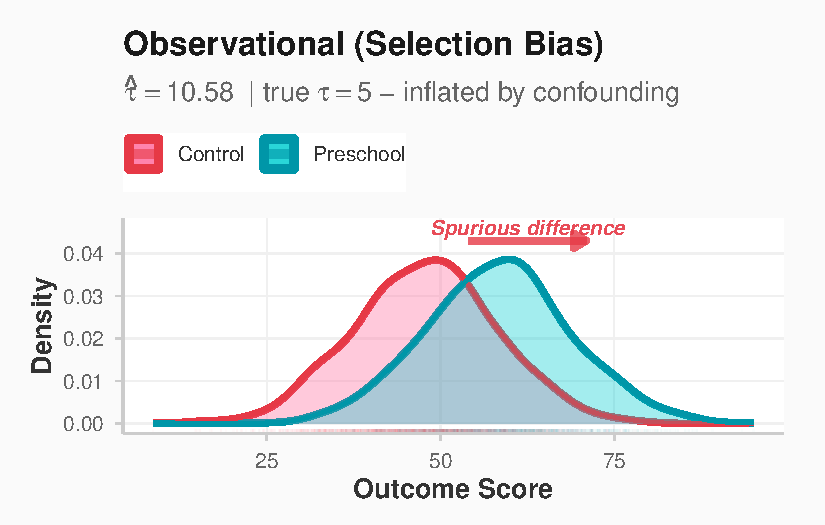
\includegraphics[keepaspectratio]{index_files/figure-pdf/unnamed-chunk-36-1.pdf}}

\begin{Shaded}
\begin{Highlighting}[]
\NormalTok{plot\_rct}
\end{Highlighting}
\end{Shaded}

\pandocbounded{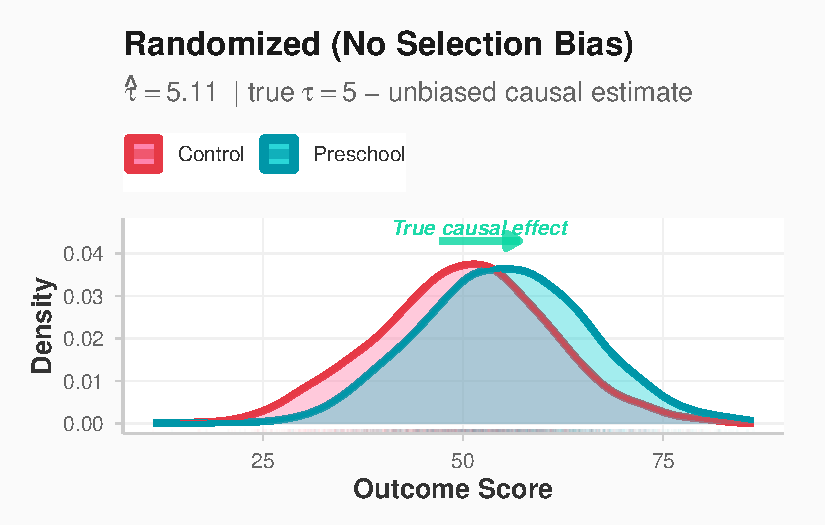
\includegraphics[keepaspectratio]{index_files/figure-pdf/unnamed-chunk-36-2.pdf}}

\section{Experiments in Sociology: A Richer Example than
Preschool}\label{experiments-in-sociology-a-richer-example-than-preschool}

Survey experiments represent a common experimental design to identify
`causal effect' in sociology and political science. In essence, a survey
experiment embeds an experimental treatment---like as a variation in
question wording, framing, or informational content---within a survey
instrument. Survey experiments allow us to identify causal effect
because we are able to randomly assign individuals to a `treatment' and
`control' group. Respondents are randomly assigned to different versions
of the survey, which then allows researchers to assess how specific
manipulations influence attitudes, beliefs, or behaviors. This approach
enables scholars to test theoretical propositions about social and
political processes under controlled conditions while maintaining the
external validity of survey-based research.

Let's look at the following hypothetical examples of `vignette
questions' in survey experiments.

\emph{Eample 1 (Vignette Question 1)}

In Town A, most employers (around 80 \%) pay their employees a living
wage --- enough for a decent standard of living. Almost everyone in the
community (about 90 \%) believes that employers should pay a fair wage,
even if it slightly reduces their profits.

Now imagine Mr.~Hasan Ali, who owns a small local business. One of his
workers has asked for a raise to cover rising food and rent costs.

Question: How likely do you think Mr.~Hasan Ali is to grant the raise
and pay his worker a fair wage?

(1 = Very unlikely \ldots{} 7 = Very likely)

\emph{Example 2 (Vignette Question 2)}

In Town B, most employers (around 80 \%) pay a living wage, but only
about 20 \% believe employers should do so --- most say profit comes
first.

Now imagine Mr.~Hasan Ali, who owns a small local business. One of his
workers has asked for a raise to cover rising food and rent costs.

Question: How likely do you think Mr.~Hasan Ali is to grant the raise
and pay his worker a fair wage?

(1 = Very unlikely \ldots{} 7 = Very likely)

\emph{Results of the Survey Experiment}

The result of the hypothetical survey experiment is interesting: norms
powerfully shape people's predictions about economic outcome, even when
objective circumstances remain constant. In both vignettes, respondents
evaluated the same scenario---Mr.~Hasan Ali, a small business owner
facing a worker's request for a raise to cover rising costs. The
economic reality was identical across conditions: in both Town A and
Town B, approximately 80\% of local employers pay a living wage. Yet
when told that 90\% of the community believed employers should pay fair
wages (the high normative expectation condition), respondents rated
Mr.~Ali as significantly more likely to grant the raise (M = 5.8)
compared to when only 20\% held this belief (the low normative
expectation condition, M = 4.2). This difference of 1.6 points on a
7-point scale---a 38\% increase in perceived likelihood---demonstrates a
very large effect (difference = 1.40) that is both statistically
significant (p \textless{} .001) and practically meaningful.

This finding illuminates how normative climates function as interpretive
frameworks that fundamentally alter our expectations about individual
behavior. Respondents in the high-expectation condition didn't merely
think Mr.~Ali should grant the raise; they genuinely expected he would
do so, even though they knew nothing else about him personally. The
prevailing normative climate---what most people in the community believe
is right---becomes a powerful heuristic for predicting how any given
person will act. When fairness is the shared norm, we anticipate that
individuals will align their behavior accordingly. When
profit-maximization dominates the normative landscape, we become
skeptical that anyone will deviate from self-interest, regardless of
what the actual behavioral data shows. In essence, what a community
collectively values doesn't just influence moral judgments; it shapes
the very reality people expect to encounter in their economic
interactions.

\begin{Shaded}
\begin{Highlighting}[]
\FunctionTok{library}\NormalTok{(ggplot2)}
\FunctionTok{library}\NormalTok{(dplyr)}

\CommentTok{\# 1. Simulate data}
\FunctionTok{set.seed}\NormalTok{(}\DecValTok{123}\NormalTok{)}
\NormalTok{n }\OtherTok{\textless{}{-}} \DecValTok{200}
\NormalTok{data }\OtherTok{\textless{}{-}} \FunctionTok{data.frame}\NormalTok{(}
  \AttributeTok{Condition =} \FunctionTok{rep}\NormalTok{(}\FunctionTok{c}\NormalTok{(}\StringTok{"High Normative Expectation"}\NormalTok{, }\StringTok{"Low Normative Expectation"}\NormalTok{), }\AttributeTok{each =}\NormalTok{ n),}
  \AttributeTok{Score =} \FunctionTok{c}\NormalTok{(}\FunctionTok{rnorm}\NormalTok{(n, }\AttributeTok{mean =} \FloatTok{5.8}\NormalTok{, }\AttributeTok{sd =} \FloatTok{1.1}\NormalTok{), }\FunctionTok{rnorm}\NormalTok{(n, }\AttributeTok{mean =} \FloatTok{4.2}\NormalTok{, }\AttributeTok{sd =} \FloatTok{1.3}\NormalTok{))}
\NormalTok{)}

\CommentTok{\# 2. Calculate summary stats}
\NormalTok{summary\_stats }\OtherTok{\textless{}{-}}\NormalTok{ data }\SpecialCharTok{\%\textgreater{}\%}
  \FunctionTok{group\_by}\NormalTok{(Condition) }\SpecialCharTok{\%\textgreater{}\%}
  \FunctionTok{summarise}\NormalTok{(}
    \AttributeTok{mean =} \FunctionTok{mean}\NormalTok{(Score),}
    \AttributeTok{sd =} \FunctionTok{sd}\NormalTok{(Score),}
    \AttributeTok{se =}\NormalTok{ sd }\SpecialCharTok{/} \FunctionTok{sqrt}\NormalTok{(}\FunctionTok{n}\NormalTok{()),}
    \AttributeTok{ci\_low =}\NormalTok{ mean }\SpecialCharTok{{-}} \FloatTok{1.96} \SpecialCharTok{*}\NormalTok{ se,}
    \AttributeTok{ci\_high =}\NormalTok{ mean }\SpecialCharTok{+} \FloatTok{1.96} \SpecialCharTok{*}\NormalTok{ se}
\NormalTok{  )}

\CommentTok{\# 3. Calculate significance}
\NormalTok{t\_res }\OtherTok{\textless{}{-}} \FunctionTok{t.test}\NormalTok{(Score }\SpecialCharTok{\textasciitilde{}}\NormalTok{ Condition, }\AttributeTok{data =}\NormalTok{ data)}
\NormalTok{p\_val }\OtherTok{\textless{}{-}}\NormalTok{ t\_res}\SpecialCharTok{$}\NormalTok{p.value}
\NormalTok{sig\_label }\OtherTok{\textless{}{-}} \FunctionTok{ifelse}\NormalTok{(p\_val }\SpecialCharTok{\textless{}} \FloatTok{0.001}\NormalTok{, }\StringTok{"***"}\NormalTok{, }
                    \FunctionTok{ifelse}\NormalTok{(p\_val }\SpecialCharTok{\textless{}} \FloatTok{0.01}\NormalTok{, }\StringTok{"**"}\NormalTok{, }
                           \FunctionTok{ifelse}\NormalTok{(p\_val }\SpecialCharTok{\textless{}} \FloatTok{0.05}\NormalTok{, }\StringTok{"*"}\NormalTok{, }\StringTok{"ns"}\NormalTok{)))}

\CommentTok{\# 4. Calculate effect size metrics}
\NormalTok{diff\_means }\OtherTok{\textless{}{-}} \FunctionTok{mean}\NormalTok{(data}\SpecialCharTok{$}\NormalTok{Score[data}\SpecialCharTok{$}\NormalTok{Condition }\SpecialCharTok{==} \StringTok{"High Normative Expectation"}\NormalTok{]) }\SpecialCharTok{{-}} 
              \FunctionTok{mean}\NormalTok{(data}\SpecialCharTok{$}\NormalTok{Score[data}\SpecialCharTok{$}\NormalTok{Condition }\SpecialCharTok{==} \StringTok{"Low Normative Expectation"}\NormalTok{])}

\NormalTok{cohens\_d }\OtherTok{\textless{}{-}}\NormalTok{ diff\_means }\SpecialCharTok{/} \FunctionTok{sd}\NormalTok{(data}\SpecialCharTok{$}\NormalTok{Score)}

 
\FunctionTok{ggplot}\NormalTok{(data, }\FunctionTok{aes}\NormalTok{(}\AttributeTok{x =}\NormalTok{ Condition, }\AttributeTok{y =}\NormalTok{ Score, }\AttributeTok{fill =}\NormalTok{ Condition)) }\SpecialCharTok{+}
  \CommentTok{\# Violin plot}
  \FunctionTok{geom\_violin}\NormalTok{(}
    \AttributeTok{alpha =} \FloatTok{0.8}\NormalTok{,}
    \AttributeTok{trim =} \ConstantTok{FALSE}\NormalTok{,}
    \AttributeTok{scale =} \StringTok{"width"}\NormalTok{,}
    \AttributeTok{color =} \ConstantTok{NA}
\NormalTok{  ) }\SpecialCharTok{+}
  \CommentTok{\# Individual points with jitter}
  \FunctionTok{geom\_jitter}\NormalTok{(}
    \AttributeTok{width =} \FloatTok{0.15}\NormalTok{,}
    \AttributeTok{alpha =} \FloatTok{0.35}\NormalTok{,}
    \AttributeTok{size =} \FloatTok{1.8}\NormalTok{,}
    \AttributeTok{color =} \StringTok{"gray20"}
\NormalTok{  ) }\SpecialCharTok{+}
  \CommentTok{\# Mean with error bars}
  \FunctionTok{geom\_errorbar}\NormalTok{(}
    \AttributeTok{data =}\NormalTok{ summary\_stats,}
    \FunctionTok{aes}\NormalTok{(}\AttributeTok{x =}\NormalTok{ Condition, }\AttributeTok{ymin =}\NormalTok{ ci\_low, }\AttributeTok{ymax =}\NormalTok{ ci\_high),}
    \AttributeTok{width =} \FloatTok{0.15}\NormalTok{,}
    \AttributeTok{linewidth =} \FloatTok{1.3}\NormalTok{,}
    \AttributeTok{color =} \StringTok{"black"}\NormalTok{,}
    \AttributeTok{inherit.aes =} \ConstantTok{FALSE}
\NormalTok{  ) }\SpecialCharTok{+}
  \FunctionTok{geom\_point}\NormalTok{(}
    \AttributeTok{data =}\NormalTok{ summary\_stats,}
    \FunctionTok{aes}\NormalTok{(}\AttributeTok{x =}\NormalTok{ Condition, }\AttributeTok{y =}\NormalTok{ mean),}
    \AttributeTok{size =} \DecValTok{6}\NormalTok{,}
    \AttributeTok{shape =} \DecValTok{21}\NormalTok{,}
    \AttributeTok{fill =} \StringTok{"white"}\NormalTok{,}
    \AttributeTok{color =} \StringTok{"black"}\NormalTok{,}
    \AttributeTok{stroke =} \FloatTok{2.5}\NormalTok{,}
    \AttributeTok{inherit.aes =} \ConstantTok{FALSE}
\NormalTok{  ) }\SpecialCharTok{+}
  \CommentTok{\# Arrow showing difference}
  \FunctionTok{annotate}\NormalTok{(}\StringTok{"segment"}\NormalTok{, }\AttributeTok{x =} \FloatTok{1.2}\NormalTok{, }\AttributeTok{xend =} \FloatTok{1.8}\NormalTok{, }\AttributeTok{y =} \FloatTok{5.2}\NormalTok{, }\AttributeTok{yend =} \FloatTok{5.2}\NormalTok{,}
           \AttributeTok{arrow =} \FunctionTok{arrow}\NormalTok{(}\AttributeTok{length =} \FunctionTok{unit}\NormalTok{(}\FloatTok{0.35}\NormalTok{, }\StringTok{"cm"}\NormalTok{), }\AttributeTok{ends =} \StringTok{"both"}\NormalTok{, }\AttributeTok{type =} \StringTok{"closed"}\NormalTok{),}
           \AttributeTok{linewidth =} \FloatTok{1.2}\NormalTok{, }\AttributeTok{color =} \StringTok{"\#BD3786"}\NormalTok{) }\SpecialCharTok{+}
  \FunctionTok{annotate}\NormalTok{(}\StringTok{"label"}\NormalTok{, }\AttributeTok{x =} \FloatTok{1.5}\NormalTok{, }\AttributeTok{y =} \FloatTok{5.2}\NormalTok{, }
           \AttributeTok{label =} \FunctionTok{sprintf}\NormalTok{(}\StringTok{"Δ = +\%.2f***"}\NormalTok{, diff\_means),}
           \AttributeTok{size =} \FloatTok{4.5}\NormalTok{, }\AttributeTok{fontface =} \StringTok{"bold"}\NormalTok{, }\AttributeTok{fill =} \StringTok{"white"}\NormalTok{, }
           \AttributeTok{label.padding =} \FunctionTok{unit}\NormalTok{(}\FloatTok{0.5}\NormalTok{, }\StringTok{"lines"}\NormalTok{),}
           \AttributeTok{color =} \StringTok{"\#BD3786"}\NormalTok{) }\SpecialCharTok{+}
   \FunctionTok{scale\_fill\_viridis\_d}\NormalTok{(}\AttributeTok{option =} \StringTok{"plasma"}\NormalTok{, }\AttributeTok{begin =} \FloatTok{0.15}\NormalTok{, }\AttributeTok{end =} \FloatTok{0.85}\NormalTok{, }\AttributeTok{direction =} \DecValTok{1}\NormalTok{) }\SpecialCharTok{+}
  \FunctionTok{scale\_x\_discrete}\NormalTok{(}\AttributeTok{labels =} \FunctionTok{c}\NormalTok{(}\StringTok{"High Normative}\SpecialCharTok{\textbackslash{}n}\StringTok{Expectation"}\NormalTok{, }\StringTok{"Low Normative}\SpecialCharTok{\textbackslash{}n}\StringTok{Expectation"}\NormalTok{)) }\SpecialCharTok{+}
  \FunctionTok{labs}\NormalTok{(}
    \AttributeTok{title =} \StringTok{"High Normative Expectations Drive Fairness Perceptions"}\NormalTok{,}
    \AttributeTok{subtitle =} \FunctionTok{sprintf}\NormalTok{(}\StringTok{"Effect size: Cohen\textquotesingle{}s d = \%.2f | 95\%\% CI shown | p \textless{} .001"}\NormalTok{, cohens\_d),}
    \AttributeTok{x =} \StringTok{"Experimental Condition"}\NormalTok{,}
    \AttributeTok{y =} \StringTok{"Perceived Fairness of Raise (1–7 Likert Scale)"}
\NormalTok{  ) }\SpecialCharTok{+}
  \FunctionTok{theme\_minimal}\NormalTok{(}\AttributeTok{base\_size =} \DecValTok{14}\NormalTok{) }\SpecialCharTok{+}
  \FunctionTok{theme}\NormalTok{(}
    \AttributeTok{legend.position =} \StringTok{"none"}\NormalTok{,}
    \AttributeTok{plot.title =} \FunctionTok{element\_text}\NormalTok{(}\AttributeTok{face =} \StringTok{"bold"}\NormalTok{, }\AttributeTok{size =} \DecValTok{17}\NormalTok{, }\AttributeTok{hjust =} \FloatTok{0.5}\NormalTok{, }\AttributeTok{margin =} \FunctionTok{margin}\NormalTok{(}\AttributeTok{b =} \DecValTok{8}\NormalTok{)),}
    \AttributeTok{plot.subtitle =} \FunctionTok{element\_text}\NormalTok{(}\AttributeTok{hjust =} \FloatTok{0.5}\NormalTok{, }\AttributeTok{size =} \DecValTok{11}\NormalTok{, }\AttributeTok{color =} \StringTok{"gray30"}\NormalTok{, }\AttributeTok{margin =} \FunctionTok{margin}\NormalTok{(}\AttributeTok{b =} \DecValTok{15}\NormalTok{)),}
    \AttributeTok{axis.title.x =} \FunctionTok{element\_text}\NormalTok{(}\AttributeTok{face =} \StringTok{"bold"}\NormalTok{, }\AttributeTok{size =} \DecValTok{12}\NormalTok{, }\AttributeTok{margin =} \FunctionTok{margin}\NormalTok{(}\AttributeTok{t =} \DecValTok{10}\NormalTok{)),}
    \AttributeTok{axis.title.y =} \FunctionTok{element\_text}\NormalTok{(}\AttributeTok{face =} \StringTok{"bold"}\NormalTok{, }\AttributeTok{size =} \DecValTok{12}\NormalTok{, }\AttributeTok{margin =} \FunctionTok{margin}\NormalTok{(}\AttributeTok{r =} \DecValTok{10}\NormalTok{)),}
    \AttributeTok{axis.text.x =} \FunctionTok{element\_text}\NormalTok{(}\AttributeTok{size =} \DecValTok{11}\NormalTok{, }\AttributeTok{face =} \StringTok{"bold"}\NormalTok{, }\AttributeTok{lineheight =} \FloatTok{0.9}\NormalTok{),}
    \AttributeTok{axis.text.y =} \FunctionTok{element\_text}\NormalTok{(}\AttributeTok{size =} \DecValTok{11}\NormalTok{),}
    \AttributeTok{panel.grid.major.x =} \FunctionTok{element\_blank}\NormalTok{(),}
    \AttributeTok{panel.grid.minor =} \FunctionTok{element\_blank}\NormalTok{(),}
    \AttributeTok{panel.grid.major.y =} \FunctionTok{element\_line}\NormalTok{(}\AttributeTok{color =} \StringTok{"gray90"}\NormalTok{, }\AttributeTok{linewidth =} \FloatTok{0.5}\NormalTok{),}
    \AttributeTok{plot.background =} \FunctionTok{element\_rect}\NormalTok{(}\AttributeTok{fill =} \StringTok{"white"}\NormalTok{, }\AttributeTok{color =} \ConstantTok{NA}\NormalTok{),}
    \AttributeTok{plot.margin =} \FunctionTok{margin}\NormalTok{(}\DecValTok{20}\NormalTok{, }\DecValTok{20}\NormalTok{, }\DecValTok{20}\NormalTok{, }\DecValTok{20}\NormalTok{)}
\NormalTok{  ) }\SpecialCharTok{+}
  \FunctionTok{coord\_cartesian}\NormalTok{(}\AttributeTok{ylim =} \FunctionTok{c}\NormalTok{(}\DecValTok{1}\NormalTok{, }\DecValTok{7}\NormalTok{))}
\end{Highlighting}
\end{Shaded}

\pandocbounded{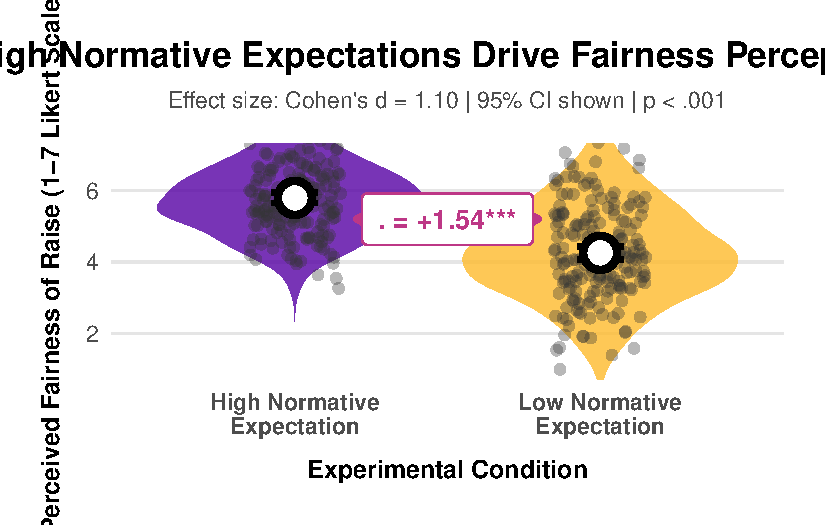
\includegraphics[keepaspectratio]{index_files/figure-pdf/unnamed-chunk-37-1.pdf}}

The growing use of survey experiments reflects a broader methodological
shift toward identifying causal mechanisms in the study of social and
political phenomena. Unlike observational survey data, which can be
limited by issues of confounding and self-selection, the random
assignment inherent in experimental designs allows for stronger claims
about causality. At the same time, because survey experiments are
typically administered to samples that are representative of broader
populations, they preserve many of the advantages of traditional
surveys, such as generalizability and relevance to real-world contexts.
For instance, researchers might test how framing immigration policy in
economic versus humanitarian terms affects public opinion, or how
varying candidate characteristics---such as gender, race, or
ideology---influences voter evaluations.

In the broader social and behavioral sciences, survey experiments are an
essential tool for probing the various dimensions of human judgment and
decision-making. They have been used to explore topics ranging from
racial attitudes and gender bias to the dynamics of political
polarization and trust in institutions. Survey experiments continue to
play a central role in advancing empirical inquiry and deepening our
understanding of the mechanisms that shape public opinion and social
behavior.

When offers are randomized, we can always estimate the
intention-to-treat (ITT): the average outcome difference by offer,
regardless of whether families actually move. If some families do not
use their voucher (non-compliance), ITT is the policy-relevant effect of
the offer. If we also measure who actually moved because of the offer,
we can estimate the treatment-on-the-treated (often called LATE under
standard assumptions): the effect among compliers (families whose moving
decision responds to the offer). Formally:

\textbf{Intention-to-Treat (ITT)} \[
\text{ITT} \;=\; \mathbb{E}[Y \mid Z=1] - \mathbb{E}[Y \mid Z=0],
\] where (Z) is the randomized \textbf{offer} (e.g., E vs.~C), and (Y)
is an outcome.

\textbf{Complier Average Causal Effect (LATE) / Treatment-on-the-Treated
(TOT)} \[
\text{LATE} \;=\; \frac{\mathbb{E}[Y \mid Z=1]-\mathbb{E}[Y \mid Z=0]}
{\mathbb{E}[D \mid Z=1]-\mathbb{E}[D \mid Z=0]}\,,
\] where (D) is \textbf{take-up} (e.g., moved to low-poverty tract).
This is the Wald/IV estimator using (Z) as an instrument for (D).

Interpretation. Randomization equates arms at baseline in expectation;
the observed one-year mean difference is a plausible PT effect, subject
to sampling variation. If a clinically important difference requires ≥6
ODI points, the synthetic trial's 1--3 point advantage would be modest.

\section{Why randomization is powerful (and what it does not
do)}\label{why-randomization-is-powerful-and-what-it-does-not-do}

Randomization ensures that---apart from random noise---the only
systematic difference between groups is the treatment assignment. This
is true even for unmeasured or unmeasurable factors. Randomization does
not guarantee identical groups realized; it guarantees exchangeability
in expectation, which is why we report uncertainty (SEs/CIs) and test
whether differences are too large to be plausibly due to randomization
alone.

\begin{Shaded}
\begin{Highlighting}[]
\FunctionTok{library}\NormalTok{(tibble); }\FunctionTok{library}\NormalTok{(knitr)}
\FunctionTok{tribble}\NormalTok{(}
  \SpecialCharTok{\textasciitilde{}}\NormalTok{Term, }\SpecialCharTok{\textasciitilde{}}\NormalTok{Definition,}
  \StringTok{"Experiment / Trial"}\NormalTok{, }\StringTok{"A design that assigns treatments to units (ideally at random)."}\NormalTok{,}
  \StringTok{"Experimental units"}\NormalTok{, }\StringTok{"The entities assigned (here: families or focal children)."}\NormalTok{,}
  \StringTok{"Subjects / Participants"}\NormalTok{, }\StringTok{"When units are people, we refer to them as subjects/participants."}\NormalTok{,}
  \StringTok{"Factor"}\NormalTok{, }\StringTok{"An explanatory variable manipulated by the researcher (e.g., voucher offer)."}\NormalTok{,}
  \StringTok{"Level"}\NormalTok{, }\StringTok{"A specific setting of a factor (E, S, C)."}\NormalTok{,}
  \StringTok{"Treatment"}\NormalTok{, }\StringTok{"A specific combination of factor levels applied to a unit."}\NormalTok{,}
  \StringTok{"Response (Outcome)"}\NormalTok{, }\StringTok{"A measured result potentially affected by treatment (e.g., test score)."}\NormalTok{,}
  \StringTok{"Compliance"}\NormalTok{, }\StringTok{"Whether units take up the offered treatment (move vs. no move)."}\NormalTok{,}
  \StringTok{"Attrition"}\NormalTok{, }\StringTok{"Loss to follow{-}up; outcomes not observed for some units."}\NormalTok{,}
  \StringTok{"Interference"}\NormalTok{, }\StringTok{"One unit’s treatment affects another’s outcome (spillovers)."}
\NormalTok{) }\SpecialCharTok{|\textgreater{}} 
  \FunctionTok{kable}\NormalTok{(}\AttributeTok{align =} \StringTok{"ll"}\NormalTok{)}
\end{Highlighting}
\end{Shaded}

\begin{longtable}[]{@{}
  >{\raggedright\arraybackslash}p{(\linewidth - 2\tabcolsep) * \real{0.2376}}
  >{\raggedright\arraybackslash}p{(\linewidth - 2\tabcolsep) * \real{0.7624}}@{}}

\caption{\label{tbl-exp-terms}Core experimental terminology in social
research.}

\tabularnewline

\toprule\noalign{}
\begin{minipage}[b]{\linewidth}\raggedright
Term
\end{minipage} & \begin{minipage}[b]{\linewidth}\raggedright
Definition
\end{minipage} \\
\midrule\noalign{}
\endhead
\bottomrule\noalign{}
\endlastfoot
Experiment / Trial & A design that assigns treatments to units (ideally
at random). \\
Experimental units & The entities assigned (here: families or focal
children). \\
Subjects / Participants & When units are people, we refer to them as
subjects/participants. \\
Factor & An explanatory variable manipulated by the researcher (e.g.,
voucher offer). \\
Level & A specific setting of a factor (E, S, C). \\
Treatment & A specific combination of factor levels applied to a
unit. \\
Response (Outcome) & A measured result potentially affected by treatment
(e.g., test score). \\
Compliance & Whether units take up the offered treatment (move vs.~no
move). \\
Attrition & Loss to follow-up; outcomes not observed for some units. \\
Interference & One unit's treatment affects another's outcome
(spillovers). \\

\end{longtable}

\section{When assignment is not randomized: selection
bias}\label{when-assignment-is-not-randomized-selection-bias}

Suppose families with higher parental SES are more successful at
obtaining a coveted preschool slot. If parental SES is positively
related to pre-treatment math aptitude, the treated group will start out
stronger even if the program has zero effect. Post-treatment differences
then confound program impact with pre-existing advantage.

The next setup fabricates a class roster with a latent relationship
between parental SES and math aptitude. We show (i) a non-random
assignment that lets high-SES families select into treatment, then (ii)
a completely randomized assignment.

The goal of this section is to illustrate---using a small synthetic
classroom example---the difference between non-random (selection-based)
assignment and complete randomization, and to show how chance imbalances
naturally arise even under valid randomization.

We begin by constructing an artificial roster of 32 students, each with
a measure of parents' socioeconomic status (SES) and a measure of math
aptitude. The two are deliberately generated to be positively
correlated, mimicking a realistic situation in which students from more
advantaged families tend to score higher. We then simulate two
alternative assignment mechanisms for labeling students as ``treated''
or ``control.'' In the first, the probability of being assigned to
treatment increases with parental SES; this reproduces selection bias:
higher-SES (and thus, on average, higher aptitude) students tend to be
treated. In the second, treatment is assigned by pure coin flip,
enforcing statistical independence between the pre-treatment covariates
and treatment status.

We then summarize pre-treatment math scores by group under each regime
to highlight the consequences of assignment. With selection, the treated
group has a higher mean math aptitude before any intervention; in other
words, group differences pre-exist the treatment. Under complete
randomization, those differences shrink toward zero (up to noise),
because randomization breaks the systematic link between SES/aptitude
and treatment. Finally, to emphasize that randomization controls bias
but not sampling fluctuation, we repeat the random assignment five
independent times and plot the resulting pre-treatment math
distributions. Even when randomization is valid, the realized treated
and control groups may differ more or less from run to run simply by
chance. These five panels illustrate the key logic behind randomization
inference: what matters is not a single realized allocation, but the
distribution of allocations that could have been observed under the same
randomization rule. Together, these code blocks intentionally separate
bias due to selection from variance due to chance---the two fundamental
statistical forces that motivate the use of random assignment and
motivate the need for diagnostics and inference even when randomization
has been correctly carried out.

\begin{Shaded}
\begin{Highlighting}[]
\CommentTok{\#| label: sel{-}vs{-}rand{-}tables}
\CommentTok{\#| tbl{-}cap: "Pre{-}treatment math aptitude by group: non{-}random selection vs. complete randomization (synthetic)."}
\CommentTok{\#| dependson: class{-}setup}
\CommentTok{\#| message: false}
\CommentTok{\#| warning: false}

\FunctionTok{library}\NormalTok{(knitr); }\FunctionTok{library}\NormalTok{(dplyr)}
\NormalTok{summ }\OtherTok{\textless{}{-}} \ControlFlowTok{function}\NormalTok{(df) df }\SpecialCharTok{\%\textgreater{}\%} \FunctionTok{group\_by}\NormalTok{(group) }\SpecialCharTok{\%\textgreater{}\%}
  \FunctionTok{summarise}\NormalTok{(}\AttributeTok{n=}\FunctionTok{n}\NormalTok{(), }\AttributeTok{mean\_mathapt =} \FunctionTok{round}\NormalTok{(}\FunctionTok{mean}\NormalTok{(mathapt),}\DecValTok{1}\NormalTok{),}
            \AttributeTok{sd =} \FunctionTok{round}\NormalTok{(}\FunctionTok{sd}\NormalTok{(mathapt),}\DecValTok{1}\NormalTok{), }\AttributeTok{.groups=}\StringTok{"drop"}\NormalTok{)}

\FunctionTok{kable}\NormalTok{(}\FunctionTok{list}\NormalTok{(}
  \StringTok{\textasciigrave{}}\AttributeTok{Non{-}random selection}\StringTok{\textasciigrave{}} \OtherTok{=} \FunctionTok{summ}\NormalTok{(nr\_alloc),}
  \StringTok{\textasciigrave{}}\AttributeTok{Completely randomized}\StringTok{\textasciigrave{}} \OtherTok{=} \FunctionTok{summ}\NormalTok{(cr\_alloc)}
\NormalTok{), }\AttributeTok{caption =} \ConstantTok{NULL}\NormalTok{)}
\end{Highlighting}
\end{Shaded}

\begin{table}

\centering
\begin{tabular}[t]{l|r|r|r}
\hline
group & n & mean\_mathapt & sd\\
\hline
C & 7 & 41.3 & 6.3\\
\hline
T & 25 & 51.3 & 9.3\\
\hline
\end{tabular}
\centering
\begin{tabular}[t]{l|r|r|r}
\hline
group & n & mean\_mathapt & sd\\
\hline
C & 19 & 48.5 & 8.1\\
\hline
T & 13 & 50.1 & 11.7\\
\hline
\end{tabular}
\end{table}

Under selection, the treatment group begins with a higher mean math
aptitude; under randomization, pre-treatment means are similar (up to
chance). Only the randomized design supports causal interpretation of
the post-treatment contrast.

\section{Completely randomized designs: random variation as a
baseline}\label{completely-randomized-designs-random-variation-as-a-baseline}

Even with randomization, treatment--control differences will vary by
chance across replications. This variation sets the baseline against
which real treatment effects must be compared.

\begin{Shaded}
\begin{Highlighting}[]
\FunctionTok{library}\NormalTok{(dplyr)}
\FunctionTok{library}\NormalTok{(tidyr)}
\FunctionTok{library}\NormalTok{(ggplot2)}

\CommentTok{\# compute run{-}wise Δ(T − C)}

\NormalTok{run\_labels }\OtherTok{\textless{}{-}}\NormalTok{ means\_by\_run }\SpecialCharTok{\%\textgreater{}\%}
\NormalTok{tidyr}\SpecialCharTok{::}\FunctionTok{pivot\_wider}\NormalTok{(}\AttributeTok{names\_from =}\NormalTok{ group, }\AttributeTok{values\_from =}\NormalTok{ mean\_mathapt) }\SpecialCharTok{\%\textgreater{}\%}
\FunctionTok{mutate}\NormalTok{(}
\AttributeTok{run\_num =}\NormalTok{ readr}\SpecialCharTok{::}\FunctionTok{parse\_number}\NormalTok{(run),}
\AttributeTok{delta   =} \StringTok{\textasciigrave{}}\AttributeTok{T}\StringTok{\textasciigrave{}} \SpecialCharTok{{-}}\NormalTok{ C,}
\AttributeTok{lab     =} \FunctionTok{sprintf}\NormalTok{(}\StringTok{"Randomization \%d — Δ(T−C)=\%.1f"}\NormalTok{, run\_num, delta)}
\NormalTok{) }\SpecialCharTok{\%\textgreater{}\%}
\FunctionTok{arrange}\NormalTok{(run\_num) }\SpecialCharTok{\%\textgreater{}\%}
\FunctionTok{select}\NormalTok{(run, lab)}

\CommentTok{\# attach labels to long allocation data}

\NormalTok{allocs\_df\_labeled }\OtherTok{\textless{}{-}}\NormalTok{ allocs\_df }\SpecialCharTok{\%\textgreater{}\%}
\FunctionTok{left\_join}\NormalTok{(run\_labels, }\AttributeTok{by =} \StringTok{"run"}\NormalTok{)}

\FunctionTok{ggplot}\NormalTok{(allocs\_df\_labeled, }\FunctionTok{aes}\NormalTok{(mathapt, }\AttributeTok{fill =}\NormalTok{ group)) }\SpecialCharTok{+}
\FunctionTok{geom\_density}\NormalTok{(}\AttributeTok{alpha =}\NormalTok{ .}\DecValTok{25}\NormalTok{, }\AttributeTok{color =} \ConstantTok{NA}\NormalTok{) }\SpecialCharTok{+}
\FunctionTok{facet\_wrap}\NormalTok{(}\SpecialCharTok{\textasciitilde{}}\NormalTok{ lab, }\AttributeTok{ncol =} \DecValTok{3}\NormalTok{) }\SpecialCharTok{+}
\FunctionTok{scale\_fill\_manual}\NormalTok{(}\AttributeTok{values =} \FunctionTok{c}\NormalTok{(}\AttributeTok{C=}\StringTok{"blue"}\NormalTok{, }\AttributeTok{T=}\StringTok{"yellow"}\NormalTok{),}
\AttributeTok{labels =} \FunctionTok{c}\NormalTok{(}\AttributeTok{C=}\StringTok{"Control"}\NormalTok{, }\AttributeTok{T=}\StringTok{"Treatment"}\NormalTok{)) }\SpecialCharTok{+}
\FunctionTok{labs}\NormalTok{(}
\AttributeTok{title =} \StringTok{"Chance imbalances under valid randomization"}\NormalTok{,}
\AttributeTok{subtitle =} \StringTok{"Each panel is one random allocation; pre{-}treatment T–C gaps (Δ) differ by chance."}\NormalTok{,}
\AttributeTok{x =} \StringTok{"Math aptitude (pre{-}treatment)"}\NormalTok{,}
\AttributeTok{y =} \ConstantTok{NULL}\NormalTok{, }
\AttributeTok{fill =} \ConstantTok{NULL}\NormalTok{, }
\NormalTok{) }\SpecialCharTok{+}
\FunctionTok{theme\_minimal}\NormalTok{(}\AttributeTok{base\_size =} \DecValTok{12}\NormalTok{) }\SpecialCharTok{+}
\FunctionTok{theme}\NormalTok{(}
\AttributeTok{legend.position =} \StringTok{"top"}\NormalTok{,}
\AttributeTok{strip.text      =} \FunctionTok{element\_text}\NormalTok{(}\AttributeTok{face =} \StringTok{"bold"}\NormalTok{),}
\AttributeTok{plot.title      =} \FunctionTok{element\_text}\NormalTok{(}\AttributeTok{face =} \StringTok{"bold"}\NormalTok{),}
\AttributeTok{plot.subtitle   =} \FunctionTok{element\_text}\NormalTok{(}\AttributeTok{margin =} \FunctionTok{margin}\NormalTok{(}\AttributeTok{b =} \DecValTok{6}\NormalTok{))}
\NormalTok{)}
\end{Highlighting}
\end{Shaded}

\begin{figure}[H]

\centering{

\pandocbounded{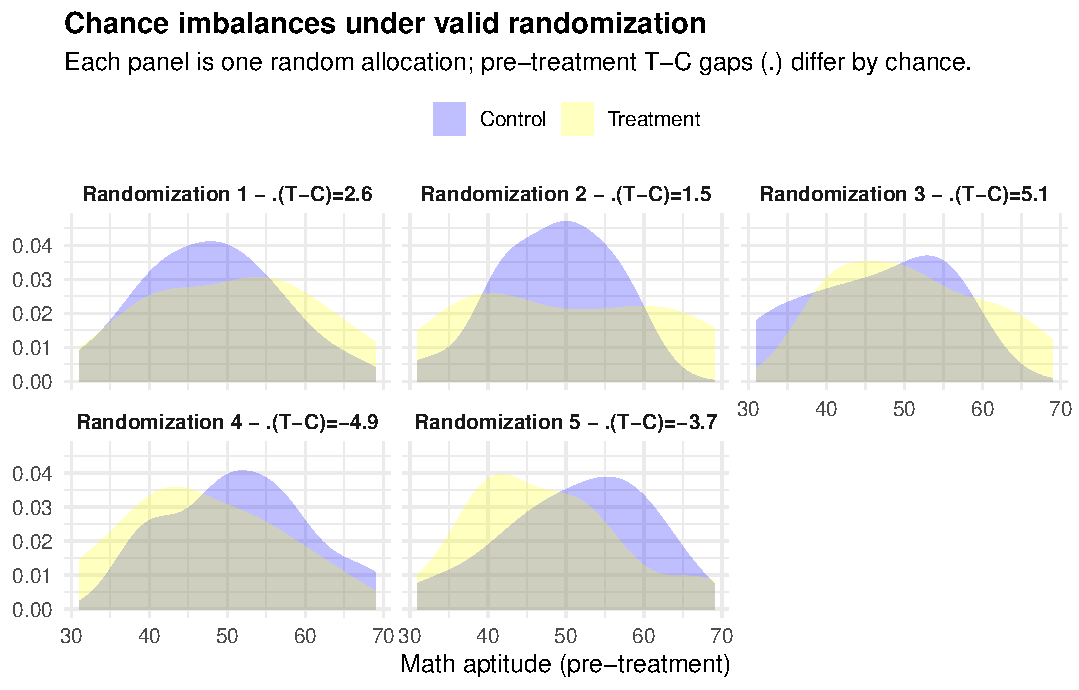
\includegraphics[keepaspectratio]{index_files/figure-pdf/fig-alloc-dists-1.pdf}}

}

\caption{\label{fig-alloc-dists}Five independent completely randomized
allocations. The treatment--control gap in pre-treatment math aptitude
varies by chance.}

\end{figure}%

\begin{Shaded}
\begin{Highlighting}[]
\NormalTok{knitr}\SpecialCharTok{::}\FunctionTok{kable}\NormalTok{(means\_by\_run }\SpecialCharTok{\%\textgreater{}\%}\NormalTok{ tidyr}\SpecialCharTok{::}\FunctionTok{pivot\_wider}\NormalTok{(}\AttributeTok{names\_from =}\NormalTok{ group, }\AttributeTok{values\_from =}\NormalTok{ mean\_mathapt) }\SpecialCharTok{\%\textgreater{}\%}
               \FunctionTok{mutate}\NormalTok{(}\AttributeTok{diff\_T\_minus\_C =} \FunctionTok{round}\NormalTok{(T }\SpecialCharTok{{-}}\NormalTok{ C, }\DecValTok{2}\NormalTok{)),}
             \AttributeTok{align=}\StringTok{"lrrr"}\NormalTok{)}
\end{Highlighting}
\end{Shaded}

\begin{longtable}[]{@{}lrrr@{}}

\caption{\label{tbl-alloc-means}Pre-treatment mean math aptitude by
group across five random allocations (synthetic).}

\tabularnewline

\toprule\noalign{}
run & C & T & diff\_T\_minus\_C \\
\midrule\noalign{}
\endhead
\bottomrule\noalign{}
\endlastfoot
alloc1 & 47.81250 & 50.4375 & 2.62 \\
alloc2 & 48.52632 & 50.0000 & 1.47 \\
alloc3 & 45.91667 & 51.0500 & 5.13 \\
alloc4 & 51.56250 & 46.6875 & -4.88 \\
alloc5 & 51.21429 & 47.5000 & -3.71 \\

\end{longtable}

The figure above shows five different ``coin-flip'' randomizations of
the same classroom into treatment and control. Because the assignment is
random, none of these splits is designed to create a treated group with
higher or lower ability --- but by chance alone, sometimes the treated
students will happen to have slightly higher pre-treatment math scores,
sometimes slightly lower. Each panel reports the observed gap in average
math aptitude before treatment (Δ), and you can see that this Δ is not
the same across runs. The key point is: randomization eliminates
systematic bias, but it does not guarantee perfectly equal groups in
every single draw. Chance imbalances are normal and expected. What
matters is that these imbalances are not caused by selection, but arise
from the same random mechanism we can account for statistically.

Please note that they are all of these randomizations are valid because
they all come from the same fair randomization rule. Some happen to have
a Δ of 5 points, some 1.5, some negative --- but those differences arise
purely by chance, not by design. Randomization does not aim to produce
the smallest imbalance; it aims to produce a comparison whose difference
is not confounded by selection.

If you had to choose one ``best'' by some secondary criterion
(e.g.~smallest imbalance in pre-treatment means), you could pick the run
with Δ closest to zero. But that choice would be post-hoc and would
itself corrupt the logic of random assignment --- you cannot ``pick the
randomization that looks good'' without re-introducing bias.

Takeaway. Randomization equalizes groups on average, not in every
realized sample. Statistical inference quantifies whether a
post-treatment difference is larger than what randomization alone would
plausibly produce.

\section{Design principles (social
experiments)}\label{design-principles-social-experiments}

\begin{enumerate}
\def\labelenumi{\arabic{enumi}.}
\tightlist
\item
  Compare two or more well-defined treatments (often including a
  control).
\item
  Keep everything else as similar as possible across groups.
\item
  Randomize subjects across groups; block or match on key prognostic
  covariates when feasible.
\item
  Use enough units to reduce chance variability; report SEs/CIs.
\item
  Pre-specify estimands and analysis (e.g., ITT, LATE), and report
  compliance, attrition, and spillovers.
\item
  Replicate across samples, sites, and cohorts to assess
  generalizability.
\end{enumerate}

\section{A quick exercise (design
critique)}\label{a-quick-exercise-design-critique}

A winery asks five food-magazine writers to rate its wine,
then---immediately---the competitor's wine; it compares the two ratings.
Problems: tiny and unrepresentative sample; order effects; lack of
blinding; carryover effects; conflict of interest. Better design:
recruit a larger, blinded panel; randomize order of pours within matched
pairs; include replicates; analyze as a matched-pairs experiment with
order as a block.

\section{Summary}\label{summary-1}

Randomized comparative experiments are the most credible basis for
causal inference: by severing the link between potential outcomes and
treatment assignment, they allow outcome differences to be attributed to
the treatment, quantified with uncertainty. When carefully
implemented---using blocks, matching, and transparent estimands---they
remain the gold standard for evaluating interventions in sociology,
policy, and public health.

\bookmarksetup{startatroot}

\chapter{Chapter 8: Probabilities}\label{chapter-8-probabilities}

The notion of probability is central to understanding `statistical
significance.' We are all familiar with expressions like ``there is an
80 percent chance of rain tomorrow,'' meaning the probability is 0.8 and
must fall between 0 and 1. Yet probability is far more than a casual way
of talking about chance---it is a formal branch of mathematics that
provides the foundation for modern statistical reasoning. In social
science research, when our studies are carefully designed, the
mathematical principles of probability become deeply relevant to the
validity and credibility of our findings. Ultimately, it is the way we
conduct our research that determines whether and how probability
calculations can meaningfully inform our conclusions.

The concept of probability has its roots in the work of
seventeenth-century mathematicians who sought to understand games of
chance. Although probability theory continues to underpin gambling and
games of risk, its intellectual significance extends far beyond these
origins. The same mathematical principles that once described dice and
cards later evolved into the foundation of modern statistical
inference---the logic through which researchers draw conclusions about
the world from data. In contemporary research, probability theory
enables us to make valid generalizations from random samples to entire
populations and to assess causal relationships through the controlled
use of randomization in experimental designs.

Probability can be understood as the long-run relative frequency of an
outcome. In essence, when a random process is repeated many times,
patterns begin to emerge that reflect stable underlying probabilities.
This principle allows us to define probability itself: it is the
proportion of times a particular outcome occurs over an indefinitely
large number of trials. For example, while the result of any single coin
toss is inherently unpredictable---assuming the coin is fair---the
relative frequencies of heads and tails become highly consistent over
many tosses. These stable long-run proportions represent the true
probabilities of each possible outcome.

\subsection{Coin toss demonstration (long-run relative
frequency)}\label{coin-toss-demonstration-long-run-relative-frequency}

Calculate the cumulative proportion of heads as you go:

\[
\frac{\text{Total number of heads so far}}{\text{Total number of throws (trials) so far}}
\]

\begin{Shaded}
\begin{Highlighting}[]
\CommentTok{\#| label: fig{-}running{-}proportion{-}pnas}
\CommentTok{\#| fig{-}cap: "Running proportion of heads from a fair coin. Early values wander widely, but the path settles near 0.5 as tosses accumulate."}
\CommentTok{\#| fig{-}width: 7.5}
\CommentTok{\#| fig{-}height: 4.5}
\CommentTok{\#| warning: false}
\CommentTok{\#| message: false}

\FunctionTok{set.seed}\NormalTok{(}\DecValTok{42}\NormalTok{)}
\NormalTok{n }\OtherTok{\textless{}{-}} \DecValTok{800}
\NormalTok{x }\OtherTok{\textless{}{-}} \FunctionTok{rbinom}\NormalTok{(n, }\DecValTok{1}\NormalTok{, }\FloatTok{0.5}\NormalTok{)}
\NormalTok{phat }\OtherTok{\textless{}{-}} \FunctionTok{cumsum}\NormalTok{(x) }\SpecialCharTok{/} \FunctionTok{seq\_len}\NormalTok{(n)}

\FunctionTok{suppressPackageStartupMessages}\NormalTok{(\{}
\FunctionTok{library}\NormalTok{(tibble)}
\FunctionTok{library}\NormalTok{(ggplot2)}

\NormalTok{\})}

\CommentTok{\# PNAS{-}ish minimal theme}

\NormalTok{theme\_pnas }\OtherTok{\textless{}{-}} \ControlFlowTok{function}\NormalTok{(}\AttributeTok{base\_size =} \DecValTok{12}\NormalTok{)\{}
\FunctionTok{theme\_minimal}\NormalTok{(}\AttributeTok{base\_size =}\NormalTok{ base\_size) }\SpecialCharTok{\%+replace\%}
\FunctionTok{theme}\NormalTok{(}
\AttributeTok{plot.title    =} \FunctionTok{element\_text}\NormalTok{(}\AttributeTok{face =} \StringTok{"bold"}\NormalTok{, }\AttributeTok{hjust =} \FloatTok{0.5}\NormalTok{),}
\AttributeTok{plot.subtitle =} \FunctionTok{element\_text}\NormalTok{(}\AttributeTok{margin =} \FunctionTok{margin}\NormalTok{(}\AttributeTok{b =} \DecValTok{8}\NormalTok{), }\AttributeTok{hjust =} \FloatTok{0.5}\NormalTok{),}
\AttributeTok{axis.title.x  =} \FunctionTok{element\_text}\NormalTok{(}\AttributeTok{face =} \StringTok{"bold"}\NormalTok{, }\AttributeTok{margin =} \FunctionTok{margin}\NormalTok{(}\AttributeTok{t =} \DecValTok{6}\NormalTok{)),}
\AttributeTok{axis.title.y  =} \FunctionTok{element\_text}\NormalTok{(}\AttributeTok{face =} \StringTok{"bold"}\NormalTok{, }\AttributeTok{margin =} \FunctionTok{margin}\NormalTok{(}\AttributeTok{r =} \DecValTok{6}\NormalTok{)),}
\AttributeTok{axis.text     =} \FunctionTok{element\_text}\NormalTok{(}\AttributeTok{color =} \StringTok{"gray20"}\NormalTok{),}
\AttributeTok{panel.grid.minor =} \FunctionTok{element\_blank}\NormalTok{(),}
\AttributeTok{panel.grid.major.x =} \FunctionTok{element\_blank}\NormalTok{(),}
\AttributeTok{panel.grid.major.y =} \FunctionTok{element\_line}\NormalTok{(}\AttributeTok{color =} \StringTok{"gray90"}\NormalTok{, }\AttributeTok{linewidth =} \FloatTok{0.5}\NormalTok{),}
\AttributeTok{plot.background   =} \FunctionTok{element\_rect}\NormalTok{(}\AttributeTok{fill =} \StringTok{"white"}\NormalTok{, }\AttributeTok{color =} \ConstantTok{NA}\NormalTok{),}
\AttributeTok{panel.background  =} \FunctionTok{element\_rect}\NormalTok{(}\AttributeTok{fill =} \StringTok{"white"}\NormalTok{, }\AttributeTok{color =} \ConstantTok{NA}\NormalTok{),}
\AttributeTok{legend.position   =} \StringTok{"none"}
\NormalTok{)}
\NormalTok{\}}

\NormalTok{df }\OtherTok{\textless{}{-}} \FunctionTok{tibble}\NormalTok{(}\AttributeTok{t =} \FunctionTok{seq\_len}\NormalTok{(n), }\AttributeTok{phat =}\NormalTok{ phat)}

\FunctionTok{ggplot}\NormalTok{(df, }\FunctionTok{aes}\NormalTok{(}\AttributeTok{x =}\NormalTok{ t, }\AttributeTok{y =}\NormalTok{ phat, }\AttributeTok{color =}\NormalTok{ t)) }\SpecialCharTok{+}
\FunctionTok{geom\_path}\NormalTok{(}\AttributeTok{linewidth =}\NormalTok{ .}\DecValTok{7}\NormalTok{, }\AttributeTok{lineend =} \StringTok{"round"}\NormalTok{) }\SpecialCharTok{+}
\FunctionTok{geom\_hline}\NormalTok{(}\AttributeTok{yintercept =} \FloatTok{0.5}\NormalTok{, }\AttributeTok{linetype =} \StringTok{"dashed"}\NormalTok{, }\AttributeTok{linewidth =} \FloatTok{0.03}\NormalTok{, }\AttributeTok{color =} \StringTok{"gray40"}\NormalTok{) }\SpecialCharTok{+}
\FunctionTok{scale\_color\_viridis\_c}\NormalTok{(}\AttributeTok{option =} \StringTok{"plasma"}\NormalTok{) }\SpecialCharTok{+}
\FunctionTok{scale\_y\_continuous}\NormalTok{(}\AttributeTok{limits =} \FunctionTok{c}\NormalTok{(}\DecValTok{0}\NormalTok{, }\DecValTok{1}\NormalTok{), }\AttributeTok{breaks =} \FunctionTok{seq}\NormalTok{(}\DecValTok{0}\NormalTok{, }\DecValTok{1}\NormalTok{, }\AttributeTok{by =} \FloatTok{0.1}\NormalTok{)) }\SpecialCharTok{+}
\FunctionTok{labs}\NormalTok{(}
\AttributeTok{title    =} \StringTok{"Running Proportion of Heads"}\NormalTok{,}
\AttributeTok{subtitle =} \StringTok{"A fair coin’s running mean converges toward 0.5 (Law of Large Numbers)."}\NormalTok{,}
\AttributeTok{x        =} \StringTok{"Number of tosses (t)"}\NormalTok{,}
\AttributeTok{y        =} \FunctionTok{expression}\NormalTok{(}\FunctionTok{hat}\NormalTok{(p)[t])}
\NormalTok{) }\SpecialCharTok{+}
\FunctionTok{theme\_pnas}\NormalTok{()}
\end{Highlighting}
\end{Shaded}

\pandocbounded{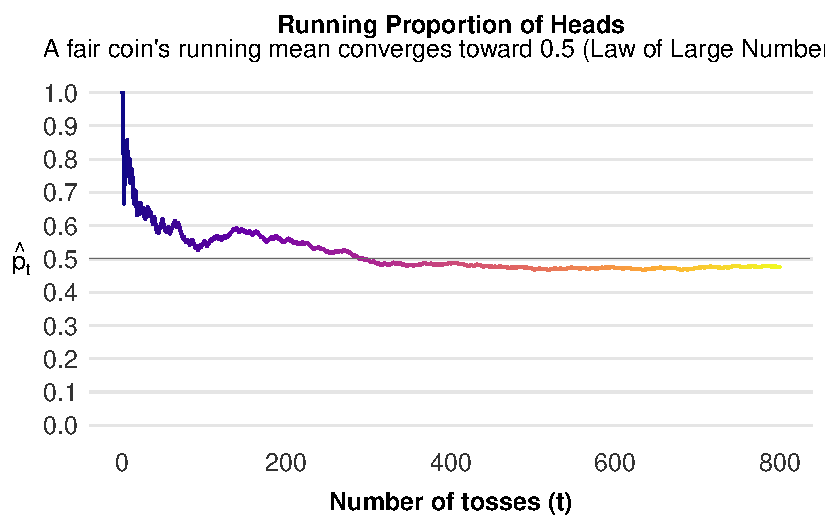
\includegraphics[keepaspectratio]{index_files/figure-pdf/unnamed-chunk-39-1.pdf}}

This simple simulation vividly demonstrates one of the most foundational
ideas in probability and statistics---the law of large numbers. Each
coin toss is inherently random: any single outcome offers no information
about the next, and short sequences often fluctuate dramatically.
However, as the number of tosses accumulates, these random ups and downs
begin to balance out. The running proportion of heads, which initially
swings erratically, gradually stabilizes near 0.5---the true probability
for a fair coin. What we are witnessing is the convergence of the
empirical or observed probability toward the theoretical probability.
This convergence illustrates how randomness behaves in aggregate: while
individual events remain unpredictable, the overall pattern becomes
highly regular when trials are repeated many times. The figure thus
offers a visual intuition for why sample averages and proportions form
the cornerstone of statistical inference---because with enough
observations, random variation cancels out, revealing the stable,
underlying probability structure that governs the process.

Every probability model has two essential components: \textbf{(1)} a
\emph{sample space}, denoted \textbackslash(S\textbackslash), which
lists all possible outcomes of an experiment, and \textbf{(2)} a
\emph{probability assignment} that specifies the likelihood of each
event within that space.

A sample space:

\[
S = \\{\\text{Head},\\ \\text{Tail}\\}
\]

Probability of each outcome in the sample space:

\[
\\Pr(\\text{Head}) = 0.5
\]

\[
\\Pr(\\text{Tail}) = 0.5
\]

A probability model for a \emph{series} of coin flips is made up of
separate models for single flips, combined in a particular way. ``)

\subsection{Defining a sample space: the free-throw
shooter}\label{defining-a-sample-space-the-free-throw-shooter}

To define a probability model, we must first specify the \textbf{sample
space}---the set of all possible outcomes of the random process we are
studying.\\
Consider observing a basketball player taking three free throws. What
should our sample space be?

If we are only interested in the \emph{number} of successful shots, a
simple and sufficient sample space is

{[} S = \{0, 1, 2, 3\}, {]}

where each element represents the total number of successful free throws
in three attempts.

Alternatively, if we wish to model the outcome of \textbf{each
individual shot}, we can define a more detailed sample space consisting
of every possible sequence of hits and misses:

{[} S = \{(0,0,0), (0,0,1), (0,1,0), (0,1,1), (1,0,0), (1,0,1), (1,1,0),
(1,1,1)\}. {]}

The choice between these two representations depends on the goals of our
analysis.\\
If our objective is to summarize performance in terms of overall success
rates, the simpler sample space (\{0,1,2,3\}) suffices.\\
If, however, we wish to connect individual-level outcomes to a model of
per-shot success probability---such as assuming each shot is an
independent Bernoulli trial---the expanded space of ordered triples
provides the necessary structure.\\
In general, \textbf{choosing the appropriate sample space requires a
clear understanding of how the probability model will be applied}.

\subsection{The basic rules of probability - Rules 1 and
2}\label{the-basic-rules-of-probability---rules-1-and-2}

Probability is a branch of mathematics that follows a set of formal
rules.\\
Two of the most fundamental are as follows.

\textbf{Rule 1:} Probabilities always lie between 0 and 1.\\
A probability of 0 means that an event is impossible, while a
probability of 1 means that the event is certain to occur.\\
For any event (A),

{[} 0 \leq \Pr(A) \leq 1 {]}

\textbf{Rule 2:} The probability of the entire sample space must equal
1.\\
That is, the total probability across all possible outcomes of an
experiment must sum to unity:

{[} \Pr(\text{sample space}) = 1 {]}

These two rules establish the mathematical boundaries of probability:
every individual event has a likelihood somewhere between 0 and 1, and
the combined probability of all possible outcomes must account for every
eventuality.

\subsection{Rule 3 (Addition for disjoint
events)}\label{rule-3-addition-for-disjoint-events}

Two events (A) and (B) are \textbf{disjoint} (or \emph{mutually
exclusive}) when they share no outcomes; equivalently, (A \cap B =
\varnothing). In that case, the probability that \textbf{either} event
occurs equals the sum of their probabilities: {[} \Pr(A \text{ or } B)
;=; \Pr(A \cup B) ;=; \Pr(A) + \Pr(B). {]} When (A) and (B) are
\textbf{not} disjoint (they overlap), the intersection would be
double-counted by (\Pr(A)+\Pr(B)). The general addition rule is
therefore {[} \Pr(A \cup B) ;=; \Pr(A) + \Pr(B) - \Pr(A \cap B), {]}
with the disjoint case recovered by setting (\Pr(A \cap B)=0).

\begin{Shaded}
\begin{Highlighting}[]
\CommentTok{\#| echo: false}
\CommentTok{\#| message: false}
\CommentTok{\#| warning: false}
\CommentTok{\#| fig{-}width: 9}
\CommentTok{\#| fig{-}height: 5}
\CommentTok{\#| fig{-}cap: "Disjoint vs. not disjoint events: when A∩B=\{\} (disjoint), P(A∪B)=P(A)+P(B); otherwise subtract P(A∩B)."}

\FunctionTok{library}\NormalTok{(ggplot2)}

\CommentTok{\# Helper: circle as polygon}
\NormalTok{circle\_df }\OtherTok{\textless{}{-}} \ControlFlowTok{function}\NormalTok{(cx, cy, }\AttributeTok{r =} \DecValTok{1}\NormalTok{, }\AttributeTok{n =} \DecValTok{360}\NormalTok{) \{}
\NormalTok{  t }\OtherTok{\textless{}{-}} \FunctionTok{seq}\NormalTok{(}\DecValTok{0}\NormalTok{, }\DecValTok{2}\SpecialCharTok{*}\NormalTok{pi, }\AttributeTok{length.out =}\NormalTok{ n)}
  \FunctionTok{data.frame}\NormalTok{(}\AttributeTok{x =}\NormalTok{ cx }\SpecialCharTok{+}\NormalTok{ r }\SpecialCharTok{*} \FunctionTok{cos}\NormalTok{(t),}
             \AttributeTok{y =}\NormalTok{ cy }\SpecialCharTok{+}\NormalTok{ r }\SpecialCharTok{*} \FunctionTok{sin}\NormalTok{(t))}
\NormalTok{\}}

\CommentTok{\# Build polygons for both scenarios, tagging with a \textquotesingle{}panel\textquotesingle{} column}
\CommentTok{\# Panel 1: disjoint}
\NormalTok{A1 }\OtherTok{\textless{}{-}} \FunctionTok{cbind}\NormalTok{(}\FunctionTok{circle\_df}\NormalTok{(}\SpecialCharTok{{-}}\FloatTok{1.1}\NormalTok{, }\DecValTok{0}\NormalTok{, }\DecValTok{1}\NormalTok{), }\AttributeTok{set=}\StringTok{"A"}\NormalTok{,   }\AttributeTok{panel=}\StringTok{"A and B disjoint"}\NormalTok{)}
\NormalTok{B1 }\OtherTok{\textless{}{-}} \FunctionTok{cbind}\NormalTok{(}\FunctionTok{circle\_df}\NormalTok{( }\FloatTok{1.1}\NormalTok{, }\DecValTok{0}\NormalTok{, }\DecValTok{1}\NormalTok{), }\AttributeTok{set=}\StringTok{"B"}\NormalTok{,   }\AttributeTok{panel=}\StringTok{"A and B disjoint"}\NormalTok{)}
\CommentTok{\# Panel 2: overlapping}
\NormalTok{A2 }\OtherTok{\textless{}{-}} \FunctionTok{cbind}\NormalTok{(}\FunctionTok{circle\_df}\NormalTok{(}\SpecialCharTok{{-}}\FloatTok{0.6}\NormalTok{, }\DecValTok{0}\NormalTok{, }\DecValTok{1}\NormalTok{), }\AttributeTok{set=}\StringTok{"A"}\NormalTok{,   }\AttributeTok{panel=}\StringTok{"A and B not disjoint"}\NormalTok{)}
\NormalTok{B2 }\OtherTok{\textless{}{-}} \FunctionTok{cbind}\NormalTok{(}\FunctionTok{circle\_df}\NormalTok{( }\FloatTok{0.6}\NormalTok{, }\DecValTok{0}\NormalTok{, }\DecValTok{1}\NormalTok{), }\AttributeTok{set=}\StringTok{"B"}\NormalTok{,   }\AttributeTok{panel=}\StringTok{"A and B not disjoint"}\NormalTok{)}

\NormalTok{poly }\OtherTok{\textless{}{-}} \FunctionTok{rbind}\NormalTok{(A1, B1, A2, B2)}
\NormalTok{poly}\SpecialCharTok{$}\NormalTok{grp }\OtherTok{\textless{}{-}} \FunctionTok{interaction}\NormalTok{(poly}\SpecialCharTok{$}\NormalTok{set, poly}\SpecialCharTok{$}\NormalTok{panel, }\AttributeTok{drop=}\ConstantTok{TRUE}\NormalTok{)}

\CommentTok{\# A/B labels}
\NormalTok{labs\_AB }\OtherTok{\textless{}{-}} \FunctionTok{rbind}\NormalTok{(}
  \FunctionTok{data.frame}\NormalTok{(}\AttributeTok{x=}\SpecialCharTok{{-}}\FloatTok{1.1}\NormalTok{, }\AttributeTok{y=}\FloatTok{0.05}\NormalTok{, }\AttributeTok{label=}\StringTok{"A"}\NormalTok{, }\AttributeTok{panel=}\StringTok{"A and B disjoint"}\NormalTok{),}
  \FunctionTok{data.frame}\NormalTok{(}\AttributeTok{x=} \FloatTok{1.1}\NormalTok{, }\AttributeTok{y=}\FloatTok{0.05}\NormalTok{, }\AttributeTok{label=}\StringTok{"B"}\NormalTok{, }\AttributeTok{panel=}\StringTok{"A and B disjoint"}\NormalTok{),}
  \FunctionTok{data.frame}\NormalTok{(}\AttributeTok{x=}\SpecialCharTok{{-}}\FloatTok{0.6}\NormalTok{, }\AttributeTok{y=}\FloatTok{0.05}\NormalTok{, }\AttributeTok{label=}\StringTok{"A"}\NormalTok{, }\AttributeTok{panel=}\StringTok{"A and B not disjoint"}\NormalTok{),}
  \FunctionTok{data.frame}\NormalTok{(}\AttributeTok{x=} \FloatTok{0.6}\NormalTok{, }\AttributeTok{y=}\FloatTok{0.05}\NormalTok{, }\AttributeTok{label=}\StringTok{"B"}\NormalTok{, }\AttributeTok{panel=}\StringTok{"A and B not disjoint"}\NormalTok{)}
\NormalTok{)}

\CommentTok{\# Rule labels (plotmath strings) — note \%cup\% and \%cap\%}
\NormalTok{labs\_rule }\OtherTok{\textless{}{-}} \FunctionTok{rbind}\NormalTok{(}
  \FunctionTok{data.frame}\NormalTok{(}\AttributeTok{x=}\DecValTok{0}\NormalTok{, }\AttributeTok{y=}\FloatTok{1.45}\NormalTok{,  }\AttributeTok{label=}\StringTok{"P(A \%cup\% B) == P(A) + P(B)"}\NormalTok{, }\AttributeTok{panel=}\StringTok{"A and B disjoint"}\NormalTok{, }\AttributeTok{bold=}\ConstantTok{TRUE}\NormalTok{),}
  \FunctionTok{data.frame}\NormalTok{(}\AttributeTok{x=}\DecValTok{0}\NormalTok{, }\AttributeTok{y=}\SpecialCharTok{{-}}\FloatTok{1.45}\NormalTok{, }\AttributeTok{label=}\StringTok{"A \%cap\% B == \{\} \textasciitilde{} (disjoint)"}\NormalTok{, }\AttributeTok{panel=}\StringTok{"A and B disjoint"}\NormalTok{, }\AttributeTok{bold=}\ConstantTok{FALSE}\NormalTok{),}
  \FunctionTok{data.frame}\NormalTok{(}\AttributeTok{x=}\DecValTok{0}\NormalTok{, }\AttributeTok{y=}\FloatTok{1.45}\NormalTok{,  }\AttributeTok{label=}\StringTok{"P(A \%cup\% B) == P(A) + P(B) {-} P(A \%cap\% B)"}\NormalTok{, }\AttributeTok{panel=}\StringTok{"A and B not disjoint"}\NormalTok{, }\AttributeTok{bold=}\ConstantTok{TRUE}\NormalTok{),}
  \FunctionTok{data.frame}\NormalTok{(}\AttributeTok{x=}\DecValTok{0}\NormalTok{, }\AttributeTok{y=}\SpecialCharTok{{-}}\FloatTok{1.45}\NormalTok{, }\AttributeTok{label=}\StringTok{"A \%cap\% B != \{\} \textasciitilde{} (not\textasciitilde{}disjoint)"}\NormalTok{, }\AttributeTok{panel=}\StringTok{"A and B not disjoint"}\NormalTok{, }\AttributeTok{bold=}\ConstantTok{FALSE}\NormalTok{)}
\NormalTok{)}

\CommentTok{\# Colors}
\NormalTok{colA }\OtherTok{\textless{}{-}} \StringTok{"\#F6C667"}  \CommentTok{\# warm gold}
\NormalTok{colB }\OtherTok{\textless{}{-}} \StringTok{"\#CD2990"}  \CommentTok{\# soft violet}
\NormalTok{edge }\OtherTok{\textless{}{-}} \StringTok{"grey25"}

\FunctionTok{ggplot}\NormalTok{() }\SpecialCharTok{+}
  \CommentTok{\# A and B polygons}
  \FunctionTok{geom\_polygon}\NormalTok{(}\AttributeTok{data=}\NormalTok{poly,}
               \FunctionTok{aes}\NormalTok{(x, y, }\AttributeTok{group=}\NormalTok{grp, }\AttributeTok{fill=}\NormalTok{set),}
               \AttributeTok{color=}\NormalTok{edge, }\AttributeTok{linewidth=}\FloatTok{0.7}\NormalTok{, }\AttributeTok{alpha=}\FloatTok{0.85}\NormalTok{) }\SpecialCharTok{+}
  \CommentTok{\# A/B labels}
  \FunctionTok{geom\_text}\NormalTok{(}\AttributeTok{data=}\NormalTok{labs\_AB, }\FunctionTok{aes}\NormalTok{(x, y, }\AttributeTok{label=}\NormalTok{label), }\AttributeTok{fontface=}\StringTok{"bold"}\NormalTok{, }\AttributeTok{size=}\DecValTok{5}\NormalTok{) }\SpecialCharTok{+}
  \CommentTok{\# Rules (parse=TRUE enables plotmath so ∪ and ∩ render)}
  \FunctionTok{geom\_text}\NormalTok{(}\AttributeTok{data=}\NormalTok{labs\_rule,}
            \FunctionTok{aes}\NormalTok{(x, y, }\AttributeTok{label=}\NormalTok{label, }\AttributeTok{fontface=}\FunctionTok{ifelse}\NormalTok{(bold, }\StringTok{"bold"}\NormalTok{, }\StringTok{"plain"}\NormalTok{)),}
            \AttributeTok{size=}\FloatTok{4.6}\NormalTok{, }\AttributeTok{parse=}\ConstantTok{TRUE}\NormalTok{) }\SpecialCharTok{+}
  \FunctionTok{scale\_fill\_manual}\NormalTok{(}\AttributeTok{values=}\FunctionTok{c}\NormalTok{(}\AttributeTok{A=}\NormalTok{colA, }\AttributeTok{B=}\NormalTok{colB)) }\SpecialCharTok{+}
  \FunctionTok{coord\_equal}\NormalTok{(}\AttributeTok{xlim=}\FunctionTok{c}\NormalTok{(}\SpecialCharTok{{-}}\FloatTok{2.3}\NormalTok{, }\FloatTok{2.3}\NormalTok{), }\AttributeTok{ylim=}\FunctionTok{c}\NormalTok{(}\SpecialCharTok{{-}}\FloatTok{1.9}\NormalTok{, }\FloatTok{1.9}\NormalTok{), }\AttributeTok{expand=}\ConstantTok{FALSE}\NormalTok{) }\SpecialCharTok{+}
  \FunctionTok{facet\_wrap}\NormalTok{(}\SpecialCharTok{\textasciitilde{}}\NormalTok{ panel, }\AttributeTok{ncol=}\DecValTok{2}\NormalTok{) }\SpecialCharTok{+}
  \FunctionTok{guides}\NormalTok{(}\AttributeTok{fill=}\StringTok{"none"}\NormalTok{) }\SpecialCharTok{+}
  \FunctionTok{theme\_void}\NormalTok{(}\AttributeTok{base\_size=}\DecValTok{13}\NormalTok{) }\SpecialCharTok{+}
  \FunctionTok{theme}\NormalTok{(}
    \AttributeTok{strip.text =} \FunctionTok{element\_text}\NormalTok{(}\AttributeTok{face=}\StringTok{"bold"}\NormalTok{, }\AttributeTok{size=}\DecValTok{13}\NormalTok{),}
    \AttributeTok{plot.margin =} \FunctionTok{margin}\NormalTok{(}\DecValTok{6}\NormalTok{, }\DecValTok{10}\NormalTok{, }\DecValTok{6}\NormalTok{, }\DecValTok{10}\NormalTok{)}
\NormalTok{  )}
\end{Highlighting}
\end{Shaded}

\pandocbounded{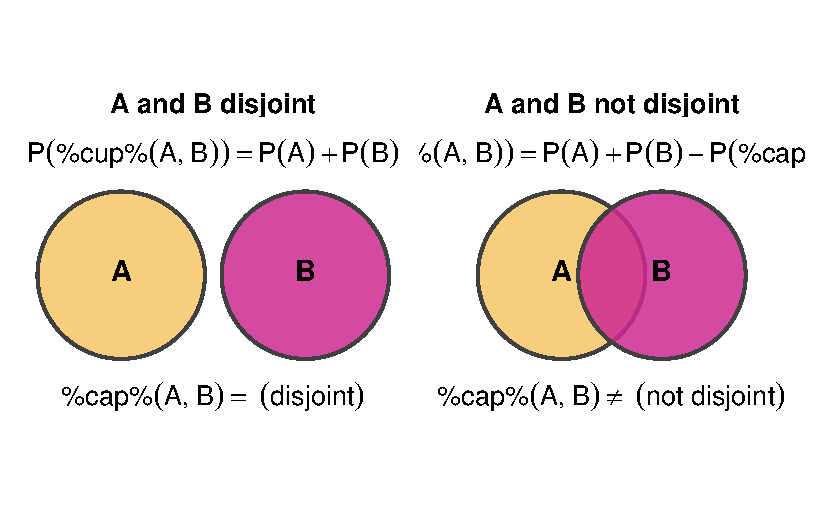
\includegraphics[keepaspectratio]{index_files/figure-pdf/unnamed-chunk-40-1.pdf}}

\subsection{The complement rule (Rule
4)}\label{the-complement-rule-rule-4}

The probability of an event \emph{not} occurring equals one minus the
probability that it \emph{does} occur:

{[} P(\text{not } A) = 1 - P(A) {]}

also implied, by rearranging the terms, is this:

{[} P(A) = 1 - P(\text{not } A) {]}

\subsection{Finite vs.~continuous probability
models}\label{finite-vs.-continuous-probability-models}

A \textbf{finite probability model} is one in which the sample space
consists of a \emph{discrete} and countable set of possible outcomes. In
such models, each outcome can be explicitly listed, and a probability is
assigned to each element of the sample space.\\
Typical examples include outcomes such as obtaining \emph{heads} or
\emph{tails} in a coin toss, selecting a political party from a
predefined list, observing the number of pips on a pair of dice, or
recording the number of days a student is absent during a semester.\\
Because the sample space is finite (or at least enumerable), the
probabilities of all possible outcomes must sum to 1:

{[} \sum\_i P(x\_i) = 1. {]}

In contrast, a \textbf{continuous probability model} has a
\emph{continuous} sample space---an uncountably infinite set of possible
values. Such models are used when outcomes are measured on a continuous
scale, as with \emph{height}, \emph{weight}, or \emph{time} to complete
a race. In practice, even variables that are recorded in rounded or
discrete units (e.g., test scores or height measured to the nearest
centimeter) are often treated as continuous when their possible values
are numerous and closely spaced.\\
In continuous models, probabilities are not assigned to individual
points but rather to \emph{intervals} of possible outcomes, using a
\textbf{probability density function (PDF)} represented by a smooth
density curve. The total area under the density curve equals 1:

{[} \int\_\{-\infty\}\^{}\{\infty\} f(x),dx = 1. {]}

Finite models are most appropriate for categorical or discrete numerical
outcomes, while continuous models describe probabilistic behavior over
measurable quantities that vary smoothly across a range of values.

\subsection{Probability models for discrete numerical
values}\label{probability-models-for-discrete-numerical-values}

Sometimes the basic outcomes are \textbf{discrete numerical counts}
rather than categories. In such cases we describe uncertainty with a
\textbf{probability mass function (pmf)} that assigns a probability to
each attainable count, with all probabilities non-negative and summing
to one. For example, a distribution for the \textbf{lifetime number of
children} places probability mass on the counts (0,1,2,3,4) and a
grouped tail category (\ge 5). The vertical spikes show the probability
attached to each count; the higher the spike, the more common that
outcome in the population. As always, the distribution must satisfy
(\sum\_\{x\} P(X=x)=1), so the heights of the spikes add up to one.

\begin{Shaded}
\begin{Highlighting}[]
\CommentTok{\#| echo: false}
\CommentTok{\#| message: false}
\CommentTok{\#| warning: false}
\CommentTok{\#| fig{-}width: 8}
\CommentTok{\#| fig{-}height: 5}
\CommentTok{\#| fig{-}cap: "Discrete pmf for daily coffee consumption: probabilities at counts 0–4 and a grouped tail (≥5)."}

\FunctionTok{library}\NormalTok{(ggplot2)}

\CommentTok{\# Example pmf for cups of coffee per day (sums to 1)}
\NormalTok{df }\OtherTok{\textless{}{-}} \FunctionTok{data.frame}\NormalTok{(}
  \AttributeTok{cups =} \FunctionTok{factor}\NormalTok{(}\FunctionTok{c}\NormalTok{(}\StringTok{"0"}\NormalTok{,}\StringTok{"1"}\NormalTok{,}\StringTok{"2"}\NormalTok{,}\StringTok{"3"}\NormalTok{,}\StringTok{"4"}\NormalTok{,}\StringTok{"≥5"}\NormalTok{),}
                \AttributeTok{levels =} \FunctionTok{c}\NormalTok{(}\StringTok{"0"}\NormalTok{,}\StringTok{"1"}\NormalTok{,}\StringTok{"2"}\NormalTok{,}\StringTok{"3"}\NormalTok{,}\StringTok{"4"}\NormalTok{,}\StringTok{"≥5"}\NormalTok{), }\AttributeTok{ordered =} \ConstantTok{TRUE}\NormalTok{),}
  \AttributeTok{p =} \FunctionTok{c}\NormalTok{(}\FloatTok{0.18}\NormalTok{, }\FloatTok{0.24}\NormalTok{, }\FloatTok{0.31}\NormalTok{, }\FloatTok{0.16}\NormalTok{, }\FloatTok{0.07}\NormalTok{, }\FloatTok{0.04}\NormalTok{)}
\NormalTok{)}

\CommentTok{\# Dark, flashy pink for spikes}
\NormalTok{pink }\OtherTok{\textless{}{-}} \StringTok{"\#E00070"}  \CommentTok{\# deep hot pink}

\FunctionTok{ggplot}\NormalTok{(df, }\FunctionTok{aes}\NormalTok{(}\AttributeTok{x =}\NormalTok{ cups, }\AttributeTok{y =}\NormalTok{ p)) }\SpecialCharTok{+}
  \CommentTok{\# stems}
  \FunctionTok{geom\_segment}\NormalTok{(}\FunctionTok{aes}\NormalTok{(}\AttributeTok{xend =}\NormalTok{ cups, }\AttributeTok{y =} \DecValTok{0}\NormalTok{, }\AttributeTok{yend =}\NormalTok{ p),}
               \AttributeTok{linewidth =} \FloatTok{2.2}\NormalTok{, }\AttributeTok{color =}\NormalTok{ pink) }\SpecialCharTok{+}
  \CommentTok{\# lollipop heads}
  \FunctionTok{geom\_point}\NormalTok{(}\AttributeTok{size =} \FloatTok{3.8}\NormalTok{, }\AttributeTok{color =}\NormalTok{ pink) }\SpecialCharTok{+}
  \CommentTok{\# axis \& limits}
  \FunctionTok{scale\_y\_continuous}\NormalTok{(}\AttributeTok{limits =} \FunctionTok{c}\NormalTok{(}\DecValTok{0}\NormalTok{, }\FunctionTok{max}\NormalTok{(df}\SpecialCharTok{$}\NormalTok{p) }\SpecialCharTok{*} \FloatTok{1.15}\NormalTok{), }
                     \AttributeTok{expand =} \FunctionTok{expansion}\NormalTok{(}\AttributeTok{mult =} \FunctionTok{c}\NormalTok{(}\DecValTok{0}\NormalTok{, .}\DecValTok{02}\NormalTok{))) }\SpecialCharTok{+}
  \FunctionTok{labs}\NormalTok{(}\AttributeTok{x =} \StringTok{"cups of coffee per day"}\NormalTok{, }
       \AttributeTok{y =} \StringTok{"probability"}\NormalTok{) }\SpecialCharTok{+}
  \FunctionTok{theme\_classic}\NormalTok{(}\AttributeTok{base\_size =} \DecValTok{14}\NormalTok{) }\SpecialCharTok{+}
  \FunctionTok{theme}\NormalTok{(}
    \AttributeTok{axis.title =} \FunctionTok{element\_text}\NormalTok{(}\AttributeTok{face =} \StringTok{"bold"}\NormalTok{),}
    \AttributeTok{axis.text.x =} \FunctionTok{element\_text}\NormalTok{(}\AttributeTok{margin =} \FunctionTok{margin}\NormalTok{(}\AttributeTok{t =} \DecValTok{6}\NormalTok{)),}
    \AttributeTok{axis.text.y =} \FunctionTok{element\_text}\NormalTok{(}\AttributeTok{margin =} \FunctionTok{margin}\NormalTok{(}\AttributeTok{r =} \DecValTok{6}\NormalTok{)),}
    \AttributeTok{panel.grid.major.y =} \FunctionTok{element\_line}\NormalTok{(}\AttributeTok{color =} \StringTok{"grey85"}\NormalTok{, }
                                      \AttributeTok{linewidth =} \FloatTok{0.4}\NormalTok{, }
                                      \AttributeTok{linetype =} \StringTok{"dotted"}\NormalTok{),}
    \AttributeTok{panel.grid.minor =} \FunctionTok{element\_blank}\NormalTok{()}
\NormalTok{  )}
\end{Highlighting}
\end{Shaded}

\pandocbounded{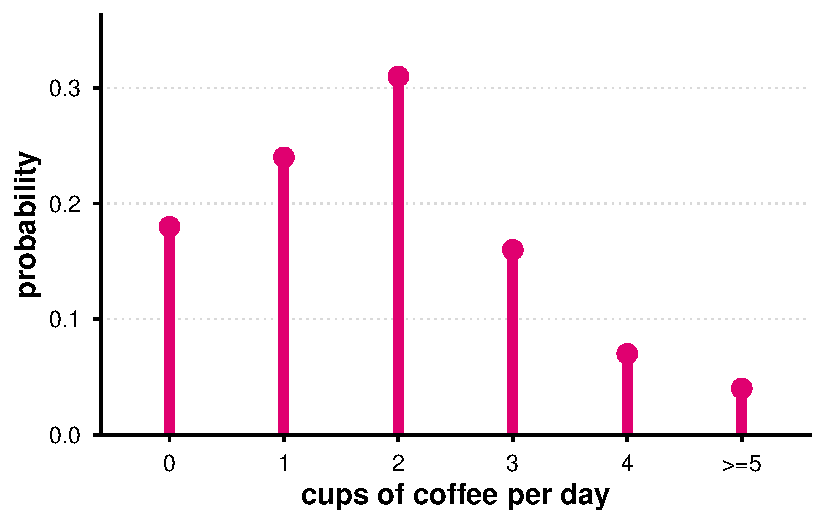
\includegraphics[keepaspectratio]{index_files/figure-pdf/unnamed-chunk-41-1.pdf}}

\subsection{Probability models for continuous numerical
variables}\label{probability-models-for-continuous-numerical-variables}

A \textbf{continuous} sample space contains an uncountable infinity of
values between any two points. For example, the interval ({[}0,1{]})
contains infinitely many real numbers (e.g., (0.1, 0.15, 0.155, 0.1555,
\ldots)). In a continuous probability model the sample space can be
written as {[} S = \{,x : 0 \le x \le 1,\}. {]} Probabilities are
assigned \textbf{to intervals}, not to individual points, via a
\textbf{probability density function} (f(x)). The probability that (X)
falls in an interval is the \textbf{area under the density curve} over
that interval. For the uniform model on ({[}0,1{]}), (f(x)=1) for
(0\le x\le 1), so {[} \Pr(0.3 \le X \le 0.7) ;=;
\int\_\{0.3\}\^{}\{0.7\} 1,dx ;=; 0.4, {]} which equals the width of the
interval.

\begin{Shaded}
\begin{Highlighting}[]
\CommentTok{\#| echo: false}
\CommentTok{\#| message: false}
\CommentTok{\#| warning: false}
\CommentTok{\#| fig{-}width: 8}
\CommentTok{\#| fig{-}height: 4.8}
\CommentTok{\#| fig{-}cap: "Uniform(0,1) density: probabilities are areas. Here the shaded interval [0.3, 0.7] has area 0.4."}

\FunctionTok{library}\NormalTok{(ggplot2)}

\CommentTok{\# A flashy dark pink}
\NormalTok{pink }\OtherTok{\textless{}{-}} \StringTok{"\#E00070"}

\CommentTok{\# Data frames for the base line and the shaded interval}
\NormalTok{df\_base }\OtherTok{\textless{}{-}} \FunctionTok{data.frame}\NormalTok{(}\AttributeTok{x =} \FunctionTok{c}\NormalTok{(}\DecValTok{0}\NormalTok{, }\DecValTok{1}\NormalTok{), }\AttributeTok{y =} \DecValTok{1}\NormalTok{)   }\CommentTok{\# density level}
\NormalTok{df\_fill }\OtherTok{\textless{}{-}} \FunctionTok{data.frame}\NormalTok{(}\AttributeTok{xmin =} \FloatTok{0.3}\NormalTok{, }\AttributeTok{xmax =} \FloatTok{0.7}\NormalTok{, }\AttributeTok{ymin =} \DecValTok{0}\NormalTok{, }\AttributeTok{ymax =} \DecValTok{1}\NormalTok{)}

\FunctionTok{ggplot}\NormalTok{() }\SpecialCharTok{+}
  \CommentTok{\# Shaded probability for [0.3, 0.7]}
  \FunctionTok{geom\_rect}\NormalTok{(}\AttributeTok{data =}\NormalTok{ df\_fill,}
            \FunctionTok{aes}\NormalTok{(}\AttributeTok{xmin =}\NormalTok{ xmin, }\AttributeTok{xmax =}\NormalTok{ xmax, }\AttributeTok{ymin =}\NormalTok{ ymin, }\AttributeTok{ymax =}\NormalTok{ ymax),}
            \AttributeTok{fill =}\NormalTok{ scales}\SpecialCharTok{::}\FunctionTok{alpha}\NormalTok{(pink, }\FloatTok{0.35}\NormalTok{), }\AttributeTok{color =} \ConstantTok{NA}\NormalTok{) }\SpecialCharTok{+}
  \CommentTok{\# Density "curve" for Uniform(0,1) (height = 1)}
  \FunctionTok{geom\_segment}\NormalTok{(}\FunctionTok{aes}\NormalTok{(}\AttributeTok{x =} \DecValTok{0}\NormalTok{, }\AttributeTok{xend =} \DecValTok{1}\NormalTok{, }\AttributeTok{y =} \DecValTok{1}\NormalTok{, }\AttributeTok{yend =} \DecValTok{1}\NormalTok{), }\AttributeTok{linewidth =} \FloatTok{1.1}\NormalTok{) }\SpecialCharTok{+}
  \CommentTok{\# Vertical boundaries 0, 1 and interval ticks 0.3, 0.7}
  \FunctionTok{geom\_segment}\NormalTok{(}\FunctionTok{aes}\NormalTok{(}\AttributeTok{x =} \DecValTok{0}\NormalTok{,   }\AttributeTok{xend =} \DecValTok{0}\NormalTok{,   }\AttributeTok{y =} \DecValTok{0}\NormalTok{, }\AttributeTok{yend =} \DecValTok{1}\NormalTok{), }\AttributeTok{linewidth =} \FloatTok{0.8}\NormalTok{) }\SpecialCharTok{+}
  \FunctionTok{geom\_segment}\NormalTok{(}\FunctionTok{aes}\NormalTok{(}\AttributeTok{x =} \DecValTok{1}\NormalTok{,   }\AttributeTok{xend =} \DecValTok{1}\NormalTok{,   }\AttributeTok{y =} \DecValTok{0}\NormalTok{, }\AttributeTok{yend =} \DecValTok{1}\NormalTok{), }\AttributeTok{linewidth =} \FloatTok{0.8}\NormalTok{) }\SpecialCharTok{+}
  \FunctionTok{geom\_segment}\NormalTok{(}\FunctionTok{aes}\NormalTok{(}\AttributeTok{x =} \FloatTok{0.3}\NormalTok{, }\AttributeTok{xend =} \FloatTok{0.3}\NormalTok{, }\AttributeTok{y =} \DecValTok{0}\NormalTok{, }\AttributeTok{yend =} \DecValTok{1}\NormalTok{),}
               \AttributeTok{linewidth =} \FloatTok{0.9}\NormalTok{, }\AttributeTok{color =}\NormalTok{ pink) }\SpecialCharTok{+}
  \FunctionTok{geom\_segment}\NormalTok{(}\FunctionTok{aes}\NormalTok{(}\AttributeTok{x =} \FloatTok{0.7}\NormalTok{, }\AttributeTok{xend =} \FloatTok{0.7}\NormalTok{, }\AttributeTok{y =} \DecValTok{0}\NormalTok{, }\AttributeTok{yend =} \DecValTok{1}\NormalTok{),}
               \AttributeTok{linewidth =} \FloatTok{0.9}\NormalTok{, }\AttributeTok{color =}\NormalTok{ pink) }\SpecialCharTok{+}
  \CommentTok{\# Labels (no parse; use Unicode ≤ to avoid plotmath parsing issues)}
  \FunctionTok{annotate}\NormalTok{(}\StringTok{"text"}\NormalTok{, }\AttributeTok{x =} \FloatTok{0.5}\NormalTok{, }\AttributeTok{y =} \FloatTok{1.06}\NormalTok{,}
           \AttributeTok{label =} \StringTok{"Height = 1"}\NormalTok{, }\AttributeTok{fontface =} \StringTok{"bold"}\NormalTok{) }\SpecialCharTok{+}
  \FunctionTok{annotate}\NormalTok{(}\StringTok{"text"}\NormalTok{, }\AttributeTok{x =} \FloatTok{0.72}\NormalTok{, }\AttributeTok{y =} \FloatTok{0.85}\NormalTok{,}
           \AttributeTok{label =} \StringTok{"Probability = Area = 0.4"}\NormalTok{, }\AttributeTok{fontface =} \StringTok{"bold"}\NormalTok{) }\SpecialCharTok{+}
  \FunctionTok{annotate}\NormalTok{(}\StringTok{"text"}\NormalTok{, }\AttributeTok{x =} \FloatTok{0.5}\NormalTok{, }\AttributeTok{y =} \FloatTok{0.12}\NormalTok{,}
           \AttributeTok{label =} \StringTok{"P(0.3 \textbackslash{}u2264 X \textbackslash{}u2264 0.7) = 0.4"}\NormalTok{) }\SpecialCharTok{+}
  \CommentTok{\# Axes}
  \FunctionTok{scale\_x\_continuous}\NormalTok{(}\AttributeTok{breaks =} \FunctionTok{c}\NormalTok{(}\DecValTok{0}\NormalTok{, }\FloatTok{0.3}\NormalTok{, }\FloatTok{0.7}\NormalTok{, }\DecValTok{1}\NormalTok{),}
                     \AttributeTok{labels =} \FunctionTok{c}\NormalTok{(}\StringTok{"0"}\NormalTok{, }\StringTok{"0.3"}\NormalTok{, }\StringTok{"0.7"}\NormalTok{, }\StringTok{"1"}\NormalTok{),}
                     \AttributeTok{limits =} \FunctionTok{c}\NormalTok{(}\SpecialCharTok{{-}}\FloatTok{0.02}\NormalTok{, }\FloatTok{1.02}\NormalTok{),}
                     \AttributeTok{expand =} \FunctionTok{c}\NormalTok{(}\DecValTok{0}\NormalTok{, }\DecValTok{0}\NormalTok{)) }\SpecialCharTok{+}
  \FunctionTok{scale\_y\_continuous}\NormalTok{(}\AttributeTok{breaks =} \FunctionTok{c}\NormalTok{(}\DecValTok{0}\NormalTok{, }\FloatTok{0.5}\NormalTok{, }\DecValTok{1}\NormalTok{),}
                     \AttributeTok{limits =} \FunctionTok{c}\NormalTok{(}\DecValTok{0}\NormalTok{, }\FloatTok{1.1}\NormalTok{),}
                     \AttributeTok{expand =} \FunctionTok{c}\NormalTok{(}\DecValTok{0}\NormalTok{, }\FloatTok{0.02}\NormalTok{)) }\SpecialCharTok{+}
  \FunctionTok{labs}\NormalTok{(}\AttributeTok{x =} \ConstantTok{NULL}\NormalTok{, }\AttributeTok{y =} \ConstantTok{NULL}\NormalTok{) }\SpecialCharTok{+}
  \FunctionTok{theme\_classic}\NormalTok{(}\AttributeTok{base\_size =} \DecValTok{14}\NormalTok{) }\SpecialCharTok{+}
  \FunctionTok{theme}\NormalTok{(}
    \AttributeTok{axis.line =} \FunctionTok{element\_blank}\NormalTok{(),}
    \AttributeTok{axis.ticks =} \FunctionTok{element\_blank}\NormalTok{(),}
    \AttributeTok{panel.grid.major.y =} \FunctionTok{element\_line}\NormalTok{(}\AttributeTok{color =} \StringTok{"grey88"}\NormalTok{, }\AttributeTok{linewidth =} \FloatTok{0.4}\NormalTok{, }\AttributeTok{linetype =} \StringTok{"dotted"}\NormalTok{),}
    \AttributeTok{panel.grid.major.x =} \FunctionTok{element\_line}\NormalTok{(}\AttributeTok{color =} \StringTok{"grey92"}\NormalTok{, }\AttributeTok{linewidth =} \FloatTok{0.4}\NormalTok{, }\AttributeTok{linetype =} \StringTok{"dotted"}\NormalTok{),}
    \AttributeTok{plot.margin =} \FunctionTok{margin}\NormalTok{(}\DecValTok{10}\NormalTok{, }\DecValTok{10}\NormalTok{, }\DecValTok{6}\NormalTok{, }\DecValTok{10}\NormalTok{)}
\NormalTok{  )}
\end{Highlighting}
\end{Shaded}

\pandocbounded{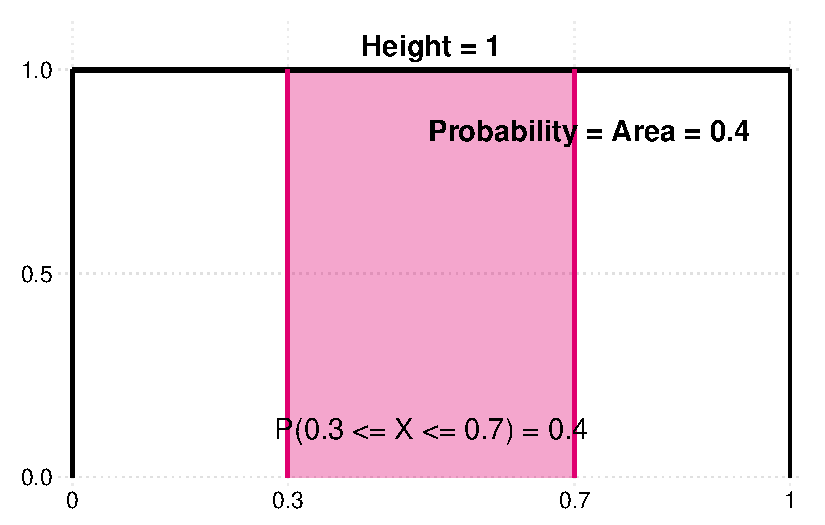
\includegraphics[keepaspectratio]{index_files/figure-pdf/unnamed-chunk-42-1.pdf}}

\begin{Shaded}
\begin{Highlighting}[]
\FunctionTok{annotate}\NormalTok{(}\StringTok{"text"}\NormalTok{, }\AttributeTok{x=}\NormalTok{.}\DecValTok{5}\NormalTok{, }\AttributeTok{y=}\NormalTok{.}\DecValTok{12}\NormalTok{, }\AttributeTok{label=}\StringTok{"P(0.3 \textless{}= X) == 0.4 + P(X \textgreater{} 0.7)"}\NormalTok{, }\AttributeTok{parse=}\ConstantTok{TRUE}\NormalTok{)}
\end{Highlighting}
\end{Shaded}

\begin{verbatim}
mapping: x = ~x, y = ~y 
geom_text: na.rm = FALSE, parse = TRUE
stat_identity: na.rm = FALSE
position_identity 
\end{verbatim}

\begin{Shaded}
\begin{Highlighting}[]
\CommentTok{\# or}
\FunctionTok{annotate}\NormalTok{(}\StringTok{"text"}\NormalTok{, }\AttributeTok{x=}\NormalTok{.}\DecValTok{5}\NormalTok{, }\AttributeTok{y=}\NormalTok{.}\DecValTok{12}\NormalTok{, }\AttributeTok{label=}\StringTok{"P(bold(}\SpecialCharTok{\textbackslash{}"}\StringTok{0.3 \textbackslash{}u2264 X \textbackslash{}u2264 0.7}\SpecialCharTok{\textbackslash{}"}\StringTok{)) == 0.4"}\NormalTok{)}
\end{Highlighting}
\end{Shaded}

\begin{verbatim}
mapping: x = ~x, y = ~y 
geom_text: na.rm = FALSE
stat_identity: na.rm = FALSE
position_identity 
\end{verbatim}

\subsection{Probabilities from other density
curves}\label{probabilities-from-other-density-curves}

So far, we have used uniform densities to describe probabilities over
equal-width intervals. Many real-world quantities, however, follow
\textbf{non-uniform} distributions.\\
For instance, the distribution of women's heights in the U.S. is
approximately normal: {[} X \sim N(\mu, \sigma) = N(64.5, 2.5) {]} where
the mean height is (64.5) inches and the standard deviation is (2.5)
inches.

Suppose we ask: \emph{What proportion of women have heights between
59.5″ and 69.5″?}\\
These bounds are roughly ±2 standard deviations from the mean, and for a
normal distribution the area between them is about \textbf{0.95}.

Thus, about 95 \% of women fall in that interval, and the
\textbf{probability} of randomly selecting one such woman is also
approximately 0.95.\\
In this sense, the \emph{proportion under the curve} directly
corresponds to the \emph{probability of selection} when sampling from
the population.

\subsection{The Empirical Rule: 68--95--99.7 for Normal
Distributions}\label{the-empirical-rule-689599.7-for-normal-distributions}

In a normal distribution, most of the data cluster around the mean, and
probabilities can be described using the \textbf{empirical rule}:

\begin{itemize}
\tightlist
\item
  Approximately \textbf{68\%} of values fall within one standard
  deviation (σ) of the mean (μ).\\
\item
  Approximately \textbf{95\%} fall within two standard deviations.\\
\item
  Approximately \textbf{99.7\%} fall within three standard deviations.
\end{itemize}

These proportions represent the cumulative areas under the density curve
between μ ± 1σ, μ ± 2σ, and μ ± 3σ.

\begin{Shaded}
\begin{Highlighting}[]
\CommentTok{\#| echo: false}
\CommentTok{\#| message: false}
\CommentTok{\#| warning: false}
\CommentTok{\#| fig{-}width: 8}
\CommentTok{\#| fig{-}height: 5.5}
\CommentTok{\#| fig{-}cap: "The empirical 68–95–99.7 rule for the normal distribution."}

\FunctionTok{library}\NormalTok{(ggplot2)}

\CommentTok{\# Parameters}
\NormalTok{mu }\OtherTok{\textless{}{-}} \FloatTok{64.5}
\NormalTok{sigma }\OtherTok{\textless{}{-}} \FloatTok{2.5}
\NormalTok{x }\OtherTok{\textless{}{-}} \FunctionTok{seq}\NormalTok{(mu }\SpecialCharTok{{-}} \DecValTok{4}\SpecialCharTok{*}\NormalTok{sigma, mu }\SpecialCharTok{+} \DecValTok{4}\SpecialCharTok{*}\NormalTok{sigma, }\AttributeTok{length.out =} \DecValTok{800}\NormalTok{)}
\NormalTok{y }\OtherTok{\textless{}{-}} \FunctionTok{dnorm}\NormalTok{(x, mu, sigma)}
\NormalTok{df }\OtherTok{\textless{}{-}} \FunctionTok{data.frame}\NormalTok{(x, y)}

\CommentTok{\# Define shading areas}
\NormalTok{shade\_1 }\OtherTok{\textless{}{-}} \FunctionTok{subset}\NormalTok{(df, x }\SpecialCharTok{\textgreater{}=}\NormalTok{ mu }\SpecialCharTok{{-}}\NormalTok{ sigma }\SpecialCharTok{\&}\NormalTok{ x }\SpecialCharTok{\textless{}=}\NormalTok{ mu }\SpecialCharTok{+}\NormalTok{ sigma)}
\NormalTok{shade\_2 }\OtherTok{\textless{}{-}} \FunctionTok{subset}\NormalTok{(df, x }\SpecialCharTok{\textgreater{}=}\NormalTok{ mu }\SpecialCharTok{{-}} \DecValTok{2}\SpecialCharTok{*}\NormalTok{sigma }\SpecialCharTok{\&}\NormalTok{ x }\SpecialCharTok{\textless{}=}\NormalTok{ mu }\SpecialCharTok{+} \DecValTok{2}\SpecialCharTok{*}\NormalTok{sigma)}
\NormalTok{shade\_3 }\OtherTok{\textless{}{-}} \FunctionTok{subset}\NormalTok{(df, x }\SpecialCharTok{\textgreater{}=}\NormalTok{ mu }\SpecialCharTok{{-}} \DecValTok{3}\SpecialCharTok{*}\NormalTok{sigma }\SpecialCharTok{\&}\NormalTok{ x }\SpecialCharTok{\textless{}=}\NormalTok{ mu }\SpecialCharTok{+} \DecValTok{3}\SpecialCharTok{*}\NormalTok{sigma)}

\CommentTok{\# Colors — Matinain Pink palette}
\NormalTok{deep\_pink }\OtherTok{\textless{}{-}} \StringTok{"\#E00070"}
\NormalTok{mid\_pink  }\OtherTok{\textless{}{-}} \StringTok{"\#F3C1D7"}
\NormalTok{light\_pink }\OtherTok{\textless{}{-}} \StringTok{"\#F9E0EC"}
\NormalTok{outline }\OtherTok{\textless{}{-}}\NormalTok{ deep\_pink}

\CommentTok{\# Plot}
\FunctionTok{ggplot}\NormalTok{(df, }\FunctionTok{aes}\NormalTok{(x, y)) }\SpecialCharTok{+}
  \CommentTok{\# Shaded regions for 1σ, 2σ, 3σ}
  \FunctionTok{geom\_area}\NormalTok{(}\AttributeTok{data =}\NormalTok{ shade\_3, }\FunctionTok{aes}\NormalTok{(}\AttributeTok{y =}\NormalTok{ y), }\AttributeTok{fill =}\NormalTok{ light\_pink) }\SpecialCharTok{+}
  \FunctionTok{geom\_area}\NormalTok{(}\AttributeTok{data =}\NormalTok{ shade\_2, }\FunctionTok{aes}\NormalTok{(}\AttributeTok{y =}\NormalTok{ y), }\AttributeTok{fill =}\NormalTok{ mid\_pink) }\SpecialCharTok{+}
  \FunctionTok{geom\_area}\NormalTok{(}\AttributeTok{data =}\NormalTok{ shade\_1, }\FunctionTok{aes}\NormalTok{(}\AttributeTok{y =}\NormalTok{ y), }\AttributeTok{fill =}\NormalTok{ deep\_pink, }\AttributeTok{alpha =} \FloatTok{0.55}\NormalTok{) }\SpecialCharTok{+}

  \CommentTok{\# Main curve}
  \FunctionTok{geom\_line}\NormalTok{(}\AttributeTok{color =}\NormalTok{ outline, }\AttributeTok{linewidth =} \FloatTok{1.2}\NormalTok{) }\SpecialCharTok{+}

  \CommentTok{\# Vertical lines at μ ± 1σ, 2σ, 3σ}
  \FunctionTok{geom\_vline}\NormalTok{(}\AttributeTok{xintercept =}\NormalTok{ mu }\SpecialCharTok{+} \FunctionTok{c}\NormalTok{(}\SpecialCharTok{{-}}\DecValTok{1}\NormalTok{, }\DecValTok{0}\NormalTok{, }\DecValTok{1}\NormalTok{)}\SpecialCharTok{*}\NormalTok{sigma,}
             \AttributeTok{color =}\NormalTok{ outline, }\AttributeTok{linetype =} \FunctionTok{c}\NormalTok{(}\StringTok{"dashed"}\NormalTok{, }\StringTok{"solid"}\NormalTok{, }\StringTok{"dashed"}\NormalTok{),}
             \AttributeTok{linewidth =} \FloatTok{0.7}\NormalTok{) }\SpecialCharTok{+}
  \FunctionTok{geom\_vline}\NormalTok{(}\AttributeTok{xintercept =}\NormalTok{ mu }\SpecialCharTok{+} \FunctionTok{c}\NormalTok{(}\SpecialCharTok{{-}}\DecValTok{2}\NormalTok{, }\DecValTok{2}\NormalTok{)}\SpecialCharTok{*}\NormalTok{sigma, }\AttributeTok{color =}\NormalTok{ outline,}
             \AttributeTok{linetype =} \StringTok{"dotted"}\NormalTok{, }\AttributeTok{linewidth =} \FloatTok{0.6}\NormalTok{) }\SpecialCharTok{+}
  \FunctionTok{geom\_vline}\NormalTok{(}\AttributeTok{xintercept =}\NormalTok{ mu }\SpecialCharTok{+} \FunctionTok{c}\NormalTok{(}\SpecialCharTok{{-}}\DecValTok{3}\NormalTok{, }\DecValTok{3}\NormalTok{)}\SpecialCharTok{*}\NormalTok{sigma, }\AttributeTok{color =}\NormalTok{ outline,}
             \AttributeTok{linetype =} \StringTok{"dotted"}\NormalTok{, }\AttributeTok{linewidth =} \FloatTok{0.5}\NormalTok{) }\SpecialCharTok{+}

  \CommentTok{\# Text annotations for 68–95–99.7 in black}
  \FunctionTok{annotate}\NormalTok{(}\StringTok{"text"}\NormalTok{, }\AttributeTok{x =}\NormalTok{ mu, }\AttributeTok{y =} \FloatTok{0.13}\NormalTok{, }\AttributeTok{label =} \StringTok{"68\%"}\NormalTok{, }\AttributeTok{color =} \StringTok{"black"}\NormalTok{,}
           \AttributeTok{fontface =} \StringTok{"bold"}\NormalTok{, }\AttributeTok{size =} \DecValTok{5}\NormalTok{) }\SpecialCharTok{+}
  \FunctionTok{annotate}\NormalTok{(}\StringTok{"text"}\NormalTok{, }\AttributeTok{x =}\NormalTok{ mu, }\AttributeTok{y =} \FloatTok{0.085}\NormalTok{, }\AttributeTok{label =} \StringTok{"95\%"}\NormalTok{, }\AttributeTok{color =} \StringTok{"black"}\NormalTok{,}
           \AttributeTok{fontface =} \StringTok{"bold"}\NormalTok{, }\AttributeTok{size =} \DecValTok{5}\NormalTok{) }\SpecialCharTok{+}
  \FunctionTok{annotate}\NormalTok{(}\StringTok{"text"}\NormalTok{, }\AttributeTok{x =}\NormalTok{ mu, }\AttributeTok{y =} \FloatTok{0.045}\NormalTok{, }\AttributeTok{label =} \StringTok{"99.7\%"}\NormalTok{, }\AttributeTok{color =} \StringTok{"black"}\NormalTok{,}
           \AttributeTok{fontface =} \StringTok{"bold"}\NormalTok{, }\AttributeTok{size =} \DecValTok{5}\NormalTok{) }\SpecialCharTok{+}

  \CommentTok{\# Arrows showing intervals}
  \FunctionTok{annotate}\NormalTok{(}\StringTok{"segment"}\NormalTok{, }\AttributeTok{x =}\NormalTok{ mu }\SpecialCharTok{{-}}\NormalTok{ sigma, }\AttributeTok{xend =}\NormalTok{ mu }\SpecialCharTok{+}\NormalTok{ sigma, }\AttributeTok{y =} \FloatTok{0.12}\NormalTok{, }\AttributeTok{yend =} \FloatTok{0.12}\NormalTok{,}
           \AttributeTok{arrow =} \FunctionTok{arrow}\NormalTok{(}\AttributeTok{length =} \FunctionTok{unit}\NormalTok{(}\FloatTok{0.2}\NormalTok{, }\StringTok{"cm"}\NormalTok{)), }\AttributeTok{color =}\NormalTok{ outline) }\SpecialCharTok{+}
  \FunctionTok{annotate}\NormalTok{(}\StringTok{"segment"}\NormalTok{, }\AttributeTok{x =}\NormalTok{ mu }\SpecialCharTok{{-}} \DecValTok{2}\SpecialCharTok{*}\NormalTok{sigma, }\AttributeTok{xend =}\NormalTok{ mu }\SpecialCharTok{+} \DecValTok{2}\SpecialCharTok{*}\NormalTok{sigma, }\AttributeTok{y =} \FloatTok{0.075}\NormalTok{, }\AttributeTok{yend =} \FloatTok{0.075}\NormalTok{,}
           \AttributeTok{arrow =} \FunctionTok{arrow}\NormalTok{(}\AttributeTok{length =} \FunctionTok{unit}\NormalTok{(}\FloatTok{0.2}\NormalTok{, }\StringTok{"cm"}\NormalTok{)), }\AttributeTok{color =}\NormalTok{ outline) }\SpecialCharTok{+}
  \FunctionTok{annotate}\NormalTok{(}\StringTok{"segment"}\NormalTok{, }\AttributeTok{x =}\NormalTok{ mu }\SpecialCharTok{{-}} \DecValTok{3}\SpecialCharTok{*}\NormalTok{sigma, }\AttributeTok{xend =}\NormalTok{ mu }\SpecialCharTok{+} \DecValTok{3}\SpecialCharTok{*}\NormalTok{sigma, }\AttributeTok{y =} \FloatTok{0.035}\NormalTok{, }\AttributeTok{yend =} \FloatTok{0.035}\NormalTok{,}
           \AttributeTok{arrow =} \FunctionTok{arrow}\NormalTok{(}\AttributeTok{length =} \FunctionTok{unit}\NormalTok{(}\FloatTok{0.2}\NormalTok{, }\StringTok{"cm"}\NormalTok{)), }\AttributeTok{color =}\NormalTok{ outline) }\SpecialCharTok{+}

  \CommentTok{\# Labels and theme}
  \FunctionTok{labs}\NormalTok{(}\AttributeTok{x =} \StringTok{"Height (in inches)"}\NormalTok{, }\AttributeTok{y =} \StringTok{"Density"}\NormalTok{) }\SpecialCharTok{+}
  \FunctionTok{theme\_minimal}\NormalTok{(}\AttributeTok{base\_size =} \DecValTok{14}\NormalTok{) }\SpecialCharTok{+}
  \FunctionTok{theme}\NormalTok{(}
    \AttributeTok{plot.background =} \FunctionTok{element\_rect}\NormalTok{(}\AttributeTok{fill =} \StringTok{"white"}\NormalTok{, }\AttributeTok{color =} \ConstantTok{NA}\NormalTok{),}
    \AttributeTok{panel.grid =} \FunctionTok{element\_blank}\NormalTok{(),}
    \AttributeTok{axis.line =} \FunctionTok{element\_line}\NormalTok{(}\AttributeTok{color =} \StringTok{"black"}\NormalTok{),}
    \AttributeTok{axis.title =} \FunctionTok{element\_text}\NormalTok{(}\AttributeTok{face =} \StringTok{"bold"}\NormalTok{),}
    \AttributeTok{axis.text =} \FunctionTok{element\_text}\NormalTok{(}\AttributeTok{color =} \StringTok{"black"}\NormalTok{)}
\NormalTok{  )}
\end{Highlighting}
\end{Shaded}

\pandocbounded{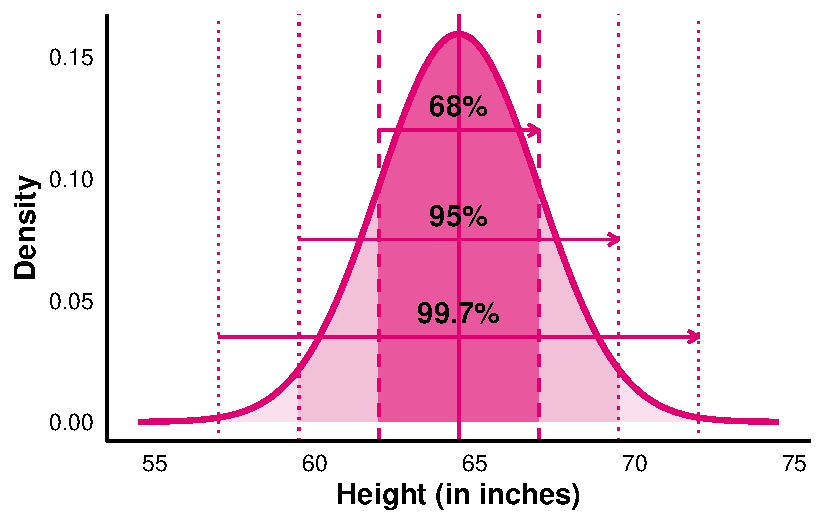
\includegraphics[keepaspectratio]{index_files/figure-pdf/unnamed-chunk-43-1.pdf}}

\subsection{Probabilities from a normal density: the 68--95--99.7
rule}\label{probabilities-from-a-normal-density-the-689599.7-rule}

If (X \sim N(\mu,\sigma)), the \emph{empirical rule} states that about
\textbf{68\%} of the distribution lies within one standard deviation of
the mean ({[}\mu-\sigma,~\mu+\sigma{]}), about \textbf{95\%} lies within
two standard deviations ({[}\mu-2\sigma,~\mu+2\sigma{]}), and about
\textbf{99.7\%} lies within three standard deviations
({[}\mu-3\sigma,~\mu+3\sigma{]}). The figure below shows this for
women's heights, modeled as (N(64.5,~2.5)) inches: the curve is the
density, the green \textbf{arrows} span the one-, two-, and three-sigma
intervals, and the vertical guides mark the boundaries at
(\mu \pm \sigma), (\mu \pm 2\sigma), and (\mu \pm 3\sigma). Areas under
the curve over those spans correspond to the listed percentages.

\subsubsection{\texorpdfstring{Empirical rule for
(N(\mu,\sigma))}{Empirical rule for (N(,))}}\label{empirical-rule-for-n}

If (X \sim N(\mu,\sigma)), about \textbf{68\%} of values fall in
({[}\mu-\sigma,~\mu+\sigma{]}), about \textbf{95\%} in
({[}\mu-2\sigma,~\mu+2\sigma{]}), and about \textbf{99.7\%} in
({[}\mu-3\sigma,~\mu+3\sigma{]}).\\
For women's heights (N(64.5,~2.5)) (inches), the density curve shows
green \textbf{arrows} spanning the one-, two-, and three-sigma
intervals; vertical guides mark (\mu \pm \sigma), (\mu \pm 2\sigma), and
(\mu \pm 3\sigma). The corresponding shaded areas equal the stated
percentages.

\begin{Shaded}
\begin{Highlighting}[]
\CommentTok{\#| echo: false}
\CommentTok{\#| message: false}
\CommentTok{\#| warning: false}

\CommentTok{\# We\textquotesingle{}ll use htmltools to construct HTML safely (no cat)}
\FunctionTok{library}\NormalTok{(htmltools)}

\FunctionTok{set.seed}\NormalTok{(}\DecValTok{42}\NormalTok{)}

\CommentTok{\# {-}{-}{-}{-}{-}{-}{-}{-}{-}{-} Demo population (replace with your real data if you like) {-}{-}{-}{-}{-}{-}{-}{-}{-}{-}}
\NormalTok{states }\OtherTok{\textless{}{-}} \FunctionTok{c}\NormalTok{(state.name, }\StringTok{"District of Columbia"}\NormalTok{)}
\NormalTok{N }\OtherTok{\textless{}{-}} \FunctionTok{length}\NormalTok{(states)}
\NormalTok{rate }\OtherTok{\textless{}{-}} \FunctionTok{round}\NormalTok{(}\FunctionTok{pmax}\NormalTok{(}\FunctionTok{rnorm}\NormalTok{(N, }\AttributeTok{mean =} \FloatTok{5.3}\NormalTok{, }\AttributeTok{sd =} \FloatTok{2.0}\NormalTok{), }\FloatTok{0.1}\NormalTok{), }\DecValTok{1}\NormalTok{)}
\NormalTok{pop  }\OtherTok{\textless{}{-}} \FunctionTok{data.frame}\NormalTok{(}\AttributeTok{state =}\NormalTok{ states, }\AttributeTok{murder =}\NormalTok{ rate, }\AttributeTok{stringsAsFactors =} \ConstantTok{FALSE}\NormalTok{)}
\NormalTok{mu   }\OtherTok{\textless{}{-}} \FunctionTok{round}\NormalTok{(}\FunctionTok{mean}\NormalTok{(pop}\SpecialCharTok{$}\NormalTok{murder), }\DecValTok{2}\NormalTok{)}

\CommentTok{\# Two SRS samples of size 5}
\NormalTok{samp }\OtherTok{\textless{}{-}} \ControlFlowTok{function}\NormalTok{() pop[}\FunctionTok{sample.int}\NormalTok{(N, }\DecValTok{5}\NormalTok{, }\AttributeTok{replace =} \ConstantTok{FALSE}\NormalTok{), }\FunctionTok{c}\NormalTok{(}\StringTok{"state"}\NormalTok{,}\StringTok{"murder"}\NormalTok{)]}
\NormalTok{s1 }\OtherTok{\textless{}{-}} \FunctionTok{samp}\NormalTok{(); s2 }\OtherTok{\textless{}{-}} \FunctionTok{samp}\NormalTok{()}
\NormalTok{s1\_mean }\OtherTok{\textless{}{-}} \FunctionTok{sprintf}\NormalTok{(}\StringTok{"\%.2f"}\NormalTok{, }\FunctionTok{mean}\NormalTok{(s1}\SpecialCharTok{$}\NormalTok{murder))}
\NormalTok{s2\_mean }\OtherTok{\textless{}{-}} \FunctionTok{sprintf}\NormalTok{(}\StringTok{"\%.2f"}\NormalTok{, }\FunctionTok{mean}\NormalTok{(s2}\SpecialCharTok{$}\NormalTok{murder))}

\CommentTok{\# Split population into two columns (1..26) and (27..51)}
\NormalTok{left  }\OtherTok{\textless{}{-}} \FunctionTok{transform}\NormalTok{(pop[}\DecValTok{1}\SpecialCharTok{:}\DecValTok{26}\NormalTok{, ], }\AttributeTok{idx =} \FunctionTok{sprintf}\NormalTok{(}\StringTok{"\%2d."}\NormalTok{, }\DecValTok{1}\SpecialCharTok{:}\DecValTok{26}\NormalTok{))}
\NormalTok{right }\OtherTok{\textless{}{-}} \FunctionTok{transform}\NormalTok{(pop[}\DecValTok{27}\SpecialCharTok{:}\DecValTok{51}\NormalTok{,], }\AttributeTok{idx =} \FunctionTok{sprintf}\NormalTok{(}\StringTok{"\%2d."}\NormalTok{, }\DecValTok{27}\SpecialCharTok{:}\DecValTok{51}\NormalTok{))}

\CommentTok{\# {-}{-}{-}{-}{-}{-}{-}{-}{-}{-} CSS (injected via htmltools; no cat) {-}{-}{-}{-}{-}{-}{-}{-}{-}{-}}
\NormalTok{css }\OtherTok{\textless{}{-}}\NormalTok{ tags}\SpecialCharTok{$}\FunctionTok{style}\NormalTok{(}\FunctionTok{HTML}\NormalTok{(}
\StringTok{"}
\StringTok{.sd{-}wrap\{display:grid; grid{-}template{-}columns: 320px 1fr; gap:28px; align{-}items:start;\}}
\StringTok{.samples\{display:flex; flex{-}direction:column; gap:24px;\}}
\StringTok{.sample{-}box\{}
\StringTok{  border:2px solid \#111; border{-}radius:10px; padding:14px 16px; background:\#fff;}
\StringTok{  font{-}family: ui{-}monospace, SFMono{-}Regular, Menlo, Monaco, Consolas, \textquotesingle{}Courier New\textquotesingle{}, monospace;}
\StringTok{  box{-}shadow:0 6px 22px rgba(0,0,0,.06);}
\StringTok{\}}
\StringTok{.sample{-}title\{font{-}weight:900; font{-}size:1.05rem; margin{-}bottom:8px;\}}
\StringTok{.sample{-}body .row\{display:flex; justify{-}content:space{-}between; padding:.10rem 0;\}}
\StringTok{.sample{-}body .val\{min{-}width:3ch; text{-}align:right;\}}
\StringTok{.sample{-}foot\{}
\StringTok{  margin{-}top:8px; padding{-}top:8px; border{-}top:2px solid \#111;}
\StringTok{  text{-}align:center; font{-}weight:900; font{-}size:1.05rem;}
\StringTok{\}}
\StringTok{.population\{background:\#fff; border:0; padding:4px 8px;\}}
\StringTok{.pop{-}title\{}
\StringTok{  text{-}align:center; font{-}weight:900; letter{-}spacing:.6px;}
\StringTok{  font{-}size:2.0rem; margin:0 0 4px 0;}
\StringTok{  font{-}family: ui{-}monospace, Menlo, monospace;}
\StringTok{\}}
\StringTok{.pop{-}sub\{ text{-}align:center; color:\#555; font{-}style:italic; margin{-}bottom:10px; \}}
\StringTok{.pop{-}grid\{ display:grid; grid{-}template{-}columns: 1fr 1fr; gap:18px; \}}
\StringTok{.pop{-}table\{}
\StringTok{  border:2px solid \#111; border{-}radius:10px; padding:10px 14px; background:\#fff;}
\StringTok{  font{-}family: ui{-}monospace, Menlo, Monaco, Consolas, \textquotesingle{}Courier New\textquotesingle{}, monospace;}
\StringTok{\}}
\StringTok{.pop{-}table table\{ width:100\%; border{-}collapse:collapse; font{-}size:0.98rem; \}}
\StringTok{.pop{-}table td\{ padding:2px 6px; \}}
\StringTok{.pop{-}table td:nth{-}child(1)\{ width:3ch; color:\#555; \}}
\StringTok{.pop{-}table td:nth{-}child(2)\{ width:auto; \}}
\StringTok{.pop{-}table td:nth{-}child(3)\{ width:6ch; text{-}align:right; \}}
\StringTok{.mu\{}
\StringTok{  text{-}align:center; font{-}family: ui{-}monospace, Menlo, monospace;}
\StringTok{  font{-}weight:900; font{-}size:2.0rem; margin{-}top:14px;}
\StringTok{\}}
\StringTok{@media (max{-}width: 820px)\{}
\StringTok{  .sd{-}wrap\{ grid{-}template{-}columns:1fr; \}}
\StringTok{  .pop{-}grid\{ grid{-}template{-}columns:1fr; \}}
\StringTok{\}}
\StringTok{"}
\NormalTok{))}

\CommentTok{\# {-}{-}{-}{-}{-}{-}{-}{-}{-}{-} HTML builders (no cat) {-}{-}{-}{-}{-}{-}{-}{-}{-}{-}}
\NormalTok{sample\_box }\OtherTok{\textless{}{-}} \ControlFlowTok{function}\NormalTok{(title, df, mean\_label)\{}
\NormalTok{  tags}\SpecialCharTok{$}\FunctionTok{div}\NormalTok{(}\AttributeTok{class =} \StringTok{"sample{-}box"}\NormalTok{,}
\NormalTok{    tags}\SpecialCharTok{$}\FunctionTok{div}\NormalTok{(}\AttributeTok{class =} \StringTok{"sample{-}title"}\NormalTok{, }\FunctionTok{sprintf}\NormalTok{(}\StringTok{"\%s:"}\NormalTok{, title)),}
\NormalTok{    tags}\SpecialCharTok{$}\FunctionTok{div}\NormalTok{(}\AttributeTok{class =} \StringTok{"sample{-}body"}\NormalTok{,}
      \FunctionTok{lapply}\NormalTok{(}\FunctionTok{seq\_len}\NormalTok{(}\FunctionTok{nrow}\NormalTok{(df)), }\ControlFlowTok{function}\NormalTok{(i)\{}
\NormalTok{        tags}\SpecialCharTok{$}\FunctionTok{div}\NormalTok{(}\AttributeTok{class =} \StringTok{"row"}\NormalTok{,}
\NormalTok{          tags}\SpecialCharTok{$}\FunctionTok{span}\NormalTok{(}\AttributeTok{class=}\StringTok{"name"}\NormalTok{, df}\SpecialCharTok{$}\NormalTok{state[i]),}
\NormalTok{          tags}\SpecialCharTok{$}\FunctionTok{span}\NormalTok{(}\AttributeTok{class=}\StringTok{"val"}\NormalTok{,  df}\SpecialCharTok{$}\NormalTok{murder[i])}
\NormalTok{        )}
\NormalTok{      \})}
\NormalTok{    ),}
\NormalTok{    tags}\SpecialCharTok{$}\FunctionTok{div}\NormalTok{(}\AttributeTok{class =} \StringTok{"sample{-}foot"}\NormalTok{, tags}\SpecialCharTok{$}\FunctionTok{strong}\NormalTok{(}\FunctionTok{sprintf}\NormalTok{(}\StringTok{"sample mean = \%s"}\NormalTok{, mean\_label)))}
\NormalTok{  )}
\NormalTok{\}}

\NormalTok{pop\_table }\OtherTok{\textless{}{-}} \ControlFlowTok{function}\NormalTok{(df)\{}
\NormalTok{  tags}\SpecialCharTok{$}\FunctionTok{div}\NormalTok{(}\AttributeTok{class =} \StringTok{"pop{-}table"}\NormalTok{,}
\NormalTok{    tags}\SpecialCharTok{$}\FunctionTok{table}\NormalTok{(}
\NormalTok{      tags}\SpecialCharTok{$}\FunctionTok{tbody}\NormalTok{(}
        \FunctionTok{lapply}\NormalTok{(}\FunctionTok{seq\_len}\NormalTok{(}\FunctionTok{nrow}\NormalTok{(df)), }\ControlFlowTok{function}\NormalTok{(i)\{}
\NormalTok{          tags}\SpecialCharTok{$}\FunctionTok{tr}\NormalTok{(}
\NormalTok{            tags}\SpecialCharTok{$}\FunctionTok{td}\NormalTok{(df}\SpecialCharTok{$}\NormalTok{idx[i]),}
\NormalTok{            tags}\SpecialCharTok{$}\FunctionTok{td}\NormalTok{(df}\SpecialCharTok{$}\NormalTok{state[i]),}
\NormalTok{            tags}\SpecialCharTok{$}\FunctionTok{td}\NormalTok{(df}\SpecialCharTok{$}\NormalTok{murder[i])}
\NormalTok{          )}
\NormalTok{        \})}
\NormalTok{      )}
\NormalTok{    )}
\NormalTok{  )}
\NormalTok{\}}

\CommentTok{\# {-}{-}{-}{-}{-}{-}{-}{-}{-}{-} Assemble the page {-}{-}{-}{-}{-}{-}{-}{-}{-}{-}}
\NormalTok{page }\OtherTok{\textless{}{-}} \FunctionTok{tagList}\NormalTok{(}
\NormalTok{  css,}
\NormalTok{  tags}\SpecialCharTok{$}\FunctionTok{div}\NormalTok{(}\AttributeTok{class =} \StringTok{"sd{-}wrap"}\NormalTok{,}
    \CommentTok{\# Left column: two sample cards}
\NormalTok{    tags}\SpecialCharTok{$}\FunctionTok{div}\NormalTok{(}\AttributeTok{class =} \StringTok{"samples"}\NormalTok{,}
      \FunctionTok{sample\_box}\NormalTok{(}\StringTok{"sample 1"}\NormalTok{, s1, s1\_mean),}
      \FunctionTok{sample\_box}\NormalTok{(}\StringTok{"sample 2"}\NormalTok{, s2, s2\_mean)}
\NormalTok{    ),}
    \CommentTok{\# Right column: population with two{-}column listing + mu}
\NormalTok{    tags}\SpecialCharTok{$}\FunctionTok{div}\NormalTok{(}\AttributeTok{class =} \StringTok{"population"}\NormalTok{,}
\NormalTok{      tags}\SpecialCharTok{$}\FunctionTok{div}\NormalTok{(}\AttributeTok{class =} \StringTok{"pop{-}title"}\NormalTok{, }\StringTok{"Population:"}\NormalTok{),}
\NormalTok{      tags}\SpecialCharTok{$}\FunctionTok{div}\NormalTok{(}\AttributeTok{class =} \StringTok{"pop{-}sub"}\NormalTok{, }\StringTok{"(year of these data is lost)"}\NormalTok{),}
\NormalTok{      tags}\SpecialCharTok{$}\FunctionTok{div}\NormalTok{(}\AttributeTok{class =} \StringTok{"pop{-}grid"}\NormalTok{,}
        \FunctionTok{pop\_table}\NormalTok{(left),}
        \FunctionTok{pop\_table}\NormalTok{(right)}
\NormalTok{      ),}
\NormalTok{      tags}\SpecialCharTok{$}\FunctionTok{div}\NormalTok{(}\AttributeTok{class =} \StringTok{"mu"}\NormalTok{, }\FunctionTok{HTML}\NormalTok{(}\StringTok{"\&mu; = "}\NormalTok{), }\FunctionTok{sprintf}\NormalTok{(}\StringTok{"\%.2f"}\NormalTok{, mu))}
\NormalTok{    )}
\NormalTok{  )}
\NormalTok{)}

\CommentTok{\# Print the tag tree so knitr/quarto renders it}
\NormalTok{page}
\end{Highlighting}
\end{Shaded}

\begin{longtable}[]{@{}lll@{}}
\toprule\noalign{}
\endhead
\bottomrule\noalign{}
\endlastfoot
1. & Alabama & 8 \\
2. & Alaska & 4.2 \\
3. & Arizona & 6 \\
4. & Arkansas & 6.6 \\
5. & California & 6.1 \\
6. & Colorado & 5.1 \\
7. & Connecticut & 8.3 \\
8. & Delaware & 5.1 \\
9. & Florida & 9.3 \\
10. & Georgia & 5.2 \\
11. & Hawaii & 7.9 \\
12. & Idaho & 9.9 \\
13. & Illinois & 2.5 \\
14. & Indiana & 4.7 \\
15. & Iowa & 5 \\
16. & Kansas & 6.6 \\
17. & Kentucky & 4.7 \\
18. & Louisiana & 0.1 \\
19. & Maine & 0.4 \\
20. & Maryland & 7.9 \\
21. & Massachusetts & 4.7 \\
22. & Michigan & 1.7 \\
23. & Minnesota & 5 \\
24. & Mississippi & 7.7 \\
25. & Missouri & 9.1 \\
26. & Montana & 4.4 \\
\end{longtable}

\begin{longtable}[]{@{}lll@{}}
\toprule\noalign{}
\endhead
\bottomrule\noalign{}
\endlastfoot
27. & Nebraska & 4.8 \\
28. & Nevada & 1.8 \\
29. & New Hampshire & 6.2 \\
30. & New Jersey & 4 \\
31. & New Mexico & 6.2 \\
32. & New York & 6.7 \\
33. & North Carolina & 7.4 \\
34. & North Dakota & 4.1 \\
35. & Ohio & 6.3 \\
36. & Oklahoma & 1.9 \\
37. & Oregon & 3.7 \\
38. & Pennsylvania & 3.6 \\
39. & Rhode Island & 0.5 \\
40. & South Carolina & 5.4 \\
41. & South Dakota & 5.7 \\
42. & Tennessee & 4.6 \\
43. & Texas & 6.8 \\
44. & Utah & 3.8 \\
45. & Vermont & 2.6 \\
46. & Virginia & 6.2 \\
47. & Washington & 3.7 \\
48. & West Virginia & 8.2 \\
49. & Wisconsin & 4.4 \\
50. & Wyoming & 6.6 \\
51. & District of Columbia & 5.9 \\
\end{longtable}

In practice we almost always observe \textbf{one} sample, not many. The
device of imagining repeated samples is used to understand how a sample
statistic is expected to vary and, therefore, how likely it is to lie
close to---or far from---the population value it estimates. By appealing
to the \textbf{sampling distribution} of a statistic, we can quantify
uncertainty (e.g., standard errors, confidence intervals, (p)-values)
even when only a single sample is observed.

\section{Sampling Distributions from Other Populations ((n =
1))}\label{sampling-distributions-from-other-populations-n-1}

Even when the underlying population is not Normal, we can study the
shape of the sampling distribution of the mean.

Below are two examples: one for a \textbf{lognormal population} (heavily
right-skewed, as in income data) and one for a \textbf{uniform
population} (all values equally likely).For both, we repeatedly draw
1,000 random samples of size (n=1) and plot their means.

\begin{Shaded}
\begin{Highlighting}[]
\CommentTok{\#| echo: false}
\CommentTok{\#| message: false}
\CommentTok{\#| warning: false}
\CommentTok{\#| fig{-}width: 8}
\CommentTok{\#| fig{-}height: 6}
\CommentTok{\#| fig{-}cap: "Sampling distributions from lognormal and uniform populations (n = 1)."}
\CommentTok{\#| layout{-}ncol: 2}

\FunctionTok{library}\NormalTok{(ggplot2)}

\FunctionTok{set.seed}\NormalTok{(}\DecValTok{42}\NormalTok{)}

\CommentTok{\# {-}{-}{-}{-}{-}{-}{-}{-}{-}{-} Lognormal population {-}{-}{-}{-}{-}{-}{-}{-}{-}{-}}
\NormalTok{x\_lognorm }\OtherTok{\textless{}{-}} \FunctionTok{rlnorm}\NormalTok{(}\FloatTok{1e6}\NormalTok{, }\AttributeTok{meanlog =} \DecValTok{11}\NormalTok{, }\AttributeTok{sdlog =} \FloatTok{0.6}\NormalTok{)}
\NormalTok{means\_ln  }\OtherTok{\textless{}{-}} \FunctionTok{replicate}\NormalTok{(}\DecValTok{1000}\NormalTok{, }\FunctionTok{mean}\NormalTok{(}\FunctionTok{sample}\NormalTok{(x\_lognorm, }\DecValTok{1}\NormalTok{)))}

\NormalTok{p1 }\OtherTok{\textless{}{-}} \FunctionTok{ggplot}\NormalTok{(}\FunctionTok{data.frame}\NormalTok{(}\AttributeTok{x=}\NormalTok{x\_lognorm), }\FunctionTok{aes}\NormalTok{(x)) }\SpecialCharTok{+}
  \FunctionTok{geom\_density}\NormalTok{(}\AttributeTok{color =} \StringTok{"\#FF4081"}\NormalTok{, }\AttributeTok{linewidth =} \FloatTok{1.1}\NormalTok{) }\SpecialCharTok{+}
  \FunctionTok{labs}\NormalTok{(}\AttributeTok{title =} \StringTok{"Lognormal population"}\NormalTok{,}
       \AttributeTok{subtitle =} \StringTok{"Household income (population)"}\NormalTok{,}
       \AttributeTok{x =} \ConstantTok{NULL}\NormalTok{, }\AttributeTok{y =} \StringTok{"Density"}\NormalTok{) }\SpecialCharTok{+}
  \FunctionTok{theme\_minimal}\NormalTok{(}\AttributeTok{base\_size =} \DecValTok{13}\NormalTok{) }\SpecialCharTok{+}
  \FunctionTok{theme}\NormalTok{(}\AttributeTok{plot.title =} \FunctionTok{element\_text}\NormalTok{(}\AttributeTok{face=}\StringTok{"bold"}\NormalTok{),}
        \AttributeTok{plot.subtitle =} \FunctionTok{element\_text}\NormalTok{(}\AttributeTok{size=}\DecValTok{11}\NormalTok{, }\AttributeTok{color=}\StringTok{"\#666"}\NormalTok{),}
        \AttributeTok{panel.grid.minor =} \FunctionTok{element\_blank}\NormalTok{(),}
        \AttributeTok{plot.background =} \FunctionTok{element\_rect}\NormalTok{(}\AttributeTok{fill=}\StringTok{"white"}\NormalTok{, }\AttributeTok{color=}\ConstantTok{NA}\NormalTok{))}

\NormalTok{p2 }\OtherTok{\textless{}{-}} \FunctionTok{ggplot}\NormalTok{(}\FunctionTok{data.frame}\NormalTok{(}\AttributeTok{x=}\NormalTok{means\_ln), }\FunctionTok{aes}\NormalTok{(x)) }\SpecialCharTok{+}
  \FunctionTok{geom\_histogram}\NormalTok{(}\FunctionTok{aes}\NormalTok{(}\AttributeTok{y =} \FunctionTok{after\_stat}\NormalTok{(density)),}
                 \AttributeTok{bins =} \DecValTok{40}\NormalTok{, }\AttributeTok{fill =} \StringTok{"\#FF8FB1"}\NormalTok{, }\AttributeTok{color =} \StringTok{"white"}\NormalTok{, }\AttributeTok{alpha =} \FloatTok{0.9}\NormalTok{) }\SpecialCharTok{+}
  \FunctionTok{geom\_density}\NormalTok{(}\AttributeTok{color =} \StringTok{"\#C2185B"}\NormalTok{, }\AttributeTok{linewidth =} \DecValTok{1}\NormalTok{) }\SpecialCharTok{+}
  \FunctionTok{labs}\NormalTok{(}\AttributeTok{title =} \StringTok{"Distribution of sample means"}\NormalTok{,}
       \AttributeTok{subtitle =} \StringTok{"Means of 1000 samples (n = 1)"}\NormalTok{,}
       \AttributeTok{x =} \ConstantTok{NULL}\NormalTok{, }\AttributeTok{y =} \ConstantTok{NULL}\NormalTok{) }\SpecialCharTok{+}
  \FunctionTok{theme\_minimal}\NormalTok{(}\AttributeTok{base\_size =} \DecValTok{13}\NormalTok{) }\SpecialCharTok{+}
  \FunctionTok{theme}\NormalTok{(}\AttributeTok{plot.title =} \FunctionTok{element\_text}\NormalTok{(}\AttributeTok{face=}\StringTok{"bold"}\NormalTok{),}
        \AttributeTok{plot.subtitle =} \FunctionTok{element\_text}\NormalTok{(}\AttributeTok{size=}\DecValTok{11}\NormalTok{, }\AttributeTok{color=}\StringTok{"\#666"}\NormalTok{),}
        \AttributeTok{panel.grid.minor =} \FunctionTok{element\_blank}\NormalTok{(),}
        \AttributeTok{plot.background =} \FunctionTok{element\_rect}\NormalTok{(}\AttributeTok{fill=}\StringTok{"white"}\NormalTok{, }\AttributeTok{color=}\ConstantTok{NA}\NormalTok{))}

\CommentTok{\# {-}{-}{-}{-}{-}{-}{-}{-}{-}{-} Uniform population (rectangle + black lines) {-}{-}{-}{-}{-}{-}{-}{-}{-}{-}}
\NormalTok{a }\OtherTok{\textless{}{-}} \DecValTok{0}\NormalTok{; b }\OtherTok{\textless{}{-}} \DecValTok{10}\NormalTok{; h }\OtherTok{\textless{}{-}} \DecValTok{1}\SpecialCharTok{/}\NormalTok{(b }\SpecialCharTok{{-}}\NormalTok{ a)       }\CommentTok{\# true density height = 0.1}
\NormalTok{x\_uniform }\OtherTok{\textless{}{-}} \FunctionTok{runif}\NormalTok{(}\FloatTok{1e6}\NormalTok{, a, b)}
\NormalTok{means\_unif }\OtherTok{\textless{}{-}} \FunctionTok{replicate}\NormalTok{(}\DecValTok{1000}\NormalTok{, }\FunctionTok{mean}\NormalTok{(}\FunctionTok{sample}\NormalTok{(x\_uniform, }\DecValTok{1}\NormalTok{)))}

\CommentTok{\# population: exact rectangle}
\NormalTok{p3 }\OtherTok{\textless{}{-}} \FunctionTok{ggplot}\NormalTok{() }\SpecialCharTok{+}
  \FunctionTok{geom\_rect}\NormalTok{(}\FunctionTok{aes}\NormalTok{(}\AttributeTok{xmin =}\NormalTok{ a, }\AttributeTok{xmax =}\NormalTok{ b, }\AttributeTok{ymin =} \DecValTok{0}\NormalTok{, }\AttributeTok{ymax =}\NormalTok{ h),}
            \AttributeTok{fill =} \ConstantTok{NA}\NormalTok{, }\AttributeTok{color =} \StringTok{"black"}\NormalTok{, }\AttributeTok{linewidth =} \FloatTok{1.2}\NormalTok{) }\SpecialCharTok{+}
  \FunctionTok{scale\_x\_continuous}\NormalTok{(}\AttributeTok{limits =} \FunctionTok{c}\NormalTok{(a }\SpecialCharTok{{-}} \FloatTok{0.5}\NormalTok{, b }\SpecialCharTok{+} \FloatTok{0.5}\NormalTok{)) }\SpecialCharTok{+}
  \FunctionTok{scale\_y\_continuous}\NormalTok{(}\AttributeTok{limits =} \FunctionTok{c}\NormalTok{(}\DecValTok{0}\NormalTok{, h }\SpecialCharTok{*} \FloatTok{1.25}\NormalTok{)) }\SpecialCharTok{+}
  \FunctionTok{labs}\NormalTok{(}\AttributeTok{title =} \StringTok{"Uniform population"}\NormalTok{,}
       \AttributeTok{subtitle =} \StringTok{"X variable (population)"}\NormalTok{,}
       \AttributeTok{x =} \ConstantTok{NULL}\NormalTok{, }\AttributeTok{y =} \StringTok{"Density"}\NormalTok{) }\SpecialCharTok{+}
  \FunctionTok{theme\_minimal}\NormalTok{(}\AttributeTok{base\_size =} \DecValTok{13}\NormalTok{) }\SpecialCharTok{+}
  \FunctionTok{theme}\NormalTok{(}\AttributeTok{plot.title =} \FunctionTok{element\_text}\NormalTok{(}\AttributeTok{face=}\StringTok{"bold"}\NormalTok{),}
        \AttributeTok{plot.subtitle =} \FunctionTok{element\_text}\NormalTok{(}\AttributeTok{size=}\DecValTok{11}\NormalTok{, }\AttributeTok{color=}\StringTok{"\#666"}\NormalTok{),}
        \AttributeTok{panel.grid.minor =} \FunctionTok{element\_blank}\NormalTok{(),}
        \AttributeTok{plot.background =} \FunctionTok{element\_rect}\NormalTok{(}\AttributeTok{fill=}\StringTok{"white"}\NormalTok{, }\AttributeTok{color=}\ConstantTok{NA}\NormalTok{))}

\CommentTok{\# means: histogram + black density outline}
\NormalTok{p4 }\OtherTok{\textless{}{-}} \FunctionTok{ggplot}\NormalTok{(}\FunctionTok{data.frame}\NormalTok{(}\AttributeTok{x=}\NormalTok{means\_unif), }\FunctionTok{aes}\NormalTok{(x)) }\SpecialCharTok{+}
  \FunctionTok{geom\_histogram}\NormalTok{(}\FunctionTok{aes}\NormalTok{(}\AttributeTok{y =} \FunctionTok{after\_stat}\NormalTok{(density)),}
                 \AttributeTok{bins =} \DecValTok{40}\NormalTok{, }\AttributeTok{fill =} \StringTok{"\#FF8FB1"}\NormalTok{, }\AttributeTok{color =} \StringTok{"white"}\NormalTok{, }\AttributeTok{alpha =} \FloatTok{0.9}\NormalTok{) }\SpecialCharTok{+}
  \FunctionTok{geom\_density}\NormalTok{(}\AttributeTok{color =} \StringTok{"black"}\NormalTok{, }\AttributeTok{linewidth =} \DecValTok{1}\NormalTok{) }\SpecialCharTok{+}
  \FunctionTok{labs}\NormalTok{(}\AttributeTok{title =} \StringTok{"Distribution of sample means"}\NormalTok{,}
       \AttributeTok{subtitle =} \StringTok{"Means of 1000 samples (n = 1)"}\NormalTok{,}
       \AttributeTok{x =} \ConstantTok{NULL}\NormalTok{, }\AttributeTok{y =} \ConstantTok{NULL}\NormalTok{) }\SpecialCharTok{+}
  \FunctionTok{theme\_minimal}\NormalTok{(}\AttributeTok{base\_size =} \DecValTok{13}\NormalTok{) }\SpecialCharTok{+}
  \FunctionTok{theme}\NormalTok{(}\AttributeTok{plot.title =} \FunctionTok{element\_text}\NormalTok{(}\AttributeTok{face=}\StringTok{"bold"}\NormalTok{),}
        \AttributeTok{plot.subtitle =} \FunctionTok{element\_text}\NormalTok{(}\AttributeTok{size=}\DecValTok{11}\NormalTok{, }\AttributeTok{color=}\StringTok{"\#666"}\NormalTok{),}
        \AttributeTok{panel.grid.minor =} \FunctionTok{element\_blank}\NormalTok{(),}
        \AttributeTok{plot.background =} \FunctionTok{element\_rect}\NormalTok{(}\AttributeTok{fill=}\StringTok{"white"}\NormalTok{, }\AttributeTok{color=}\ConstantTok{NA}\NormalTok{))}

\CommentTok{\# render 2x2 grid via layout{-}ncol}
\NormalTok{p1; p2; p3; p4}
\end{Highlighting}
\end{Shaded}

\pandocbounded{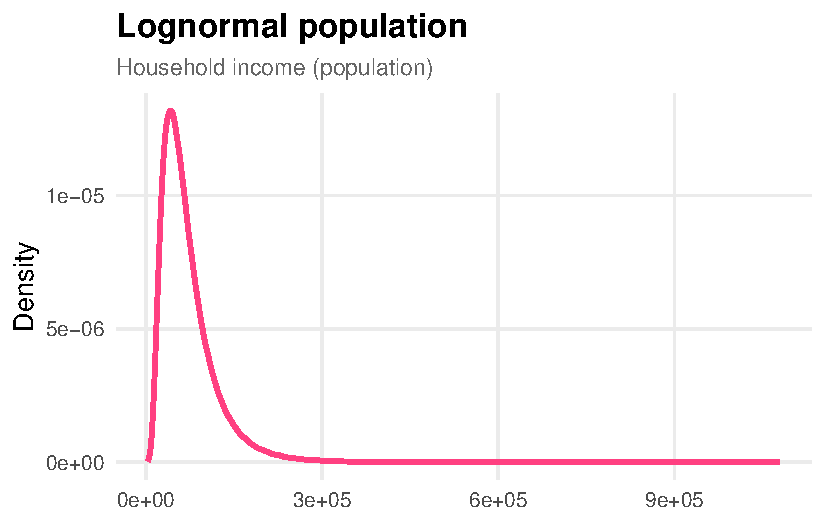
\includegraphics[keepaspectratio]{index_files/figure-pdf/unnamed-chunk-45-1.pdf}}

\pandocbounded{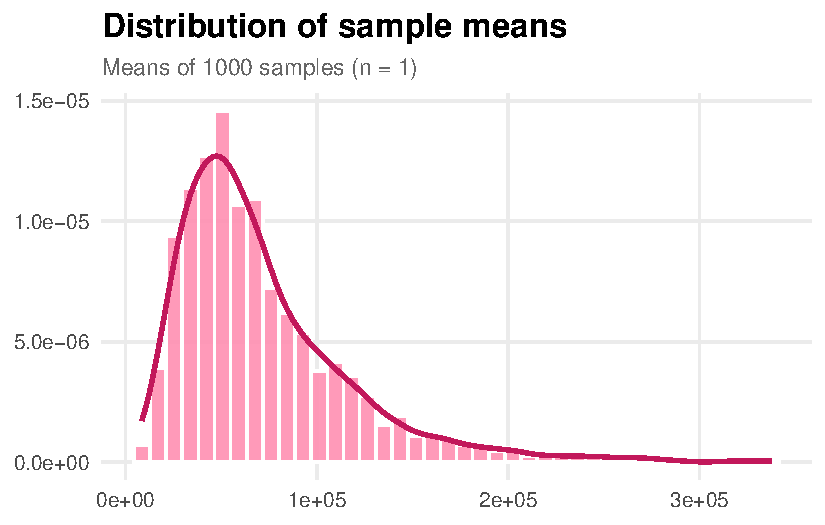
\includegraphics[keepaspectratio]{index_files/figure-pdf/unnamed-chunk-45-2.pdf}}

\pandocbounded{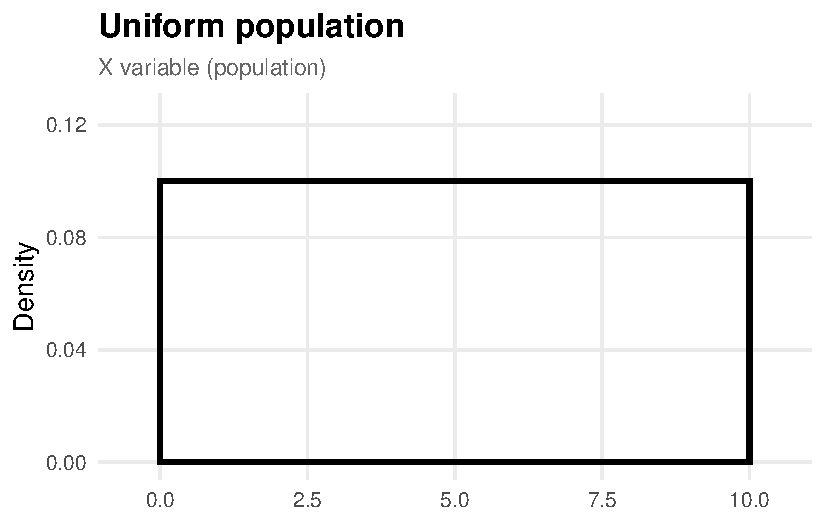
\includegraphics[keepaspectratio]{index_files/figure-pdf/unnamed-chunk-45-3.pdf}}

\pandocbounded{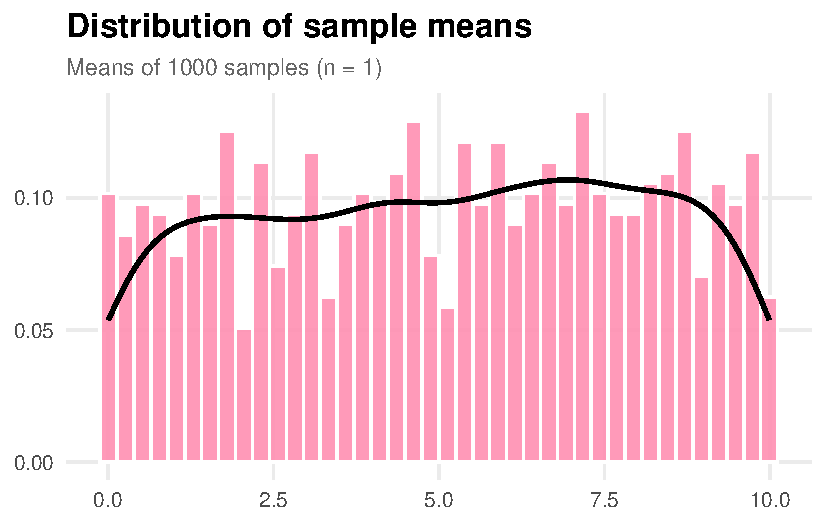
\includegraphics[keepaspectratio]{index_files/figure-pdf/unnamed-chunk-45-4.pdf}}

\section{Sampling Distributions from Other Populations ((n =
5))}\label{sampling-distributions-from-other-populations-n-5}

When the sample size increases, the \textbf{sampling distribution of the
mean} begins to look more Normal---even if the underlying population is
not.\\
Below we compare two populations: one \textbf{lognormal} (right-skewed)
and one \textbf{uniform} (flat).

For each, we repeatedly draw 1,000 random samples of size (n=5) and plot
the resulting means.\\
The lognormal sampling distribution still shows some skew, while the
uniform's mean distribution is already close to symmetric.

\begin{Shaded}
\begin{Highlighting}[]
\CommentTok{\#| echo: false}
\CommentTok{\#| message: false}
\CommentTok{\#| warning: false}
\CommentTok{\#| fig{-}width: 8}
\CommentTok{\#| fig{-}height: 6}
\CommentTok{\#| fig{-}cap: "Sampling distributions from lognormal and uniform populations (n = 5)."}
\CommentTok{\#| layout{-}ncol: 2}

\FunctionTok{library}\NormalTok{(ggplot2)}

\FunctionTok{set.seed}\NormalTok{(}\DecValTok{123}\NormalTok{)}

\CommentTok{\# {-}{-}{-}{-}{-}{-}{-}{-}{-}{-} Lognormal population {-}{-}{-}{-}{-}{-}{-}{-}{-}{-}}
\NormalTok{x\_lognorm }\OtherTok{\textless{}{-}} \FunctionTok{rlnorm}\NormalTok{(}\FloatTok{1e6}\NormalTok{, }\AttributeTok{meanlog =} \DecValTok{11}\NormalTok{, }\AttributeTok{sdlog =} \FloatTok{0.6}\NormalTok{)}
\NormalTok{means\_ln  }\OtherTok{\textless{}{-}} \FunctionTok{replicate}\NormalTok{(}\DecValTok{1000}\NormalTok{, }\FunctionTok{mean}\NormalTok{(}\FunctionTok{sample}\NormalTok{(x\_lognorm, }\DecValTok{5}\NormalTok{)))}

\NormalTok{p1 }\OtherTok{\textless{}{-}} \FunctionTok{ggplot}\NormalTok{(}\FunctionTok{data.frame}\NormalTok{(}\AttributeTok{x =}\NormalTok{ x\_lognorm), }\FunctionTok{aes}\NormalTok{(x)) }\SpecialCharTok{+}
  \FunctionTok{geom\_density}\NormalTok{(}\AttributeTok{color =} \StringTok{"\#FF4081"}\NormalTok{, }\AttributeTok{linewidth =} \FloatTok{1.1}\NormalTok{) }\SpecialCharTok{+}
  \FunctionTok{labs}\NormalTok{(}\AttributeTok{title =} \StringTok{"Lognormal population"}\NormalTok{,}
       \AttributeTok{subtitle =} \StringTok{"Household income (population)"}\NormalTok{,}
       \AttributeTok{x =} \ConstantTok{NULL}\NormalTok{, }\AttributeTok{y =} \StringTok{"Density"}\NormalTok{) }\SpecialCharTok{+}
  \FunctionTok{theme\_minimal}\NormalTok{(}\AttributeTok{base\_size =} \DecValTok{13}\NormalTok{) }\SpecialCharTok{+}
  \FunctionTok{theme}\NormalTok{(}\AttributeTok{plot.title =} \FunctionTok{element\_text}\NormalTok{(}\AttributeTok{face =} \StringTok{"bold"}\NormalTok{),}
        \AttributeTok{plot.subtitle =} \FunctionTok{element\_text}\NormalTok{(}\AttributeTok{size =} \DecValTok{11}\NormalTok{, }\AttributeTok{color =} \StringTok{"\#666"}\NormalTok{),}
        \AttributeTok{panel.grid.minor =} \FunctionTok{element\_blank}\NormalTok{(),}
        \AttributeTok{plot.background =} \FunctionTok{element\_rect}\NormalTok{(}\AttributeTok{fill =} \StringTok{"white"}\NormalTok{, }\AttributeTok{color =} \ConstantTok{NA}\NormalTok{))}

\NormalTok{p2 }\OtherTok{\textless{}{-}} \FunctionTok{ggplot}\NormalTok{(}\FunctionTok{data.frame}\NormalTok{(}\AttributeTok{x =}\NormalTok{ means\_ln), }\FunctionTok{aes}\NormalTok{(x)) }\SpecialCharTok{+}
  \FunctionTok{geom\_histogram}\NormalTok{(}\FunctionTok{aes}\NormalTok{(}\AttributeTok{y =} \FunctionTok{after\_stat}\NormalTok{(density)),}
                 \AttributeTok{bins =} \DecValTok{40}\NormalTok{, }\AttributeTok{fill =} \StringTok{"\#FF8FB1"}\NormalTok{, }\AttributeTok{color =} \StringTok{"white"}\NormalTok{, }\AttributeTok{alpha =} \FloatTok{0.9}\NormalTok{) }\SpecialCharTok{+}
  \FunctionTok{geom\_density}\NormalTok{(}\AttributeTok{color =} \StringTok{"\#C2185B"}\NormalTok{, }\AttributeTok{linewidth =} \DecValTok{1}\NormalTok{) }\SpecialCharTok{+}
  \FunctionTok{labs}\NormalTok{(}\AttributeTok{title =} \StringTok{"Distribution of sample means"}\NormalTok{,}
       \AttributeTok{subtitle =} \StringTok{"Means of 1000 samples (n = 5)"}\NormalTok{,}
       \AttributeTok{x =} \ConstantTok{NULL}\NormalTok{, }\AttributeTok{y =} \ConstantTok{NULL}\NormalTok{) }\SpecialCharTok{+}
  \FunctionTok{theme\_minimal}\NormalTok{(}\AttributeTok{base\_size =} \DecValTok{13}\NormalTok{) }\SpecialCharTok{+}
  \FunctionTok{theme}\NormalTok{(}\AttributeTok{plot.title =} \FunctionTok{element\_text}\NormalTok{(}\AttributeTok{face =} \StringTok{"bold"}\NormalTok{),}
        \AttributeTok{plot.subtitle =} \FunctionTok{element\_text}\NormalTok{(}\AttributeTok{size =} \DecValTok{11}\NormalTok{, }\AttributeTok{color =} \StringTok{"\#666"}\NormalTok{),}
        \AttributeTok{panel.grid.minor =} \FunctionTok{element\_blank}\NormalTok{(),}
        \AttributeTok{plot.background =} \FunctionTok{element\_rect}\NormalTok{(}\AttributeTok{fill =} \StringTok{"white"}\NormalTok{, }\AttributeTok{color =} \ConstantTok{NA}\NormalTok{))}


\CommentTok{\# {-}{-}{-}{-}{-}{-}{-}{-}{-}{-} Uniform population (rectangular + black lines) {-}{-}{-}{-}{-}{-}{-}{-}{-}{-}}
\NormalTok{a }\OtherTok{\textless{}{-}} \DecValTok{0}\NormalTok{; b }\OtherTok{\textless{}{-}} \DecValTok{10}\NormalTok{; h }\OtherTok{\textless{}{-}} \DecValTok{1}\SpecialCharTok{/}\NormalTok{(b }\SpecialCharTok{{-}}\NormalTok{ a)}
\NormalTok{x\_uniform }\OtherTok{\textless{}{-}} \FunctionTok{runif}\NormalTok{(}\FloatTok{1e6}\NormalTok{, a, b)}
\NormalTok{means\_unif }\OtherTok{\textless{}{-}} \FunctionTok{replicate}\NormalTok{(}\DecValTok{1000}\NormalTok{, }\FunctionTok{mean}\NormalTok{(}\FunctionTok{sample}\NormalTok{(x\_uniform, }\DecValTok{5}\NormalTok{)))}

\CommentTok{\# Uniform population (flat rectangle)}
\NormalTok{p3 }\OtherTok{\textless{}{-}} \FunctionTok{ggplot}\NormalTok{() }\SpecialCharTok{+}
  \FunctionTok{geom\_rect}\NormalTok{(}\FunctionTok{aes}\NormalTok{(}\AttributeTok{xmin =}\NormalTok{ a, }\AttributeTok{xmax =}\NormalTok{ b, }\AttributeTok{ymin =} \DecValTok{0}\NormalTok{, }\AttributeTok{ymax =}\NormalTok{ h),}
            \AttributeTok{fill =} \ConstantTok{NA}\NormalTok{, }\AttributeTok{color =} \StringTok{"black"}\NormalTok{, }\AttributeTok{linewidth =} \FloatTok{1.2}\NormalTok{) }\SpecialCharTok{+}
  \FunctionTok{scale\_x\_continuous}\NormalTok{(}\AttributeTok{limits =} \FunctionTok{c}\NormalTok{(a }\SpecialCharTok{{-}} \FloatTok{0.5}\NormalTok{, b }\SpecialCharTok{+} \FloatTok{0.5}\NormalTok{)) }\SpecialCharTok{+}
  \FunctionTok{scale\_y\_continuous}\NormalTok{(}\AttributeTok{limits =} \FunctionTok{c}\NormalTok{(}\DecValTok{0}\NormalTok{, h }\SpecialCharTok{*} \FloatTok{1.25}\NormalTok{)) }\SpecialCharTok{+}
  \FunctionTok{labs}\NormalTok{(}\AttributeTok{title =} \StringTok{"Uniform population"}\NormalTok{,}
       \AttributeTok{subtitle =} \StringTok{"X variable (population)"}\NormalTok{,}
       \AttributeTok{x =} \ConstantTok{NULL}\NormalTok{, }\AttributeTok{y =} \StringTok{"Density"}\NormalTok{) }\SpecialCharTok{+}
  \FunctionTok{theme\_minimal}\NormalTok{(}\AttributeTok{base\_size =} \DecValTok{13}\NormalTok{) }\SpecialCharTok{+}
  \FunctionTok{theme}\NormalTok{(}\AttributeTok{plot.title =} \FunctionTok{element\_text}\NormalTok{(}\AttributeTok{face =} \StringTok{"bold"}\NormalTok{),}
        \AttributeTok{plot.subtitle =} \FunctionTok{element\_text}\NormalTok{(}\AttributeTok{size =} \DecValTok{11}\NormalTok{, }\AttributeTok{color =} \StringTok{"\#666"}\NormalTok{),}
        \AttributeTok{panel.grid.minor =} \FunctionTok{element\_blank}\NormalTok{(),}
        \AttributeTok{plot.background =} \FunctionTok{element\_rect}\NormalTok{(}\AttributeTok{fill =} \StringTok{"white"}\NormalTok{, }\AttributeTok{color =} \ConstantTok{NA}\NormalTok{))}

\CommentTok{\# Uniform sampling distribution (pink hist, black line)}
\NormalTok{p4 }\OtherTok{\textless{}{-}} \FunctionTok{ggplot}\NormalTok{(}\FunctionTok{data.frame}\NormalTok{(}\AttributeTok{x =}\NormalTok{ means\_unif), }\FunctionTok{aes}\NormalTok{(x)) }\SpecialCharTok{+}
  \FunctionTok{geom\_histogram}\NormalTok{(}\FunctionTok{aes}\NormalTok{(}\AttributeTok{y =} \FunctionTok{after\_stat}\NormalTok{(density)),}
                 \AttributeTok{bins =} \DecValTok{40}\NormalTok{, }\AttributeTok{fill =} \StringTok{"\#FF8FB1"}\NormalTok{, }\AttributeTok{color =} \StringTok{"white"}\NormalTok{, }\AttributeTok{alpha =} \FloatTok{0.9}\NormalTok{) }\SpecialCharTok{+}
  \FunctionTok{geom\_density}\NormalTok{(}\AttributeTok{color =} \StringTok{"black"}\NormalTok{, }\AttributeTok{linewidth =} \DecValTok{1}\NormalTok{) }\SpecialCharTok{+}
  \FunctionTok{labs}\NormalTok{(}\AttributeTok{title =} \StringTok{"Distribution of sample means"}\NormalTok{,}
       \AttributeTok{subtitle =} \StringTok{"Means of 1000 samples (n = 5)"}\NormalTok{,}
       \AttributeTok{x =} \ConstantTok{NULL}\NormalTok{, }\AttributeTok{y =} \ConstantTok{NULL}\NormalTok{) }\SpecialCharTok{+}
  \FunctionTok{theme\_minimal}\NormalTok{(}\AttributeTok{base\_size =} \DecValTok{13}\NormalTok{) }\SpecialCharTok{+}
  \FunctionTok{theme}\NormalTok{(}\AttributeTok{plot.title =} \FunctionTok{element\_text}\NormalTok{(}\AttributeTok{face =} \StringTok{"bold"}\NormalTok{),}
        \AttributeTok{plot.subtitle =} \FunctionTok{element\_text}\NormalTok{(}\AttributeTok{size =} \DecValTok{11}\NormalTok{, }\AttributeTok{color =} \StringTok{"\#666"}\NormalTok{),}
        \AttributeTok{panel.grid.minor =} \FunctionTok{element\_blank}\NormalTok{(),}
        \AttributeTok{plot.background =} \FunctionTok{element\_rect}\NormalTok{(}\AttributeTok{fill =} \StringTok{"white"}\NormalTok{, }\AttributeTok{color =} \ConstantTok{NA}\NormalTok{))}

\CommentTok{\# Display 2×2 grid via layout{-}ncol}
\NormalTok{p1; p2; p3; p4}
\end{Highlighting}
\end{Shaded}

\pandocbounded{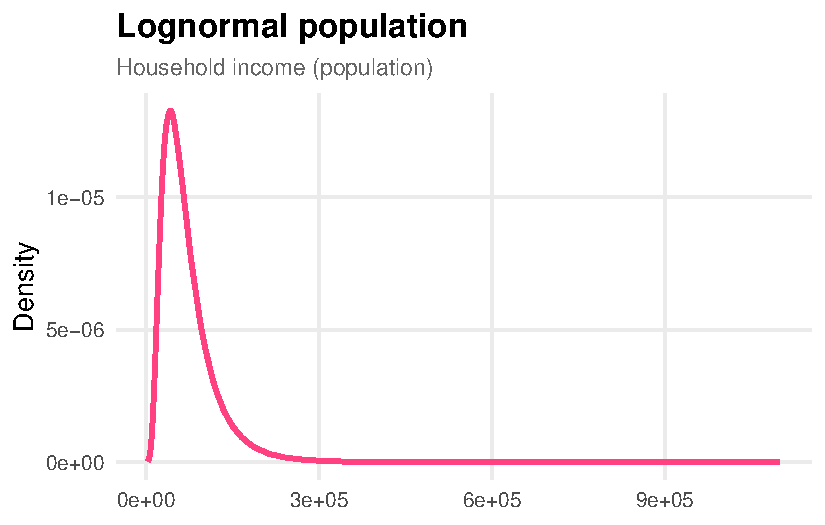
\includegraphics[keepaspectratio]{index_files/figure-pdf/unnamed-chunk-46-1.pdf}}

\pandocbounded{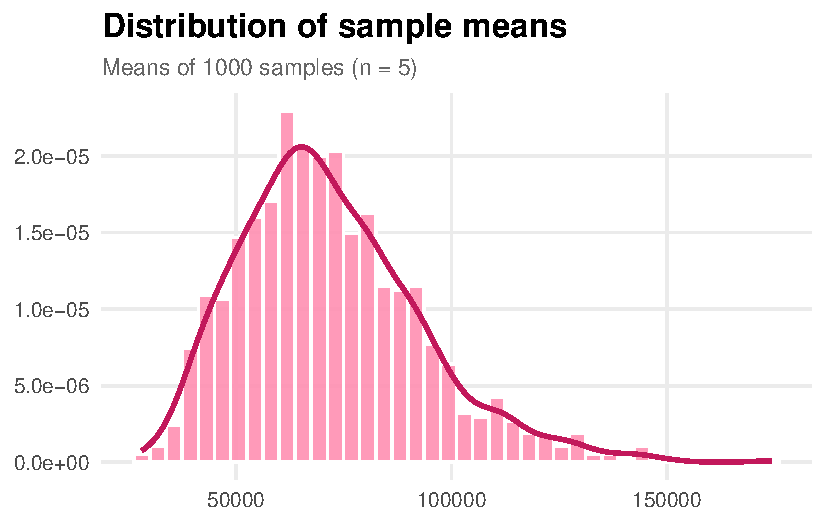
\includegraphics[keepaspectratio]{index_files/figure-pdf/unnamed-chunk-46-2.pdf}}

\pandocbounded{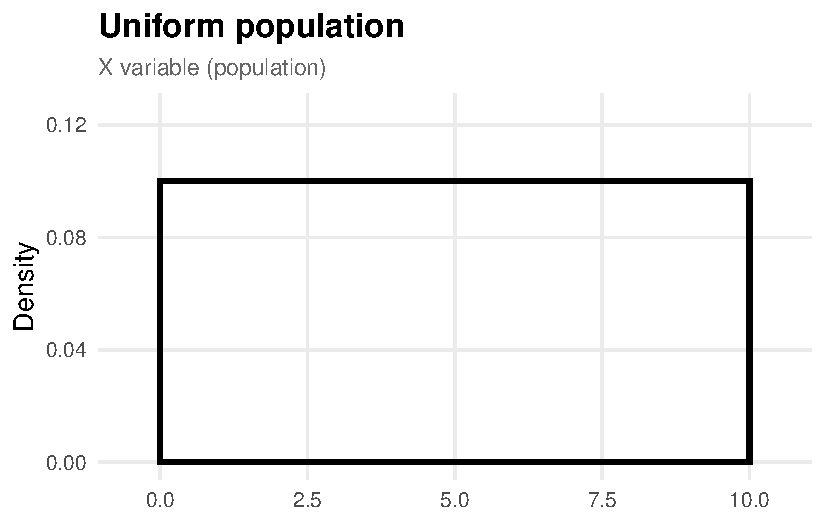
\includegraphics[keepaspectratio]{index_files/figure-pdf/unnamed-chunk-46-3.pdf}}

\pandocbounded{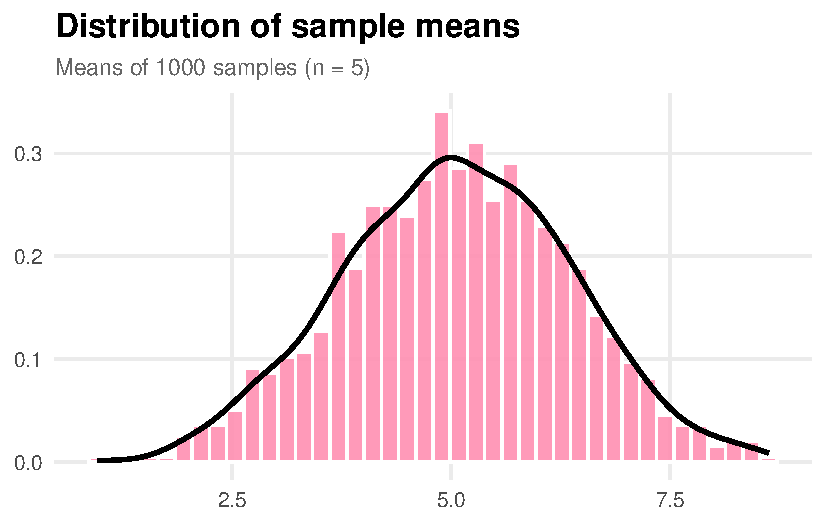
\includegraphics[keepaspectratio]{index_files/figure-pdf/unnamed-chunk-46-4.pdf}}

\section{Recap of Important Concepts}\label{recap-of-important-concepts}

\textbf{Sampling distributions} are theoretical, long-run probability
distributions.\\
They describe the distribution of the sample mean ( \bar\{X\} ) over all
possible samples of a given size ( n )---that is, what would happen if
we repeatedly took an infinite number of random samples of size ( n )
from the same population.

The \textbf{standard deviation of a sampling distribution}, also known
as the \emph{standard error of the mean}, depends on both the population
standard deviation ( \sigma ) and the sample size ( n ):

\[
\text{Standard deviation of sampling distribution} = \frac{\sigma}{\sqrt{n}}
\]

As the sample size ( n ) increases, the variability of the sampling
distribution decreases.\\
Larger samples produce means that cluster more tightly around the true
population mean ( \mu ).\\
This is a direct consequence of the \textbf{Law of Large Numbers (LLN)}:
with more observations, the sample mean becomes a more reliable
estimator of ( \mu ).

Because sampling distributions are \emph{theoretical}, their properties
depend only on ( n ) and on the characteristics of the underlying
population.\\
For each specific value of ( n ), the \textbf{shape}, \textbf{mean}, and
\textbf{standard deviation} of the sampling distribution are fixed---not
random.

\bookmarksetup{startatroot}

\chapter{Chapter 9: Confidence
Intervals}\label{chapter-9-confidence-intervals}

\section{Understanding the Concept of Confidence
Intervals}\label{understanding-the-concept-of-confidence-intervals}

In the previous chapter, we learned that \(\bar{x}\), the sample mean,
has a particular distribution in repeated samples, called its
\emph{sampling distribution}. Assuming a simple random sample is being
used, the sampling distribution of \(\bar{x}\) has a mean of \(\mu\),
the same numerical value as the population's mean. It also has a
standard deviation of \(\sigma/\sqrt{n}\). When \(n\) is large enough,
the distribution takes the Normal shape. Those are crucial facts, but
the usefulness of them comes when we consider how to interpret a
\emph{single} \(\bar{x}\) value from a \emph{single} sample. It turns
out we can use the facts about the sampling distribution to devise a
principled and reasonable way to make a guess about a range of values in
which we think the population mean lies, using only a \emph{single}
sample. This guess or estimate of a range for \(\mu\) is called a
\emph{confidence interval}.

Suppose we are interested in estimating the mean height of female
students at the University of Pennsylvania. We collect a sample of data
from female students enrolled in Social Statistics. Can we treat the
heights of these students as a random sample of the heights of all women
at the University of Pennsylvania? Strictly speaking, no, but for the
purpose of illustration, we will assume that we can.

Our sample size is \(n = 17\), and the sample mean is
\(\bar{x} = 64.82\). This value, \(\bar{x}\), serves as our estimate of
the population mean, \(\mu\), though we know it will not be exactly
correct. To express the uncertainty associated with this estimate, we
aim to construct an interval of plausible values for \(\mu\)---an
interval that, under repeated sampling, would contain the true mean a
specified proportion of the time. This is the basic idea behind a
confidence interval.

\begin{Shaded}
\begin{Highlighting}[]
\CommentTok{\#| echo: false}
\CommentTok{\#| message: false}
\CommentTok{\#| warning: false}

\CommentTok{\# {-}{-}{-}{-} data (base R only) {-}{-}{-}{-}}
\NormalTok{heights }\OtherTok{\textless{}{-}} \FunctionTok{data.frame}\NormalTok{(}
  \AttributeTok{student =} \FunctionTok{c}\NormalTok{(}\StringTok{"Emma C."}\NormalTok{,}\StringTok{"Tiana C."}\NormalTok{,}\StringTok{"Clare D."}\NormalTok{,}\StringTok{"Kristin G."}\NormalTok{,}\StringTok{"Kristin K."}\NormalTok{,}
              \StringTok{"Kendra K."}\NormalTok{,}\StringTok{"Beth K."}\NormalTok{,}\StringTok{"Natalie L."}\NormalTok{,}\StringTok{"Stephanie M."}\NormalTok{,}\StringTok{"Elizabeth P."}\NormalTok{,}
              \StringTok{"Alana P."}\NormalTok{,}\StringTok{"Cailey P."}\NormalTok{,}\StringTok{"Rhea S."}\NormalTok{,}\StringTok{"Laura S."}\NormalTok{,}\StringTok{"Ashley T."}\NormalTok{,}
              \StringTok{"Rachel W."}\NormalTok{,}\StringTok{"Marissa U."}\NormalTok{),}
  \AttributeTok{height  =} \FunctionTok{c}\NormalTok{(}\DecValTok{67}\NormalTok{,}\DecValTok{62}\NormalTok{,}\DecValTok{62}\NormalTok{,}\DecValTok{66}\NormalTok{,}\DecValTok{63}\NormalTok{,}\DecValTok{63}\NormalTok{,}\DecValTok{65}\NormalTok{,}\DecValTok{67}\NormalTok{,}\DecValTok{68}\NormalTok{,}\DecValTok{66}\NormalTok{,}\DecValTok{64}\NormalTok{,}\DecValTok{71}\NormalTok{,}\DecValTok{62}\NormalTok{,}\DecValTok{66}\NormalTok{,}\DecValTok{63}\NormalTok{,}\DecValTok{62}\NormalTok{,}\DecValTok{65}\NormalTok{),}
  \AttributeTok{stringsAsFactors =} \ConstantTok{FALSE}
\NormalTok{)}

\NormalTok{n\_obs }\OtherTok{\textless{}{-}} \FunctionTok{nrow}\NormalTok{(heights)}
\NormalTok{xbar  }\OtherTok{\textless{}{-}} \FunctionTok{mean}\NormalTok{(heights}\SpecialCharTok{$}\NormalTok{height)}

\CommentTok{\# Add row numbers as first column}
\NormalTok{heights }\OtherTok{\textless{}{-}} \FunctionTok{cbind}\NormalTok{(}\StringTok{\textasciigrave{}}\AttributeTok{\#}\StringTok{\textasciigrave{}} \OtherTok{=} \FunctionTok{seq\_len}\NormalTok{(n\_obs), heights)}

\CommentTok{\# {-}{-}{-}{-} print table with kable (knitr is built{-}in with Quarto) {-}{-}{-}{-}}
\NormalTok{knitr}\SpecialCharTok{::}\FunctionTok{kable}\NormalTok{(}
\NormalTok{  heights,}
  \AttributeTok{col.names =} \FunctionTok{c}\NormalTok{(}\StringTok{"\#"}\NormalTok{,}\StringTok{"Student"}\NormalTok{,}\StringTok{"Height (in)"}\NormalTok{),}
  \AttributeTok{align =} \FunctionTok{c}\NormalTok{(}\StringTok{"r"}\NormalTok{,}\StringTok{"l"}\NormalTok{,}\StringTok{"r"}\NormalTok{),}
  \AttributeTok{caption =} \FunctionTok{paste0}\NormalTok{(}\StringTok{"n = "}\NormalTok{, n\_obs, }\StringTok{";  x\textbackslash{}u0304 = "}\NormalTok{, }\FunctionTok{sprintf}\NormalTok{(}\StringTok{\textquotesingle{}\%.2f\textquotesingle{}}\NormalTok{, xbar))}
\NormalTok{)}
\end{Highlighting}
\end{Shaded}

\begin{longtable}[]{@{}rlr@{}}
\caption{n = 17; x̄ = 64.82}\tabularnewline
\toprule\noalign{}
\# & Student & Height (in) \\
\midrule\noalign{}
\endfirsthead
\toprule\noalign{}
\# & Student & Height (in) \\
\midrule\noalign{}
\endhead
\bottomrule\noalign{}
\endlastfoot
1 & Emma C. & 67 \\
2 & Tiana C. & 62 \\
3 & Clare D. & 62 \\
4 & Kristin G. & 66 \\
5 & Kristin K. & 63 \\
6 & Kendra K. & 63 \\
7 & Beth K. & 65 \\
8 & Natalie L. & 67 \\
9 & Stephanie M. & 68 \\
10 & Elizabeth P. & 66 \\
11 & Alana P. & 64 \\
12 & Cailey P. & 71 \\
13 & Rhea S. & 62 \\
14 & Laura S. & 66 \\
15 & Ashley T. & 63 \\
16 & Rachel W. & 62 \\
17 & Marissa U. & 65 \\
\end{longtable}

\begin{Shaded}
\begin{Highlighting}[]
\CommentTok{\#| echo: false}
\CommentTok{\#| message: false}
\CommentTok{\#| warning: false}
\CommentTok{\#| fig{-}width: 9}
\CommentTok{\#| fig{-}height: 5}
\CommentTok{\#| fig{-}cap: "Sampling distribution of \textbackslash{}\textbackslash{}(\textbackslash{}\textbackslash{}bar\{x\}\textbackslash{}\textbackslash{}) with 20 simulated 95\% confidence intervals; red dashed lines mark \textbackslash{}\textbackslash{}(\textbackslash{}\textbackslash{}mu\textbackslash{}\textbackslash{}pm1.31\textbackslash{}\textbackslash{})."}

\FunctionTok{library}\NormalTok{(ggplot2)}

\FunctionTok{set.seed}\NormalTok{(}\DecValTok{123}\NormalTok{)}

\CommentTok{\# {-}{-}{-} Parameters chosen so that 1.96*sigma/sqrt(n) = 1.31}
\NormalTok{mu    }\OtherTok{\textless{}{-}} \DecValTok{64}
\NormalTok{n     }\OtherTok{\textless{}{-}} \DecValTok{17}
\NormalTok{margin }\OtherTok{\textless{}{-}} \FloatTok{1.31}
\NormalTok{se    }\OtherTok{\textless{}{-}}\NormalTok{ margin }\SpecialCharTok{/} \FloatTok{1.96}               \CommentTok{\# standard error of xbar}
\NormalTok{sigma }\OtherTok{\textless{}{-}}\NormalTok{ se }\SpecialCharTok{*} \FunctionTok{sqrt}\NormalTok{(n)                 }\CommentTok{\# population sd consistent with margin}

\CommentTok{\# Simulate 20 samples, compute xbar and CIs using known sigma}
\NormalTok{M }\OtherTok{\textless{}{-}} \DecValTok{20}
\NormalTok{xbar   }\OtherTok{\textless{}{-}} \FunctionTok{replicate}\NormalTok{(M, }\FunctionTok{mean}\NormalTok{(}\FunctionTok{rnorm}\NormalTok{(n, }\AttributeTok{mean =}\NormalTok{ mu, }\AttributeTok{sd =}\NormalTok{ sigma)))}
\NormalTok{ci\_lo  }\OtherTok{\textless{}{-}}\NormalTok{ xbar }\SpecialCharTok{{-}}\NormalTok{ margin}
\NormalTok{ci\_hi  }\OtherTok{\textless{}{-}}\NormalTok{ xbar }\SpecialCharTok{+}\NormalTok{ margin}
\NormalTok{cover  }\OtherTok{\textless{}{-}}\NormalTok{ (ci\_lo }\SpecialCharTok{\textless{}=}\NormalTok{ mu) }\SpecialCharTok{\&}\NormalTok{ (ci\_hi }\SpecialCharTok{\textgreater{}=}\NormalTok{ mu)  }\CommentTok{\# does CI include the true mu?}

\NormalTok{df\_ci }\OtherTok{\textless{}{-}} \FunctionTok{data.frame}\NormalTok{(}
  \AttributeTok{id    =}\NormalTok{ M}\SpecialCharTok{:}\DecValTok{1}\NormalTok{,                 }\CommentTok{\# top to bottom ordering}
  \AttributeTok{xbar  =}\NormalTok{ xbar,}
  \AttributeTok{lo    =}\NormalTok{ ci\_lo,}
  \AttributeTok{hi    =}\NormalTok{ ci\_hi,}
  \AttributeTok{cover =}\NormalTok{ cover}
\NormalTok{)}

\CommentTok{\# Data for the xbar sampling density (Normal with mean mu and sd = se)}
\NormalTok{x\_grid }\OtherTok{\textless{}{-}} \FunctionTok{seq}\NormalTok{(}\DecValTok{60}\NormalTok{, }\DecValTok{68}\NormalTok{, }\AttributeTok{length.out =} \DecValTok{400}\NormalTok{)}
\NormalTok{dens   }\OtherTok{\textless{}{-}} \FunctionTok{dnorm}\NormalTok{(x\_grid, }\AttributeTok{mean =}\NormalTok{ mu, }\AttributeTok{sd =}\NormalTok{ se)}

\CommentTok{\# We\textquotesingle{}ll place the density in a "top band" by scaling its height}
\NormalTok{y\_top\_min }\OtherTok{\textless{}{-}}\NormalTok{ M }\SpecialCharTok{+} \DecValTok{3}
\NormalTok{y\_top\_max }\OtherTok{\textless{}{-}}\NormalTok{ M }\SpecialCharTok{+} \DecValTok{8}
\NormalTok{dens\_y }\OtherTok{\textless{}{-}}\NormalTok{ (dens }\SpecialCharTok{/} \FunctionTok{max}\NormalTok{(dens)) }\SpecialCharTok{*}\NormalTok{ (y\_top\_max }\SpecialCharTok{{-}}\NormalTok{ y\_top\_min) }\SpecialCharTok{+}\NormalTok{ y\_top\_min}
\NormalTok{df\_dens }\OtherTok{\textless{}{-}} \FunctionTok{data.frame}\NormalTok{(}\AttributeTok{x =}\NormalTok{ x\_grid, }\AttributeTok{y =}\NormalTok{ dens\_y)}

\CommentTok{\# Reference lines}
\NormalTok{left  }\OtherTok{\textless{}{-}}\NormalTok{ mu }\SpecialCharTok{{-}}\NormalTok{ margin}
\NormalTok{right }\OtherTok{\textless{}{-}}\NormalTok{ mu }\SpecialCharTok{+}\NormalTok{ margin}

\CommentTok{\# Build the composite plot in one ggplot}
\NormalTok{p }\OtherTok{\textless{}{-}} \FunctionTok{ggplot}\NormalTok{() }\SpecialCharTok{+}
  \CommentTok{\# {-}{-}{-} top density "panel"}
  \FunctionTok{geom\_rect}\NormalTok{(}\FunctionTok{aes}\NormalTok{(}\AttributeTok{xmin =} \DecValTok{60}\NormalTok{, }\AttributeTok{xmax =} \DecValTok{68}\NormalTok{, }\AttributeTok{ymin =}\NormalTok{ y\_top\_min, }\AttributeTok{ymax =}\NormalTok{ y\_top\_max),}
            \AttributeTok{fill =} \StringTok{"white"}\NormalTok{, }\AttributeTok{color =} \ConstantTok{NA}\NormalTok{) }\SpecialCharTok{+}
  \FunctionTok{geom\_line}\NormalTok{(}\AttributeTok{data =}\NormalTok{ df\_dens, }\FunctionTok{aes}\NormalTok{(x, y), }\AttributeTok{linewidth =} \DecValTok{1}\NormalTok{) }\SpecialCharTok{+}
  \FunctionTok{geom\_segment}\NormalTok{(}\FunctionTok{aes}\NormalTok{(}\AttributeTok{x =} \DecValTok{60}\NormalTok{, }\AttributeTok{xend =} \DecValTok{68}\NormalTok{, }\AttributeTok{y =}\NormalTok{ y\_top\_min, }\AttributeTok{yend =}\NormalTok{ y\_top\_min), }\AttributeTok{linewidth =} \FloatTok{0.6}\NormalTok{) }\SpecialCharTok{+}
  \FunctionTok{geom\_vline}\NormalTok{(}\AttributeTok{xintercept =}\NormalTok{ mu, }\AttributeTok{color =} \StringTok{"red1"}\NormalTok{, }\AttributeTok{linewidth =} \FloatTok{0.7}\NormalTok{) }\SpecialCharTok{+}
  \FunctionTok{geom\_vline}\NormalTok{(}\AttributeTok{xintercept =} \FunctionTok{c}\NormalTok{(left, right), }\AttributeTok{color =} \StringTok{"\#e74c3c"}\NormalTok{, }\AttributeTok{linetype =} \StringTok{"dashed"}\NormalTok{, }\AttributeTok{linewidth =} \FloatTok{0.7}\NormalTok{) }\SpecialCharTok{+}

  \CommentTok{\# {-}{-}{-} labels for 64±1.31}
  \FunctionTok{annotate}\NormalTok{(}\StringTok{"label"}\NormalTok{, }\AttributeTok{x =}\NormalTok{ left,  }\AttributeTok{y =}\NormalTok{ y\_top\_min }\SpecialCharTok{{-}} \FloatTok{0.7}\NormalTok{,}
           \AttributeTok{label =} \FunctionTok{paste0}\NormalTok{(}\StringTok{"64 {-} 1.31 = "}\NormalTok{, }\FunctionTok{sprintf}\NormalTok{(}\StringTok{"\%.2f"}\NormalTok{, left)),}
           \AttributeTok{size =} \FloatTok{3.6}\NormalTok{, }\AttributeTok{label.size =} \FloatTok{0.4}\NormalTok{, }\AttributeTok{fill =} \StringTok{"white"}\NormalTok{) }\SpecialCharTok{+}
  \FunctionTok{annotate}\NormalTok{(}\StringTok{"label"}\NormalTok{, }\AttributeTok{x =}\NormalTok{ right, }\AttributeTok{y =}\NormalTok{ y\_top\_min }\SpecialCharTok{{-}} \FloatTok{0.7}\NormalTok{,}
           \AttributeTok{label =} \FunctionTok{paste0}\NormalTok{(}\StringTok{"64 + 1.31 = "}\NormalTok{, }\FunctionTok{sprintf}\NormalTok{(}\StringTok{"\%.2f"}\NormalTok{, right)),}
           \AttributeTok{size =} \FloatTok{3.6}\NormalTok{, }\AttributeTok{label.size =} \FloatTok{0.4}\NormalTok{, }\AttributeTok{fill =} \StringTok{"white"}\NormalTok{) }\SpecialCharTok{+}

  \CommentTok{\# {-}{-}{-} bottom: 20 CIs (points are xbar; segments are intervals)}
  \FunctionTok{geom\_segment}\NormalTok{(}\AttributeTok{data =}\NormalTok{ df\_ci,}
               \FunctionTok{aes}\NormalTok{(}\AttributeTok{x =}\NormalTok{ lo, }\AttributeTok{xend =}\NormalTok{ hi, }\AttributeTok{y =}\NormalTok{ id, }\AttributeTok{yend =}\NormalTok{ id),}
               \AttributeTok{linewidth =} \FloatTok{0.9}\NormalTok{, }\AttributeTok{color =} \StringTok{"\#436EEE"}\NormalTok{) }\SpecialCharTok{+}
  \FunctionTok{geom\_point}\NormalTok{(}\AttributeTok{data =}\NormalTok{ df\_ci,}
             \FunctionTok{aes}\NormalTok{(}\AttributeTok{x =}\NormalTok{ xbar, }\AttributeTok{y =}\NormalTok{ id),}
             \AttributeTok{size =} \FloatTok{2.4}\NormalTok{, }\AttributeTok{color =} \StringTok{"\#FF4081"}\NormalTok{) }\SpecialCharTok{+}
  \CommentTok{\# vertical guides (same as top)}
  \FunctionTok{geom\_vline}\NormalTok{(}\AttributeTok{xintercept =}\NormalTok{ mu, }\AttributeTok{color =} \StringTok{"red4"}\NormalTok{, }\AttributeTok{linewidth =} \FloatTok{0.7}\NormalTok{) }\SpecialCharTok{+}
  \FunctionTok{geom\_vline}\NormalTok{(}\AttributeTok{xintercept =} \FunctionTok{c}\NormalTok{(left, right), }\AttributeTok{color =} \StringTok{"\#e74c3c"}\NormalTok{,}
             \AttributeTok{linetype =} \StringTok{"dashed"}\NormalTok{, }\AttributeTok{linewidth =} \FloatTok{0.7}\NormalTok{) }\SpecialCharTok{+}

  \CommentTok{\# {-}{-}{-} left{-}hand explanatory text (placed with annotate)}
  \FunctionTok{annotate}\NormalTok{(}\StringTok{"text"}\NormalTok{, }\AttributeTok{x =} \FloatTok{60.2}\NormalTok{, }\AttributeTok{y =}\NormalTok{ (y\_top\_min }\SpecialCharTok{+}\NormalTok{ y\_top\_max)}\SpecialCharTok{/}\DecValTok{2}\NormalTok{,}
           \AttributeTok{label =} \StringTok{"Sampling distribution}\SpecialCharTok{\textbackslash{}n}\StringTok{of x{-}bar values"}\NormalTok{,}
           \AttributeTok{hjust =} \DecValTok{0}\NormalTok{, }\AttributeTok{size =} \FloatTok{5.2}\NormalTok{) }\SpecialCharTok{+}
  \FunctionTok{annotate}\NormalTok{(}\StringTok{"text"}\NormalTok{, }\AttributeTok{x =} \FloatTok{60.2}\NormalTok{, }\AttributeTok{y =}\NormalTok{ M}\SpecialCharTok{/}\DecValTok{2}\NormalTok{,}
           \AttributeTok{label =} \StringTok{"Draws of x{-}bar values}\SpecialCharTok{\textbackslash{}n}\StringTok{with their constructed}\SpecialCharTok{\textbackslash{}n}\StringTok{95\% confidence}\SpecialCharTok{\textbackslash{}n}\StringTok{intervals"}\NormalTok{,}
           \AttributeTok{hjust =} \DecValTok{0}\NormalTok{, }\AttributeTok{size =} \FloatTok{5.2}\NormalTok{) }\SpecialCharTok{+}

  \CommentTok{\# Axes and theme}
  \FunctionTok{scale\_x\_continuous}\NormalTok{(}\AttributeTok{limits =} \FunctionTok{c}\NormalTok{(}\DecValTok{60}\NormalTok{, }\DecValTok{68}\NormalTok{), }\AttributeTok{breaks =} \FunctionTok{seq}\NormalTok{(}\DecValTok{60}\NormalTok{, }\DecValTok{68}\NormalTok{, }\AttributeTok{by =} \DecValTok{2}\NormalTok{)) }\SpecialCharTok{+}
  \FunctionTok{scale\_y\_continuous}\NormalTok{(}\ConstantTok{NULL}\NormalTok{, }\AttributeTok{breaks =} \ConstantTok{NULL}\NormalTok{) }\SpecialCharTok{+}
  \FunctionTok{labs}\NormalTok{(}\AttributeTok{x =} \ConstantTok{NULL}\NormalTok{, }\AttributeTok{y =} \ConstantTok{NULL}\NormalTok{) }\SpecialCharTok{+}
  \FunctionTok{theme\_minimal}\NormalTok{(}\AttributeTok{base\_size =} \DecValTok{13}\NormalTok{) }\SpecialCharTok{+}
  \FunctionTok{theme}\NormalTok{(}
    \AttributeTok{panel.grid =} \FunctionTok{element\_blank}\NormalTok{(),}
    \AttributeTok{plot.background =} \FunctionTok{element\_rect}\NormalTok{(}\AttributeTok{fill =} \StringTok{"white"}\NormalTok{, }\AttributeTok{color =} \ConstantTok{NA}\NormalTok{),}
    \AttributeTok{axis.text.x =} \FunctionTok{element\_text}\NormalTok{(}\AttributeTok{color =} \StringTok{"black"}\NormalTok{)}
\NormalTok{  )}

\NormalTok{p}
\end{Highlighting}
\end{Shaded}

\pandocbounded{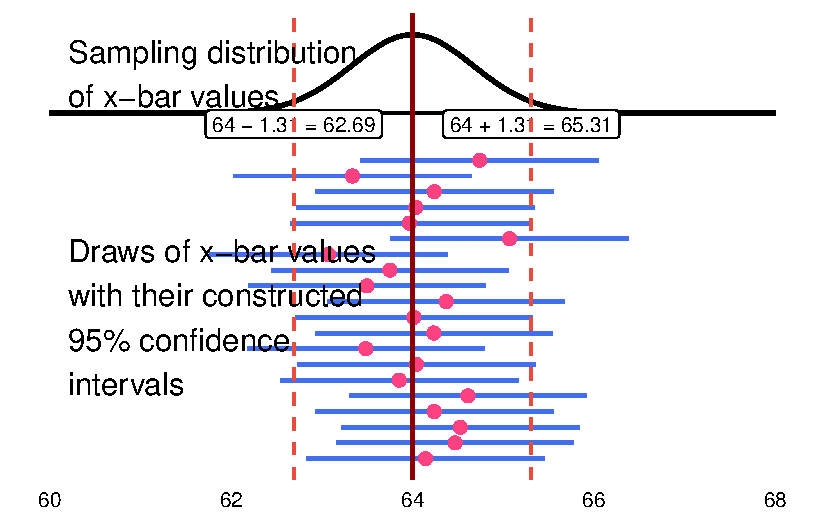
\includegraphics[keepaspectratio]{index_files/figure-pdf/unnamed-chunk-48-1.pdf}}

This is the calculation of exact 95\% confidence interval limits,
\emph{done around the sample mean} of 64.82:

\[
\begin{align}
95\%\text{CI} &= \bar{x} \pm z^* \frac{\sigma}{\sqrt{n}} \\
&= 64.82 \pm 1.96 \frac{2.7}{\sqrt{17}} \\
&= 64.82 \pm 1.96(.655) \\
&= (63.54, 66.10)
\end{align}
\]

I will now add this confidence interval to the earlier illustration of
the sampling distribution of confidence intervals.We happen to have
gotten a confidence interval that \emph{does} include \(\mu\). This
should happen 95\% of the time, and \emph{not happen} 5\% of the time.

\subsection{\texorpdfstring{The Impact of \(\sigma\), the Population
Standard
Deviation}{The Impact of \textbackslash sigma, the Population Standard Deviation}}\label{the-impact-of-sigma-the-population-standard-deviation}

The margin of error \(m\) is directly proportional to \(\sigma\), the
population standard deviation. This relationship is expressed
mathematically as:

\[
m = z^* \frac{\sigma}{\sqrt{n}}
\]

where:

\begin{itemize}
\tightlist
\item
  \(m\) is the margin of error
\item
  \(z^*\) is the critical value from the standard normal distribution
\item
  \(\sigma\) is the population standard deviation
\item
  \(n\) is the sample size
\end{itemize}

\subsection{Key implications of this
formula}\label{key-implications-of-this-formula}

The larger the population standard deviation \(\sigma\), the larger
(wider) the margin of error becomes, which in turn produces a wider
confidence interval. This makes intuitive sense: when there is more
variability in the population, our estimates are naturally less precise.

There is nothing the researcher can do about \(\sigma\), as a general
rule. The population standard deviation is a fixed characteristic of the
population being studied and exists independently of the researcher's
choices.

This makes \(\sigma\) fundamentally different from \(z^*\) and \(n\),
both of which are under the researcher's control. The researcher chooses
the confidence level (which determines \(z^*\)) and the sample size
\(n\).

However, neither \(z^*\) nor \(n\) amount to a ``free lunch'' as a means
of controlling the margin of error:

\begin{itemize}
\item
  \(z^*\) can only be decreased by decreasing the confidence level
  \(C\). In other words, to achieve a smaller margin of error through
  \(z^*\), the researcher must accept less confidence in the resulting
  interval. This represents a direct tradeoff between precision and
  certainty.
\item
  Increasing the sample size \(n\) takes more money. Larger samples
  require more resources, time, and funding to collect. While this
  approach does reduce the margin of error (note that \(n\) appears in
  the denominator under a square root), the improvement comes at a real
  financial cost.
\end{itemize}

\bookmarksetup{startatroot}

\chapter{Chapter 10: Test of
Significance}\label{chapter-10-test-of-significance}

There are two closely related methods for drawing inferences about
population parameters.A confidence interval uses information from a
sample to estimate a plausible range of values for the population
parameter. A significance test, by contrast, evaluates a specific claim
or assertion about that parameter using the same sample data. The claim
being tested is known as a hypothesis, which must be clearly formulated
and expressed in formal mathematical notation.

\section{The reasoning in tests of
significance:}\label{the-reasoning-in-tests-of-significance}

\subsection{Example:}\label{example}

Suppose that a researcher claims that a new civic education program
increases voter turnout by 10 percentage points compared to areas
without the program.You are skeptical and believe the program might have
little or no effect. To test this claim, you collect data from 20
communities that implemented the program and find that, on average,
turnout increased by only 2 percentage points.

What does this suggest about the researcher's claim? Your (likely)
reasoning follows the same logic as a significance test:

☞ If I assume the researcher's claim is correct (that the true increase
is 10 percentage points), then observing only a 2-point increase would
be highly unexpected.

☞ Therefore, I reject the claim and conclude that the evidence does not
support such a large program effect.This mirrors the structure of
hypothesis testing: we begin by assuming the claim (the null
hypothesis), examine how surprising our data are under that assumption,
and---if the results are too unlikely---decide that the claim is
probably false.

\section{Using the Binomial
Distribution}\label{using-the-binomial-distribution}

For testing a civic education program's impact on voter turnout, the
\emph{binomial distribution} provides a useful framework:

\begin{itemize}
\tightlist
\item
  The communities are independent
\item
  \(p = 0.10\) is the claimed increase in turnout (10 percentage points)
\item
  There are \(n = 20\) communities in the study
\end{itemize}

We can examine the distribution to understand the probability of
observing only 2 communities (or fewer) showing the claimed
10-percentage-point increase, if the researcher's claim were true.

Evidently, that probability is extremely small---close to zero.

This strongly suggests the researcher's claim is false.

\begin{Shaded}
\begin{Highlighting}[]
\CommentTok{\#| echo: false}
\CommentTok{\#| message: false}
\CommentTok{\#| warning: false}
\CommentTok{\#| fig{-}width: 9}
\CommentTok{\#| fig{-}height: 5.5}
\CommentTok{\#| fig{-}cap: "Probability mass function for daily coffee consumption among US adults (n = 2,847)."}

\FunctionTok{suppressPackageStartupMessages}\NormalTok{(\{}
  \FunctionTok{library}\NormalTok{(ggplot2); }\FunctionTok{library}\NormalTok{(dplyr); }\FunctionTok{library}\NormalTok{(scales)}
\NormalTok{\})}

\CommentTok{\# PMF for cups of coffee per day}
\NormalTok{df }\OtherTok{\textless{}{-}} \FunctionTok{data.frame}\NormalTok{(}
  \AttributeTok{cups =} \DecValTok{0}\SpecialCharTok{:}\DecValTok{5}\NormalTok{,}
  \AttributeTok{cups\_label =} \FunctionTok{c}\NormalTok{(}\StringTok{"0"}\NormalTok{,}\StringTok{"1"}\NormalTok{,}\StringTok{"2"}\NormalTok{,}\StringTok{"3"}\NormalTok{,}\StringTok{"4"}\NormalTok{,}\StringTok{"≥5"}\NormalTok{),}
  \AttributeTok{probability =} \FunctionTok{c}\NormalTok{(}\FloatTok{0.18}\NormalTok{, }\FloatTok{0.24}\NormalTok{, }\FloatTok{0.31}\NormalTok{, }\FloatTok{0.16}\NormalTok{, }\FloatTok{0.07}\NormalTok{, }\FloatTok{0.04}\NormalTok{)}
\NormalTok{) }\SpecialCharTok{\%\textgreater{}\%}
  \FunctionTok{mutate}\NormalTok{(}
    \AttributeTok{intensity =}\NormalTok{ probability }\SpecialCharTok{/} \FunctionTok{max}\NormalTok{(probability)}
\NormalTok{  )}

\CommentTok{\# Calculate mean for annotation}
\NormalTok{expected\_value }\OtherTok{\textless{}{-}} \FunctionTok{sum}\NormalTok{(df}\SpecialCharTok{$}\NormalTok{cups }\SpecialCharTok{*}\NormalTok{ df}\SpecialCharTok{$}\NormalTok{probability)}

\FunctionTok{ggplot}\NormalTok{(df, }\FunctionTok{aes}\NormalTok{(}\AttributeTok{x =}\NormalTok{ cups, }\AttributeTok{y =}\NormalTok{ probability)) }\SpecialCharTok{+}
  \FunctionTok{geom\_col}\NormalTok{(}
    \FunctionTok{aes}\NormalTok{(}\AttributeTok{fill =}\NormalTok{ intensity),}
    \AttributeTok{width =} \FloatTok{0.45}\NormalTok{,}
    \AttributeTok{color =} \StringTok{"white"}\NormalTok{,}
    \AttributeTok{linewidth =} \DecValTok{1}
\NormalTok{  ) }\SpecialCharTok{+}
  \FunctionTok{scale\_fill\_viridis\_c}\NormalTok{(}
    \AttributeTok{option =} \StringTok{"plasma"}\NormalTok{,}
    \AttributeTok{begin =} \FloatTok{0.2}\NormalTok{,}
    \AttributeTok{end =} \FloatTok{0.95}\NormalTok{,}
    \AttributeTok{guide =} \StringTok{"none"}
\NormalTok{  ) }\SpecialCharTok{+}
  \FunctionTok{geom\_text}\NormalTok{(}
    \FunctionTok{aes}\NormalTok{(}\AttributeTok{label =} \FunctionTok{percent}\NormalTok{(probability, }\AttributeTok{accuracy =} \DecValTok{1}\NormalTok{)),}
    \AttributeTok{vjust =} \SpecialCharTok{{-}}\FloatTok{0.7}\NormalTok{,}
    \AttributeTok{size =} \FloatTok{4.5}\NormalTok{,}
    \AttributeTok{fontface =} \StringTok{"bold"}\NormalTok{,}
    \AttributeTok{color =} \StringTok{"gray20"}
\NormalTok{  ) }\SpecialCharTok{+}
  \FunctionTok{annotate}\NormalTok{(}
    \StringTok{"curve"}\NormalTok{,}
    \AttributeTok{x =} \FloatTok{3.5}\NormalTok{, }\AttributeTok{xend =} \FloatTok{2.1}\NormalTok{,}
    \AttributeTok{y =} \FloatTok{0.35}\NormalTok{, }\AttributeTok{yend =} \FloatTok{0.32}\NormalTok{,}
    \AttributeTok{arrow =} \FunctionTok{arrow}\NormalTok{(}\AttributeTok{length =} \FunctionTok{unit}\NormalTok{(}\FloatTok{0.3}\NormalTok{, }\StringTok{"cm"}\NormalTok{), }\AttributeTok{type =} \StringTok{"closed"}\NormalTok{),}
    \AttributeTok{curvature =} \FloatTok{0.3}\NormalTok{,}
    \AttributeTok{linewidth =} \DecValTok{1}\NormalTok{,}
    \AttributeTok{color =} \StringTok{"\#BD3786"}
\NormalTok{  ) }\SpecialCharTok{+}
  \FunctionTok{annotate}\NormalTok{(}
    \StringTok{"text"}\NormalTok{,}
    \AttributeTok{x =} \FloatTok{3.8}\NormalTok{, }\AttributeTok{y =} \FloatTok{0.35}\NormalTok{,}
    \AttributeTok{label =} \StringTok{"Modal response:}\SpecialCharTok{\textbackslash{}n}\StringTok{2 cups per day"}\NormalTok{,}
    \AttributeTok{hjust =} \DecValTok{0}\NormalTok{,}
    \AttributeTok{size =} \FloatTok{2.4}\NormalTok{,}
    \AttributeTok{fontface =} \StringTok{"bold"}\NormalTok{,}
    \AttributeTok{color =} \StringTok{"\#BD3786"}\NormalTok{,}
    \AttributeTok{lineheight =} \FloatTok{0.9}
\NormalTok{  ) }\SpecialCharTok{+}
  \FunctionTok{annotate}\NormalTok{(}
    \StringTok{"text"}\NormalTok{,}
    \AttributeTok{x =} \FloatTok{0.3}\NormalTok{, }\AttributeTok{y =} \FloatTok{0.33}\NormalTok{,}
    \AttributeTok{label =} \FunctionTok{sprintf}\NormalTok{(}\StringTok{"Mean = \%.2f cups"}\NormalTok{, expected\_value),}
    \AttributeTok{hjust =} \DecValTok{0}\NormalTok{,}
    \AttributeTok{size =} \FloatTok{2.4}\NormalTok{,}
    \AttributeTok{fontface =} \StringTok{"italic"}\NormalTok{,}
    \AttributeTok{color =} \StringTok{"gray30"}
\NormalTok{  ) }\SpecialCharTok{+}
  \FunctionTok{scale\_x\_continuous}\NormalTok{(}
    \AttributeTok{breaks =} \DecValTok{0}\SpecialCharTok{:}\DecValTok{5}\NormalTok{,}
    \AttributeTok{labels =} \FunctionTok{c}\NormalTok{(}\StringTok{"0"}\NormalTok{,}\StringTok{"1"}\NormalTok{,}\StringTok{"2"}\NormalTok{,}\StringTok{"3"}\NormalTok{,}\StringTok{"4"}\NormalTok{,}\StringTok{"≥5"}\NormalTok{),}
    \AttributeTok{expand =} \FunctionTok{expansion}\NormalTok{(}\AttributeTok{mult =} \FunctionTok{c}\NormalTok{(}\FloatTok{0.05}\NormalTok{, }\FloatTok{0.05}\NormalTok{))}
\NormalTok{  ) }\SpecialCharTok{+}
  \FunctionTok{scale\_y\_continuous}\NormalTok{(}
    \AttributeTok{labels =} \FunctionTok{percent\_format}\NormalTok{(}\AttributeTok{accuracy =} \DecValTok{1}\NormalTok{),}
    \AttributeTok{limits =} \FunctionTok{c}\NormalTok{(}\DecValTok{0}\NormalTok{, }\FloatTok{0.39}\NormalTok{),}
    \AttributeTok{expand =} \FunctionTok{expansion}\NormalTok{(}\AttributeTok{mult =} \FunctionTok{c}\NormalTok{(}\DecValTok{0}\NormalTok{, }\DecValTok{0}\NormalTok{))}
\NormalTok{  ) }\SpecialCharTok{+}
  \FunctionTok{labs}\NormalTok{(}
    \AttributeTok{title =} \StringTok{"Americans Drink 2 Cups of Coffee Per Day, On Average"}\NormalTok{,}
    \AttributeTok{subtitle =} \StringTok{"Distribution of self{-}reported daily coffee consumption | Survey of 2,847 US adults"}\NormalTok{,}
    \AttributeTok{x =} \StringTok{"Daily Coffee Consumption (Cups)"}\NormalTok{,}
    \AttributeTok{y =} \StringTok{"Proportion of Respondents"}
\NormalTok{  ) }\SpecialCharTok{+}
  \FunctionTok{theme\_minimal}\NormalTok{(}\AttributeTok{base\_size =} \DecValTok{14}\NormalTok{) }\SpecialCharTok{+}
  \FunctionTok{theme}\NormalTok{(}
    \AttributeTok{plot.title =} \FunctionTok{element\_text}\NormalTok{(}\AttributeTok{face =} \StringTok{"bold"}\NormalTok{, }\AttributeTok{size =} \DecValTok{18}\NormalTok{, }\AttributeTok{hjust =} \DecValTok{0}\NormalTok{, }\AttributeTok{margin =} \FunctionTok{margin}\NormalTok{(}\AttributeTok{b =} \DecValTok{8}\NormalTok{), }\AttributeTok{color =} \StringTok{"gray10"}\NormalTok{),}
    \AttributeTok{plot.subtitle =} \FunctionTok{element\_text}\NormalTok{(}\AttributeTok{size =} \DecValTok{11}\NormalTok{, }\AttributeTok{color =} \StringTok{"gray40"}\NormalTok{, }\AttributeTok{hjust =} \DecValTok{0}\NormalTok{, }\AttributeTok{margin =} \FunctionTok{margin}\NormalTok{(}\AttributeTok{b =} \DecValTok{20}\NormalTok{)),}
    \AttributeTok{axis.title.x =} \FunctionTok{element\_text}\NormalTok{(}\AttributeTok{face =} \StringTok{"bold"}\NormalTok{, }\AttributeTok{size =} \DecValTok{13}\NormalTok{, }\AttributeTok{margin =} \FunctionTok{margin}\NormalTok{(}\AttributeTok{t =} \DecValTok{12}\NormalTok{), }\AttributeTok{color =} \StringTok{"gray20"}\NormalTok{),}
    \AttributeTok{axis.title.y =} \FunctionTok{element\_text}\NormalTok{(}\AttributeTok{face =} \StringTok{"bold"}\NormalTok{, }\AttributeTok{size =} \DecValTok{13}\NormalTok{, }\AttributeTok{margin =} \FunctionTok{margin}\NormalTok{(}\AttributeTok{r =} \DecValTok{12}\NormalTok{), }\AttributeTok{color =} \StringTok{"gray20"}\NormalTok{),}
    \AttributeTok{axis.text =} \FunctionTok{element\_text}\NormalTok{(}\AttributeTok{size =} \DecValTok{12}\NormalTok{, }\AttributeTok{color =} \StringTok{"gray30"}\NormalTok{),}
    \AttributeTok{panel.grid =} \FunctionTok{element\_blank}\NormalTok{(),}
    \AttributeTok{plot.background =} \FunctionTok{element\_rect}\NormalTok{(}\AttributeTok{fill =} \StringTok{"white"}\NormalTok{, }\AttributeTok{color =} \ConstantTok{NA}\NormalTok{),}
    \AttributeTok{panel.background =} \FunctionTok{element\_rect}\NormalTok{(}\AttributeTok{fill =} \StringTok{"white"}\NormalTok{, }\AttributeTok{color =} \ConstantTok{NA}\NormalTok{),}
    \AttributeTok{plot.margin =} \FunctionTok{margin}\NormalTok{(}\DecValTok{20}\NormalTok{, }\DecValTok{25}\NormalTok{, }\DecValTok{15}\NormalTok{, }\DecValTok{15}\NormalTok{),}
    \AttributeTok{axis.line =} \FunctionTok{element\_line}\NormalTok{(}\AttributeTok{color =} \StringTok{"gray50"}\NormalTok{, }\AttributeTok{linewidth =} \FloatTok{0.5}\NormalTok{)}
\NormalTok{  )}
\end{Highlighting}
\end{Shaded}

\pandocbounded{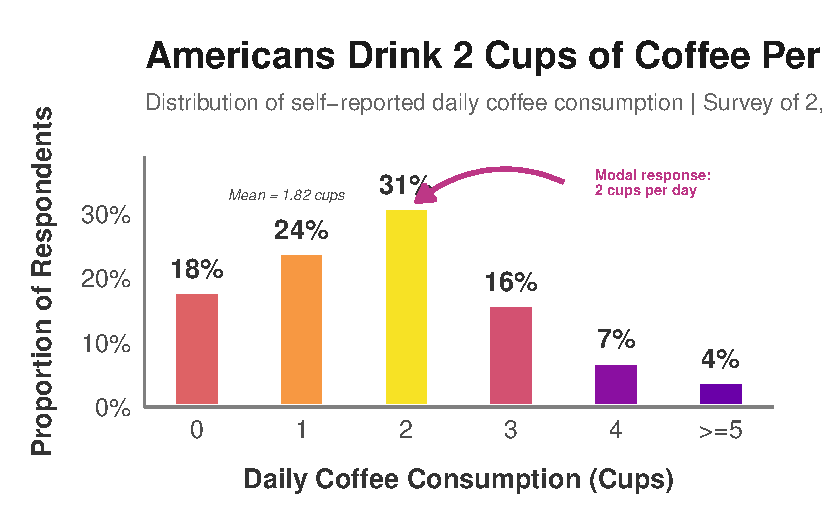
\includegraphics[keepaspectratio]{index_files/figure-pdf/unnamed-chunk-49-1.pdf}}

\subsection{Your (Likely) Reasoning}\label{your-likely-reasoning}

This follows the same logic as a significance test:

\textbf{If I assume the researcher's claim is correct} (that the true
increase is 10 percentage points in each community), then observing only
2 communities (or fewer) with such an increase out of 20 would be highly
unexpected---occurring with probability 0.6769.

\textbf{Therefore, I reject the claim} and conclude that the evidence
does not support such a large program effect.

This mirrors the structure of hypothesis testing: we begin by assuming
the claim (the null hypothesis), examine how surprising our data are
under that assumption, and---if the results are too unlikely---decide
that the claim is probably false.

\section{The Logic of Significance
Testing}\label{the-logic-of-significance-testing}

Statistical inference allows us to evaluate claims about population
parameters by examining how consistent our data are with those claims.
Suppose, for example, we claim that the probability of success in a task
is \(p = 0.8\). If, after repeated trials, we observe results far worse
than what would ordinarily occur under that assumption, it becomes
increasingly implausible that our claim is true. For instance, if the
chance of obtaining such poor results is extremely small---say, a
binomial probability of 0.0001---then those results constitute strong
evidence against the original claim.

A low probability of observing our data under a given assumption is good
evidence against that assumption, often called the \textbf{null
hypothesis}. When such evidence accumulates, we may reasonably conclude
that the null hypothesis is likely incorrect.

The logic of significance testing follows a simple but powerful
structure:

\begin{enumerate}
\def\labelenumi{\arabic{enumi}.}
\item
  \textbf{Formulate a claim to be tested}, known as the null hypothesis
  (\(H_0\)).
\item
  \textbf{Specify an alternative hypothesis} (\(H_1\)) that represents
  what we might believe if the null were false.
\item
  \textbf{Evaluate the data} under the assumption that the null
  hypothesis is true.
\item
  \textbf{Assess how unusual our results would be} if \(H_0\) were
  correct.

  \begin{itemize}
  \tightlist
  \item
    If the results would rarely occur by chance alone, we interpret them
    as evidence against \(H_0\) and in favor of \(H_1\).
  \end{itemize}
\end{enumerate}

In applied research, most tests rely on the Normal distribution (or its
close relatives) to approximate sampling variation. We therefore focus
on cases where this approximation provides a valid and interpretable
framework for decision-making.

\section{The Structure of Hypotheses}\label{the-structure-of-hypotheses}

Statistical inference allows us to evaluate claims about population
parameters by examining how consistent our data are with those claims.
Suppose, for example, we claim that the probability of success in a task
is \(p = 0.8\). If, after repeated trials, we observe results far worse
than what would ordinarily occur under that assumption, it becomes
increasingly implausible that our claim is true. For instance, if the
chance of obtaining such poor results is extremely small---say, a
binomial probability of 0.0001---then those results constitute strong
evidence against the original claim.

A low probability of observing our data under a given assumption is good
evidence against that assumption, often called the \textbf{null
hypothesis}. When such evidence accumulates, we may reasonably conclude
that the null hypothesis is likely incorrect.

\subsection{The Logic of Significance
Testing}\label{the-logic-of-significance-testing-1}

The logic of significance testing follows a simple but powerful
structure:

\begin{enumerate}
\def\labelenumi{\arabic{enumi}.}
\item
  \textbf{Formulate a claim to be tested}, known as the null hypothesis
  (\(H_0\)).
\item
  \textbf{Specify an alternative hypothesis} (\(H_1\)) that represents
  what we might believe if the null were false.
\item
  \textbf{Evaluate the data} under the assumption that the null
  hypothesis is true.
\item
  \textbf{Assess how unusual our results would be} if \(H_0\) were
  correct.

  \begin{itemize}
  \tightlist
  \item
    If the results would rarely occur by chance alone, we interpret them
    as evidence against \(H_0\) and in favor of \(H_1\).
  \end{itemize}
\end{enumerate}

In applied research, most tests rely on the Normal distribution (or its
close relatives) to approximate sampling variation. We therefore focus
on cases where this approximation provides a valid and interpretable
framework for decision-making.

\section{Historical Development of Hypothesis
Testing}\label{historical-development-of-hypothesis-testing}

Hypothesis testing as a formal method in statistics emerged in the early
twentieth century, shaped by three key figures---Ronald A. Fisher, Jerzy
Neyman, and Egon Pearson---whose distinct contributions gradually formed
the framework still used today.

\subsection{1. Fisher and the Birth of Significance Testing
(1920s)}\label{fisher-and-the-birth-of-significance-testing-1920s}

Ronald Fisher introduced the concept of a significance test in the
1920s, particularly in his book \emph{Statistical Methods for Research
Workers} (1925). Fisher's idea was that researchers could assess whether
observed data were unlikely under a specific assumption, known as the
\textbf{null hypothesis} (\(H_0\)).

He introduced the \(p\)-value as a continuous measure of the strength of
evidence against \(H_0\). In Fisher's approach, there was no formal
``acceptance'' or ``rejection'' rule---significance was a matter of
degree, guided by convention (e.g., 5\% level).

\subsection{2. Neyman--Pearson Theory and the Decision Framework
(1930s)}\label{neymanpearson-theory-and-the-decision-framework-1930s}

In the 1930s, Jerzy Neyman and Egon Pearson reformulated hypothesis
testing as a decision procedure. They introduced the formal distinction
between the null hypothesis (\(H_0\)) and an \textbf{alternative
hypothesis} (\(H_a\))---and defined two types of errors:

\begin{itemize}
\tightlist
\item
  \textbf{Type I error}: Rejecting a true \(H_0\) (false positive)
\item
  \textbf{Type II error}: Failing to reject a false \(H_0\) (false
  negative)
\end{itemize}

They emphasized controlling long-run error probabilities (\(\alpha\) and
\(\beta\)) and maximizing the \textbf{power} of a test, creating the
modern idea of ``rejecting \(H_0\)'' when evidence exceeds a fixed
threshold.

\subsection{3. The Modern Synthesis}\label{the-modern-synthesis}

By mid-century, Fisher's significance testing and Neyman--Pearson's
decision theory were merged (somewhat uneasily) in textbooks and
practice. Most contemporary hypothesis testing---using
\(H_0: \mu = \mu_0\) versus \(H_a: \mu \neq \mu_0\), \(\mu > \mu_0\), or
\(\mu < \mu_0\)---draws from this synthesis: Fisher's logic of inference
combined with Neyman--Pearson's formal decision rules.

\textbf{Fisher} provided the inferential logic and \(p\)-value.

\textbf{Neyman and Pearson} provided the error-control framework and
alternative hypothesis.

Together, they laid the foundation for modern statistical
inference---the process of using data to test competing hypotheses about
population parameters.

\section{Stating the Null and Alternative
Hypotheses}\label{stating-the-null-and-alternative-hypotheses}

The \textbf{null hypothesis} always includes a statement of possible
equality.

\(\mu_0\) stands for a value that we hypothesize for the population mean
in the null hypothesis.

Here are some valid null hypotheses and corresponding alternative
hypotheses:

\[
\begin{array}{ccc}
& \text{null} & \text{alternative} \\
\hline
& H_0: \mu = \mu_0 & H_a: \mu < \mu_0 \\
& H_0: \mu = \mu_0 & H_a: \mu > \mu_0 \\
& H_0: \mu = \mu_0 & H_a: \mu \neq \mu_0
\end{array}
\]

\textbf{Note:} \(H_0\) is always a simple statement of equality, as our
framework formulates things. This is a fine convention, though not
universally practiced in all statistical contexts.

\section{Example 1: Mean Voter Turnout in Urban
Districts}\label{example-1-mean-voter-turnout-in-urban-districts}

A political scientist hypothesizes that, on average, voter turnout rates
in urban congressional districts differ from the national average for
all congressional districts, which is known to be 58\%.

\textbf{Null hypothesis}, the hypothesis of equality or no difference:

\(H_0\): The mean voter turnout rate for urban congressional districts,
\(\mu\), \emph{is the same as} that for all congressional districts.

\textbf{Alternative hypothesis:}

\(H_a\): The mean voter turnout rate for urban congressional districts,
\(\mu\), \emph{differs from} the mean for all congressional districts.

\textbf{Formal statement of the null and alternative hypotheses:}

\[
H_0: \mu = 58
\]

\[
H_a: \mu \neq 58
\]

Note that \(\mu_0 = 58\) in this example; it is distinct from the
population mean, \(\mu\), for urban congressional districts, which has
an unknown numerical value. Our test will use sample data from urban
districts to evaluate whether there is sufficient evidence to conclude
that \(\mu \neq 58\).

\section{Steps for Conducting a Hypothesis
Test}\label{steps-for-conducting-a-hypothesis-test}

The following steps provide a systematic framework for performing a
hypothesis test:

\textbf{Step 1: Verify the conditions for inference}

Check that the necessary conditions are met for valid statistical
inference. These typically include:

\begin{itemize}
\tightlist
\item
  The population is approximately Normal, or the sample size is large
  enough for the Central Limit Theorem to apply
\item
  The population standard deviation \(\sigma\) is known (or can be
  estimated reliably)
\item
  The sample is a simple random sample (SRS) from the population of
  interest
\end{itemize}

\textbf{Step 2: State the hypotheses}

Formally state the null hypothesis (\(H_0\)) and alternative hypothesis
(\(H_a\)) using proper mathematical notation. Ensure that \(H_0\)
specifies a value for the population parameter (e.g., \(\mu = \mu_0\)).

\textbf{Step 3: Collect data and calculate the test statistic}

Draw a random sample of \(n\) cases from the population and calculate
the sample mean \(\bar{x}\). Use this to compute the appropriate test
statistic (such as a \(z\)-score or \(t\)-statistic).

\textbf{Step 4: Evaluate the evidence}

Find the probability of obtaining a result \emph{as extreme or more
extreme} than the observed \(\bar{x}\), assuming the null hypothesis is
true. This probability is called the \(p\)-value.

\textbf{Decision rule:}

\begin{itemize}
\item
  If the \(p\)-value is sufficiently small (typically less than the
  significance level \(\alpha\), such as 0.05), then \emph{reject the
  null hypothesis} and accept the alternative hypothesis. The data
  provide strong evidence against \(H_0\).
\item
  If the \(p\)-value is not sufficiently small, \emph{do not reject the
  null hypothesis}. The data do not provide convincing evidence against
  \(H_0\). (Note: This does not mean we ``accept'' \(H_0\) as true, only
  that we lack sufficient evidence to reject it.)
\end{itemize}

\section{Example: Shakespeare's Words}\label{example-shakespeares-words}

\subsection{The Research Question}\label{the-research-question}

An English scholar claims that a scene in a play of previously unknown
authorship was written by Shakespeare.

Based on an analysis of Shakespeare's known plays, the average length of
words Shakespeare used was 5.2, with a standard deviation of 6.0.

The scene contains 900 words and an average word length of 4.7, which we
consider to be a simple random sample (SRS) from the population of
Shakespeare's words.

The scholar claims the scene was written by Shakespeare. Can we use the
data to reject the hypothesis that Shakespeare wrote the scene?

\subsection{Setting Up the Hypothesis
Test}\label{setting-up-the-hypothesis-test}

\textbf{Check the conditions:}

\begin{itemize}
\tightlist
\item
  \textbf{SRS?} Yes, we treat the 900 words as a random sample from
  Shakespeare's vocabulary
\item
  \textbf{Normality?} Yes, \(n = 900\) is large enough for the Central
  Limit Theorem to apply
\item
  \textbf{Known variance?} Yes, \(\sigma = 6.0\) based on analysis of
  Shakespeare's known works
\end{itemize}

\textbf{State the hypotheses:}

\[
H_0: \mu = 5.2 \text{ (Shakespeare wrote the scene)}
\]

\[
H_a: \mu \neq 5.2 \text{ (Shakespeare did not write the scene)}
\]

where \(\mu\) represents the true mean word length in the disputed
scene.

\subsection{Visualizing the Sampling
Distribution}\label{visualizing-the-sampling-distribution}

Under the null hypothesis, the sampling distribution of \(\bar{x}\) is
Normal with:

\[
\mu_{\bar{x}} = \mu_0 = 5.2
\]

\[
\sigma_{\bar{x}} = \frac{\sigma}{\sqrt{n}} = \frac{6.0}{\sqrt{900}} = \frac{6}{30} = 0.2
\]

\begin{Shaded}
\begin{Highlighting}[]
\CommentTok{\#| label: fig{-}shakespeare{-}pvalue}
\CommentTok{\#| fig{-}cap: "P{-}value visualization showing the probability of results as extreme as observed under the null hypothesis"}
\CommentTok{\#| fig{-}width: 12}
\CommentTok{\#| fig{-}height: 12}
\CommentTok{\#| warning: false}

\FunctionTok{library}\NormalTok{(ggplot2)}
\FunctionTok{library}\NormalTok{(dplyr)}

\CommentTok{\# Parameters}
\NormalTok{mu\_0 }\OtherTok{\textless{}{-}} \FloatTok{5.2}
\NormalTok{se }\OtherTok{\textless{}{-}} \FloatTok{0.2}
\NormalTok{x\_bar }\OtherTok{\textless{}{-}} \FloatTok{4.7}
\NormalTok{z\_obs }\OtherTok{\textless{}{-}} \SpecialCharTok{{-}}\FloatTok{2.5}

\CommentTok{\# Create data for both distributions}
\NormalTok{x\_vals }\OtherTok{\textless{}{-}} \FunctionTok{seq}\NormalTok{(mu\_0 }\SpecialCharTok{{-}} \DecValTok{4}\SpecialCharTok{*}\NormalTok{se, mu\_0 }\SpecialCharTok{+} \DecValTok{4}\SpecialCharTok{*}\NormalTok{se, }\AttributeTok{length.out =} \DecValTok{500}\NormalTok{)}
\NormalTok{y\_vals }\OtherTok{\textless{}{-}} \FunctionTok{dnorm}\NormalTok{(x\_vals, }\AttributeTok{mean =}\NormalTok{ mu\_0, }\AttributeTok{sd =}\NormalTok{ se)}
\NormalTok{df\_x }\OtherTok{\textless{}{-}} \FunctionTok{data.frame}\NormalTok{(}\AttributeTok{x =}\NormalTok{ x\_vals, }\AttributeTok{y =}\NormalTok{ y\_vals)}

\NormalTok{z\_vals }\OtherTok{\textless{}{-}} \FunctionTok{seq}\NormalTok{(}\SpecialCharTok{{-}}\DecValTok{4}\NormalTok{, }\DecValTok{4}\NormalTok{, }\AttributeTok{length.out =} \DecValTok{500}\NormalTok{)}
\NormalTok{z\_y }\OtherTok{\textless{}{-}} \FunctionTok{dnorm}\NormalTok{(z\_vals)}
\NormalTok{df\_z }\OtherTok{\textless{}{-}} \FunctionTok{data.frame}\NormalTok{(}\AttributeTok{z =}\NormalTok{ z\_vals, }\AttributeTok{y =}\NormalTok{ z\_y)}

\CommentTok{\# Create shaded regions for x{-}bar distribution}
\NormalTok{df\_x\_left }\OtherTok{\textless{}{-}}\NormalTok{ df\_x }\SpecialCharTok{\%\textgreater{}\%} \FunctionTok{filter}\NormalTok{(x }\SpecialCharTok{\textless{}=}\NormalTok{ x\_bar)}
\NormalTok{df\_x\_right }\OtherTok{\textless{}{-}}\NormalTok{ df\_x }\SpecialCharTok{\%\textgreater{}\%} \FunctionTok{filter}\NormalTok{(x }\SpecialCharTok{\textgreater{}=}\NormalTok{ (mu\_0 }\SpecialCharTok{+}\NormalTok{ (mu\_0 }\SpecialCharTok{{-}}\NormalTok{ x\_bar)))}

\CommentTok{\# Create shaded regions for z distribution}
\NormalTok{df\_z\_left }\OtherTok{\textless{}{-}}\NormalTok{ df\_z }\SpecialCharTok{\%\textgreater{}\%} \FunctionTok{filter}\NormalTok{(z }\SpecialCharTok{\textless{}=}\NormalTok{ z\_obs)}
\NormalTok{df\_z\_right }\OtherTok{\textless{}{-}}\NormalTok{ df\_z }\SpecialCharTok{\%\textgreater{}\%} \FunctionTok{filter}\NormalTok{(z }\SpecialCharTok{\textgreater{}=} \SpecialCharTok{{-}}\NormalTok{z\_obs)}

\CommentTok{\# Plot 1: Sampling distribution}
\NormalTok{p1 }\OtherTok{\textless{}{-}} \FunctionTok{ggplot}\NormalTok{() }\SpecialCharTok{+}
  \FunctionTok{geom\_line}\NormalTok{(}\AttributeTok{data =}\NormalTok{ df\_x, }\FunctionTok{aes}\NormalTok{(}\AttributeTok{x =}\NormalTok{ x, }\AttributeTok{y =}\NormalTok{ y), }
            \AttributeTok{color =} \StringTok{"\#2C3E50"}\NormalTok{, }\AttributeTok{linewidth =} \FloatTok{1.2}\NormalTok{) }\SpecialCharTok{+}
  \FunctionTok{geom\_area}\NormalTok{(}\AttributeTok{data =}\NormalTok{ df\_x\_left, }\FunctionTok{aes}\NormalTok{(}\AttributeTok{x =}\NormalTok{ x, }\AttributeTok{y =}\NormalTok{ y),}
            \AttributeTok{fill =} \StringTok{"\#D02090"}\NormalTok{, }\AttributeTok{alpha =} \FloatTok{0.6}\NormalTok{) }\SpecialCharTok{+}
  \FunctionTok{geom\_area}\NormalTok{(}\AttributeTok{data =}\NormalTok{ df\_x\_right, }\FunctionTok{aes}\NormalTok{(}\AttributeTok{x =}\NormalTok{ x, }\AttributeTok{y =}\NormalTok{ y),}
            \AttributeTok{fill =} \StringTok{"\#D02090"}\NormalTok{, }\AttributeTok{alpha =} \FloatTok{0.6}\NormalTok{) }\SpecialCharTok{+}
  \FunctionTok{annotate}\NormalTok{(}\StringTok{"text"}\NormalTok{, }\AttributeTok{x =} \FloatTok{4.5}\NormalTok{, }\AttributeTok{y =} \FunctionTok{max}\NormalTok{(y\_vals) }\SpecialCharTok{*} \FloatTok{0.8}\NormalTok{,}
           \AttributeTok{label =} \StringTok{"Shaded area = .012"}\NormalTok{,}
           \AttributeTok{size =} \DecValTok{4}\NormalTok{, }\AttributeTok{fontface =} \StringTok{"plain"}\NormalTok{, }\AttributeTok{color =} \StringTok{"red"}\NormalTok{) }\SpecialCharTok{+}
  \FunctionTok{annotate}\NormalTok{(}\StringTok{"text"}\NormalTok{, }\AttributeTok{x =} \FloatTok{5.9}\NormalTok{, }\AttributeTok{y =} \FunctionTok{max}\NormalTok{(y\_vals) }\SpecialCharTok{*} \FloatTok{0.8}\NormalTok{,}
           \AttributeTok{label =} \StringTok{"Shaded area = .012"}\NormalTok{,}
           \AttributeTok{size =} \DecValTok{4}\NormalTok{, }\AttributeTok{fontface =} \StringTok{"plain"}\NormalTok{, }\AttributeTok{color =} \StringTok{"red"}\NormalTok{) }\SpecialCharTok{+}
  \FunctionTok{geom\_vline}\NormalTok{(}\AttributeTok{xintercept =} \FunctionTok{c}\NormalTok{(x\_bar, }\FloatTok{5.7}\NormalTok{), }\AttributeTok{linetype =} \StringTok{"dashed"}\NormalTok{, }
             \AttributeTok{color =} \StringTok{"\#D02090"}\NormalTok{, }\AttributeTok{linewidth =} \DecValTok{1}\NormalTok{) }\SpecialCharTok{+}
  \FunctionTok{scale\_x\_continuous}\NormalTok{(}\AttributeTok{breaks =} \FunctionTok{seq}\NormalTok{(}\FloatTok{4.6}\NormalTok{, }\FloatTok{5.8}\NormalTok{, }\AttributeTok{by =} \FloatTok{0.2}\NormalTok{)) }\SpecialCharTok{+}
  \FunctionTok{scale\_y\_continuous}\NormalTok{(}\AttributeTok{expand =} \FunctionTok{c}\NormalTok{(}\DecValTok{0}\NormalTok{, }\DecValTok{0}\NormalTok{), }\AttributeTok{limits =} \FunctionTok{c}\NormalTok{(}\DecValTok{0}\NormalTok{, }\FunctionTok{max}\NormalTok{(y\_vals) }\SpecialCharTok{*} \FloatTok{1.05}\NormalTok{)) }\SpecialCharTok{+}
  \FunctionTok{labs}\NormalTok{(}
    \AttributeTok{title =} \StringTok{"Sampling distribution of x{-}bar under the null"}\NormalTok{,}
    \AttributeTok{x =} \StringTok{"Sample Mean"}\NormalTok{,}
    \AttributeTok{y =} \StringTok{""}
\NormalTok{  ) }\SpecialCharTok{+}
  \FunctionTok{theme\_minimal}\NormalTok{(}\AttributeTok{base\_size =} \DecValTok{12}\NormalTok{) }\SpecialCharTok{+}
  \FunctionTok{theme}\NormalTok{(}
    \AttributeTok{plot.title =} \FunctionTok{element\_text}\NormalTok{(}\AttributeTok{face =} \StringTok{"bold"}\NormalTok{, }\AttributeTok{size =} \DecValTok{13}\NormalTok{, }\AttributeTok{hjust =} \DecValTok{0}\NormalTok{),}
    \AttributeTok{axis.title =} \FunctionTok{element\_text}\NormalTok{(}\AttributeTok{face =} \StringTok{"bold"}\NormalTok{),}
    \AttributeTok{panel.grid.minor =} \FunctionTok{element\_blank}\NormalTok{()}
\NormalTok{  )}

\CommentTok{\# Plot 2: Z distribution}
\NormalTok{p2 }\OtherTok{\textless{}{-}} \FunctionTok{ggplot}\NormalTok{() }\SpecialCharTok{+}
  \FunctionTok{geom\_line}\NormalTok{(}\AttributeTok{data =}\NormalTok{ df\_z, }\FunctionTok{aes}\NormalTok{(}\AttributeTok{x =}\NormalTok{ z, }\AttributeTok{y =}\NormalTok{ y), }
            \AttributeTok{color =} \StringTok{"\#2C3E50"}\NormalTok{, }\AttributeTok{linewidth =} \FloatTok{1.2}\NormalTok{) }\SpecialCharTok{+}
  \FunctionTok{geom\_area}\NormalTok{(}\AttributeTok{data =}\NormalTok{ df\_z\_left, }\FunctionTok{aes}\NormalTok{(}\AttributeTok{x =}\NormalTok{ z, }\AttributeTok{y =}\NormalTok{ y),}
            \AttributeTok{fill =} \StringTok{"\#D02090"}\NormalTok{, }\AttributeTok{alpha =} \FloatTok{0.6}\NormalTok{) }\SpecialCharTok{+}
  \FunctionTok{geom\_area}\NormalTok{(}\AttributeTok{data =}\NormalTok{ df\_z\_right, }\FunctionTok{aes}\NormalTok{(}\AttributeTok{x =}\NormalTok{ z, }\AttributeTok{y =}\NormalTok{ y),}
            \AttributeTok{fill =} \StringTok{"\#D02090"}\NormalTok{, }\AttributeTok{alpha =} \FloatTok{0.6}\NormalTok{) }\SpecialCharTok{+}
  \FunctionTok{annotate}\NormalTok{(}\StringTok{"text"}\NormalTok{, }\AttributeTok{x =} \SpecialCharTok{{-}}\DecValTok{3}\NormalTok{, }\AttributeTok{y =} \FunctionTok{max}\NormalTok{(z\_y) }\SpecialCharTok{*} \FloatTok{0.8}\NormalTok{,}
           \AttributeTok{label =} \StringTok{"Shaded area = .012"}\NormalTok{,}
           \AttributeTok{size =} \DecValTok{4}\NormalTok{, }\AttributeTok{fontface =} \StringTok{"plain"}\NormalTok{, }\AttributeTok{color =} \StringTok{"red"}\NormalTok{) }\SpecialCharTok{+}
  \FunctionTok{annotate}\NormalTok{(}\StringTok{"text"}\NormalTok{, }\AttributeTok{x =} \DecValTok{3}\NormalTok{, }\AttributeTok{y =} \FunctionTok{max}\NormalTok{(z\_y) }\SpecialCharTok{*} \FloatTok{0.8}\NormalTok{,}
           \AttributeTok{label =} \StringTok{"Shaded area = .012"}\NormalTok{,}
           \AttributeTok{size =} \DecValTok{4}\NormalTok{, }\AttributeTok{fontface =} \StringTok{"plain"}\NormalTok{, }\AttributeTok{color =} \StringTok{"red"}\NormalTok{) }\SpecialCharTok{+}
  \FunctionTok{geom\_vline}\NormalTok{(}\AttributeTok{xintercept =} \FunctionTok{c}\NormalTok{(}\SpecialCharTok{{-}}\FloatTok{2.5}\NormalTok{, }\FloatTok{2.5}\NormalTok{), }\AttributeTok{linetype =} \StringTok{"dashed"}\NormalTok{, }
             \AttributeTok{color =} \StringTok{"\#D02090"}\NormalTok{, }\AttributeTok{linewidth =} \DecValTok{1}\NormalTok{) }\SpecialCharTok{+}
  \FunctionTok{scale\_x\_continuous}\NormalTok{(}\AttributeTok{breaks =} \FunctionTok{seq}\NormalTok{(}\SpecialCharTok{{-}}\DecValTok{4}\NormalTok{, }\DecValTok{4}\NormalTok{, }\AttributeTok{by =} \DecValTok{1}\NormalTok{)) }\SpecialCharTok{+}
  \FunctionTok{scale\_y\_continuous}\NormalTok{(}\AttributeTok{expand =} \FunctionTok{c}\NormalTok{(}\DecValTok{0}\NormalTok{, }\DecValTok{0}\NormalTok{), }\AttributeTok{limits =} \FunctionTok{c}\NormalTok{(}\DecValTok{0}\NormalTok{, }\FunctionTok{max}\NormalTok{(z\_y) }\SpecialCharTok{*} \FloatTok{1.05}\NormalTok{)) }\SpecialCharTok{+}
  \FunctionTok{labs}\NormalTok{(}
    \AttributeTok{title =} \StringTok{"Plot of z distribution showing corresponding areas"}\NormalTok{,}
    \AttributeTok{x =} \StringTok{"z{-}score"}\NormalTok{,}
    \AttributeTok{y =} \StringTok{""}
\NormalTok{  ) }\SpecialCharTok{+}
  \FunctionTok{theme\_minimal}\NormalTok{(}\AttributeTok{base\_size =} \DecValTok{12}\NormalTok{) }\SpecialCharTok{+}
  \FunctionTok{theme}\NormalTok{(}
    \AttributeTok{plot.title =} \FunctionTok{element\_text}\NormalTok{(}\AttributeTok{face =} \StringTok{"bold"}\NormalTok{, }\AttributeTok{size =} \DecValTok{13}\NormalTok{, }\AttributeTok{hjust =} \DecValTok{0}\NormalTok{),}
    \AttributeTok{axis.title =} \FunctionTok{element\_text}\NormalTok{(}\AttributeTok{face =} \StringTok{"bold"}\NormalTok{),}
    \AttributeTok{panel.grid.minor =} \FunctionTok{element\_blank}\NormalTok{()}
\NormalTok{  )}

\CommentTok{\# Display plots (no patchwork needed)}
\FunctionTok{print}\NormalTok{(p1)}
\end{Highlighting}
\end{Shaded}

\pandocbounded{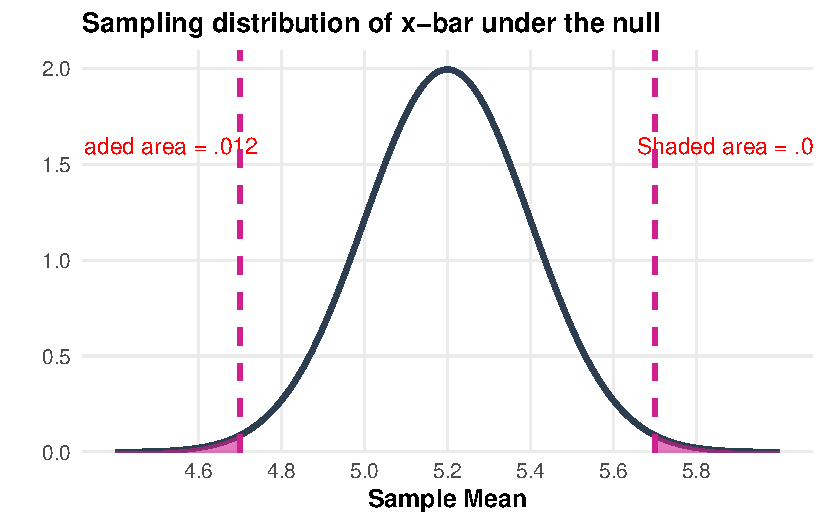
\includegraphics[keepaspectratio]{index_files/figure-pdf/unnamed-chunk-50-1.pdf}}

\begin{Shaded}
\begin{Highlighting}[]
\FunctionTok{print}\NormalTok{(p2)}
\end{Highlighting}
\end{Shaded}

\pandocbounded{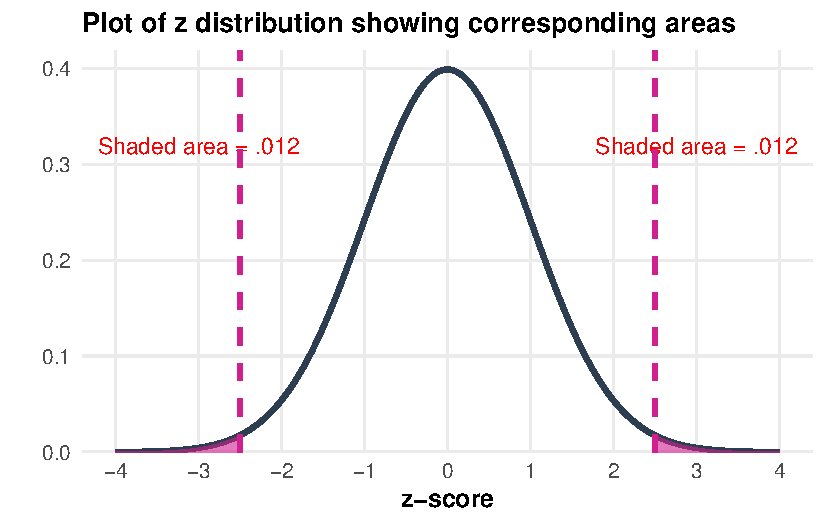
\includegraphics[keepaspectratio]{index_files/figure-pdf/unnamed-chunk-50-2.pdf}}

\subsection{Computing the Test
Statistic}\label{computing-the-test-statistic}

Find the test statistic (z-score):

\[
z = \frac{\bar{x} - \mu_0}{\sigma/\sqrt{n}} = \frac{4.7 - 5.2}{6.0/\sqrt{900}} = \frac{-0.5}{6/30} = \frac{-0.5}{0.2} = -0.5 \times 5 = -2.5
\]

\subsection{The Standardized
Distribution}\label{the-standardized-distribution}

\begin{Shaded}
\begin{Highlighting}[]
\FunctionTok{library}\NormalTok{(ggplot2)}

\CommentTok{\# Z{-}score}
\NormalTok{z\_obs }\OtherTok{\textless{}{-}} \SpecialCharTok{{-}}\FloatTok{2.5}

\CommentTok{\# Create data for standard normal}
\NormalTok{z\_vals }\OtherTok{\textless{}{-}} \FunctionTok{seq}\NormalTok{(}\SpecialCharTok{{-}}\DecValTok{4}\NormalTok{, }\DecValTok{4}\NormalTok{, }\AttributeTok{length.out =} \DecValTok{500}\NormalTok{)}
\NormalTok{z\_y }\OtherTok{\textless{}{-}} \FunctionTok{dnorm}\NormalTok{(z\_vals)}
\NormalTok{df\_z }\OtherTok{\textless{}{-}} \FunctionTok{data.frame}\NormalTok{(}\AttributeTok{z =}\NormalTok{ z\_vals, }\AttributeTok{y =}\NormalTok{ z\_y)}

\CommentTok{\# Create plot}
\FunctionTok{ggplot}\NormalTok{() }\SpecialCharTok{+}
  \CommentTok{\# Normal curve}
  \FunctionTok{geom\_line}\NormalTok{(}\AttributeTok{data =}\NormalTok{ df\_z, }\FunctionTok{aes}\NormalTok{(}\AttributeTok{x =}\NormalTok{ z, }\AttributeTok{y =}\NormalTok{ y), }
            \AttributeTok{color =} \StringTok{"\#2C3E50"}\NormalTok{, }\AttributeTok{linewidth =} \FloatTok{1.5}\NormalTok{) }\SpecialCharTok{+}
  
  \CommentTok{\# Shade the curve}
  \FunctionTok{geom\_area}\NormalTok{(}\AttributeTok{data =}\NormalTok{ df\_z, }\FunctionTok{aes}\NormalTok{(}\AttributeTok{x =}\NormalTok{ z, }\AttributeTok{y =}\NormalTok{ y),}
            \AttributeTok{fill =} \StringTok{"\#9B59B6"}\NormalTok{, }\AttributeTok{alpha =} \FloatTok{0.3}\NormalTok{) }\SpecialCharTok{+}
  
  \CommentTok{\# Mark center}
  \FunctionTok{geom\_vline}\NormalTok{(}\AttributeTok{xintercept =} \DecValTok{0}\NormalTok{, }\AttributeTok{color =} \StringTok{"\#E74C3C"}\NormalTok{, }
             \AttributeTok{linewidth =} \DecValTok{2}\NormalTok{, }\AttributeTok{linetype =} \StringTok{"solid"}\NormalTok{) }\SpecialCharTok{+}
  \FunctionTok{annotate}\NormalTok{(}\StringTok{"text"}\NormalTok{, }\AttributeTok{x =} \DecValTok{0}\NormalTok{, }\AttributeTok{y =} \FunctionTok{max}\NormalTok{(z\_y) }\SpecialCharTok{*} \FloatTok{0.5}\NormalTok{, }
           \AttributeTok{label =} \StringTok{"0"}\NormalTok{,}
           \AttributeTok{hjust =} \SpecialCharTok{{-}}\FloatTok{0.3}\NormalTok{, }\AttributeTok{size =} \DecValTok{5}\NormalTok{, }\AttributeTok{fontface =} \StringTok{"bold"}\NormalTok{, }\AttributeTok{color =} \StringTok{"\#E74C3C"}\NormalTok{) }\SpecialCharTok{+}
  
  \CommentTok{\# Mark observed z}
  \FunctionTok{geom\_vline}\NormalTok{(}\AttributeTok{xintercept =}\NormalTok{ z\_obs, }\AttributeTok{color =} \StringTok{"\#27AE60"}\NormalTok{, }
             \AttributeTok{linewidth =} \DecValTok{2}\NormalTok{, }\AttributeTok{linetype =} \StringTok{"dashed"}\NormalTok{) }\SpecialCharTok{+}
  \FunctionTok{annotate}\NormalTok{(}\StringTok{"text"}\NormalTok{, }\AttributeTok{x =}\NormalTok{ z\_obs, }\AttributeTok{y =} \FunctionTok{max}\NormalTok{(z\_y) }\SpecialCharTok{*} \FloatTok{0.7}\NormalTok{, }
           \AttributeTok{label =} \StringTok{"z = {-}2.5"}\NormalTok{,}
           \AttributeTok{hjust =} \FloatTok{1.1}\NormalTok{, }\AttributeTok{size =} \DecValTok{6}\NormalTok{, }\AttributeTok{fontface =} \StringTok{"bold"}\NormalTok{, }\AttributeTok{color =} \StringTok{"\#27AE60"}\NormalTok{) }\SpecialCharTok{+}
  
  \CommentTok{\# Axes and labels}
  \FunctionTok{scale\_x\_continuous}\NormalTok{(}\AttributeTok{breaks =} \FunctionTok{seq}\NormalTok{(}\SpecialCharTok{{-}}\DecValTok{4}\NormalTok{, }\DecValTok{4}\NormalTok{, }\AttributeTok{by =} \DecValTok{1}\NormalTok{)) }\SpecialCharTok{+}
  \FunctionTok{scale\_y\_continuous}\NormalTok{(}\AttributeTok{expand =} \FunctionTok{c}\NormalTok{(}\DecValTok{0}\NormalTok{, }\DecValTok{0}\NormalTok{), }\AttributeTok{limits =} \FunctionTok{c}\NormalTok{(}\DecValTok{0}\NormalTok{, }\FunctionTok{max}\NormalTok{(z\_y) }\SpecialCharTok{*} \FloatTok{1.1}\NormalTok{)) }\SpecialCharTok{+}
  \FunctionTok{labs}\NormalTok{(}
    \AttributeTok{title =} \StringTok{"Standard Normal Distribution (Z{-}distribution)"}\NormalTok{,}
    \AttributeTok{x =} \StringTok{"z{-}score"}\NormalTok{,}
    \AttributeTok{y =} \StringTok{"Density"}
\NormalTok{  ) }\SpecialCharTok{+}
  \FunctionTok{theme\_minimal}\NormalTok{(}\AttributeTok{base\_size =} \DecValTok{14}\NormalTok{) }\SpecialCharTok{+}
  \FunctionTok{theme}\NormalTok{(}
    \AttributeTok{plot.title =} \FunctionTok{element\_text}\NormalTok{(}\AttributeTok{face =} \StringTok{"bold"}\NormalTok{, }\AttributeTok{size =} \DecValTok{16}\NormalTok{, }\AttributeTok{hjust =} \FloatTok{0.5}\NormalTok{),}
    \AttributeTok{axis.title =} \FunctionTok{element\_text}\NormalTok{(}\AttributeTok{face =} \StringTok{"bold"}\NormalTok{, }\AttributeTok{size =} \DecValTok{13}\NormalTok{),}
    \AttributeTok{axis.text =} \FunctionTok{element\_text}\NormalTok{(}\AttributeTok{size =} \DecValTok{12}\NormalTok{),}
    \AttributeTok{panel.grid.minor =} \FunctionTok{element\_blank}\NormalTok{(),}
    \AttributeTok{panel.background =} \FunctionTok{element\_rect}\NormalTok{(}\AttributeTok{fill =} \StringTok{"white"}\NormalTok{, }\AttributeTok{color =} \ConstantTok{NA}\NormalTok{),}
    \AttributeTok{plot.background =} \FunctionTok{element\_rect}\NormalTok{(}\AttributeTok{fill =} \StringTok{"white"}\NormalTok{, }\AttributeTok{color =} \ConstantTok{NA}\NormalTok{)}
\NormalTok{  )}
\end{Highlighting}
\end{Shaded}

\begin{figure}[H]

\centering{

\pandocbounded{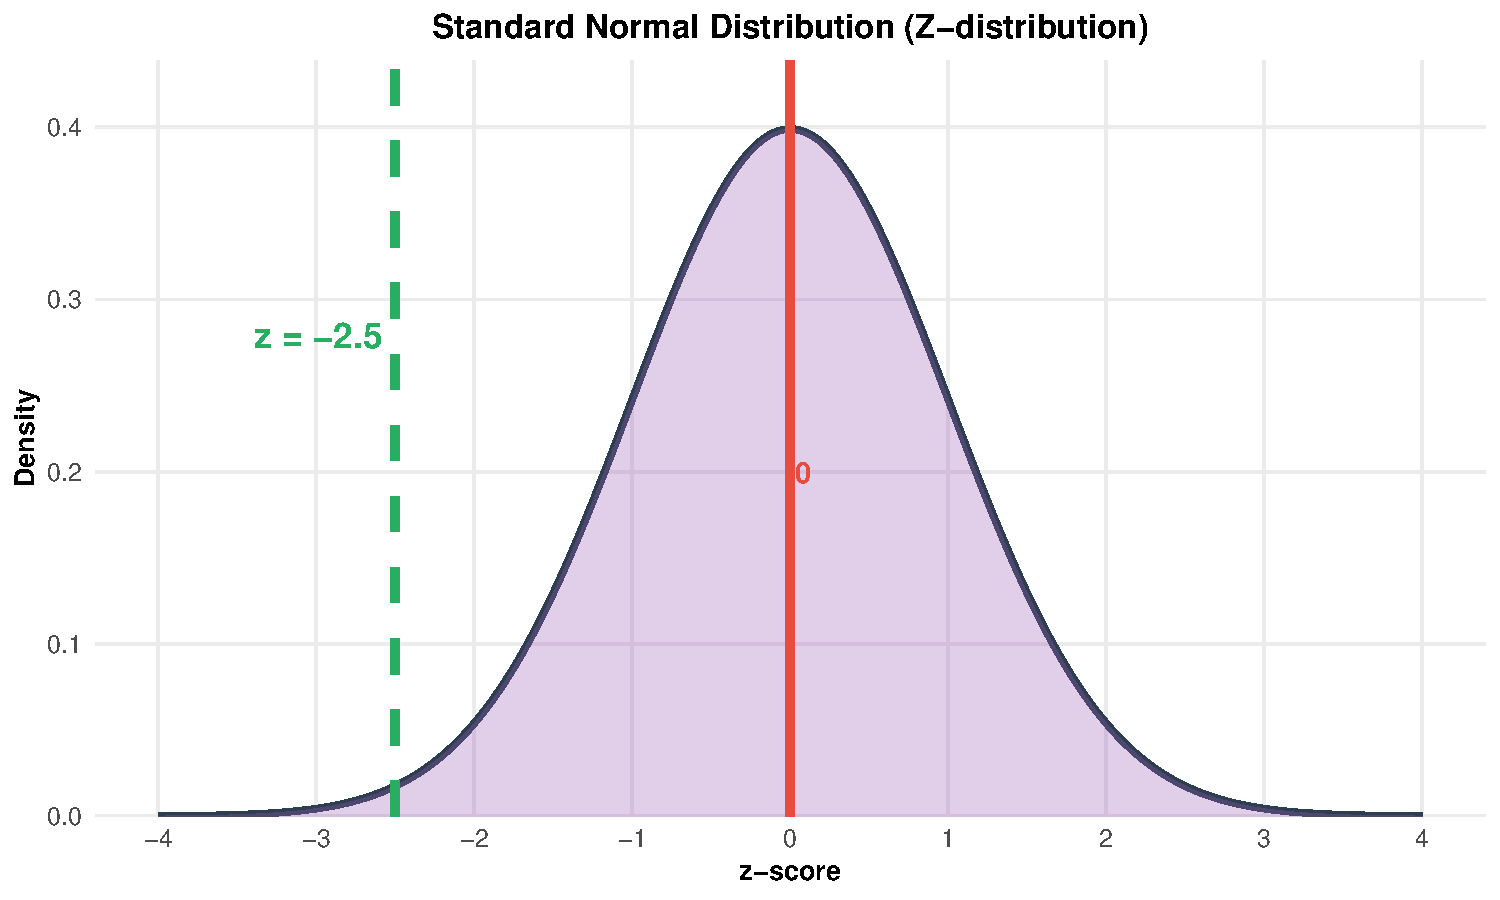
\includegraphics[keepaspectratio]{index_files/figure-pdf/fig-shakespeare-z-distribution-1.pdf}}

}

\caption{\label{fig-shakespeare-z-distribution}Standard normal
distribution showing the z-score corresponding to the observed sample
mean}

\end{figure}%

\subsection{Finding the P-value}\label{finding-the-p-value}

The P-value is the probability of obtaining results this extreme or more
extreme, assuming the null hypothesis is true:

\[
\text{P-value} = P(\bar{x} \leq 4.7 \text{ or } \bar{x} \geq 5.7)
\]

\[
= 2 \times P(Z \leq -2.5)
\]

\[
= 2 \times 0.0062 \approx 0.012
\]

\begin{Shaded}
\begin{Highlighting}[]
\FunctionTok{suppressPackageStartupMessages}\NormalTok{(\{}
  \FunctionTok{library}\NormalTok{(ggplot2)}
  \FunctionTok{library}\NormalTok{(dplyr)}
  \FunctionTok{library}\NormalTok{(tibble)}
  \FunctionTok{library}\NormalTok{(scales)}
  \FunctionTok{library}\NormalTok{(grid)     }\CommentTok{\# unit(), arrow()}
\NormalTok{\})}

\CommentTok{\# {-}{-}{-}{-}{-} Parameters {-}{-}{-}{-}{-}}
\NormalTok{mu\_0  }\OtherTok{\textless{}{-}} \FloatTok{5.2}
\NormalTok{sigma }\OtherTok{\textless{}{-}} \FloatTok{6.0}
\NormalTok{n     }\OtherTok{\textless{}{-}} \DecValTok{900}
\NormalTok{se    }\OtherTok{\textless{}{-}}\NormalTok{ sigma }\SpecialCharTok{/} \FunctionTok{sqrt}\NormalTok{(n)   }\CommentTok{\# 0.2}
\NormalTok{x\_bar }\OtherTok{\textless{}{-}} \FloatTok{4.7}
\NormalTok{x\_mir }\OtherTok{\textless{}{-}}\NormalTok{ mu\_0 }\SpecialCharTok{+}\NormalTok{ (mu\_0 }\SpecialCharTok{{-}}\NormalTok{ x\_bar)   }\CommentTok{\# mirror cutoff at 5.7}
\NormalTok{z\_obs }\OtherTok{\textless{}{-}}\NormalTok{ (x\_bar }\SpecialCharTok{{-}}\NormalTok{ mu\_0) }\SpecialCharTok{/}\NormalTok{ se     }\CommentTok{\# {-}2.5}
\NormalTok{p\_val }\OtherTok{\textless{}{-}} \DecValTok{2} \SpecialCharTok{*} \FunctionTok{pnorm}\NormalTok{(}\FunctionTok{abs}\NormalTok{(z\_obs), }\AttributeTok{lower.tail =} \ConstantTok{FALSE}\NormalTok{)}

\CommentTok{\# {-}{-}{-}{-}{-} Curves (xbar and z) {-}{-}{-}{-}{-}}
\NormalTok{x\_vals }\OtherTok{\textless{}{-}} \FunctionTok{seq}\NormalTok{(mu\_0 }\SpecialCharTok{{-}} \DecValTok{4}\SpecialCharTok{*}\NormalTok{se, mu\_0 }\SpecialCharTok{+} \DecValTok{4}\SpecialCharTok{*}\NormalTok{se, }\AttributeTok{length.out =} \DecValTok{600}\NormalTok{)}
\NormalTok{y\_vals }\OtherTok{\textless{}{-}} \FunctionTok{dnorm}\NormalTok{(x\_vals, }\AttributeTok{mean =}\NormalTok{ mu\_0, }\AttributeTok{sd =}\NormalTok{ se)}
\NormalTok{z\_vals }\OtherTok{\textless{}{-}} \FunctionTok{seq}\NormalTok{(}\SpecialCharTok{{-}}\DecValTok{4}\NormalTok{, }\DecValTok{4}\NormalTok{, }\AttributeTok{length.out =} \DecValTok{600}\NormalTok{)}
\NormalTok{z\_y    }\OtherTok{\textless{}{-}} \FunctionTok{dnorm}\NormalTok{(z\_vals)}

\NormalTok{y\_max  }\OtherTok{\textless{}{-}} \FunctionTok{max}\NormalTok{(y\_vals)  }\CommentTok{\# \textasciitilde{}1.994}
\NormalTok{z\_max  }\OtherTok{\textless{}{-}} \FunctionTok{max}\NormalTok{(z\_y)     }\CommentTok{\# \textasciitilde{}0.399}

\CommentTok{\# ASCII facet labels to avoid glyph issues}
\NormalTok{lab\_x  }\OtherTok{\textless{}{-}} \StringTok{"Sampling (xbar under H0)"}
\NormalTok{lab\_z  }\OtherTok{\textless{}{-}} \StringTok{"Z distribution"}

\CommentTok{\# Long{-}form data}
\NormalTok{df\_curve }\OtherTok{\textless{}{-}} \FunctionTok{bind\_rows}\NormalTok{(}
  \FunctionTok{tibble}\NormalTok{(}\AttributeTok{panel =}\NormalTok{ lab\_x, }\AttributeTok{x =}\NormalTok{ x\_vals, }\AttributeTok{y =}\NormalTok{ y\_vals),}
  \FunctionTok{tibble}\NormalTok{(}\AttributeTok{panel =}\NormalTok{ lab\_z, }\AttributeTok{x =}\NormalTok{ z\_vals, }\AttributeTok{y =}\NormalTok{ z\_y)}
\NormalTok{)}

\CommentTok{\# Two{-}sided shaded regions}
\NormalTok{df\_area }\OtherTok{\textless{}{-}} \FunctionTok{bind\_rows}\NormalTok{(}
  \FunctionTok{tibble}\NormalTok{(}\AttributeTok{panel =}\NormalTok{ lab\_x, }\AttributeTok{x =}\NormalTok{ x\_vals, }\AttributeTok{y =}\NormalTok{ y\_vals) }\SpecialCharTok{|\textgreater{}}
    \FunctionTok{filter}\NormalTok{(x }\SpecialCharTok{\textless{}=}\NormalTok{ x\_bar }\SpecialCharTok{|}\NormalTok{ x }\SpecialCharTok{\textgreater{}=}\NormalTok{ x\_mir),}
  \FunctionTok{tibble}\NormalTok{(}\AttributeTok{panel =}\NormalTok{ lab\_z, }\AttributeTok{x =}\NormalTok{ z\_vals, }\AttributeTok{y =}\NormalTok{ z\_y) }\SpecialCharTok{|\textgreater{}}
    \FunctionTok{filter}\NormalTok{(x }\SpecialCharTok{\textless{}=}\NormalTok{ z\_obs }\SpecialCharTok{|}\NormalTok{ x }\SpecialCharTok{\textgreater{}=} \SpecialCharTok{{-}}\NormalTok{z\_obs)}
\NormalTok{)}

\CommentTok{\# Vertical reference lines (dashed center, solid cutoffs)}
\NormalTok{df\_vline }\OtherTok{\textless{}{-}} \FunctionTok{tibble}\NormalTok{(}
  \AttributeTok{panel =} \FunctionTok{c}\NormalTok{(lab\_x, lab\_x, lab\_x,  lab\_z,  lab\_z,  lab\_z),}
  \AttributeTok{xint  =} \FunctionTok{c}\NormalTok{(mu\_0, x\_bar, x\_mir,   }\DecValTok{0}\NormalTok{,      z\_obs,  }\SpecialCharTok{{-}}\NormalTok{z\_obs),}
  \AttributeTok{type  =} \FunctionTok{c}\NormalTok{(}\StringTok{"center"}\NormalTok{,}\StringTok{"cut"}\NormalTok{,}\StringTok{"cut"}\NormalTok{, }\StringTok{"center"}\NormalTok{,}\StringTok{"cut"}\NormalTok{,}\StringTok{"cut"}\NormalTok{)}
\NormalTok{)}

\CommentTok{\# {-}{-}{-}{-}{-} Annotations (precise) {-}{-}{-}{-}{-}}
\CommentTok{\# Left panel: arrows + labels for mu0, xbar, mirror, and p}
\NormalTok{ann\_seg\_x }\OtherTok{\textless{}{-}} \FunctionTok{tribble}\NormalTok{(}
  \SpecialCharTok{\textasciitilde{}}\NormalTok{panel, }\SpecialCharTok{\textasciitilde{}}\NormalTok{x,         }\SpecialCharTok{\textasciitilde{}}\NormalTok{xend,     }\SpecialCharTok{\textasciitilde{}}\NormalTok{y,               }\SpecialCharTok{\textasciitilde{}}\NormalTok{yend,             }\SpecialCharTok{\textasciitilde{}}\NormalTok{lab,                      }\SpecialCharTok{\textasciitilde{}}\NormalTok{lx,       }\SpecialCharTok{\textasciitilde{}}\NormalTok{ly,                 }\SpecialCharTok{\textasciitilde{}}\NormalTok{hjust, }\SpecialCharTok{\textasciitilde{}}\NormalTok{vjust,}
\NormalTok{  lab\_x,  mu\_0 }\SpecialCharTok{+} \FloatTok{0.02}\NormalTok{, mu\_0,     y\_max}\SpecialCharTok{*}\FloatTok{0.92}\NormalTok{,       y\_max}\SpecialCharTok{*}\FloatTok{0.62}\NormalTok{,        }\StringTok{"mu[0]"}\NormalTok{,                  mu\_0}\FloatTok{+0.02}\NormalTok{, y\_max}\SpecialCharTok{*}\FloatTok{0.96}\NormalTok{,          }\DecValTok{0}\NormalTok{,      }\DecValTok{0}\NormalTok{,}
\NormalTok{  lab\_x,  x\_bar }\SpecialCharTok{{-}} \FloatTok{0.02}\NormalTok{, x\_bar,   y\_max}\SpecialCharTok{*}\FloatTok{0.30}\NormalTok{,       y\_max}\SpecialCharTok{*}\FloatTok{0.05}\NormalTok{,        }\StringTok{"bar(x)==4.7"}\NormalTok{,            x\_bar}\FloatTok{{-}0.02}\NormalTok{,y\_max}\SpecialCharTok{*}\FloatTok{0.34}\NormalTok{,          }\DecValTok{1}\NormalTok{,      }\DecValTok{0}\NormalTok{,}
\NormalTok{  lab\_x,  x\_mir }\SpecialCharTok{+} \FloatTok{0.02}\NormalTok{, x\_mir,   y\_max}\SpecialCharTok{*}\FloatTok{0.30}\NormalTok{,       y\_max}\SpecialCharTok{*}\FloatTok{0.05}\NormalTok{,        }\StringTok{"mu[0] + (mu[0]{-}bar(x))"}\NormalTok{, x\_mir}\FloatTok{+0.02}\NormalTok{,y\_max}\SpecialCharTok{*}\FloatTok{0.34}\NormalTok{,          }\DecValTok{0}\NormalTok{,      }\DecValTok{0}
\NormalTok{)}

\NormalTok{ann\_text\_x\_extra }\OtherTok{\textless{}{-}} \FunctionTok{tibble}\NormalTok{(}
  \AttributeTok{panel =}\NormalTok{ lab\_x,}
  \AttributeTok{x =}\NormalTok{ mu\_0, }\AttributeTok{y =}\NormalTok{ y\_max}\SpecialCharTok{*}\FloatTok{0.78}\NormalTok{,}
  \AttributeTok{lab =} \FunctionTok{paste0}\NormalTok{(}\StringTok{"p=="}\NormalTok{, }\FunctionTok{format}\NormalTok{(}\FunctionTok{round}\NormalTok{(p\_val, }\DecValTok{4}\NormalTok{), }\AttributeTok{nsmall =} \DecValTok{4}\NormalTok{))}
\NormalTok{)}

\CommentTok{\# Right panel: arrows + labels for z=0, z={-}2.5, z=+2.5, and p}
\NormalTok{ann\_seg\_z }\OtherTok{\textless{}{-}} \FunctionTok{tribble}\NormalTok{(}
  \SpecialCharTok{\textasciitilde{}}\NormalTok{panel, }\SpecialCharTok{\textasciitilde{}}\NormalTok{x,    }\SpecialCharTok{\textasciitilde{}}\NormalTok{xend,  }\SpecialCharTok{\textasciitilde{}}\NormalTok{y,            }\SpecialCharTok{\textasciitilde{}}\NormalTok{yend,         }\SpecialCharTok{\textasciitilde{}}\NormalTok{lab,          }\SpecialCharTok{\textasciitilde{}}\NormalTok{lx,   }\SpecialCharTok{\textasciitilde{}}\NormalTok{ly,            }\SpecialCharTok{\textasciitilde{}}\NormalTok{hjust, }\SpecialCharTok{\textasciitilde{}}\NormalTok{vjust,}
\NormalTok{  lab\_z,  }\FloatTok{0.10}\NormalTok{,  }\DecValTok{0}\NormalTok{,      z\_max}\SpecialCharTok{*}\FloatTok{0.92}\NormalTok{,    z\_max}\SpecialCharTok{*}\FloatTok{0.62}\NormalTok{,    }\StringTok{"z==0"}\NormalTok{,        }\FloatTok{0.10}\NormalTok{,  z\_max}\SpecialCharTok{*}\FloatTok{0.96}\NormalTok{,     }\DecValTok{0}\NormalTok{,      }\DecValTok{0}\NormalTok{,}
\NormalTok{  lab\_z, }\SpecialCharTok{{-}}\FloatTok{2.35}\NormalTok{, }\SpecialCharTok{{-}}\FloatTok{2.5}\NormalTok{,    z\_max}\SpecialCharTok{*}\FloatTok{0.38}\NormalTok{,    z\_max}\SpecialCharTok{*}\FloatTok{0.05}\NormalTok{,    }\StringTok{"z=={-}2.5"}\NormalTok{,    }\SpecialCharTok{{-}}\FloatTok{2.35}\NormalTok{,  z\_max}\SpecialCharTok{*}\FloatTok{0.42}\NormalTok{,     }\DecValTok{0}\NormalTok{,      }\DecValTok{0}\NormalTok{,}
\NormalTok{  lab\_z,  }\FloatTok{2.35}\NormalTok{,  }\FloatTok{2.5}\NormalTok{,    z\_max}\SpecialCharTok{*}\FloatTok{0.38}\NormalTok{,    z\_max}\SpecialCharTok{*}\FloatTok{0.05}\NormalTok{,    }\StringTok{"z==2.5"}\NormalTok{,      }\FloatTok{2.35}\NormalTok{,  z\_max}\SpecialCharTok{*}\FloatTok{0.42}\NormalTok{,     }\DecValTok{1}\NormalTok{,      }\DecValTok{0}
\NormalTok{)}

\NormalTok{ann\_text\_z\_extra }\OtherTok{\textless{}{-}} \FunctionTok{tibble}\NormalTok{(}
  \AttributeTok{panel =}\NormalTok{ lab\_z,}
  \AttributeTok{x =} \DecValTok{0}\NormalTok{, }\AttributeTok{y =}\NormalTok{ z\_max}\SpecialCharTok{*}\FloatTok{0.78}\NormalTok{,}
  \AttributeTok{lab =} \FunctionTok{paste0}\NormalTok{(}\StringTok{"p=="}\NormalTok{, }\FunctionTok{format}\NormalTok{(}\FunctionTok{round}\NormalTok{(p\_val, }\DecValTok{4}\NormalTok{), }\AttributeTok{nsmall =} \DecValTok{4}\NormalTok{))}
\NormalTok{)}

\CommentTok{\# {-}{-}{-}{-}{-} Plot {-}{-}{-}{-}{-}}
\FunctionTok{ggplot}\NormalTok{() }\SpecialCharTok{+}
  \CommentTok{\# Baseline at y=0}
  \FunctionTok{geom\_segment}\NormalTok{(}
    \AttributeTok{data =} \FunctionTok{tibble}\NormalTok{(}\AttributeTok{panel =} \FunctionTok{c}\NormalTok{(lab\_x, lab\_z),}
                  \AttributeTok{x =} \FunctionTok{c}\NormalTok{(}\FunctionTok{min}\NormalTok{(x\_vals), }\FunctionTok{min}\NormalTok{(z\_vals)),}
                  \AttributeTok{xend =} \FunctionTok{c}\NormalTok{(}\FunctionTok{max}\NormalTok{(x\_vals), }\FunctionTok{max}\NormalTok{(z\_vals)),}
                  \AttributeTok{y =} \DecValTok{0}\NormalTok{, }\AttributeTok{yend =} \DecValTok{0}\NormalTok{),}
    \FunctionTok{aes}\NormalTok{(}\AttributeTok{x =}\NormalTok{ x, }\AttributeTok{xend =}\NormalTok{ xend, }\AttributeTok{y =}\NormalTok{ y, }\AttributeTok{yend =}\NormalTok{ yend),}
    \AttributeTok{color =} \StringTok{"gray60"}\NormalTok{, }\AttributeTok{linewidth =} \FloatTok{0.8}
\NormalTok{  ) }\SpecialCharTok{+}
  \CommentTok{\# Red curve (thick)}
  \FunctionTok{geom\_line}\NormalTok{(}\AttributeTok{data =}\NormalTok{ df\_curve, }\FunctionTok{aes}\NormalTok{(x, y), }\AttributeTok{color =} \StringTok{"red"}\NormalTok{, }\AttributeTok{linewidth =} \FloatTok{2.4}\NormalTok{) }\SpecialCharTok{+}
  \CommentTok{\# Shaded tails (light red)}
  \FunctionTok{geom\_area}\NormalTok{(}\AttributeTok{data =}\NormalTok{ df\_area, }\FunctionTok{aes}\NormalTok{(x, y), }\AttributeTok{fill =} \StringTok{"red"}\NormalTok{, }\AttributeTok{alpha =} \FloatTok{0.25}\NormalTok{) }\SpecialCharTok{+}
  \CommentTok{\# Reference lines: dashed center, solid cutoffs}
  \FunctionTok{geom\_vline}\NormalTok{(}\AttributeTok{data =}\NormalTok{ df\_vline }\SpecialCharTok{|\textgreater{}} \FunctionTok{filter}\NormalTok{(type }\SpecialCharTok{==} \StringTok{"center"}\NormalTok{),}
             \FunctionTok{aes}\NormalTok{(}\AttributeTok{xintercept =}\NormalTok{ xint),}
             \AttributeTok{color =} \StringTok{"black"}\NormalTok{, }\AttributeTok{linewidth =} \DecValTok{1}\NormalTok{, }\AttributeTok{linetype =} \StringTok{"dashed"}\NormalTok{) }\SpecialCharTok{+}
  \FunctionTok{geom\_vline}\NormalTok{(}\AttributeTok{data =}\NormalTok{ df\_vline }\SpecialCharTok{|\textgreater{}} \FunctionTok{filter}\NormalTok{(type }\SpecialCharTok{==} \StringTok{"cut"}\NormalTok{),}
             \FunctionTok{aes}\NormalTok{(}\AttributeTok{xintercept =}\NormalTok{ xint),}
             \AttributeTok{color =} \StringTok{"black"}\NormalTok{, }\AttributeTok{linewidth =} \FloatTok{1.2}\NormalTok{, }\AttributeTok{linetype =} \StringTok{"solid"}\NormalTok{) }\SpecialCharTok{+}
  \CommentTok{\# {-}{-}{-}{-}{-} Left panel annotations {-}{-}{-}{-}{-}}
  \FunctionTok{geom\_segment}\NormalTok{(}\AttributeTok{data =}\NormalTok{ ann\_seg\_x,}
               \FunctionTok{aes}\NormalTok{(}\AttributeTok{x =}\NormalTok{ x, }\AttributeTok{xend =}\NormalTok{ xend, }\AttributeTok{y =}\NormalTok{ y, }\AttributeTok{yend =}\NormalTok{ yend),}
               \AttributeTok{arrow =} \FunctionTok{arrow}\NormalTok{(}\AttributeTok{length =} \FunctionTok{unit}\NormalTok{(}\FloatTok{0.18}\NormalTok{, }\StringTok{"cm"}\NormalTok{), }\AttributeTok{type =} \StringTok{"closed"}\NormalTok{),}
               \AttributeTok{linewidth =} \FloatTok{0.5}\NormalTok{) }\SpecialCharTok{+}
  \FunctionTok{geom\_text}\NormalTok{(}\AttributeTok{data =}\NormalTok{ ann\_seg\_x,}
            \FunctionTok{aes}\NormalTok{(}\AttributeTok{x =}\NormalTok{ lx, }\AttributeTok{y =}\NormalTok{ ly, }\AttributeTok{label =}\NormalTok{ lab, }\AttributeTok{hjust =}\NormalTok{ hjust, }\AttributeTok{vjust =}\NormalTok{ vjust),}
            \AttributeTok{parse =} \ConstantTok{TRUE}\NormalTok{, }\AttributeTok{size =} \FloatTok{4.8}\NormalTok{) }\SpecialCharTok{+}
  \FunctionTok{geom\_text}\NormalTok{(}\AttributeTok{data =}\NormalTok{ ann\_text\_x\_extra,}
            \FunctionTok{aes}\NormalTok{(}\AttributeTok{x =}\NormalTok{ x, }\AttributeTok{y =}\NormalTok{ y, }\AttributeTok{label =}\NormalTok{ lab),}
            \AttributeTok{parse =} \ConstantTok{TRUE}\NormalTok{, }\AttributeTok{fontface =} \StringTok{"bold"}\NormalTok{, }\AttributeTok{size =} \FloatTok{4.8}\NormalTok{) }\SpecialCharTok{+}
  \CommentTok{\# {-}{-}{-}{-}{-} Right panel annotations {-}{-}{-}{-}{-}}
  \FunctionTok{geom\_segment}\NormalTok{(}\AttributeTok{data =}\NormalTok{ ann\_seg\_z,}
               \FunctionTok{aes}\NormalTok{(}\AttributeTok{x =}\NormalTok{ x, }\AttributeTok{xend =}\NormalTok{ xend, }\AttributeTok{y =}\NormalTok{ y, }\AttributeTok{yend =}\NormalTok{ yend),}
               \AttributeTok{arrow =} \FunctionTok{arrow}\NormalTok{(}\AttributeTok{length =} \FunctionTok{unit}\NormalTok{(}\FloatTok{0.18}\NormalTok{, }\StringTok{"cm"}\NormalTok{), }\AttributeTok{type =} \StringTok{"closed"}\NormalTok{),}
               \AttributeTok{linewidth =} \FloatTok{0.5}\NormalTok{) }\SpecialCharTok{+}
  \FunctionTok{geom\_text}\NormalTok{(}\AttributeTok{data =}\NormalTok{ ann\_seg\_z,}
            \FunctionTok{aes}\NormalTok{(}\AttributeTok{x =}\NormalTok{ lx, }\AttributeTok{y =}\NormalTok{ ly, }\AttributeTok{label =}\NormalTok{ lab, }\AttributeTok{hjust =}\NormalTok{ hjust, }\AttributeTok{vjust =}\NormalTok{ vjust),}
            \AttributeTok{parse =} \ConstantTok{TRUE}\NormalTok{, }\AttributeTok{size =} \FloatTok{4.8}\NormalTok{) }\SpecialCharTok{+}
  \FunctionTok{geom\_text}\NormalTok{(}\AttributeTok{data =}\NormalTok{ ann\_text\_z\_extra,}
            \FunctionTok{aes}\NormalTok{(}\AttributeTok{x =}\NormalTok{ x, }\AttributeTok{y =}\NormalTok{ y, }\AttributeTok{label =}\NormalTok{ lab),}
            \AttributeTok{parse =} \ConstantTok{TRUE}\NormalTok{, }\AttributeTok{fontface =} \StringTok{"bold"}\NormalTok{, }\AttributeTok{size =} \FloatTok{4.8}\NormalTok{) }\SpecialCharTok{+}
  \FunctionTok{facet\_wrap}\NormalTok{(}\SpecialCharTok{\textasciitilde{}}\NormalTok{ panel, }\AttributeTok{scales =} \StringTok{"free"}\NormalTok{, }\AttributeTok{ncol =} \DecValTok{2}\NormalTok{) }\SpecialCharTok{+}
  \CommentTok{\# Plotmath title/subtitle (robust across fonts)}
  \FunctionTok{labs}\NormalTok{(}
    \AttributeTok{title =} \FunctionTok{expression}\NormalTok{(}\StringTok{"Two{-}sided "} \SpecialCharTok{*}\NormalTok{ p }\SpecialCharTok{*} \StringTok{"{-}value under "} \SpecialCharTok{*}\NormalTok{ H[}\DecValTok{0}\NormalTok{]),}
    \AttributeTok{subtitle =} \FunctionTok{bquote}\NormalTok{(}\FunctionTok{bar}\NormalTok{(x) }\SpecialCharTok{==}\NormalTok{ .(x\_bar) }\SpecialCharTok{*} \StringTok{", "} \SpecialCharTok{\textasciitilde{}}
\NormalTok{                      mu[}\DecValTok{0}\NormalTok{] }\SpecialCharTok{==}\NormalTok{ .(mu\_0) }\SpecialCharTok{*} \StringTok{", "} \SpecialCharTok{\textasciitilde{}}
\NormalTok{                      SE }\SpecialCharTok{==}\NormalTok{ .(}\FunctionTok{round}\NormalTok{(se, }\DecValTok{1}\NormalTok{)) }\SpecialCharTok{*} \StringTok{", "} \SpecialCharTok{\textasciitilde{}}
\NormalTok{                      z }\SpecialCharTok{==}\NormalTok{ .(}\FunctionTok{round}\NormalTok{(z\_obs, }\DecValTok{1}\NormalTok{)) }\SpecialCharTok{\textasciitilde{}} \StringTok{"  "} \SpecialCharTok{*} \StringTok{"{-}\textgreater{}"} \SpecialCharTok{*} \StringTok{"  "} \SpecialCharTok{\textasciitilde{}}
\NormalTok{                      p }\SpecialCharTok{==}\NormalTok{ .(}\FunctionTok{round}\NormalTok{(p\_val, }\DecValTok{4}\NormalTok{))),}
    \AttributeTok{x =} \ConstantTok{NULL}\NormalTok{, }\AttributeTok{y =} \ConstantTok{NULL}
\NormalTok{  ) }\SpecialCharTok{+}
  \FunctionTok{scale\_y\_continuous}\NormalTok{(}\AttributeTok{limits =} \FunctionTok{c}\NormalTok{(}\DecValTok{0}\NormalTok{, }\ConstantTok{NA}\NormalTok{), }\AttributeTok{expand =} \FunctionTok{expansion}\NormalTok{(}\AttributeTok{mult =} \FunctionTok{c}\NormalTok{(}\DecValTok{0}\NormalTok{, }\FloatTok{0.05}\NormalTok{))) }\SpecialCharTok{+}
  \FunctionTok{theme\_minimal}\NormalTok{(}\AttributeTok{base\_size =} \DecValTok{16}\NormalTok{) }\SpecialCharTok{+}
  \FunctionTok{theme}\NormalTok{(}
    \AttributeTok{plot.title   =} \FunctionTok{element\_text}\NormalTok{(}\AttributeTok{face =} \StringTok{"bold"}\NormalTok{),}
    \AttributeTok{strip.text   =} \FunctionTok{element\_text}\NormalTok{(}\AttributeTok{face =} \StringTok{"bold"}\NormalTok{),}
    \AttributeTok{panel.grid   =} \FunctionTok{element\_blank}\NormalTok{(),}
    \AttributeTok{panel.background =} \FunctionTok{element\_rect}\NormalTok{(}\AttributeTok{fill =} \StringTok{"white"}\NormalTok{, }\AttributeTok{color =} \ConstantTok{NA}\NormalTok{),}
    \AttributeTok{plot.background  =} \FunctionTok{element\_rect}\NormalTok{(}\AttributeTok{fill =} \StringTok{"white"}\NormalTok{, }\AttributeTok{color =} \ConstantTok{NA}\NormalTok{),}
    \AttributeTok{panel.spacing    =} \FunctionTok{unit}\NormalTok{(}\DecValTok{16}\NormalTok{, }\StringTok{"pt"}\NormalTok{)}
\NormalTok{  )}
\end{Highlighting}
\end{Shaded}

\begin{figure}[H]

\centering{

\pandocbounded{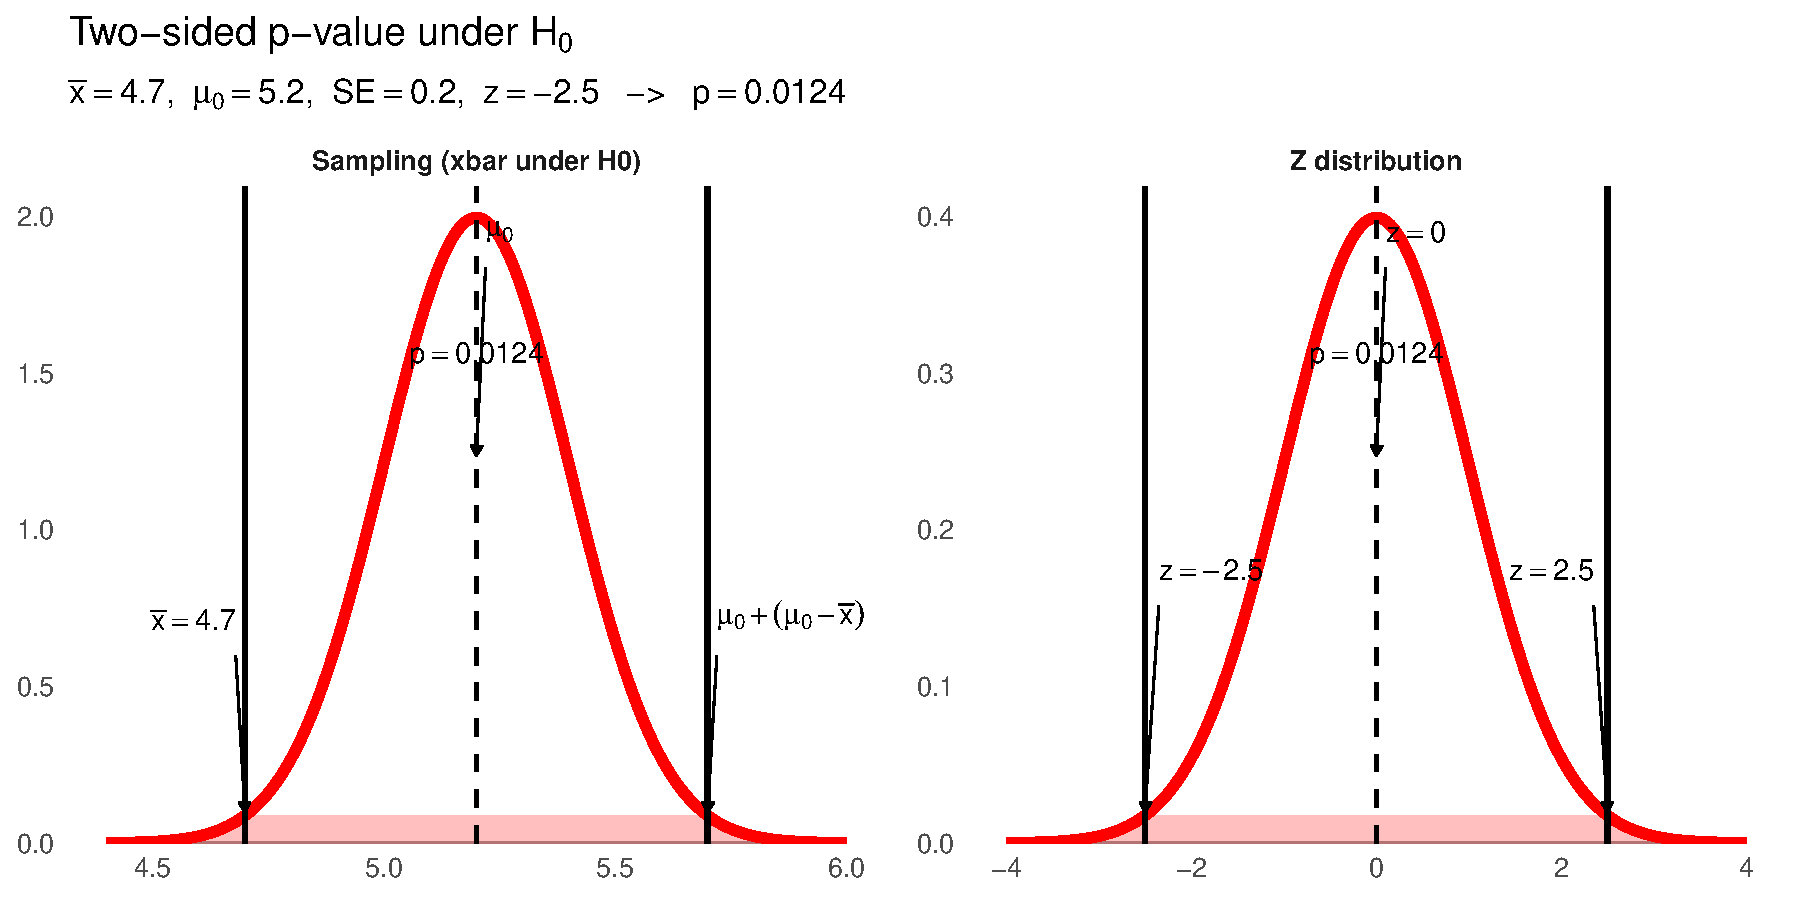
\includegraphics[keepaspectratio]{index_files/figure-pdf/fig-shakespeare-pvalue-facet-pnas-annotated-1.pdf}}

}

\caption{\label{fig-shakespeare-pvalue-facet-pnas-annotated}Left:
sampling distribution of \(\bar{x}\) under \(H_0\) with two-sided
\(p\)-value regions shaded and annotated. Right: corresponding standard
normal (\(z\)) picture with the same two-sided regions.}

\end{figure}%

\subsection{Interpreting the P-value}\label{interpreting-the-p-value}

\textbf{Question:} Is this good evidence against the null hypothesis?

\textbf{Answer:} Yes! With a P-value of 0.012, we have strong evidence
against the null hypothesis. This means that if Shakespeare truly wrote
the scene, there is only a 1.2\% chance we would observe a sample mean
word length as extreme as 4.7 (or more extreme).

At the conventional significance level of \(\alpha = 0.05\), we would
\textbf{reject the null hypothesis} because \(0.012 < 0.05\). This
provides evidence that Shakespeare likely did not write this scene.

\subsection{Alternative Scenarios}\label{alternative-scenarios}

\textbf{Scenario 1:} Suppose the average word length had been 5.0
instead of 4.7.

Would this be convincing evidence against the null hypothesis?

\emph{(Do we need the exact P-value to decide this? How about just
looking at our x-scale sketch?)}

The z-score would be: \[
z = \frac{5.0 - 5.2}{0.2} = \frac{-0.2}{0.2} = -1.0
\]

This is much closer to the hypothesized mean. Looking at the sampling
distribution, a value of 5.0 falls well within the typical range of
variation we would expect if \(\mu = 5.2\). The P-value would be much
larger (approximately 0.32), so we would \textbf{not reject} the null
hypothesis.

\textbf{Scenario 2:} What if the average word length had been 10.0?

This would yield: \[
z = \frac{10.0 - 5.2}{0.2} = \frac{4.8}{0.2} = 24
\]

This is extraordinarily far from the hypothesized mean---so extreme that
the P-value would be essentially zero. We would have
\textbf{overwhelming evidence} to reject the null hypothesis. A mean
word length of 10.0 would be completely inconsistent with Shakespeare's
known writing style.

\subsection{Interpreting P-values}\label{interpreting-p-values}

Here is the basic P-value issue: Could random variation alone, because
of the sampling process, account for the difference between the null
value and a value obtained from a random sample?

\subsection{Small P-values:}\label{small-p-values}

\begin{itemize}
\item
  Imply that random variation alone is not likely to account for the
  observed difference
\item
  Give evidence against \(H_0\), suggesting that the true property of
  the population is significantly different from what was stated in
  \(H_0\)
\end{itemize}

\subsection{How small is small enough?}\label{how-small-is-small-enough}

Standard significance levels, represented by \(\alpha\) (alpha), provide
\emph{decision rules}:

\begin{itemize}
\tightlist
\item
  \(\alpha = 0.05\): ``Significant at the 5\% level''
\item
  \(\alpha = 0.01\): ``Significant at the 1\% level''
\end{itemize}

\textbf{Decision rule:} If the P-value is smaller than one of these
\(\alpha\) values, we reject \(H_0\) and make the indicated conclusion
at that \emph{level of significance}.

\subsection{\texorpdfstring{The Significance Level, \(\alpha\): A
Standard of
Evidence}{The Significance Level, \textbackslash alpha: A Standard of Evidence}}\label{the-significance-level-alpha-a-standard-of-evidence}

The significance level, \(\alpha\), is the largest P-value tolerated for
rejecting the null hypothesis. It indicates how much evidence against
\(H_0\) will be required to reject it. This value is decided upon
\emph{before} conducting the test.

\textbf{Decision rules:}

\begin{itemize}
\item
  If the P-value is equal to or less than \(\alpha\), then we reject
  \(H_0\)
\item
  If the P-value is greater than \(\alpha\), then we fail to reject
  \(H_0\)
\end{itemize}

The choice of \(\alpha\) represents a balance between two types of
errors (which we will explore in the next section) and reflects the
consequences of making a wrong decision in the specific research
context.

\subsection{\texorpdfstring{Example Using Two Common Values of
\(\alpha\): .05 and
.01}{Example Using Two Common Values of \textbackslash alpha: .05 and .01}}\label{example-using-two-common-values-of-alpha-.05-and-.01}

Suppose our P-value is .03 for some obtained results.

In other words, the probability of getting a sample mean as extreme or
more extreme as ours just by chance if the null were true is .03.

If \(\alpha\) had been set ahead of time to 5\% (\(\alpha = .05\)), then
the obtained P-value would be regarded as \emph{statistically
significant}.

If \(\alpha\) had been set to 1\% (\(\alpha = .01\)), then the obtained
P-value would not be regarded as significant.

In this case, we say that ``our results are significant at the .05 or
5\% level but not at the .01 or 1\% level.''

Formally, and ideally, we decide ahead of time what \(\alpha\) level we
are using, and therefore what P-values will be considered significant
evidence against our null hypothesis.

Many researchers today advocate the use of \emph{much} smaller values of
\(\alpha\).

\#\#\#Fixed \(\alpha\)-Level Example

Typically a researcher explicitly determines a fixed \(\alpha\)-level
before examining the data.

In the Shakespeare example, the test might be set up as two-sided, with
fixed alpha-level, \(\alpha = .05\).

Then the obtained P-value, for \(z = -2.5\), namely, \(p = 0.012\), is
interpreted as evidence sufficient to reject \(H_0\) without any
ambiguity.

(An older method of doing a fixed \(\alpha\)-level test involved
calculating \emph{critical values} of \(z\) that would lead to
rejection. E.g., \(z^* = \pm 1.96\). That method avoided calculating the
P-value because it was time-consuming. Today computers routinely provide
P-values, making this method obsolete.)

\section{How Can We Justify One-Sided
Tests?}\label{how-can-we-justify-one-sided-tests}

It can be tempting to use a one-sided test because the P-value won't
have to be doubled to take into account the other tail. This increases
the opportunity for claiming a significant result.But we should always
have a serious reason for stating that we are interested in only a
single tail. This should be based on theory if possible.We should think
about what we would do if the result came out in the other tail.One
thing we could not do in such a case is claim a ``significant result,''
since our hypothesis did not involve that tail. Many social science
studies are so weakly grounded in theory that results in either tail
would be informative. In such cases, two-sided tests should be used.

\section{Always Avoid Saying the Null ``Is
Accepted''}\label{always-avoid-saying-the-null-is-accepted}

We should \emph{always} say we \emph{fail to reject} \(H_0\) rather than
we \emph{accept} \(H_0\) when the P-value does not meet our chosen
significance level (i.e., \(p > \alpha\)).

It is pretty clear we should avoid saying we ``accept \(H_0\)'' in
two-sided tests, since \(H_0\) is actually asserting that the parameter
equals a particular, point value. (For example, \(H_0: \mu = 5.2\).)

Although we may be comfortable saying our evidence does not argue
\emph{against} the statement that the point value is correct, this is
different from saying that it argues \emph{for} that the point value is
correct.

But another possibility is more subtle: If we fail to reject in a
one-sided test, say \(H_0: \mu > \mu_0\), this \emph{does not} mean that
\(\mu\) is less than \(\mu_0\). It might well be somewhat larger than
\(\mu_0\) (making the null false), but not so large that it produced an
\(\bar{x}\) value leading to rejection of the null in the test.

\section{\texorpdfstring{Correctly Place \(\mu_0\) in the Null
Hypothesis}{Correctly Place \textbackslash mu\_0 in the Null Hypothesis}}\label{correctly-place-mu_0-in-the-null-hypothesis}

Suppose a researcher claims that the mean number of ``SMS language''
terms (lol, omg, etc.) UW students can identify is \emph{at least} 20.

What is an appropriate choice for the alternative hypothesis?

The alternative hypothesis (\(H_a\)) should be the thing the researcher
is trying to establish evidence for.

This suggests that the alternative should be \(H_a: \mu \geq 20\), since
the researcher included 20 in the statement ``\emph{at least} 20.''

But that would be a mistake.

The null \emph{must} contain the null value \(\mu_0 = 20\), since we
need to find evidence against the null by calculating a sampling
distribution at a particular value, and putting \(\mu_0\) into the null
gives us such a value.

You should put the \(\mu_0\) value into the null hypothesis regardless
of how an original question might be verbally worded.

In this case the correct hypotheses are: \(H_0: \mu = 20\);
\(H_a: \mu > 20\)

\section{Hypothesis Test Conclusions from Confidence
Intervals}\label{hypothesis-test-conclusions-from-confidence-intervals}

Since a confidence interval and a two-sided hypothesis test both involve
the same standard error, \(\sigma/\sqrt{n}\), observing whether
\(\mu_0\) lies outside a confidence interval is equivalent to a
two-sided test of \(H_0: \mu = \mu_0\).

This equivalence occurs for a two-sided test at level \(\alpha\) and a
\(C = 1 - \alpha\) confidence interval.

In the Shakespeare example, the z statistic for the test was
\(z = 2.5\), leading to rejection of \(H_0: \mu = 5.2\), using
\(\alpha = .05\), two-tailed.

It is then also necessarily true that a 95\% CI around the sample mean,
\(4.7 \pm 1.96(6/30) = [4.31, 5.09]\) does not include 5.2.

The next slide diagrams the situation.

\section{Tests from Confidence Intervals
(2)}\label{tests-from-confidence-intervals-2}

To reject \(H_0: \mu = \mu_0\), two-sided, at \(\alpha = 0.05\),
\(\bar{x}\) would have to differ from \(\mu_0\) by at least
\(z^*(\sigma/\sqrt{n})\) in either direction:

\begin{Shaded}
\begin{Highlighting}[]
\FunctionTok{library}\NormalTok{(ggplot2)}

\CommentTok{\# Parameters}
\NormalTok{mu\_0 }\OtherTok{\textless{}{-}} \FloatTok{5.2}
\NormalTok{x\_bar }\OtherTok{\textless{}{-}} \FloatTok{4.7}
\NormalTok{sigma }\OtherTok{\textless{}{-}} \FloatTok{6.0}
\NormalTok{n }\OtherTok{\textless{}{-}} \DecValTok{900}
\NormalTok{se }\OtherTok{\textless{}{-}}\NormalTok{ sigma }\SpecialCharTok{/} \FunctionTok{sqrt}\NormalTok{(n)}
\NormalTok{z\_star }\OtherTok{\textless{}{-}} \FloatTok{1.96}
\NormalTok{margin }\OtherTok{\textless{}{-}}\NormalTok{ z\_star }\SpecialCharTok{*}\NormalTok{ se}

\CommentTok{\# Create normal distribution data}
\NormalTok{x\_vals }\OtherTok{\textless{}{-}} \FunctionTok{seq}\NormalTok{(mu\_0 }\SpecialCharTok{{-}} \DecValTok{4}\SpecialCharTok{*}\NormalTok{se, mu\_0 }\SpecialCharTok{+} \DecValTok{4}\SpecialCharTok{*}\NormalTok{se, }\AttributeTok{length.out =} \DecValTok{500}\NormalTok{)}
\NormalTok{y\_vals }\OtherTok{\textless{}{-}} \FunctionTok{dnorm}\NormalTok{(x\_vals, }\AttributeTok{mean =}\NormalTok{ mu\_0, }\AttributeTok{sd =}\NormalTok{ se)}
\NormalTok{df\_curve }\OtherTok{\textless{}{-}} \FunctionTok{data.frame}\NormalTok{(}\AttributeTok{x =}\NormalTok{ x\_vals, }\AttributeTok{y =}\NormalTok{ y\_vals)}

\CommentTok{\# Y position for annotations}
\NormalTok{y\_max }\OtherTok{\textless{}{-}} \FunctionTok{max}\NormalTok{(y\_vals)}

\FunctionTok{ggplot}\NormalTok{() }\SpecialCharTok{+}
  \CommentTok{\# Normal curve}
  \FunctionTok{geom\_line}\NormalTok{(}\AttributeTok{data =}\NormalTok{ df\_curve, }\FunctionTok{aes}\NormalTok{(}\AttributeTok{x =}\NormalTok{ x, }\AttributeTok{y =}\NormalTok{ y), }
            \AttributeTok{color =} \StringTok{"red"}\NormalTok{, }\AttributeTok{linewidth =} \DecValTok{3}\NormalTok{) }\SpecialCharTok{+}
  
  \CommentTok{\# Horizontal line at base of curve}
  \FunctionTok{geom\_segment}\NormalTok{(}\FunctionTok{aes}\NormalTok{(}\AttributeTok{x =} \FunctionTok{min}\NormalTok{(x\_vals), }\AttributeTok{xend =} \FunctionTok{max}\NormalTok{(x\_vals), }
                   \AttributeTok{y =} \DecValTok{0}\NormalTok{, }\AttributeTok{yend =} \DecValTok{0}\NormalTok{),}
               \AttributeTok{color =} \StringTok{"gray60"}\NormalTok{, }\AttributeTok{linewidth =} \DecValTok{1}\NormalTok{) }\SpecialCharTok{+}
  
  \CommentTok{\# Vertical line at mu\_0 (dashed)}
  \FunctionTok{geom\_segment}\NormalTok{(}\FunctionTok{aes}\NormalTok{(}\AttributeTok{x =}\NormalTok{ mu\_0, }\AttributeTok{xend =}\NormalTok{ mu\_0, }\AttributeTok{y =} \DecValTok{0}\NormalTok{, }\AttributeTok{yend =}\NormalTok{ y\_max }\SpecialCharTok{*} \FloatTok{0.5}\NormalTok{),}
               \AttributeTok{color =} \StringTok{"black"}\NormalTok{, }\AttributeTok{linewidth =} \DecValTok{1}\NormalTok{, }\AttributeTok{linetype =} \StringTok{"dashed"}\NormalTok{) }\SpecialCharTok{+}
  
  \CommentTok{\# Vertical lines at rejection boundaries (solid, black)}
  \FunctionTok{geom\_segment}\NormalTok{(}\FunctionTok{aes}\NormalTok{(}\AttributeTok{x =}\NormalTok{ mu\_0 }\SpecialCharTok{{-}}\NormalTok{ margin, }\AttributeTok{xend =}\NormalTok{ mu\_0 }\SpecialCharTok{{-}}\NormalTok{ margin, }
                   \AttributeTok{y =} \DecValTok{0}\NormalTok{, }\AttributeTok{yend =}\NormalTok{ y\_max }\SpecialCharTok{*} \FloatTok{0.5}\NormalTok{),}
               \AttributeTok{color =} \StringTok{"black"}\NormalTok{, }\AttributeTok{linewidth =} \FloatTok{1.2}\NormalTok{, }\AttributeTok{linetype =} \StringTok{"solid"}\NormalTok{) }\SpecialCharTok{+}
  \FunctionTok{geom\_segment}\NormalTok{(}\FunctionTok{aes}\NormalTok{(}\AttributeTok{x =}\NormalTok{ mu\_0 }\SpecialCharTok{+}\NormalTok{ margin, }\AttributeTok{xend =}\NormalTok{ mu\_0 }\SpecialCharTok{+}\NormalTok{ margin, }
                   \AttributeTok{y =} \DecValTok{0}\NormalTok{, }\AttributeTok{yend =}\NormalTok{ y\_max }\SpecialCharTok{*} \FloatTok{0.5}\NormalTok{),}
               \AttributeTok{color =} \StringTok{"black"}\NormalTok{, }\AttributeTok{linewidth =} \FloatTok{1.2}\NormalTok{, }\AttributeTok{linetype =} \StringTok{"solid"}\NormalTok{) }\SpecialCharTok{+}
  
  \CommentTok{\# Dashed vertical lines from CI endpoints to distribution}
  \FunctionTok{geom\_segment}\NormalTok{(}\FunctionTok{aes}\NormalTok{(}\AttributeTok{x =}\NormalTok{ x\_bar }\SpecialCharTok{{-}}\NormalTok{ margin, }\AttributeTok{xend =}\NormalTok{ x\_bar }\SpecialCharTok{{-}}\NormalTok{ margin,}
                   \AttributeTok{y =} \SpecialCharTok{{-}}\NormalTok{y\_max }\SpecialCharTok{*} \FloatTok{0.35}\NormalTok{, }\AttributeTok{yend =} \DecValTok{0}\NormalTok{),}
               \AttributeTok{color =} \StringTok{"black"}\NormalTok{, }\AttributeTok{linewidth =} \FloatTok{0.8}\NormalTok{, }\AttributeTok{linetype =} \StringTok{"dashed"}\NormalTok{) }\SpecialCharTok{+}
  \FunctionTok{geom\_segment}\NormalTok{(}\FunctionTok{aes}\NormalTok{(}\AttributeTok{x =}\NormalTok{ x\_bar, }\AttributeTok{xend =}\NormalTok{ x\_bar,}
                   \AttributeTok{y =} \SpecialCharTok{{-}}\NormalTok{y\_max }\SpecialCharTok{*} \FloatTok{0.35}\NormalTok{, }\AttributeTok{yend =} \DecValTok{0}\NormalTok{),}
               \AttributeTok{color =} \StringTok{"black"}\NormalTok{, }\AttributeTok{linewidth =} \FloatTok{0.8}\NormalTok{, }\AttributeTok{linetype =} \StringTok{"dashed"}\NormalTok{) }\SpecialCharTok{+}
  
  \CommentTok{\# Label for mu\_0 with arrow}
  \FunctionTok{annotate}\NormalTok{(}\StringTok{"segment"}\NormalTok{, }\AttributeTok{x =}\NormalTok{ mu\_0 }\SpecialCharTok{+} \FloatTok{0.05}\NormalTok{, }\AttributeTok{xend =}\NormalTok{ mu\_0, }
           \AttributeTok{y =}\NormalTok{ y\_max }\SpecialCharTok{*} \FloatTok{0.85}\NormalTok{, }\AttributeTok{yend =}\NormalTok{ y\_max }\SpecialCharTok{*} \FloatTok{0.55}\NormalTok{,}
           \AttributeTok{arrow =} \FunctionTok{arrow}\NormalTok{(}\AttributeTok{length =} \FunctionTok{unit}\NormalTok{(}\FloatTok{0.2}\NormalTok{, }\StringTok{"cm"}\NormalTok{), }\AttributeTok{type =} \StringTok{"closed"}\NormalTok{),}
           \AttributeTok{linewidth =} \FloatTok{0.5}\NormalTok{) }\SpecialCharTok{+}
  \FunctionTok{annotate}\NormalTok{(}\StringTok{"text"}\NormalTok{, }\AttributeTok{x =}\NormalTok{ mu\_0 }\SpecialCharTok{+} \FloatTok{0.05}\NormalTok{, }\AttributeTok{y =}\NormalTok{ y\_max }\SpecialCharTok{*} \FloatTok{0.95}\NormalTok{, }
           \AttributeTok{label =} \StringTok{"mu[0] == 5.2"}\NormalTok{,}
           \AttributeTok{size =} \DecValTok{9}\NormalTok{, }\AttributeTok{hjust =} \DecValTok{0}\NormalTok{, }\AttributeTok{color =} \StringTok{"black"}\NormalTok{, }\AttributeTok{parse =} \ConstantTok{TRUE}\NormalTok{) }\SpecialCharTok{+}
  
  \CommentTok{\# Labels for rejection boundaries with arrows}
  \FunctionTok{annotate}\NormalTok{(}\StringTok{"segment"}\NormalTok{, }\AttributeTok{x =}\NormalTok{ mu\_0 }\SpecialCharTok{{-}}\NormalTok{ margin }\SpecialCharTok{{-}} \FloatTok{0.05}\NormalTok{, }\AttributeTok{xend =}\NormalTok{ mu\_0 }\SpecialCharTok{{-}}\NormalTok{ margin, }
           \AttributeTok{y =}\NormalTok{ y\_max }\SpecialCharTok{*} \FloatTok{1.0}\NormalTok{, }\AttributeTok{yend =}\NormalTok{ y\_max }\SpecialCharTok{*} \FloatTok{0.7}\NormalTok{,}
           \AttributeTok{arrow =} \FunctionTok{arrow}\NormalTok{(}\AttributeTok{length =} \FunctionTok{unit}\NormalTok{(}\FloatTok{0.2}\NormalTok{, }\StringTok{"cm"}\NormalTok{), }\AttributeTok{type =} \StringTok{"closed"}\NormalTok{),}
           \AttributeTok{linewidth =} \FloatTok{0.5}\NormalTok{) }\SpecialCharTok{+}
  \FunctionTok{annotate}\NormalTok{(}\StringTok{"text"}\NormalTok{, }\AttributeTok{x =}\NormalTok{ mu\_0 }\SpecialCharTok{{-}}\NormalTok{ margin }\SpecialCharTok{{-}} \FloatTok{0.05}\NormalTok{, }\AttributeTok{y =}\NormalTok{ y\_max }\SpecialCharTok{*} \FloatTok{1.1}\NormalTok{, }
           \AttributeTok{label =} \StringTok{"mu[0] {-} z\^{}\textquotesingle{}*\textquotesingle{}*(sigma/sqrt(n))"}\NormalTok{,}
           \AttributeTok{size =} \DecValTok{9}\NormalTok{, }\AttributeTok{hjust =} \DecValTok{1}\NormalTok{, }\AttributeTok{color =} \StringTok{"black"}\NormalTok{, }\AttributeTok{parse =} \ConstantTok{TRUE}\NormalTok{) }\SpecialCharTok{+}
  
  \FunctionTok{annotate}\NormalTok{(}\StringTok{"segment"}\NormalTok{, }\AttributeTok{x =}\NormalTok{ mu\_0 }\SpecialCharTok{+}\NormalTok{ margin }\SpecialCharTok{+} \FloatTok{0.05}\NormalTok{, }\AttributeTok{xend =}\NormalTok{ mu\_0 }\SpecialCharTok{+}\NormalTok{ margin, }
           \AttributeTok{y =}\NormalTok{ y\_max }\SpecialCharTok{*} \FloatTok{1.0}\NormalTok{, }\AttributeTok{yend =}\NormalTok{ y\_max }\SpecialCharTok{*} \FloatTok{0.7}\NormalTok{,}
           \AttributeTok{arrow =} \FunctionTok{arrow}\NormalTok{(}\AttributeTok{length =} \FunctionTok{unit}\NormalTok{(}\FloatTok{0.2}\NormalTok{, }\StringTok{"cm"}\NormalTok{), }\AttributeTok{type =} \StringTok{"closed"}\NormalTok{),}
           \AttributeTok{linewidth =} \FloatTok{0.5}\NormalTok{) }\SpecialCharTok{+}
  \FunctionTok{annotate}\NormalTok{(}\StringTok{"text"}\NormalTok{, }\AttributeTok{x =}\NormalTok{ mu\_0 }\SpecialCharTok{+}\NormalTok{ margin }\SpecialCharTok{+} \FloatTok{0.05}\NormalTok{, }\AttributeTok{y =}\NormalTok{ y\_max }\SpecialCharTok{*} \FloatTok{1.1}\NormalTok{, }
           \AttributeTok{label =} \StringTok{"mu[0] + z\^{}\textquotesingle{}*\textquotesingle{}*(sigma/sqrt(n))"}\NormalTok{,}
           \AttributeTok{size =} \DecValTok{9}\NormalTok{, }\AttributeTok{hjust =} \DecValTok{0}\NormalTok{, }\AttributeTok{color =} \StringTok{"black"}\NormalTok{, }\AttributeTok{parse =} \ConstantTok{TRUE}\NormalTok{) }\SpecialCharTok{+}
  
  \CommentTok{\# Confidence interval horizontal line}
  \FunctionTok{geom\_segment}\NormalTok{(}\FunctionTok{aes}\NormalTok{(}\AttributeTok{x =}\NormalTok{ x\_bar }\SpecialCharTok{{-}}\NormalTok{ margin, }\AttributeTok{xend =}\NormalTok{ x\_bar }\SpecialCharTok{+}\NormalTok{ margin, }
                   \AttributeTok{y =} \SpecialCharTok{{-}}\NormalTok{y\_max }\SpecialCharTok{*} \FloatTok{0.35}\NormalTok{, }\AttributeTok{yend =} \SpecialCharTok{{-}}\NormalTok{y\_max }\SpecialCharTok{*} \FloatTok{0.35}\NormalTok{),}
               \AttributeTok{color =} \StringTok{"black"}\NormalTok{, }\AttributeTok{linewidth =} \DecValTok{2}\NormalTok{) }\SpecialCharTok{+}
  
  \CommentTok{\# CI endpoint markers (vertical bars)}
  \FunctionTok{geom\_segment}\NormalTok{(}\FunctionTok{aes}\NormalTok{(}\AttributeTok{x =}\NormalTok{ x\_bar }\SpecialCharTok{{-}}\NormalTok{ margin, }\AttributeTok{xend =}\NormalTok{ x\_bar }\SpecialCharTok{{-}}\NormalTok{ margin,}
                   \AttributeTok{y =} \SpecialCharTok{{-}}\NormalTok{y\_max }\SpecialCharTok{*} \FloatTok{0.4}\NormalTok{, }\AttributeTok{yend =} \SpecialCharTok{{-}}\NormalTok{y\_max }\SpecialCharTok{*} \FloatTok{0.3}\NormalTok{),}
               \AttributeTok{color =} \StringTok{"black"}\NormalTok{, }\AttributeTok{linewidth =} \DecValTok{2}\NormalTok{) }\SpecialCharTok{+}
  \FunctionTok{geom\_segment}\NormalTok{(}\FunctionTok{aes}\NormalTok{(}\AttributeTok{x =}\NormalTok{ x\_bar }\SpecialCharTok{+}\NormalTok{ margin, }\AttributeTok{xend =}\NormalTok{ x\_bar }\SpecialCharTok{+}\NormalTok{ margin,}
                   \AttributeTok{y =} \SpecialCharTok{{-}}\NormalTok{y\_max }\SpecialCharTok{*} \FloatTok{0.4}\NormalTok{, }\AttributeTok{yend =} \SpecialCharTok{{-}}\NormalTok{y\_max }\SpecialCharTok{*} \FloatTok{0.3}\NormalTok{),}
               \AttributeTok{color =} \StringTok{"black"}\NormalTok{, }\AttributeTok{linewidth =} \DecValTok{2}\NormalTok{) }\SpecialCharTok{+}
  
  \CommentTok{\# CI center point (open circle)}
  \FunctionTok{geom\_point}\NormalTok{(}\FunctionTok{aes}\NormalTok{(}\AttributeTok{x =}\NormalTok{ x\_bar, }\AttributeTok{y =} \SpecialCharTok{{-}}\NormalTok{y\_max }\SpecialCharTok{*} \FloatTok{0.35}\NormalTok{), }
             \AttributeTok{shape =} \DecValTok{21}\NormalTok{, }\AttributeTok{size =} \DecValTok{5}\NormalTok{, }\AttributeTok{fill =} \StringTok{"white"}\NormalTok{, }\AttributeTok{color =} \StringTok{"black"}\NormalTok{, }\AttributeTok{stroke =} \FloatTok{1.5}\NormalTok{) }\SpecialCharTok{+}
  
  \CommentTok{\# Label for x\_bar (below CI)}
  \FunctionTok{annotate}\NormalTok{(}\StringTok{"text"}\NormalTok{, }\AttributeTok{x =}\NormalTok{ x\_bar, }\AttributeTok{y =} \SpecialCharTok{{-}}\NormalTok{y\_max }\SpecialCharTok{*} \FloatTok{0.55}\NormalTok{, }
           \AttributeTok{label =} \StringTok{"bar(x) == 4.7"}\NormalTok{,}
           \AttributeTok{size =} \DecValTok{9}\NormalTok{, }\AttributeTok{color =} \StringTok{"black"}\NormalTok{, }\AttributeTok{parse =} \ConstantTok{TRUE}\NormalTok{) }\SpecialCharTok{+}
  
  \CommentTok{\# Labels for CI bounds with arrows}
  \FunctionTok{annotate}\NormalTok{(}\StringTok{"segment"}\NormalTok{, }\AttributeTok{x =}\NormalTok{ x\_bar }\SpecialCharTok{{-}}\NormalTok{ margin }\SpecialCharTok{{-}} \FloatTok{0.1}\NormalTok{, }\AttributeTok{xend =}\NormalTok{ x\_bar }\SpecialCharTok{{-}}\NormalTok{ margin, }
           \AttributeTok{y =} \SpecialCharTok{{-}}\NormalTok{y\_max }\SpecialCharTok{*} \FloatTok{0.65}\NormalTok{, }\AttributeTok{yend =} \SpecialCharTok{{-}}\NormalTok{y\_max }\SpecialCharTok{*} \FloatTok{0.45}\NormalTok{,}
           \AttributeTok{arrow =} \FunctionTok{arrow}\NormalTok{(}\AttributeTok{length =} \FunctionTok{unit}\NormalTok{(}\FloatTok{0.2}\NormalTok{, }\StringTok{"cm"}\NormalTok{), }\AttributeTok{type =} \StringTok{"closed"}\NormalTok{),}
           \AttributeTok{linewidth =} \FloatTok{0.5}\NormalTok{) }\SpecialCharTok{+}
  \FunctionTok{annotate}\NormalTok{(}\StringTok{"text"}\NormalTok{, }\AttributeTok{x =}\NormalTok{ x\_bar }\SpecialCharTok{{-}}\NormalTok{ margin }\SpecialCharTok{{-}} \FloatTok{0.15}\NormalTok{, }\AttributeTok{y =} \SpecialCharTok{{-}}\NormalTok{y\_max }\SpecialCharTok{*} \FloatTok{0.7}\NormalTok{, }
           \AttributeTok{label =} \StringTok{"bar(x) {-} z\^{}\textquotesingle{}*\textquotesingle{}*(sigma/sqrt(n))"}\NormalTok{,}
           \AttributeTok{size =} \DecValTok{9}\NormalTok{, }\AttributeTok{hjust =} \DecValTok{1}\NormalTok{, }\AttributeTok{color =} \StringTok{"black"}\NormalTok{, }\AttributeTok{parse =} \ConstantTok{TRUE}\NormalTok{) }\SpecialCharTok{+}
  
  \FunctionTok{annotate}\NormalTok{(}\StringTok{"segment"}\NormalTok{, }\AttributeTok{x =}\NormalTok{ x\_bar }\SpecialCharTok{+}\NormalTok{ margin }\SpecialCharTok{+} \FloatTok{0.1}\NormalTok{, }\AttributeTok{xend =}\NormalTok{ x\_bar }\SpecialCharTok{+}\NormalTok{ margin, }
           \AttributeTok{y =} \SpecialCharTok{{-}}\NormalTok{y\_max }\SpecialCharTok{*} \FloatTok{0.65}\NormalTok{, }\AttributeTok{yend =} \SpecialCharTok{{-}}\NormalTok{y\_max }\SpecialCharTok{*} \FloatTok{0.45}\NormalTok{,}
           \AttributeTok{arrow =} \FunctionTok{arrow}\NormalTok{(}\AttributeTok{length =} \FunctionTok{unit}\NormalTok{(}\FloatTok{0.2}\NormalTok{, }\StringTok{"cm"}\NormalTok{), }\AttributeTok{type =} \StringTok{"closed"}\NormalTok{),}
           \AttributeTok{linewidth =} \FloatTok{0.5}\NormalTok{) }\SpecialCharTok{+}
  \FunctionTok{annotate}\NormalTok{(}\StringTok{"text"}\NormalTok{, }\AttributeTok{x =}\NormalTok{ x\_bar }\SpecialCharTok{+}\NormalTok{ margin }\SpecialCharTok{+} \FloatTok{0.15}\NormalTok{, }\AttributeTok{y =} \SpecialCharTok{{-}}\NormalTok{y\_max }\SpecialCharTok{*} \FloatTok{0.7}\NormalTok{, }
           \AttributeTok{label =} \StringTok{"bar(x) + z\^{}\textquotesingle{}*\textquotesingle{}*(sigma/sqrt(n))"}\NormalTok{,}
           \AttributeTok{size =} \DecValTok{9}\NormalTok{, }\AttributeTok{hjust =} \DecValTok{0}\NormalTok{, }\AttributeTok{color =} \StringTok{"black"}\NormalTok{, }\AttributeTok{parse =} \ConstantTok{TRUE}\NormalTok{) }\SpecialCharTok{+}
  
  \CommentTok{\# Axes}
  \FunctionTok{scale\_x\_continuous}\NormalTok{(}\AttributeTok{breaks =} \FunctionTok{seq}\NormalTok{(}\FloatTok{4.4}\NormalTok{, }\FloatTok{6.0}\NormalTok{, }\AttributeTok{by =} \FloatTok{0.2}\NormalTok{),}
                     \AttributeTok{limits =} \FunctionTok{c}\NormalTok{(}\FloatTok{4.3}\NormalTok{, }\FloatTok{6.1}\NormalTok{)) }\SpecialCharTok{+}
  \FunctionTok{scale\_y\_continuous}\NormalTok{(}\AttributeTok{limits =} \FunctionTok{c}\NormalTok{(}\SpecialCharTok{{-}}\NormalTok{y\_max }\SpecialCharTok{*} \FloatTok{0.8}\NormalTok{, y\_max }\SpecialCharTok{*} \FloatTok{1.3}\NormalTok{)) }\SpecialCharTok{+}
  \FunctionTok{labs}\NormalTok{(}\AttributeTok{x =} \StringTok{""}\NormalTok{, }\AttributeTok{y =} \StringTok{""}\NormalTok{) }\SpecialCharTok{+}
  \FunctionTok{theme\_minimal}\NormalTok{(}\AttributeTok{base\_size =} \DecValTok{16}\NormalTok{) }\SpecialCharTok{+}
  \FunctionTok{theme}\NormalTok{(}
    \AttributeTok{axis.text.x =} \FunctionTok{element\_text}\NormalTok{(}\AttributeTok{size =} \DecValTok{16}\NormalTok{),}
    \AttributeTok{axis.text.y =} \FunctionTok{element\_blank}\NormalTok{(),}
    \AttributeTok{axis.ticks.y =} \FunctionTok{element\_blank}\NormalTok{(),}
    \AttributeTok{panel.grid =} \FunctionTok{element\_blank}\NormalTok{(),}
    \AttributeTok{panel.background =} \FunctionTok{element\_rect}\NormalTok{(}\AttributeTok{fill =} \StringTok{"white"}\NormalTok{, }\AttributeTok{color =} \ConstantTok{NA}\NormalTok{),}
    \AttributeTok{plot.background =} \FunctionTok{element\_rect}\NormalTok{(}\AttributeTok{fill =} \StringTok{"white"}\NormalTok{, }\AttributeTok{color =} \ConstantTok{NA}\NormalTok{)}
\NormalTok{  )}
\end{Highlighting}
\end{Shaded}

\begin{figure}[H]

\centering{

\pandocbounded{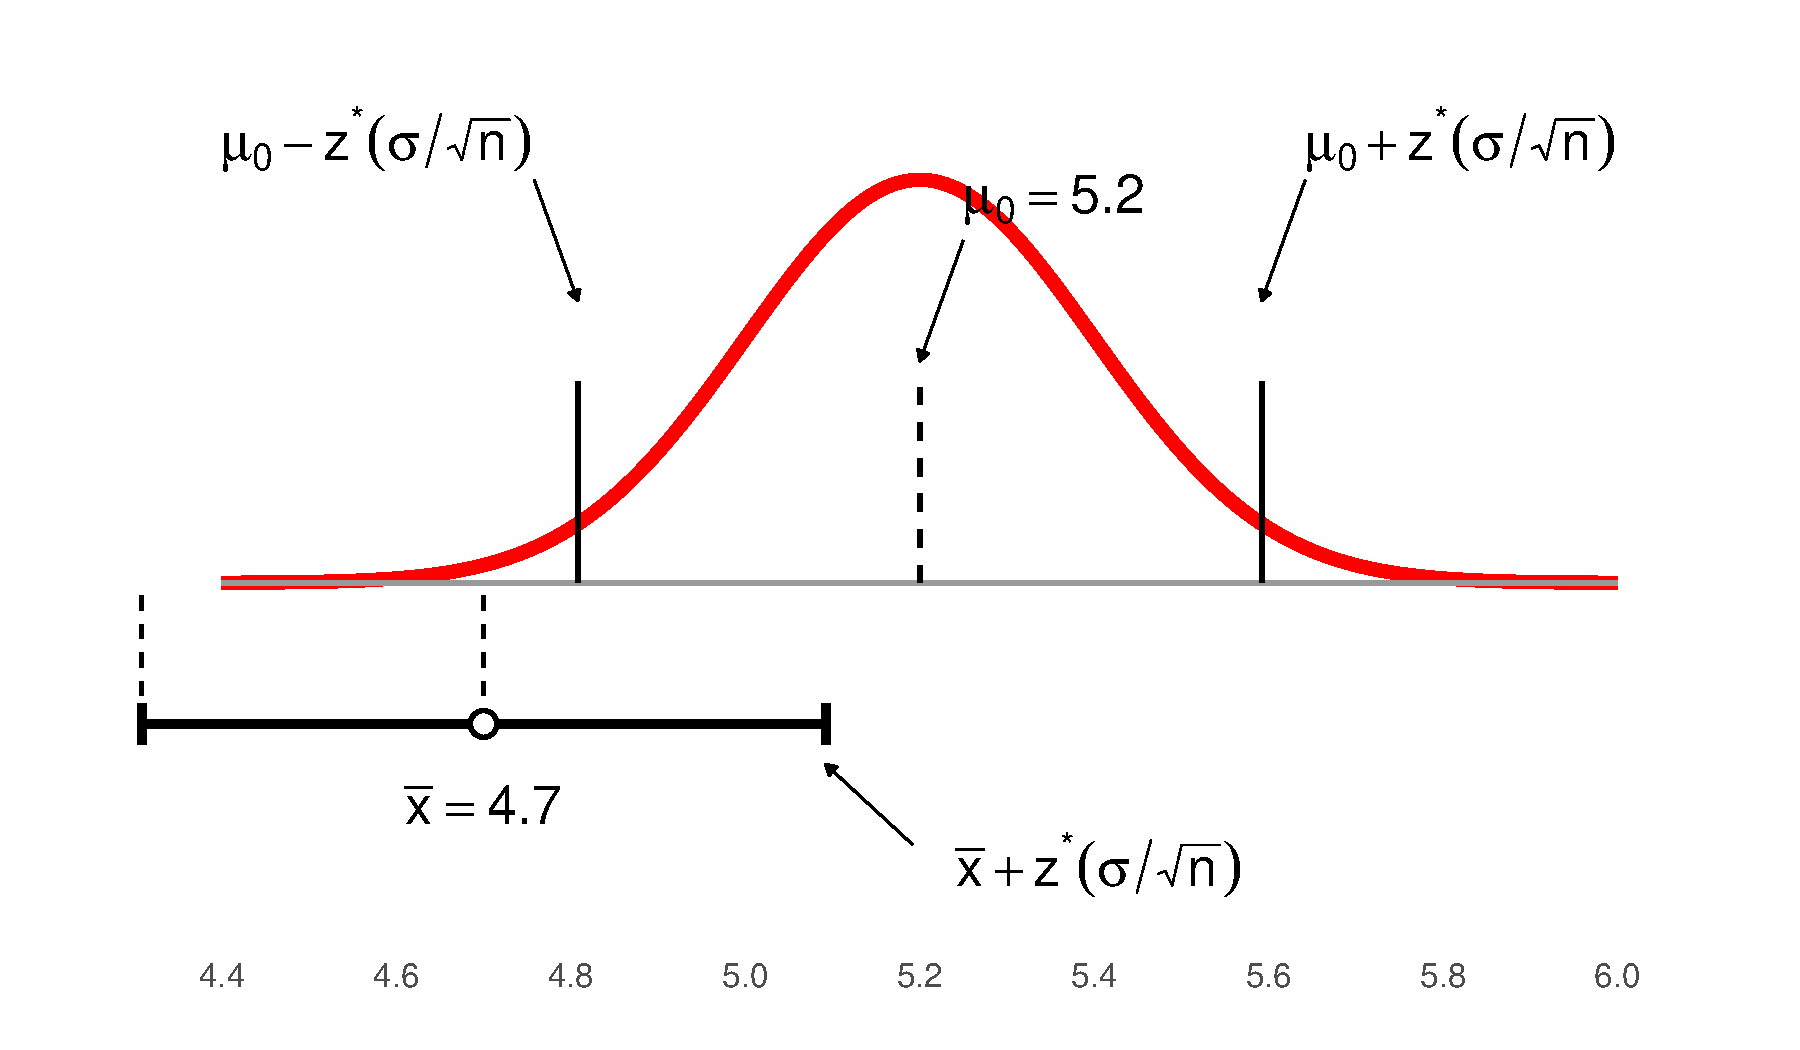
\includegraphics[keepaspectratio]{index_files/figure-pdf/fig-ci-hypothesis-connection-1.pdf}}

}

\caption{\label{fig-ci-hypothesis-connection}Relationship between
confidence intervals and hypothesis tests}

\end{figure}%

\bookmarksetup{startatroot}

\chapter{Chapter 11: Inference About a Population
Mean}\label{chapter-11-inference-about-a-population-mean}

Before conducting statistical inference about a population mean, we must
verify that certain conditions are met:

\begin{itemize}
\item
  We can regard our sample as a simple random sample (SRS).
\item
  The population is Normal, so that the sampling distribution of
  \(\bar{x}\) is also Normal.

  \begin{itemize}
  \tightlist
  \item
    Alternatively, the population is very large, and the sample size is
    large enough that the sampling distribution is approximately Normal,
    because of the Central Limit Theorem. (Our previous rules of thumb
    of \(n\) greater than 25 or 40 will be modified later in the
    chapter.)
  \end{itemize}
\item
  Both \(\mu\) and \(\sigma\) are unknown parameters.
\end{itemize}

Our goal, of course, is to estimate \(\mu\).

\section{\texorpdfstring{Inference About \(\mu\) When \(\sigma\) Is
Unknown}{Inference About \textbackslash mu When \textbackslash sigma Is Unknown}}\label{inference-about-mu-when-sigma-is-unknown}

Thus far we've assumed we know \(\sigma\), the population standard
deviation.

But this is unrealistic, given that we don't even know \(\mu\), the mean
we are trying to estimate.

What if we do not know \(\sigma\)?

We use the sample estimate, \(s\), to replace \(\sigma\) in our
formulas.

Mathematical analysis shows that this is an acceptable substitution.

However, making the substitution requires some changes to our
procedures.

In particular, we have to use a new probability distribution for our
significance tests and confidence intervals, the \emph{t} distribution.

\section{\texorpdfstring{When \(\sigma\) Is
Unknown}{When \textbackslash sigma Is Unknown}}\label{when-sigma-is-unknown}

In an SRS, the distribution of the cases in a sample echoes the
distribution in the population, but the \emph{correspondence gets better
in larger samples}:

\begin{Shaded}
\begin{Highlighting}[]
\FunctionTok{suppressPackageStartupMessages}\NormalTok{(\{}
  \FunctionTok{library}\NormalTok{(ggplot2)}
  \FunctionTok{library}\NormalTok{(dplyr)}
  \FunctionTok{library}\NormalTok{(tibble)}
  \FunctionTok{library}\NormalTok{(grid)   }\CommentTok{\# unit(), arrow()}
\NormalTok{\})}

\FunctionTok{set.seed}\NormalTok{(}\DecValTok{123}\NormalTok{)}

\CommentTok{\# {-}{-}{-}{-}{-} Population {-}{-}{-}{-}{-}}
\NormalTok{mu    }\OtherTok{\textless{}{-}} \DecValTok{30}
\NormalTok{sigma }\OtherTok{\textless{}{-}} \DecValTok{10}

\CommentTok{\# {-}{-}{-}{-}{-} Samples {-}{-}{-}{-}{-}}
\NormalTok{n1 }\OtherTok{\textless{}{-}} \DecValTok{20}\NormalTok{;  n2 }\OtherTok{\textless{}{-}} \DecValTok{200}
\NormalTok{samp1 }\OtherTok{\textless{}{-}} \FunctionTok{rnorm}\NormalTok{(n1, }\AttributeTok{mean =}\NormalTok{ mu, }\AttributeTok{sd =}\NormalTok{ sigma)}
\NormalTok{samp2 }\OtherTok{\textless{}{-}} \FunctionTok{rnorm}\NormalTok{(n2, }\AttributeTok{mean =}\NormalTok{ mu, }\AttributeTok{sd =}\NormalTok{ sigma)}

\NormalTok{xbar1 }\OtherTok{\textless{}{-}} \FunctionTok{mean}\NormalTok{(samp1); s1 }\OtherTok{\textless{}{-}} \FunctionTok{sd}\NormalTok{(samp1)}
\NormalTok{xbar2 }\OtherTok{\textless{}{-}} \FunctionTok{mean}\NormalTok{(samp2); s2 }\OtherTok{\textless{}{-}} \FunctionTok{sd}\NormalTok{(samp2)}

\CommentTok{\# {-}{-}{-}{-}{-} Curve data (same Normal, duplicated per panel) {-}{-}{-}{-}{-}}
\NormalTok{x\_vals }\OtherTok{\textless{}{-}} \FunctionTok{seq}\NormalTok{(}\DecValTok{0}\NormalTok{, }\DecValTok{60}\NormalTok{, }\AttributeTok{length.out =} \DecValTok{600}\NormalTok{)}
\NormalTok{y\_vals }\OtherTok{\textless{}{-}} \FunctionTok{dnorm}\NormalTok{(x\_vals, }\AttributeTok{mean =}\NormalTok{ mu, }\AttributeTok{sd =}\NormalTok{ sigma)}
\NormalTok{y\_max  }\OtherTok{\textless{}{-}} \FunctionTok{max}\NormalTok{(y\_vals)}

\NormalTok{lab\_small }\OtherTok{\textless{}{-}} \StringTok{"n = 20"}
\NormalTok{lab\_large }\OtherTok{\textless{}{-}} \StringTok{"n = 200"}

\NormalTok{df\_curve }\OtherTok{\textless{}{-}} \FunctionTok{bind\_rows}\NormalTok{(}
  \FunctionTok{tibble}\NormalTok{(}\AttributeTok{panel =}\NormalTok{ lab\_small, }\AttributeTok{x =}\NormalTok{ x\_vals, }\AttributeTok{y =}\NormalTok{ y\_vals),}
  \FunctionTok{tibble}\NormalTok{(}\AttributeTok{panel =}\NormalTok{ lab\_large, }\AttributeTok{x =}\NormalTok{ x\_vals, }\AttributeTok{y =}\NormalTok{ y\_vals)}
\NormalTok{)}

\CommentTok{\# {-}{-}{-}{-}{-} Build a dense baseline "swarm" WITHOUT extra packages {-}{-}{-}{-}{-}}
\CommentTok{\# We bin x, then spread points within each bin so they don\textquotesingle{}t overplot.}
\NormalTok{mk\_baseline\_swarm }\OtherTok{\textless{}{-}} \ControlFlowTok{function}\NormalTok{(values, panel, }\AttributeTok{binwidth =} \FloatTok{0.6}\NormalTok{, }\AttributeTok{band\_y =} \FloatTok{0.0007}\NormalTok{,}
                              \AttributeTok{max\_half\_width =} \FloatTok{0.45}\NormalTok{, }\AttributeTok{vstep =} \FloatTok{0.00005}\NormalTok{,}
                              \AttributeTok{size =} \FloatTok{1.2}\NormalTok{, }\AttributeTok{alpha =} \FloatTok{0.95}\NormalTok{) \{}
  \CommentTok{\# Bin index and bin center}
\NormalTok{  b }\OtherTok{\textless{}{-}} \FunctionTok{floor}\NormalTok{(values }\SpecialCharTok{/}\NormalTok{ binwidth)}
  \FunctionTok{tibble}\NormalTok{(}\AttributeTok{panel =}\NormalTok{ panel, }\AttributeTok{value =}\NormalTok{ values, }\AttributeTok{bin =}\NormalTok{ b) }\SpecialCharTok{|\textgreater{}}
    \FunctionTok{group\_by}\NormalTok{(panel, bin) }\SpecialCharTok{|\textgreater{}}
    \FunctionTok{mutate}\NormalTok{(}
      \AttributeTok{n\_in\_bin =} \FunctionTok{n}\NormalTok{(),}
      \AttributeTok{rank\_in\_bin =} \FunctionTok{row\_number}\NormalTok{(),}
      \CommentTok{\# spread symmetrically within [{-}max\_half\_width, +max\_half\_width] * binwidth}
      \AttributeTok{x\_offset =} \FunctionTok{ifelse}\NormalTok{(}
\NormalTok{        n\_in\_bin }\SpecialCharTok{==} \DecValTok{1}\NormalTok{,}
        \DecValTok{0}\NormalTok{,}
\NormalTok{        ((rank\_in\_bin }\SpecialCharTok{{-}}\NormalTok{ (n\_in\_bin }\SpecialCharTok{+} \DecValTok{1}\NormalTok{)}\SpecialCharTok{/}\DecValTok{2}\NormalTok{) }\SpecialCharTok{/}\NormalTok{ ((n\_in\_bin }\SpecialCharTok{{-}} \DecValTok{1}\NormalTok{)}\SpecialCharTok{/}\DecValTok{2}\NormalTok{)) }\SpecialCharTok{*}\NormalTok{ max\_half\_width }\SpecialCharTok{*}\NormalTok{ binwidth}
\NormalTok{      ),}
      \AttributeTok{x\_swarm =}\NormalTok{ (bin }\SpecialCharTok{+} \FloatTok{0.5}\NormalTok{) }\SpecialCharTok{*}\NormalTok{ binwidth }\SpecialCharTok{+}\NormalTok{ x\_offset,}
      \CommentTok{\# thin vertical band so labels below aren\textquotesingle{}t crowded}
      \AttributeTok{y\_swarm =}\NormalTok{ band\_y }\SpecialCharTok{+}\NormalTok{ ((rank\_in\_bin }\SpecialCharTok{{-}} \DecValTok{1}\NormalTok{) }\SpecialCharTok{\%\%} \DecValTok{7} \SpecialCharTok{{-}} \DecValTok{3}\NormalTok{) }\SpecialCharTok{*}\NormalTok{ vstep,}
      \AttributeTok{size  =}\NormalTok{ size,}
      \AttributeTok{alpha =}\NormalTok{ alpha,}
      \AttributeTok{col   =} \StringTok{"\#111111"}
\NormalTok{    ) }\SpecialCharTok{|\textgreater{}}
    \FunctionTok{ungroup}\NormalTok{()}
\NormalTok{\}}

\CommentTok{\# n=20: modest spread \& bigger dots; n=200: much tighter band but MANY dots}
\NormalTok{df\_samp }\OtherTok{\textless{}{-}} \FunctionTok{bind\_rows}\NormalTok{(}
  \FunctionTok{mk\_baseline\_swarm}\NormalTok{(samp1, lab\_small, }\AttributeTok{binwidth =} \FloatTok{1.0}\NormalTok{, }\AttributeTok{size =} \FloatTok{1.8}\NormalTok{, }\AttributeTok{alpha =} \FloatTok{0.95}\NormalTok{),}
  \FunctionTok{mk\_baseline\_swarm}\NormalTok{(samp2, lab\_large, }\AttributeTok{binwidth =} \FloatTok{0.6}\NormalTok{, }\AttributeTok{size =} \FloatTok{0.6}\NormalTok{, }\AttributeTok{alpha =} \FloatTok{1.00}\NormalTok{)}
\NormalTok{)}

\CommentTok{\# Baseline at y=0}
\NormalTok{df\_base }\OtherTok{\textless{}{-}} \FunctionTok{tibble}\NormalTok{(}
  \AttributeTok{panel =} \FunctionTok{c}\NormalTok{(lab\_small, lab\_large),}
  \AttributeTok{x =} \DecValTok{0}\NormalTok{, }\AttributeTok{xend =} \DecValTok{60}\NormalTok{, }\AttributeTok{y =} \DecValTok{0}\NormalTok{, }\AttributeTok{yend =} \DecValTok{0}
\NormalTok{)}

\CommentTok{\# Arrows to the curve}
\NormalTok{df\_arrows }\OtherTok{\textless{}{-}} \FunctionTok{tribble}\NormalTok{(}
  \SpecialCharTok{\textasciitilde{}}\NormalTok{panel,      }\SpecialCharTok{\textasciitilde{}}\NormalTok{x,  }\SpecialCharTok{\textasciitilde{}}\NormalTok{xend, }\SpecialCharTok{\textasciitilde{}}\NormalTok{y,                  }\SpecialCharTok{\textasciitilde{}}\NormalTok{yend,}
\NormalTok{  lab\_small,   }\DecValTok{18}\NormalTok{,    }\DecValTok{25}\NormalTok{,   y\_max}\SpecialCharTok{*}\FloatTok{0.75}\NormalTok{,         y\_max}\SpecialCharTok{*}\FloatTok{0.92}\NormalTok{,}
\NormalTok{  lab\_large,   }\DecValTok{42}\NormalTok{,    }\DecValTok{35}\NormalTok{,   y\_max}\SpecialCharTok{*}\FloatTok{0.75}\NormalTok{,         y\_max}\SpecialCharTok{*}\FloatTok{0.92}
\NormalTok{)}

\CommentTok{\# Bottom statistics (plotmath), placed below baseline}
\NormalTok{stat\_y }\OtherTok{\textless{}{-}} \SpecialCharTok{{-}}\FloatTok{0.006}
\NormalTok{df\_stats }\OtherTok{\textless{}{-}} \FunctionTok{tribble}\NormalTok{(}
  \SpecialCharTok{\textasciitilde{}}\NormalTok{panel,      }\SpecialCharTok{\textasciitilde{}}\NormalTok{x, }\SpecialCharTok{\textasciitilde{}}\NormalTok{y,       }\SpecialCharTok{\textasciitilde{}}\NormalTok{lab,}
\NormalTok{  lab\_small,   }\DecValTok{30}\NormalTok{, stat\_y, }\FunctionTok{sprintf}\NormalTok{(}\StringTok{"n==\%d\textasciitilde{}\textasciitilde{}bar(x)==\%.1f\textasciitilde{}\textasciitilde{}s==\%.2f"}\NormalTok{, n1, xbar1, s1),}
\NormalTok{  lab\_large,   }\DecValTok{30}\NormalTok{, stat\_y, }\FunctionTok{sprintf}\NormalTok{(}\StringTok{"n==\%d\textasciitilde{}\textasciitilde{}bar(x)==\%.1f\textasciitilde{}\textasciitilde{}s==\%.2f"}\NormalTok{, n2, xbar2, s2)}
\NormalTok{)}

\FunctionTok{ggplot}\NormalTok{() }\SpecialCharTok{+}
  \CommentTok{\# baseline}
  \FunctionTok{geom\_segment}\NormalTok{(}\AttributeTok{data =}\NormalTok{ df\_base,}
               \FunctionTok{aes}\NormalTok{(}\AttributeTok{x =}\NormalTok{ x, }\AttributeTok{xend =}\NormalTok{ xend, }\AttributeTok{y =}\NormalTok{ y, }\AttributeTok{yend =}\NormalTok{ yend),}
               \AttributeTok{color =} \StringTok{"gray60"}\NormalTok{, }\AttributeTok{linewidth =} \FloatTok{0.9}\NormalTok{) }\SpecialCharTok{+}
  \CommentTok{\# red population curve}
  \FunctionTok{geom\_line}\NormalTok{(}\AttributeTok{data =}\NormalTok{ df\_curve, }\FunctionTok{aes}\NormalTok{(x, y), }\AttributeTok{color =} \StringTok{"red"}\NormalTok{, }\AttributeTok{linewidth =} \FloatTok{2.6}\NormalTok{) }\SpecialCharTok{+}
  \CommentTok{\# SWARMED rugs (n=200 now shows a LOT more dots)}
  \FunctionTok{geom\_point}\NormalTok{(}\AttributeTok{data =}\NormalTok{ df\_samp,}
             \FunctionTok{aes}\NormalTok{(}\AttributeTok{x =}\NormalTok{ x\_swarm, }\AttributeTok{y =}\NormalTok{ y\_swarm, }\AttributeTok{size =}\NormalTok{ size, }\AttributeTok{alpha =}\NormalTok{ alpha, }\AttributeTok{color =}\NormalTok{ col),}
             \AttributeTok{shape =} \DecValTok{16}\NormalTok{, }\AttributeTok{show.legend =} \ConstantTok{FALSE}\NormalTok{) }\SpecialCharTok{+}
  \FunctionTok{scale\_color\_identity}\NormalTok{() }\SpecialCharTok{+}
  \FunctionTok{scale\_size\_identity}\NormalTok{() }\SpecialCharTok{+}
  \FunctionTok{scale\_alpha\_identity}\NormalTok{() }\SpecialCharTok{+}
  \CommentTok{\# arrows}
  \FunctionTok{geom\_segment}\NormalTok{(}\AttributeTok{data =}\NormalTok{ df\_arrows,}
               \FunctionTok{aes}\NormalTok{(}\AttributeTok{x =}\NormalTok{ x, }\AttributeTok{xend =}\NormalTok{ xend, }\AttributeTok{y =}\NormalTok{ y, }\AttributeTok{yend =}\NormalTok{ yend),}
               \AttributeTok{arrow =} \FunctionTok{arrow}\NormalTok{(}\AttributeTok{length =} \FunctionTok{unit}\NormalTok{(}\FloatTok{0.35}\NormalTok{, }\StringTok{"cm"}\NormalTok{), }\AttributeTok{type =} \StringTok{"closed"}\NormalTok{),}
               \AttributeTok{linewidth =} \FloatTok{0.8}\NormalTok{, }\AttributeTok{color =} \StringTok{"black"}\NormalTok{) }\SpecialCharTok{+}
  \CommentTok{\# bottom stats (bold math)}
  \FunctionTok{geom\_text}\NormalTok{(}\AttributeTok{data =}\NormalTok{ df\_stats,}
            \FunctionTok{aes}\NormalTok{(}\AttributeTok{x =}\NormalTok{ x, }\AttributeTok{y =}\NormalTok{ y, }\AttributeTok{label =}\NormalTok{ lab),}
            \AttributeTok{parse =} \ConstantTok{TRUE}\NormalTok{, }\AttributeTok{fontface =} \StringTok{"bold"}\NormalTok{, }\AttributeTok{size =} \FloatTok{5.2}\NormalTok{) }\SpecialCharTok{+}
  \FunctionTok{facet\_wrap}\NormalTok{(}\SpecialCharTok{\textasciitilde{}}\NormalTok{ panel, }\AttributeTok{ncol =} \DecValTok{2}\NormalTok{) }\SpecialCharTok{+}
  \FunctionTok{scale\_x\_continuous}\NormalTok{(}\AttributeTok{limits =} \FunctionTok{c}\NormalTok{(}\DecValTok{0}\NormalTok{, }\DecValTok{60}\NormalTok{), }\AttributeTok{breaks =} \FunctionTok{seq}\NormalTok{(}\DecValTok{0}\NormalTok{, }\DecValTok{60}\NormalTok{, }\DecValTok{20}\NormalTok{)) }\SpecialCharTok{+}
  \FunctionTok{coord\_cartesian}\NormalTok{(}\AttributeTok{ylim =} \FunctionTok{c}\NormalTok{(}\SpecialCharTok{{-}}\FloatTok{0.008}\NormalTok{, y\_max }\SpecialCharTok{*} \FloatTok{1.05}\NormalTok{), }\AttributeTok{clip =} \StringTok{"off"}\NormalTok{) }\SpecialCharTok{+}
  \FunctionTok{labs}\NormalTok{(}
    \AttributeTok{title =} \FunctionTok{bquote}\NormalTok{(}\StringTok{"Normal population:"} \SpecialCharTok{\textasciitilde{}}\NormalTok{ mu }\SpecialCharTok{==}\NormalTok{ .(mu) }\SpecialCharTok{*} \StringTok{","} \SpecialCharTok{\textasciitilde{}}\NormalTok{ sigma }\SpecialCharTok{==}\NormalTok{ .(sigma)),}
    \AttributeTok{x =} \ConstantTok{NULL}\NormalTok{, }\AttributeTok{y =} \ConstantTok{NULL}
\NormalTok{  ) }\SpecialCharTok{+}
  \FunctionTok{theme\_minimal}\NormalTok{(}\AttributeTok{base\_size =} \DecValTok{16}\NormalTok{) }\SpecialCharTok{+}
  \FunctionTok{theme}\NormalTok{(}
    \AttributeTok{plot.title   =} \FunctionTok{element\_text}\NormalTok{(}\AttributeTok{face =} \StringTok{"bold"}\NormalTok{),}
    \AttributeTok{panel.grid   =} \FunctionTok{element\_blank}\NormalTok{(),}
    \AttributeTok{axis.text.x  =} \FunctionTok{element\_text}\NormalTok{(}\AttributeTok{size =} \DecValTok{13}\NormalTok{, }\AttributeTok{color =} \StringTok{"black"}\NormalTok{),}
    \AttributeTok{axis.text.y  =} \FunctionTok{element\_blank}\NormalTok{(),}
    \AttributeTok{axis.ticks.y =} \FunctionTok{element\_blank}\NormalTok{(),}
    \AttributeTok{axis.ticks.x =} \FunctionTok{element\_line}\NormalTok{(}\AttributeTok{color =} \StringTok{"black"}\NormalTok{),}
    \AttributeTok{panel.background =} \FunctionTok{element\_rect}\NormalTok{(}\AttributeTok{fill =} \StringTok{"white"}\NormalTok{, }\AttributeTok{color =} \ConstantTok{NA}\NormalTok{),}
    \AttributeTok{plot.background  =} \FunctionTok{element\_rect}\NormalTok{(}\AttributeTok{fill =} \StringTok{"white"}\NormalTok{, }\AttributeTok{color =} \ConstantTok{NA}\NormalTok{),}
    \AttributeTok{plot.margin      =} \FunctionTok{margin}\NormalTok{(}\DecValTok{8}\NormalTok{, }\DecValTok{16}\NormalTok{, }\DecValTok{36}\NormalTok{, }\DecValTok{16}\NormalTok{)}
\NormalTok{  )}
\end{Highlighting}
\end{Shaded}

\begin{figure}[H]

\centering{

\pandocbounded{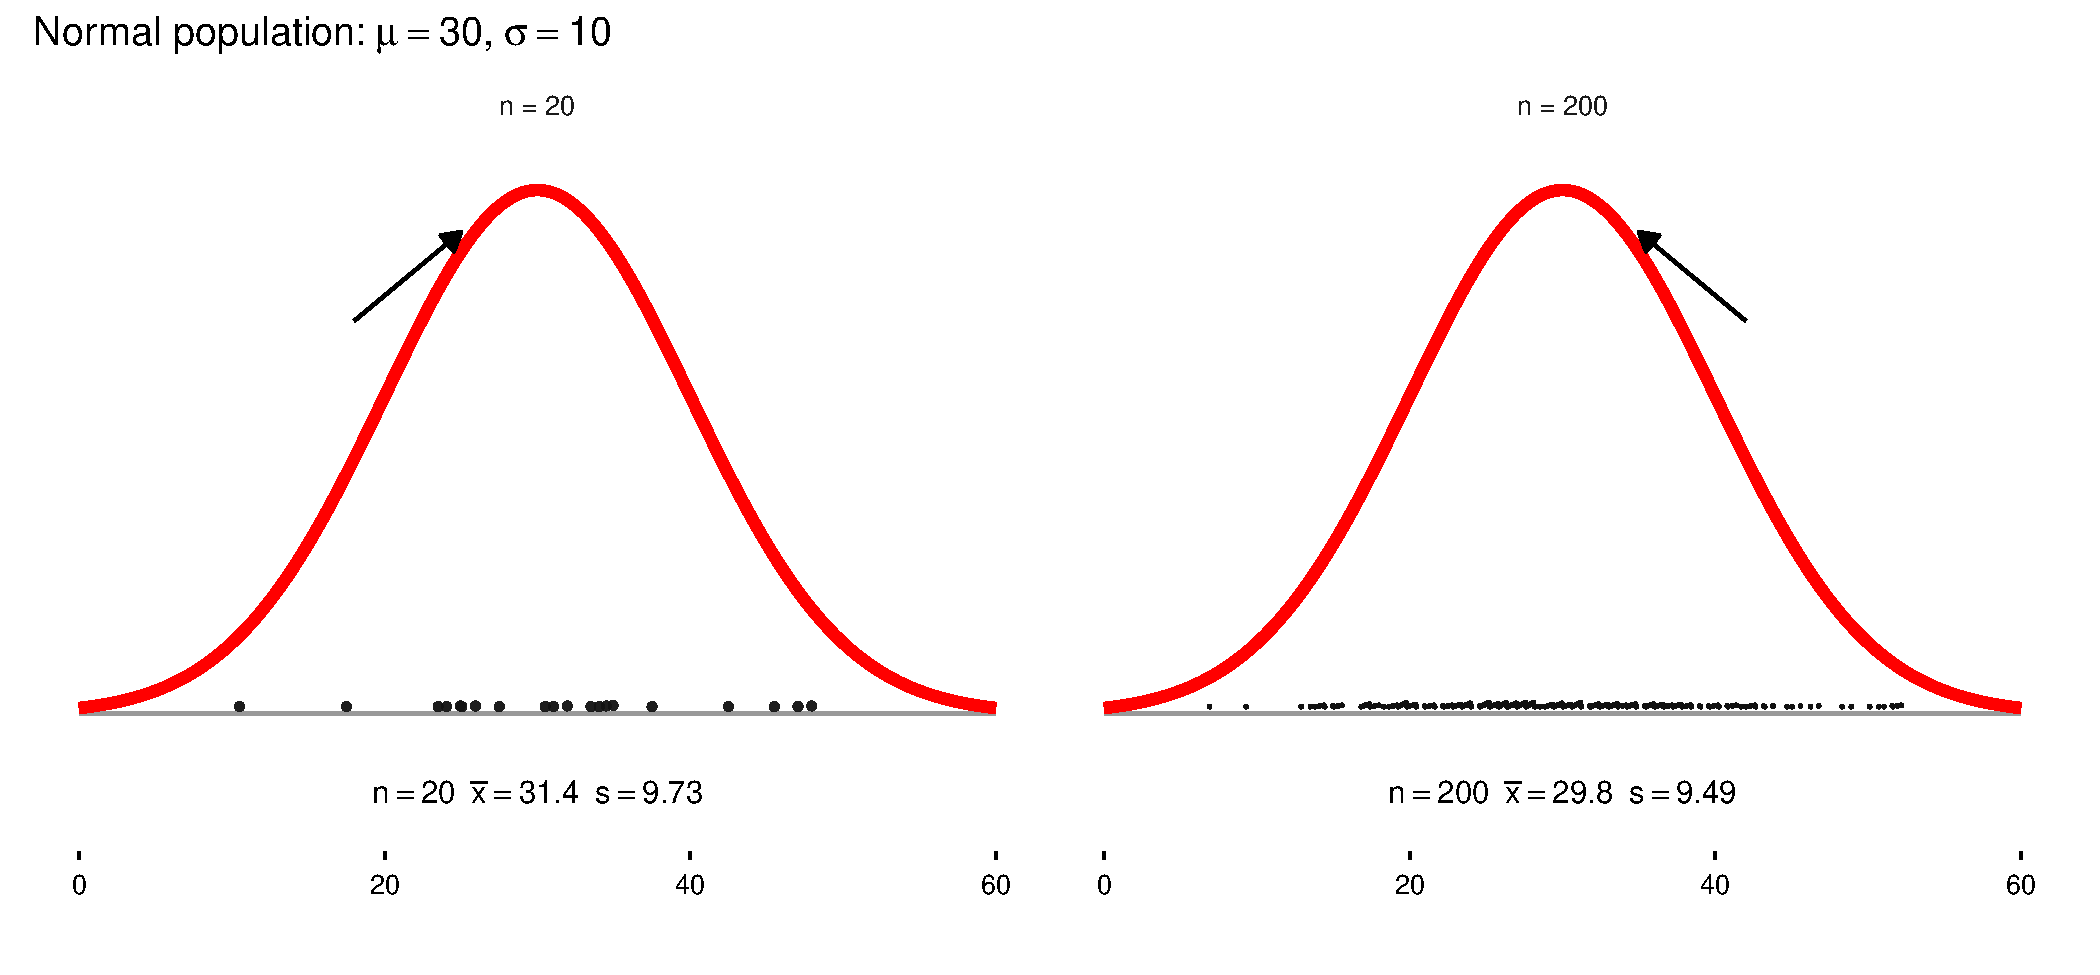
\includegraphics[keepaspectratio]{index_files/figure-pdf/fig-sampling-correspondence-sexy-1.pdf}}

}

\caption{\label{fig-sampling-correspondence-sexy}Comparison of sample
distributions for different sample sizes from a Normal population.}

\end{figure}%

\section{Modern Statistics and the Great
Substitution}\label{modern-statistics-and-the-great-substitution}

Wm. Gossett, a Guinness research mathematician, saw that when \(s\) is
substituted for \(\sigma\) in the \(z\) formula, like this:

\[
\frac{\bar{x} - \mu_0}{s/\sqrt{n}}
\]

the result is no longer normally distributed.

The new distribution is called \emph{t} rather than \emph{z}. That is,

\[
t = \frac{\bar{x} - \mu_0}{s/\sqrt{n}}
\]

The distribution of \(t\) is like the normal distribution, but with
longer tails.

The difference between the two distributions was enough to give Guinness
Brewery a competitive advantage.

\section{\texorpdfstring{What Makes \(t\) Different from
\(z\)}{What Makes t Different from z}}\label{what-makes-t-different-from-z}

Though the formulas are almost the same, the formula for \(z\) involves
dividing a Normally-distributed quantity, namely \(\bar{x}\), by a
\emph{constant}, \(\sigma/\sqrt{n}\):

\[
z = \frac{\bar{x} - \mu_0}{\sigma/\sqrt{n}}
\]

(Normally distributed, that is, if the sampling distribution is Normal.)

But the similar formula for \(t\) divides the Normally-distributed
\(\bar{x}\) by another Normally-distributed quantity, namely,
\(s/\sqrt{n}\):

\[
t = \frac{\bar{x} - \mu_0}{s/\sqrt{n}}
\]

Intuitively, since the denominator for \(t\) is less stable, the
resulting quantity has the \emph{longer-tailed} distribution called the
\(t\) distribution.

\section{\texorpdfstring{\(t\)
Distributions}{t Distributions}}\label{t-distributions}

All \(t\) distributions have the same mean, namely, zero.

But there are an infinite number of \(t\) distributions, each with a
different spread and shape.

These distributions are determined by (or ``indexed by'') a number
called the \emph{degrees of freedom}.

In the problems we are dealing with, the appropriate degrees of freedom
value is given by \(n - 1\), where \(n\) is the sample size:

\[
df = n - 1
\]

\section{\texorpdfstring{Example \(t\)
Distributions}{Example t Distributions}}\label{example-t-distributions}

As the degrees of freedom \emph{increase}, the \(t\) distribution
becomes \emph{less} spread out, and its shape approaches the Normal
distribution.

Beyond some point, say \(df = 120\), the two distributions are
practically the same.

\section{Modern Statistics and the Great
Substitution}\label{modern-statistics-and-the-great-substitution-1}

Wm. Gossett, a Guinness research mathematician, saw that when \(s\) is
substituted for \(\sigma\) in the \(z\) formula, like this:

\[
\frac{\bar{x} - \mu_0}{s/\sqrt{n}}
\]

the result is no longer normally distributed.

The new distribution is called \emph{t} rather than \emph{z}. That is,

\[
t = \frac{\bar{x} - \mu_0}{s/\sqrt{n}}
\]

The distribution of \(t\) is like the normal distribution, but with
longer tails.

The difference between the two distributions was enough to give Guinness
Brewery a competitive advantage.

\section{\texorpdfstring{What Makes \(t\) Different from
\(z\)}{What Makes t Different from z}}\label{what-makes-t-different-from-z-1}

Though the formulas are almost the same, the formula for \(z\) involves
dividing a Normally-distributed quantity, namely \(\bar{x}\), by a
\emph{constant}, \(\sigma/\sqrt{n}\):

\[
z = \frac{\bar{x} - \mu_0}{\sigma/\sqrt{n}}
\]

(Normally distributed, that is, if the sampling distribution is Normal.)

But the similar formula for \(t\) divides the Normally-distributed
\(\bar{x}\) by another Normally-distributed quantity, namely,
\(s/\sqrt{n}\):

\[
t = \frac{\bar{x} - \mu_0}{s/\sqrt{n}}
\]

Intuitively, since the denominator for \(t\) is less stable, the
resulting quantity has the \emph{longer-tailed} distribution called the
\(t\) distribution.

\section{\texorpdfstring{\(t\)
Distributions}{t Distributions}}\label{t-distributions-1}

All \(t\) distributions have the same mean, namely, zero.

But there are an infinite number of \(t\) distributions, each with a
different spread and shape.

These distributions are determined by (or ``indexed by'') a number
called the \emph{degrees of freedom}.

In the problems we are dealing with, the appropriate degrees of freedom
value is given by \(n - 1\), where \(n\) is the sample size:

\[
df = n - 1
\]

\section{\texorpdfstring{Example \(t\)
Distributions}{Example t Distributions}}\label{example-t-distributions-1}

As the degrees of freedom \emph{increase}, the \(t\) distribution
becomes \emph{less} spread out, and its shape approaches the Normal
distribution.

Beyond some point, say \(df = 120\), the two distributions are
practically the same.

It is crucial to note that in the graph below, the solid curve in the
graph is the standard Normal distribution, which is the familiar
bell-shaped curve you have seen in statistics many times. The two dashed
and dotted curves are t-distributions, which look similar but have
fatter (heavier) tails --- meaning they place more probability on more
extreme values far from the center. This matters in practice because
when sample sizes are small, our estimates are more variable/uncertain,
so the t-distribution allows for more room in the tails to account for
that extra uncertainty.

As the sample size increases, the t-distribution gets closer and closer
to the Normal curve (notice how the dotted line with 9 degrees of
freedom is already much closer than the dashed line with only 2). This
is why in large samples (e.g., n\textgreater30), using the Normal
approximation is usually fine --- because the t-distribution has already
``converged'' to the Normal shape. But when samples are small, the
t-distribution protects us from being overconfident by widening the
tails and making us more cautious in our conclusions.

\begin{Shaded}
\begin{Highlighting}[]
\FunctionTok{library}\NormalTok{(ggplot2)}

\CommentTok{\# Create x values}
\NormalTok{x }\OtherTok{\textless{}{-}} \FunctionTok{seq}\NormalTok{(}\SpecialCharTok{{-}}\DecValTok{4}\NormalTok{, }\DecValTok{4}\NormalTok{, }\AttributeTok{length.out =} \DecValTok{500}\NormalTok{)}

\CommentTok{\# Create data frame with all distributions}
\NormalTok{df\_distributions }\OtherTok{\textless{}{-}} \FunctionTok{data.frame}\NormalTok{(}
  \AttributeTok{x =} \FunctionTok{rep}\NormalTok{(x, }\DecValTok{3}\NormalTok{),}
  \AttributeTok{density =} \FunctionTok{c}\NormalTok{(}
    \FunctionTok{dt}\NormalTok{(x, }\AttributeTok{df =} \DecValTok{2}\NormalTok{),}
    \FunctionTok{dt}\NormalTok{(x, }\AttributeTok{df =} \DecValTok{9}\NormalTok{),}
    \FunctionTok{dnorm}\NormalTok{(x)}
\NormalTok{  ),}
  \AttributeTok{distribution =} \FunctionTok{rep}\NormalTok{(}
    \FunctionTok{c}\NormalTok{(}\StringTok{"t, 2 degrees of freedom"}\NormalTok{, }
      \StringTok{"t, 9 degrees of freedom"}\NormalTok{, }
      \StringTok{"standard Normal"}\NormalTok{),}
    \AttributeTok{each =} \FunctionTok{length}\NormalTok{(x)}
\NormalTok{  )}
\NormalTok{)}

\CommentTok{\# Create the plot}
\FunctionTok{ggplot}\NormalTok{(df\_distributions, }\FunctionTok{aes}\NormalTok{(}\AttributeTok{x =}\NormalTok{ x, }\AttributeTok{y =}\NormalTok{ density, }
                              \AttributeTok{color =}\NormalTok{ distribution, }
                              \AttributeTok{linetype =}\NormalTok{ distribution)) }\SpecialCharTok{+}
  \FunctionTok{geom\_line}\NormalTok{(}\AttributeTok{linewidth =} \FloatTok{1.3}\NormalTok{) }\SpecialCharTok{+}
  
  \CommentTok{\# Vertical line at 0}
  \FunctionTok{geom\_vline}\NormalTok{(}\AttributeTok{xintercept =} \DecValTok{0}\NormalTok{, }\AttributeTok{color =} \StringTok{"gray50"}\NormalTok{, }\AttributeTok{linewidth =} \FloatTok{0.8}\NormalTok{) }\SpecialCharTok{+}
  
  \CommentTok{\# Add annotation about heavier tails}
  \FunctionTok{annotate}\NormalTok{(}\StringTok{"text"}\NormalTok{, }\AttributeTok{x =} \SpecialCharTok{{-}}\FloatTok{3.5}\NormalTok{, }\AttributeTok{y =} \FloatTok{0.35}\NormalTok{,}
           \AttributeTok{label =} \StringTok{"t distributions have more}\SpecialCharTok{\textbackslash{}n}\StringTok{area in the tails than the}\SpecialCharTok{\textbackslash{}n}\StringTok{standard Normal distribution"}\NormalTok{,}
           \AttributeTok{hjust =} \DecValTok{0}\NormalTok{, }\AttributeTok{size =} \DecValTok{4}\NormalTok{, }\AttributeTok{lineheight =} \FloatTok{0.9}\NormalTok{, }\AttributeTok{color =} \StringTok{"black"}\NormalTok{) }\SpecialCharTok{+}
  
  \CommentTok{\# Styling}
  \FunctionTok{scale\_color\_manual}\NormalTok{(}\AttributeTok{values =} \FunctionTok{c}\NormalTok{(}
    \StringTok{"t, 2 degrees of freedom"} \OtherTok{=} \StringTok{"\#E41A1C"}\NormalTok{,}
    \StringTok{"t, 9 degrees of freedom"} \OtherTok{=} \StringTok{"\#E41A1C"}\NormalTok{,}
    \StringTok{"standard Normal"} \OtherTok{=} \StringTok{"\#E41A1C"}
\NormalTok{  )) }\SpecialCharTok{+}
  \FunctionTok{scale\_linetype\_manual}\NormalTok{(}\AttributeTok{values =} \FunctionTok{c}\NormalTok{(}
    \StringTok{"t, 2 degrees of freedom"} \OtherTok{=} \StringTok{"dashed"}\NormalTok{,}
    \StringTok{"t, 9 degrees of freedom"} \OtherTok{=} \StringTok{"dotted"}\NormalTok{,}
    \StringTok{"standard Normal"} \OtherTok{=} \StringTok{"solid"}
\NormalTok{  )) }\SpecialCharTok{+}
  
  \FunctionTok{scale\_x\_continuous}\NormalTok{(}\AttributeTok{breaks =} \FunctionTok{seq}\NormalTok{(}\SpecialCharTok{{-}}\DecValTok{4}\NormalTok{, }\DecValTok{4}\NormalTok{, }\AttributeTok{by =} \DecValTok{1}\NormalTok{)) }\SpecialCharTok{+}
  \FunctionTok{scale\_y\_continuous}\NormalTok{(}\AttributeTok{limits =} \FunctionTok{c}\NormalTok{(}\DecValTok{0}\NormalTok{, }\FloatTok{0.42}\NormalTok{), }\AttributeTok{expand =} \FunctionTok{c}\NormalTok{(}\DecValTok{0}\NormalTok{, }\DecValTok{0}\NormalTok{)) }\SpecialCharTok{+}
  
  \FunctionTok{labs}\NormalTok{(}
    \AttributeTok{x =} \StringTok{""}\NormalTok{,}
    \AttributeTok{y =} \StringTok{""}\NormalTok{,}
    \AttributeTok{color =} \StringTok{""}\NormalTok{,}
    \AttributeTok{linetype =} \StringTok{""}
\NormalTok{  ) }\SpecialCharTok{+}
  
  \FunctionTok{theme\_minimal}\NormalTok{(}\AttributeTok{base\_size =} \DecValTok{13}\NormalTok{) }\SpecialCharTok{+}
  \FunctionTok{theme}\NormalTok{(}
    \AttributeTok{legend.position =} \FunctionTok{c}\NormalTok{(}\FloatTok{0.75}\NormalTok{, }\FloatTok{0.85}\NormalTok{),}
    \AttributeTok{legend.background =} \FunctionTok{element\_rect}\NormalTok{(}\AttributeTok{fill =} \StringTok{"white"}\NormalTok{, }\AttributeTok{color =} \StringTok{"black"}\NormalTok{),}
    \AttributeTok{legend.key.width =} \FunctionTok{unit}\NormalTok{(}\FloatTok{1.5}\NormalTok{, }\StringTok{"cm"}\NormalTok{),}
    \AttributeTok{legend.text =} \FunctionTok{element\_text}\NormalTok{(}\AttributeTok{size =} \DecValTok{11}\NormalTok{),}
    \AttributeTok{axis.text.x =} \FunctionTok{element\_text}\NormalTok{(}\AttributeTok{size =} \DecValTok{12}\NormalTok{, }\AttributeTok{color =} \StringTok{"black"}\NormalTok{),}
    \AttributeTok{axis.text.y =} \FunctionTok{element\_blank}\NormalTok{(),}
    \AttributeTok{axis.ticks.y =} \FunctionTok{element\_blank}\NormalTok{(),}
    \AttributeTok{panel.grid.major.x =} \FunctionTok{element\_blank}\NormalTok{(),}
    \AttributeTok{panel.grid.minor =} \FunctionTok{element\_blank}\NormalTok{(),}
    \AttributeTok{panel.grid.major.y =} \FunctionTok{element\_blank}\NormalTok{(),}
    \AttributeTok{panel.background =} \FunctionTok{element\_rect}\NormalTok{(}\AttributeTok{fill =} \StringTok{"white"}\NormalTok{, }\AttributeTok{color =} \ConstantTok{NA}\NormalTok{),}
    \AttributeTok{plot.background =} \FunctionTok{element\_rect}\NormalTok{(}\AttributeTok{fill =} \StringTok{"white"}\NormalTok{, }\AttributeTok{color =} \ConstantTok{NA}\NormalTok{)}
\NormalTok{  )}
\end{Highlighting}
\end{Shaded}

\begin{figure}[H]

\centering{

\pandocbounded{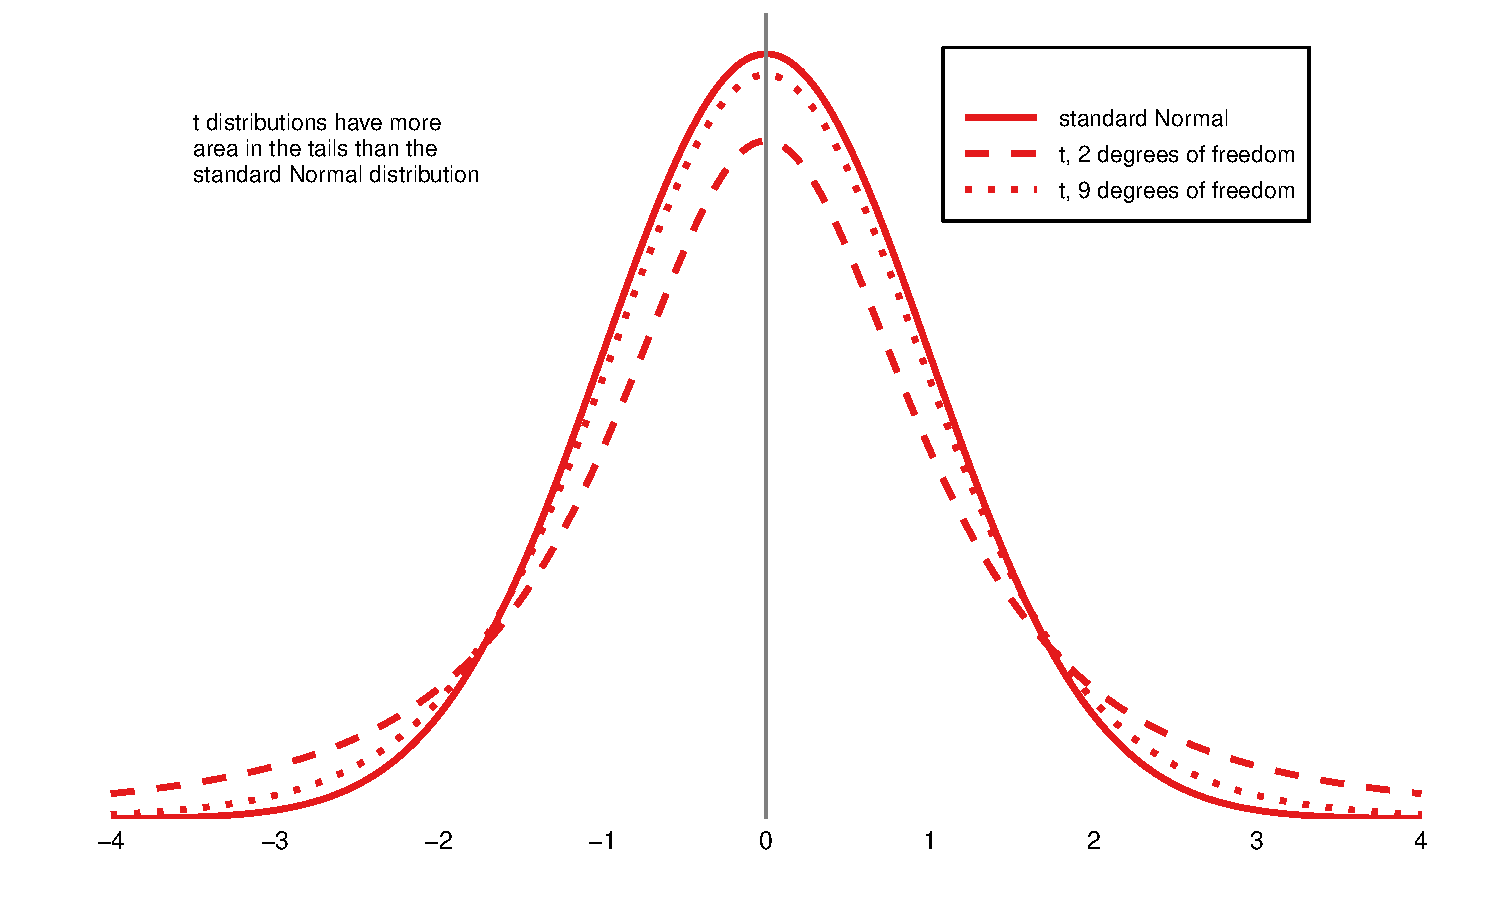
\includegraphics[keepaspectratio]{index_files/figure-pdf/fig-t-distributions-1.pdf}}

}

\caption{\label{fig-t-distributions}Comparison of t distributions with
different degrees of freedom to the standard Normal distribution}

\end{figure}%

\begin{Shaded}
\begin{Highlighting}[]
\CommentTok{\#| label: fig{-}critical{-}values{-}comparison}
\CommentTok{\#| fig{-}cap: "Comparison of 95\% critical values for standard Normal and t(5) distributions"}
\CommentTok{\#| fig{-}width: 11}
\CommentTok{\#| fig{-}height: 7}
\CommentTok{\#| warning: false}

\FunctionTok{library}\NormalTok{(ggplot2)}
\FunctionTok{library}\NormalTok{(gridExtra)}
\FunctionTok{library}\NormalTok{(grid)}

\CommentTok{\# Create x values}
\NormalTok{x }\OtherTok{\textless{}{-}} \FunctionTok{seq}\NormalTok{(}\SpecialCharTok{{-}}\DecValTok{4}\NormalTok{, }\DecValTok{4}\NormalTok{, }\AttributeTok{length.out =} \DecValTok{500}\NormalTok{)}

\CommentTok{\# Calculate densities}
\NormalTok{df\_plot }\OtherTok{\textless{}{-}} \FunctionTok{data.frame}\NormalTok{(}
  \AttributeTok{x =}\NormalTok{ x,}
  \AttributeTok{t\_density =} \FunctionTok{dt}\NormalTok{(x, }\AttributeTok{df =} \DecValTok{5}\NormalTok{),}
  \AttributeTok{normal\_density =} \FunctionTok{dnorm}\NormalTok{(x)}
\NormalTok{)}

\CommentTok{\# Critical values}
\NormalTok{t\_crit }\OtherTok{\textless{}{-}} \FunctionTok{qt}\NormalTok{(}\FloatTok{0.975}\NormalTok{, }\AttributeTok{df =} \DecValTok{5}\NormalTok{)  }\CommentTok{\# 2.571}
\NormalTok{z\_crit }\OtherTok{\textless{}{-}} \FunctionTok{qnorm}\NormalTok{(}\FloatTok{0.975}\NormalTok{)        }\CommentTok{\# 1.960}

\CommentTok{\# Create the plot}
\NormalTok{p }\OtherTok{\textless{}{-}} \FunctionTok{ggplot}\NormalTok{(df\_plot, }\FunctionTok{aes}\NormalTok{(}\AttributeTok{x =}\NormalTok{ x)) }\SpecialCharTok{+}
  \CommentTok{\# t distribution}
  \FunctionTok{geom\_line}\NormalTok{(}\FunctionTok{aes}\NormalTok{(}\AttributeTok{y =}\NormalTok{ t\_density), }\AttributeTok{color =} \StringTok{"black"}\NormalTok{, }\AttributeTok{linewidth =}\NormalTok{ .}\DecValTok{9}\NormalTok{) }\SpecialCharTok{+}
  \CommentTok{\# Normal distribution}
  \FunctionTok{geom\_line}\NormalTok{(}\FunctionTok{aes}\NormalTok{(}\AttributeTok{y =}\NormalTok{ normal\_density), }\AttributeTok{color =} \StringTok{"red"}\NormalTok{, }\AttributeTok{linewidth =}\NormalTok{ .}\DecValTok{9}\NormalTok{, }\AttributeTok{linetype =} \StringTok{"dashed"}\NormalTok{) }\SpecialCharTok{+}
  
  \CommentTok{\# Vertical lines at critical values}
  \FunctionTok{geom\_vline}\NormalTok{(}\AttributeTok{xintercept =} \FunctionTok{c}\NormalTok{(}\SpecialCharTok{{-}}\NormalTok{t\_crit, t\_crit), }
             \AttributeTok{color =} \StringTok{"black"}\NormalTok{, }\AttributeTok{linewidth =} \FloatTok{0.5}\NormalTok{, }\AttributeTok{linetype =} \StringTok{"solid"}\NormalTok{) }\SpecialCharTok{+}
  \FunctionTok{geom\_vline}\NormalTok{(}\AttributeTok{xintercept =} \FunctionTok{c}\NormalTok{(}\SpecialCharTok{{-}}\NormalTok{z\_crit, z\_crit), }
             \AttributeTok{color =} \StringTok{"red"}\NormalTok{, }\AttributeTok{linewidth =} \FloatTok{0.5}\NormalTok{, }\AttributeTok{linetype =} \StringTok{"dashed"}\NormalTok{) }\SpecialCharTok{+}
  
  \CommentTok{\# Mark and label critical values on x{-}axis}
  \FunctionTok{annotate}\NormalTok{(}\StringTok{"point"}\NormalTok{, }\AttributeTok{x =} \SpecialCharTok{{-}}\NormalTok{t\_crit, }\AttributeTok{y =} \DecValTok{0}\NormalTok{, }\AttributeTok{size =} \DecValTok{3}\NormalTok{, }\AttributeTok{color =} \StringTok{"black"}\NormalTok{) }\SpecialCharTok{+}
  \FunctionTok{annotate}\NormalTok{(}\StringTok{"point"}\NormalTok{, }\AttributeTok{x =}\NormalTok{ t\_crit, }\AttributeTok{y =} \DecValTok{0}\NormalTok{, }\AttributeTok{size =} \DecValTok{3}\NormalTok{, }\AttributeTok{color =} \StringTok{"black"}\NormalTok{) }\SpecialCharTok{+}
  \FunctionTok{annotate}\NormalTok{(}\StringTok{"text"}\NormalTok{, }\AttributeTok{x =} \SpecialCharTok{{-}}\NormalTok{t\_crit, }\AttributeTok{y =} \SpecialCharTok{{-}}\FloatTok{0.02}\NormalTok{, }\AttributeTok{label =} \StringTok{"({-}2.571)"}\NormalTok{, }
           \AttributeTok{size =} \FloatTok{3.5}\NormalTok{, }\AttributeTok{hjust =} \FloatTok{0.5}\NormalTok{) }\SpecialCharTok{+}
  \FunctionTok{annotate}\NormalTok{(}\StringTok{"text"}\NormalTok{, }\AttributeTok{x =}\NormalTok{ t\_crit, }\AttributeTok{y =} \SpecialCharTok{{-}}\FloatTok{0.02}\NormalTok{, }\AttributeTok{label =} \StringTok{"(2.571)"}\NormalTok{, }
           \AttributeTok{size =} \FloatTok{3.5}\NormalTok{, }\AttributeTok{hjust =} \FloatTok{0.5}\NormalTok{) }\SpecialCharTok{+}
  
  \CommentTok{\# Legend}
  \FunctionTok{annotate}\NormalTok{(}\StringTok{"segment"}\NormalTok{, }\AttributeTok{x =} \FloatTok{2.8}\NormalTok{, }\AttributeTok{xend =} \FloatTok{3.3}\NormalTok{, }\AttributeTok{y =} \FloatTok{0.35}\NormalTok{, }\AttributeTok{yend =} \FloatTok{0.35}\NormalTok{,}
           \AttributeTok{linewidth =} \FloatTok{1.3}\NormalTok{, }\AttributeTok{color =} \StringTok{"black"}\NormalTok{) }\SpecialCharTok{+}
  \FunctionTok{annotate}\NormalTok{(}\StringTok{"text"}\NormalTok{, }\AttributeTok{x =} \FloatTok{3.4}\NormalTok{, }\AttributeTok{y =} \FloatTok{0.35}\NormalTok{, }\AttributeTok{label =} \StringTok{"t(5)"}\NormalTok{, }\AttributeTok{hjust =} \DecValTok{0}\NormalTok{, }\AttributeTok{size =} \DecValTok{4}\NormalTok{) }\SpecialCharTok{+}
  
  \FunctionTok{annotate}\NormalTok{(}\StringTok{"segment"}\NormalTok{, }\AttributeTok{x =} \FloatTok{2.8}\NormalTok{, }\AttributeTok{xend =} \FloatTok{3.3}\NormalTok{, }\AttributeTok{y =} \FloatTok{0.32}\NormalTok{, }\AttributeTok{yend =} \FloatTok{0.32}\NormalTok{,}
           \AttributeTok{linewidth =} \FloatTok{1.3}\NormalTok{, }\AttributeTok{color =} \StringTok{"red"}\NormalTok{, }\AttributeTok{linetype =} \StringTok{"dashed"}\NormalTok{) }\SpecialCharTok{+}
  \FunctionTok{annotate}\NormalTok{(}\StringTok{"text"}\NormalTok{, }\AttributeTok{x =} \FloatTok{3.4}\NormalTok{, }\AttributeTok{y =} \FloatTok{0.32}\NormalTok{, }\AttributeTok{label =} \StringTok{"Normal"}\NormalTok{, }\AttributeTok{hjust =} \DecValTok{0}\NormalTok{, }\AttributeTok{size =} \DecValTok{4}\NormalTok{, }\AttributeTok{color =} \StringTok{"red"}\NormalTok{) }\SpecialCharTok{+}
  
  \CommentTok{\# Axes and theme}
  \FunctionTok{scale\_x\_continuous}\NormalTok{(}\AttributeTok{breaks =} \FunctionTok{seq}\NormalTok{(}\SpecialCharTok{{-}}\DecValTok{4}\NormalTok{, }\DecValTok{4}\NormalTok{, }\AttributeTok{by =} \DecValTok{2}\NormalTok{), }\AttributeTok{limits =} \FunctionTok{c}\NormalTok{(}\SpecialCharTok{{-}}\DecValTok{4}\NormalTok{, }\DecValTok{4}\NormalTok{)) }\SpecialCharTok{+}
  \FunctionTok{scale\_y\_continuous}\NormalTok{(}\AttributeTok{limits =} \FunctionTok{c}\NormalTok{(}\SpecialCharTok{{-}}\FloatTok{0.03}\NormalTok{, }\FloatTok{0.4}\NormalTok{), }\AttributeTok{expand =} \FunctionTok{c}\NormalTok{(}\DecValTok{0}\NormalTok{, }\DecValTok{0}\NormalTok{)) }\SpecialCharTok{+}
  \FunctionTok{labs}\NormalTok{(}
    \AttributeTok{title =} \StringTok{"C = 95\% critical values of z and t(5)"}\NormalTok{,}
    \AttributeTok{x =} \StringTok{"t"}\NormalTok{,}
    \AttributeTok{y =} \StringTok{"density"}
\NormalTok{  ) }\SpecialCharTok{+}
  \FunctionTok{theme\_minimal}\NormalTok{(}\AttributeTok{base\_size =} \DecValTok{13}\NormalTok{) }\SpecialCharTok{+}
  \FunctionTok{theme}\NormalTok{(}
    \AttributeTok{plot.title =} \FunctionTok{element\_text}\NormalTok{(}\AttributeTok{size =} \DecValTok{16}\NormalTok{, }\AttributeTok{face =} \StringTok{"bold"}\NormalTok{, }\AttributeTok{color =} \StringTok{"\#4472C4"}\NormalTok{, }\AttributeTok{hjust =} \FloatTok{0.5}\NormalTok{),}
    \AttributeTok{axis.title.x =} \FunctionTok{element\_text}\NormalTok{(}\AttributeTok{size =} \DecValTok{12}\NormalTok{),}
    \AttributeTok{axis.title.y =} \FunctionTok{element\_text}\NormalTok{(}\AttributeTok{size =} \DecValTok{12}\NormalTok{, }\AttributeTok{angle =} \DecValTok{90}\NormalTok{),}
    \AttributeTok{axis.text.x =} \FunctionTok{element\_text}\NormalTok{(}\AttributeTok{size =} \DecValTok{11}\NormalTok{, }\AttributeTok{color =} \StringTok{"black"}\NormalTok{),}
    \AttributeTok{axis.text.y =} \FunctionTok{element\_text}\NormalTok{(}\AttributeTok{size =} \DecValTok{11}\NormalTok{, }\AttributeTok{color =} \StringTok{"black"}\NormalTok{),}
    \AttributeTok{panel.grid.minor =} \FunctionTok{element\_blank}\NormalTok{(),}
    \AttributeTok{panel.background =} \FunctionTok{element\_rect}\NormalTok{(}\AttributeTok{fill =} \StringTok{"white"}\NormalTok{, }\AttributeTok{color =} \ConstantTok{NA}\NormalTok{),}
    \AttributeTok{plot.background =} \FunctionTok{element\_rect}\NormalTok{(}\AttributeTok{fill =} \StringTok{"white"}\NormalTok{, }\AttributeTok{color =} \ConstantTok{NA}\NormalTok{)}
\NormalTok{  )}

\CommentTok{\# Create the table}
\NormalTok{table\_data }\OtherTok{\textless{}{-}} \FunctionTok{data.frame}\NormalTok{(}
  \AttributeTok{df =} \FunctionTok{c}\NormalTok{(}\StringTok{"1"}\NormalTok{, }\StringTok{"..."}\NormalTok{, }\StringTok{"5"}\NormalTok{, }\StringTok{"..."}\NormalTok{, }\StringTok{"1000"}\NormalTok{, }\StringTok{"z*"}\NormalTok{),}
  \AttributeTok{c50 =} \FunctionTok{c}\NormalTok{(}\StringTok{"1.000"}\NormalTok{, }\StringTok{""}\NormalTok{, }\StringTok{"0.727"}\NormalTok{, }\StringTok{""}\NormalTok{, }\StringTok{"0.675"}\NormalTok{, }\StringTok{"0.674"}\NormalTok{),}
  \AttributeTok{c60 =} \FunctionTok{c}\NormalTok{(}\StringTok{"1.376"}\NormalTok{, }\StringTok{""}\NormalTok{, }\StringTok{"0.920"}\NormalTok{, }\StringTok{""}\NormalTok{, }\StringTok{"0.842"}\NormalTok{, }\StringTok{"0.842"}\NormalTok{),}
  \AttributeTok{c70 =} \FunctionTok{c}\NormalTok{(}\StringTok{"1.963"}\NormalTok{, }\StringTok{""}\NormalTok{, }\StringTok{"1.156"}\NormalTok{, }\StringTok{""}\NormalTok{, }\StringTok{"1.037"}\NormalTok{, }\StringTok{"1.036"}\NormalTok{),}
  \AttributeTok{c80 =} \FunctionTok{c}\NormalTok{(}\StringTok{"3.078"}\NormalTok{, }\StringTok{""}\NormalTok{, }\StringTok{"1.476"}\NormalTok{, }\StringTok{""}\NormalTok{, }\StringTok{"1.282"}\NormalTok{, }\StringTok{"1.282"}\NormalTok{),}
  \AttributeTok{c90 =} \FunctionTok{c}\NormalTok{(}\StringTok{"6.314"}\NormalTok{, }\StringTok{""}\NormalTok{, }\StringTok{"2.015"}\NormalTok{, }\StringTok{""}\NormalTok{, }\StringTok{"1.646"}\NormalTok{, }\StringTok{"1.645"}\NormalTok{),}
  \AttributeTok{c95 =} \FunctionTok{c}\NormalTok{(}\StringTok{"12.71"}\NormalTok{, }\StringTok{"..."}\NormalTok{, }\StringTok{"2.571"}\NormalTok{, }\StringTok{"..."}\NormalTok{, }\StringTok{"1.962"}\NormalTok{, }\StringTok{"1.960"}\NormalTok{),}
  \AttributeTok{c96 =} \FunctionTok{c}\NormalTok{(}\StringTok{"15.89"}\NormalTok{, }\StringTok{""}\NormalTok{, }\StringTok{"2.757"}\NormalTok{, }\StringTok{""}\NormalTok{, }\StringTok{"2.056"}\NormalTok{, }\StringTok{"2.054"}\NormalTok{),}
  \AttributeTok{c98 =} \FunctionTok{c}\NormalTok{(}\StringTok{"31.82"}\NormalTok{, }\StringTok{""}\NormalTok{, }\StringTok{"3.365"}\NormalTok{, }\StringTok{""}\NormalTok{, }\StringTok{"2.330"}\NormalTok{, }\StringTok{"2.326"}\NormalTok{),}
  \AttributeTok{c99 =} \FunctionTok{c}\NormalTok{(}\StringTok{"63.66"}\NormalTok{, }\StringTok{""}\NormalTok{, }\StringTok{"4.032"}\NormalTok{, }\StringTok{""}\NormalTok{, }\StringTok{"2.581"}\NormalTok{, }\StringTok{"2.576"}\NormalTok{),}
  \AttributeTok{c995 =} \FunctionTok{c}\NormalTok{(}\StringTok{"127.3"}\NormalTok{, }\StringTok{""}\NormalTok{, }\StringTok{"4.773"}\NormalTok{, }\StringTok{""}\NormalTok{, }\StringTok{"2.813"}\NormalTok{, }\StringTok{"2.807"}\NormalTok{),}
  \AttributeTok{c998 =} \FunctionTok{c}\NormalTok{(}\StringTok{"318.3"}\NormalTok{, }\StringTok{""}\NormalTok{, }\StringTok{"5.893"}\NormalTok{, }\StringTok{""}\NormalTok{, }\StringTok{"3.098"}\NormalTok{, }\StringTok{"3.090"}\NormalTok{),}
  \AttributeTok{c999 =} \FunctionTok{c}\NormalTok{(}\StringTok{"636.6"}\NormalTok{, }\StringTok{""}\NormalTok{, }\StringTok{"6.869"}\NormalTok{, }\StringTok{""}\NormalTok{, }\StringTok{"3.300"}\NormalTok{, }\StringTok{"3.291"}\NormalTok{)}
\NormalTok{)}

\CommentTok{\# Format table as grob}
\NormalTok{table\_grob }\OtherTok{\textless{}{-}} \FunctionTok{tableGrob}\NormalTok{(}
\NormalTok{  table\_data,}
  \AttributeTok{rows =} \ConstantTok{NULL}\NormalTok{,}
  \AttributeTok{cols =} \FunctionTok{c}\NormalTok{(}\StringTok{"Degrees of}\SpecialCharTok{\textbackslash{}n}\StringTok{Freedom"}\NormalTok{, }\StringTok{"50\%"}\NormalTok{, }\StringTok{"60\%"}\NormalTok{, }\StringTok{"70\%"}\NormalTok{, }\StringTok{"80\%"}\NormalTok{, }\StringTok{"90\%"}\NormalTok{, }
           \StringTok{"95\%"}\NormalTok{, }\StringTok{"96\%"}\NormalTok{, }\StringTok{"98\%"}\NormalTok{, }\StringTok{"99\%"}\NormalTok{, }\StringTok{"99.5\%"}\NormalTok{, }\StringTok{"99.8\%"}\NormalTok{, }\StringTok{"99.9\%"}\NormalTok{),}
  \AttributeTok{theme =} \FunctionTok{ttheme\_minimal}\NormalTok{(}
    \AttributeTok{core =} \FunctionTok{list}\NormalTok{(}
      \AttributeTok{fg\_params =} \FunctionTok{list}\NormalTok{(}\AttributeTok{hjust =} \FloatTok{0.5}\NormalTok{, }\AttributeTok{x =} \FloatTok{0.5}\NormalTok{, }\AttributeTok{fontsize =} \DecValTok{9}\NormalTok{),}
      \AttributeTok{bg\_params =} \FunctionTok{list}\NormalTok{(}\AttributeTok{fill =} \FunctionTok{c}\NormalTok{(}\StringTok{"white"}\NormalTok{, }\StringTok{"gray95"}\NormalTok{))}
\NormalTok{    ),}
    \AttributeTok{colhead =} \FunctionTok{list}\NormalTok{(}
      \AttributeTok{fg\_params =} \FunctionTok{list}\NormalTok{(}\AttributeTok{fontsize =} \DecValTok{9}\NormalTok{, }\AttributeTok{fontface =} \StringTok{"bold"}\NormalTok{),}
      \AttributeTok{bg\_params =} \FunctionTok{list}\NormalTok{(}\AttributeTok{fill =} \StringTok{"gray90"}\NormalTok{)}
\NormalTok{    )}
\NormalTok{  )}
\NormalTok{)}

\CommentTok{\# Add title to table}
\NormalTok{table\_title }\OtherTok{\textless{}{-}} \FunctionTok{textGrob}\NormalTok{(}\StringTok{"Confidence Level C"}\NormalTok{, }
                       \AttributeTok{gp =} \FunctionTok{gpar}\NormalTok{(}\AttributeTok{fontsize =} \DecValTok{10}\NormalTok{, }\AttributeTok{fontface =} \StringTok{"bold"}\NormalTok{))}

\CommentTok{\# Combine plot and table}
\FunctionTok{grid.arrange}\NormalTok{(}
\NormalTok{  p,}
  \FunctionTok{arrangeGrob}\NormalTok{(table\_title, table\_grob, }\AttributeTok{heights =} \FunctionTok{c}\NormalTok{(}\FloatTok{0.1}\NormalTok{, }\FloatTok{0.9}\NormalTok{)),}
  \AttributeTok{nrow =} \DecValTok{2}\NormalTok{,}
  \AttributeTok{heights =} \FunctionTok{c}\NormalTok{(}\FloatTok{0.6}\NormalTok{, }\FloatTok{0.4}\NormalTok{)}
\NormalTok{)}
\end{Highlighting}
\end{Shaded}

\pandocbounded{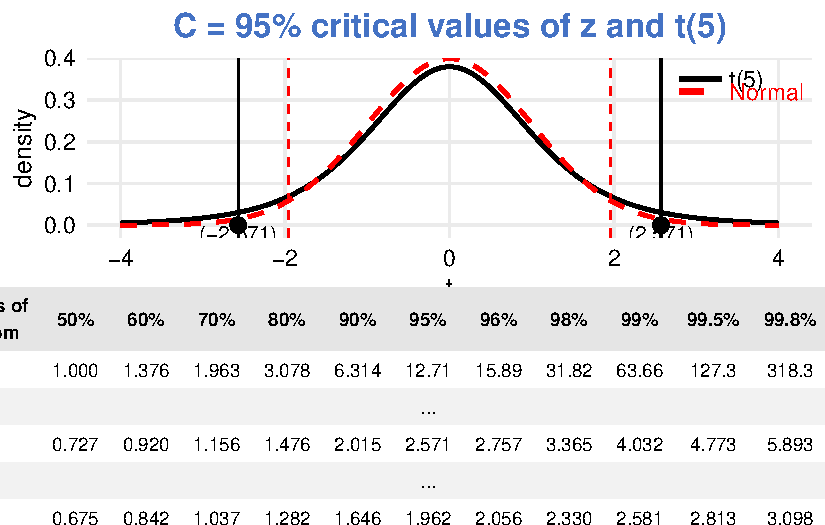
\includegraphics[keepaspectratio]{index_files/figure-pdf/unnamed-chunk-51-1.pdf}}

\section{Understanding Null Hypothesis Significance
Testing}\label{understanding-null-hypothesis-significance-testing}

You've likely encountered statements like these in academic publications
and research papers:

``The finding achieved statistical significance, \(p < .05\).''

``We rejected the null hypothesis indicating no difference and
determined there was a statistically significant increase at the .01
level.''

These statements represent \emph{null hypothesis significance testing}
(NHST), the conventional framework for statistical inference across
numerous fields. Understanding NHST---particularly \(p\) values---is
essential for interpreting research that employs these methods. The good
news is that NHST shares strong conceptual and mathematical connections
with confidence interval estimation, including similar statistical
formulas. As we explore NHST, draw on your knowledge of CIs to help make
sense of these concepts.

This chapter covers the following topics:

\begin{itemize}
\tightlist
\item
  The fundamentals of NHST and \(p\) values
\item
  \(p\) values and the normal distribution
\item
  \(p\) values and the \(t\) distribution
\item
  Converting between CIs and \(p\) values (in both directions)
\item
  Four critical warnings about NHST and \(p\) values: The four red flags
\item
  NHST decision-making: The alternative hypothesis, and Type I and Type
  II errors
\end{itemize}

\section{\texorpdfstring{The Fundamentals of NHST and \(p\)
Values}{The Fundamentals of NHST and p Values}}\label{the-fundamentals-of-nhst-and-p-values}

The approach we refer to as NHST actually combines two distinct
methodological frameworks: one pioneered by Sir Ronald Fisher, and
another developed by Jerzy Neyman and Egon Pearson, who notably held
opposing views to Fisher's. While Salsburg (2001) provides engaging
accounts of these historical debates and the early development of
statistical methods, we'll focus on the integrated approach that
researchers predominantly employ today.

Let's revisit the polling example from Chapter 1, where we estimated
support for Proposition A at 53\% {[}51, 55{]}. Figure 6.1 displays this
result, with the cat's eye indicating the 95\% CI. Remember that the CI
and its accompanying cat's eye convey that values near 53\% represent
the most credible estimates for the true level of support. Values
approaching or exceeding the interval limits become progressively less
credible, while values substantially beyond the CI---such as 50\% or
56\%---are comparatively implausible, though not entirely impossible. As
always, keep in mind the possibility that our CI could be red.

Now let's examine NHST and \(p\) values. The procedure involves three
steps:

\begin{enumerate}
\def\labelenumi{\arabic{enumi}.}
\item
  \textbf{Formulate a null hypothesis.} The null hypothesis represents a
  claim about the population parameter that we aim to evaluate. It
  designates a single reference value that serves as our baseline for
  testing. In this polling scenario, we would likely specify 50\% as our
  null hypothesis value, yielding the statement: ``support for the
  proposition stands at 50\% in the population''---the threshold
  required for passage. Null hypotheses frequently assert that no change
  has occurred or that an effect equals zero.
\item
  \textbf{Compute the \(p\) value.} Using the observed data, we
  calculate the \(p\) value, which informally quantifies how improbable
  results similar to ours would be IF the null hypothesis were true. The
  ``IF'' clause is crucial: calculating a \(p\) value requires assuming
  the null hypothesis holds. Consequently, a \(p\) value reflects both
  our data and our specified null hypothesis. For our polling data, with
  a null hypothesis of 50\% population support, the \(p\) value equals
  .003. This indicates that obtaining poll results like ours would be
  highly improbable IF the population truly had 50\% support. We
  therefore have reasonable grounds to question that null hypothesis.
  More broadly, a small \(p\) value casts doubt on the null hypothesis.
\item
  \textbf{Determine whether to reject the null hypothesis.} NHST
  compares the obtained \(p\) value against a criterion termed the
  \emph{significance level}, commonly set at .05. When \(p\) falls below
  this threshold, we doubt the null hypothesis sufficiently to reject
  it, declaring we have detected a \emph{statistically significant
  effect}. When \(p\) exceeds the significance level, we fail to reject
  the null hypothesis, stating we have a \emph{statistically
  nonsignificant effect} or that we did not achieve statistical
  significance. Note the precise language: we say the null hypothesis is
  ``not rejected'' rather than ``accepted.'' These double negatives are
  an inherent feature of NHST terminology.
\end{enumerate}

The significance level---frequently .05---establishes the criterion for
null hypothesis rejection. Formally, researchers should specify this
level before examining the data; we might call this \emph{strict NHST}.
In practice, however, most researchers do not pre-specify their intended
significance level. Instead, they compare the obtained \(p\) value
against several conventional significance levels: typically .05, .01,
and .001, as illustrated in Figure 6.2. For instance, obtaining
\(p = .017\) justifies rejecting the null hypothesis at the .05 level,
while \(p = .006\) permits rejection at the .01 level. Researchers
report the smallest significance level that allows rejection, since
rejecting at a more stringent level (.01 versus .05) provides stronger
evidence. The researcher thus tailors their conclusion based on where
\(p\) falls relative to these conventional thresholds, and might
conclude:

\begin{Shaded}
\begin{Highlighting}[]
\FunctionTok{library}\NormalTok{(ggplot2)}

\CommentTok{\# Create data for the three significance level markers}
\NormalTok{sig\_levels }\OtherTok{\textless{}{-}} \FunctionTok{data.frame}\NormalTok{(}
  \AttributeTok{x =} \FunctionTok{c}\NormalTok{(}\FloatTok{0.001}\NormalTok{, }\FloatTok{0.01}\NormalTok{, }\FloatTok{0.05}\NormalTok{),}
  \AttributeTok{y =} \FunctionTok{c}\NormalTok{(}\FloatTok{2.8}\NormalTok{, }\FloatTok{1.8}\NormalTok{, }\FloatTok{0.9}\NormalTok{),}
  \AttributeTok{box\_width =} \FunctionTok{c}\NormalTok{(}\FloatTok{0.025}\NormalTok{, }\FloatTok{0.02}\NormalTok{, }\FloatTok{0.018}\NormalTok{),}
  \AttributeTok{box\_height =} \FunctionTok{c}\NormalTok{(}\FloatTok{0.6}\NormalTok{, }\FloatTok{0.5}\NormalTok{, }\FloatTok{0.45}\NormalTok{),}
  \AttributeTok{label =} \FunctionTok{c}\NormalTok{(}\StringTok{".001"}\NormalTok{, }\StringTok{".01"}\NormalTok{, }\StringTok{".05"}\NormalTok{)}
\NormalTok{)}

\CommentTok{\# Create the plot}
\FunctionTok{ggplot}\NormalTok{() }\SpecialCharTok{+}
  \CommentTok{\# Add vertical line at origin}
  \FunctionTok{geom\_segment}\NormalTok{(}\FunctionTok{aes}\NormalTok{(}\AttributeTok{x =} \DecValTok{0}\NormalTok{, }\AttributeTok{y =} \DecValTok{0}\NormalTok{, }\AttributeTok{xend =} \DecValTok{0}\NormalTok{, }\AttributeTok{yend =} \FloatTok{3.2}\NormalTok{),}
               \AttributeTok{linewidth =} \DecValTok{1}\NormalTok{, }\AttributeTok{color =} \StringTok{"black"}\NormalTok{) }\SpecialCharTok{+}
  
  \CommentTok{\# Add horizontal axis line}
  \FunctionTok{geom\_segment}\NormalTok{(}\FunctionTok{aes}\NormalTok{(}\AttributeTok{x =} \DecValTok{0}\NormalTok{, }\AttributeTok{y =} \DecValTok{0}\NormalTok{, }\AttributeTok{xend =} \FloatTok{0.22}\NormalTok{, }\AttributeTok{yend =} \DecValTok{0}\NormalTok{),}
               \AttributeTok{linewidth =} \DecValTok{1}\NormalTok{, }\AttributeTok{color =} \StringTok{"black"}\NormalTok{) }\SpecialCharTok{+}
  
  \CommentTok{\# Add tick marks on x{-}axis}
  \FunctionTok{geom\_segment}\NormalTok{(}\FunctionTok{aes}\NormalTok{(}\AttributeTok{x =} \FunctionTok{c}\NormalTok{(}\DecValTok{0}\NormalTok{, }\FloatTok{0.1}\NormalTok{, }\FloatTok{0.2}\NormalTok{), }\AttributeTok{xend =} \FunctionTok{c}\NormalTok{(}\DecValTok{0}\NormalTok{, }\FloatTok{0.1}\NormalTok{, }\FloatTok{0.2}\NormalTok{),}
                   \AttributeTok{y =} \DecValTok{0}\NormalTok{, }\AttributeTok{yend =} \SpecialCharTok{{-}}\FloatTok{0.15}\NormalTok{),}
               \AttributeTok{linewidth =} \DecValTok{1}\NormalTok{) }\SpecialCharTok{+}
  
  \CommentTok{\# Add diagonal lines from axis to boxes}
  \FunctionTok{geom\_segment}\NormalTok{(}\AttributeTok{data =}\NormalTok{ sig\_levels,}
               \FunctionTok{aes}\NormalTok{(}\AttributeTok{x =}\NormalTok{ x, }\AttributeTok{y =} \DecValTok{0}\NormalTok{, }\AttributeTok{xend =}\NormalTok{ x, }\AttributeTok{yend =}\NormalTok{ y }\SpecialCharTok{{-}}\NormalTok{ box\_height}\SpecialCharTok{/}\DecValTok{2} \SpecialCharTok{{-}} \FloatTok{0.05}\NormalTok{),}
               \AttributeTok{linewidth =} \DecValTok{1}\NormalTok{, }\AttributeTok{color =} \StringTok{"black"}\NormalTok{) }\SpecialCharTok{+}
  
  \CommentTok{\# Add speech bubble style boxes}
  \FunctionTok{geom\_rect}\NormalTok{(}\AttributeTok{data =}\NormalTok{ sig\_levels,}
            \FunctionTok{aes}\NormalTok{(}\AttributeTok{xmin =}\NormalTok{ x }\SpecialCharTok{{-}}\NormalTok{ box\_width, }\AttributeTok{xmax =}\NormalTok{ x }\SpecialCharTok{+}\NormalTok{ box\_width,}
                \AttributeTok{ymin =}\NormalTok{ y }\SpecialCharTok{{-}}\NormalTok{ box\_height}\SpecialCharTok{/}\DecValTok{2}\NormalTok{, }\AttributeTok{ymax =}\NormalTok{ y }\SpecialCharTok{+}\NormalTok{ box\_height}\SpecialCharTok{/}\DecValTok{2}\NormalTok{),}
            \AttributeTok{fill =} \StringTok{"paleturquoise1"}\NormalTok{, }\AttributeTok{color =} \StringTok{"black"}\NormalTok{, }\AttributeTok{linewidth =} \FloatTok{1.5}\NormalTok{) }\SpecialCharTok{+}
  
  \CommentTok{\# Add small triangle/tail for speech bubble effect}
  \FunctionTok{geom\_polygon}\NormalTok{(}\AttributeTok{data =} \FunctionTok{data.frame}\NormalTok{(}
    \AttributeTok{x =} \FunctionTok{c}\NormalTok{(}\FloatTok{0.001} \SpecialCharTok{{-}} \FloatTok{0.003}\NormalTok{, }\FloatTok{0.001} \SpecialCharTok{+} \FloatTok{0.003}\NormalTok{, }\FloatTok{0.001}\NormalTok{,}
          \FloatTok{0.01} \SpecialCharTok{{-}} \FloatTok{0.003}\NormalTok{, }\FloatTok{0.01} \SpecialCharTok{+} \FloatTok{0.003}\NormalTok{, }\FloatTok{0.01}\NormalTok{,}
          \FloatTok{0.05} \SpecialCharTok{{-}} \FloatTok{0.003}\NormalTok{, }\FloatTok{0.05} \SpecialCharTok{+} \FloatTok{0.003}\NormalTok{, }\FloatTok{0.05}\NormalTok{),}
    \AttributeTok{y =} \FunctionTok{c}\NormalTok{(}\FunctionTok{rep}\NormalTok{(}\FunctionTok{c}\NormalTok{(sig\_levels}\SpecialCharTok{$}\NormalTok{y[}\DecValTok{1}\NormalTok{] }\SpecialCharTok{{-}}\NormalTok{ sig\_levels}\SpecialCharTok{$}\NormalTok{box\_height[}\DecValTok{1}\NormalTok{]}\SpecialCharTok{/}\DecValTok{2}\NormalTok{,}
\NormalTok{                sig\_levels}\SpecialCharTok{$}\NormalTok{y[}\DecValTok{1}\NormalTok{] }\SpecialCharTok{{-}}\NormalTok{ sig\_levels}\SpecialCharTok{$}\NormalTok{box\_height[}\DecValTok{1}\NormalTok{]}\SpecialCharTok{/}\DecValTok{2}\NormalTok{,}
\NormalTok{                sig\_levels}\SpecialCharTok{$}\NormalTok{y[}\DecValTok{1}\NormalTok{] }\SpecialCharTok{{-}}\NormalTok{ sig\_levels}\SpecialCharTok{$}\NormalTok{box\_height[}\DecValTok{1}\NormalTok{]}\SpecialCharTok{/}\DecValTok{2} \SpecialCharTok{{-}} \FloatTok{0.15}\NormalTok{), }\DecValTok{1}\NormalTok{),}
          \FunctionTok{rep}\NormalTok{(}\FunctionTok{c}\NormalTok{(sig\_levels}\SpecialCharTok{$}\NormalTok{y[}\DecValTok{2}\NormalTok{] }\SpecialCharTok{{-}}\NormalTok{ sig\_levels}\SpecialCharTok{$}\NormalTok{box\_height[}\DecValTok{2}\NormalTok{]}\SpecialCharTok{/}\DecValTok{2}\NormalTok{,}
\NormalTok{                sig\_levels}\SpecialCharTok{$}\NormalTok{y[}\DecValTok{2}\NormalTok{] }\SpecialCharTok{{-}}\NormalTok{ sig\_levels}\SpecialCharTok{$}\NormalTok{box\_height[}\DecValTok{2}\NormalTok{]}\SpecialCharTok{/}\DecValTok{2}\NormalTok{,}
\NormalTok{                sig\_levels}\SpecialCharTok{$}\NormalTok{y[}\DecValTok{2}\NormalTok{] }\SpecialCharTok{{-}}\NormalTok{ sig\_levels}\SpecialCharTok{$}\NormalTok{box\_height[}\DecValTok{2}\NormalTok{]}\SpecialCharTok{/}\DecValTok{2} \SpecialCharTok{{-}} \FloatTok{0.15}\NormalTok{), }\DecValTok{1}\NormalTok{),}
          \FunctionTok{rep}\NormalTok{(}\FunctionTok{c}\NormalTok{(sig\_levels}\SpecialCharTok{$}\NormalTok{y[}\DecValTok{3}\NormalTok{] }\SpecialCharTok{{-}}\NormalTok{ sig\_levels}\SpecialCharTok{$}\NormalTok{box\_height[}\DecValTok{3}\NormalTok{]}\SpecialCharTok{/}\DecValTok{2}\NormalTok{,}
\NormalTok{                sig\_levels}\SpecialCharTok{$}\NormalTok{y[}\DecValTok{3}\NormalTok{] }\SpecialCharTok{{-}}\NormalTok{ sig\_levels}\SpecialCharTok{$}\NormalTok{box\_height[}\DecValTok{3}\NormalTok{]}\SpecialCharTok{/}\DecValTok{2}\NormalTok{,}
\NormalTok{                sig\_levels}\SpecialCharTok{$}\NormalTok{y[}\DecValTok{3}\NormalTok{] }\SpecialCharTok{{-}}\NormalTok{ sig\_levels}\SpecialCharTok{$}\NormalTok{box\_height[}\DecValTok{3}\NormalTok{]}\SpecialCharTok{/}\DecValTok{2} \SpecialCharTok{{-}} \FloatTok{0.15}\NormalTok{), }\DecValTok{1}\NormalTok{)),}
    \AttributeTok{group =} \FunctionTok{rep}\NormalTok{(}\DecValTok{1}\SpecialCharTok{:}\DecValTok{3}\NormalTok{, }\AttributeTok{each =} \DecValTok{3}\NormalTok{)}
\NormalTok{  ), }\FunctionTok{aes}\NormalTok{(}\AttributeTok{x =}\NormalTok{ x, }\AttributeTok{y =}\NormalTok{ y, }\AttributeTok{group =}\NormalTok{ group),}
  \AttributeTok{fill =} \StringTok{"paleturquoise1"}\NormalTok{, }\AttributeTok{color =} \StringTok{"black"}\NormalTok{, }\AttributeTok{linewidth =} \FloatTok{1.5}\NormalTok{) }\SpecialCharTok{+}  \CommentTok{\# CHANGED: fill = "" to fill = "paleturquoise1"}
  
  \CommentTok{\# Add labels inside boxes}
  \FunctionTok{geom\_text}\NormalTok{(}\AttributeTok{data =}\NormalTok{ sig\_levels,}
            \FunctionTok{aes}\NormalTok{(}\AttributeTok{x =}\NormalTok{ x, }\AttributeTok{y =}\NormalTok{ y, }\AttributeTok{label =}\NormalTok{ label),}
            \AttributeTok{size =} \DecValTok{8}\NormalTok{, }\AttributeTok{fontface =} \StringTok{"bold"}\NormalTok{, }\AttributeTok{color =} \StringTok{"\#CC0000"}\NormalTok{) }\SpecialCharTok{+}
  
  \CommentTok{\# Add x{-}axis labels}
  \FunctionTok{annotate}\NormalTok{(}\StringTok{"text"}\NormalTok{, }\AttributeTok{x =} \FunctionTok{c}\NormalTok{(}\DecValTok{0}\NormalTok{, }\FloatTok{0.1}\NormalTok{, }\FloatTok{0.2}\NormalTok{), }\AttributeTok{y =} \SpecialCharTok{{-}}\FloatTok{0.35}\NormalTok{,}
           \AttributeTok{label =} \FunctionTok{c}\NormalTok{(}\StringTok{"0"}\NormalTok{, }\StringTok{".1"}\NormalTok{, }\StringTok{".2"}\NormalTok{),}
           \AttributeTok{size =} \DecValTok{8}\NormalTok{, }\AttributeTok{fontface =} \StringTok{"bold"}\NormalTok{, }\AttributeTok{color =} \StringTok{"\#CC0000"}\NormalTok{) }\SpecialCharTok{+}
  
  \CommentTok{\# Set plot limits and remove default elements}
  \FunctionTok{coord\_cartesian}\NormalTok{(}\AttributeTok{xlim =} \FunctionTok{c}\NormalTok{(}\SpecialCharTok{{-}}\FloatTok{0.01}\NormalTok{, }\FloatTok{0.23}\NormalTok{), }\AttributeTok{ylim =} \FunctionTok{c}\NormalTok{(}\SpecialCharTok{{-}}\FloatTok{0.5}\NormalTok{, }\FloatTok{3.4}\NormalTok{), }\AttributeTok{clip =} \StringTok{"off"}\NormalTok{) }\SpecialCharTok{+}
  \FunctionTok{theme\_void}\NormalTok{() }\SpecialCharTok{+} 
  \FunctionTok{theme}\NormalTok{(}\AttributeTok{plot.margin =} \FunctionTok{margin}\NormalTok{(}\DecValTok{20}\NormalTok{, }\DecValTok{20}\NormalTok{, }\DecValTok{20}\NormalTok{, }\DecValTok{20}\NormalTok{))}
\end{Highlighting}
\end{Shaded}

\begin{figure}[H]

\centering{

\pandocbounded{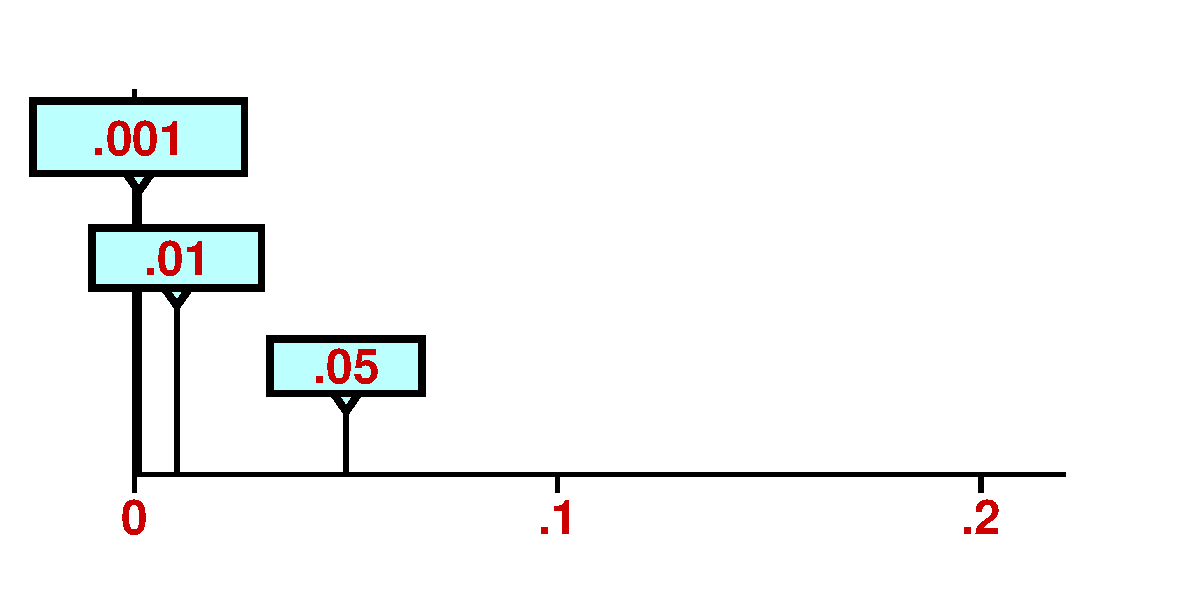
\includegraphics[keepaspectratio]{index_files/figure-pdf/fig-significance-levels-1.pdf}}

}

\caption{\label{fig-significance-levels}The three most commonly used
significance levels, .05, .01, and .001, shown on a scale representing
the possible range of \(p\) values from 0 to 1.}

\end{figure}%

The researcher may also make corresponding statements about statistical
significance, such as: ``The effect was statistically significant at the
.05 level.''

Or ``\ldots was statistically significant, p \textless{} .001.''

The threshold that determines whether researchers reject the null
hypothesis is known as the significance level. When a calculated p-value
falls below this threshold, the null hypothesis is rejected; when it
exceeds the threshold, the null hypothesis is retained. Lower
significance levels are generally favored in research because they yield
more persuasive conclusions. The rationale becomes clear when we
consider what a p-value represents: it quantifies how probable our
observed results would be assuming the null hypothesis holds true.
Consequently, diminishing p-values indicate increasingly improbable
outcomes under the null hypothesis framework. This improbability
strengthens our justification for questioning the null hypothesis,
thereby furnishing more compelling evidence for its rejection.

Adopting a more stringent significance level---such as .01 instead of
.05---necessitates obtaining a correspondingly smaller p-value. Thus,
more rigorous significance thresholds translate to more robust evidence
contradicting the null hypothesis and more persuasive grounds for its
rejection. Within the research community, p-values are typically
interpreted as metrics of evidential strength against the null
hypothesis: diminishing p-values correspond to mounting evidence, which
bolsters researchers' confidence when rejecting the null. This
perspective explains why researchers might articulate statements such as
``p \textless{} .001, indicating exceptionally strong evidence against
the null hypothesis.''

Best practices in null hypothesis significance testing require reporting
precise p-values---such as p = .30, p = .04, or p = .007---rather than
merely indicating whether they cross conventional thresholds (e.g., p
\textgreater{} .05, p \textless{} .05, p \textless{} .01). This approach
offers comprehensive information while permitting readers to evaluate
findings against whatever significance criterion they deem appropriate.

Traditionally, null hypothesis significance testing proceeds through
direct computation of p-values without invoking confidence intervals.
However, when confidence intervals are available, straightforward
methods exist for converting between estimation frameworks and p-value
interpretations. When working with the .05 significance threshold, the
fundamental correspondence between a 95\% confidence interval and its
associated p-value---depicted in Figure above---can be articulated in
the following manner:

\begin{Shaded}
\begin{Highlighting}[]
\CommentTok{\#| label: fig{-}ci{-}rejection{-}regions}
\CommentTok{\#| fig{-}cap: "CI with rejection (red) vs. non{-}rejection (blue) regions. If the null value falls outside the CI, reject; inside, do not reject."}
\CommentTok{\#| fig{-}width: 10}
\CommentTok{\#| fig{-}height: 6}

\FunctionTok{library}\NormalTok{(ggplot2)}
\FunctionTok{library}\NormalTok{(grid)  }\CommentTok{\# unit()}

\NormalTok{ci\_lower }\OtherTok{\textless{}{-}} \DecValTok{51}
\NormalTok{ci\_upper }\OtherTok{\textless{}{-}} \DecValTok{55}
\NormalTok{point\_estimate }\OtherTok{\textless{}{-}} \DecValTok{53}

\FunctionTok{ggplot}\NormalTok{() }\SpecialCharTok{+}
  \CommentTok{\# CI bar + dot}
  \FunctionTok{geom\_segment}\NormalTok{(}\FunctionTok{aes}\NormalTok{(}\AttributeTok{x =}\NormalTok{ ci\_lower, }\AttributeTok{xend =}\NormalTok{ ci\_upper, }\AttributeTok{y =} \FloatTok{1.2}\NormalTok{, }\AttributeTok{yend =} \FloatTok{1.2}\NormalTok{),}
               \AttributeTok{linewidth =} \DecValTok{2}\NormalTok{, }\AttributeTok{color =} \StringTok{"\#3366CC"}\NormalTok{) }\SpecialCharTok{+}
  \FunctionTok{geom\_point}\NormalTok{(}\FunctionTok{aes}\NormalTok{(}\AttributeTok{x =}\NormalTok{ point\_estimate, }\AttributeTok{y =} \FloatTok{1.2}\NormalTok{), }\AttributeTok{size =} \DecValTok{10}\NormalTok{, }\AttributeTok{color =} \StringTok{"\#19478A"}\NormalTok{) }\SpecialCharTok{+}

  \CommentTok{\# Brackets}
  \FunctionTok{geom\_segment}\NormalTok{(}\FunctionTok{aes}\NormalTok{(}\AttributeTok{x =}\NormalTok{ ci\_lower, }\AttributeTok{xend =}\NormalTok{ ci\_lower, }\AttributeTok{y =} \FloatTok{0.5}\NormalTok{, }\AttributeTok{yend =} \FloatTok{2.0}\NormalTok{), }\AttributeTok{linewidth =} \FloatTok{1.8}\NormalTok{) }\SpecialCharTok{+}
  \FunctionTok{geom\_segment}\NormalTok{(}\FunctionTok{aes}\NormalTok{(}\AttributeTok{x =}\NormalTok{ ci\_upper, }\AttributeTok{xend =}\NormalTok{ ci\_upper, }\AttributeTok{y =} \FloatTok{0.5}\NormalTok{, }\AttributeTok{yend =} \FloatTok{2.0}\NormalTok{), }\AttributeTok{linewidth =} \FloatTok{1.8}\NormalTok{) }\SpecialCharTok{+}

  \CommentTok{\# Double guide lines at top (note: y \& yend!)}
  \FunctionTok{geom\_segment}\NormalTok{(}\FunctionTok{aes}\NormalTok{(}\AttributeTok{x =} \FloatTok{49.5}\NormalTok{, }\AttributeTok{xend =} \FloatTok{56.5}\NormalTok{, }\AttributeTok{y =} \FloatTok{2.0}\NormalTok{,  }\AttributeTok{yend =} \FloatTok{2.0}\NormalTok{),  }\AttributeTok{linewidth =} \FloatTok{1.5}\NormalTok{) }\SpecialCharTok{+}
  \FunctionTok{geom\_segment}\NormalTok{(}\FunctionTok{aes}\NormalTok{(}\AttributeTok{x =} \FloatTok{49.5}\NormalTok{, }\AttributeTok{xend =} \FloatTok{56.5}\NormalTok{, }\AttributeTok{y =} \FloatTok{1.85}\NormalTok{, }\AttributeTok{yend =} \FloatTok{1.85}\NormalTok{), }\AttributeTok{linewidth =} \FloatTok{1.5}\NormalTok{) }\SpecialCharTok{+}

  \CommentTok{\# Bottom guide line}
  \FunctionTok{geom\_segment}\NormalTok{(}\FunctionTok{aes}\NormalTok{(}\AttributeTok{x =} \FloatTok{49.5}\NormalTok{, }\AttributeTok{xend =} \FloatTok{56.5}\NormalTok{, }\AttributeTok{y =} \FloatTok{0.5}\NormalTok{,  }\AttributeTok{yend =} \FloatTok{0.5}\NormalTok{),  }\AttributeTok{linewidth =} \FloatTok{1.5}\NormalTok{) }\SpecialCharTok{+}

  \CommentTok{\# Arrows}
  \FunctionTok{geom\_segment}\NormalTok{(}\FunctionTok{aes}\NormalTok{(}\AttributeTok{x =} \FloatTok{49.5}\NormalTok{, }\AttributeTok{xend =} \FloatTok{48.5}\NormalTok{, }\AttributeTok{y =} \FloatTok{1.2}\NormalTok{, }\AttributeTok{yend =} \FloatTok{1.2}\NormalTok{),}
               \AttributeTok{linewidth =} \FloatTok{1.8}\NormalTok{, }\AttributeTok{arrow =} \FunctionTok{arrow}\NormalTok{(}\AttributeTok{length =} \FunctionTok{unit}\NormalTok{(}\FloatTok{0.35}\NormalTok{, }\StringTok{"cm"}\NormalTok{), }\AttributeTok{type =} \StringTok{"closed"}\NormalTok{)) }\SpecialCharTok{+}
  \FunctionTok{geom\_segment}\NormalTok{(}\FunctionTok{aes}\NormalTok{(}\AttributeTok{x =} \FloatTok{56.5}\NormalTok{, }\AttributeTok{xend =} \FloatTok{57.5}\NormalTok{, }\AttributeTok{y =} \FloatTok{1.2}\NormalTok{, }\AttributeTok{yend =} \FloatTok{1.2}\NormalTok{),}
               \AttributeTok{linewidth =} \FloatTok{1.8}\NormalTok{, }\AttributeTok{arrow =} \FunctionTok{arrow}\NormalTok{(}\AttributeTok{length =} \FunctionTok{unit}\NormalTok{(}\FloatTok{0.35}\NormalTok{, }\StringTok{"cm"}\NormalTok{), }\AttributeTok{type =} \StringTok{"closed"}\NormalTok{)) }\SpecialCharTok{+}

  \CommentTok{\# Text (staggered y to avoid overlap)}
  \FunctionTok{annotate}\NormalTok{(}\StringTok{"text"}\NormalTok{, }\AttributeTok{x =} \FloatTok{50.25}\NormalTok{, }\AttributeTok{y =} \FloatTok{4.1}\NormalTok{,}
           \AttributeTok{label =} \StringTok{"If the null hypothesis}\SpecialCharTok{\textbackslash{}n}\StringTok{value is anywhere}\SpecialCharTok{\textbackslash{}n}\StringTok{here, reject"}\NormalTok{,}
           \AttributeTok{color =} \StringTok{"\#CC0000"}\NormalTok{, }\AttributeTok{size =} \FloatTok{4.2}\NormalTok{, }\AttributeTok{fontface =} \StringTok{"bold"}\NormalTok{, }\AttributeTok{lineheight =} \FloatTok{0.9}\NormalTok{) }\SpecialCharTok{+}
  \FunctionTok{annotate}\NormalTok{(}\StringTok{"text"}\NormalTok{, }\AttributeTok{x =} \FloatTok{53.00}\NormalTok{, }\AttributeTok{y =} \FloatTok{3.3}\NormalTok{,}
           \AttributeTok{label =} \StringTok{"If the null hypothesis value is anywhere here, don\textquotesingle{}t reject"}\NormalTok{,}
           \AttributeTok{color =} \StringTok{"\#4D4D4D"}\NormalTok{, }\AttributeTok{size =} \FloatTok{4.0}\NormalTok{, }\AttributeTok{lineheight =} \FloatTok{0.9}\NormalTok{) }\SpecialCharTok{+}
  \FunctionTok{annotate}\NormalTok{(}\StringTok{"text"}\NormalTok{, }\AttributeTok{x =} \FloatTok{55.75}\NormalTok{, }\AttributeTok{y =} \FloatTok{4.1}\NormalTok{,}
           \AttributeTok{label =} \StringTok{"If the null hypothesis}\SpecialCharTok{\textbackslash{}n}\StringTok{value is anywhere}\SpecialCharTok{\textbackslash{}n}\StringTok{here, reject"}\NormalTok{,}
           \AttributeTok{color =} \StringTok{"\#CC0000"}\NormalTok{, }\AttributeTok{size =} \FloatTok{4.2}\NormalTok{, }\AttributeTok{fontface =} \StringTok{"bold"}\NormalTok{, }\AttributeTok{lineheight =} \FloatTok{0.9}\NormalTok{) }\SpecialCharTok{+}

  \CommentTok{\# Axis baseline + ticks + labels}
  \FunctionTok{geom\_segment}\NormalTok{(}\FunctionTok{aes}\NormalTok{(}\AttributeTok{x =} \DecValTok{50}\NormalTok{, }\AttributeTok{xend =} \DecValTok{56}\NormalTok{, }\AttributeTok{y =} \SpecialCharTok{{-}}\FloatTok{0.3}\NormalTok{, }\AttributeTok{yend =} \SpecialCharTok{{-}}\FloatTok{0.3}\NormalTok{), }\AttributeTok{linewidth =} \DecValTok{1}\NormalTok{) }\SpecialCharTok{+}
  \FunctionTok{geom\_segment}\NormalTok{(}\FunctionTok{aes}\NormalTok{(}\AttributeTok{x =} \FunctionTok{seq}\NormalTok{(}\DecValTok{50}\NormalTok{, }\DecValTok{56}\NormalTok{, }\DecValTok{1}\NormalTok{), }\AttributeTok{xend =} \FunctionTok{seq}\NormalTok{(}\DecValTok{50}\NormalTok{, }\DecValTok{56}\NormalTok{, }\DecValTok{1}\NormalTok{), }\AttributeTok{y =} \SpecialCharTok{{-}}\FloatTok{0.3}\NormalTok{, }\AttributeTok{yend =} \SpecialCharTok{{-}}\FloatTok{0.42}\NormalTok{),}
               \AttributeTok{linewidth =} \DecValTok{1}\NormalTok{) }\SpecialCharTok{+}
  \FunctionTok{annotate}\NormalTok{(}\StringTok{"text"}\NormalTok{, }\AttributeTok{x =} \FunctionTok{seq}\NormalTok{(}\DecValTok{50}\NormalTok{, }\DecValTok{56}\NormalTok{, }\DecValTok{1}\NormalTok{), }\AttributeTok{y =} \SpecialCharTok{{-}}\FloatTok{0.62}\NormalTok{, }\AttributeTok{label =} \FunctionTok{seq}\NormalTok{(}\DecValTok{50}\NormalTok{, }\DecValTok{56}\NormalTok{, }\DecValTok{1}\NormalTok{), }\AttributeTok{size =} \FloatTok{5.2}\NormalTok{) }\SpecialCharTok{+}
  \FunctionTok{annotate}\NormalTok{(}\StringTok{"text"}\NormalTok{, }\AttributeTok{x =} \DecValTok{53}\NormalTok{, }\AttributeTok{y =} \SpecialCharTok{{-}}\FloatTok{1.05}\NormalTok{, }\AttributeTok{label =} \StringTok{"Support for Proposition A (\%)"}\NormalTok{, }\AttributeTok{size =} \DecValTok{6}\NormalTok{) }\SpecialCharTok{+}

  \FunctionTok{coord\_cartesian}\NormalTok{(}\AttributeTok{xlim =} \FunctionTok{c}\NormalTok{(}\DecValTok{48}\NormalTok{, }\DecValTok{58}\NormalTok{), }\AttributeTok{ylim =} \FunctionTok{c}\NormalTok{(}\SpecialCharTok{{-}}\FloatTok{1.2}\NormalTok{, }\FloatTok{4.8}\NormalTok{), }\AttributeTok{clip =} \StringTok{"off"}\NormalTok{) }\SpecialCharTok{+}
  \FunctionTok{theme\_void}\NormalTok{() }\SpecialCharTok{+}
  \FunctionTok{theme}\NormalTok{(}\AttributeTok{plot.margin =} \FunctionTok{margin}\NormalTok{(}\DecValTok{25}\NormalTok{, }\DecValTok{25}\NormalTok{, }\DecValTok{25}\NormalTok{, }\DecValTok{25}\NormalTok{))}
\end{Highlighting}
\end{Shaded}

\pandocbounded{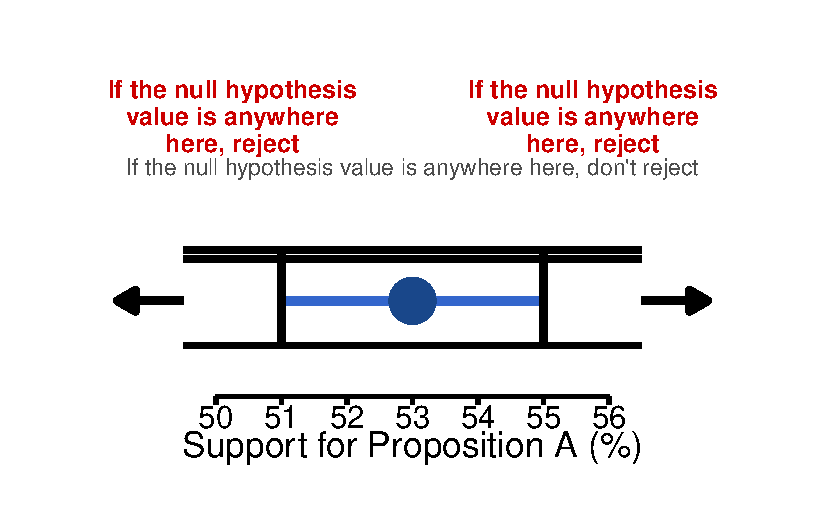
\includegraphics[keepaspectratio]{index_files/figure-pdf/unnamed-chunk-52-1.pdf}}

A practical decision rule for hypothesis testing using confidence
intervals cabe illustrated in the figure above Imagine we conducted a
survey to estimate support for Proposition A, and our 95\% confidence
interval ranges from 51\% to 55\%, with our best estimate (the point
estimate) at 53\%. The key insight is this: if the null hypothesis value
falls inside this confidence interval---anywhere between 51\% and
55\%---we do not reject the null hypothesis. However, if the null
hypothesis value falls outside this range---either below 51\% or above
55\% (shown in the red rejection regions)---we reject the null
hypothesis at the .05 significance level. For example, if our null
hypothesis claimed that support was 50\%, we would reject it because
50\% falls in the left rejection region. Conversely, if the null
hypothesis claimed support was 52\%, we would not reject it because 52\%
falls comfortably within our confidence interval. This visual method
provides an intuitive way to connect confidence intervals with
hypothesis testing decisions: when the null value is captured by your
interval, you lack sufficient evidence to reject it; when it falls
outside, you have enough evidence to reject it.

\section{\texorpdfstring{Connecting Confidence Intervals to \(p\)
Values}{Connecting Confidence Intervals to p Values}}\label{connecting-confidence-intervals-to-p-values}

Several key relationships emerge between CIs and \(p\) values:

\begin{itemize}
\tightlist
\item
  When a null hypothesis value falls outside the 95\% CI, the
  corresponding \(p\) value is less than .05. Since \(p\) falls below
  the significance level, we reject the null hypothesis.
\item
  Conversely, when the null hypothesis value falls within the 95\% CI,
  the \(p\) value exceeds .05, and we fail to reject the null
  hypothesis.
\end{itemize}

When employing .05 as our significance level, the decision rule becomes
straightforward: observe whether the null hypothesis value falls within
or beyond the CI boundaries. A value outside the interval leads us to
reject the null hypothesis and declare the effect statistically
significant; a value inside means we don't reject.

Consider these questions: Could we reject a null hypothesis proposing
50.5\% population support? What about 60\%? Or 52\%? Examine where these
values appear in the figure above?

You likely reasoned correctly---the first two null hypotheses merit
rejection because both values lie outside the CI shown in Figure 6.3.
The third cannot be rejected since 52\% falls within the interval.

We'll explore the translation between CIs and \(p\) values more
thoroughly later, including how to work with significance levels other
than .05.

The figure above reveals that \(p = .05\) when the null hypothesis value
coincides with either CI limit. But what about \(p\) values for other
null hypothesis values? Figure 6.4 illustrates how \(p\) varies
approximately for null hypothesis values positioned at different
locations relative to the CI.

A null hypothesis of 50\%---where the cat's eye appears thin and lies
well beyond the CI---yields \(p = .003\), providing substantial evidence
against that hypothesis. In contrast, consider a null hypothesis of
52\%. If 52\% truly represents population support, then observing
approximately 53\% support in our poll would be quite probable,
resulting in a large \(p\) value: specifically, \(p = .33\). At 52\%,
the cat's eye appears relatively thick.

This pattern holds consistently: thick regions of the cat's eye
correspond to large \(p\) values, indicating little evidence against
those null hypothesis values. As we examine values increasingly distant
from 53\%, the cat's eye narrows, \(p\) values decrease, and evidence
against those null hypothesis values strengthens progressively.

The relationship is clear: the width of the cat's-eye encodes
plausibility, and it narrows as the evidential force of the \(p\) value
increases. Around 52\%--54\%, where the eye is thickest, \(p\) shows
virtually no evidence against those parameter values. As we move away
from 53\% toward and past the CI limits --- where the eye tightens ---
the corresponding \(p\) values register increasingly strong evidence
against those values. Once again the cat's-eye display is doing powerful
conceptual work: one can read it either as a visualization of
plausibility or, equivalently, as a visualization of evidential strength
via \(p\) values. The two views coincide precisely, as they should.

Now consider a null hypothesis proposing 51.5\% population support. How
plausible does this value appear? What \(p\) value would you estimate
for our poll results given this null hypothesis? What evidence do our
data provide against this hypothesis?

\section{p Values and the Normal
Distribution}\label{p-values-and-the-normal-distribution}

We've hit an important checkpoint: our first \(p\) value. No parade
needed---but it's worth noting. I'll use the conventional symbols: the
null hypothesis is \(H_0\) and its hypothesized value is \(\mu_0\). To
illustrate how the \(p\) value is computed, we'll work through the HEAT
example. Mirroring the confidence-interval workflow from Chapter 5,
we'll start with a normal-theory model that treats \(\sigma\) as known,
and then switch to a second model based on the \(t\) distribution that
relaxes that assumption.

\section{\texorpdfstring{Definition of a \(p\)
Value}{Definition of a p Value}}\label{definition-of-a-p-value}

A \(p\) value is the probability --- evaluated under a specified
statistical model --- of observing the result we obtained, or a result
even further from what \(H_0\) predicts, assuming the null hypothesis is
true. Notice the refinement relative to the earlier, more informal
description that spoke of ``results similar to ours.'' The formal
definition replaces ``similar'' with ``as or more extreme.'' A result is
``more extreme'' if it departs even further from the value posited by
\(H_0\), and therefore would constitute at least as much, or more,
evidence against the null than our observed result.

Why include more-extreme hypothetical results when computing the \(p\)
value? Because the goal is to measure the full probability mass of
outcomes that would put the same or greater strain on the null as the
actual data do --- that is, outcomes that would be at least as
surprising if \(H_0\) were in fact correct.

To make this concrete, consider HEAT scores at College Alpha and compare
them to the overall college-student population. Assume HEAT scores
across all college students follow a normal distribution with
\(\mu = 50\) and \(\sigma = 20\). The null hypothesis asserts that
College Alpha's population mean matches the overall mean:
\(H_0!:\ \mu = 50\).

Imagine drawing a sample of \(N = 30\) students from College Alpha and
obtaining a sample mean of \(M = 57.8\). The observed mean is therefore
7.8 points above the null value. The corresponding \(p\) value is the
probability that, under \(H_0\) (i.e., assuming \(\mu = 50\)), a study
patterned like ours would produce a sample mean of \(57.8\) or higher
--- or, by symmetry, \(42.2\) or lower. Those are the outcomes at least
as incompatible with the null as what we observed.

\begin{equation}\phantomsection\label{eq-z-score}{
z = \frac{M - \mu}{\sigma/\sqrt{N}}
}\end{equation}

When \(H_0\) holds true, the population mean equals \(\mu_0\).
Substituting this into Equation~\ref{eq-z-score} yields:

\begin{equation}\phantomsection\label{eq-z-null}{
z = \frac{M - \mu_0}{\sigma/\sqrt{N}}
}\end{equation}

This \(z\) statistic reports how many standard errors the sample mean
(\(M=57.8\)) lies above the null value \(\mu_0 = 50\); it encodes the
degree to which the observed mean departs from what \(H_0\) asserts. The
associated \(p\) value is the probability, under \(H_0\), of obtaining a
deviation of that magnitude or larger in either direction.

Figure 6.5 shows the standard normal distribution with vertical markers
at \(z = 2.136\) and \(z = -2.136\), highlighting the two tail areas
that count as ``as or more extreme'' outcomes. To produce that
illustration I opened the Normal module, selected Two tails and Areas,
and positioned the slider. The combined shaded area equals \(0.0327\).
That is our \(p\) value; rounding yields \(p \approx .03\). Thus,
\(p = .03\) is the probability of producing a \(z\) score of \(2.136\)
or larger in absolute value from a standard normal distribution. In
terms of the raw scale, this corresponds to the probability of observing
\(M \ge 57.8\) or \(M \le 42.2\) if the true mean is 50.

What does a \(p\) value near .03 imply for \(H_0\)? If \(H_0\) were
correct, only about 3\% of studies of this design would generate a mean
at least this far from 50. This makes the observed result unusual under
the null and therefore counts as evidence against \(H_0\). Under
standard NHST conventions, \(p < .05\) leads us to reject the claim that
College Alpha's population mean equals 50 and to infer instead that
their mean HEAT score is higher. In the next exercise we will examine
the confidence interval associated with this result.

Here's a systematic summary of how we determined and interpreted that
\(p\) value:

\begin{enumerate}
\def\labelenumi{\arabic{enumi}.}
\item
  We specified our sample result (\(M = 57.8\)) and our null hypothesis
  (\(H_0: \mu = 50\)).
\item
  We examined the difference, or discrepancy, between that result and
  the null hypothesis value. Our difference was \((57.8 - 50)\).
\end{enumerate}

\begin{Shaded}
\begin{Highlighting}[]
\FunctionTok{library}\NormalTok{(ggplot2)}
\FunctionTok{library}\NormalTok{(dplyr)}
\FunctionTok{library}\NormalTok{(tidyr)}

\CommentTok{\# Prepare data with sample sizes}
\NormalTok{agg2 }\OtherTok{\textless{}{-}} \FunctionTok{as.data.frame}\NormalTok{(}\FunctionTok{margin.table}\NormalTok{(UCBAdmissions, }\FunctionTok{c}\NormalTok{(}\DecValTok{1}\NormalTok{, }\DecValTok{2}\NormalTok{))) }\SpecialCharTok{|\textgreater{}}
  \FunctionTok{pivot\_wider}\NormalTok{(}\AttributeTok{names\_from =}\NormalTok{ Admit, }\AttributeTok{values\_from =}\NormalTok{ Freq) }\SpecialCharTok{|\textgreater{}}
  \FunctionTok{mutate}\NormalTok{(}
    \AttributeTok{n =}\NormalTok{ Admitted }\SpecialCharTok{+}\NormalTok{ Rejected,}
    \AttributeTok{pct =}\NormalTok{ Admitted }\SpecialCharTok{/}\NormalTok{ n,}
    \AttributeTok{se =} \FunctionTok{sqrt}\NormalTok{(pct }\SpecialCharTok{*}\NormalTok{ (}\DecValTok{1} \SpecialCharTok{{-}}\NormalTok{ pct) }\SpecialCharTok{/}\NormalTok{ n),}
    \AttributeTok{label =} \FunctionTok{paste0}\NormalTok{(scales}\SpecialCharTok{::}\FunctionTok{percent}\NormalTok{(pct, }\AttributeTok{accuracy =} \FloatTok{0.1}\NormalTok{), }\StringTok{"}\SpecialCharTok{\textbackslash{}n}\StringTok{(n="}\NormalTok{, scales}\SpecialCharTok{::}\FunctionTok{comma}\NormalTok{(n), }\StringTok{")"}\NormalTok{)}
\NormalTok{  )}

\NormalTok{bold\_pal }\OtherTok{\textless{}{-}} \FunctionTok{c}\NormalTok{(}\StringTok{"Female"} \OtherTok{=} \StringTok{"\#FF1493"}\NormalTok{, }\StringTok{"Male"} \OtherTok{=} \StringTok{"\#00CED1"}\NormalTok{)}

\FunctionTok{ggplot}\NormalTok{(agg2, }\FunctionTok{aes}\NormalTok{(}\AttributeTok{x =}\NormalTok{ Gender, }\AttributeTok{y =}\NormalTok{ pct, }\AttributeTok{fill =}\NormalTok{ Gender)) }\SpecialCharTok{+}
  \FunctionTok{geom\_errorbar}\NormalTok{(}
    \FunctionTok{aes}\NormalTok{(}\AttributeTok{ymin =}\NormalTok{ pct }\SpecialCharTok{{-}} \FloatTok{1.96} \SpecialCharTok{*}\NormalTok{ se, }\AttributeTok{ymax =}\NormalTok{ pct }\SpecialCharTok{+} \FloatTok{1.96} \SpecialCharTok{*}\NormalTok{ se),}
    \AttributeTok{width =} \FloatTok{0.2}\NormalTok{,}
    \AttributeTok{linewidth =} \DecValTok{1}\NormalTok{,}
    \AttributeTok{color =} \StringTok{"grey20"}
\NormalTok{  ) }\SpecialCharTok{+}
  \FunctionTok{geom\_col}\NormalTok{(}
    \AttributeTok{width =} \FloatTok{0.75}\NormalTok{,}
    \AttributeTok{color =} \StringTok{"white"}\NormalTok{,}
    \AttributeTok{linewidth =} \DecValTok{2}\NormalTok{,}
    \AttributeTok{alpha =} \FloatTok{0.95}
\NormalTok{  ) }\SpecialCharTok{+}
  \FunctionTok{geom\_text}\NormalTok{(}
    \FunctionTok{aes}\NormalTok{(}\AttributeTok{label =}\NormalTok{ label),}
    \AttributeTok{vjust =} \SpecialCharTok{{-}}\FloatTok{2.2}\NormalTok{,}
    \AttributeTok{size =} \DecValTok{5}\NormalTok{,}
    \AttributeTok{fontface =} \StringTok{"bold"}\NormalTok{,}
    \AttributeTok{color =} \StringTok{"grey10"}\NormalTok{,}
    \AttributeTok{lineheight =} \FloatTok{0.9}
\NormalTok{  ) }\SpecialCharTok{+}
  
  \FunctionTok{scale\_y\_continuous}\NormalTok{(}
    \AttributeTok{labels =}\NormalTok{ scales}\SpecialCharTok{::}\FunctionTok{percent\_format}\NormalTok{(}\AttributeTok{accuracy =} \DecValTok{1}\NormalTok{),}
    \AttributeTok{limits =} \FunctionTok{c}\NormalTok{(}\DecValTok{0}\NormalTok{, }\FloatTok{0.55}\NormalTok{),}
    \AttributeTok{breaks =} \FunctionTok{seq}\NormalTok{(}\DecValTok{0}\NormalTok{, }\FloatTok{0.5}\NormalTok{, }\FloatTok{0.1}\NormalTok{),}
    \AttributeTok{expand =} \FunctionTok{expansion}\NormalTok{(}\AttributeTok{mult =} \FunctionTok{c}\NormalTok{(}\DecValTok{0}\NormalTok{, }\FloatTok{0.02}\NormalTok{))}
\NormalTok{  ) }\SpecialCharTok{+}
  \FunctionTok{scale\_fill\_manual}\NormalTok{(}\AttributeTok{values =}\NormalTok{ bold\_pal) }\SpecialCharTok{+}
  \CommentTok{\# Labels}
  \FunctionTok{labs}\NormalTok{(}
    \AttributeTok{title =} \StringTok{"Gender Disparity in UC Berkeley Admissions"}\NormalTok{,}
    \AttributeTok{subtitle =} \StringTok{"Overall admission rates mask department{-}level patterns (Fall 1973)"}\NormalTok{,}
    \AttributeTok{x =} \ConstantTok{NULL}\NormalTok{,}
    \AttributeTok{y =} \StringTok{"Admission rate (\%)"}\NormalTok{,}
    \AttributeTok{caption =} \StringTok{"Error bars represent 95\% confidence intervals"}
\NormalTok{  ) }\SpecialCharTok{+}

  \FunctionTok{theme\_minimal}\NormalTok{(}\AttributeTok{base\_size =} \DecValTok{13}\NormalTok{, }\AttributeTok{base\_family =} \StringTok{"sans"}\NormalTok{) }\SpecialCharTok{+}
  \FunctionTok{theme}\NormalTok{(}

    \AttributeTok{plot.background =} \FunctionTok{element\_rect}\NormalTok{(}\AttributeTok{fill =} \StringTok{"white"}\NormalTok{, }\AttributeTok{color =} \ConstantTok{NA}\NormalTok{),}
    \AttributeTok{panel.background =} \FunctionTok{element\_rect}\NormalTok{(}\AttributeTok{fill =} \StringTok{"white"}\NormalTok{, }\AttributeTok{color =} \ConstantTok{NA}\NormalTok{),}
    \AttributeTok{panel.grid =} \FunctionTok{element\_blank}\NormalTok{(),  }\CommentTok{\# Remove ALL gridlines}
    

    \AttributeTok{axis.line =} \FunctionTok{element\_line}\NormalTok{(}\AttributeTok{color =} \StringTok{"grey20"}\NormalTok{, }\AttributeTok{linewidth =} \FloatTok{0.8}\NormalTok{),}
    \AttributeTok{axis.ticks =} \FunctionTok{element\_line}\NormalTok{(}\AttributeTok{color =} \StringTok{"grey20"}\NormalTok{, }\AttributeTok{linewidth =} \FloatTok{0.6}\NormalTok{),}
    \AttributeTok{axis.ticks.length =} \FunctionTok{unit}\NormalTok{(}\FloatTok{0.25}\NormalTok{, }\StringTok{"cm"}\NormalTok{),}
    \AttributeTok{axis.text =} \FunctionTok{element\_text}\NormalTok{(}\AttributeTok{color =} \StringTok{"grey10"}\NormalTok{, }\AttributeTok{size =} \DecValTok{12}\NormalTok{, }\AttributeTok{face =} \StringTok{"bold"}\NormalTok{),}
    \AttributeTok{axis.text.x =} \FunctionTok{element\_text}\NormalTok{(}\AttributeTok{size =} \DecValTok{14}\NormalTok{),}
    \AttributeTok{axis.title.y =} \FunctionTok{element\_text}\NormalTok{(}\AttributeTok{face =} \StringTok{"bold"}\NormalTok{, }\AttributeTok{size =} \DecValTok{13}\NormalTok{, }\AttributeTok{margin =} \FunctionTok{margin}\NormalTok{(}\AttributeTok{r =} \DecValTok{12}\NormalTok{)),}
    
    \AttributeTok{plot.title =} \FunctionTok{element\_text}\NormalTok{(}
      \AttributeTok{face =} \StringTok{"bold"}\NormalTok{,}
      \AttributeTok{size =} \DecValTok{17}\NormalTok{,}
      \AttributeTok{hjust =} \DecValTok{0}\NormalTok{,}
      \AttributeTok{margin =} \FunctionTok{margin}\NormalTok{(}\AttributeTok{b =} \DecValTok{6}\NormalTok{),}
      \AttributeTok{color =} \StringTok{"grey10"}
\NormalTok{    ),}
    \AttributeTok{plot.subtitle =} \FunctionTok{element\_text}\NormalTok{(}
      \AttributeTok{size =} \DecValTok{11}\NormalTok{,}
      \AttributeTok{hjust =} \DecValTok{0}\NormalTok{,}
      \AttributeTok{margin =} \FunctionTok{margin}\NormalTok{(}\AttributeTok{b =} \DecValTok{18}\NormalTok{),}
      \AttributeTok{color =} \StringTok{"grey40"}
\NormalTok{    ),}
    \AttributeTok{plot.caption =} \FunctionTok{element\_text}\NormalTok{(}
      \AttributeTok{size =} \DecValTok{9}\NormalTok{,}
      \AttributeTok{hjust =} \DecValTok{1}\NormalTok{,}
      \AttributeTok{margin =} \FunctionTok{margin}\NormalTok{(}\AttributeTok{t =} \DecValTok{12}\NormalTok{),}
      \AttributeTok{color =} \StringTok{"grey50"}\NormalTok{,}
      \AttributeTok{face =} \StringTok{"italic"}
\NormalTok{    ),}
    

    \AttributeTok{legend.position =} \StringTok{"none"}\NormalTok{,}
    

    \AttributeTok{plot.margin =} \FunctionTok{margin}\NormalTok{(}\DecValTok{25}\NormalTok{, }\DecValTok{25}\NormalTok{, }\DecValTok{20}\NormalTok{, }\DecValTok{25}\NormalTok{)}
\NormalTok{  )}
\end{Highlighting}
\end{Shaded}

\pandocbounded{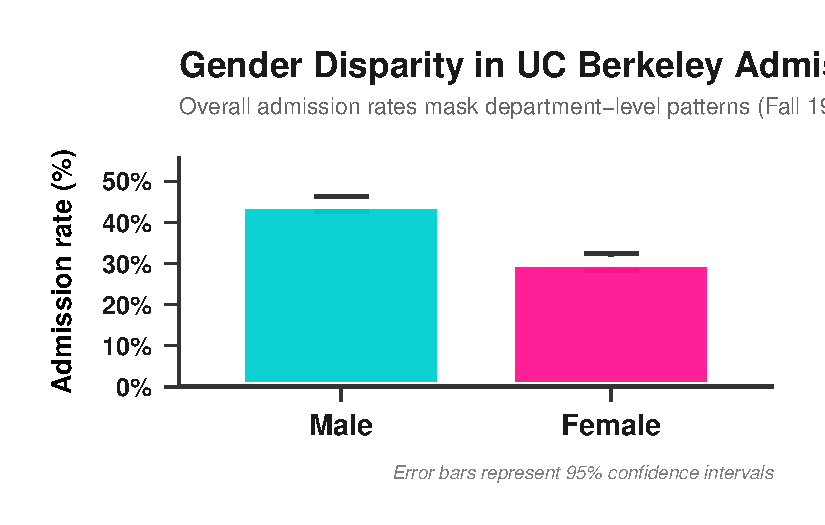
\includegraphics[keepaspectratio]{index_files/figure-pdf/unnamed-chunk-53-1.pdf}}

\begin{enumerate}
\def\labelenumi{\arabic{enumi}.}
\setcounter{enumi}{2}
\item
  We applied a formula (Equation~\ref{eq-z-null}) to compute the value
  of a \emph{test statistic} from that difference, assuming \(H_0\) were
  true. We determined that \(z = 2.136\).
\item
  We examined the distribution of the test statistic, \(z\), to identify
  the two tail areas corresponding to that test statistic value. Figure
  6.5 reveals that the combined area is .03 (after rounding); this
  constitutes our \(p\) value.
\item
  We interpreted the \(p\) value, employing either the NHST framework or
  the strength of evidence approach.
\end{enumerate}

\begin{tcolorbox}[enhanced jigsaw, colframe=quarto-callout-note-color-frame, left=2mm, leftrule=.75mm, rightrule=.15mm, opacityback=0, arc=.35mm, colback=white, bottomrule=.15mm, breakable, toprule=.15mm]
\begin{minipage}[t]{5.5mm}
\textcolor{quarto-callout-note-color}{\faInfo}
\end{minipage}%
\begin{minipage}[t]{\textwidth - 5.5mm}

\vspace{-3mm}\textbf{Test Statistic}\vspace{3mm}

A \emph{test statistic} is any summary of the data whose sampling
distribution is known under \(H_0\) and that can therefore be used to
compute a \(p\) value. A familiar example is the \(z\) statistic,
which---under its assumptions---follows the standard normal
distribution.

\end{minipage}%
\end{tcolorbox}

Using the same sample mean can yield different \(p\) values because the
underlying statistical models differ. If it is defensible to treat the
population standard deviation for College Alpha as known---for example,
\(\sigma = 20\)---we adopt the normal-theory model and use \(z\) to
obtain the \(p\) value. If, instead, we hesitate to import
\(\sigma = 20\) from the broader college population (because College
Alpha may differ in relevant ways), we avoid fixing \(\sigma\) and work
with the \(t\) model, substituting the sample standard deviation \(s\)
and using the \(t\) statistic (and its degrees of freedom) to compute
the \(p\) value or the CI. As so often in applied work, this is a
judgment call. When a trustworthy population value of \(\sigma\) is
available, it is typically preferable to use it. Relying on \(s\) is
more fragile when \(N\) is small, because \(s\) can be a noisy estimate
of \(\sigma\); in those situations the \(t\) approach appropriately
accounts for that extra uncertainty.

The fundamental distinction, naturally, lies in the fact that the two
approaches rely on different statistical models. If we deem it
reasonable to apply the population value of \(\sigma = 20\) for College
Alpha students, then we select a normal distribution model and employ
\(z\) to compute the \(p\) value. However, if we consider students at
that institution to be sufficiently different from the broader college
population to which the HEAT applies, then we might prefer to avoid
assuming \(\sigma = 20\) for College Alpha students. In this case, we
would select a \(t\) distribution model and utilize \(s\) and \(t\) to
calculate the \(p\) value (or CI). As is frequently the case, this
represents a matter of informed professional judgment. We will typically
prefer to use a known population value of \(\sigma\) when available,
rather than relying on our sample \(s\) as an estimate of \(\sigma\),
particularly when \(N\) is small and consequently our \(s\) may not
provide a reliable estimate of \(\sigma\).

We've explored four methods for interpreting a CI. If the null
hypothesis value \(\mu_0\) falls outside or inside the CI to determine
whether \(p < .05\) or \(p > .05\). Here I'll extend this further and
examine how to approximate a \(p\) value visually, given a 95\% CI and a
null hypothesis value \(\mu_0\).

\begin{Shaded}
\begin{Highlighting}[]
\CommentTok{\#| label: fig{-}ci{-}p{-}value{-}guidelines}
\CommentTok{\#| fig{-}cap: "Four sample means with 95\% CIs, same length. The null value is $\textbackslash{}\textbackslash{}mu\_0$. Red labels show approximate $p$ values; cream callouts show MoE heuristics."}
\CommentTok{\#| fig{-}width: 10}
\CommentTok{\#| fig{-}height: 6}
\CommentTok{\#| fig{-}format: png}
\CommentTok{\#| fig{-}dpi: 300}
\CommentTok{\#| warning: false}
\CommentTok{\#| message: false}

\FunctionTok{suppressPackageStartupMessages}\NormalTok{(}\FunctionTok{library}\NormalTok{(ggplot2))}
\FunctionTok{library}\NormalTok{(grid)  }\CommentTok{\# for unit()}

\CommentTok{\# {-}{-}{-}{-}{-}{-}{-}{-}{-}{-}{-}{-}{-}{-}{-}{-}{-}{-}{-}{-}{-}{-}{-}{-}{-}}
\CommentTok{\# Helper: draw a curly brace with two smooth curves}
\CommentTok{\# {-}{-}{-}{-}{-}{-}{-}{-}{-}{-}{-}{-}{-}{-}{-}{-}{-}{-}{-}{-}{-}{-}{-}{-}{-}}
\NormalTok{brace }\OtherTok{\textless{}{-}} \ControlFlowTok{function}\NormalTok{(x, y0, y1, }\AttributeTok{w =} \FloatTok{0.20}\NormalTok{, }\AttributeTok{col =} \StringTok{"black"}\NormalTok{, }\AttributeTok{lwd =} \FloatTok{0.9}\NormalTok{)\{}
\NormalTok{  ym }\OtherTok{\textless{}{-}}\NormalTok{ (y0 }\SpecialCharTok{+}\NormalTok{ y1) }\SpecialCharTok{/} \DecValTok{2}
  \FunctionTok{list}\NormalTok{(}
    \FunctionTok{annotate}\NormalTok{(}\StringTok{"curve"}\NormalTok{, }\AttributeTok{x =}\NormalTok{ x,   }\AttributeTok{y =}\NormalTok{ ym, }\AttributeTok{xend =}\NormalTok{ x }\SpecialCharTok{+}\NormalTok{ w, }\AttributeTok{yend =}\NormalTok{ y1,}
             \AttributeTok{curvature =} \FloatTok{0.55}\NormalTok{, }\AttributeTok{colour =}\NormalTok{ col, }\AttributeTok{linewidth =}\NormalTok{ lwd),}
    \FunctionTok{annotate}\NormalTok{(}\StringTok{"curve"}\NormalTok{, }\AttributeTok{x =}\NormalTok{ x,   }\AttributeTok{y =}\NormalTok{ ym, }\AttributeTok{xend =}\NormalTok{ x }\SpecialCharTok{+}\NormalTok{ w, }\AttributeTok{yend =}\NormalTok{ y0,}
             \AttributeTok{curvature =} \SpecialCharTok{{-}}\FloatTok{0.55}\NormalTok{, }\AttributeTok{colour =}\NormalTok{ col, }\AttributeTok{linewidth =}\NormalTok{ lwd)}
\NormalTok{  )}
\NormalTok{\}}

\CommentTok{\# {-}{-}{-}{-}{-}{-}{-}{-}{-}{-}{-}{-}{-}{-}{-}{-}{-}{-}{-}{-}{-}{-}{-}{-}{-}}
\CommentTok{\# Data \& parameters}
\CommentTok{\# {-}{-}{-}{-}{-}{-}{-}{-}{-}{-}{-}{-}{-}{-}{-}{-}{-}{-}{-}{-}{-}{-}{-}{-}{-}}
\NormalTok{moe }\OtherTok{\textless{}{-}} \DecValTok{2}
\NormalTok{mu0 }\OtherTok{\textless{}{-}} \DecValTok{0}

\NormalTok{sc }\OtherTok{\textless{}{-}} \FunctionTok{data.frame}\NormalTok{(}
  \AttributeTok{x     =} \DecValTok{1}\SpecialCharTok{:}\DecValTok{4}\NormalTok{,}
  \AttributeTok{label =} \FunctionTok{c}\NormalTok{(}\StringTok{"Guideline 1"}\NormalTok{,}\StringTok{"Guideline 2"}\NormalTok{,}\StringTok{"Guideline 3"}\NormalTok{,}\StringTok{"Guideline 4"}\NormalTok{),}
  \AttributeTok{M     =} \FunctionTok{c}\NormalTok{(}\FloatTok{0.65}\NormalTok{, }\FloatTok{2.00}\NormalTok{, }\FloatTok{2.60}\NormalTok{, }\FloatTok{3.30}\NormalTok{),}
  \AttributeTok{p\_lab =} \FunctionTok{c}\NormalTok{(}\StringTok{".20"}\NormalTok{,}\StringTok{".05"}\NormalTok{,}\StringTok{".01"}\NormalTok{,}\StringTok{".001"}\NormalTok{)}
\NormalTok{)}
\NormalTok{sc}\SpecialCharTok{$}\NormalTok{lo }\OtherTok{\textless{}{-}}\NormalTok{ sc}\SpecialCharTok{$}\NormalTok{M }\SpecialCharTok{{-}}\NormalTok{ moe}
\NormalTok{sc}\SpecialCharTok{$}\NormalTok{hi }\OtherTok{\textless{}{-}}\NormalTok{ sc}\SpecialCharTok{$}\NormalTok{M }\SpecialCharTok{+}\NormalTok{ moe}

\CommentTok{\# Palette}
\NormalTok{col\_line  }\OtherTok{\textless{}{-}} \StringTok{"red"}
\NormalTok{col\_point }\OtherTok{\textless{}{-}} \StringTok{"\#1F3B73"}
\NormalTok{col\_text  }\OtherTok{\textless{}{-}} \StringTok{"\#1F1F1F"}
\NormalTok{col\_red   }\OtherTok{\textless{}{-}} \StringTok{"\#B52A2A"}
\NormalTok{col\_box   }\OtherTok{\textless{}{-}} \StringTok{"\#FFF6C8"}

\CommentTok{\# Canvas (extra right room so labels never collide)}
\NormalTok{y\_min }\OtherTok{\textless{}{-}} \SpecialCharTok{{-}}\FloatTok{4.6}\NormalTok{; y\_max }\OtherTok{\textless{}{-}} \FloatTok{7.0}
\NormalTok{x\_min }\OtherTok{\textless{}{-}} \SpecialCharTok{{-}}\FloatTok{0.8}\NormalTok{; x\_max }\OtherTok{\textless{}{-}} \FloatTok{7.0}
\NormalTok{yticks }\OtherTok{\textless{}{-}} \FunctionTok{seq}\NormalTok{(}\SpecialCharTok{{-}}\DecValTok{4}\NormalTok{, }\DecValTok{6}\NormalTok{, }\AttributeTok{by =} \DecValTok{1}\NormalTok{)}

\CommentTok{\# Callout positions (chosen to avoid *any* overlap)}
\NormalTok{moe\_box\_xy  }\OtherTok{\textless{}{-}} \FunctionTok{c}\NormalTok{(}\FloatTok{5.55}\NormalTok{, }\FloatTok{5.65}\NormalTok{)   }\CommentTok{\# x, y}
\NormalTok{moe\_lead\_xy }\OtherTok{\textless{}{-}} \FunctionTok{matrix}\NormalTok{(}\FunctionTok{c}\NormalTok{(}\FloatTok{5.25}\NormalTok{, }\FloatTok{5.55}\NormalTok{, }\FloatTok{4.18}\NormalTok{, }\FloatTok{4.60}\NormalTok{), }\AttributeTok{ncol =} \DecValTok{2}\NormalTok{, }\AttributeTok{byrow =} \ConstantTok{TRUE}\NormalTok{) }\CommentTok{\# (x,y){-}\textgreater{}(xend,yend)}

\NormalTok{p23\_box\_xy  }\OtherTok{\textless{}{-}} \FunctionTok{c}\NormalTok{(}\FloatTok{5.40}\NormalTok{, }\FloatTok{3.95}\NormalTok{)}
\NormalTok{p23\_lead\_xy }\OtherTok{\textless{}{-}} \FunctionTok{matrix}\NormalTok{(}\FunctionTok{c}\NormalTok{(}\FloatTok{5.00}\NormalTok{, }\FloatTok{3.85}\NormalTok{, }\FloatTok{3.18}\NormalTok{, sc}\SpecialCharTok{$}\NormalTok{M[}\DecValTok{3}\NormalTok{] }\SpecialCharTok{+}\NormalTok{ (}\DecValTok{2}\SpecialCharTok{/}\DecValTok{3}\NormalTok{)}\SpecialCharTok{*}\NormalTok{moe }\SpecialCharTok{+} \FloatTok{0.04}\NormalTok{), }\AttributeTok{ncol =} \DecValTok{2}\NormalTok{, }\AttributeTok{byrow =} \ConstantTok{TRUE}\NormalTok{)}

\NormalTok{p13\_box\_xy  }\OtherTok{\textless{}{-}} \FunctionTok{c}\NormalTok{(}\FloatTok{4.95}\NormalTok{, }\SpecialCharTok{{-}}\FloatTok{1.10}\NormalTok{)}
\NormalTok{p13\_lead\_xy }\OtherTok{\textless{}{-}} \FunctionTok{matrix}\NormalTok{(}\FunctionTok{c}\NormalTok{(}\FloatTok{1.18}\NormalTok{, mu0 }\SpecialCharTok{{-}} \FloatTok{0.12}\NormalTok{, }\FloatTok{4.35}\NormalTok{, }\SpecialCharTok{{-}}\FloatTok{0.92}\NormalTok{), }\AttributeTok{ncol =} \DecValTok{2}\NormalTok{, }\AttributeTok{byrow =} \ConstantTok{TRUE}\NormalTok{)}

\FunctionTok{ggplot}\NormalTok{() }\SpecialCharTok{+}
  \CommentTok{\# Left axis + ticks}
  \FunctionTok{annotate}\NormalTok{(}\StringTok{"segment"}\NormalTok{, }\AttributeTok{x =} \DecValTok{0}\NormalTok{, }\AttributeTok{xend =} \DecValTok{0}\NormalTok{, }\AttributeTok{y =}\NormalTok{ y\_min, }\AttributeTok{yend =}\NormalTok{ y\_max,}
           \AttributeTok{linewidth =} \FloatTok{0.9}\NormalTok{, }\AttributeTok{colour =} \StringTok{"black"}\NormalTok{) }\SpecialCharTok{+}
  \FunctionTok{annotate}\NormalTok{(}\StringTok{"segment"}\NormalTok{, }\AttributeTok{x =} \DecValTok{0}\NormalTok{, }\AttributeTok{xend =} \FloatTok{0.12}\NormalTok{, }\AttributeTok{y =}\NormalTok{ yticks, }\AttributeTok{yend =}\NormalTok{ yticks,}
           \AttributeTok{linewidth =} \FloatTok{0.6}\NormalTok{, }\AttributeTok{colour =} \StringTok{"black"}\NormalTok{) }\SpecialCharTok{+}

  \CommentTok{\# Baseline at mu0 + label}
  \FunctionTok{geom\_hline}\NormalTok{(}\AttributeTok{yintercept =}\NormalTok{ mu0, }\AttributeTok{linewidth =} \FloatTok{0.3}\NormalTok{, }\AttributeTok{colour =} \StringTok{"grey25"}\NormalTok{) }\SpecialCharTok{+}
  \FunctionTok{annotate}\NormalTok{(}\StringTok{"text"}\NormalTok{, }\AttributeTok{x =} \SpecialCharTok{{-}}\FloatTok{0.10}\NormalTok{, }\AttributeTok{y =}\NormalTok{ mu0, }\AttributeTok{label =} \StringTok{"mu[0]"}\NormalTok{,}
           \AttributeTok{parse =} \ConstantTok{TRUE}\NormalTok{, }\AttributeTok{hjust =} \DecValTok{1}\NormalTok{, }\AttributeTok{vjust =} \FloatTok{0.25}\NormalTok{, }\AttributeTok{size =} \FloatTok{6.2}\NormalTok{, }\AttributeTok{colour =} \StringTok{"black"}\NormalTok{) }\SpecialCharTok{+}

  \CommentTok{\# Y{-}axis title}
  \FunctionTok{annotate}\NormalTok{(}\StringTok{"text"}\NormalTok{, }\AttributeTok{x =} \SpecialCharTok{{-}}\FloatTok{0.55}\NormalTok{, }\AttributeTok{y =} \FloatTok{3.0}\NormalTok{, }\AttributeTok{label =} \StringTok{"Dependent Variable"}\NormalTok{,}
           \AttributeTok{angle =} \DecValTok{90}\NormalTok{, }\AttributeTok{size =} \FloatTok{5.8}\NormalTok{, }\AttributeTok{fontface =} \StringTok{"bold"}\NormalTok{, }\AttributeTok{colour =}\NormalTok{ col\_text) }\SpecialCharTok{+}

  \CommentTok{\# CI pillars + short caps}
  \FunctionTok{geom\_segment}\NormalTok{(}\AttributeTok{data =}\NormalTok{ sc, }\FunctionTok{aes}\NormalTok{(}\AttributeTok{x =}\NormalTok{ x, }\AttributeTok{xend =}\NormalTok{ x, }\AttributeTok{y =}\NormalTok{ lo, }\AttributeTok{yend =}\NormalTok{ hi),}
               \AttributeTok{linewidth =} \FloatTok{2.2}\NormalTok{, }\AttributeTok{colour =}\NormalTok{ col\_line, }\AttributeTok{lineend =} \StringTok{"butt"}\NormalTok{) }\SpecialCharTok{+}
  \FunctionTok{geom\_segment}\NormalTok{(}\AttributeTok{data =}\NormalTok{ sc, }\FunctionTok{aes}\NormalTok{(}\AttributeTok{x =}\NormalTok{ x, }\AttributeTok{xend =}\NormalTok{ x, }\AttributeTok{y =}\NormalTok{ hi, }\AttributeTok{yend =}\NormalTok{ hi }\SpecialCharTok{+} \FloatTok{0.45}\NormalTok{),}
               \AttributeTok{linewidth =} \FloatTok{1.2}\NormalTok{, }\AttributeTok{colour =}\NormalTok{ col\_line) }\SpecialCharTok{+}

  \CommentTok{\# Means + italic M}
  \FunctionTok{geom\_point}\NormalTok{(}\AttributeTok{data =}\NormalTok{ sc, }\FunctionTok{aes}\NormalTok{(}\AttributeTok{x =}\NormalTok{ x, }\AttributeTok{y =}\NormalTok{ M),}
             \AttributeTok{shape =} \DecValTok{16}\NormalTok{, }\AttributeTok{size =} \FloatTok{5.2}\NormalTok{, }\AttributeTok{colour =}\NormalTok{ col\_point) }\SpecialCharTok{+}
  \FunctionTok{geom\_text}\NormalTok{ (}\AttributeTok{data =}\NormalTok{ sc, }\FunctionTok{aes}\NormalTok{(}\AttributeTok{x =}\NormalTok{ x }\SpecialCharTok{{-}} \FloatTok{0.18}\NormalTok{, }\AttributeTok{y =}\NormalTok{ M, }\AttributeTok{label =} \StringTok{"M"}\NormalTok{),}
             \AttributeTok{fontface =} \StringTok{"italic"}\NormalTok{, }\AttributeTok{size =} \FloatTok{5.6}\NormalTok{, }\AttributeTok{colour =}\NormalTok{ col\_text) }\SpecialCharTok{+}

  \CommentTok{\# Guideline titles (staggered to clear callouts)}
  \FunctionTok{geom\_text}\NormalTok{(}\AttributeTok{data =} \FunctionTok{transform}\NormalTok{(sc, }\AttributeTok{ylab =}\NormalTok{ hi }\SpecialCharTok{+} \FunctionTok{c}\NormalTok{(}\FloatTok{0.85}\NormalTok{, }\FloatTok{0.95}\NormalTok{, }\FloatTok{1.05}\NormalTok{, }\FloatTok{1.25}\NormalTok{)),}
            \FunctionTok{aes}\NormalTok{(}\AttributeTok{x =}\NormalTok{ x, }\AttributeTok{y =}\NormalTok{ ylab, }\AttributeTok{label =}\NormalTok{ label),}
            \AttributeTok{fontface =} \StringTok{"plain"}\NormalTok{, }\AttributeTok{size =} \DecValTok{3}\NormalTok{, }\AttributeTok{colour =}\NormalTok{ col\_text) }\SpecialCharTok{+}

  \CommentTok{\# {-}{-}{-} Braces (clean, organized) {-}{-}{-}}
  \CommentTok{\# tiny brace under G1 crossing baseline}
  \FunctionTok{brace}\NormalTok{(}\AttributeTok{x =} \FloatTok{1.00}\NormalTok{, }\AttributeTok{y0 =}\NormalTok{ mu0 }\SpecialCharTok{{-}} \FloatTok{0.95}\NormalTok{, }\AttributeTok{y1 =}\NormalTok{ mu0 }\SpecialCharTok{{-}} \FloatTok{0.20}\NormalTok{, }\AttributeTok{w =} \FloatTok{0.18}\NormalTok{, }\AttributeTok{col =}\NormalTok{ col\_text, }\AttributeTok{lwd =} \FloatTok{0.9}\NormalTok{) }\SpecialCharTok{+}
  \CommentTok{\# brace at G3 where CI crosses baseline}
  \FunctionTok{brace}\NormalTok{(}\AttributeTok{x =} \FloatTok{3.00}\NormalTok{, }\AttributeTok{y0 =}\NormalTok{ mu0 }\SpecialCharTok{{-}} \FloatTok{0.40}\NormalTok{, }\AttributeTok{y1 =}\NormalTok{ mu0 }\SpecialCharTok{+} \FloatTok{0.30}\NormalTok{, }\AttributeTok{w =} \FloatTok{0.18}\NormalTok{, }\AttributeTok{col =}\NormalTok{ col\_text, }\AttributeTok{lwd =} \FloatTok{0.9}\NormalTok{) }\SpecialCharTok{+}
  \CommentTok{\# two braces on G4: lower (mu0→M) and upper (M→upper CI)}
  \FunctionTok{brace}\NormalTok{(}\AttributeTok{x =} \FloatTok{4.00}\NormalTok{, }\AttributeTok{y0 =}\NormalTok{ mu0 }\SpecialCharTok{+} \FloatTok{0.10}\NormalTok{, }\AttributeTok{y1 =}\NormalTok{ sc}\SpecialCharTok{$}\NormalTok{M[}\DecValTok{4}\NormalTok{] }\SpecialCharTok{{-}} \FloatTok{0.05}\NormalTok{, }\AttributeTok{w =} \FloatTok{0.18}\NormalTok{, }\AttributeTok{col =}\NormalTok{ col\_text, }\AttributeTok{lwd =} \FloatTok{1.0}\NormalTok{) }\SpecialCharTok{+}
  \FunctionTok{brace}\NormalTok{(}\AttributeTok{x =} \FloatTok{4.00}\NormalTok{, }\AttributeTok{y0 =}\NormalTok{ sc}\SpecialCharTok{$}\NormalTok{M[}\DecValTok{4}\NormalTok{] }\SpecialCharTok{+} \FloatTok{0.05}\NormalTok{, }\AttributeTok{y1 =}\NormalTok{ sc}\SpecialCharTok{$}\NormalTok{hi[}\DecValTok{4}\NormalTok{],   }\AttributeTok{w =} \FloatTok{0.18}\NormalTok{, }\AttributeTok{col =}\NormalTok{ col\_text, }\AttributeTok{lwd =} \FloatTok{1.0}\NormalTok{) }\SpecialCharTok{+}

  \CommentTok{\# {-}{-}{-} MoE bracket on G4 (for exact endpoints) {-}{-}{-}}
  \FunctionTok{annotate}\NormalTok{(}\StringTok{"segment"}\NormalTok{, }\AttributeTok{x =} \FloatTok{4.12}\NormalTok{, }\AttributeTok{xend =} \FloatTok{4.12}\NormalTok{, }\AttributeTok{y =}\NormalTok{ sc}\SpecialCharTok{$}\NormalTok{M[}\DecValTok{4}\NormalTok{], }\AttributeTok{yend =}\NormalTok{ sc}\SpecialCharTok{$}\NormalTok{hi[}\DecValTok{4}\NormalTok{],}
           \AttributeTok{linewidth =} \FloatTok{0.5}\NormalTok{, }\AttributeTok{colour =} \StringTok{"black"}\NormalTok{) }\SpecialCharTok{+}
  \FunctionTok{annotate}\NormalTok{(}\StringTok{"segment"}\NormalTok{, }\AttributeTok{x =} \FloatTok{4.07}\NormalTok{, }\AttributeTok{xend =} \FloatTok{4.17}\NormalTok{, }\AttributeTok{y =}\NormalTok{ sc}\SpecialCharTok{$}\NormalTok{M[}\DecValTok{4}\NormalTok{],  }\AttributeTok{yend =}\NormalTok{ sc}\SpecialCharTok{$}\NormalTok{M[}\DecValTok{4}\NormalTok{],  }\AttributeTok{linewidth =} \FloatTok{0.5}\NormalTok{) }\SpecialCharTok{+}
  \FunctionTok{annotate}\NormalTok{(}\StringTok{"segment"}\NormalTok{, }\AttributeTok{x =} \FloatTok{4.07}\NormalTok{, }\AttributeTok{xend =} \FloatTok{4.17}\NormalTok{, }\AttributeTok{y =}\NormalTok{ sc}\SpecialCharTok{$}\NormalTok{hi[}\DecValTok{4}\NormalTok{], }\AttributeTok{yend =}\NormalTok{ sc}\SpecialCharTok{$}\NormalTok{hi[}\DecValTok{4}\NormalTok{], }\AttributeTok{linewidth =} \FloatTok{0.5}\NormalTok{) }\SpecialCharTok{+}

  \CommentTok{\# {-}{-}{-} MoE callout (box + leader), positioned to never intersect}
  \FunctionTok{annotate}\NormalTok{(}\StringTok{"label"}\NormalTok{, }\AttributeTok{x =}\NormalTok{ moe\_box\_xy[}\DecValTok{1}\NormalTok{], }\AttributeTok{y =}\NormalTok{ moe\_box\_xy[}\DecValTok{2}\NormalTok{], }\AttributeTok{label =} \StringTok{"MoE"}\NormalTok{,}
           \AttributeTok{fill =}\NormalTok{ col\_box, }\AttributeTok{colour =} \StringTok{"black"}\NormalTok{, }\AttributeTok{size =} \FloatTok{5.3}\NormalTok{,}
           \AttributeTok{label.size =} \FloatTok{0.5}\NormalTok{, }\AttributeTok{label.padding =} \FunctionTok{unit}\NormalTok{(}\FloatTok{0.15}\NormalTok{, }\StringTok{"lines"}\NormalTok{)) }\SpecialCharTok{+}
  \FunctionTok{annotate}\NormalTok{(}\StringTok{"segment"}\NormalTok{,}
           \AttributeTok{x =}\NormalTok{ moe\_lead\_xy[}\DecValTok{1}\NormalTok{,}\DecValTok{1}\NormalTok{], }\AttributeTok{y =}\NormalTok{ moe\_lead\_xy[}\DecValTok{1}\NormalTok{,}\DecValTok{2}\NormalTok{],}
           \AttributeTok{xend =}\NormalTok{ moe\_lead\_xy[}\DecValTok{2}\NormalTok{,}\DecValTok{1}\NormalTok{], }\AttributeTok{yend =}\NormalTok{ moe\_lead\_xy[}\DecValTok{2}\NormalTok{,}\DecValTok{2}\NormalTok{],}
           \AttributeTok{linewidth =} \FloatTok{0.9}\NormalTok{, }\AttributeTok{colour =} \StringTok{"black"}\NormalTok{) }\SpecialCharTok{+}

  \CommentTok{\# {-}{-}{-} approx 2/3 of MoE (G3) bracket + callout (box well to the right)}
  \FunctionTok{annotate}\NormalTok{(}\StringTok{"segment"}\NormalTok{, }\AttributeTok{x =} \FloatTok{3.08}\NormalTok{, }\AttributeTok{xend =} \FloatTok{3.08}\NormalTok{,}
           \AttributeTok{y =}\NormalTok{ sc}\SpecialCharTok{$}\NormalTok{M[}\DecValTok{3}\NormalTok{], }\AttributeTok{yend =}\NormalTok{ sc}\SpecialCharTok{$}\NormalTok{M[}\DecValTok{3}\NormalTok{] }\SpecialCharTok{+}\NormalTok{ (}\DecValTok{2}\SpecialCharTok{/}\DecValTok{3}\NormalTok{)}\SpecialCharTok{*}\NormalTok{moe, }\AttributeTok{linewidth =} \FloatTok{0.4}\NormalTok{, }\AttributeTok{colour =} \StringTok{"black"}\NormalTok{) }\SpecialCharTok{+}
  \FunctionTok{annotate}\NormalTok{(}\StringTok{"segment"}\NormalTok{, }\AttributeTok{x =} \FloatTok{3.03}\NormalTok{, }\AttributeTok{xend =} \FloatTok{3.13}\NormalTok{, }\AttributeTok{y =}\NormalTok{ sc}\SpecialCharTok{$}\NormalTok{M[}\DecValTok{3}\NormalTok{], }\AttributeTok{yend =}\NormalTok{ sc}\SpecialCharTok{$}\NormalTok{M[}\DecValTok{3}\NormalTok{], }\AttributeTok{linewidth =} \FloatTok{0.4}\NormalTok{) }\SpecialCharTok{+}
  \FunctionTok{annotate}\NormalTok{(}\StringTok{"segment"}\NormalTok{, }\AttributeTok{x =} \FloatTok{3.03}\NormalTok{, }\AttributeTok{xend =} \FloatTok{3.13}\NormalTok{,}
           \AttributeTok{y =}\NormalTok{ sc}\SpecialCharTok{$}\NormalTok{M[}\DecValTok{3}\NormalTok{] }\SpecialCharTok{+}\NormalTok{ (}\DecValTok{2}\SpecialCharTok{/}\DecValTok{3}\NormalTok{)}\SpecialCharTok{*}\NormalTok{moe, }\AttributeTok{yend =}\NormalTok{ sc}\SpecialCharTok{$}\NormalTok{M[}\DecValTok{3}\NormalTok{] }\SpecialCharTok{+}\NormalTok{ (}\DecValTok{2}\SpecialCharTok{/}\DecValTok{3}\NormalTok{)}\SpecialCharTok{*}\NormalTok{moe, }\AttributeTok{linewidth =} \FloatTok{0.9}\NormalTok{) }\SpecialCharTok{+}
  \FunctionTok{annotate}\NormalTok{(}\StringTok{"label"}\NormalTok{, }\AttributeTok{x =}\NormalTok{ p23\_box\_xy[}\DecValTok{1}\NormalTok{], }\AttributeTok{y =}\NormalTok{ p23\_box\_xy[}\DecValTok{2}\NormalTok{],}
           \AttributeTok{label =} \StringTok{"approx}\SpecialCharTok{\textbackslash{}n}\StringTok{2/3 of}\SpecialCharTok{\textbackslash{}n}\StringTok{MoE"}\NormalTok{,}
           \AttributeTok{fill =}\NormalTok{ col\_box, }\AttributeTok{colour =} \StringTok{"black"}\NormalTok{, }\AttributeTok{fontface =} \StringTok{"bold"}\NormalTok{,}
           \AttributeTok{size =} \FloatTok{4.9}\NormalTok{, }\AttributeTok{lineheight =} \FloatTok{0.95}\NormalTok{,}
           \AttributeTok{label.size =} \FloatTok{0.5}\NormalTok{, }\AttributeTok{label.padding =} \FunctionTok{unit}\NormalTok{(}\FloatTok{0.20}\NormalTok{, }\StringTok{"lines"}\NormalTok{)) }\SpecialCharTok{+}
  \FunctionTok{annotate}\NormalTok{(}\StringTok{"segment"}\NormalTok{,}
           \AttributeTok{x =}\NormalTok{ p23\_lead\_xy[}\DecValTok{1}\NormalTok{,}\DecValTok{1}\NormalTok{], }\AttributeTok{y =}\NormalTok{ p23\_lead\_xy[}\DecValTok{1}\NormalTok{,}\DecValTok{2}\NormalTok{],}
           \AttributeTok{xend =}\NormalTok{ p23\_lead\_xy[}\DecValTok{2}\NormalTok{,}\DecValTok{1}\NormalTok{], }\AttributeTok{yend =}\NormalTok{ p23\_lead\_xy[}\DecValTok{2}\NormalTok{,}\DecValTok{2}\NormalTok{],}
           \AttributeTok{linewidth =} \FloatTok{0.9}\NormalTok{, }\AttributeTok{colour =} \StringTok{"black"}\NormalTok{) }\SpecialCharTok{+}

  \CommentTok{\# {-}{-}{-} approx 1/3 of MoE callout (long leader from baseline)}
  \FunctionTok{annotate}\NormalTok{(}\StringTok{"label"}\NormalTok{, }\AttributeTok{x =}\NormalTok{ p13\_box\_xy[}\DecValTok{1}\NormalTok{], }\AttributeTok{y =}\NormalTok{ p13\_box\_xy[}\DecValTok{2}\NormalTok{],}
           \AttributeTok{label =} \StringTok{"approx 1/3 of}\SpecialCharTok{\textbackslash{}n}\StringTok{MoE"}\NormalTok{,}
           \AttributeTok{fill =}\NormalTok{ col\_box, }\AttributeTok{colour =} \StringTok{"black"}\NormalTok{, }\AttributeTok{fontface =} \StringTok{"bold"}\NormalTok{,}
           \AttributeTok{size =} \FloatTok{4.9}\NormalTok{, }\AttributeTok{lineheight =} \FloatTok{0.95}\NormalTok{,}
           \AttributeTok{label.size =} \FloatTok{0.5}\NormalTok{, }\AttributeTok{label.padding =} \FunctionTok{unit}\NormalTok{(}\FloatTok{0.22}\NormalTok{, }\StringTok{"lines"}\NormalTok{)) }\SpecialCharTok{+}
  \FunctionTok{annotate}\NormalTok{(}\StringTok{"segment"}\NormalTok{,}
           \AttributeTok{x =}\NormalTok{ p13\_lead\_xy[}\DecValTok{1}\NormalTok{,}\DecValTok{1}\NormalTok{], }\AttributeTok{y =}\NormalTok{ p13\_lead\_xy[}\DecValTok{1}\NormalTok{,}\DecValTok{2}\NormalTok{],}
           \AttributeTok{xend =}\NormalTok{ p13\_lead\_xy[}\DecValTok{2}\NormalTok{,}\DecValTok{1}\NormalTok{], }\AttributeTok{yend =}\NormalTok{ p13\_lead\_xy[}\DecValTok{2}\NormalTok{,}\DecValTok{2}\NormalTok{],}
           \AttributeTok{linewidth =} \FloatTok{0.9}\NormalTok{, }\AttributeTok{colour =} \StringTok{"black"}\NormalTok{) }\SpecialCharTok{+}

  \CommentTok{\# Red p labels}
  \FunctionTok{annotate}\NormalTok{(}\StringTok{"text"}\NormalTok{, }\AttributeTok{x =}\NormalTok{ sc}\SpecialCharTok{$}\NormalTok{x, }\AttributeTok{y =} \FunctionTok{rep}\NormalTok{(}\SpecialCharTok{{-}}\FloatTok{3.85}\NormalTok{, }\DecValTok{4}\NormalTok{),}
           \AttributeTok{label =} \FunctionTok{paste0}\NormalTok{(}\StringTok{"italic(p) == "}\NormalTok{, sc}\SpecialCharTok{$}\NormalTok{p\_lab),}
           \AttributeTok{parse =} \ConstantTok{TRUE}\NormalTok{, }\AttributeTok{size =} \FloatTok{6.0}\NormalTok{, }\AttributeTok{colour =}\NormalTok{ col\_red) }\SpecialCharTok{+}

  \CommentTok{\# Canvas \& theme}
  \FunctionTok{scale\_x\_continuous}\NormalTok{(}\AttributeTok{limits =} \FunctionTok{c}\NormalTok{(x\_min, x\_max), }\AttributeTok{breaks =} \ConstantTok{NULL}\NormalTok{) }\SpecialCharTok{+}
  \FunctionTok{scale\_y\_continuous}\NormalTok{(}\AttributeTok{limits =} \FunctionTok{c}\NormalTok{(y\_min, y\_max), }\AttributeTok{breaks =} \ConstantTok{NULL}\NormalTok{) }\SpecialCharTok{+}
  \FunctionTok{theme\_minimal}\NormalTok{(}\AttributeTok{base\_size =} \DecValTok{13}\NormalTok{) }\SpecialCharTok{+}
  \FunctionTok{theme}\NormalTok{(}
    \AttributeTok{panel.grid =} \FunctionTok{element\_blank}\NormalTok{(),}
    \AttributeTok{axis.title =} \FunctionTok{element\_blank}\NormalTok{(),}
    \AttributeTok{axis.text  =} \FunctionTok{element\_blank}\NormalTok{(),}
    \AttributeTok{plot.margin =} \FunctionTok{margin}\NormalTok{(}\DecValTok{16}\NormalTok{, }\DecValTok{26}\NormalTok{, }\DecValTok{26}\NormalTok{, }\DecValTok{26}\NormalTok{)}
\NormalTok{  )}
\end{Highlighting}
\end{Shaded}

\pandocbounded{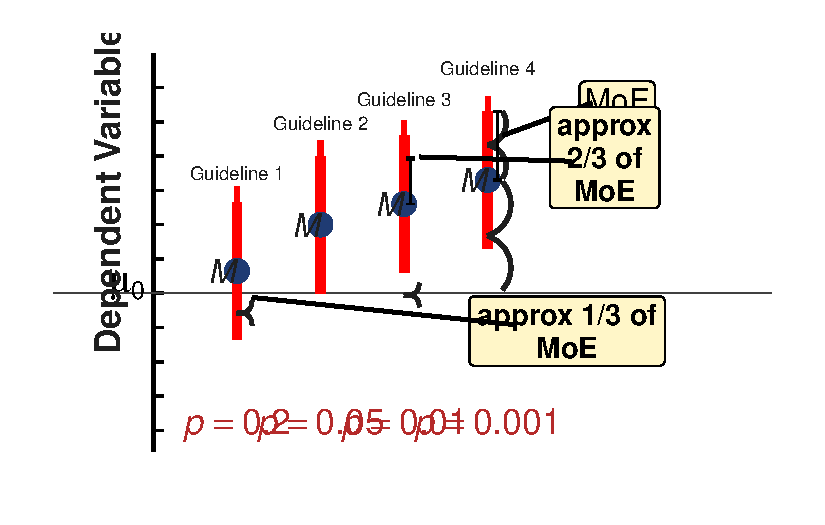
\includegraphics[keepaspectratio]{index_files/figure-pdf/unnamed-chunk-54-1.pdf}}

to approximate a rough estimate of the \(p\) value, rather than
replacing the precise calculation we'd require for an accurate \(p\)
value.

Naturally, you can apply these same guidelines when a CI is presented in
text format rather than displayed graphically. Suppose you encounter the
statement ``the decrease in mean response time was 32 ms {[}10, 54{]}.''
You want to estimate the \(p\) value for testing the null hypothesis of
zero change, meaning \(\mu_0 = 0\). First, observe that 0 falls outside
the CI, so we know \(p < .05\). Then visualize---either by sketching or
mentally---the CI and its position relative to zero. Comparing with
Figure 6.7, note that our CI falls between the two rightmost scenarios,
indicating \(p\) lies between .01 and .001, perhaps around .005.
Remember, we're content with approximate eyeballing---the goal is a
rough sense of the \(p\) value, not an exact calculation.

The figure above provides additional illustration of how the \(p\) value
varies depending on where a 95\% CI falls in relation to \(\mu_0\).
Imagine shifting \(M\) and the CI vertically, and approximating the
\(p\) value. The short dotted lines labeled with \(p\) values move
vertically with the CI, marking our four guidelines.

\begin{tcolorbox}[enhanced jigsaw, left=2mm, leftrule=.75mm, title={Exercise 6.9}, titlerule=0mm, toprule=.15mm, colframe=quarto-callout-note-color-frame, opacitybacktitle=0.6, bottomtitle=1mm, rightrule=.15mm, colbacktitle=quarto-callout-note-color!10!white, toptitle=1mm, arc=.35mm, colback=white, opacityback=0, bottomrule=.15mm, breakable, coltitle=black]

Open the \textbf{CI and p} page of ESCI intro chapters 3--8. Explore
freely. Use the large slider to shift the heavy blue 95\% CI vertically
in relation to the fixed \(\mu_0\) value. Try clicking on \textbf{Small
hints}. Compare with Figure 6.8.

\end{tcolorbox}

\begin{tcolorbox}[enhanced jigsaw, left=2mm, leftrule=.75mm, title={Exercise 6.10}, titlerule=0mm, toprule=.15mm, colframe=quarto-callout-note-color-frame, opacitybacktitle=0.6, bottomtitle=1mm, rightrule=.15mm, colbacktitle=quarto-callout-note-color!10!white, toptitle=1mm, arc=.35mm, colback=white, opacityback=0, bottomrule=.15mm, breakable, coltitle=black]

Create games or challenges to practice reading \(p\) values, given a
95\% CI and \(\mu_0\). For example, disable the \(p\) value (red 2) and
all hints, move \(M\), approximate \(p\), then enable the \(p\) value to
verify your accuracy. Aim for speed and competition.

\end{tcolorbox}

\textbf{6.11} For each of the 95\% CIs in Figure 6.9, estimate the \(p\)
value.

\textbf{6.12} You read that ``the increase in mean reading age was 2.3
months {[}−0.5, 5.1{]}.'' What is the approximate \(p\) value, for the
null hypothesis of zero increase?

If a 95\% CI falls so \(\mu_0\) is at a limit (i.e., exactly at one end
of the CI), then \(p = .05\). Suppose a 99\% CI falls so \(\mu_0\) is at
a limit, what do you think the \(p\) value would be?

\section{Type I and Type II Errors}\label{type-i-and-type-ii-errors}

Assuming that either \(H_0\) or \(H_1\) is true, two possible states of
reality exist: Either no effect exists and \(H_0\) is true, or an effect
exists and \(H_1\) is true. Additionally, we face two possible
decisions: Reject \(H_0\), or fail to reject \(H_0\). Consequently, four
possibilities emerge, as depicted in the four primary cells of Table
6.1.

Two cells represent desirable outcomes, where our decision would be
correct: In the upper left cell, no effect exists, \(H_0\) is true, and
we correctly fail to reject it. In the lower right cell, an effect
exists, \(H_1\) is true, and we correctly reject \(H_0\).

The remaining two cells represent errors, designated as \emph{Type I}
and \emph{Type II} errors:

\begin{tcolorbox}[enhanced jigsaw, colframe=quarto-callout-note-color-frame, left=2mm, leftrule=.75mm, rightrule=.15mm, opacityback=0, arc=.35mm, colback=white, bottomrule=.15mm, breakable, toprule=.15mm]
\begin{minipage}[t]{5.5mm}
\textcolor{quarto-callout-note-color}{\faInfo}
\end{minipage}%
\begin{minipage}[t]{\textwidth - 5.5mm}

\vspace{-3mm}\textbf{Type I Error}\vspace{3mm}

A \emph{Type I error} occurs when we reject \(H_0\) despite its truth,
as shown in the bottom left cell of Table 6.1.

\end{minipage}%
\end{tcolorbox}

A Type I error constitutes a \emph{false positive}. We declare ``There's
an effect!'', but unfortunately we're mistaken. If we reject the null
hypothesis that \(\mu = 50\) for College Alpha students when that value
is actually their true population mean HEAT score, then we commit a Type
I error.

\begin{tcolorbox}[enhanced jigsaw, colframe=quarto-callout-note-color-frame, left=2mm, leftrule=.75mm, rightrule=.15mm, opacityback=0, arc=.35mm, colback=white, bottomrule=.15mm, breakable, toprule=.15mm]
\begin{minipage}[t]{5.5mm}
\textcolor{quarto-callout-note-color}{\faInfo}
\end{minipage}%
\begin{minipage}[t]{\textwidth - 5.5mm}

\vspace{-3mm}\textbf{Type II Error}\vspace{3mm}

A \emph{Type II error} occurs when we fail to reject \(H_0\) despite its
falsity, as shown in the top right cell in Table 6.1.

\end{minipage}%
\end{tcolorbox}

A Type II error constitutes a \emph{false negative}, also termed a
\emph{miss}. An effect exists, yet we fail to detect it. If we don't
reject the null hypothesis that \(\mu = 50\) for College Alpha students
when their population mean HEAT score is actually \emph{not} 50, then we
commit a Type II error.

\textbf{6.21} If you select \(\alpha = .01\) and obtain \(p = .03\),
what decision do you make? Which cells in the table could you occupy?

\begin{itemize}
\tightlist
\item
  Describe and identify each of those cells.
\item
  Can you ever determine with certainty which single cell you occupy?
  Explain.
\item
  Can you ever be certain whether to feel satisfied or disappointed?
  Explain.
\end{itemize}

\textbf{6.22} Suppose you select \(\alpha = .05\) and obtain
\(p = .03\). Answer Exercise 6.21 for these values.

\textbf{6.23} What is \(\alpha\), what is \(p\), and how do they differ?

Next we address a crucial concept about \(\alpha\), and what it reveals
about Type I errors.

\section{\texorpdfstring{The Type I Error Rate, \(\alpha\), and What It
Means}{The Type I Error Rate, \textbackslash alpha, and What It Means}}\label{the-type-i-error-rate-alpha-and-what-it-means}

What is the probability of committing a Type I error when \(H_0\) holds
true? When \(H_0\) is true, we'll be unfortunate and obtain \(p < .05\)
in only 5\% of cases over the long run. This represents the fundamental
definition of the \(p\) value. Selecting \(\alpha = .05\), those 5\% of
instances occur when \(p < \alpha\) and we reject \(H_0\). Consequently,
\(\alpha\) represents the \emph{Type I error rate}---the probability of
making a Type I error when the null hypothesis is true.

\begin{tcolorbox}[enhanced jigsaw, colframe=quarto-callout-note-color-frame, left=2mm, leftrule=.75mm, rightrule=.15mm, opacityback=0, arc=.35mm, colback=white, bottomrule=.15mm, breakable, toprule=.15mm]
\begin{minipage}[t]{5.5mm}
\textcolor{quarto-callout-note-color}{\faInfo}
\end{minipage}%
\begin{minipage}[t]{\textwidth - 5.5mm}

\vspace{-3mm}\textbf{Type I Error Rate}\vspace{3mm}

The \emph{Type I error rate}, \(\alpha\), represents the probability of
rejecting \(H_0\) when it's actually true. This is also termed the
\emph{false positive rate}. (Refer to the bottom left cell in Table
6.1.)

\end{minipage}%
\end{tcolorbox}

\begin{equation}\phantomsection\label{eq-alpha}{
\alpha = \text{Probability (Reject } H_0\text{, WHEN } H_0 \text{ is true)}
}\end{equation}

It's essential to remember ``WHEN \(H_0\) is true'' (equivalent to ``IF
\(H_0\) is true'') for \(\alpha\), just as we must remember this
condition for \(p\) values. Both \(\alpha\) and a \(p\) value represent
probabilities that assume \(H_0\) holds true, and both can be
misinterpreted in identical ways. Recall the caution regarding
statements like ``The \(p\) value is the probability that \(H_0\) is
true.'' (Incorrect!) Similarly, we must guard against statements
claiming that \(\alpha\) represents the probability that \(H_0\) is
true, or the probability that no effect exists. (Both incorrect!)

Whenever you encounter \(\alpha\) or a \(p\) value, remind yourself
``assuming the null hypothesis is true.''

\textbf{6.24} Suppose you select \(\alpha = .05\). When the null
hypothesis holds true, what proportion of the NHST decisions you make
will constitute false positives? Can we ever determine with certainty
whether the null hypothesis is true?

\section{\texorpdfstring{The Type II Error Rate, \(\beta\), and What It
Means}{The Type II Error Rate, \textbackslash beta, and What It Means}}\label{the-type-ii-error-rate-beta-and-what-it-means}

I'll now define the \emph{Type II error rate}, which we denote as
\(\beta\).

\begin{tcolorbox}[enhanced jigsaw, colframe=quarto-callout-note-color-frame, left=2mm, leftrule=.75mm, rightrule=.15mm, opacityback=0, arc=.35mm, colback=white, bottomrule=.15mm, breakable, toprule=.15mm]
\begin{minipage}[t]{5.5mm}
\textcolor{quarto-callout-note-color}{\faInfo}
\end{minipage}%
\begin{minipage}[t]{\textwidth - 5.5mm}

\vspace{-3mm}\textbf{Type II Error Rate}\vspace{3mm}

The \emph{Type II error rate}, \(\beta\), represents the probability of
failing to reject \(H_0\) when it's actually false. This is also termed
the \emph{false negative rate}, or \emph{miss rate}. (Refer to the top
right cell in Table 6.1.)

\end{minipage}%
\end{tcolorbox}

\begin{equation}\phantomsection\label{eq-beta}{
\beta = \text{Probability (Don't reject } H_0\text{, WHEN } H_1 \text{ is true)}
}\end{equation}

To compute a \(p\) value and evaluate \(\alpha\), the Type I error rate,
we required a null hypothesis specifying a single value, such as
\(H_0: \mu = 0\). Similarly, to employ Equation~\ref{eq-beta} to
calculate \(\beta\), the Type II error rate, we need an alternative
hypothesis that specifies a single value. For our College Alpha example,
we might select:

\begin{itemize}
\tightlist
\item
  \(H_0: \mu = 50\) for the College Alpha student population.
\item
  \(H_1: \mu = 60\).
\end{itemize}

Why 60? We might select 60 because we know College Alpha maintains a
particularly robust environmental awareness program. Nevertheless, it's
somewhat artificial to assume that the population mean equals precisely
50 or precisely 60, but employing these hypotheses at least permits
calculation of both Type II and Type I error rates.

Using \(H_1: \mu = 60\), \(\beta\) calculated using
Equation~\ref{eq-beta} represents the probability we'll fail to detect
the difference from 50, assuming the College Alpha mean truly is 60.
Here we must note carefully that \(\beta\) is \emph{not} the probability
that \(H_1\) is true---rather, it's a probability that \emph{assumes}
\(H_1\) is true. Whenever you encounter \(\beta\) or any reference to
Type II errors, remind yourself ``assuming \(H_1\) is true,'' or
``assuming an effect of exactly that magnitude exists.''

\begin{Shaded}
\begin{Highlighting}[]
 \FunctionTok{library}\NormalTok{(ggplot2)}

\CommentTok{\# Set parameters}
\NormalTok{mu0 }\OtherTok{\textless{}{-}} \DecValTok{0}    \CommentTok{\# null hypothesis value (horizontal line position)}
\NormalTok{M }\OtherTok{\textless{}{-}} \SpecialCharTok{{-}}\FloatTok{2.5}   \CommentTok{\# sample mean position (center of the CI)}
\NormalTok{ci\_half\_width }\OtherTok{\textless{}{-}} \FloatTok{2.7} \CommentTok{\# margin of error (half{-}width of CI)}

\CommentTok{\# CI bounds}
\NormalTok{ci\_lower }\OtherTok{\textless{}{-}}\NormalTok{ M }\SpecialCharTok{{-}}\NormalTok{ ci\_half\_width}
\NormalTok{ci\_upper }\OtherTok{\textless{}{-}}\NormalTok{ M }\SpecialCharTok{+}\NormalTok{ ci\_half\_width}

\CommentTok{\# P{-}value positions (y{-}coordinates relative to mu0=0)}
\NormalTok{p\_positions }\OtherTok{\textless{}{-}} \FunctionTok{data.frame}\NormalTok{(}
  \AttributeTok{p\_value =} \FunctionTok{c}\NormalTok{(}\StringTok{".001"}\NormalTok{, }\StringTok{".01"}\NormalTok{, }\StringTok{".05"}\NormalTok{, }\StringTok{".20"}\NormalTok{),}
  \CommentTok{\# **ADJUSTMENT HERE:** .05 is now slightly above mu0 (0.1)}
  \AttributeTok{y =} \FunctionTok{c}\NormalTok{(}\FloatTok{2.5}\NormalTok{, }\FloatTok{1.5}\NormalTok{, }\FloatTok{0.1}\NormalTok{, }\SpecialCharTok{{-}}\FloatTok{0.7}\NormalTok{),}
  \AttributeTok{color =} \StringTok{"\#CC0000"}
\NormalTok{)}

\CommentTok{\# Create the plot}
\FunctionTok{ggplot}\NormalTok{() }\SpecialCharTok{+}
  
  \CommentTok{\# 1. Null Hypothesis Line (mu0) {-} Solid Black}
  \FunctionTok{geom\_hline}\NormalTok{(}\AttributeTok{yintercept =}\NormalTok{ mu0, }\AttributeTok{linewidth =} \FloatTok{1.5}\NormalTok{, }\AttributeTok{color =} \StringTok{"black"}\NormalTok{) }\SpecialCharTok{+} 
  
  \CommentTok{\# 2. Mean Line (M) {-} Thin Black line through the mean M}
  \FunctionTok{geom\_hline}\NormalTok{(}\AttributeTok{yintercept =}\NormalTok{ M, }\AttributeTok{linewidth =} \FloatTok{0.5}\NormalTok{, }\AttributeTok{color =} \StringTok{"black"}\NormalTok{) }\SpecialCharTok{+}
  
  \CommentTok{\# 3. Confidence Interval (CI) {-} Thick blue vertical line}
  \CommentTok{\# Reverting the linewidth back to a thicker value to match the screenshot better}
  \FunctionTok{geom\_segment}\NormalTok{(}\FunctionTok{aes}\NormalTok{(}\AttributeTok{x =} \DecValTok{0}\NormalTok{, }\AttributeTok{xend =} \DecValTok{0}\NormalTok{, }\AttributeTok{y =}\NormalTok{ ci\_lower, }\AttributeTok{yend =}\NormalTok{ ci\_upper),}
               \AttributeTok{linewidth =}\NormalTok{ .}\DecValTok{9}\NormalTok{, }\AttributeTok{color =} \StringTok{"\#264B86"}\NormalTok{) }\SpecialCharTok{+} 

  \CommentTok{\# 4. Mean Point {-} Solid filled circle}
  \FunctionTok{geom\_point}\NormalTok{(}\FunctionTok{aes}\NormalTok{(}\AttributeTok{x =} \DecValTok{0}\NormalTok{, }\AttributeTok{y =}\NormalTok{ M),}
             \AttributeTok{size =} \DecValTok{8}\NormalTok{, }\AttributeTok{color =} \StringTok{"\#264B86"}\NormalTok{, }\AttributeTok{fill =} \StringTok{"\#264B86"}\NormalTok{, }\AttributeTok{shape =} \DecValTok{21}\NormalTok{) }\SpecialCharTok{+} 

  \CommentTok{\# 5. Tick mark at mu0 on the CI (This represents the p=.05 *boundary*)}
  \FunctionTok{geom\_segment}\NormalTok{(}\FunctionTok{aes}\NormalTok{(}\AttributeTok{x =} \SpecialCharTok{{-}}\FloatTok{0.05}\NormalTok{, }\AttributeTok{xend =} \FloatTok{0.05}\NormalTok{, }\AttributeTok{y =}\NormalTok{ mu0, }\AttributeTok{yend =}\NormalTok{ mu0), }
               \AttributeTok{linewidth =} \DecValTok{1}\NormalTok{, }\AttributeTok{color =} \StringTok{"\#CC0000"}\NormalTok{) }\SpecialCharTok{+}
  
  \CommentTok{\# 6. Dotted p{-}value lines (only on the RIGHT side, dashed)}
  \CommentTok{\# This includes the now{-}adjusted .05 line which is above mu0}
  \FunctionTok{geom\_segment}\NormalTok{(}\AttributeTok{data =}\NormalTok{ p\_positions,}
               \FunctionTok{aes}\NormalTok{(}\AttributeTok{x =} \FloatTok{0.1}\NormalTok{, }\AttributeTok{xend =} \FloatTok{1.1}\NormalTok{, }\AttributeTok{y =}\NormalTok{ y, }\AttributeTok{yend =}\NormalTok{ y),}
               \AttributeTok{linetype =} \StringTok{"dashed"}\NormalTok{, }\AttributeTok{linewidth =} \FloatTok{1.1}\NormalTok{, }\AttributeTok{color =} \StringTok{"\#CC0000"}\NormalTok{) }\SpecialCharTok{+}
  
  \CommentTok{\# 7. P{-}value labels (Red text, right aligned)}
  \FunctionTok{geom\_text}\NormalTok{(}\AttributeTok{data =}\NormalTok{ p\_positions,}
            \FunctionTok{aes}\NormalTok{(}\AttributeTok{x =} \FloatTok{1.15}\NormalTok{, }\AttributeTok{y =}\NormalTok{ y, }\AttributeTok{label =}\NormalTok{ p\_value),}
            \AttributeTok{size =} \FloatTok{5.5}\NormalTok{, }\AttributeTok{color =} \StringTok{"\#CC0000"}\NormalTok{, }\AttributeTok{hjust =} \DecValTok{0}\NormalTok{, }\AttributeTok{fontface =} \StringTok{"plain"}\NormalTok{) }\SpecialCharTok{+}

  \CommentTok{\# 8. mu0 label (LaTeX formatting for Greek letter)}
  \FunctionTok{annotate}\NormalTok{(}\StringTok{"text"}\NormalTok{, }\AttributeTok{x =} \SpecialCharTok{{-}}\FloatTok{0.05}\NormalTok{, }\AttributeTok{y =}\NormalTok{ mu0 }\SpecialCharTok{+} \FloatTok{0.2}\NormalTok{, }\AttributeTok{label =} \StringTok{"mu[0]"}\NormalTok{,}
           \AttributeTok{size =} \DecValTok{7}\NormalTok{, }\AttributeTok{hjust =} \DecValTok{1}\NormalTok{, }\AttributeTok{parse =} \ConstantTok{TRUE}\NormalTok{) }\SpecialCharTok{+}
  
  \CommentTok{\# 9. M label (Italicized, close to the mean line)}
  \FunctionTok{annotate}\NormalTok{(}\StringTok{"text"}\NormalTok{, }\AttributeTok{x =} \SpecialCharTok{{-}}\FloatTok{0.05}\NormalTok{, }\AttributeTok{y =}\NormalTok{ M }\SpecialCharTok{{-}} \FloatTok{0.1}\NormalTok{, }\AttributeTok{label =} \StringTok{"italic(M)"}\NormalTok{,}
           \AttributeTok{size =} \DecValTok{7}\NormalTok{, }\AttributeTok{hjust =} \DecValTok{1}\NormalTok{, }\AttributeTok{parse =} \ConstantTok{TRUE}\NormalTok{) }\SpecialCharTok{+}
  
  \CommentTok{\# 10. Dependent Variable label (Rotated)}
  \FunctionTok{annotate}\NormalTok{(}\StringTok{"text"}\NormalTok{, }\AttributeTok{x =} \SpecialCharTok{{-}}\FloatTok{1.1}\NormalTok{, }\AttributeTok{y =} \DecValTok{0}\NormalTok{, }\AttributeTok{label =} \StringTok{"Dependent Variable"}\NormalTok{,}
           \AttributeTok{angle =} \DecValTok{90}\NormalTok{, }\AttributeTok{size =} \DecValTok{6}\NormalTok{, }\AttributeTok{fontface =} \StringTok{"plain"}\NormalTok{) }\SpecialCharTok{+}
  
  \CommentTok{\# 11. Axis lines (The main bounding box/axes from the original)}
  \FunctionTok{geom\_segment}\NormalTok{(}\FunctionTok{aes}\NormalTok{(}\AttributeTok{x =} \SpecialCharTok{{-}}\FloatTok{0.5}\NormalTok{, }\AttributeTok{xend =} \SpecialCharTok{{-}}\FloatTok{0.5}\NormalTok{, }\AttributeTok{y =} \SpecialCharTok{{-}}\FloatTok{4.5}\NormalTok{, }\AttributeTok{yend =} \FloatTok{3.5}\NormalTok{), }\AttributeTok{linewidth =} \FloatTok{0.8}\NormalTok{) }\SpecialCharTok{+} \CommentTok{\# Left Y{-}axis}
  
  \CommentTok{\# 12. Theme and Coordinates}
  \FunctionTok{coord\_cartesian}\NormalTok{(}\AttributeTok{xlim =} \FunctionTok{c}\NormalTok{(}\SpecialCharTok{{-}}\FloatTok{1.5}\NormalTok{, }\FloatTok{1.8}\NormalTok{), }\AttributeTok{ylim =} \FunctionTok{c}\NormalTok{(}\SpecialCharTok{{-}}\FloatTok{4.5}\NormalTok{, }\FloatTok{3.5}\NormalTok{), }\AttributeTok{expand =} \ConstantTok{FALSE}\NormalTok{) }\SpecialCharTok{+} \CommentTok{\# Set boundaries}
  \FunctionTok{theme\_minimal}\NormalTok{() }\SpecialCharTok{+}
  \FunctionTok{theme}\NormalTok{(}
    \AttributeTok{axis.title =} \FunctionTok{element\_blank}\NormalTok{(),}
    \AttributeTok{axis.text =} \FunctionTok{element\_blank}\NormalTok{(),}
    \AttributeTok{panel.grid =} \FunctionTok{element\_blank}\NormalTok{(),}
    \AttributeTok{panel.background =} \FunctionTok{element\_rect}\NormalTok{(}\AttributeTok{fill =} \StringTok{"white"}\NormalTok{, }\AttributeTok{color =} \ConstantTok{NA}\NormalTok{),}
    \AttributeTok{plot.background =} \FunctionTok{element\_rect}\NormalTok{(}\AttributeTok{fill =} \StringTok{"white"}\NormalTok{, }\AttributeTok{color =} \ConstantTok{NA}\NormalTok{),}
    \AttributeTok{plot.margin =} \FunctionTok{margin}\NormalTok{(}\DecValTok{20}\NormalTok{, }\DecValTok{10}\NormalTok{, }\DecValTok{10}\NormalTok{, }\DecValTok{20}\NormalTok{)}
\NormalTok{  )}
\end{Highlighting}
\end{Shaded}

\pandocbounded{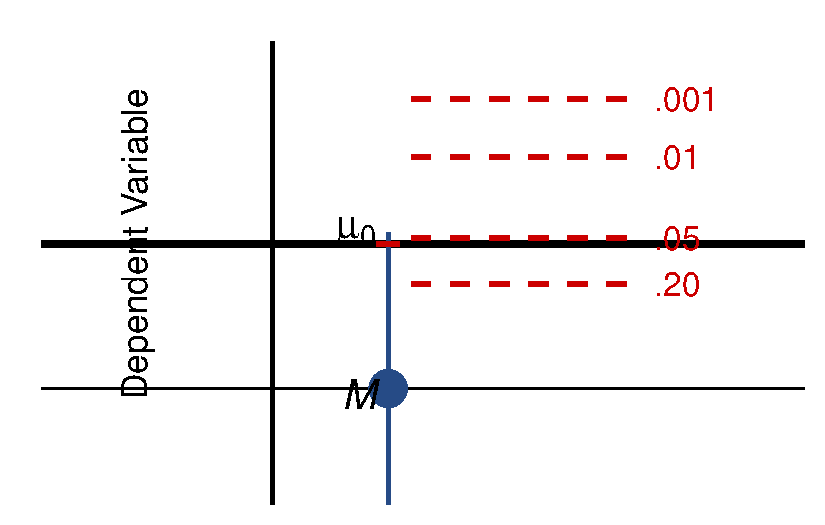
\includegraphics[keepaspectratio]{index_files/figure-pdf/unnamed-chunk-55-1.pdf}}

\section{The Independent Groups
Design}\label{the-independent-groups-design}

Researchers frequently seek to examine differences between two
conditions---for instance, comparing note-taking using pen versus
laptop. This chapter explores the design that contrasts conditions by
employing separate, independent groups of participants. Subsequently, in
Chapter 8, we'll examine an alternative approach: the paired design,
wherein a single group of participants provides data for both
conditions.

This chapter begins with fundamental concepts for independent groups:
The estimation framework, which emphasizes the difference between two
means---our effect size---along with its CI. I'll then present an
alternative method for expressing this effect size, utilizing a
standardized effect size measure termed Cohen's \(d\). Cohen's \(d\)
represents a remarkably valuable measure that enables us to compare
findings across diverse types of studies. Finally, I'll examine a second
analytical approach, grounded in NHST and \(p\) values. The chapter
addresses these essential topics:

\begin{itemize}
\tightlist
\item
  The independent groups design
\item
  The CI on the difference between two means
\item
  Cohen's \(d\), a standardized effect size measure
\item
  Interpreting \(d\) and the CI on \(d\)
\item
  Applying \(p\) values and NHST with independent groups
\item
  The dance of the \(p\) values, a revealing illustration of
  variability, and Red Flag 5
\end{itemize}

\section{The Independent Groups
Design}\label{the-independent-groups-design-1}

In the independent groups design, each participant undergoes testing in
only one of the two conditions under comparison.

To contrast note-taking with pen versus laptop, Mueller and Oppenheimer
(2014) employed two independent groups, randomly assigning students to
the two conditions. This exemplifies the \emph{independent groups
design}, wherein the performance data collected with pen are independent
of the data collected with laptop because they originate from distinct
groups of students. This constitutes an experiment, which supports a
conclusion that any observed difference was most likely caused by the
Pen--Laptop independent variable.

The study revealed that students learned more effectively after taking
notes in longhand compared to typing notes. The researchers hypothesized
that writing might encourage expression of concepts in students' own
words, whereas typing might promote relatively mindless transcription
that resulted in comparatively poor learning. To investigate this
hypothesis, the researchers developed a transcription score: the
percentage of notes representing verbatim transcription from the
lecture. Following Chapter 2, transcription score serves as the
dependent variable I'll examine here.

The initial step involves examining the data. Figure 7.1 displays
individual data points, which demonstrate substantial variation within
both groups. As we compute descriptive and inferential statistics,
continuously bear in mind the underlying individual data. Avoid allowing
a pattern of means to mislead you---individuals may not conform to the
overall trend.

\begin{Shaded}
\begin{Highlighting}[]
\CommentTok{\#| label: fig{-}transcription{-}data}
\CommentTok{\#| fig{-}cap: "The Pen–Laptop transcription data for independent groups. Open dots are data for individual students. Group means $M\_1$ and $M\_2$ and 95\% CIs, are displayed."}
\CommentTok{\#| fig{-}width: 6}
\CommentTok{\#| fig{-}height: 6}
\CommentTok{\#| cache: false}
\CommentTok{\#| dev: "png"}

\FunctionTok{library}\NormalTok{(ggplot2)}
\FunctionTok{library}\NormalTok{(dplyr)}

\CommentTok{\# Simulate data based on the figure}
\FunctionTok{set.seed}\NormalTok{(}\DecValTok{123}\NormalTok{)}

\CommentTok{\# Pen group data (approximately matching the scatter in the figure)}
\NormalTok{pen\_data }\OtherTok{\textless{}{-}} \FunctionTok{c}\NormalTok{(}\DecValTok{20}\NormalTok{, }\DecValTok{18}\NormalTok{, }\FloatTok{17.5}\NormalTok{, }\FloatTok{14.5}\NormalTok{, }\DecValTok{13}\NormalTok{, }\FloatTok{12.5}\NormalTok{, }\DecValTok{12}\NormalTok{, }\FloatTok{11.5}\NormalTok{, }\DecValTok{11}\NormalTok{, }\FloatTok{10.5}\NormalTok{, }\DecValTok{10}\NormalTok{, }\FloatTok{9.5}\NormalTok{, }\DecValTok{9}\NormalTok{, }
              \FloatTok{8.5}\NormalTok{, }\DecValTok{8}\NormalTok{, }\FloatTok{7.5}\NormalTok{, }\DecValTok{7}\NormalTok{, }\FloatTok{6.5}\NormalTok{, }\DecValTok{5}\NormalTok{, }\DecValTok{5}\NormalTok{, }\DecValTok{3}\NormalTok{, }\FloatTok{2.5}\NormalTok{, }\DecValTok{2}\NormalTok{, }\DecValTok{1}\NormalTok{, }\FloatTok{0.5}\NormalTok{)}

\CommentTok{\# Laptop group data (approximately matching the scatter in the figure)}
\NormalTok{laptop\_data }\OtherTok{\textless{}{-}} \FunctionTok{c}\NormalTok{(}\DecValTok{35}\NormalTok{, }\FloatTok{30.5}\NormalTok{, }\FloatTok{26.5}\NormalTok{, }\FloatTok{21.5}\NormalTok{, }\DecValTok{21}\NormalTok{, }\DecValTok{19}\NormalTok{, }\FloatTok{18.5}\NormalTok{, }\DecValTok{18}\NormalTok{, }\FloatTok{17.5}\NormalTok{, }\DecValTok{17}\NormalTok{, }\FloatTok{16.5}\NormalTok{, }\DecValTok{16}\NormalTok{, }
                 \FloatTok{15.5}\NormalTok{, }\DecValTok{14}\NormalTok{, }\FloatTok{13.5}\NormalTok{, }\DecValTok{13}\NormalTok{, }\DecValTok{13}\NormalTok{, }\FloatTok{12.5}\NormalTok{, }\DecValTok{12}\NormalTok{, }\FloatTok{11.5}\NormalTok{, }\FloatTok{10.5}\NormalTok{, }\DecValTok{10}\NormalTok{, }\FloatTok{9.5}\NormalTok{, }\DecValTok{9}\NormalTok{, }
                 \FloatTok{8.5}\NormalTok{, }\DecValTok{8}\NormalTok{, }\DecValTok{5}\NormalTok{, }\FloatTok{4.5}\NormalTok{, }\FloatTok{1.5}\NormalTok{)}

\CommentTok{\# Combine into a data frame}
\NormalTok{data }\OtherTok{\textless{}{-}} \FunctionTok{data.frame}\NormalTok{(}
  \AttributeTok{Transcription =} \FunctionTok{c}\NormalTok{(pen\_data, laptop\_data),}
  \AttributeTok{Condition =} \FunctionTok{factor}\NormalTok{(}\FunctionTok{rep}\NormalTok{(}\FunctionTok{c}\NormalTok{(}\StringTok{"Pen"}\NormalTok{, }\StringTok{"Laptop"}\NormalTok{), }\FunctionTok{c}\NormalTok{(}\FunctionTok{length}\NormalTok{(pen\_data), }\FunctionTok{length}\NormalTok{(laptop\_data))),}
                     \AttributeTok{levels =} \FunctionTok{c}\NormalTok{(}\StringTok{"Pen"}\NormalTok{, }\StringTok{"Laptop"}\NormalTok{))}
\NormalTok{)}

\CommentTok{\# Calculate means and 95\% CIs}
\NormalTok{summary\_stats }\OtherTok{\textless{}{-}}\NormalTok{ data }\SpecialCharTok{\%\textgreater{}\%}
  \FunctionTok{group\_by}\NormalTok{(Condition) }\SpecialCharTok{\%\textgreater{}\%}
  \FunctionTok{summarise}\NormalTok{(}
    \AttributeTok{M =} \FunctionTok{mean}\NormalTok{(Transcription),}
    \AttributeTok{SE =} \FunctionTok{sd}\NormalTok{(Transcription) }\SpecialCharTok{/} \FunctionTok{sqrt}\NormalTok{(}\FunctionTok{n}\NormalTok{()),}
    \AttributeTok{CI\_lower =}\NormalTok{ M }\SpecialCharTok{{-}} \FloatTok{1.96} \SpecialCharTok{*}\NormalTok{ SE,}
    \AttributeTok{CI\_upper =}\NormalTok{ M }\SpecialCharTok{+} \FloatTok{1.96} \SpecialCharTok{*}\NormalTok{ SE,}
    \AttributeTok{.groups =} \StringTok{\textquotesingle{}drop\textquotesingle{}}
\NormalTok{  )}

\CommentTok{\# Create the plot}
\FunctionTok{ggplot}\NormalTok{(data, }\FunctionTok{aes}\NormalTok{(}\AttributeTok{x =}\NormalTok{ Condition, }\AttributeTok{y =}\NormalTok{ Transcription)) }\SpecialCharTok{+}
  \CommentTok{\# Add individual data points (open circles)}
  \FunctionTok{geom\_point}\NormalTok{(}
    \AttributeTok{shape =} \DecValTok{1}\NormalTok{, }
    \AttributeTok{size =} \FloatTok{2.5}\NormalTok{, }
    \AttributeTok{color =} \StringTok{"red"}\NormalTok{, }
    \AttributeTok{position =} \FunctionTok{position\_jitter}\NormalTok{(}\AttributeTok{width =} \FloatTok{0.08}\NormalTok{, }\AttributeTok{height =} \DecValTok{0}\NormalTok{, }\AttributeTok{seed =} \DecValTok{123}\NormalTok{),}
    \AttributeTok{alpha =} \DecValTok{1}
\NormalTok{  ) }\SpecialCharTok{+}
  
  \CommentTok{\# Add 95\% CI error bars}
  \FunctionTok{geom\_errorbar}\NormalTok{(}
    \AttributeTok{data =}\NormalTok{ summary\_stats,}
    \FunctionTok{aes}\NormalTok{(}\AttributeTok{x =}\NormalTok{ Condition, }\AttributeTok{y =}\NormalTok{ M, }\AttributeTok{ymin =}\NormalTok{ CI\_lower, }\AttributeTok{ymax =}\NormalTok{ CI\_upper),}
    \AttributeTok{width =} \DecValTok{0}\NormalTok{, }
    \AttributeTok{linewidth =} \FloatTok{1.2}\NormalTok{, }
    \AttributeTok{color =} \StringTok{"black"}\NormalTok{,}
    \AttributeTok{inherit.aes =} \ConstantTok{FALSE}
\NormalTok{  ) }\SpecialCharTok{+}
  
  \CommentTok{\# Add mean points (filled circles)}
  \FunctionTok{geom\_point}\NormalTok{(}
    \AttributeTok{data =}\NormalTok{ summary\_stats,}
    \FunctionTok{aes}\NormalTok{(}\AttributeTok{x =}\NormalTok{ Condition, }\AttributeTok{y =}\NormalTok{ M),}
    \AttributeTok{size =} \DecValTok{4}\NormalTok{, }
    \AttributeTok{color =} \StringTok{"black"}\NormalTok{, }
    \AttributeTok{shape =} \DecValTok{16}\NormalTok{,}
    \AttributeTok{inherit.aes =} \ConstantTok{FALSE}
\NormalTok{  ) }\SpecialCharTok{+}
  
  \CommentTok{\# Add mean labels (M1, M2)}
  \FunctionTok{geom\_text}\NormalTok{(}
    \AttributeTok{data =}\NormalTok{ summary\_stats,}
    \FunctionTok{aes}\NormalTok{(}\AttributeTok{x =}\NormalTok{ Condition, }\AttributeTok{y =}\NormalTok{ M, }
        \AttributeTok{label =} \FunctionTok{ifelse}\NormalTok{(Condition }\SpecialCharTok{==} \StringTok{"Pen"}\NormalTok{, }\StringTok{"italic(M)[1]"}\NormalTok{, }\StringTok{"italic(M)[2]"}\NormalTok{)),}
    \AttributeTok{parse =} \ConstantTok{TRUE}\NormalTok{, }
    \AttributeTok{hjust =} \SpecialCharTok{{-}}\FloatTok{0.6}\NormalTok{, }
    \AttributeTok{size =} \DecValTok{5}\NormalTok{,}
    \AttributeTok{inherit.aes =} \ConstantTok{FALSE}
\NormalTok{  ) }\SpecialCharTok{+}
  
  \CommentTok{\# Customize axes}
  \FunctionTok{scale\_y\_continuous}\NormalTok{(}\AttributeTok{limits =} \FunctionTok{c}\NormalTok{(}\DecValTok{0}\NormalTok{, }\DecValTok{36}\NormalTok{), }\AttributeTok{breaks =} \FunctionTok{seq}\NormalTok{(}\DecValTok{0}\NormalTok{, }\DecValTok{35}\NormalTok{, }\DecValTok{5}\NormalTok{)) }\SpecialCharTok{+}
  \FunctionTok{scale\_x\_discrete}\NormalTok{(}\AttributeTok{expand =} \FunctionTok{expansion}\NormalTok{(}\AttributeTok{add =} \FloatTok{0.4}\NormalTok{)) }\SpecialCharTok{+}
  
  \CommentTok{\# Labels}
  \FunctionTok{labs}\NormalTok{(}\AttributeTok{y =} \StringTok{"Transcription \%"}\NormalTok{, }\AttributeTok{x =} \ConstantTok{NULL}\NormalTok{) }\SpecialCharTok{+}
  
  \CommentTok{\# Theme}
  \FunctionTok{theme\_classic}\NormalTok{() }\SpecialCharTok{+}
  \FunctionTok{theme}\NormalTok{(}
    \AttributeTok{axis.text =} \FunctionTok{element\_text}\NormalTok{(}\AttributeTok{size =} \DecValTok{11}\NormalTok{),}
    \AttributeTok{axis.title =} \FunctionTok{element\_text}\NormalTok{(}\AttributeTok{size =} \DecValTok{12}\NormalTok{),}
    \AttributeTok{axis.line =} \FunctionTok{element\_line}\NormalTok{(}\AttributeTok{linewidth =} \FloatTok{0.8}\NormalTok{),}
    \AttributeTok{axis.ticks =} \FunctionTok{element\_line}\NormalTok{(}\AttributeTok{linewidth =} \FloatTok{0.7}\NormalTok{)}
\NormalTok{  )}
\end{Highlighting}
\end{Shaded}

\pandocbounded{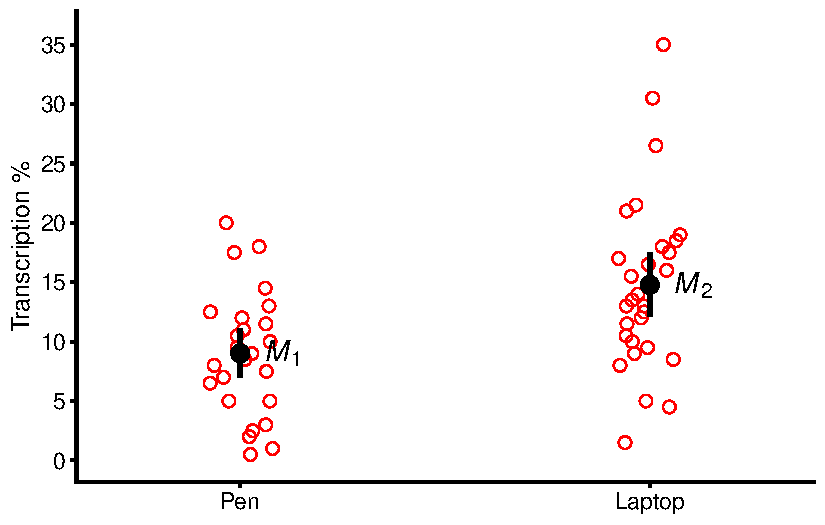
\includegraphics[keepaspectratio]{index_files/figure-pdf/unnamed-chunk-56-1.pdf}}

\begin{longtable}[]{@{}lllll@{}}
\toprule\noalign{}
& Pen & & Laptop & \\
\midrule\noalign{}
\endhead
\bottomrule\noalign{}
\endlastfoot
\(N\) & \(N_1\) & 34 & \(N_2\) & 31 \\
Mean & \(M_1\) & 8.81 & \(M_2\) & 14.52 \\
SD & \(s_1\) & 4.75 & \(s_2\) & 7.29 \\
MoE & \(\text{MoE}_1\) & 1.66 & \(\text{MoE}_2\) & 2.67 \\
\end{longtable}

\textbf{7.1} Determine how Figures 7.1 and 7.2 depict each value
presented in Table 7.1. When approximating from the figures, do the
values appear reasonable?

Now for the calculations. The difference itself is straightforward:

\[
(M_2 - M_1) = 14.52 - 8.81 = 5.71
\]

Our fundamental CI formula from Chapter 5 establishes that a CI is
\([M - \text{MoE}, M + \text{MoE}]\). To compute the 95\% CI on a single
mean when \(\sigma\) is unknown, we employed:

\begin{equation}\phantomsection\label{eq-moe-single}{
\text{MoE} = t_{.95}(df) \times s \times \left(\frac{1}{\sqrt{N}}\right)
}\end{equation}

{ \(t\) component, which makes it a 95\% CI \textbar{} Variability
component \textbar{} Sample size component }

For the CI we require on our effect size, the difference, we need an
analogous formula. I've identified three components in
Equation~\ref{eq-moe-single} to facilitate explaining the CI on the
difference. Let's examine the three components.

\textbf{The \(t\) component for the difference} is \(t_{.95}(df)\),
where each group contributes to \(df\), and consequently \(df\) for the
difference between independent means is:

\begin{equation}\phantomsection\label{eq-df-independent}{
df = (N_1 - 1) + (N_2 - 1) = (N_1 + N_2 - 2)
}\end{equation}

\textbf{The variability component for the difference} must reflect
variability in both the Pen and Laptop populations, as estimated by our
\(s_1\) and \(s_2\), which represent the SDs of the two groups. Table
7.1 indicates their values are 4.75 and 7.29 respectively. Our
statistical model assumes that the two populations---the populations of
Pen and Laptop scores---possess the same SD, which I'll designate
\(\sigma\). Equivalently, I can state the two populations have the same
variance, \(\sigma^2\). This represents the third assumption of our
model, the \emph{homogeneity of variance} assumption. Frequently, though
not invariably, it's reasonable to make this assumption, and we'll
employ it here.

The subsequent step is to combine, or \emph{pool}, \(s_1\) and \(s_2\)
to calculate \(s_p\), the pooled SD, which constitutes our best estimate
of \(\sigma\). Here's the formula:

\begin{equation}\phantomsection\label{eq-pooled-sd}{
s_p = \sqrt{\frac{(N_1 - 1)s_1^2 + (N_2 - 1)s_2^2}{N_1 + N_2 - 2}}
}\end{equation}

The group standard deviations, \(s_1\) and \(s_2\), measure the spread
\emph{within} each group. The pooled standard deviation, \(s_p\),
represents a type of weighted average of \(s_1\) and \(s_2\), and
therefore \(s_p\) is termed the \emph{pooled SD within groups}. It's the
variability component we need for calculating the CI.

\textbf{The sample size component for the difference} is
\(\sqrt{\frac{1}{N_1} + \frac{1}{N_2}}\), which reflects the sizes of
both our Pen and Laptop samples, as we'd anticipate.

\bookmarksetup{startatroot}

\chapter{Chapter 12: Regression}\label{chapter-12-regression}

In the previous chapter, we examined \textbf{scatterplots} and
\textbf{correlation coefficients} as tools for describing relationships
between two quantitative variables. A correlation coefficient
conveniently summarizes both the \emph{strength} and \emph{direction} of
a linear association. However, a correlation does not tell us \emph{how
much} one variable changes when the other changes. For that, we use
\textbf{regression analysis}.

\section{What Is a Regression Line?}\label{what-is-a-regression-line}

A \textbf{regression line} is a straight line that models how a
\textbf{response variable} (\(y\)) changes as an \textbf{explanatory
variable} (\(x\)) changes. While a correlation measures association, a
regression line allows for \textbf{prediction}.

For example, suppose we are interested in the relationship between
\textbf{education} and \textbf{earnings}. The correlation coefficient
tells us whether the two are positively or negatively associated, and
how strongly. But if we want to know \emph{how much} additional income
is expected from one extra year of education, we use regression. A
regression line lets us estimate the \textbf{expected change in
earnings} for a one-unit increase in education.

\section{The Idea of a ``Best-Fitting''
Line}\label{the-idea-of-a-best-fitting-line}

A regression line provides the best-fitting straight line through a
cloud of points in a scatterplot. It summarizes the linear relationship
between two variables.

Consider a plot showing the relationship between a state's
\textbf{median household income} and the \textbf{percentage of voters
supporting Donald Trump}. Some states (like Wyoming) may be far above or
below the line. The regression line does not pass through every point
but instead \emph{minimizes the overall distance} between the observed
data and the line itself.

This method is known as \textbf{Ordinary Least Squares (OLS)}
regression. OLS determines the line that minimizes the \textbf{sum of
squared vertical deviations} between the observed values (\(y_i\)) and
the predicted values (\(\hat{y}_i\)):

\[
\sum (y_i - \hat{y}_i)^2
\]

Each vertical deviation (often shown as a red arrow) represents the
\textbf{residual} or \textbf{error} for that observation. The regression
algorithm adjusts the line so that the total of these squared residuals
is as small as possible.

\section{The Regression Equation}\label{the-regression-equation}

You may recall the general equation of a line from algebra:

\[
y = mx + b
\]

In regression notation, this becomes:

\[
\hat{y} = a + bx
\]

where:

\begin{itemize}
\tightlist
\item
  \(\hat{y}\) = the \emph{predicted} value of \(y\)\\
\item
  \(a\) = the \textbf{intercept}, or the predicted value of \(y\) when
  \(x = 0\)\\
\item
  \(b\) = the \textbf{slope}, or the expected change in \(y\) for a
  one-unit increase in \(x\)
\end{itemize}

\subsection{Interpretation of
Coefficients}\label{interpretation-of-coefficients}

\begin{itemize}
\tightlist
\item
  The \textbf{intercept} (\(a\)) is the point at which the line crosses
  the \(y\)-axis.\\
\item
  The \textbf{slope} (\(b\)) represents the \emph{rate of change}: for
  each one-unit increase in \(x\), \(y\) is predicted to change by \(b\)
  units.\\
\item
  If \(b = 0\), the line is horizontal, indicating no linear
  relationship between \(x\) and \(y\).
\end{itemize}

\section{Example: Income and Trump Vote
Share}\label{example-income-and-trump-vote-share}

Suppose the estimated regression equation is:

\[
\hat{y} = 85.8 - 0.66x
\]

where:

\begin{itemize}
\tightlist
\item
  \(y\) = percent voting for Trump\\
\item
  \(x\) = median household income (in thousands of dollars)
\end{itemize}

Here, the \textbf{slope} (\(b = -0.66\)) tells us that for every
additional \$1,000 in median household income, the predicted Trump vote
share decreases by 0.66 percentage points. The \textbf{intercept}
(\(a = 85.8\)) is the predicted vote share when median income equals
zero --- mathematically necessary but not substantively meaningful.

\subsection{Example Prediction}\label{example-prediction}

For Wisconsin, the median household income in 2015 was \$55,402, or
\(x = 55.402\) (in thousands). Substituting into the regression
equation:

\[
\hat{y} = 85.8 - 0.66(55.402) = 49.23
\]

Thus, the model predicts that \textbf{49.23\% of Wisconsin voters} would
support Trump.\\
The actual percentage was slightly lower, showing that while regression
provides a useful \emph{prediction}, it does not perfectly describe
every case.

\begin{quote}
\textbf{Note:} Always interpret regression relationships as
\emph{associations}, not certainties. Use language such as ``is
associated with,'' ``tends to,'' or ``is predicted to,'' rather than
deterministic statements like ``causes'' or ``declines by exactly.''
\end{quote}

\begin{center}\rule{0.5\linewidth}{0.5pt}\end{center}

\section{Interpreting the Intercept}\label{interpreting-the-intercept}

The intercept \(a\) represents the predicted value of \(y\) when
\(x = 0\). Sometimes this is meaningful---for example, predicting flight
delays when outsourcing equals zero percent.\\
In other cases, such as predicting adult smoking rates when age = 0, it
is not substantively interpretable. Always interpret the intercept only
within the range of observed data.

\begin{center}\rule{0.5\linewidth}{0.5pt}\end{center}

\section{Example: Airline Outsourcing and Flight
Delays}\label{example-airline-outsourcing-and-flight-delays}

Consider the regression equation:

\[
\hat{y} = 21.8 - 0.126x
\]

where:

\begin{itemize}
\tightlist
\item
  \(y\) = percent of flights delayed\\
\item
  \(x\) = percent of flights outsourced
\end{itemize}

Here, the intercept (21.8) indicates that when outsourcing equals zero,
the predicted delay rate is 21.8\%. The slope (\(-0.126\)) means that
for each one-percentage-point increase in outsourcing, flight delays are
predicted to decrease by 0.126 percentage points.

\subsection{Example Prediction}\label{example-prediction-1}

If an airline outsources 75\% of its flights:

\[
\hat{y} = 21.8 - 0.126(75) = 12.35
\]

The predicted delay rate is \textbf{12.35\%}, consistent with the
direction and magnitude shown by the regression line.

\begin{center}\rule{0.5\linewidth}{0.5pt}\end{center}

\section{\texorpdfstring{The Coefficient of Determination:
\(R^2\)}{The Coefficient of Determination: R\^{}2}}\label{the-coefficient-of-determination-r2}

The \textbf{\(R^2\) statistic} measures how well the regression line
explains the variation in \(y\). Formally, \(R^2\) is the
\textbf{fraction of variance in \(y\) explained by the regression}:

\[
R^2 = \frac{\text{Explained Variation in } y}{\text{Total Variation in } y}
\]

The correlation coefficient \(r\) ranges between --1 and 1; squaring it
produces \(R^2\), which ranges from 0 to 1.

\begin{itemize}
\tightlist
\item
  \(R^2 = 1\): all points fall exactly on the line (perfect fit)\\
\item
  \(R^2 = 0\): no linear relationship; \(x\) explains none of the
  variation in \(y\)
\end{itemize}

In the airline example, the correlation coefficient is \(r = -0.489\).
Thus:

\[
R^2 = (-0.489)^2 = 0.238
\]

This means that \textbf{approximately 24\% of the variation} in flight
delay rates is explained by variation in outsourcing levels.

\begin{center}\rule{0.5\linewidth}{0.5pt}\end{center}

\section{\texorpdfstring{Common Misinterpretations of
\(R^2\)}{Common Misinterpretations of R\^{}2}}\label{common-misinterpretations-of-r2}

It is crucial to interpret \(R^2\) correctly.

A common mistake is to say:

\begin{quote}
``Outsourcing accounts for 24\% of flight delays.''
\end{quote}

The correct interpretation is:

\begin{quote}
``Variation in outsourcing explains 24\% of the \emph{variation} in
flight delays.''
\end{quote}

To clarify, consider an analogy with \textbf{pizza prices}:

\begin{itemize}
\tightlist
\item
  A plain cheese pizza costs \$8.\\
\item
  Each topping adds \$0.20.
\end{itemize}

Toppings do not explain \emph{100\% of the price} of a pizza---because
even with zero toppings, the base price is \$8.\\
However, \textbf{variation} in the number of toppings fully explains the
\textbf{variation} in total cost.

In regression terms, this means:\\
Variation in \(x\) (toppings) explains 100\% of the variation in \(y\)
(price), just as variation in outsourcing explains 24\% of the variation
in delays.

\begin{center}\rule{0.5\linewidth}{0.5pt}\end{center}

\begin{Shaded}
\begin{Highlighting}[]
\CommentTok{\#| label: fig{-}regression{-}ci{-}bands}
\CommentTok{\#| fig{-}cap: "Regression line with 90\% confidence intervals for fitted and predicted values."}
\CommentTok{\#| fig{-}width: 11}
\CommentTok{\#| fig{-}height: 7.2}
\CommentTok{\#| dpi: 200}
\CommentTok{\#| out{-}width: 100\%}
\CommentTok{\#| warning: false}
\CommentTok{\#| message: false}

\FunctionTok{suppressPackageStartupMessages}\NormalTok{(\{}
  \FunctionTok{library}\NormalTok{(ggplot2)}
  \FunctionTok{library}\NormalTok{(dplyr)}
\NormalTok{\})}

\CommentTok{\# Generate example data}
\FunctionTok{set.seed}\NormalTok{(}\DecValTok{123}\NormalTok{)}
\NormalTok{n }\OtherTok{\textless{}{-}} \DecValTok{100}
\NormalTok{waist\_cm }\OtherTok{\textless{}{-}} \FunctionTok{runif}\NormalTok{(n, }\DecValTok{55}\NormalTok{, }\DecValTok{125}\NormalTok{)}
\NormalTok{sqrt\_vat }\OtherTok{\textless{}{-}} \SpecialCharTok{{-}}\DecValTok{10} \SpecialCharTok{+} \FloatTok{0.5} \SpecialCharTok{*}\NormalTok{ waist\_cm }\SpecialCharTok{+} \FunctionTok{rnorm}\NormalTok{(n, }\DecValTok{0}\NormalTok{, }\DecValTok{5}\NormalTok{)}
\NormalTok{df }\OtherTok{\textless{}{-}} \FunctionTok{data.frame}\NormalTok{(waist\_cm, sqrt\_vat)}

\CommentTok{\# Fit model}
\NormalTok{fit }\OtherTok{\textless{}{-}} \FunctionTok{lm}\NormalTok{(sqrt\_vat }\SpecialCharTok{\textasciitilde{}}\NormalTok{ waist\_cm, }\AttributeTok{data =}\NormalTok{ df)}

\CommentTok{\# Get predictions with confidence and prediction intervals}
\NormalTok{pred\_data }\OtherTok{\textless{}{-}} \FunctionTok{data.frame}\NormalTok{(}\AttributeTok{waist\_cm =} \FunctionTok{seq}\NormalTok{(}\FunctionTok{min}\NormalTok{(df}\SpecialCharTok{$}\NormalTok{waist\_cm), }\FunctionTok{max}\NormalTok{(df}\SpecialCharTok{$}\NormalTok{waist\_cm), }\AttributeTok{length.out =} \DecValTok{200}\NormalTok{))}
\NormalTok{ci\_fitted }\OtherTok{\textless{}{-}} \FunctionTok{predict}\NormalTok{(fit, }\AttributeTok{newdata =}\NormalTok{ pred\_data, }\AttributeTok{interval =} \StringTok{"confidence"}\NormalTok{, }\AttributeTok{level =} \FloatTok{0.90}\NormalTok{)}
\NormalTok{ci\_predicted }\OtherTok{\textless{}{-}} \FunctionTok{predict}\NormalTok{(fit, }\AttributeTok{newdata =}\NormalTok{ pred\_data, }\AttributeTok{interval =} \StringTok{"prediction"}\NormalTok{, }\AttributeTok{level =} \FloatTok{0.90}\NormalTok{)}

\NormalTok{pred\_data }\OtherTok{\textless{}{-}}\NormalTok{ pred\_data }\SpecialCharTok{\%\textgreater{}\%}
  \FunctionTok{mutate}\NormalTok{(}
    \AttributeTok{fit =}\NormalTok{ ci\_fitted[, }\StringTok{"fit"}\NormalTok{],}
    \AttributeTok{ci\_lwr =}\NormalTok{ ci\_fitted[, }\StringTok{"lwr"}\NormalTok{],}
    \AttributeTok{ci\_upr =}\NormalTok{ ci\_fitted[, }\StringTok{"upr"}\NormalTok{],}
    \AttributeTok{pred\_lwr =}\NormalTok{ ci\_predicted[, }\StringTok{"lwr"}\NormalTok{],}
    \AttributeTok{pred\_upr =}\NormalTok{ ci\_predicted[, }\StringTok{"upr"}\NormalTok{]}
\NormalTok{  )}

\CommentTok{\# Select 3 points to show CI bars}
\NormalTok{show\_points }\OtherTok{\textless{}{-}} \FunctionTok{c}\NormalTok{(}\DecValTok{20}\NormalTok{, }\DecValTok{50}\NormalTok{, }\DecValTok{80}\NormalTok{)}
\NormalTok{ci\_bars }\OtherTok{\textless{}{-}}\NormalTok{ pred\_data[show\_points, ]}

\CommentTok{\# Create plot}
\FunctionTok{ggplot}\NormalTok{(df, }\FunctionTok{aes}\NormalTok{(}\AttributeTok{x =}\NormalTok{ waist\_cm, }\AttributeTok{y =}\NormalTok{ sqrt\_vat)) }\SpecialCharTok{+}
  \CommentTok{\# Regression line}
  \FunctionTok{geom\_line}\NormalTok{(}\AttributeTok{data =}\NormalTok{ pred\_data, }\FunctionTok{aes}\NormalTok{(}\AttributeTok{y =}\NormalTok{ fit), }\AttributeTok{color =} \StringTok{"black"}\NormalTok{, }\AttributeTok{linewidth =} \FloatTok{1.2}\NormalTok{) }\SpecialCharTok{+}
  
  \CommentTok{\# Sexy dashed residual lines connecting points to regression line}
  \FunctionTok{geom\_segment}\NormalTok{(}\FunctionTok{aes}\NormalTok{(}\AttributeTok{x =}\NormalTok{ waist\_cm, }\AttributeTok{xend =}\NormalTok{ waist\_cm, }
                   \AttributeTok{y =}\NormalTok{ sqrt\_vat, }\AttributeTok{yend =} \FunctionTok{predict}\NormalTok{(fit),}
                   \AttributeTok{color =}\NormalTok{ waist\_cm),}
               \AttributeTok{linetype =} \StringTok{"dashed"}\NormalTok{, }\AttributeTok{linewidth =} \FloatTok{0.8}\NormalTok{, }\AttributeTok{alpha =} \FloatTok{0.9}\NormalTok{) }\SpecialCharTok{+}
  \FunctionTok{scale\_color\_gradientn}\NormalTok{(}\AttributeTok{colors =} \FunctionTok{c}\NormalTok{(}\StringTok{"\#FF0054"}\NormalTok{, }\StringTok{"\#FFBD00"}\NormalTok{, }\StringTok{"\#00E5FF"}\NormalTok{, }\StringTok{"\#7B00FF"}\NormalTok{, }\StringTok{"\#FF0054"}\NormalTok{),}
                        \AttributeTok{guide =} \StringTok{"none"}\NormalTok{) }\SpecialCharTok{+}
  
  \CommentTok{\# Points {-} sexy colorful gradient}
  \FunctionTok{geom\_point}\NormalTok{(}\FunctionTok{aes}\NormalTok{(}\AttributeTok{fill =}\NormalTok{ waist\_cm), }\AttributeTok{shape =} \DecValTok{21}\NormalTok{, }\AttributeTok{size =} \FloatTok{1.5}\NormalTok{, }\AttributeTok{color =} \StringTok{"black"}\NormalTok{, }\AttributeTok{stroke =} \FloatTok{1.8}\NormalTok{) }\SpecialCharTok{+}
  \FunctionTok{scale\_fill\_gradientn}\NormalTok{(}\AttributeTok{colors =} \FunctionTok{c}\NormalTok{(}\StringTok{"\#FF0054"}\NormalTok{, }\StringTok{"\#FFBD00"}\NormalTok{, }\StringTok{"\#00E5FF"}\NormalTok{, }\StringTok{"\#7B00FF"}\NormalTok{, }\StringTok{"\#FF0054"}\NormalTok{),}
                       \AttributeTok{guide =} \StringTok{"none"}\NormalTok{) }\SpecialCharTok{+}
  
  \CommentTok{\# 90\% CI for predicted values (orange)}
  \FunctionTok{geom\_segment}\NormalTok{(}\AttributeTok{data =}\NormalTok{ ci\_bars, }
               \FunctionTok{aes}\NormalTok{(}\AttributeTok{x =}\NormalTok{ waist\_cm, }\AttributeTok{xend =}\NormalTok{ waist\_cm, }\AttributeTok{y =}\NormalTok{ pred\_lwr, }\AttributeTok{yend =}\NormalTok{ pred\_upr),}
               \AttributeTok{color =} \StringTok{"orange"}\NormalTok{, }\AttributeTok{linewidth =} \DecValTok{3}\NormalTok{, }\AttributeTok{lineend =} \StringTok{"round"}\NormalTok{) }\SpecialCharTok{+}
  
  \CommentTok{\# 90\% CI for fitted values (blue)}
  \FunctionTok{geom\_segment}\NormalTok{(}\AttributeTok{data =}\NormalTok{ ci\_bars, }
               \FunctionTok{aes}\NormalTok{(}\AttributeTok{x =}\NormalTok{ waist\_cm, }\AttributeTok{xend =}\NormalTok{ waist\_cm, }\AttributeTok{y =}\NormalTok{ ci\_lwr, }\AttributeTok{yend =}\NormalTok{ ci\_upr),}
               \AttributeTok{color =} \StringTok{"blue"}\NormalTok{, }\AttributeTok{linewidth =} \DecValTok{3}\NormalTok{, }\AttributeTok{lineend =} \StringTok{"round"}\NormalTok{) }\SpecialCharTok{+}
  
  \CommentTok{\# Theme}
  \FunctionTok{theme\_classic}\NormalTok{(}\AttributeTok{base\_size =} \DecValTok{14}\NormalTok{) }\SpecialCharTok{+}
  \FunctionTok{theme}\NormalTok{(}
    \AttributeTok{axis.title =} \FunctionTok{element\_text}\NormalTok{(}\AttributeTok{size =} \DecValTok{14}\NormalTok{),}
    \AttributeTok{axis.text =} \FunctionTok{element\_text}\NormalTok{(}\AttributeTok{size =} \DecValTok{12}\NormalTok{),}
    \AttributeTok{legend.position =} \FunctionTok{c}\NormalTok{(}\FloatTok{0.2}\NormalTok{, }\FloatTok{0.85}\NormalTok{),}
    \AttributeTok{legend.background =} \FunctionTok{element\_rect}\NormalTok{(}\AttributeTok{fill =} \StringTok{"white"}\NormalTok{, }\AttributeTok{color =} \StringTok{"black"}\NormalTok{),}
    \AttributeTok{legend.title =} \FunctionTok{element\_blank}\NormalTok{()}
\NormalTok{  ) }\SpecialCharTok{+}
  
  \CommentTok{\# Labels}
  \FunctionTok{labs}\NormalTok{(}\AttributeTok{x =} \StringTok{"waist\_cm"}\NormalTok{, }\AttributeTok{y =} \StringTok{"sqrt(vat)"}\NormalTok{) }\SpecialCharTok{+}
  
  \CommentTok{\# Find the biggest outlier (largest absolute residual)}
\NormalTok{  \{}
\NormalTok{    residuals }\OtherTok{\textless{}{-}}\NormalTok{ df}\SpecialCharTok{$}\NormalTok{sqrt\_vat }\SpecialCharTok{{-}} \FunctionTok{predict}\NormalTok{(fit)}
\NormalTok{    outlier\_idx }\OtherTok{\textless{}{-}} \FunctionTok{which.max}\NormalTok{(}\FunctionTok{abs}\NormalTok{(residuals))}
\NormalTok{    outlier\_x }\OtherTok{\textless{}{-}}\NormalTok{ df}\SpecialCharTok{$}\NormalTok{waist\_cm[outlier\_idx]}
\NormalTok{    outlier\_y }\OtherTok{\textless{}{-}}\NormalTok{ df}\SpecialCharTok{$}\NormalTok{sqrt\_vat[outlier\_idx]}
\NormalTok{    outlier\_yhat }\OtherTok{\textless{}{-}} \FunctionTok{predict}\NormalTok{(fit, }\AttributeTok{newdata =} \FunctionTok{data.frame}\NormalTok{(}\AttributeTok{waist\_cm =}\NormalTok{ outlier\_x))}
\NormalTok{    outlier\_resid }\OtherTok{\textless{}{-}}\NormalTok{ outlier\_y }\SpecialCharTok{{-}}\NormalTok{ outlier\_yhat}
    
    \FunctionTok{list}\NormalTok{(}
      \CommentTok{\# Triangle pointing to the outlier}
      \FunctionTok{annotate}\NormalTok{(}\StringTok{"segment"}\NormalTok{, }
               \AttributeTok{x =}\NormalTok{ outlier\_x }\SpecialCharTok{{-}} \DecValTok{8}\NormalTok{, }\AttributeTok{xend =}\NormalTok{ outlier\_x }\SpecialCharTok{{-}} \DecValTok{2}\NormalTok{,}
               \AttributeTok{y =}\NormalTok{ outlier\_y }\SpecialCharTok{+} \DecValTok{3}\NormalTok{, }\AttributeTok{yend =}\NormalTok{ outlier\_y }\SpecialCharTok{+} \FloatTok{0.5}\NormalTok{,}
               \AttributeTok{arrow =} \FunctionTok{arrow}\NormalTok{(}\AttributeTok{type =} \StringTok{"closed"}\NormalTok{, }\AttributeTok{length =} \FunctionTok{unit}\NormalTok{(}\FloatTok{0.3}\NormalTok{, }\StringTok{"cm"}\NormalTok{)),}
               \AttributeTok{color =} \StringTok{"\#FF0054"}\NormalTok{, }\AttributeTok{linewidth =} \FloatTok{1.2}\NormalTok{),}
      
      \CommentTok{\# Label showing the residual value}
      \FunctionTok{annotate}\NormalTok{(}\StringTok{"label"}\NormalTok{, }
               \AttributeTok{x =}\NormalTok{ outlier\_x }\SpecialCharTok{{-}} \DecValTok{8}\NormalTok{, }\AttributeTok{y =}\NormalTok{ outlier\_y }\SpecialCharTok{+} \DecValTok{4}\NormalTok{,}
               \AttributeTok{label =} \FunctionTok{sprintf}\NormalTok{(}\StringTok{"Residual = \%.1f}\SpecialCharTok{\textbackslash{}n}\StringTok{(y {-} ŷ)"}\NormalTok{, outlier\_resid),}
               \AttributeTok{hjust =} \DecValTok{1}\NormalTok{, }\AttributeTok{vjust =} \DecValTok{0}\NormalTok{,}
               \AttributeTok{size =} \DecValTok{4}\NormalTok{, }\AttributeTok{fontface =} \StringTok{"bold"}\NormalTok{,}
               \AttributeTok{fill =} \StringTok{"\#FF0054"}\NormalTok{, }\AttributeTok{color =} \StringTok{"white"}\NormalTok{,}
               \AttributeTok{label.padding =} \FunctionTok{unit}\NormalTok{(}\FloatTok{0.5}\NormalTok{, }\StringTok{"lines"}\NormalTok{))}
\NormalTok{    )}
\NormalTok{  \}  }
\end{Highlighting}
\end{Shaded}

\pandocbounded{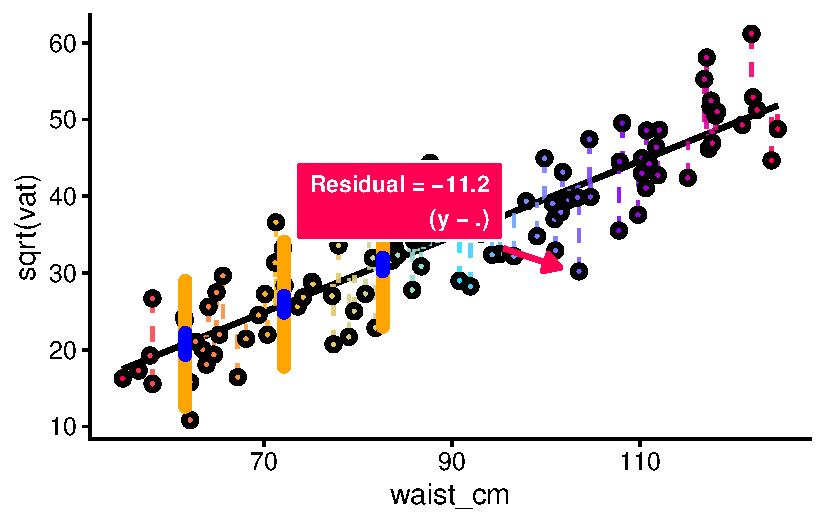
\includegraphics[keepaspectratio]{index_files/figure-pdf/unnamed-chunk-57-1.pdf}}

Few statistical ideas are as powerful and enduring as regression. From
nineteenth-century studies of human height to modern analyses of
inequality, elections, or climate change, regression has become the
universal language for describing how one variable changes when another
changes. It is at once a mathematical technique, a conceptual framework
for explanation, and a bridge between data and theory. 1. What
Regression Is At its core, regression is about relationships. It helps
us answer questions such as: How does income change with education? How
does voter turnout vary with local unemployment? How does CO₂
concentration affect temperature over time? Regression provides a way to
quantify these relationships by fitting a mathematical
function---usually a straight line---that best summarizes how a response
variable changes accordingly.

Regression extends beyond correlation. A correlation coefficient only
tells us that two variables move together and how strongly, but not how
much change in one variable corresponds to change in the other.
Regression quantifies that link. For example, suppose education and
earnings are positively correlated. Regression lets us estimate how much
additional income is associated with each additional year of schooling.
The slope of the regression line becomes a concrete measure of marginal
effect. Moreover, regression introduces directionality---we decide which
variable is the explanatory (on the x-axis) and which is the response
(on the y-axis). That decision reflects a theoretical claim about causal
order, even if regression itself does not prove causation.

*The Principle of Least Squares

The power of regression lies in its method of fitting a line to data.
The ``best-fitting'' line is not arbitrary; it is determined by a
precise rule called the least squares criterion. Imagine a scatterplot
of data points. Each point lies some distance above or below the line.
These vertical distances---called residuals---represent prediction
errors. Regression chooses the line that minimizes the sum of the
squared residuals.

Why Regression Is Useful?

Regression is useful in at least three profound ways.

\begin{enumerate}
\def\labelenumi{(\alph{enumi})}
\tightlist
\item
  Prediction Regression provides a tool for prediction. Once we estimate
  a relationship, we can forecast the likely value of y for any new
  value of x.
\end{enumerate}

In social science, this means we can estimate, for instance, how voter
turnout might change if unemployment rises by one percentage point, or
how income inequality might shift with a change in taxation.

\begin{enumerate}
\def\labelenumi{(\alph{enumi})}
\setcounter{enumi}{1}
\tightlist
\item
  Explanation
\end{enumerate}

Regression helps identify which variables are associated with an outcome
and by how much. In this way, it serves as a bridge between theory and
data. A theoretical claim---say, that educational attainment increases
earnings---translates into an empirical statement about the size and
sign of a regression coefficient.

\begin{enumerate}
\def\labelenumi{(\alph{enumi})}
\setcounter{enumi}{2}
\tightlist
\item
  Control and Comparison
\end{enumerate}

In multiple regression, we can include several explanatory variables
simultaneously, allowing us to examine the independent association of
each while holding others constant. This capacity to ``control for''
confounding factors is what makes regression the backbone of modern
social science. It approximates the logic of experimentation in
observational data. 5. The Meaning of the Coefficients Each coefficient
in a regression equation represents a slope---a marginal relationship
between one explanatory variable and the outcome. The intercept gives a
baseline; the slope tells the direction and magnitude of change. Yet
interpretation always depends on units: a one-unit increase in x.x must
correspond to a meaningful, measurable change (for example, one year of
education, \$1,000 of income, or one percentage point of unemployment).
Regression's power comes from translating those abstract numbers into
substantive claims about the world.

\begin{Shaded}
\begin{Highlighting}[]
\FunctionTok{suppressPackageStartupMessages}\NormalTok{(\{}
  \FunctionTok{library}\NormalTok{(ggplot2); }\FunctionTok{library}\NormalTok{(dplyr); }\FunctionTok{library}\NormalTok{(purrr); }\FunctionTok{library}\NormalTok{(grid)}
\NormalTok{\})}

\CommentTok{\# {-}{-}{-}{-} Parameters {-}{-}{-}{-}}
\NormalTok{b0 }\OtherTok{\textless{}{-}} \FloatTok{1.1}\NormalTok{; b1 }\OtherTok{\textless{}{-}} \FloatTok{0.62}
\NormalTok{sig }\OtherTok{\textless{}{-}} \FloatTok{0.55}
\NormalTok{xpos }\OtherTok{\textless{}{-}} \FunctionTok{c}\NormalTok{(}\FloatTok{1.1}\NormalTok{, }\FloatTok{2.6}\NormalTok{, }\FloatTok{4.1}\NormalTok{)}
\NormalTok{halfw }\OtherTok{\textless{}{-}} \FloatTok{0.22}

\NormalTok{make\_half\_normal }\OtherTok{\textless{}{-}} \ControlFlowTok{function}\NormalTok{(x0, mu, sig, halfw, }\AttributeTok{n =} \DecValTok{280}\NormalTok{) \{}
\NormalTok{  y }\OtherTok{\textless{}{-}} \FunctionTok{seq}\NormalTok{(mu }\SpecialCharTok{{-}} \FloatTok{3.2}\SpecialCharTok{*}\NormalTok{sig, mu }\SpecialCharTok{+} \FloatTok{3.2}\SpecialCharTok{*}\NormalTok{sig, }\AttributeTok{length.out =}\NormalTok{ n)}
\NormalTok{  d }\OtherTok{\textless{}{-}} \FunctionTok{dnorm}\NormalTok{(y, mu, sig)}
\NormalTok{  s }\OtherTok{\textless{}{-}}\NormalTok{ halfw }\SpecialCharTok{/} \FunctionTok{max}\NormalTok{(d)}
  \FunctionTok{tibble}\NormalTok{(}\AttributeTok{x =}\NormalTok{ x0 }\SpecialCharTok{+}\NormalTok{ s}\SpecialCharTok{*}\NormalTok{d, }\AttributeTok{y =}\NormalTok{ y)}
\NormalTok{\}}

\NormalTok{xr }\OtherTok{\textless{}{-}} \FunctionTok{c}\NormalTok{(}\FunctionTok{min}\NormalTok{(xpos) }\SpecialCharTok{{-}} \FloatTok{1.2}\NormalTok{, }\FunctionTok{max}\NormalTok{(xpos) }\SpecialCharTok{+} \FloatTok{0.9}\NormalTok{)}
\NormalTok{regdf }\OtherTok{\textless{}{-}} \FunctionTok{tibble}\NormalTok{(}\AttributeTok{x =} \FunctionTok{seq}\NormalTok{(xr[}\DecValTok{1}\NormalTok{], xr[}\DecValTok{2}\NormalTok{], }\AttributeTok{length.out =} \DecValTok{400}\NormalTok{),}
                \AttributeTok{y =}\NormalTok{ b0 }\SpecialCharTok{+}\NormalTok{ b1}\SpecialCharTok{*}\NormalTok{x)}

\NormalTok{slices }\OtherTok{\textless{}{-}} \FunctionTok{imap\_dfr}\NormalTok{(xpos, \textbackslash{}(x0, i) \{}
\NormalTok{  mu }\OtherTok{\textless{}{-}}\NormalTok{ b0 }\SpecialCharTok{+}\NormalTok{ b1}\SpecialCharTok{*}\NormalTok{x0}
  \FunctionTok{make\_half\_normal}\NormalTok{(x0, mu, sig, halfw) }\SpecialCharTok{|\textgreater{}}
    \FunctionTok{mutate}\NormalTok{(}\AttributeTok{slice =} \FunctionTok{factor}\NormalTok{(i))}
\NormalTok{\})}

\NormalTok{vlines }\OtherTok{\textless{}{-}} \FunctionTok{tibble}\NormalTok{(}\AttributeTok{x0 =}\NormalTok{ xpos,}
                 \AttributeTok{y0 =} \FunctionTok{min}\NormalTok{(regdf}\SpecialCharTok{$}\NormalTok{y) }\SpecialCharTok{{-}} \FloatTok{3.0}\SpecialCharTok{*}\NormalTok{sig,}
                 \AttributeTok{y1 =} \FunctionTok{max}\NormalTok{(regdf}\SpecialCharTok{$}\NormalTok{y) }\SpecialCharTok{+} \FloatTok{2.2}\SpecialCharTok{*}\NormalTok{sig)}

\NormalTok{labsdf }\OtherTok{\textless{}{-}} \FunctionTok{tibble}\NormalTok{(}
  \AttributeTok{x =}\NormalTok{ xpos }\SpecialCharTok{+}\NormalTok{ halfw }\SpecialCharTok{+} \FloatTok{0.12}\NormalTok{,}
  \AttributeTok{y =}\NormalTok{ b0 }\SpecialCharTok{+}\NormalTok{ b1}\SpecialCharTok{*}\NormalTok{xpos,}
  \AttributeTok{lab =} \FunctionTok{c}\NormalTok{(}\StringTok{"N(beta[1]*x[1] + beta[0], sigma\^{}2)"}\NormalTok{,}
          \StringTok{"N(beta[1]*x[2] + beta[0], sigma\^{}2)"}\NormalTok{,}
          \StringTok{"N(beta[1]*x[3] + beta[0], sigma\^{}2)"}\NormalTok{)}
\NormalTok{)}

\NormalTok{xlim }\OtherTok{\textless{}{-}} \FunctionTok{c}\NormalTok{(xr[}\DecValTok{1}\NormalTok{] }\SpecialCharTok{{-}} \FloatTok{0.1}\NormalTok{, xr[}\DecValTok{2}\NormalTok{] }\SpecialCharTok{+} \FloatTok{0.3}\NormalTok{)}
\NormalTok{ylim }\OtherTok{\textless{}{-}} \FunctionTok{range}\NormalTok{(vlines}\SpecialCharTok{$}\NormalTok{y0, vlines}\SpecialCharTok{$}\NormalTok{y1)}

\FunctionTok{ggplot}\NormalTok{() }\SpecialCharTok{+}
  \FunctionTok{theme\_void}\NormalTok{(}\AttributeTok{base\_size =} \DecValTok{14}\NormalTok{) }\SpecialCharTok{+}

  \CommentTok{\# Axes with arrowheads}
  \FunctionTok{annotate}\NormalTok{(}\StringTok{"segment"}\NormalTok{,}
           \AttributeTok{x =}\NormalTok{ xlim[}\DecValTok{1}\NormalTok{], }\AttributeTok{xend =}\NormalTok{ xlim[}\DecValTok{2}\NormalTok{], }\AttributeTok{y =}\NormalTok{ ylim[}\DecValTok{1}\NormalTok{], }\AttributeTok{yend =}\NormalTok{ ylim[}\DecValTok{1}\NormalTok{],}
           \AttributeTok{linewidth =}\NormalTok{ .}\DecValTok{8}\NormalTok{, }\AttributeTok{arrow =} \FunctionTok{arrow}\NormalTok{(}\AttributeTok{type =} \StringTok{"closed"}\NormalTok{, }\AttributeTok{length =} \FunctionTok{unit}\NormalTok{(}\FloatTok{0.22}\NormalTok{,}\StringTok{"cm"}\NormalTok{))) }\SpecialCharTok{+}
  \FunctionTok{annotate}\NormalTok{(}\StringTok{"segment"}\NormalTok{,}
           \AttributeTok{x =}\NormalTok{ xlim[}\DecValTok{1}\NormalTok{], }\AttributeTok{xend =}\NormalTok{ xlim[}\DecValTok{1}\NormalTok{], }\AttributeTok{y =}\NormalTok{ ylim[}\DecValTok{1}\NormalTok{], }\AttributeTok{yend =}\NormalTok{ ylim[}\DecValTok{2}\NormalTok{],}
           \AttributeTok{linewidth =}\NormalTok{ .}\DecValTok{8}\NormalTok{, }\AttributeTok{arrow =} \FunctionTok{arrow}\NormalTok{(}\AttributeTok{type =} \StringTok{"closed"}\NormalTok{, }\AttributeTok{length =} \FunctionTok{unit}\NormalTok{(}\FloatTok{0.22}\NormalTok{,}\StringTok{"cm"}\NormalTok{))) }\SpecialCharTok{+}

  \CommentTok{\# Ticks/labels and axis titles}
  \FunctionTok{annotate}\NormalTok{(}\StringTok{"segment"}\NormalTok{, }\AttributeTok{x =}\NormalTok{ xpos, }\AttributeTok{xend =}\NormalTok{ xpos, }\AttributeTok{y =}\NormalTok{ ylim[}\DecValTok{1}\NormalTok{], }\AttributeTok{yend =}\NormalTok{ ylim[}\DecValTok{1}\NormalTok{] }\SpecialCharTok{+} \FloatTok{0.09}\NormalTok{, }\AttributeTok{linewidth=}\NormalTok{.}\DecValTok{6}\NormalTok{) }\SpecialCharTok{+}
  \FunctionTok{annotate}\NormalTok{(}\StringTok{"text"}\NormalTok{, }\AttributeTok{x =}\NormalTok{ xpos, }\AttributeTok{y =}\NormalTok{ ylim[}\DecValTok{1}\NormalTok{] }\SpecialCharTok{+} \FloatTok{0.23}\NormalTok{,}
           \AttributeTok{label =} \FunctionTok{c}\NormalTok{(}\StringTok{"x[1]"}\NormalTok{,}\StringTok{"x[2]"}\NormalTok{,}\StringTok{"x[3]"}\NormalTok{), }\AttributeTok{parse =} \ConstantTok{TRUE}\NormalTok{, }\AttributeTok{size =} \FloatTok{4.6}\NormalTok{) }\SpecialCharTok{+}
  \FunctionTok{annotate}\NormalTok{(}\StringTok{"text"}\NormalTok{, }\AttributeTok{x =} \FunctionTok{mean}\NormalTok{(xlim), }\AttributeTok{y =}\NormalTok{ ylim[}\DecValTok{1}\NormalTok{] }\SpecialCharTok{{-}} \FloatTok{0.05}\NormalTok{, }\AttributeTok{label =} \StringTok{"x"}\NormalTok{, }\AttributeTok{vjust =} \DecValTok{1}\NormalTok{, }\AttributeTok{size =} \DecValTok{5}\NormalTok{) }\SpecialCharTok{+}
  \FunctionTok{annotate}\NormalTok{(}\StringTok{"text"}\NormalTok{, }\AttributeTok{x =}\NormalTok{ xlim[}\DecValTok{1}\NormalTok{] }\SpecialCharTok{{-}} \FloatTok{0.08}\NormalTok{, }\AttributeTok{y =} \FunctionTok{mean}\NormalTok{(ylim), }\AttributeTok{label =} \StringTok{"y"}\NormalTok{, }\AttributeTok{angle =} \DecValTok{90}\NormalTok{, }\AttributeTok{size =} \DecValTok{5}\NormalTok{) }\SpecialCharTok{+}

  \CommentTok{\# Regression line (black)}
  \FunctionTok{geom\_line}\NormalTok{(}\AttributeTok{data =}\NormalTok{ regdf, }\FunctionTok{aes}\NormalTok{(x, y), }\AttributeTok{linewidth =} \FloatTok{0.8}\NormalTok{, }\AttributeTok{lineend =} \StringTok{"round"}\NormalTok{) }\SpecialCharTok{+}

  \CommentTok{\# Vertical guides (black)}
  \FunctionTok{geom\_segment}\NormalTok{(}\AttributeTok{data =}\NormalTok{ vlines, }\FunctionTok{aes}\NormalTok{(}\AttributeTok{x =}\NormalTok{ x0, }\AttributeTok{xend =}\NormalTok{ x0, }\AttributeTok{y =}\NormalTok{ y0, }\AttributeTok{yend =}\NormalTok{ y1), }\AttributeTok{linewidth =} \FloatTok{0.7}\NormalTok{) }\SpecialCharTok{+}

  \CommentTok{\# Half{-}normals (RIGHT side) — now RED}
  \FunctionTok{geom\_path}\NormalTok{(}\AttributeTok{data =}\NormalTok{ slices, }\FunctionTok{aes}\NormalTok{(x, y, }\AttributeTok{group =}\NormalTok{ slice), }\AttributeTok{linewidth =} \FloatTok{0.9}\NormalTok{, }\AttributeTok{color =} \StringTok{"red"}\NormalTok{) }\SpecialCharTok{+}

  \CommentTok{\# Mean tick on each slice (black)}
  \FunctionTok{geom\_segment}\NormalTok{(}\AttributeTok{data =} \FunctionTok{tibble}\NormalTok{(}\AttributeTok{x0 =}\NormalTok{ xpos, }\AttributeTok{y0 =}\NormalTok{ b0 }\SpecialCharTok{+}\NormalTok{ b1}\SpecialCharTok{*}\NormalTok{xpos),}
               \FunctionTok{aes}\NormalTok{(}\AttributeTok{x =}\NormalTok{ x0 }\SpecialCharTok{{-}} \FloatTok{0.02}\NormalTok{, }\AttributeTok{xend =}\NormalTok{ x0 }\SpecialCharTok{+} \FloatTok{0.18}\NormalTok{, }\AttributeTok{y =}\NormalTok{ y0, }\AttributeTok{yend =}\NormalTok{ y0),}
               \AttributeTok{linewidth =} \FloatTok{0.8}\NormalTok{) }\SpecialCharTok{+}

  \CommentTok{\# N(·) labels}
  \FunctionTok{geom\_text}\NormalTok{(}\AttributeTok{data =}\NormalTok{ labsdf,}
            \FunctionTok{aes}\NormalTok{(}\AttributeTok{x =}\NormalTok{ x, }\AttributeTok{y =}\NormalTok{ y, }\AttributeTok{label =}\NormalTok{ lab),}
            \AttributeTok{parse =} \ConstantTok{TRUE}\NormalTok{, }\AttributeTok{hjust =} \DecValTok{0}\NormalTok{, }\AttributeTok{vjust =} \FloatTok{0.5}\NormalTok{, }\AttributeTok{size =} \FloatTok{4.8}\NormalTok{) }\SpecialCharTok{+}

  \CommentTok{\# E(Y)=... label + arrow}
  \FunctionTok{annotate}\NormalTok{(}\StringTok{"text"}\NormalTok{,}
           \AttributeTok{x =}\NormalTok{ xpos[}\DecValTok{2}\NormalTok{] }\SpecialCharTok{{-}} \FloatTok{0.10}\NormalTok{, }\AttributeTok{y =}\NormalTok{ b0 }\SpecialCharTok{+}\NormalTok{ b1}\SpecialCharTok{*}\NormalTok{xpos[}\DecValTok{2}\NormalTok{] }\SpecialCharTok{+} \FloatTok{0.95}\NormalTok{,}
           \AttributeTok{label =} \StringTok{"E(Y) == beta[1]*x + beta[0]"}\NormalTok{, }\AttributeTok{parse =} \ConstantTok{TRUE}\NormalTok{, }\AttributeTok{size =} \FloatTok{5.2}\NormalTok{) }\SpecialCharTok{+}
  \FunctionTok{annotate}\NormalTok{(}\StringTok{"segment"}\NormalTok{,}
           \AttributeTok{x =}\NormalTok{ xpos[}\DecValTok{2}\NormalTok{] }\SpecialCharTok{+} \FloatTok{0.02}\NormalTok{, }\AttributeTok{y =}\NormalTok{ b0 }\SpecialCharTok{+}\NormalTok{ b1}\SpecialCharTok{*}\NormalTok{xpos[}\DecValTok{2}\NormalTok{] }\SpecialCharTok{+} \FloatTok{0.80}\NormalTok{,}
           \AttributeTok{xend =}\NormalTok{ xpos[}\DecValTok{2}\NormalTok{] }\SpecialCharTok{+} \FloatTok{0.22}\NormalTok{, }\AttributeTok{yend =}\NormalTok{ b0 }\SpecialCharTok{+}\NormalTok{ b1}\SpecialCharTok{*}\NormalTok{xpos[}\DecValTok{2}\NormalTok{] }\SpecialCharTok{+} \FloatTok{0.32}\NormalTok{,}
           \AttributeTok{arrow =} \FunctionTok{arrow}\NormalTok{(}\AttributeTok{type =} \StringTok{"closed"}\NormalTok{, }\AttributeTok{length =} \FunctionTok{unit}\NormalTok{(}\FloatTok{0.22}\NormalTok{,}\StringTok{"cm"}\NormalTok{)),}
           \AttributeTok{linewidth =} \FloatTok{0.6}\NormalTok{) }\SpecialCharTok{+}

  \CommentTok{\# Reference note below the x{-}axis}
  \FunctionTok{annotate}\NormalTok{(}\StringTok{"text"}\NormalTok{,}
           \AttributeTok{x =} \FunctionTok{mean}\NormalTok{(xlim), }\AttributeTok{y =}\NormalTok{ ylim[}\DecValTok{1}\NormalTok{] }\SpecialCharTok{{-}} \FloatTok{0.56}\NormalTok{,}
           \AttributeTok{label =} \StringTok{"Reference: Simple Linear Regression Model  —  Introductory Statistics (Shafer and Zhang), UC Davis Stat"}\NormalTok{,}
           \AttributeTok{size =} \DecValTok{4}\NormalTok{, }\AttributeTok{hjust =} \FloatTok{0.5}\NormalTok{) }\SpecialCharTok{+}

  \FunctionTok{coord\_cartesian}\NormalTok{(}\AttributeTok{xlim =}\NormalTok{ xlim, }\AttributeTok{ylim =}\NormalTok{ ylim, }\AttributeTok{clip =} \StringTok{"off"}\NormalTok{) }\SpecialCharTok{+}
  \FunctionTok{theme}\NormalTok{(}\AttributeTok{plot.margin =} \FunctionTok{margin}\NormalTok{(}\DecValTok{26}\NormalTok{, }\DecValTok{40}\NormalTok{, }\DecValTok{40}\NormalTok{, }\DecValTok{32}\NormalTok{))}
\end{Highlighting}
\end{Shaded}

\pandocbounded{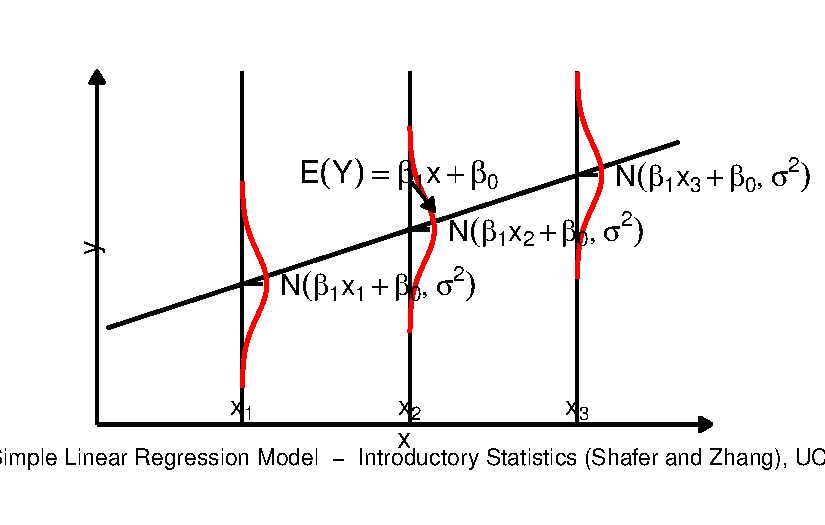
\includegraphics[keepaspectratio]{index_files/figure-pdf/unnamed-chunk-58-1.pdf}}

\section{Summary}\label{summary-2}

\begin{itemize}
\tightlist
\item
  A \textbf{regression line} predicts how \(y\) changes as \(x\)
  changes.\\
\item
  The \textbf{intercept} (\(a\)) is the predicted value of \(y\) when
  \(x = 0\).\\
\item
  The \textbf{slope} (\(b\)) indicates the predicted change in \(y\) for
  a one-unit change in \(x\).\\
\item
  \textbf{Residuals} are the differences between observed and predicted
  values of \(y\).\\
\item
  \textbf{Ordinary Least Squares (OLS)} estimates \(a\) and \(b\) by
  minimizing the \textbf{sum of squared residuals}.\\
\item
  \textbf{\(R^2\)} indicates the proportion of variation in \(y\)
  explained by \(x\).\\
\item
  Regression relationships are \emph{associative}, not causal.
\end{itemize}

\bookmarksetup{startatroot}

\chapter{Chapter 13: Multivariate
Regression}\label{chapter-13-multivariate-regression}

The preceding chapter examined how regression analysis models the
connection between two variables: a dependent variable \(y\) and an
independent variable \(x\). Through \textbf{bivariate regression}, we
developed methods to quantify how changes in \(x\) correspond to changes
in \(y\), and we measured the degree of association between these
variables using the \(R^2\) statistic.

The social scientific outcomes rarely result from a single cause
operating in isolation. As a result, we need to have an estimation
machinery that allows us to include more than one independent variable.
Consider earnings: educational attainment matters, but so do years of
professional experience, regional labor markets, sectoral employment,
and numerous additional considerations. Similarly, electoral
participation reflects a confluence of factors including economic
conditions, party system characteristics, resource mobilization efforts,
population attributes, and the structural features of political
institutions. Analyzing these multifaceted relationships requires
\textbf{multivariate regression}---alternatively termed \textbf{multiple
regression}---a framework that permits simultaneous examination of how a
dependent variable relates to \emph{multiple} independent variables.

This chapter introduces the theory and practice of multivariate
regression. We will learn how to estimate, interpret, and test models
with multiple predictors. We will also encounter \textbf{matrix
notation}, a compact mathematical language that makes multivariate
regression both elegant and computationally tractable.

\section{Why Introduce Multiple Independent
Variables?}\label{why-introduce-multiple-independent-variables}

Why should we include more than one predictor in a regression model?
There are at least three compelling reasons:

\subsection{1. Explanation: More is
Better}\label{explanation-more-is-better}

From an explanatory perspective, social phenomena rarely have a single
cause. If we want to \emph{understand} variation in an outcome, we
should account for the multiple factors that shape it. A richer
model---one that includes several relevant predictors---provides a more
complete and realistic explanation.

To illustrate, imagine we are investigating \textbf{the generosity of
welfare states}, operationalized through a decommodification scale
(which quantifies the extent to which social programs diminish citizens'
reliance on market participation for social reproduction). A
specification that includes gross domestic production alone may account
for a portion of cross-national variation in welfare provision. However,
a theoretically richer specification would incorporate additional
predictors: the organizational capacity of trade unions, the electoral
strength of left-wing political parties, the demographic composition of
the society, and path-dependent institutional inheritances from earlier
periods of state formation. Each predictor represents a conceptually
distinct mechanism through which welfare generosity may emerge.

\subsection{2. Control: Holding Things
Constant}\label{control-holding-things-constant}

One of the primary advantages of multiple regression is its capacity to
\textbf{account for potentially confounding factors}. By incorporating
several explanatory variables simultaneously, we can isolate the
relationship between a focal predictor and the response variable
\emph{while keeping other predictors fixed}. Researchers often refer to
this process as ``partialling out'' or ``netting out'' the influence of
additional variables.

Consider the following empirical puzzle: wealthier nations typically
exhibit more generous welfare systems. Does national affluence directly
\emph{produce} expansive social policies? Alternatively, perhaps
economic prosperity coincides with robust organized labor, and it is
union strength---rather than wealth per se---that drives welfare state
development.

Multiple regression provides analytical leverage on this question. When
we simultaneously include both GDP and unionization rates as predictors,
we can estimate each variable's \emph{distinct} association with the
outcome. The GDP coefficient now captures how welfare generosity varies
with national income, \textbf{with unionization held fixed}. This
statistical strategy mimics experimental control within observational
research designs.

\subsection{3. Specification: Removing Omitted
Variables}\label{specification-removing-omitted-variables}

A regression model is \textbf{correctly specified} when it includes all
relevant predictors and excludes irrelevant ones. If we omit an
important variable---one that is correlated both with the outcome and
with an included predictor---our estimates will be \textbf{biased}. This
problem is known as \textbf{omitted variable bias}.

Multivariate regression helps us address this problem by moving
variables out of the error term \(e\) and into the model itself. By
explicitly including relevant predictors, we reduce the risk that
unobserved factors are distorting our estimates.

In short, multivariate regression is essential for explanation, control,
and correct specification. It is the workhorse of empirical social
science.

\begin{center}\rule{0.5\linewidth}{0.5pt}\end{center}

\section{The Multivariate Regression
Equation}\label{the-multivariate-regression-equation}

The general form of a multivariate regression model with \(k\)
predictors is:

\[
y = \beta_0 + \beta_1 x_1 + \beta_2 x_2 + \ldots + \beta_k x_k + e
\]

where:

\begin{itemize}
\item
  \(y\) is the \textbf{response/outcome variable} (also called the
  dependent variable)
\item
  \(x_1, x_2, \ldots, x_k\) are the \textbf{explanatory variables} (also
  called independent variables or predictors)
\item
  \(\beta_0\) is the \textbf{intercept}, representing the predicted
  value of \(y\) when all \(x\) variables equal zero
\item
  \(\beta_1, \beta_2, \ldots, \beta_k\) are the \textbf{slope
  coefficients}, each representing the expected change in \(y\) for a
  one-unit increase in the corresponding \(x\), \emph{holding all other
  variables constant}
\item
  \(e\) is the \textbf{error term}, representing unexplained variation
  in \(y\)
\end{itemize}

\subsection{Example: Economic Development and Welfare State
Generosity}\label{example-economic-development-and-welfare-state-generosity}

Suppose we believe that welfare state generosity (measured by a
decommodification index) depends on two factors: \textbf{economic
development} (measured by GDP per capita) and \textbf{the political
strength of social democratic parties} (measured by the percentage of
legislative seats held by left parties).

We can write this as:

\[
y = \beta_0 + \beta_1 x_1 + \beta_2 x_2 + e
\]

where:

\begin{itemize}
\tightlist
\item
  \(y\) = decommodification index
\item
  \(x_1\) = GDP per capita (in thousands of dollars)
\item
  \(x_2\) = percentage of legislative/cabinet seats held by social
  democratic or labour parties
\item
  \(e\) = error term
\end{itemize}

This model allows us to estimate the \emph{independent} effect of
economic development, controlling for left party strength, and the
\emph{independent} effect of left party strength, controlling for
economic development.

\begin{center}\rule{0.5\linewidth}{0.5pt}\end{center}

\section{Interpreting Multivariate Regression
Coefficients}\label{interpreting-multivariate-regression-coefficients}

The key difference between bivariate and multivariate regression is that
in multivariate regression, each coefficient represents a
\textbf{partial effect}---the association between one predictor and the
outcome, \emph{holding all other predictors constant}.

Consider the model:

\[
y = \beta_0 + \beta_1 x_1 + \beta_2 x_2 + e
\]

The coefficient \(\beta_1\) tells us: \textbf{for a one-unit increase in
\(x_1\), \(y\) is expected to change by \(\beta_1\) units, holding
\(x_2\) constant}.

Similarly, \(\beta_2\) tells us: \textbf{for a one-unit increase in
\(x_2\), \(y\) is expected to change by \(\beta_2\) units, holding
\(x_1\) constant}.

This ``holding constant'' language is crucial. It distinguishes the
\emph{partial} association (adjusting for other variables) from the
\emph{marginal} association (ignoring other variables).

\subsection{Example Interpretation}\label{example-interpretation}

Suppose we estimate the following model for 18 OECD countries:

\[
\hat{y} = 11.18 + 1.17 x_1 + 1.15 x_2
\]

where:

\begin{itemize}
\tightlist
\item
  \(y\) = decommodification index
\item
  \(x_1\) = GDP per capita (in thousands of dollars)
\item
  \(x_2\) = percentage of seats held by left parties
\end{itemize}

\textbf{Interpretation and Discussion:}

\begin{itemize}
\item
  \textbf{Intercept (\(\hat{\beta}_0 = 11.18\)):} The baseline value of
  the decommodification index when GDP and left party representation
  both equal zero is 11.18. (Note that this value has limited practical
  interpretation since no observed countries fall at this baseline.)
\item
  \textbf{GDP coefficient (\(\hat{\beta}_1 = 1.17\)):} For each
  additional \$1,000 in GDP per capita, the decommodification index
  rises by 1.17 points, on average, \emph{when controlling for left
  party representation}.
\item
  \textbf{Left party coefficient (\(\hat{\beta}_2 = 1.15\)):} Each
  one-percentage-point gain in left party seats corresponds to a
  1.15-point higher decommodification index, on average, \emph{when
  controlling for GDP}.
\end{itemize}

\section{\texorpdfstring{Observe the precise terminology employed here:
``rises by,'' ``corresponds to,'' and ``when controlling for.'' This
language emphasizes that our regression coefficients represent
statistical \emph{relationships} rather than established \emph{causal
mechanisms}.}{Observe the precise terminology employed here: ``rises by,'' ``corresponds to,'' and ``when controlling for.'' This language emphasizes that our regression coefficients represent statistical relationships rather than established causal mechanisms.}}\label{observe-the-precise-terminology-employed-here-rises-by-corresponds-to-and-when-controlling-for.-this-language-emphasizes-that-our-regression-coefficients-represent-statistical-relationships-rather-than-established-causal-mechanisms.}

\section{Matrix Notation for Multivariate
Regression}\label{matrix-notation-for-multivariate-regression}

When working with multiple predictors, writing out each term separately
becomes cumbersome. \textbf{Matrix notation} provides a compact and
elegant way to express multivariate regression models. It also forms the
basis for computational algorithms that estimate regression
coefficients.

\subsection{Why Matrices?}\label{why-matrices}

Suppose we have \(n\) observations and \(k\) predictors. We can write
\(n\) separate regression equations:

\[
\begin{aligned}
y_1 &= \beta_0 + \beta_1 x_{11} + \beta_2 x_{21} + \ldots + \beta_k x_{k1} + e_1 \\
y_2 &= \beta_0 + \beta_1 x_{12} + \beta_2 x_{22} + \ldots + \beta_k x_{k2} + e_2 \\
&\vdots \\
y_n &= \beta_0 + \beta_1 x_{1n} + \beta_2 x_{2n} + \ldots + \beta_k x_{kn} + e_n
\end{aligned}
\]

This is tedious. Matrix notation allows us to write all \(n\) equations
as a single compact expression.

\subsection{Terminology}\label{terminology}

Before proceeding, let's discuss and review some basic matrix
terminology:

\begin{itemize}
\item
  A \textbf{scalar} is a single number (e.g., \(5\), \(-2.3\)).
\item
  A \textbf{vector} is a matrix with just one column (size
  \(n \times 1\)). Vectors are typically denoted with lowercase bold
  letters: \(\mathbf{y}\), \(\mathbf{x}\).
\item
  A \textbf{matrix} is a rectangular array of numbers with \(n\) rows
  and \(m\) columns (size \(n \times m\)). Matrices are typically
  denoted with uppercase bold letters: \(\mathbf{X}\), \(\mathbf{A}\).
\end{itemize}

\subsection{The Matrix Form of the Regression
Model}\label{the-matrix-form-of-the-regression-model}

We can express the multivariate regression model in matrix form as:

\[
\mathbf{y} = \mathbf{X} \boldsymbol{\beta} + \mathbf{e}
\]

where:

\begin{itemize}
\tightlist
\item
  \(\mathbf{y}\) is an \(n \times 1\) \textbf{vector of responses}:
\end{itemize}

\[
\mathbf{y} = \begin{pmatrix} y_1 \\ y_2 \\ \vdots \\ y_n \end{pmatrix}
\]

\begin{itemize}
\tightlist
\item
  \(\mathbf{X}\) is an \(n \times (k+1)\) \textbf{design matrix}
  containing the values of the predictors (plus a column of 1's for the
  intercept):
\end{itemize}

\[
\mathbf{X} = \begin{pmatrix}
1 & x_{11} & x_{21} & \cdots & x_{k1} \\
1 & x_{12} & x_{22} & \cdots & x_{k2} \\
\vdots & \vdots & \vdots & \ddots & \vdots \\
1 & x_{1n} & x_{2n} & \cdots & x_{kn}
\end{pmatrix}
\]

\begin{itemize}
\tightlist
\item
  \(\boldsymbol{\beta}\) is a \((k+1) \times 1\) \textbf{vector of
  coefficients}:
\end{itemize}

\[
\boldsymbol{\beta} = \begin{pmatrix} \beta_0 \\ \beta_1 \\ \beta_2 \\ \vdots \\ \beta_k \end{pmatrix}
\]

\begin{itemize}
\tightlist
\item
  \(\mathbf{e}\) is an \(n \times 1\) \textbf{vector of errors}:
\end{itemize}

\[
\mathbf{e} = \begin{pmatrix} e_1 \\ e_2 \\ \vdots \\ e_n \end{pmatrix}
\]

This single equation,
\(\mathbf{y} = \mathbf{X} \boldsymbol{\beta} + \mathbf{e}\), encodes all
\(n\) regression equations simultaneously.

\begin{center}\rule{0.5\linewidth}{0.5pt}\end{center}

\section{Estimating Regression Coefficients with
Matrices}\label{estimating-regression-coefficients-with-matrices}

In bivariate regression, we estimated the slope \(\hat{\beta}_1\) using
the formula:

\[
\hat{\beta}_1 = \frac{\sum (x_i - \bar{x})(y_i - \bar{y})}{\sum (x_i - \bar{x})^2}
\]

In multivariate regression, the formula generalizes to:

\[
\hat{\boldsymbol{\beta}} = (\mathbf{X}'\mathbf{X})^{-1} \mathbf{X}' \mathbf{y}
\]

where:

\begin{itemize}
\tightlist
\item
  \(\mathbf{X}'\) is the \textbf{transpose} of \(\mathbf{X}\) (rows
  become columns, columns become rows)
\item
  \((\mathbf{X}'\mathbf{X})^{-1}\) is the \textbf{inverse} of the matrix
  \(\mathbf{X}'\mathbf{X}\)
\end{itemize}

This formula is the \textbf{matrix solution to the least squares
problem}. It minimizes the sum of squared residuals, just as in
bivariate regression, but now accounts for multiple predictors
simultaneously.

\subsection{What Do These Matrix Operations
Mean?}\label{what-do-these-matrix-operations-mean}

\begin{itemize}
\item
  \textbf{\(\mathbf{X}'\mathbf{X}\)} is a \((k+1) \times (k+1)\) matrix
  that contains information about the \textbf{variances and covariances}
  among the predictors. It summarizes how the \(x\) variables relate to
  one another.
\item
  \textbf{\(\mathbf{X}'\mathbf{y}\)} is a \((k+1) \times 1\) vector that
  contains information about the \textbf{covariances between each
  predictor and the response}. When the data are ``demeaned'' (centered
  around their means), this is proportional to the covariance of \(y\)
  with each \(x\).
\item
  \textbf{\((\mathbf{X}'\mathbf{X})^{-1}\)} adjusts for the
  \textbf{intercorrelations among the predictors}. If the predictors are
  highly correlated with one another, this matrix reflects that
  dependence, which affects the precision of the coefficient estimates.
\end{itemize}

In short, the formula
\(\hat{\boldsymbol{\beta}} = (\mathbf{X}'\mathbf{X})^{-1} \mathbf{X}' \mathbf{y}\)
says:

\begin{quote}
The estimates of \(\boldsymbol{\beta}\) result from scaling the
information about the association between the \(x\)'s and \(y\) by the
information about the intercorrelation among the \(x\)'s.
\end{quote}

This is conceptually similar to the bivariate case, but now extended to
multiple dimensions.

\begin{center}\rule{0.5\linewidth}{0.5pt}\end{center}

\section{Residuals, Sum of Squared Residuals, and Error
Variance}\label{residuals-sum-of-squared-residuals-and-error-variance}

Just as in bivariate regression, we compute \textbf{residuals} as the
difference between observed and predicted values:

\[
\hat{\mathbf{e}} = \mathbf{y} - \mathbf{X} \hat{\boldsymbol{\beta}}
\]

The \textbf{sum of squared residuals (SSR)} is:

\[
\text{SSR} = \hat{\mathbf{e}}' \hat{\mathbf{e}} = \sum_{i=1}^n \hat{e}_i^2
\]

The \textbf{error variance} is the SSR divided by the degrees of
freedom:

\[
\hat{\sigma}^2 = \frac{\text{SSR}}{n - k - 1} = \frac{\hat{\mathbf{e}}' \hat{\mathbf{e}}}{n - k - 1}
\]

where \(n\) is the sample size and \(k\) is the number of predictors
(not including the intercept). The degrees of freedom are \(n - k - 1\)
because we estimate \(k + 1\) parameters
(\(\beta_0, \beta_1, \ldots, \beta_k\)).

\subsection{Variance and Standard Errors of
Coefficients}\label{variance-and-standard-errors-of-coefficients}

The \textbf{variance-covariance matrix} of \(\hat{\boldsymbol{\beta}}\)
is:

\[
\text{Var}(\hat{\boldsymbol{\beta}}) = \hat{\sigma}^2 (\mathbf{X}'\mathbf{X})^{-1}
\]

This is a \((k+1) \times (k+1)\) matrix. The diagonal elements give the
variances of each coefficient; the off-diagonal elements give the
covariances between pairs of coefficients.

The \textbf{standard error} of \(\hat{\beta}_j\) is:

\[
\text{SE}(\hat{\beta}_j) = \sqrt{\text{Var}(\hat{\beta}_j)}
\]

These standard errors are used to construct confidence intervals and
conduct hypothesis tests.

\begin{center}\rule{0.5\linewidth}{0.5pt}\end{center}

\section{Comparing Bivariate and Multivariate
Regression}\label{comparing-bivariate-and-multivariate-regression}

The table below summarizes the key formulas for bivariate and
multivariate regression:

\begin{longtable}[]{@{}
  >{\raggedright\arraybackslash}p{(\linewidth - 4\tabcolsep) * \real{0.1818}}
  >{\raggedright\arraybackslash}p{(\linewidth - 4\tabcolsep) * \real{0.3818}}
  >{\raggedright\arraybackslash}p{(\linewidth - 4\tabcolsep) * \real{0.4364}}@{}}
\toprule\noalign{}
\begin{minipage}[b]{\linewidth}\raggedright
Quantity
\end{minipage} & \begin{minipage}[b]{\linewidth}\raggedright
Bivariate Regression
\end{minipage} & \begin{minipage}[b]{\linewidth}\raggedright
Multivariate Regression
\end{minipage} \\
\midrule\noalign{}
\endhead
\bottomrule\noalign{}
\endlastfoot
\textbf{Slope} &
\(\hat{\beta}_1 = \frac{\sum (x_i - \bar{x})(y_i - \bar{y})}{\sum (x_i - \bar{x})^2}\)
&
\(\hat{\boldsymbol{\beta}} = (\mathbf{X}'\mathbf{X})^{-1} \mathbf{X}' \mathbf{y}\) \\
\textbf{Residuals} & \(\hat{e}_i = y_i - \hat{y}_i\) &
\(\hat{\mathbf{e}} = \mathbf{y} - \mathbf{X} \hat{\boldsymbol{\beta}}\) \\
\textbf{SSR} & \(\text{SSR} = \sum \hat{e}_i^2\) &
\(\text{SSR} = \hat{\mathbf{e}}' \hat{\mathbf{e}}\) \\
\textbf{Error Variance} &
\(\hat{\sigma}^2 = \frac{\sum \hat{e}_i^2}{n - 2}\) &
\(\hat{\sigma}^2 = \frac{\hat{\mathbf{e}}' \hat{\mathbf{e}}}{n - k - 1}\) \\
\textbf{Variance of \(\hat{\beta}\)} &
\(\text{Var}(\hat{\beta}_1) = \frac{\hat{\sigma}^2}{\sum (x_i - \bar{x})^2}\)
&
\(\text{Var}(\hat{\boldsymbol{\beta}}) = \hat{\sigma}^2 (\mathbf{X}'\mathbf{X})^{-1}\) \\
\textbf{Standard Error} &
\(\text{SE}(\hat{\beta}_1) = \sqrt{\text{Var}(\hat{\beta}_1)}\) &
\(\text{SE}(\hat{\beta}_j) = \sqrt{\text{Var}(\hat{\beta}_j)}\) \\
\end{longtable}

The multivariate formulas reduce to the bivariate formulas when
\(k = 1\) (one predictor).

\begin{center}\rule{0.5\linewidth}{0.5pt}\end{center}

\section{Hypothesis Testing and Statistical
Inference}\label{hypothesis-testing-and-statistical-inference}

\subsection{Testing Individual
Coefficients}\label{testing-individual-coefficients}

In multivariate regression, we often test the null hypothesis:

\[
H_0: \beta_j = 0
\]

This hypothesis asks: ``Is there a statistically significant association
between \(x_j\) and \(y\), controlling for all other predictors?''

The \textbf{\(t\)-statistic} for testing this hypothesis is:

\[
t = \frac{\hat{\beta}_j - 0}{\text{SE}(\hat{\beta}_j)} = \frac{\hat{\beta}_j}{\text{SE}(\hat{\beta}_j)}
\]

This statistic follows a \(t\)-distribution with \(n - k - 1\) degrees
of freedom.

A large \(t\)-statistic (in absolute value) and a small \(p\)-value
indicate that we can reject the null hypothesis. We conclude that
\(\beta_j\) is statistically significantly different from zero.

\subsection{Example: Testing Coefficients in the Welfare State
Model}\label{example-testing-coefficients-in-the-welfare-state-model}

Suppose we estimate the following model:

\[
\hat{y} = 11.18 + 1.17 x_1 + 1.15 x_2
\]

and obtain the following standard errors and \(t\)-statistics:

\begin{longtable}[]{@{}lllll@{}}
\toprule\noalign{}
Variable & Coefficient & Standard Error & \(t\)-statistic &
\(p\)-value \\
\midrule\noalign{}
\endhead
\bottomrule\noalign{}
\endlastfoot
Intercept & 11.18 & 6.04 & 1.85 & 0.08 \\
GDP (\(x_1\)) & 1.17 & 0.57 & 2.04 & 0.06 \\
Left party (\(x_2\)) & 1.15 & 0.61 & 1.87 & 0.08 \\
\end{longtable}

\textbf{Interpretation:}

\begin{itemize}
\item
  The \(t\)-statistic for GDP is \(t = 1.17 / 0.57 = 2.04\), with a
  \(p\)-value of 0.06. At the conventional \(\alpha = 0.05\) level, this
  is \emph{marginally} not significant. However, at \(\alpha = 0.10\),
  we would reject the null hypothesis and conclude that GDP is
  significantly associated with welfare state generosity, controlling
  for left party strength.
\item
  Similarly, the \(t\)-statistic for left party strength is
  \(t = 1.15 / 0.61 = 1.87\), with a \(p\)-value of 0.08. This is also
  marginally significant at \(\alpha = 0.10\).
\end{itemize}

These results suggest that both economic development and left party
strength are independently associated with welfare state generosity,
though the evidence is somewhat weak given the small sample size
(\(n = 18\)).

\begin{center}\rule{0.5\linewidth}{0.5pt}\end{center}

\section{\texorpdfstring{Goodness-of-Fit: \(R^2\) and the
\(F\)-Statistic}{Goodness-of-Fit: R\^{}2 and the F-Statistic}}\label{goodness-of-fit-r2-and-the-f-statistic}

\subsection{\texorpdfstring{\(R^2\): Proportion of Variance
Explained}{R\^{}2: Proportion of Variance Explained}}\label{r2-proportion-of-variance-explained}

Just as in bivariate regression, we can compute \(R^2\) to measure how
well the model fits the data:

\[
R^2 = \frac{\text{RegSS}}{\text{SST}} = 1 - \frac{\text{SSR}}{\text{SST}}
\]

where:

\begin{itemize}
\tightlist
\item
  \textbf{SST} (total sum of squares) = \(\sum (y_i - \bar{y})^2\)
\item
  \textbf{RegSS} (regression sum of squares) =
  \(\sum (\hat{y}_i - \bar{y})^2\)
\item
  \textbf{SSR} (sum of squared residuals) = \(\sum (y_i - \hat{y}_i)^2\)
\end{itemize}

\(R^2\) represents the \textbf{proportion of variation in \(y\)
explained by the model}. It ranges from 0 (no explanatory power) to 1
(perfect fit).

\textbf{Important:} In multivariate regression, \(R^2\) will
\emph{always} increase as we add more predictors, even if those
predictors have no real association with \(y\). For this reason,
\textbf{adjusted \(R^2\)} is sometimes used to penalize model
complexity:

\[
R^2_{\text{adj}} = 1 - \frac{\text{SSR} / (n - k - 1)}{\text{SST} / (n - 1)}
\]

\subsection{\texorpdfstring{The \(F\)-Statistic: Testing Overall Model
Significance}{The F-Statistic: Testing Overall Model Significance}}\label{the-f-statistic-testing-overall-model-significance}

The \textbf{\(F\)-statistic} tests the null hypothesis that \emph{all}
slope coefficients are zero:

\[
H_0: \beta_1 = \beta_2 = \ldots = \beta_k = 0
\]

The \(F\)-statistic is computed as:

\[
F = \frac{\text{RegSS} / k}{\text{SSR} / (n - k - 1)}
\]

This statistic follows an \(F\)-distribution with \(k\) numerator
degrees of freedom and \(n - k - 1\) denominator degrees of freedom.

A large \(F\)-statistic and a small \(p\)-value indicate that the model
as a whole is statistically significant---that is, at least one of the
predictors is significantly associated with the outcome.

\subsection{Example: Welfare State
Model}\label{example-welfare-state-model}

In our welfare state model, suppose:

\begin{itemize}
\tightlist
\item
  \(R^2 = 0.45\)
\item
  \(F = 6.07\) on 2 and 15 degrees of freedom, \(p = 0.01\)
\end{itemize}

\textbf{Interpretation:}

\begin{itemize}
\item
  The model explains \textbf{45\% of the variation} in welfare state
  generosity across the 18 countries.
\item
  The \(F\)-statistic is significant at \(p = 0.01\), indicating that
  the model as a whole is statistically significant. At least one of the
  predictors (GDP or left party strength) is significantly associated
  with the outcome.
\end{itemize}

\begin{center}\rule{0.5\linewidth}{0.5pt}\end{center}

\section{Model Assumptions}\label{model-assumptions}

Multivariate regression relies on the same assumptions as bivariate
regression. Violations of these assumptions can lead to biased
estimates, incorrect standard errors, or invalid hypothesis tests.

\subsection{1. Correct Specification}\label{correct-specification}

The model must be correctly specified, meaning:

\begin{itemize}
\tightlist
\item
  \textbf{Causality runs in one direction:} from the independent
  variables to the dependent variable (no reverse causation).
\item
  \textbf{The functional form is linear:} the relationship between \(y\)
  and each \(x\) is linear (or has been transformed to be linear).
\item
  \textbf{No omitted variables:} all relevant predictors are included.
  Omitting an important variable that is correlated with both \(y\) and
  an included \(x\) leads to \textbf{omitted variable bias}.
\end{itemize}

\subsection{2. Independent and Normally Distributed
Errors}\label{independent-and-normally-distributed-errors}

The errors \(e_i\) should be \textbf{independently and normally
distributed}:

\[
e_i \sim N(0, \sigma^2)
\]

This assumption ensures that:

\begin{itemize}
\tightlist
\item
  The errors are random and do not follow any systematic pattern.
\item
  Hypothesis tests and confidence intervals are valid.
\end{itemize}

\subsection{3. Zero Mean of Errors}\label{zero-mean-of-errors}

The expected value of the errors is zero:

\[
E(e_i) = 0
\]

In practice, this is automatically satisfied by including an intercept
in the model.

\subsection{4. Constant Variance
(Homoscedasticity)}\label{constant-variance-homoscedasticity}

The variance of the errors is constant across all values of the
predictors:

\[
\text{Var}(e_i) = \sigma^2 \quad \text{for all } i
\]

If the variance changes with \(x\) (a problem called
\textbf{heteroscedasticity}), standard errors will be incorrect, leading
to invalid hypothesis tests.

\subsection{5. Errors Uncorrelated with
Predictors}\label{errors-uncorrelated-with-predictors}

The errors should be uncorrelated with all of the predictors:

\[
E(e_i \mid \mathbf{x}_i) = E(e_i) = 0
\]

This assumption ensures that the predictors are
\textbf{exogenous}---that is, determined outside the model and unrelated
to unobserved factors affecting \(y\).

\begin{center}\rule{0.5\linewidth}{0.5pt}\end{center}

\section{Example: Gender and Time for
Sleep}\label{example-gender-and-time-for-sleep}

To illustrate multivariate regression in practice, consider a study by
Burgard and Ailshire (2013) published in the \emph{American Sociological
Review}. The authors were interested in how \textbf{gender} combines
with \textbf{employment}, \textbf{life course stage}, and \textbf{family
caregiving obligations} to affect time for sleep.

They estimated a regression model of the form:

\[
y = \mathbf{X} \boldsymbol{\beta} + e
\]

where:

\begin{itemize}
\tightlist
\item
  \(y\) = self-reported wellbeing/happiness
\item
  \(\mathbf{X}\) = a matrix of covariates including:

  \begin{itemize}
  \tightlist
  \item
    Gender (female vs.~male)
  \item
    Employment status (employed vs.~not employed)
  \item
    Work hours (if employed)
  \item
    Life course stage (young adult, midlife, older adult)
  \item
    Parental status (children in household vs.~not)
  \item
    Leisure time
  \item
    Demographic controls (age, education, race/ethnicity, marital
    status, etc.)
  \end{itemize}
\end{itemize}

The key questions were:

\begin{enumerate}
\def\labelenumi{\arabic{enumi}.}
\item
  How do interrelated causal factors---such as gender, work, family
  obligations, and life course---jointly influence wellbeing?
\item
  What happens to the effect of one covariate (e.g., gender or life
  course stage) when another (e.g., employment status) is added?
\end{enumerate}

By including multiple predictors, the authors could estimate the
\emph{independent} association of each factor, controlling for the
others. For example:

\begin{itemize}
\item
  The \textbf{gender} coefficient reveals the difference in sleep
  duration between males and females, \emph{while controlling for} work
  status, hours worked, caregiving responsibilities, and additional
  covariates.
\item
  The \textbf{employment status} coefficient captures the variation in
  sleep time between those who are employed and those who are not,
  \emph{while controlling for} gender, stage in the life course, and
  other variables.
\end{itemize}

This multivariate approach enabled the researchers to separate the
intertwined effects on sleep patterns and to determine which variables
exhibited the most substantial independent relationships with the
outcome.

\begin{center}\rule{0.5\linewidth}{0.5pt}\end{center}

\section{Worked Example: Welfare State Generosity
Revisited}\label{worked-example-welfare-state-generosity-revisited}

Let's walk through a complete example using simulated data to illustrate
the key concepts.

\begin{Shaded}
\begin{Highlighting}[]
\FunctionTok{suppressPackageStartupMessages}\NormalTok{(\{}
  \FunctionTok{library}\NormalTok{(ggplot2)}
  \FunctionTok{library}\NormalTok{(dplyr)}
  \FunctionTok{library}\NormalTok{(broom)}
\NormalTok{\})}

\CommentTok{\# Simulate data for 18 OECD countries}
\FunctionTok{set.seed}\NormalTok{(}\DecValTok{123}\NormalTok{)}
\NormalTok{n }\OtherTok{\textless{}{-}} \DecValTok{18}

\CommentTok{\# Generate predictors}
\NormalTok{gdp }\OtherTok{\textless{}{-}} \FunctionTok{runif}\NormalTok{(n, }\DecValTok{13}\NormalTok{, }\FloatTok{39.1}\NormalTok{)           }\CommentTok{\# GDP per capita (thousands)}
\NormalTok{left\_party }\OtherTok{\textless{}{-}} \FunctionTok{runif}\NormalTok{(n, }\FloatTok{5.2}\NormalTok{, }\DecValTok{16}\NormalTok{)     }\CommentTok{\# \% seats held by left parties}

\CommentTok{\# Generate outcome with some noise}
\NormalTok{decommodi }\OtherTok{\textless{}{-}} \DecValTok{11} \SpecialCharTok{+} \FloatTok{1.2} \SpecialCharTok{*}\NormalTok{ gdp }\SpecialCharTok{+} \FloatTok{1.1} \SpecialCharTok{*}\NormalTok{ left\_party }\SpecialCharTok{+} \FunctionTok{rnorm}\NormalTok{(n, }\DecValTok{0}\NormalTok{, }\DecValTok{5}\NormalTok{)}

\CommentTok{\# Create data frame}
\NormalTok{welfare\_data }\OtherTok{\textless{}{-}} \FunctionTok{data.frame}\NormalTok{(}
  \AttributeTok{country =} \FunctionTok{paste0}\NormalTok{(}\StringTok{"Country"}\NormalTok{, }\DecValTok{1}\SpecialCharTok{:}\NormalTok{n),}
  \AttributeTok{decommodification =}\NormalTok{ decommodi,}
  \AttributeTok{gdp =}\NormalTok{ gdp,}
  \AttributeTok{left\_party =}\NormalTok{ left\_party}
\NormalTok{)}

\CommentTok{\# Fit bivariate model (GDP only)}
\NormalTok{model1 }\OtherTok{\textless{}{-}} \FunctionTok{lm}\NormalTok{(decommodification }\SpecialCharTok{\textasciitilde{}}\NormalTok{ gdp, }\AttributeTok{data =}\NormalTok{ welfare\_data)}

\CommentTok{\# Fit multivariate model (GDP + left party)}
\NormalTok{model2 }\OtherTok{\textless{}{-}} \FunctionTok{lm}\NormalTok{(decommodification }\SpecialCharTok{\textasciitilde{}}\NormalTok{ gdp }\SpecialCharTok{+}\NormalTok{ left\_party, }\AttributeTok{data =}\NormalTok{ welfare\_data)}

\CommentTok{\# Display results}
\FunctionTok{cat}\NormalTok{(}\StringTok{"Bivariate Model (GDP only):}\SpecialCharTok{\textbackslash{}n}\StringTok{"}\NormalTok{)}
\end{Highlighting}
\end{Shaded}

\begin{verbatim}
Bivariate Model (GDP only):
\end{verbatim}

\begin{Shaded}
\begin{Highlighting}[]
\FunctionTok{summary}\NormalTok{(model1)}
\end{Highlighting}
\end{Shaded}

\begin{verbatim}

Call:
lm(formula = decommodification ~ gdp, data = welfare_data)

Residuals:
    Min      1Q  Median      3Q     Max 
-7.6588 -2.6720 -0.1316  2.6330  8.1796 

Coefficients:
            Estimate Std. Error t value Pr(>|t|)    
(Intercept)  28.7050     3.5695   8.042 5.18e-07 ***
gdp           1.0267     0.1264   8.123 4.54e-07 ***
---
Signif. codes:  0 '***' 0.001 '**' 0.01 '*' 0.05 '.' 0.1 ' ' 1

Residual standard error: 4.24 on 16 degrees of freedom
Multiple R-squared:  0.8049,    Adjusted R-squared:  0.7927 
F-statistic: 65.99 on 1 and 16 DF,  p-value: 4.543e-07
\end{verbatim}

\begin{Shaded}
\begin{Highlighting}[]
\FunctionTok{cat}\NormalTok{(}\StringTok{"}\SpecialCharTok{\textbackslash{}n\textbackslash{}n}\StringTok{Multivariate Model (GDP + Left Party):}\SpecialCharTok{\textbackslash{}n}\StringTok{"}\NormalTok{)}
\end{Highlighting}
\end{Shaded}

\begin{verbatim}


Multivariate Model (GDP + Left Party):
\end{verbatim}

\begin{Shaded}
\begin{Highlighting}[]
\FunctionTok{summary}\NormalTok{(model2)}
\end{Highlighting}
\end{Shaded}

\begin{verbatim}

Call:
lm(formula = decommodification ~ gdp + left_party, data = welfare_data)

Residuals:
   Min     1Q Median     3Q    Max 
-5.910 -2.834  0.312  2.262  7.417 

Coefficients:
            Estimate Std. Error t value Pr(>|t|)    
(Intercept)  22.4093     4.6270   4.843 0.000215 ***
gdp           0.9903     0.1182   8.377 4.86e-07 ***
left_party    0.6082     0.3136   1.939 0.071548 .  
---
Signif. codes:  0 '***' 0.001 '**' 0.01 '*' 0.05 '.' 0.1 ' ' 1

Residual standard error: 3.916 on 15 degrees of freedom
Multiple R-squared:  0.844, Adjusted R-squared:  0.8232 
F-statistic: 40.57 on 2 and 15 DF,  p-value: 8.895e-07
\end{verbatim}

\subsection{Comparing the Models}\label{comparing-the-models}

Notice what happens when we add \texttt{left\_party} to the model:

\begin{enumerate}
\def\labelenumi{\arabic{enumi}.}
\tightlist
\item
  The coefficient on \texttt{gdp} may change (either increase or
  decrease), reflecting the fact that we are now controlling for left
  party strength.
\item
  The standard errors may change, affecting the \(t\)-statistics and
  \(p\)-values.
\item
  \(R^2\) increases, indicating that the multivariate model explains
  more variation in welfare state generosity.
\item
  The \(F\)-statistic tests whether the model as a whole is significant.
\end{enumerate}

\subsection{Visualizing the Multivariate
Model}\label{visualizing-the-multivariate-model}

While we cannot easily plot a three-dimensional relationship, we can
visualize the \textbf{partial effects} by plotting the relationship
between each predictor and the outcome, holding the other predictors at
their mean values.

\begin{Shaded}
\begin{Highlighting}[]
\CommentTok{\# Create prediction grids}
\NormalTok{gdp\_grid }\OtherTok{\textless{}{-}} \FunctionTok{data.frame}\NormalTok{(}
  \AttributeTok{gdp =} \FunctionTok{seq}\NormalTok{(}\FunctionTok{min}\NormalTok{(welfare\_data}\SpecialCharTok{$}\NormalTok{gdp), }\FunctionTok{max}\NormalTok{(welfare\_data}\SpecialCharTok{$}\NormalTok{gdp), }\AttributeTok{length.out =} \DecValTok{100}\NormalTok{),}
  \AttributeTok{left\_party =} \FunctionTok{mean}\NormalTok{(welfare\_data}\SpecialCharTok{$}\NormalTok{left\_party)}
\NormalTok{)}

\NormalTok{left\_grid }\OtherTok{\textless{}{-}} \FunctionTok{data.frame}\NormalTok{(}
  \AttributeTok{gdp =} \FunctionTok{mean}\NormalTok{(welfare\_data}\SpecialCharTok{$}\NormalTok{gdp),}
  \AttributeTok{left\_party =} \FunctionTok{seq}\NormalTok{(}\FunctionTok{min}\NormalTok{(welfare\_data}\SpecialCharTok{$}\NormalTok{left\_party), }\FunctionTok{max}\NormalTok{(welfare\_data}\SpecialCharTok{$}\NormalTok{left\_party), }\AttributeTok{length.out =} \DecValTok{100}\NormalTok{)}
\NormalTok{)}

\CommentTok{\# Generate predictions}
\NormalTok{gdp\_grid}\SpecialCharTok{$}\NormalTok{predicted }\OtherTok{\textless{}{-}} \FunctionTok{predict}\NormalTok{(model2, }\AttributeTok{newdata =}\NormalTok{ gdp\_grid)}
\NormalTok{left\_grid}\SpecialCharTok{$}\NormalTok{predicted }\OtherTok{\textless{}{-}} \FunctionTok{predict}\NormalTok{(model2, }\AttributeTok{newdata =}\NormalTok{ left\_grid)}

\CommentTok{\# Plot}
\NormalTok{p1 }\OtherTok{\textless{}{-}} \FunctionTok{ggplot}\NormalTok{(welfare\_data, }\FunctionTok{aes}\NormalTok{(}\AttributeTok{x =}\NormalTok{ gdp, }\AttributeTok{y =}\NormalTok{ decommodification)) }\SpecialCharTok{+}
  \FunctionTok{geom\_point}\NormalTok{(}\AttributeTok{size =} \DecValTok{3}\NormalTok{, }\AttributeTok{color =} \StringTok{"steelblue"}\NormalTok{, }\AttributeTok{alpha =} \FloatTok{0.7}\NormalTok{) }\SpecialCharTok{+}
  \FunctionTok{geom\_line}\NormalTok{(}\AttributeTok{data =}\NormalTok{ gdp\_grid, }\FunctionTok{aes}\NormalTok{(}\AttributeTok{y =}\NormalTok{ predicted), }
            \AttributeTok{color =} \StringTok{"darkred"}\NormalTok{, }\AttributeTok{linewidth =} \FloatTok{1.2}\NormalTok{) }\SpecialCharTok{+}
  \FunctionTok{labs}\NormalTok{(}
    \AttributeTok{title =} \StringTok{"Partial Effect of GDP"}\NormalTok{,}
    \AttributeTok{subtitle =} \StringTok{"Holding left party strength constant"}\NormalTok{,}
    \AttributeTok{x =} \StringTok{"GDP per capita (thousands)"}\NormalTok{,}
    \AttributeTok{y =} \StringTok{"Decommodification Index"}
\NormalTok{  ) }\SpecialCharTok{+}
  \FunctionTok{theme\_minimal}\NormalTok{(}\AttributeTok{base\_size =} \DecValTok{13}\NormalTok{)}

\NormalTok{p2 }\OtherTok{\textless{}{-}} \FunctionTok{ggplot}\NormalTok{(welfare\_data, }\FunctionTok{aes}\NormalTok{(}\AttributeTok{x =}\NormalTok{ left\_party, }\AttributeTok{y =}\NormalTok{ decommodification)) }\SpecialCharTok{+}
  \FunctionTok{geom\_point}\NormalTok{(}\AttributeTok{size =} \DecValTok{3}\NormalTok{, }\AttributeTok{color =} \StringTok{"forestgreen"}\NormalTok{, }\AttributeTok{alpha =} \FloatTok{0.7}\NormalTok{) }\SpecialCharTok{+}
  \FunctionTok{geom\_line}\NormalTok{(}\AttributeTok{data =}\NormalTok{ left\_grid, }\FunctionTok{aes}\NormalTok{(}\AttributeTok{y =}\NormalTok{ predicted), }
            \AttributeTok{color =} \StringTok{"darkred"}\NormalTok{, }\AttributeTok{linewidth =} \FloatTok{1.2}\NormalTok{) }\SpecialCharTok{+}
  \FunctionTok{labs}\NormalTok{(}
    \AttributeTok{title =} \StringTok{"Partial Effect of Left Party"}\NormalTok{,}
    \AttributeTok{subtitle =} \StringTok{"Holding GDP constant"}\NormalTok{,}
    \AttributeTok{x =} \StringTok{"\% Seats Held by Left Parties"}\NormalTok{,}
    \AttributeTok{y =} \StringTok{"Decommodification Index"}
\NormalTok{  ) }\SpecialCharTok{+}
  \FunctionTok{theme\_minimal}\NormalTok{(}\AttributeTok{base\_size =} \DecValTok{13}\NormalTok{)}

\CommentTok{\# Arrange side by side}
\NormalTok{gridExtra}\SpecialCharTok{::}\FunctionTok{grid.arrange}\NormalTok{(p1, p2, }\AttributeTok{ncol =} \DecValTok{2}\NormalTok{)}
\end{Highlighting}
\end{Shaded}

\begin{figure}[H]

\centering{

\pandocbounded{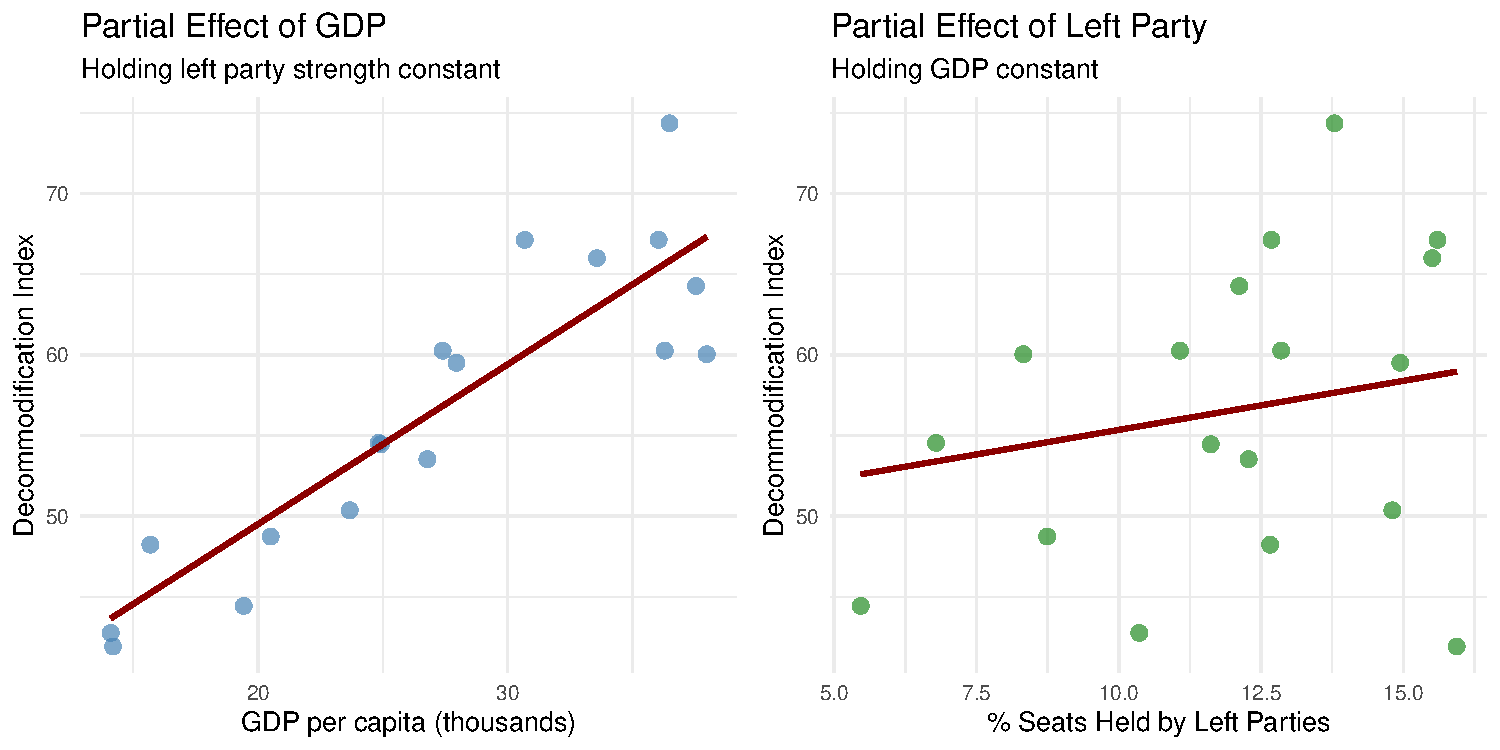
\includegraphics[keepaspectratio]{index_files/figure-pdf/fig-partial-effects-1.pdf}}

}

\caption{\label{fig-partial-effects}Partial effects of GDP and left
party strength on welfare state generosity.}

\end{figure}%

These plots show the \textbf{partial relationship} between each
predictor and the outcome. The slope of each line represents the
corresponding regression coefficient.

\begin{center}\rule{0.5\linewidth}{0.5pt}\end{center}

\section{Understanding Matrix
Operations}\label{understanding-matrix-operations}

For those interested in the computational details, here is a brief
primer on the matrix operations used in multivariate regression.

\subsection{Addition and Subtraction}\label{addition-and-subtraction}

Matrices of the same dimensions can be added or subtracted element-wise:

\[
\begin{pmatrix} 3 & -2 & 7 \\ 4 & 1 & -5 \end{pmatrix} + \begin{pmatrix} 2 & 6 & -1 \\ -3 & 4 & 8 \end{pmatrix} = \begin{pmatrix} 5 & 4 & 6 \\ 1 & 5 & 3 \end{pmatrix}
\]

\subsection{Multiplication}\label{multiplication}

To multiply two matrices, the number of columns in the first matrix must
equal the number of rows in the second. The resulting matrix has
dimensions determined by the outer dimensions.

Example: Example:

\[
\begin{pmatrix} 3 & -1 \\ 2 & 4 \end{pmatrix} \begin{pmatrix} 5 & 2 & -3 \\ 1 & -2 & 4 \end{pmatrix} = \begin{pmatrix} 3(5) + (-1)(1) & 3(2) + (-1)(-2) & 3(-3) + (-1)(4) \\ 2(5) + 4(1) & 2(2) + 4(-2) & 2(-3) + 4(4) \end{pmatrix}
\]

\[
= \begin{pmatrix} 14 & 8 & -13 \\ 14 & -4 & 10 \end{pmatrix}
\]

\[
= \begin{pmatrix} 11 & 0 & 21 \\ -1 & 13 & -9 \end{pmatrix}
\]

\subsection{Transposition}\label{transposition}

The \textbf{transpose} of a matrix \(\mathbf{A}\), denoted
\(\mathbf{A}'\), is obtained by flipping rows and columns:

\[
\mathbf{A} = \begin{pmatrix} 6 & -3 \\ 2 & 5 \\ -1 & 4 \end{pmatrix} \quad \Rightarrow \quad \mathbf{A}' = \begin{pmatrix} 6 & 2 & -1 \\ -3 & 5 & 4 \end{pmatrix}
\]

\subsection{Matrix Inverse}\label{matrix-inverse}

The \textbf{inverse} of a matrix \(\mathbf{A}\), denoted
\(\mathbf{A}^{-1}\), satisfies:

\[
\mathbf{A} \mathbf{A}^{-1} = \mathbf{A}^{-1} \mathbf{A} = \mathbf{I}
\]

where \(\mathbf{I}\) is the \textbf{identity matrix} (a square matrix
with 1's on the diagonal and 0's elsewhere).

For a \(2 \times 2\) matrix:

\[
\mathbf{A} = \begin{pmatrix} a & b \\ c & d \end{pmatrix}
\]

the inverse (if it exists) is:

\[
\mathbf{A}^{-1} = \frac{1}{ad - bc} \begin{pmatrix} d & -b \\ -c & a \end{pmatrix}
\]

Example:

\[
\mathbf{A} = \begin{pmatrix} 3 & 4 \\ 2 & 3 \end{pmatrix} \quad \Rightarrow \quad \mathbf{A}^{-1} = \frac{1}{3(3) - 4(2)} \begin{pmatrix} 3 & -4 \\ -2 & 3 \end{pmatrix} = \frac{1}{1} \begin{pmatrix} 3 & -4 \\ -2 & 3 \end{pmatrix} = \begin{pmatrix} 3 & -4 \\ -2 & 3 \end{pmatrix}
\]

(since \(3(3) - 4(2) = 9 - 8 = 1\)).

(since \(2(-7) - 5(-3) = -14 + 15 = 1\)).

\begin{center}\rule{0.5\linewidth}{0.5pt}\end{center}

\section{Summary}\label{summary-3}

Multivariate regression extends the logic of bivariate regression to
multiple predictors, allowing us to estimate the \emph{independent}
association of each variable with the outcome while controlling for
others. This chapter introduced:

\begin{itemize}
\tightlist
\item
  The \textbf{multivariate regression equation}:
  \(y = \beta_0 + \beta_1 x_1 + \beta_2 x_2 + \ldots + \beta_k x_k + e\)
\item
  \textbf{Interpretation of coefficients}: each \(\beta_j\) represents
  the expected change in \(y\) for a one-unit increase in \(x_j\),
  \emph{holding all other variables constant}
\item
  \textbf{Matrix notation}:
  \(\mathbf{y} = \mathbf{X} \boldsymbol{\beta} + \mathbf{e}\), which
  provides a compact and elegant way to express multivariate models
\item
  \textbf{Estimation}:
  \(\hat{\boldsymbol{\beta}} = (\mathbf{X}'\mathbf{X})^{-1} \mathbf{X}' \mathbf{y}\),
  the matrix solution to the least squares problem
\item
  \textbf{Inference}: hypothesis tests for individual coefficients using
  \(t\)-statistics, and overall model significance using the
  \(F\)-statistic
\item
  \textbf{Goodness-of-fit}: \(R^2\) measures the proportion of variance
  explained by the model
\item
  \textbf{Model assumptions}: correct specification, independent and
  normally distributed errors, zero mean, constant variance, and
  exogeneity
\end{itemize}

Multivariate regression is the foundation of modern empirical social
science. It allows us to disentangle complex, overlapping influences and
to estimate causal effects in observational data. However, regression is
only as good as the assumptions it rests on. Careful attention to
specification, measurement, and diagnostics is essential for valid
inference.

\begin{center}\rule{0.5\linewidth}{0.5pt}\end{center}

\section{Further Reading}\label{further-reading}

\begin{itemize}
\tightlist
\item
  Fox, J. (2016). \emph{Applied Regression Analysis and Generalized
  Linear Models} (3rd ed.). Sage.
\item
  Gelman, A., \& Hill, J. (2007). \emph{Data Analysis Using Regression
  and Multilevel/Hierarchical Models}. Cambridge University Press.
\item
  Wooldridge, J. M. (2020). \emph{Introductory Econometrics: A Modern
  Approach} (7th ed.). Cengage Learning.
\end{itemize}

\begin{center}\rule{0.5\linewidth}{0.5pt}\end{center}




\end{document}
